% ThinkAlgo — Thinking Mathematics Grade 7 — Teacher book -- with detailed solutions
%% Generated by build_grade7.py — edit grade7/body/ and rebuild.
\documentclass[11pt]{article}
\newif\ifsol \soltrue
\usepackage{iftex}
\ifPDFTeX
  \usepackage[utf8]{inputenc}\usepackage[T5]{fontenc}
\else
  \usepackage{fontspec}
\fi
\usepackage[a4paper,top=2.95cm,headheight=1.5cm,headsep=0.45cm,bottom=3.1cm,left=1.9cm,right=1.9cm]{geometry}
\usepackage{amsmath,amssymb}
\usepackage{tikz}\usetikzlibrary{calc,shadows,shapes.geometric}
\usepackage[most]{tcolorbox}
\usepackage{enumitem}
\usepackage{array}
\usepackage{tabularx}
\usepackage{colortbl}
\usepackage{comment}
\usepackage{needspace}
\usepackage{fancyhdr}
\usepackage{fontawesome5}
\usepackage{graphicx}
\usepackage{microtype}
% PDF outline (bookmarks) so each chapter shows in the reader's outline — does not change the page layout
\usepackage[hidelinks,unicode,bookmarksnumbered=false,bookmarksopen=true,bookmarksopenlevel=0]{hyperref}
\usepackage{bookmark}
\usetikzlibrary{decorations.pathreplacing,arrows.meta,angles,quotes,patterns,positioning,through,intersections}

% ---------------- palette: navy family + subtle light tint; orange ONLY in the logo ----------------
% ----- EXACT palette from the user's original main (36).tex (vivid, not pale) -----
\definecolor{tmBlue}{RGB}{66,133,244}   % problem / header / section
\definecolor{tmGreen}{RGB}{52,168,83}   % solution
\definecolor{tmOrange}{RGB}{255,152,0}  % example
\colorlet{Navy}{tmBlue}                 % header rule / section heading / badge / divider
\definecolor{NavyD}{HTML}{222222}       % solution body text (dark, readable)
\colorlet{Gold}{Navy}
\colorlet{ProbBlue}{tmBlue}             % problem boxes
\colorlet{SolGreen}{tmGreen}            % solution boxes
\definecolor{AnsRed}{HTML}{E02424}      % vivid red for answers / totals
\definecolor{CardGreen}{HTML}{34A853}   % digit-card green
\definecolor{StarGold}{HTML}{F2B134}    % difficulty star (gold)
\definecolor{KidOrange}{HTML}{DE8A2C}   % logo accent only
\definecolor{Ink}{HTML}{1F2733}       % body text
\definecolor{Slate}{HTML}{5B6A82}     % muted labels
\definecolor{Line}{HTML}{C6D0DF}      % light hairlines / student boxes
\definecolor{Tint}{HTML}{EDF1F7}      % pale panel fill (worked solution / answer)
% aliases so older names keep working
\colorlet{TextDark}{Ink}\colorlet{TextGray}{Slate}\colorlet{Soft}{Slate}
\colorlet{CardLine}{Line}\colorlet{Teal}{Navy}\colorlet{ProbB}{Navy}\colorlet{SolG}{Navy}
% bright, kid-friendly colours for bar-model (sơ đồ đoạn thẳng) blocks
\definecolor{tmPurple}{RGB}{124,77,226}
\definecolor{tmTeal}{RGB}{0,150,136}
\definecolor{tmPink}{RGB}{233,30,99}
\AtBeginDocument{\color{Ink}}
\raggedbottom  % natural flow, even spacing (no stretched gaps)
\setlength{\parindent}{0pt}\setlength{\parskip}{0.18em}
\renewcommand{\arraystretch}{1.35}
\providecommand{\AnsWord}{Đáp số}

% ---------------- brand logo (original mark) ----------------
\newcommand{\logomark}[1]{\begin{tikzpicture}[baseline=-0.55ex,scale=#1]
  \draw[KidOrange,line width=1.5pt] (-0.27,0) .. controls (-0.27,0.23) and (0,0.23) .. (0,0)
        .. controls (0,-0.23) and (-0.27,-0.23) .. (-0.27,0);
  \draw[Navy,line width=1.5pt] (0.27,0) .. controls (0.27,0.23) and (0,0.23) .. (0,0)
        .. controls (0,-0.23) and (0.27,-0.23) .. (0.27,0);
\end{tikzpicture}}
% real brand logo image (gold infinity + "think algo" wordmark)
\newcommand{\logohead}{\IfFileExists{logo.png}{\includegraphics[height=1.35cm]{logo.png}}%
  {\raisebox{0.35cm}{\logomark{1.5}\hspace{0.5em}{\Large\bfseries\color{KidOrange}think\,\color{Navy}algo}}}}

% ---------------- running header (logo + Name/Date + topic) on EVERY page, single navy rule ----------------
\pagestyle{fancy}\fancyhf{}
\renewcommand{\headrulewidth}{1.4pt}\renewcommand{\footrulewidth}{0pt}
\renewcommand{\headrule}{{\color{Navy}\hrule height 1.3pt}}
\fancyhead[L]{\raisebox{-0.95cm}{\logohead}}
\fancyhead[R]{\setlength{\tabcolsep}{0pt}%
  \begin{tabular}{@{}r@{}}
    {\small\color{Ink}{\color{tmBlue}\faUserEdit}~\NameWord:~\rule{3.0cm}{0.5pt}\quad{\color{tmBlue}\faCalendarDay}~\DateWord:~\rule{1.9cm}{0.5pt}}\\[5pt]
    {\large\bfseries\color{Navy}\CurTopic}
  \end{tabular}}

% ---------------- footer (rounded page border + Topic/Grade + thinkalgo.com + page + tagline) ----------------
% NOTE: a remember-picture overlay must be placed DIRECTLY in \fancyfoot, NOT inside \def/\newcommand.
\fancyfoot[C]{\begin{tikzpicture}[remember picture, overlay]
  \draw[Navy!40, line width=1.4pt, rounded corners=12pt]
     ($(current page.north west)+(0.8cm,-0.8cm)$) rectangle ($(current page.south east)+(-0.8cm,0.45cm)$);
  \coordinate (FL) at ($(current page.south west)+(1.2cm, 2.18cm)$);
  \coordinate (FR) at ($(current page.south east)+(-1.2cm, 2.18cm)$);
  \draw[Navy!55, line width=1pt] (FL) -- (FR);
  \node[fill=white, draw=Navy, line width=1.2pt, rounded corners=8pt, font=\bfseries\small,
        text=Navy, inner xsep=11pt, inner ysep=4pt] at ($(current page.south)+(0,2.18cm)$) {{\color{tmBlue}\faGlobe}\ \ thinkalgo.com};
  \node[text=Slate, font=\footnotesize, anchor=north west, align=left, inner sep=0pt, text width=7.6cm]
        at ($(FL)+(0.1cm,-0.30cm)$) {{\color{tmBlue}\faTag}\ \TopicWord: \textbf{\color{Ink}\CurTopic}\\[1.5pt]{\color{tmBlue}\faGraduationCap}\ \DocGrade};
  \node[text=Slate, font=\footnotesize] at ($(current page.south)+(0,1.20cm)$) {\thepage};
  \node[text=Slate, font=\scriptsize, anchor=north east, align=right, inner sep=0pt, text width=7.4cm]
        at ($(FR)+(-0.1cm,-0.34cm)$) {{\normalsize\bfseries\color{Navy}ThinkAlgo}\ — From Math Thinking to Code};
\end{tikzpicture}}

% ---------------- page-1 lead-in (topic is already in the header; keep a slim spacer) ----------------
\newcommand{\titlehead}{\vspace*{-0.2cm}}
\providecommand{\CurTopic}{}

% chapter banner + sets the running-header topic. #1 = number, #2 = title
\newcommand{\chapterhead}[2]{\renewcommand{\CurTopic}{#2}%
  \setcounter{seccnt}{0}% each chapter is independent: section badges restart at 1
  \phantomsection\pdfbookmark[0]{#1. #2}{chap#1}\label{chap:#1}% add this chapter to the PDF outline + TOC ref
  \par\vspace{0.1cm}\noindent\begin{tikzpicture}[baseline=-0.5ex]
    \node[circle,fill=tmBlue,text=white,font=\Large\bfseries,minimum size=0.95cm,inner sep=0pt](cn){#1};
    \node[anchor=west,font=\LARGE\bfseries,text=tmBlue] at ([xshift=12pt]cn.east){#2};
  \end{tikzpicture}\par\vspace{4pt}\noindent\textcolor{tmBlue}{\rule{\linewidth}{2pt}}\par\vspace{0.5cm}}

% ---------------- section heading (outline navy number badge, no fill) ----------------
\newcounter{seccnt}
\newcommand{\shead}[1]{\par\vspace{0.7em}\refstepcounter{seccnt}%
  \noindent
\begin{tikzpicture}[baseline=-0.6ex]
    \node[circle,draw=Gold,line width=1.2pt,text=Gold,font=\bfseries,minimum size=1.05em,inner sep=1pt]{\theseccnt};
  \end{tikzpicture}\hspace{0.4em}{\large\bfseries\color{Navy} #1}\par\vspace{0.25em}}

% ============ boxes EXACTLY per the original main (36).tex: solid-blue PROBLEM, solid-orange EXAMPLE,
%              outline-green SOLUTION, all with drop shadow + rounded corners ============
% ---------------- knowledge box: white, tmBlue border + left accent + drop shadow ----------------
\newtcolorbox{knowbox}{enhanced,breakable,colback=white,colframe=tmBlue!70,boxrule=0.9pt,arc=5pt,
  left=12pt,right=11pt,top=6pt,bottom=6pt,drop shadow,
  borderline west={3.5pt}{0pt}{tmBlue}}

% ---------------- EXAMPLE (Ví dụ): SOLID ORANGE tab, white text ----------------
\newtcolorbox{exbox}[1]{enhanced,breakable,colback=white,colframe=tmOrange,boxrule=1pt,arc=5pt,
  left=12pt,right=11pt,top=14pt,bottom=7pt,drop shadow,
  attach boxed title to top left={xshift=10pt,yshift=-\tcboxedtitleheight/2},
  boxed title style={colback=tmOrange,colframe=tmOrange,arc=4pt,boxrule=0pt,drop shadow},
  title={#1},fonttitle=\bfseries\color{white}}
\newcommand{\guide}{\par\vspace{2pt}{\bfseries\color{tmBlue}\GuideWord}\par\nopagebreak}

% ---------------- PROBLEM (Bài): SOLID BLUE tab, white text ----------------
\newtcolorbox{probbox}[2]{enhanced,breakable,colback=white,colframe=tmBlue,boxrule=1pt,arc=5pt,
  left=12pt,right=10pt,top=14pt,bottom=7pt,drop shadow,
  attach boxed title to top left={xshift=10pt,yshift=-\tcboxedtitleheight/2},
  boxed title style={colback=tmBlue,colframe=tmBlue,arc=4pt,boxrule=0pt,drop shadow},
  fonttitle=\bfseries\color{white},title={\ProbWord\ #1\ifx\relax#2\relax\else#2\fi}}

% ---------------- SOLUTION (Lời giải): OUTLINE GREEN tab (white fill, green border + text) ----------------
% Teacher: a green tcolorbox. Student: the body is dropped entirely (comment pkg — robust with tables/\\).
\ifsol
  \newtcolorbox{solbox}{enhanced,breakable,colback=white,colframe=tmGreen,boxrule=1pt,arc=5pt,
    left=12pt,right=10pt,top=14pt,bottom=7pt,drop shadow,
    attach boxed title to top left={xshift=10pt,yshift=-\tcboxedtitleheight/2},
    boxed title style={colback=white,colframe=tmGreen,boxrule=1pt,arc=4pt,drop shadow},
    fonttitle=\bfseries\color{tmGreen!88!black},title={\SolTitle},before upper={\color{NavyD}}}
\else
  \excludecomment{solbox}
\fi

% ---------------- answer highlight: label green, value RED ----------------
\newcommand{\ans}[1]{\par\smallskip{\bfseries\color{tmGreen!88!black}\AnsWord:}\ {\bfseries\color{AnsRed}#1}\par}

% ---------------- digit cards (exact original style: fill=c!10, border=c!60!black, drop shadow) ----------------
% \digitcards{0/gray,1/cyan,2/green,3/cyan} : value/colour pairs
\newcommand{\digitcards}[1]{\begin{center}\begin{tikzpicture}[scale=0.7,transform shape,font=\sffamily]
  \def\dx{0}\foreach \v/\c in {#1}{
    \node[draw=\c!60!black,line width=1.5pt,fill=\c!10,rounded corners=4pt,
          minimum width=1cm,minimum height=1.4cm,drop shadow] at (\dx,0){\Huge\bfseries \v};
    \pgfmathsetmacro\dx{\dx+1.5}\xdef\dx{\dx}}
\end{tikzpicture}\end{center}}

% ---------------- student working space (white, light border) ----------------
\newcommand{\worksp}[1]{\ifsol\else\begin{tcolorbox}[colback=white,colframe=Line,boxrule=0.8pt,
  arc=5pt,height=\dimexpr#1+0.05cm\relax,left=8pt,right=8pt,top=4pt,bottom=4pt]{\footnotesize\color{Slate}\itshape\WorkWord}\end{tcolorbox}\fi}

% ---------------- \probsol{solution} : Teacher shows the green solution box; Student shows a BLANK
%   "Bài làm" box whose height matches that solution's height (writing room = work needed), so both
%   versions have identical per-problem height and paginate the same. ----------------
\newsavebox{\solmeasure}\newlength{\solht}
\newcommand{\probsol}[1]{%
  \begin{lrbox}{\solmeasure}\begin{minipage}{\dimexpr\linewidth-24pt\relax}#1\end{minipage}\end{lrbox}%
  \ifsol
    \begin{solbox}#1\end{solbox}%
  \else
    \setlength{\solht}{\dimexpr\ht\solmeasure+\dp\solmeasure+0.85cm\relax}%
    \ifdim\solht<1.35cm\setlength{\solht}{1.35cm}\fi
    \ifdim\solht>\StudentMaxWork\setlength{\solht}{\StudentMaxWork}\fi
    \begin{tcolorbox}[colback=white,colframe=Line,boxrule=0.8pt,arc=5pt,
      left=8pt,right=8pt,top=4pt,bottom=4pt,height=\solht]{\footnotesize\color{Slate}\itshape\WorkWord}\end{tcolorbox}%
  \fi}

% ---------------- practice divider: blue left accent bar, no fill ----------------
\newcommand{\dividerbar}[1]{\par\vspace{0.6em}\noindent
  \begin{tcolorbox}[enhanced,frame hidden,interior hidden,borderline west={5pt}{0pt}{ProbBlue},
    colback=white,left=12pt,right=12pt,top=5pt,bottom=5pt,arc=4pt]
  {\large\bfseries\color{ProbBlue} #1}\end{tcolorbox}\vspace{0.4em}}

% place-value choice-count diagram (Cambridge style): #1 = "label/count/note/color" list, #2 = result
% notes must NOT contain commas or slashes (they separate \foreach fields)
\newcommand{\countboxes}[2]{\begin{center}\begin{tikzpicture}[scale=0.62,transform shape,font=\sffamily]
  \def\xx{0}%
  \foreach \lab/\cnt/\note/\col [count=\i] in {#1}{%
    \ifnum\i>1\relax \node[text=gray,font=\Huge] at (\xx-1.8,0){$\times$};\fi
    \node[draw=\col!65,fill=\col!8,rounded corners=3pt,line width=1pt,minimum width=2.7cm,minimum height=1.7cm] at (\xx,0){};
    \node[text=\col!85,font=\bfseries] at (\xx,0.58){\lab};
    \node[text=\col!88,font=\Huge\bfseries] at (\xx,-0.1){\cnt};
    \node[text=gray,font=\scriptsize] at (\xx,-1.05){\note};
    \pgfmathsetmacro\xx{\xx+3.6}\xdef\xx{\xx}}%
  \node[text=gray,font=\Huge] at (\xx-1.8,0){$=$};
  \node[text=red,font=\Huge\bfseries] at (\xx,0){#2};
\end{tikzpicture}\end{center}}

% ======== bar model (sơ đồ đoạn thẳng): lightly-rounded blocks, darker border, tiny gaps, bright colours ========
% one block: \blk{x1}{x2}{yc}{height}{colour}{label}  (a small gap is left on each side)
\newcommand{\blk}[6]{%
  \draw[rounded corners=1.3pt,fill=#5!16,draw=#5!80!black,line width=1pt]
    (#1+0.045,#3-#4/2) rectangle (#2-0.045,#3+#4/2);
  \node[font=\small\bfseries,text=#5!52!black] at ({(#1+#2)/2},#3){#6};}
% measurement with a double-headed ARROW (not a brace) + label above the span: \brcup{x1}{x2}{y}{label}
\newcommand{\brcup}[4]{%
  \draw[<->,>=stealth,tmBlue!72!black,line width=0.7pt] (#1+0.05,#3)--(#2-0.05,#3);
  \node[above=-1.5pt,font=\footnotesize,text=tmBlue!58!black] at ({(#1+#2)/2},#3){#4};}
% measurement with a double-headed ARROW + label below the span: \brcdn{x1}{x2}{y}{label}
\newcommand{\brcdn}[4]{%
  \draw[<->,>=stealth,tmBlue!72!black,line width=0.7pt] (#1+0.05,#3)--(#2-0.05,#3);
  \node[below=-1.5pt,font=\footnotesize,text=tmBlue!58!black] at ({(#1+#2)/2},#3){#4};}
% row label at the left of a bar: \rowlab{x}{y}{text}
\newcommand{\rowlab}[3]{\node[anchor=east,font=\small\bfseries,text=Ink] at (#1,#2){#3};}
% vertical right-pointing CURLY BRACE spanning two stacked bars: \vbrace{x}{ytop}{ybot}{label}
\newcommand{\vbrace}[4]{%
  \pgfmathsetmacro\ym{(#2+#3)/2}%
  \draw[tmBlue!72!black,line width=0.9pt,line cap=round]
    (#1,#2) .. controls (#1+0.18,#2) and (#1+0.18,#2-0.18) .. (#1+0.18,#2-0.22)
    -- (#1+0.18,{\ym+0.22})
    .. controls (#1+0.18,\ym) and (#1+0.30,{\ym+0.08}) .. (#1+0.42,\ym)
    .. controls (#1+0.30,{\ym-0.08}) and (#1+0.18,\ym) .. (#1+0.18,{\ym-0.22})
    -- (#1+0.18,#3+0.22)
    .. controls (#1+0.18,#3+0.18) and (#1+0.18,#3) .. (#1,#3);
  \node[right=4pt,font=\footnotesize,text=tmBlue!58!black] at (#1+0.42,\ym){#4};}
% blank 3x3 grid for a problem statement (student fills it in)
\newcommand{\blankgrid}{
\begin{tikzpicture}[font=\sffamily]
  \foreach \r in {0,1,2}{\foreach \c in {0,1,2}{
    \draw[rounded corners=1.3pt,fill=Tint,draw=Slate!55,line width=0.9pt]
      (\c+0.05,\r+0.05) rectangle (\c+0.95,\r+0.95);}}
\end{tikzpicture}}
% wrapper: LEFT-aligned (not centred), a little air above/below
\newenvironment{barfig}{\par\vspace{3pt}\noindent\kern0.35cm\begin{tikzpicture}[font=\sffamily,>=stealth]}%
  {\end{tikzpicture}\par\vspace{3pt}}
% wrapper: CENTRED (for illustrative diagrams in theory / examples)
\newenvironment{barfigC}{\par\vspace{3pt}\begin{center}\begin{tikzpicture}[font=\sffamily,>=stealth]}%
  {\end{tikzpicture}\end{center}\vspace{2pt}}

% ---------------- difficulty stars (nicely drawn) : \stars{1}=hard, \stars{2}=very hard ----------------
\newcommand{\diffstar}{\tikz[baseline=-0.55ex]{\node[star,star points=5,star point ratio=0.46,
  draw=StarGold!72!black,fill=StarGold,line width=0.3pt,inner sep=1.75pt]{};}}
\newcommand{\stars}[1]{\ifcase#1\or\kern2pt\diffstar\or\kern2pt\diffstar\kern1.5pt\diffstar\fi}

\newcommand{\nd}[1]{\overline{#1}}

% number line: #1 last index, #2 ticks "i/label", #3 open (excluded) indices, #4 filled (solution) indices
\newcommand{\numlinex}[4]{\begin{center}\begin{tikzpicture}[x=1.55cm,>=stealth]
  \draw[->,thick,Navy](-0.45,0)--(#1+0.45,0);
  \foreach \i/\lab in {#2}{\draw[Navy,line width=0.8pt](\i,0.08)--(\i,-0.08);
     \node[below,font=\small,text=Ink]at(\i,-0.1){\lab};}
  \foreach \i in {#3}{\draw[Navy,fill=white,line width=1pt](\i,0)circle(2.3pt);}
  \foreach \i in {#4}{\fill[KidOrange](\i,0)circle(2.7pt);}
\end{tikzpicture}\end{center}}


% ======================================================================
% Grade 7 additions (shared by all four editions)
% ======================================================================
% student edition: blank "work" box height = min(solution height, this cap)
\newlength{\StudentMaxWork}\setlength{\StudentMaxWork}{7.5cm}

% ThinkAlgo tip box (label set per language by \TipWord)
\newtcolorbox{tipbox}{enhanced,breakable,colback=StarGold!8,colframe=StarGold!75!black,boxrule=1pt,arc=4pt,
  left=11pt,right=10pt,top=6pt,bottom=6pt,
  before upper={\textbf{\color{StarGold!65!black}\faLightbulb\ \TipWord}\ }}

% "Recall" box: re-states a piece of theory inside a solution / example
\newtcolorbox{recallbox}{enhanced,breakable,colback=tmBlue!5,colframe=tmBlue!45,boxrule=0.6pt,arc=3pt,
  left=8pt,right=8pt,top=4pt,bottom=4pt,
  before upper={\textbf{\color{tmBlue!80!black}\faBookOpen\ \RecallWord}\ }}

% "Why is it true? / Proof" box
\newtcolorbox{proofbox}{enhanced,breakable,colback=tmPurple!4,colframe=tmPurple!45,boxrule=0.6pt,arc=3pt,
  left=8pt,right=8pt,top=4pt,bottom=4pt,
  before upper={\textbf{\color{tmPurple!85!black}\faSearch\ \ProofWord}\ },
  after upper={\hfill$\square$}}

% "Common mistake" box
\newtcolorbox{warnbox}{enhanced,breakable,colback=AnsRed!4,colframe=AnsRed!45,boxrule=0.6pt,arc=3pt,
  left=8pt,right=8pt,top=4pt,bottom=4pt,
  before upper={\textbf{\color{AnsRed!85!black}\faExclamationTriangle\ \WarnWord}\ }}

% "Note for parents" box (short hint on how to explain the idea at home)
\newtcolorbox{parentbox}{enhanced,breakable,colback=tmTeal!5,colframe=tmTeal!50,boxrule=0.6pt,arc=3pt,
  left=8pt,right=8pt,top=4pt,bottom=4pt,
  before upper={\textbf{\color{tmTeal!80!black}\faUsers\ \ParentWord}\ }}

% numbered step inside a solution:  \step{1}{Short title}  -> "Bước 1. Short title"
\newcommand{\step}[2]{\par\smallskip\noindent{\bfseries\color{tmBlue!85!black}\StepWord~#1.}\ {\bfseries #2}\par\nopagebreak}
% verification line:  \verify{...}
\newcommand{\verify}[1]{\par\smallskip\noindent{\bfseries\color{tmGreen!80!black}\faCheckCircle\ \CheckWord}\ #1\par}

% multiple-choice options
% \choices{..}{..}{..}{..}{..}      : five short options on one line
% \choicesII{..}{..}{..}{..}{..}    : two/three per line (medium length)
% \choicesL{..}{..}{..}{..}{..}     : one option per line (long text)
\newcommand{\choices}[5]{\par\smallskip\noindent
  \begin{tabularx}{\linewidth}{@{}XXXXX@{}}(A)\ #1&(B)\ #2&(C)\ #3&(D)\ #4&(E)\ #5\end{tabularx}\par}
\newcommand{\choicesII}[5]{\par\smallskip\noindent
  \begin{tabularx}{\linewidth}{@{}XXX@{}}(A)\ #1&(B)\ #2&(C)\ #3\\(D)\ #4&(E)\ #5&\end{tabularx}\par}
\newcommand{\choicesL}[5]{\par\smallskip\noindent
  \begin{tabular}{@{}l@{}}(A)\ #1\\(B)\ #2\\(C)\ #3\\(D)\ #4\\(E)\ #5\end{tabular}\par}

% centred figure inside a problem / solution
\newenvironment{figC}{\par\vspace{2pt}\begin{center}\begin{tikzpicture}[font=\sffamily\small,>=stealth,line join=round]}%
  {\end{tikzpicture}\end{center}\vspace{1pt}}


% table-of-contents line: \tocline{n}{title} -> badge, title, dotted leader, page (via \label{chap:n})
\newcommand{\tocline}[2]{\par\noindent
  \begin{tikzpicture}[baseline=-0.6ex]\node[circle,fill=tmBlue,text=white,font=\bfseries,
    minimum size=0.75cm,inner sep=0pt]{#1};\end{tikzpicture}\hspace{0.6em}%
  {\large\bfseries\color{Ink}\hyperref[chap:#1]{#2}}\ \dotfill\ {\large\bfseries\color{tmBlue}\pageref{chap:#1}}\par\vspace{0.3cm}}

\def\DocGrade{Grade 7}
\def\ProbWord{Problem}
\def\SolWord{Solution.}
\def\GuideWord{Guided solution.}
\def\PageWord{Page}
\def\NameWord{Name}
\def\DateWord{Date}
\def\SolTitle{Detailed solution}
\def\WorkWord{Your work:}
\def\TopicWord{Topic}
\def\AnsWord{Answer}
\def\TipWord{ThinkAlgo Tip.}
\def\RecallWord{Recall.}
\def\ProofWord{Why is it true?}
\def\WarnWord{Common mistake.}
\def\ParentWord{Note for parents.}
\def\StepWord{Step}
\def\CheckWord{Check:}

\def\DocTopic{Thinking Mathematics Grade 7}
\begin{document}

% ---------------- cover + contents ----------------
\renewcommand{\CurTopic}{Thinking Mathematics Grade 7}
\thispagestyle{empty}
\begin{tikzpicture}[remember picture,overlay]
  \fill[tmBlue] (current page.north west) rectangle ([yshift=-9.5cm]current page.north east);
  \fill[tmBlue!80!black] ([yshift=-9.5cm]current page.north west) rectangle ([yshift=-9.9cm]current page.north east);
  \fill[KidOrange] ([yshift=-9.9cm]current page.north west) rectangle ([yshift=-10.1cm]current page.north east);
  \node[anchor=north west,text=white,font=\Large\bfseries] at ([xshift=2cm,yshift=-1.6cm]current page.north west)
     {think\,algo};
  \node[anchor=north west,text=white,font=\fontsize{34}{40}\selectfont\bfseries,text width=16cm]
     at ([xshift=2cm,yshift=-3.6cm]current page.north west) {Thinking Mathematics Grade 7};
  \node[anchor=north west,text=white,font=\large,text width=16cm]
     at ([xshift=2cm,yshift=-6.2cm]current page.north west) {Theory -- Worked examples -- 250 practice and challenge problems};
  \node[anchor=north west,fill=white,text=tmBlue,font=\bfseries,rounded corners=6pt,inner xsep=10pt,inner ysep=6pt]
     at ([xshift=2cm,yshift=-7.6cm]current page.north west) {Teacher book -- with detailed solutions};
  \node[anchor=south,text=Slate,font=\small] at ([yshift=1.6cm]current page.south)
     {ThinkAlgo --- From Math Thinking to Code \quad\textbullet\quad thinkalgo.com};
\end{tikzpicture}\par
\vspace*{7.0cm}
{\Large\bfseries\color{Navy}Contents}\par\vspace{2pt}
{\color{tmBlue}\rule{\linewidth}{1.5pt}}\par\vspace{0.4cm}
\tocline{1}{Algebra and Equations}
\tocline{2}{Geometry and Measurement}
\tocline{3}{Counting and Probability}
\tocline{4}{Number Sense}
\tocline{5}{Logic and Puzzles}
\vspace{0.4cm}
\begin{tipbox}
\begin{itemize}[leftmargin=1.2em,itemsep=2pt,topsep=2pt]
\item Each chapter contains: \textbf{theory} (with explanations and proofs), \textbf{worked examples} with guided solutions, and \textbf{50 problems}: \emph{Core practice} followed by \emph{Extension and challenge}.
\item Problems marked \stars{1} are hard, \stars{2} very hard.
\item Try each problem on your own first, then compare with the solution.
\end{itemize}
\end{tipbox}

% ================= CHAPTER 1: Algebra and Equations =================
\clearpage
\renewcommand{\arraystretch}{1.35}
\chapterhead{1}{Algebra and Equations}

% ---------------- part a ----------------
% ===================== Topic 1 -- Algebra and Equations -- part a (EN) =====================
% helper macros (topic prefix \aea..., guarded)
% \aeaBox{a}{b}{c}{d}: a 2x2 box holding four numbers (Problems 14, 33)
\providecommand{\aeaBox}[4]{\begin{tikzpicture}[baseline=-0.7ex,font=\small]
  \draw[Navy,line width=0.8pt,fill=tmBlue!6] (-0.66,-0.32) rectangle (0.66,0.32);
  \draw[Navy,line width=0.8pt] (0,-0.32)--(0,0.32) (-0.66,0)--(0.66,0);
  \node[inner sep=0pt] at (-0.33,0.16){$#1$};\node[inner sep=0pt] at (0.33,0.16){$#2$};
  \node[inner sep=0pt] at (-0.33,-0.16){$#3$};\node[inner sep=0pt] at (0.33,-0.16){$#4$};\end{tikzpicture}}
% \aeaScale{left}{right}: a balanced scale with objects on both pans
\providecommand{\aeaScale}[2]{\begin{tikzpicture}[baseline=0pt,font=\small]
  \draw[Ink,line width=1.1pt] (-1.7,0)--(1.7,0);
  \fill[Slate] (0,0)--(-0.22,-0.38)--(0.22,-0.38)--cycle;
  \draw[Slate,line width=1pt] (-0.4,-0.38)--(0.4,-0.38);
  \node[above=1pt] at (-1.05,0){#1};\node[above=1pt] at (1.05,0){#2};\end{tikzpicture}}
% coloured shapes for the balance problems
\providecommand{\aeaTri}{\textcolor{tmOrange}{\scalebox{1.5}{$\blacktriangle$}}}
\providecommand{\aeaSq}{\textcolor{tmBlue}{\scalebox{1.5}{$\blacksquare$}}}
\providecommand{\aeaCir}{\textcolor{tmGreen}{\scalebox{2.6}{$\bullet$}}}

\begin{knowbox}
\textbf{The big idea.} Algebra is \emph{the language of unknown numbers}. Instead of saying at length
``some number, add $5$, then double it'', we simply write $2(x+5)$. The letter $x$ (called a
\textbf{variable} or an \textbf{unknown}) holds the place of a number that we do not know yet or that may change.

In this topic you will practise four core skills:
\begin{enumerate}[leftmargin=1.4em,itemsep=1pt,topsep=2pt]
\item \textbf{Translate} words into expressions and formulas (``more than'', ``times'', ``sum'', ``difference''...).
\item \textbf{Substitute} numbers to evaluate an expression, or to check whether an equation is true or false.
\item \textbf{Solve equations} with the \emph{balance principle}: whatever you do to one side, do exactly the same to the other side.
\item \textbf{Spot patterns}: sequences, tables of values, ratios, and the order of numbers.
\end{enumerate}
Every word problem follows the same route: \emph{read carefully $\to$ choose an unknown $\to$ write an expression
or an equation $\to$ solve $\to$ check $\to$ answer}.
\end{knowbox}
\vspace{0.3cm}

% ------------------------------------------------------------------------------------------
\needspace{6\baselineskip}\shead{Variables, algebraic expressions and formulas}
\begin{knowbox}
\textbf{1. Variables and expressions.} An \textbf{algebraic expression} is built from numbers, letters
(variables) and the operations $+,\ -,\ \times,\ \div$, powers and brackets. Examples: $3x-1$;\quad $2(n-1)$;\quad $120+30m$;\quad $xy$.

\textbf{Short-hand.} Between a number and a letter, or between two letters, we leave out the multiplication sign:
$3x$ means $3\cdot x$;\ \ $xy$ means $x\cdot y$;\ \ $2(n-1)$ means $2\cdot(n-1)$. The number is written before the letter.

\textbf{2. Value of an expression.} To evaluate an expression for given values of the variables, we
\emph{replace} each letter by its number (best put in brackets), then calculate in the correct order of operations.

\emph{Example:} for $x=3$, $3x-1=3\cdot 3-1=9-1=8$;\quad $2x^2=2\cdot 3^2=2\cdot 9=18$.

\textbf{3. Translating words into expressions.}

\begin{center}
\begin{tabular}{|l|c|}
\hline
\rowcolor{tmBlue!10}\textbf{Words} & \textbf{Expression}\\ \hline
$5$ more than $x$;\ \ $x$ increased by $5$ & $x+5$\\ \hline
$5$ less than $x$;\ \ $x$ decreased by $5$ & $x-5$\\ \hline
$3$ times $x$;\ \ triple $x$ & $3x$\\ \hline
half of $x$;\ \ $x$ divided by $2$ & $\dfrac{x}{2}$ or $x\div 2$\\ \hline
start with $120$, add $30$ each time, $m$ times & $120+30m$\\ \hline
three consecutive whole numbers, the smallest is $n$ & $n,\ n+1,\ n+2$\\ \hline
\end{tabular}
\end{center}

\textbf{4. A formula} is an equation that tells us how to calculate one quantity from other quantities.
Useful geometry formulas (side lengths $a$, $b$, $c$):
\begin{itemize}[leftmargin=1.4em,itemsep=1pt,topsep=2pt]
\item Perimeter of a triangle: $P=a+b+c$ (the sum of the three sides).
\item Rectangle with length $a$ and width $b$: perimeter $P=2(a+b)$, area $A=a\cdot b$.
\item Triangle with base $a$ and height $h$: area $A=\dfrac{a\cdot h}{2}$.
\item Rectangular prism $a\times b\times c$: total surface area $S=2(ab+bc+ca)$, volume $V=abc$.
\end{itemize}
\end{knowbox}

\begin{proofbox}
\textbf{Why is the area of a triangle half of (base $\times$ height)?} Draw a rectangle with one side equal to the base $a$
of the triangle and the other side equal to the height $h$. The height splits the triangle into two right triangles; each right
triangle is exactly half of a smaller rectangle (in the picture, the shaded and white parts match in pairs).
So the triangle covers exactly half of the big rectangle: $A=\dfrac{a\cdot h}{2}$.
\begin{figC}
\draw[Navy,line width=0.9pt] (0,0) rectangle (4,2);
\fill[tmOrange!25] (0,0)--(4,0)--(1.4,2)--cycle;
\draw[tmOrange!80!black,line width=1pt] (0,0)--(4,0)--(1.4,2)--cycle;
\draw[dashed,Slate] (1.4,2)--(1.4,0);
\draw[Slate] (1.4,0.2)--(1.6,0.2)--(1.6,0);
\node[below] at (2,0){$a$};
\node[right] at (4,1){$h$};
\node[left,font=\footnotesize] at (1.4,1){$h$};
\end{figC}
Similarly, the perimeter of a rectangle is $a+b+a+b=2a+2b=2(a+b)$ because a rectangle has two equal long sides and two equal short sides.
\end{proofbox}

\begin{tipbox}
When substituting, \emph{always put the number in brackets}, especially a negative number: for $x=-2$,
$x^2=(-2)^2=4$, while $3x=3\cdot(-2)=-6$. Brackets protect you from sign mistakes.
\end{tipbox}

\begin{warnbox}
$3x$ with $x=4$ is $3\cdot 4=12$, \emph{not} ``$34$''. And $x^2$ (which is $x\cdot x$) is different from $2x$ (which is $x+x$):
for $x=5$, $x^2=25$ but $2x=10$.
\end{warnbox}

\begin{tipbox}
\textbf{Write everything in terms of a few letters.} Consider a list in which every number (from the third on) is the sum of the two before it.
If the first two numbers are $a$ and $b$, the next ones are
\[a,\quad b,\quad a+b,\quad b+(a+b)=a+2b,\quad (a+b)+(a+2b)=2a+3b,\ \dots\]
For instance, with $a=11$, $b=20$ the fifth number is $2\cdot 11+3\cdot 20=22+60=82$, just as in the list $11,20,31,51,82$.
Writing the numbers in terms of $a$ and $b$ turns a question about the list into an equation.
\end{tipbox}

\begin{parentbox}
Play the ``number machine'' game with your child: you say a rule (``multiply by $3$, then subtract $1$''),
your child writes it as the expression $3x-1$, and then you take turns feeding numbers into the machine. This game makes
the letter $x$ feel friendly instead of scary.
\end{parentbox}

% ------------------------------------------------------------------------------------------
\needspace{6\baselineskip}\shead{Integers, order of operations and the distributive law}
\begin{knowbox}
\textbf{1. Integers.} The numbers $\dots,-3,-2,-1,0,1,2,3,\dots$ are called integers. On the number line, a number further to the
left is smaller. The opposite of $a$ is $-a$; we have $a+(-a)=0$.
\begin{center}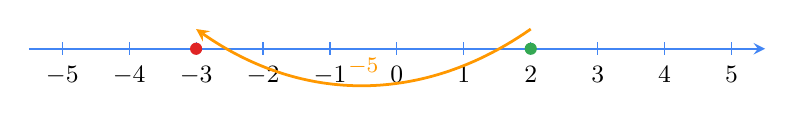
\begin{tikzpicture}[x=0.85cm,>=stealth]
\draw[->,thick,Navy] (-5.5,0)--(5.5,0);
\foreach \i in {-5,...,5}{\draw[Navy] (\i,0.08)--(\i,-0.08); \node[below,font=\small] at (\i,-0.1){$\i$};}
\draw[->,tmOrange,line width=1pt] (2,0.25) to[bend left=35] node[above,font=\footnotesize]{$-5$} (-3,0.25);
\fill[tmGreen] (2,0) circle (2.2pt); \fill[AnsRed] (-3,0) circle (2.2pt);
\end{tikzpicture}\end{center}
\emph{Example:} $2+(-5)=-3$: starting at $2$, move $5$ steps to the left and arrive at $-3$.

\textbf{2. Adding and subtracting integers.}
\begin{itemize}[leftmargin=1.4em,itemsep=1pt,topsep=2pt]
\item Two numbers with the same sign: add the sizes and keep the common sign: $(-11)+(-26)=-37$.
\item Two numbers with different signs: subtract the smaller size from the larger one and take the sign of the number with the larger size: $11+(-37)=-26$.
\item Subtracting means adding the opposite: $a-b=a+(-b)$. Example: $-26-11=-26+(-11)=-37$.
\end{itemize}

\textbf{3. Order of operations.} Brackets first $\to$ powers $\to$ multiplication and division (left to right)
$\to$ addition and subtraction (left to right). Example: $6+2\cdot 3=6+6=12$ (not $8\cdot 3$).

\textbf{4. The distributive law.} $a(b+c)=ab+ac$ and $a(b-c)=ab-ac$.
\emph{Examples:} $3(T+4)=3T+12$;\quad $20\cdot 9\,000-20\cdot 6\,750=20\cdot(9\,000-6\,750)$.

\textbf{5. Simplifying expressions.} Add ``like terms'': $3x+5x=8x$; \
$(a+1)+(b+1)+(c+1)+(d+1)=(a+b+c+d)+4$.

\textbf{6. Points in the coordinate plane.} The point $(x,y)$ has $x$-coordinate $x$ and $y$-coordinate $y$. Moving $k$ units
to the right increases $x$ by $k$; moving $k$ units up increases $y$ by $k$ (moving left or down decreases them).
\end{knowbox}

\begin{proofbox}
\textbf{Why is $a(b+c)=ab+ac$?} Take a rectangle with width $a$ and length $b+c$. Its area is
$a(b+c)$. But we can also cut it into two smaller rectangles with areas $ab$ and $ac$. It is the same
area, so $a(b+c)=ab+ac$.
\begin{figC}
\fill[tmBlue!18] (0,0) rectangle (3,1.2); \fill[tmGreen!20] (3,0) rectangle (5,1.2);
\draw[Navy,line width=0.9pt] (0,0) rectangle (5,1.2); \draw[Navy,line width=0.9pt] (3,0)--(3,1.2);
\node at (1.5,0.6){$ab$}; \node at (4,0.6){$ac$};
\node[left] at (0,0.6){$a$}; \node[below] at (1.5,0){$b$}; \node[below] at (4,0){$c$};
\end{figC}
\end{proofbox}

\begin{warnbox}
$3(T+4)$ is \emph{not} equal to $3T+4$: you must multiply $3$ by \emph{each} term inside the brackets, $3(T+4)=3T+3\cdot 4=3T+12$.
Likewise $-(a-b)=-a+b$ (change the sign of \emph{every} term in the brackets).
\end{warnbox}

% ------------------------------------------------------------------------------------------
\needspace{6\baselineskip}\shead{Equations and the balance principle}
\begin{knowbox}
\textbf{1. Equations.} A statement of equality containing an unknown, such as $2(x+8)=38$, is called an \textbf{equation}.
A number that makes both sides equal when it replaces the unknown is called a \textbf{solution}. To \emph{solve an equation} means to find its solutions.

\textbf{2. The balance principle.} Imagine the equation as a pair of scales in balance.
The scales stay balanced if we:
\begin{itemize}[leftmargin=1.4em,itemsep=1pt,topsep=2pt]
\item add (or subtract) \emph{the same number} on both sides;
\item multiply (or divide) both sides by \emph{the same non-zero number}.
\end{itemize}
A familiar consequence is the \textbf{rule for moving terms}: when a term moves from one side to the other, its \emph{sign changes}.

\begin{center}
\aeaScale{\aeaSq\,\aeaSq\ \ \fbox{\footnotesize 3 kg}}{\fbox{\footnotesize 11 kg}}
\end{center}
\emph{Example:} two identical boxes plus a $3$ kg weight balance $11$ kg: $2x+3=11$.
Remove the $3$ kg weight from both pans: $2x=11-3=8$. Halve both pans: $x=8\div 2=4$. Each box weighs $4$ kg.

\textbf{3. Substitution on scales.} If $A$ on one pan balances $B$, then on any other pair of scales we may
replace $A$ by $B$ and the scales stay balanced (just like replacing an expression by an equal expression).

\textbf{4. Always check.} After solving, substitute the solution into the original equation to make sure both sides are equal.
\end{knowbox}

\begin{proofbox}
\textbf{Why does a term change sign when it moves across?} From $2x+3=11$, subtract $3$ from both sides (the scales stay balanced):
$2x+3-3=11-3$, that is, $2x=11-3$. Looking at the result, the term $+3$ on the left seems to have ``jumped'' to the right and become $-3$.
In fact nothing ``jumps'': we only subtracted the same number from both sides.
\end{proofbox}

\begin{warnbox}
Forgetting to change the sign: from $x+11=-26$, writing $x=-26+11$ is \textbf{wrong}. The correct step is $x=-26-11=-37$.
\end{warnbox}

\begin{tipbox}
In a multiple-choice question with an equation, you can \emph{substitute each option in turn} into the equation. It is slower
but very safe, and it is also the best way to check.
\end{tipbox}

% ------------------------------------------------------------------------------------------
\needspace{6\baselineskip}\shead{Solving word problems with equations}
\begin{knowbox}
\textbf{Four steps for a word problem.}
\begin{enumerate}[leftmargin=1.6em,itemsep=1pt,topsep=2pt]
\item \textbf{Choose an unknown}: call the quantity you want (or a related one) $x$; write its unit and any condition (for example $x>0$, $x$ is a whole number).
\item \textbf{Express} the other quantities in terms of $x$.
\item \textbf{Write an equation} from the conditions of the problem and \textbf{solve} it.
\item \textbf{Compare} with the conditions, \textbf{check}, and \textbf{answer} the actual question.
\end{enumerate}

\textbf{Common types.}
\begin{itemize}[leftmargin=1.4em,itemsep=2pt,topsep=2pt]
\item \textbf{Consecutive integers:} $n,\ n+1,\ n+2$ (or, more neatly, $n-1,\ n,\ n+1$). Consecutive even (odd) numbers differ by $2$: $n,\ n+2,\ n+4$.
\item \textbf{Sums in pairs:} three objects $a,b,c$ weighed two at a time give $a+b$, $b+c$, $c+a$. Adding the three results:
$(a+b)+(b+c)+(c+a)=2(a+b+c)$, so \emph{the total of the three objects is half of the sum of the results}. To find one object, subtract the pair formed by the other two from the total.
\item \textbf{Angles in a triangle:} the three angles of a triangle add up to $180^\circ$; an isosceles triangle has two equal base angles.
\item \textbf{Average:} average $=$ sum of the values $\div$ number of values; average price $=$ total cost $\div$ total mass.
\end{itemize}
\end{knowbox}

\textbf{Two small examples.}

\emph{a) An isosceles triangle with a $70^\circ$ angle.} The $70^\circ$ angle may be a \emph{base angle} or the \emph{apex angle}, so we must look at two cases:
\begin{itemize}[leftmargin=1.4em,itemsep=1pt,topsep=1pt]
\item If $70^\circ$ is a base angle: the base angles are $70^\circ$ and $70^\circ$, and the apex angle is $180^\circ-70^\circ-70^\circ=40^\circ$.
\item If $70^\circ$ is the apex angle: the two base angles are equal and add up to $180^\circ-70^\circ=110^\circ$, so each is $55^\circ$.
\end{itemize}
\begin{figC}
\draw[tmBlue,line width=1pt,fill=tmBlue!8] (0,0)--(2.4,0)--(1.2,3.3)--cycle;
\node[font=\footnotesize] at (0.45,0.25){$70^\circ$}; \node[font=\footnotesize] at (1.95,0.25){$70^\circ$}; \node[font=\footnotesize] at (1.2,2.6){$40^\circ$};
\draw[tmOrange!85!black,line width=1pt,fill=tmOrange!10] (4,0)--(7.4,0)--(5.7,2.43)--cycle;
\node[font=\footnotesize] at (4.55,0.22){$55^\circ$}; \node[font=\footnotesize] at (6.85,0.22){$55^\circ$}; \node[font=\footnotesize] at (5.7,1.85){$70^\circ$};
\end{figC}

\emph{b) Average price.} You buy $300$ g of type I candy for $15\,000$ dong and $200$ g of type II candy for $20\,000$ dong. The average price
of $100$ g of candy is $(15\,000+20\,000)\div(300+200)\cdot 100=35\,000\div 500\cdot 100=7\,000$ dong.
You must \emph{not} average the two prices $5\,000$ and $10\,000$ dong per $100$ g (that gives $7\,500$ dong, which is wrong), because different amounts of the two candies were bought.

\begin{proofbox}
\textbf{Three consecutive integers: the middle one equals the sum divided by $3$.} Call the three numbers $n-1$, $n$, $n+1$. Their sum is
$(n-1)+n+(n+1)=3n$ (the $-1$ and $+1$ cancel). So the middle number is $n=\text{sum}\div 3$. For example, if the sum is $153$, the middle number is $51$ and the three numbers are $50,51,52$.
\end{proofbox}

\begin{tipbox}
Choosing the \emph{middle number} as the unknown usually gives the neatest equation. For ``sums in pairs'' problems, do not rush to use three unknowns:
\emph{add everything up} first.
\end{tipbox}

\begin{warnbox}
Solving the equation is not the end of the problem! Re-read the question: does it ask for the \emph{largest} number, the \emph{lightest} object, or the \emph{total}...?
Many students find the correct $x$ but choose the wrong option because they answer a different question.
\end{warnbox}

\begin{parentbox}
When your child is stuck, ask: ``What don't we know yet? Let's call it $x$. Now, what does the problem tell us about $x$?''
Let your child say it in words first, and only then write it as an equation.
\end{parentbox}

% ------------------------------------------------------------------------------------------
\needspace{6\baselineskip}\shead{Patterns, tables of values and arithmetic sequences}
\begin{knowbox}
\textbf{1. Arithmetic sequences.} A list of numbers in which neighbouring numbers always differ by the same number $d$ (called the
\textbf{common difference}) is called an arithmetic sequence. If the first term is $a$, then
\[\text{the } n\text{-th term} \;=\; a+(n-1)\cdot d .\]
\emph{Example:} the sequence $7,10,13,16,\dots$ has $a=7$, $d=3$; its $n$-th term is $7+3(n-1)=3n+4$.

\textbf{2. From a table of values to an expression.} If each time $n$ increases by $1$ the value increases by $d$, the expression has the form
$d\cdot n+\text{(some number)}$. Find ``some number'' by substituting $n=1$.
\begin{center}
\begin{tabular}{|c|c|c|c|c|c|}
\hline
\rowcolor{tmBlue!10} $n$ & $1$ & $2$ & $3$ & $4$ & $5$\\ \hline
value & $4$ & $7$ & $10$ & $13$ & $16$\\ \hline
\end{tabular}
\end{center}
Each time $n$ increases by $1$, the value increases by $3$, so the expression has the form $3n+b$. Substituting $n=1$: $3+b=4$, so $b=1$. Hence value $=3n+1$.

\textbf{3. Is a number in the sequence?} The number $N$ belongs to the sequence $a,\ a+d,\ a+2d,\dots$ exactly when
$N-a$ is divisible by $d$ (and $N\ge a$). For a sequence counting down, $a,\ a-d,\ a-2d,\dots$, look at $a-N$ instead.

\textbf{4. Common terms of two sequences; repeating events.} If two arithmetic sequences with differences $d_1$ and $d_2$ have a common term, then
their common terms are exactly $\text{lcm}(d_1,d_2)$ apart. Similarly, events that repeat every $p$ minutes and every $q$ minutes
happen together again every $\text{lcm}(p,q)$ minutes.
\end{knowbox}

\begin{tipbox}
\emph{An example of repetition.} The first bus returns to the station every $12$ minutes, the second bus every $20$ minutes. At 7:00 a.m. both are at the station.
The first bus returns after $12, 24, 36, 48, \mathbf{60},\dots$ minutes; the second after $20, 40, \mathbf{60},\dots$ minutes.
The two buses meet at the station again every $\text{lcm}(12,20)=60$ minutes, that is, at 8:00 a.m., 9:00 a.m., \dots

Similarly, if the two sequences $7,10,13,\dots$ (difference $3$) and $2011,2006,2001,\dots$ (difference $5$) have a common term, then their common terms are $\text{lcm}(3,5)=15$ apart.
\end{tipbox}

\begin{proofbox}
\textbf{Why is the $n$-th term $a+(n-1)d$?} Going from the $1$st term to the $n$-th term, we cross $n-1$ ``gaps'',
and each gap adds $d$. It is like walking from the $1$st lamp post to the $5$th: you only pass $4$ gaps.
\begin{figC}
\foreach \i/\v in {0/a,1/a+d,2/a+2d,3/a+3d}{\fill[tmBlue] (2.2*\i,0) circle (2.5pt); \node[below,font=\footnotesize] at (2.2*\i,-0.1){$\v$};}
\foreach \i in {0,1,2}{\draw[->,tmOrange,line width=0.9pt] (2.2*\i+0.15,0.15) to[bend left=30] node[above,font=\footnotesize]{$+d$} (2.2*\i+2.05,0.15);}
\node[font=\footnotesize,text=Slate] at (0,0.7){1st}; \node[font=\footnotesize,text=Slate] at (6.6,0.7){4th};
\end{figC}
From the $1$st term to the $4$th term there are $3$ steps of $+d$, so the $4$th term is $a+3d$.
\end{proofbox}

\begin{warnbox}
Checking a formula against only \emph{one} column of the table is not enough. For example, for the table $1,3,5,7,9$, both $3n-2$ and $2n-1$
give the value $1$ when $n=1$, but for $n=2$ we get $3n-2=4\neq 3$. Test \emph{at least two or three columns}.
\end{warnbox}

% ------------------------------------------------------------------------------------------
\needspace{6\baselineskip}\shead{Ratios, units of measurement and uniform motion}
\begin{knowbox}
\textbf{1. Directly proportional quantities.} If one scoop of food feeds $8$ fish, then $2$ scoops feed $16$ fish and $4$ scoops feed $32$ fish:
when the number of scoops is multiplied by some number, the number of fish is multiplied by the same number. We say $y$ is \textbf{directly proportional} to $x$ with constant $k$ if $y=k\cdot x$.
The usual method is the \textbf{unit method} (work out the value for $1$ part first, then multiply).

\textbf{2. Uniform motion.} With $s$ the distance, $v$ the speed and $t$ the time:
\[ s=v\cdot t,\qquad t=\frac{s}{v},\qquad v=\frac{s}{t}.\]
Use matching units: if $v$ is in km/h, then $s$ is in km and $t$ is in hours.

Two people moving \emph{for the same length of time}: whoever is $k$ times as fast covers $k$ times the distance.

\emph{Running in opposite directions around a circle:} from one meeting to the next, the \emph{total} distance run by the two people is exactly one lap.
If the first person is $k$ times as fast as the second, then during each such stretch the first runs $\dfrac{k}{k+1}$ of a lap and the second runs $\dfrac{1}{k+1}$ of a lap.

\textbf{3. Converting units of time.}
$1$ minute $=60$ seconds;\ \ $1$ hour $=60$ minutes $=60\times 60=3\,600$ seconds;\ \ $1$ day $=24$ hours;\ \ $1$ week $=7$ days.
Therefore $1$ week $=7\times 24$ hours $=7\times 24\times 60$ minutes $=7\times 24\times 60\times 60$ seconds.

\textbf{4. Money.} Number of notes $=$ total amount $\div$ value of one note. \ Difference after $n$ times
$=n\times(\text{higher price}-\text{lower price})$.
\end{knowbox}

\begin{tipbox}
Read a product such as $60\times 60\times 24\times 7$ as a \emph{chain of unit conversions}, from right to left:
$7$ (days in a week) $\times 24$ (hours in a day) $\times 60$ (minutes in an hour) $\times 60$ (seconds in a minute).
The result is the number of seconds in one week.
\end{tipbox}

\begin{proofbox}
\textbf{Why can we work out the difference ``per time'' and then multiply?} By the distributive law:
$20\times 9\,000-20\times 6\,750=20\times(9\,000-6\,750)=20\times 2\,250$. Both ways always give the same result,
but the second is much quicker to do in your head.
\end{proofbox}

\begin{warnbox}
In motion problems, read carefully ``how much has been travelled'' and ``how much is left''. After half of a $510$ km trip,
the distance left is $510\div 2=255$ km, not $510$ km.
\end{warnbox}

% ------------------------------------------------------------------------------------------
\needspace{6\baselineskip}\shead{Equivalent fractions and a fraction of a quantity}
\begin{knowbox}
\textbf{1. The basic property.} Multiplying (or dividing) the numerator and the denominator of a fraction by the same non-zero number
gives an equal fraction: $\dfrac{3}{7}=\dfrac{3\cdot 9}{7\cdot 9}=\dfrac{27}{63}$.

\textbf{2. Recognising equal fractions.} For $b\neq 0$, $d\neq 0$:\quad
$\dfrac{a}{b}=\dfrac{c}{d}$ exactly when $a\cdot d=b\cdot c$ (``cross-multiplying'').

\textbf{3. Fractions with the same numerator.} If $\dfrac{1}{p}=\dfrac{1}{q}$ (or $\dfrac{m}{p}=\dfrac{m}{q}$ with $m\neq 0$), then $p=q$.
Two equal fractions with equal numerators also have equal denominators.

\textbf{4. A fraction of a quantity.} To find $\dfrac{m}{n}$ of a number $A$, calculate $A\cdot\dfrac{m}{n}=A\div n\cdot m$.
\emph{Example:} $\dfrac{3}{7}$ of $168$ km is $168\div 7\cdot 3=24\cdot 3=72$ km. The rest corresponds to $1-\dfrac{3}{7}=\dfrac{4}{7}$.
\end{knowbox}

\begin{proofbox}
\textbf{Why does $\dfrac{1}{p}=\dfrac{1}{q}$ imply $p=q$?} Cross-multiply: $1\cdot q=p\cdot 1$, that is, $q=p$.
In other words: if a cake is cut into $p$ pieces and another identical cake into $q$ pieces, and the pieces are the same size, then the numbers of pieces must be the same.
\end{proofbox}

% ------------------------------------------------------------------------------------------
\needspace{6\baselineskip}\shead{Comparing and reasoning about order}
\begin{knowbox}
\textbf{1. The transitive property.} If $a<b$ and $b<c$, then $a<c$. This lets us line up several numbers: $a<b<c<d$.

\textbf{2. The ``set it equal to $k$'' technique.} When several expressions are equal, for example $a-2=b+2=c+1=d-3$, call the common value $k$:
\[a=k+2,\qquad b=k-2,\qquad c=k-1,\qquad d=k+3.\]
Now every number is compared with the same reference point $k$; ordering the ``extras'' $-2<-1<+2<+3$ we get $b<c<a<d$.
\begin{center}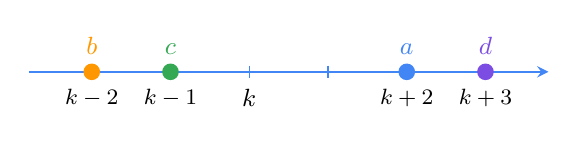
\begin{tikzpicture}[x=1cm,>=stealth]
\draw[->,thick,Navy] (-2.8,0)--(3.8,0);
\foreach \i in {-2,...,3}{\draw[Navy] (\i,0.08)--(\i,-0.08);}
\node[below,font=\small] at (0,-0.1){$k$};
\foreach \i/\l/\c in {-2/b/tmOrange,-1/c/tmGreen,2/a/tmBlue,3/d/tmPurple}{\fill[\c] (\i,0) circle (3pt); \node[above,font=\small\bfseries,text=\c] at (\i,0.1){$\l$};}
\node[below,font=\footnotesize] at (-2,-0.1){$k-2$}; \node[below,font=\footnotesize] at (-1,-0.1){$k-1$};
\node[below,font=\footnotesize] at (2,-0.1){$k+2$}; \node[below,font=\footnotesize] at (3,-0.1){$k+3$};
\end{tikzpicture}\end{center}

\textbf{3. Logical reasoning about order.} For sentences like ``An owns more cats than Bình'', translate them into symbols ($A>B$),
write down all the conditions and link them with the transitive property. A statement that ``\emph{must be true}'' has to be true in
\emph{every} situation that fits the problem; a single counter-example is enough to reject it.
\end{knowbox}

\begin{tipbox}
\emph{A reasoning example.} An is taller than Bình; Chi is shorter than Bình; Dũng is taller than Chi. Who is the shortest?
In symbols: $A>B$, \ $B>C$, \ $D>C$. From $A>B>C$ and $D>C$ we see that $A$, $B$ and $D$ are all taller than $C$: \textbf{Chi is the shortest}.
But we do \emph{not} know whether Dũng is taller or shorter than An (for instance, if An is $1.6$ m, Bình $1.5$ m and Chi $1.2$ m, then Dũng being $1.7$ m or $1.3$ m both fit all the conditions), so the statement ``Dũng is the tallest'' is \emph{not necessarily} true.
\end{tipbox}

\begin{warnbox}
Seeing that $a-2$ and $b+2$ are equal, many students conclude too quickly that ``$a$ is smaller because something is subtracted''. The opposite is true:
$a$ must \emph{lose} $2$ to equal $b$ \emph{plus} $2$, so $a$ is exactly $4$ more than $b$.
\end{warnbox}

\begin{parentbox}
Use real objects: ``If your bag loses $2$ marbles, it has the same number as my bag plus $2$ marbles. Which bag has more?''
Let your child check with marbles. A concrete picture keeps the child from being fooled by plus and minus signs.
\end{parentbox}

% ==========================================================================================
\needspace{6\baselineskip}\shead{Worked examples}

\begin{exbox}{Example 1 \ (Translating words and evaluating an expression)}
\textbf{a)} Evaluate the expression $A=2x^2-3x+1$ for $x=-2$.

\textbf{b)} Hoa has $50\,000$ dong in her piggy bank. Every week she puts in another $20\,000$ dong.
Write an expression for the amount in the piggy bank after $t$ weeks, then work out that amount after $6$ weeks.
\guide
\step{1}{Part a: substitute $x=-2$, remembering the brackets}
\[A=2\cdot(-2)^2-3\cdot(-2)+1.\]
\step{2}{Calculate in order: powers $\to$ multiplication $\to$ addition and subtraction}
$(-2)^2=(-2)\cdot(-2)=4$, so $2\cdot 4=8$. \ $3\cdot(-2)=-6$, so $-3\cdot(-2)=+6$. Hence $A=8+6+1=15$.
\step{3}{Part b: find the pattern with a small table}
\begin{center}
\begin{tabular}{|c|c|c|c|c|}
\hline
\rowcolor{tmBlue!10} Weeks & $0$ & $1$ & $2$ & $t$\\ \hline
Amount (dong) & $50\,000$ & $50\,000+20\,000$ & $50\,000+2\cdot 20\,000$ & $50\,000+20\,000t$\\ \hline
\end{tabular}
\end{center}
The starting amount stays the same; the added part is $20\,000$ times the number of weeks. Expression: $50\,000+20\,000t$ (dong).
\step{4}{Substitute $t=6$}
$50\,000+20\,000\cdot 6=50\,000+120\,000=170\,000$ (dong).
\begin{warnbox}Do not write $(50\,000+20\,000)\cdot t$: the starting amount is there only \emph{once}; it must not be multiplied by the number of weeks.\end{warnbox}
\ans{a) $A=15$;\ \ b) $50\,000+20\,000t$ dong; after $6$ weeks there are $170\,000$ dong.}
\end{exbox}

\begin{exbox}{Example 2 \ (Solving equations with the balance principle)}
Solve the equations:\quad \textbf{a)} $5x-7=2x+11$;\qquad \textbf{b)} $\dfrac{x}{12}=\dfrac{5}{4}$.
\guide
\step{1}{Part a: collect the terms with $x$ on the left}
Subtract $2x$ from both sides: $5x-2x-7=11$, that is, $3x-7=11$.
\step{2}{Collect the numbers on the right}
Add $7$ to both sides: $3x=11+7=18$.
\step{3}{Divide both sides by $3$}
$x=18\div 3=6$.
\verify{Left side: $5\cdot 6-7=30-7=23$. Right side: $2\cdot 6+11=12+11=23$. Both sides are equal.}
\step{4}{Part b: use a common denominator (or cross-multiply)}
We have $\dfrac{5}{4}=\dfrac{5\cdot 3}{4\cdot 3}=\dfrac{15}{12}$. The fractions $\dfrac{x}{12}$ and $\dfrac{15}{12}$ have the same denominator
and are equal, so $x=15$. (Cross-multiplying also works: $4x=12\cdot 5=60$, $x=60\div 4=15$.)
\begin{recallbox}$\dfrac{a}{b}=\dfrac{c}{d}$ exactly when $ad=bc$ ($b,d\neq 0$).\end{recallbox}
\ans{a) $x=6$;\ \ b) $x=15$.}
\end{exbox}

\begin{exbox}{Example 3 \ (Consecutive even numbers)}
The sum of four consecutive even numbers is $116$. Find the largest of the four numbers.
\guide
\step{1}{Choose an unknown}
Let the smallest even number be $n$ ($n$ is even). Consecutive even numbers differ by $2$, so the four numbers are
$n,\ n+2,\ n+4,\ n+6$.
\step{2}{Write an equation}
$n+(n+2)+(n+4)+(n+6)=116$, that is, $4n+12=116$.
\step{3}{Solve}
$4n=116-12=104$, \ $n=104\div 4=26$. The four numbers are $26,\ 28,\ 30,\ 32$.
\verify{$26+28+30+32=116$. Correct.}
\step{4}{Answer the actual question}
The question asks for the \emph{largest} number: it is $32$.
\begin{tipbox}Mental shortcut: the four numbers are equally spaced, so their average $116\div 4=29$ lies exactly halfway between the two middle numbers $28$ and $30$. The four numbers follow at once.\end{tipbox}
\ans{$32$}
\end{exbox}

\begin{exbox}{Example 4 \ (Weighing in pairs)}
Three friends, Mai, Lan and Hoa, step on a scale two at a time. Mai and Lan weigh $72$ kg; Mai and Hoa weigh $78$ kg;
Lan and Hoa weigh $80$ kg. How many kilograms does each girl weigh?
\guide
\step{1}{Add all three weighings}
In the three weighings, each girl is weighed exactly \emph{twice}:
$(M+L)+(M+H)+(L+H)=72+78+80=230$, that is, $2(M+L+H)=230$.
\step{2}{Total mass of the three girls}
$M+L+H=230\div 2=115$ (kg).
\step{3}{Find each girl: subtract the pair that does not contain her from the total}
Hoa $=115-(M+L)=115-72=43$ kg;\quad Lan $=115-(M+H)=115-78=37$ kg;\quad Mai $=115-(L+H)=115-80=35$ kg.
\begin{figC}
\foreach \y/\a/\b/\ca/\cb/\s in {0/Mai/Lan/tmBlue/tmOrange/72,-0.8/Mai/Hoa/tmBlue/tmGreen/78,-1.6/Lan/Hoa/tmOrange/tmGreen/80}{
  \node[draw=\ca!80!black,fill=\ca!15,rounded corners=2pt,minimum width=1.4cm] at (0,\y){\a};
  \node at (0.95,\y){$+$};
  \node[draw=\cb!80!black,fill=\cb!15,rounded corners=2pt,minimum width=1.4cm] at (1.9,\y){\b};
  \node[anchor=west] at (2.7,\y){$=\s$ kg};}
\end{figC}
\verify{$35+37=72$, \ $35+43=78$, \ $37+43=80$. All three weighings match.}
\ans{Mai $35$ kg, Lan $37$ kg, Hoa $43$ kg.}
\end{exbox}

\begin{exbox}{Example 5 \ (Arithmetic sequences)}
Consider the sequence $4,\ 7,\ 10,\ 13,\ \dots$ (each number is $3$ more than the one before).
\textbf{a)} Write an expression for the $n$-th term.\quad \textbf{b)} Find the $50$th term.\quad
\textbf{c)} Is $2026$ in the sequence? If so, which term is it?
\guide
\step{1}{The $n$-th term}
First term $a=4$, common difference $d=3$: the $n$-th term is $4+3(n-1)=4+3n-3=3n+1$.
\begin{recallbox}The $n$-th term of an arithmetic sequence $=a+(n-1)d$.\end{recallbox}
\step{2}{The $50$th term}
$3\cdot 50+1=151$.
\step{3}{Test the number $2026$}
We need a whole number $n$ with $3n+1=2026$, that is, $3n=2025$. Since $2025\div 3=675$ exactly, $n=675$.
\verify{$3\cdot 675+1=2025+1=2026$. Correct.}
\begin{warnbox}Do not forget to check that the division is exact. For instance, $2027$ is \emph{not} in the sequence because $2026$ is not divisible by $3$.\end{warnbox}
\ans{a) $3n+1$;\ \ b) $151$;\ \ c) yes, it is the $675$th term.}
\end{exbox}

\begin{exbox}{Example 6 \ (Motion, fractions and unit conversion)}
A train travels at a constant speed of $72$ km/h on a $360$ km route. It has already covered $\dfrac{2}{3}$ of the route.
How much longer (in hours and minutes) does the train need to reach its destination?
\guide
\step{1}{Distance already covered}
$\dfrac{2}{3}$ of $360$ km is $360\div 3\cdot 2=120\cdot 2=240$ km.
\step{2}{Distance left}
$360-240=120$ km. (Or: the remaining part is $1-\dfrac{2}{3}=\dfrac{1}{3}$ of the route, $360\div 3=120$ km.)
\begin{barfigC}
\blk{0}{5}{0}{0.55}{tmBlue}{covered 240 km}
\blk{5}{7.5}{0}{0.55}{tmOrange}{left 120 km}
\brcup{0}{7.5}{0.55}{360 km}
\end{barfigC}
\step{3}{Time left}
\begin{recallbox}$t=\dfrac{s}{v}$ (time $=$ distance $\div$ speed).\end{recallbox}
$t=120\div 72=\dfrac{120}{72}=\dfrac{5}{3}$ hours $=1\dfrac{2}{3}$ hours.
\step{4}{Convert to hours and minutes}
$\dfrac{2}{3}$ hour $=\dfrac{2}{3}\cdot 60=40$ minutes. So $t=1$ hour $40$ minutes.
\verify{In $1$ hour $40$ minutes $=\dfrac{5}{3}$ hours, the train covers $72\cdot\dfrac{5}{3}=24\cdot 5=120$ km, exactly the distance left.}
\ans{$1$ hour $40$ minutes.}
\end{exbox}

\begin{exbox}{Example 7 \ (A balance-scale problem)}
Both scales below are balanced. Identical shapes have equal weights.
\begin{center}
\aeaScale{\aeaSq}{\aeaTri\,\aeaCir}\hspace{1.2cm}\aeaScale{\aeaSq\,\aeaCir}{\aeaTri\,\aeaTri\,\aeaTri}
\end{center}
How many circles \aeaCir\ balance two squares \aeaSq\,\aeaSq?
\guide
\step{1}{Write each scale as an equation}
Let $S$, $T$, $C$ be the weights of a square, a triangle and a circle. Scale 1: $S=T+C$. \ Scale 2: $S+C=3T$.
\step{2}{Substitute scale 1 into scale 2}
On scale 2, replace the square by ``one triangle and one circle'' (allowed by scale 1):
$T+C+C=3T$.
\step{3}{Remove identical things from both pans}
Remove one triangle from each pan: $C+C=T+T$, that is, $2C=2T$, so $C=T$: a circle weighs the same as a triangle.
\step{4}{Answer}
$S=T+C=C+C=2C$, so $2S=4C$: two squares balance $4$ circles.
\verify{Try $C=T=1$, $S=2$: scale 1: $2=1+1$; scale 2: $2+1=3$. Both are correct.}
\ans{$4$ circles.}
\end{exbox}

\begin{exbox}{Example 8 \ (Ordering with the ``set it equal to $k$'' technique)}
The positive integers $a$, $b$, $c$ (all greater than $5$) satisfy\quad
$\dfrac{2}{a+3}=\dfrac{2}{b-1}=\dfrac{2}{c+5}$. Arrange $a$, $b$, $c$ in increasing order.
\guide
\step{1}{Equal fractions with the same numerator have equal denominators}
The three fractions all have numerator $2$ and are equal, so their denominators are equal: $a+3=b-1=c+5$.
\begin{recallbox}If $\dfrac{m}{p}=\dfrac{m}{q}$ with $m\neq 0$, then $p=q$.\end{recallbox}
\step{2}{Call the common value $k$}
$a+3=k\Rightarrow a=k-3$;\quad $b-1=k\Rightarrow b=k+1$;\quad $c+5=k\Rightarrow c=k-5$.
\step{3}{Compare with the reference point $k$}
$k-5<k-3<k+1$, so $c<a<b$.
\verify{Take $k=12$: $a=9$, $b=13$, $c=7$. Then $\dfrac{2}{12}=\dfrac{2}{12}=\dfrac{2}{12}$ and indeed $7<9<13$.}
\ans{$c<a<b$.}
\end{exbox}

% ==========================================================================================
\clearpage
\dividerbar{Core practice}

% ---------------------------------------------------------------- Problem 1
\begin{probbox}{1}{\relax}
Mr Tâm drives a car at a constant speed of $85$ km/h on a $510$ km trip. He has now covered exactly
half of the distance. How many more hours does he need to finish the trip?
\choices{$5$ hours}{$425$ hours}{$12$ hours}{$1.5$ hours}{$3$ hours}
\end{probbox}
\probsol{
\textbf{Understanding the problem.} \emph{Given:} speed $85$ km/h (constant), whole trip $510$ km, half already covered.
\emph{Find:} the time needed for the remaining part.
\step{1}{Work out the distance left}
Half has been covered, so exactly half is left: $510\div 2=255$ (km).
\begin{barfigC}
\blk{0}{3}{0}{0.55}{tmBlue}{covered 255 km}
\blk{3}{6}{0}{0.55}{tmOrange}{left 255 km}
\brcup{0}{6}{0.55}{510 km}
\end{barfigC}
\step{2}{Work out the time for the remaining distance}
\begin{recallbox}Distance $=$ speed $\times$ time, so time $=$ distance $\div$ speed ($t=\dfrac{s}{v}$).\end{recallbox}
$t=255\div 85=3$ (hours). (Mentally: $85\times 3=255$.)
\begin{warnbox}Calculating $510\div 85=6$ hours gives the time for the \emph{whole} trip, which does not answer the question. And $510-85=425$ is a meaningless calculation (km minus km/h); that is the trap in option (B).\end{warnbox}
\begin{tipbox}Another way: the whole trip takes $510\div 85=6$ hours; covering half the distance (at a constant speed) means half the time has passed, so $6\div 2=3$ hours are left.\end{tipbox}
\verify{In $3$ hours the car covers $85\times 3=255$ km, exactly the distance left.}
The result $3$ hours is option \textbf{(E)}.
\ans{(E) $3$ hours}
}

% ---------------------------------------------------------------- Problem 2
\begin{probbox}{2}{\relax}
In the diagram, the triangle has one side of length $14$ cm and two equal sides of length $12$ cm each; the rectangle has width
$8$ cm and length $x$ cm. The perimeter of the triangle equals the perimeter of the rectangle. Find $x$.
\begin{figC}
\draw[tmBlue,line width=1.1pt,fill=tmBlue!10] (0,2.6)--(2.8,2.6)--(1.4,1.2)--cycle;
\node[above] at (1.4,2.6){$14$ cm};
\node[right] at (2.15,1.9){$12$ cm};
\draw[tmBlue,line width=0.9pt] ($(0.7,1.9)+(-0.1,-0.1)$)--($(0.7,1.9)+(0.1,0.1)$);
\draw[tmBlue,line width=0.9pt] ($(2.1,1.9)+(-0.1,0.1)$)--($(2.1,1.9)+(0.1,-0.1)$);
\draw[tmOrange!85!black,line width=1.1pt,fill=tmOrange!12] (0.4,0)rectangle(2.4,0.9);
\node[right] at (2.4,0.45){$8$ cm};
\node[below] at (1.4,0){$x$ cm};
\end{figC}
\choices{$8$}{$10$}{$11$}{$14$}{$15$}
\end{probbox}
\probsol{
\textbf{Understanding the problem.} The triangle has sides $14$ cm, $12$ cm, $12$ cm (the small tick marks show that those two sides are equal).
The rectangle measures $x$ cm by $8$ cm. The two perimeters are equal. We must find $x$.
\step{1}{Work out the perimeter of the triangle}
\begin{recallbox}The perimeter of a triangle is the sum of its three sides. The perimeter of a rectangle is $2\times(\text{length}+\text{width})$.\end{recallbox}
Perimeter of the triangle: $14+12+12=38$ (cm).
\begin{warnbox}The number $12$ is written only once in the diagram, but there are \emph{two} sides of $12$ cm (marked as equal). Forgetting the third side gives $26$ cm and a wrong answer.\end{warnbox}
\step{2}{Write an equation}
The perimeter of the rectangle is $2(x+8)$. Setting the two perimeters equal: $2(x+8)=38$.
\step{3}{Solve the equation}
Divide both sides by $2$: $x+8=19$. Subtract $8$ from both sides: $x=19-8=11$.
\verify{An $11$ cm $\times$ $8$ cm rectangle has perimeter $11+8+11+8=38$ cm, the same as the triangle.}
The value $x=11$ is option \textbf{(C)}.
\begin{parentbox}You can illustrate this with a piece of string $38$ cm long: bend it into a $14$ -- $12$ -- $12$ triangle, then reshape it into a rectangle with an $8$ cm side. Your child will see that the ``perimeter'' is just the length of the string, which does not change when the shape changes.\end{parentbox}
\ans{(C) $11$}
}

% ---------------------------------------------------------------- Problem 3
\begin{probbox}{3}{\relax}
Let $x=3$. Which of the following equations is true?
\choices{$2x=5$}{$3x-1=8$}{$x+5=3$}{$7-x=2$}{$6+2x=14$}
\end{probbox}
\probsol{
\textbf{Understanding the problem.} Substitute $x=3$ into the left side of each equation, work it out, and compare with the right side. Only one equation is true.
\begin{recallbox}To evaluate an expression, replace the letter by the number and calculate in order: multiplication and division first, then addition and subtraction.\end{recallbox}
\step{1}{Check each option in turn}
\begin{center}
\begin{tabular}{|c|l|c|c|}
\hline
\rowcolor{tmBlue!10} Option & Left side with $x=3$ & Right side & True/False\\ \hline
(A) & $2x=2\cdot 3=6$ & $5$ & False\\ \hline
(B) & $3x-1=3\cdot 3-1=9-1=8$ & $8$ & \textbf{True}\\ \hline
(C) & $x+5=3+5=8$ & $3$ & False\\ \hline
(D) & $7-x=7-3=4$ & $2$ & False\\ \hline
(E) & $6+2x=6+2\cdot 3=6+6=12$ & $14$ & False\\ \hline
\end{tabular}
\end{center}
\begin{warnbox}In (E), working in the wrong order, $(6+2)\cdot 3=24$, or reading $2x$ as ``$23$'' leads to mistakes. Multiply first, then add: $6+2\cdot 3=12$.\end{warnbox}
\step{2}{Conclusion}
Only the equation in (B) is true: $3\cdot 3-1=8$. So the answer is \textbf{(B)}.
\ans{(B) $3x-1=8$}
}

% ---------------------------------------------------------------- Problem 4
\begin{probbox}{4}{\relax}
The sum of three consecutive integers is $153$. The largest of the three integers is
\choices{$52$}{$50$}{$53$}{$54$}{$51$}
\end{probbox}
\probsol{
\textbf{Understanding the problem.} Three consecutive integers stand next to each other on the number line and differ by $1$ (for example $7,8,9$). Their sum is $153$. We want the \emph{largest} one.
\step{1}{Choose an unknown: let the middle number be $n$}
The three numbers are $n-1$, \ $n$, \ $n+1$.
\step{2}{Write an equation}
$(n-1)+n+(n+1)=153$. On the left, $-1$ and $+1$ cancel, leaving $3n=153$.
\step{3}{Solve}
$n=153\div 3=51$. The three numbers are $50$, $51$, $52$.
\begin{recallbox}For three consecutive integers, the middle number equals the sum divided by $3$ (the middle number is the average).\end{recallbox}
\begin{proofbox}Another way, letting the smallest number be $m$: $m+(m+1)+(m+2)=3m+3=153$, so $3m=150$, $m=50$. The same three numbers $50,51,52$.\end{proofbox}
\begin{tipbox}Multiple-choice shortcut: the largest number must be a little more than the average $153\div 3=51$; try $50+51+52=153$ straight away.\end{tipbox}
\verify{$50+51+52=153$. Correct.}
\step{4}{Answer the actual question}
The largest number is $52$, which is option \textbf{(A)}.
\begin{warnbox}Option (E) $51$ is the \emph{middle} number and option (B) $50$ is the \emph{smallest} number. Read the question carefully so you do not choose the wrong one.\end{warnbox}
\ans{(A) $52$}
}

% ---------------------------------------------------------------- Problem 5
\begin{probbox}{5}{\relax}
One scoop of fish food can feed $8$ goldfish. How many goldfish can $4$ such scoops of fish food feed?
\choices{$12$}{$16$}{$8$}{$64$}{$32$}
\end{probbox}
\probsol{
\textbf{Understanding the problem.} $1$ scoop $\to$ $8$ fish. Asked: $4$ scoops $\to$ ? fish.
When the number of scoops is multiplied by some number, the number of fish fed is multiplied by the same number (the quantities are directly proportional).
\begin{recallbox}If $y$ is directly proportional to $x$ with constant $k$, then $y=k\cdot x$. Here $k=8$ (fish per scoop), so number of fish $=8\times$ number of scoops.\end{recallbox}
\step{1}{Draw a diagram}
\begin{barfigC}
\blk{0}{1.5}{0}{0.55}{tmGreen}{8 fish}
\blk{1.5}{3}{0}{0.55}{tmGreen}{8 fish}
\blk{3}{4.5}{0}{0.55}{tmGreen}{8 fish}
\blk{4.5}{6}{0}{0.55}{tmGreen}{8 fish}
\brcup{0}{6}{0.55}{4 scoops}
\end{barfigC}
\step{2}{Calculate}
$4\times 8=32$ (fish).
\begin{warnbox}Option (A) $12$ is $8+4$ (adding instead of multiplying), and option (D) $64$ is $8\times 8$. Each extra scoop feeds \emph{$8$ more fish}, so multiply $8$ by the number of scoops.\end{warnbox}
\verify{$32\div 4=8$: exactly $8$ fish per scoop.}
So the answer is \textbf{(E)}.
\ans{(E) $32$}
}

% ---------------------------------------------------------------- Problem 6
\begin{probbox}{6}{\relax}
If $x=4$ and $y=3x$, the value of $y$ is
\choices{$12$}{$24$}{$7$}{$81$}{$4$}
\end{probbox}
\probsol{
\textbf{Understanding the problem.} We know $x=4$. The expression $y=3x$ means ``$y$ equals $3$ times $x$''. We must find $y$.
\begin{recallbox}$3x$ is short for $3\cdot x$ (between a number and a letter we leave out the multiplication sign).\end{recallbox}
\step{1}{Substitute $x=4$}
$y=3\cdot x=3\cdot 4=12$.
\begin{warnbox}Do not read $3x$ as ``$34$'' (joining the digits); it is not $3+4=7$ (option C) or $3^4=81$ (option D) either.\end{warnbox}
\begin{tipbox}Read $y=3x$ in words: ``$y$ is three times $x$''. Three times $4$ is $12$.\end{tipbox}
\verify{$12\div 3=4=x$. Correct.}
So the answer is \textbf{(A)}.
\ans{(A) $12$}
}

% ---------------------------------------------------------------- Problem 7
\begin{probbox}{7}{\relax}
Each bus ride costs Lan $6\,750$ dong, while Minh pays $9\,000$ dong per ride (they use different routes).
If each of them rides the bus $20$ times, how much less does Lan pay than Minh in total?
\choicesII{$75\,000$ dong}{$30\,000$ dong}{$45\,000$ dong}{$135\,000$ dong}{$180\,000$ dong}
\end{probbox}
\probsol{
\textbf{Understanding the problem.} Per ride: Lan $6\,750$ dong, Minh $9\,000$ dong. Each rides $20$ times. We want the \emph{difference} after $20$ rides.
\step{1}{Method 1 -- Work out each total and subtract}
Lan pays: $20\times 6\,750=135\,000$ (dong).\quad Minh pays: $20\times 9\,000=180\,000$ (dong).\\
Difference: $180\,000-135\,000=45\,000$ (dong).
\step{2}{Method 2 -- Work out the difference per ride and multiply (quicker)}
Each ride, Lan pays less than Minh by: $9\,000-6\,750=2\,250$ (dong).\\
After $20$ rides: $20\times 2\,250=45\,000$ (dong).
\begin{recallbox}The distributive law: $20\times 9\,000-20\times 6\,750=20\times(9\,000-6\,750)$. That is why both methods always agree.\end{recallbox}
\begin{warnbox}Option (D) $135\,000$ dong is \emph{Lan's total} and option (E) $180\,000$ dong is \emph{Minh's total}. The question asks how much \emph{less}, which is the difference.\end{warnbox}
\verify{$135\,000+45\,000=180\,000$. Correct.}
So the answer is \textbf{(C)}.
\ans{(C) $45\,000$ dong}
}

% ---------------------------------------------------------------- Problem 8
\begin{probbox}{8}{\relax}
Which expression produces the values in the second row of the table, given the values of $n$ in the first row?
\begin{center}
\begin{tabular}{|c|c|c|c|c|c|}
\hline
\rowcolor{tmBlue!10} $n$ & $1$ & $2$ & $3$ & $4$ & $5$\\ \hline
Value & $1$ & $3$ & $5$ & $7$ & $9$\\ \hline
\end{tabular}
\end{center}
\choices{$3n-2$}{$2(n-1)$}{$n+4$}{$2n$}{$2n-1$}
\end{probbox}
\probsol{
\textbf{Understanding the problem.} We need an expression in $n$ which gives $1,3,5,7,9$ when $n=1,2,3,4,5$.
\step{1}{Find the pattern in the row of values}
Each time $n$ increases by $1$, the value increases by $2$ ($1\to 3\to 5\to 7\to 9$). So the expression has the form $2n+b$.
\begin{recallbox}If the value always increases by $d$ when $n$ increases by $1$, the expression has the form $d\cdot n+b$; find $b$ by substituting $n=1$.\end{recallbox}
\step{2}{Find $b$}
Substitute $n=1$: $2\cdot 1+b=1$, so $b=1-2=-1$. The expression is $2n-1$.
\step{3}{Check the whole table and rule out the other options}
\begin{center}
\begin{tabular}{|c|c|c|c|c|c|c|}
\hline
\rowcolor{tmBlue!10} $n$ & $1$ & $2$ & $3$ & $4$ & $5$ & Verdict\\ \hline
(A) $3n-2$ & $1$ & $4$ & & & & fails at $n=2$\\ \hline
(B) $2(n-1)$ & $0$ & & & & & fails at $n=1$\\ \hline
(C) $n+4$ & $5$ & & & & & fails at $n=1$\\ \hline
(D) $2n$ & $2$ & & & & & fails at $n=1$\\ \hline
(E) $2n-1$ & $1$ & $3$ & $5$ & $7$ & $9$ & \textbf{fits the whole table}\\ \hline
\end{tabular}
\end{center}
\begin{warnbox}Option (A) $3n-2$ also gives $1$ when $n=1$. If you only test the first column, you cannot decide between (A) and (E). Test other columns too.\end{warnbox}
\verify{$2n-1$ for $n=1,2,3,4,5$: $1,3,5,7,9$. It matches the whole table.}
So the answer is \textbf{(E)}.
\ans{(E) $2n-1$}
}

% ---------------------------------------------------------------- Problem 9
\begin{probbox}{9}{\relax}
When two numbers are added, the result is $-26$. One of the numbers is $11$. The other number is
\choices{$-37$}{$37$}{$-15$}{$15$}{$-48$}
\end{probbox}
\probsol{
\textbf{Understanding the problem.} Call the unknown number $x$. We are told that $x+11=-26$. We must find $x$.
\step{1}{Write an equation}
$x+11=-26$.
\step{2}{Solve with the balance principle}
Subtract $11$ from both sides: $x=-26-11$.
\begin{recallbox}Subtracting a number means adding its opposite: $-26-11=-26+(-11)$. Adding two negative numbers: add the sizes and keep the ``$-$'' sign: $-(26+11)=-37$.\end{recallbox}
So $x=-37$.
\begin{center}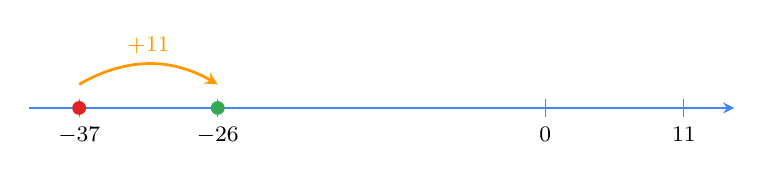
\begin{tikzpicture}[x=0.16cm,>=stealth]
\draw[->,thick,Navy] (-41,0)--(15,0);
\foreach \i in {-37,-26,0,11}{\draw[Navy] (\i,0.12)--(\i,-0.12); \node[below,font=\footnotesize] at (\i,-0.12){$\i$};}
\fill[AnsRed] (-37,0) circle (2.5pt); \fill[tmGreen] (-26,0) circle (2.5pt);
\draw[->,tmOrange,line width=1pt] (-37,0.3) to[bend left=30] node[above,font=\footnotesize]{$+11$} (-26,0.3);
\end{tikzpicture}\end{center}
On the number line: starting from $-37$ and moving $11$ steps to the right, we arrive at $-26$.
\begin{warnbox}Forgetting to change the sign when moving a term across, and writing $x=-26+11=-15$, is wrong (option C). Check: $-15+11=-4\neq -26$.\end{warnbox}
\begin{parentbox}You can explain it with a story about owing money: ``After someone gives you $11$ thousand, you still owe $26$ thousand. How much did you owe at first?'' At first you owed more: $26+11=37$ thousand, that is, $-37$.\end{parentbox}
\verify{$(-37)+11=-26$. Correct.}
So the answer is \textbf{(A)}.
\ans{(A) $-37$}
}

% ---------------------------------------------------------------- Problem 10
\begin{probbox}{10}{\relax}
Mr Hùng has $10\,000\,000$ dong, all in $50\,000$ dong notes. How many notes does he have?
\choices{$1\,000$}{$200$}{$1\,250$}{$500$}{$2\,000$}
\end{probbox}
\probsol{
\textbf{Understanding the problem.} The total amount is $10\,000\,000$ dong (ten million dong). Each note is worth $50\,000$ dong. We must find the number of notes.
\begin{recallbox}Number of notes $=$ total amount $\div$ value of one note.\end{recallbox}
\step{1}{Set up the division}
Number of notes $=10\,000\,000\div 50\,000$.
\step{2}{Simplify by removing zeros}
Remove four zeros from both numbers (that is, divide both by $10\,000$; the quotient does not change): $10\,000\,000\div 50\,000=1\,000\div 5=200$.
\step{3}{Another way of thinking}
$2$ notes of $50\,000$ dong make $100\,000$ dong. Ten million dong is $100$ times $100\,000$ dong, so there are $100\times 2=200$ notes.
\verify{$200\times 50\,000=10\,000\,000$ dong. Correct.}
\begin{warnbox}Miscounting the zeros is a very common mistake. Write numbers with a space between groups of three digits ($10\,000\,000$) to count accurately.\end{warnbox}
So the answer is \textbf{(B)}.
\begin{parentbox}If you have real banknotes at home, let your child count $10$ notes of $50\,000$ dong ($500\,000$ dong), then ask: how many such bundles make $10$ million? ($20$ bundles, that is, $200$ notes.)\end{parentbox}
\ans{(B) $200$}
}

% ---------------------------------------------------------------- Problem 11
\begin{probbox}{11}{\relax}
The product $60\times 60\times 24\times 7$ equals
\choicesL{the number of minutes in seven weeks}{the number of hours in sixty days}{the number of seconds in seven hours}{the number of seconds in one week}{the number of minutes in twenty-four weeks}
\end{probbox}
\probsol{
\textbf{Understanding the problem.} There is no need to multiply the product out. Read each factor as one step of a time-unit conversion.
\begin{recallbox}$1$ week $=7$ days;\ \ $1$ day $=24$ hours;\ \ $1$ hour $=60$ minutes;\ \ $1$ minute $=60$ seconds.\end{recallbox}
\step{1}{Read the product from right to left}
\begin{itemize}[leftmargin=1.4em,itemsep=1pt,topsep=1pt]
\item $7$ is the number of days in \textbf{one week};
\item $24\times 7$ is the number of hours in one week;
\item $60\times 24\times 7$ is the number of minutes in one week;
\item $60\times 60\times 24\times 7$ is the number of \textbf{seconds} in one week.
\end{itemize}
\step{2}{Check the other options by writing their products}
\begin{center}
\begin{tabular}{|c|l|r|}
\hline
\rowcolor{tmBlue!10} Option & Expression & Value\\ \hline
(A) minutes in $7$ weeks & $60\times 24\times 7\times 7$ & $70\,560$\\ \hline
(B) hours in $60$ days & $24\times 60$ & $1\,440$\\ \hline
(C) seconds in $7$ hours & $60\times 60\times 7$ & $25\,200$\\ \hline
(D) seconds in $1$ week & $60\times 60\times 24\times 7$ & $604\,800$\\ \hline
(E) minutes in $24$ weeks & $60\times 24\times 7\times 24$ & $241\,920$\\ \hline
\end{tabular}
\end{center}
Only option (D) has exactly the product $60\times 60\times 24\times 7=604\,800$.
\begin{warnbox}Seeing the numbers $60$, $24$, $7$ in the wording, many students rush to choose (A) or (E). Match \emph{every} conversion step: (A) is missing one factor $60$ and has an extra factor $7$.\end{warnbox}
So the answer is \textbf{(D)}.
\ans{(D) the number of seconds in one week}
}

% ---------------------------------------------------------------- Problem 12
\begin{probbox}{12}{\stars{1}}
Each of $a$, $b$, $c$, $d$ is a positive integer greater than $3$, and
\[\frac{1}{a-2}=\frac{1}{b+2}=\frac{1}{c+1}=\frac{1}{d-3}.\]
Which ordering of these four numbers is correct?
\choicesII{$a<b<c<d$}{$c<b<a<d$}{$b<a<c<d$}{$d<a<c<b$}{$b<c<a<d$}
\end{probbox}
\probsol{
\textbf{Understanding the problem.} Four fractions with the same numerator $1$ are equal. We must compare $a,b,c,d$.
(The condition ``greater than $3$'' makes sure all the denominators are non-zero, so the fractions make sense.)
\step{1}{Equal fractions with the same numerator have equal denominators}
\begin{recallbox}If $\dfrac{1}{p}=\dfrac{1}{q}$, then $p=q$ (cross-multiply: $1\cdot q=1\cdot p$).\end{recallbox}
Therefore: $a-2=b+2=c+1=d-3$.
\step{2}{Call the common value $k$ and write each number in terms of $k$}
$a-2=k\Rightarrow a=k+2$;\quad $b+2=k\Rightarrow b=k-2$;\quad $c+1=k\Rightarrow c=k-1$;\quad $d-3=k\Rightarrow d=k+3$.
\step{3}{Compare with the same reference point $k$}
The ``extras'' are $-2$ (for $b$), $-1$ (for $c$), $+2$ (for $a$), $+3$ (for $d$). Since $-2<-1<2<3$,
\[k-2<k-1<k+2<k+3,\quad\text{that is,}\quad b<c<a<d.\]
\begin{center}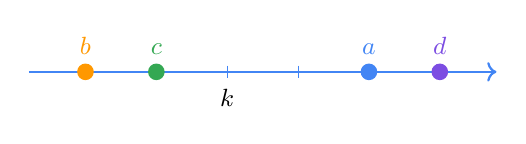
\begin{tikzpicture}[x=0.9cm]
\draw[->,thick,Navy] (-2.8,0)--(3.8,0);
\foreach \i in {-2,...,3}{\draw[Navy] (\i,0.08)--(\i,-0.08);}
\node[below,font=\small] at (0,-0.1){$k$};
\foreach \i/\l/\c in {-2/b/tmOrange,-1/c/tmGreen,2/a/tmBlue,3/d/tmPurple}{\fill[\c] (\i,0) circle (3pt); \node[above,font=\small\bfseries,text=\c] at (\i,0.1){$\l$};}
\end{tikzpicture}\end{center}
\begin{warnbox}Seeing the minus sign in ``$a-2$'', many students think $a$ is small. But $a$ has to \emph{lose} $2$ to equal $k$, so $a$ is bigger than $k$. On the other hand, $b$ has to \emph{gain} $2$ to equal $k$, so $b$ is smaller than $k$.\end{warnbox}
\verify{Try $k=6$ (so that all four numbers are greater than $3$): $a=8$, $b=4$, $c=5$, $d=9$. Then $\dfrac{1}{8-2}=\dfrac{1}{4+2}=\dfrac{1}{5+1}=\dfrac{1}{9-3}=\dfrac{1}{6}$ and indeed $4<5<8<9$, that is, $b<c<a<d$.}
The ordering $b<c<a<d$ is option \textbf{(E)}.
\ans{(E) $b<c<a<d$}
}

% ---------------------------------------------------------------- Problem 13
\begin{probbox}{13}{\relax}
A rectangle has length $x$ and width $y$. A triangle has base $16$ and corresponding height $x$.
If the area of the rectangle equals the area of the triangle, then the value of $y$ is
\choices{$16$}{$4$}{$8$}{$12$}{$32$}
\end{probbox}
\probsol{
\textbf{Understanding the problem.} Rectangle: length $x$, width $y$. Triangle: base $16$, height $x$. The two areas are equal. Find $y$
(note: $x$ is not given, but we will see that $x$ ``disappears'').
\begin{figC}
\draw[tmBlue,line width=1pt,fill=tmBlue!10] (0,0) rectangle (2.4,1.4);
\node[below] at (1.2,0){$x$}; \node[left] at (0,0.7){$y$};
\draw[tmOrange!85!black,line width=1pt,fill=tmOrange!12] (3.6,0)--(7.6,0)--(4.6,2.4)--cycle;
\draw[dashed,Slate] (4.6,2.4)--(4.6,0); \draw[Slate] (4.6,0.18)--(4.78,0.18)--(4.78,0);
\node[below] at (5.6,0){$16$}; \node[left,font=\small] at (4.6,1.1){$x$};
\end{figC}
\step{1}{Write the two area formulas}
\begin{recallbox}Area of a rectangle $=$ length $\times$ width. Area of a triangle $=\dfrac{\text{base}\times\text{height}}{2}$.\end{recallbox}
Rectangle: $A_1=x\cdot y=xy$.\quad Triangle: $A_2=\dfrac{16\cdot x}{2}=8x$.
\step{2}{Write an equation and solve}
$xy=8x$. Since $x$ is a length, $x>0$; dividing both sides by $x$: $y=8$.
\begin{proofbox}You can also see it without dividing: $x\cdot y$ and $x\cdot 8$ are ``$x$ groups of $y$'' and ``$x$ groups of $8$''. If the products are equal with the same number of groups $x\neq 0$, each group must be the same: $y=8$.\end{proofbox}
\begin{warnbox}Forgetting to halve when finding the area of the triangle leads to $y=16$ (option A).\end{warnbox}
\verify{Try $x=5$: rectangle $5\times 8=40$; triangle $\dfrac{16\cdot 5}{2}=40$. Equal. (It works for any $x$.)}
So the answer is \textbf{(C)}.
\ans{(C) $8$}
}

% ---------------------------------------------------------------- Problem 14
\begin{probbox}{14}{\relax}
The symbol \aeaBox{3}{4}{5}{6} is evaluated as $3\times 6+4\times 5=38$. If \aeaBox{2}{6}{1}{\ } is evaluated as $16$,
then the number that should be placed in the empty space is
\choices{$1$}{$2$}{$3$}{$4$}{$5$}
\end{probbox}
\probsol{
\textbf{Understanding the problem.} First we must understand the rule from the given example, then apply it to the box with the unknown number.
\step{1}{Find the rule}
In \aeaBox{3}{4}{5}{6}: $3$ (top left) times $6$ (bottom right), plus $4$ (top right) times $5$ (bottom left): $3\times 6+4\times 5=18+20=38$.
That is: \emph{multiply the two numbers on each diagonal, then add}. In general, \aeaBox{a}{b}{c}{d} $=a\times d+b\times c$.
\step{2}{Name the empty space and write an equation}
Let the number in the empty space (bottom right) be $x$. By the rule: \aeaBox{2}{6}{1}{x} $=2\times x+6\times 1=2x+6$.
We are told the value is $16$: $2x+6=16$.
\step{3}{Solve}
Subtract $6$ from both sides: $2x=10$. Divide both sides by $2$: $x=5$.
\verify{$2\times 5+6\times 1=10+6=16$. Correct.}
\begin{warnbox}Do not pair the wrong numbers: $2\times 6+1\times x$ (multiplying along rows) breaks the rule; that way you would get $x=4$ (option D). Check the rule against the example $38$ before using it.\end{warnbox}
So the answer is \textbf{(E)}.
\begin{parentbox}Together with your child, ``invent'' a new symbol (for example, multiply along the rows and then subtract) and quiz each other. The important habit is always to test a rule on the given example before using it.\end{parentbox}
\ans{(E) $5$}
}

% ---------------------------------------------------------------- Problem 15
\begin{probbox}{15}{\relax}
Three pumpkins are weighed two at a time in all possible ways. The weights of the pairs are $12$ kg, $13$ kg and $15$ kg.
How much does the lightest pumpkin weigh?
\choices{$4$ kg}{$5$ kg}{$6$ kg}{$7$ kg}{$8$ kg}
\end{probbox}
\probsol{
\textbf{Understanding the problem.} Three pumpkins can be paired in exactly $3$ ways. Let their weights from lightest to heaviest be $a\le b\le c$ (kg).
The lightest pair is the two lightest pumpkins, and the heaviest pair is the two heaviest pumpkins:
$a+b=12$, \ $a+c=13$, \ $b+c=15$.
\step{1}{Add all three pairs}
Each pumpkin appears in exactly \emph{two} pairs: $(a+b)+(a+c)+(b+c)=12+13+15=40$, that is, $2(a+b+c)=40$.
\begin{recallbox}Three objects weighed in pairs: the total of the three objects is half of the sum of the results.\end{recallbox}
\step{2}{Total weight of the three pumpkins}
$a+b+c=40\div 2=20$ (kg).
\step{3}{Find the lightest pumpkin}
The lightest pumpkin $a$ is the one that is \emph{not} in the heaviest pair ($b+c=15$):
$a=(a+b+c)-(b+c)=20-15=5$ (kg).
(Similarly: $b=20-13=7$ kg, \ $c=20-12=8$ kg.)
\begin{barfigC}
\blk{0}{1.25}{0}{0.5}{tmGreen}{a}
\blk{1.25}{3}{0}{0.5}{tmOrange}{b}
\brcup{0}{3}{0.5}{12 kg}
\blk{0}{1.25}{-0.9}{0.5}{tmGreen}{a}
\blk{1.25}{3.25}{-0.9}{0.5}{tmPurple}{c}
\brcdn{0}{3.25}{-1.35}{13 kg}
\end{barfigC}
\verify{$5+7=12$, \ $5+8=13$, \ $7+8=15$. All three pairs are correct.}
\begin{warnbox}Do not take $12\div 2=6$ kg and assume each pumpkin in the lightest pair weighs $6$ kg: the two pumpkins in a pair need not weigh the same. Option (E) $8$ kg is the \emph{heaviest} pumpkin.\end{warnbox}
The lightest pumpkin weighs $5$ kg, which is option \textbf{(B)}.
\begin{parentbox}Let your child take three objects at home and a scale: weigh them in pairs, add the three results and halve, then compare with putting all three on the scale together. Your child will see for themselves why we divide by $2$.\end{parentbox}
\ans{(B) $5$ kg}
}

% ---------------- part b ----------------
% ===== Topic 1, part b (EN): problems 16-30 =====
% helper shapes for the balance-scale problems (topic-specific prefix \ae...)
% \aeShp{code}{x}{y}: draw shape (T triangle, C circle, S square, D diamond, Q question mark) with lower-left corner at (x,y)
\providecommand{\aeShp}[3]{%
  \if#1T\draw[tmBlue!80!black,line width=0.8pt,fill=tmBlue!18] (#2,#3)--(#2+0.34,#3)--(#2+0.17,#3+0.3)--cycle;\fi
  \if#1C\draw[tmOrange!85!black,line width=0.8pt,fill=tmOrange!22] (#2+0.15,#3+0.15) circle (0.15);\fi
  \if#1S\draw[tmGreen!80!black,line width=0.8pt,fill=tmGreen!18] (#2,#3) rectangle (#2+0.3,#3+0.3);\fi
  \if#1D\draw[tmPurple!85!black,line width=0.8pt,fill=tmPurple!18] (#2+0.13,#3)--(#2+0.26,#3+0.16)--(#2+0.13,#3+0.32)--(#2,#3+0.16)--cycle;\fi
  \if#1Q\node[font=\Large\bfseries,text=Ink,inner sep=0pt,anchor=south] at (#2+0.15,#3) {?};\fi}
\providecommand{\aeTri}{\tikz[baseline=0pt]{\aeShp{T}{0}{0}}}
\providecommand{\aeCir}{\tikz[baseline=0pt]{\aeShp{C}{0}{0}}}
\providecommand{\aeSq}{\tikz[baseline=0pt]{\aeShp{S}{0}{0}}}
\providecommand{\aeDia}{\tikz[baseline=0pt]{\aeShp{D}{0}{0}}}
% \aeRow{list}{xcentre}{y}: a row of shapes (e.g. {T,C}) centred at xcentre, standing on height y
\providecommand{\aeRow}[3]{%
  \foreach \aeS [count=\aeI] in {#1}{\xdef\aeN{\aeI}}%
  \foreach \aeS [count=\aeI] in {#1}{\aeShp{\aeS}{#2-0.19*\aeN+0.38*\aeI-0.36}{#3+0.03}}}
% \aeScale{x}{y}{left list}{right list}: a balanced scale centred at (x,y)
\providecommand{\aeScale}[4]{\begin{scope}[shift={(#1,#2)}]
  \draw[Ink,line width=1pt] (-1.9,0.55)--(-0.5,0.55) (-1.2,0.55)--(-1.2,0.25)--(1.2,0.25)--(1.2,0.55) (0.5,0.55)--(1.9,0.55);
  \draw[Ink,line width=0.9pt,fill=Ink!12] (-0.2,-0.12)--(0,0.25)--(0.2,-0.12)--cycle;
  \aeRow{#3}{-1.2}{0.55}\aeRow{#4}{1.2}{0.55}
\end{scope}}

% ------------------------------------------------------------------ 16
\begin{probbox}{16}{\relax}
Hồng is learning to save money. Today she has $120$ thousand dong in her savings account. From now on, every time she makes a deposit she will add exactly $30$ thousand dong. If Hồng makes $m$ such deposits, which expression correctly gives the amount of money (in thousands of dong) in her account?
\choices{$120+m$}{$30m$}{$30+120m$}{$150m$}{$120+30m$}
\end{probbox}
\probsol{
\textbf{Analysis.} Given: at the start there are $120$ thousand dong; each deposit adds $30$ thousand dong; there are $m$ deposits. Find: an algebraic expression for the total after $m$ deposits.

\step{1}{Try a few concrete values of $m$ to see the pattern}
\begin{center}
\begin{tabular}{|c|c|c|}
\hline
\rowcolor{tmBlue!10}\textbf{Deposits} & \textbf{Money added} & \textbf{Total (thousand dong)}\\ \hline
$0$ & $0$ & $120$\\ \hline
$1$ & $30$ & $120+30=150$\\ \hline
$2$ & $30+30=30\cdot 2=60$ & $120+60=180$\\ \hline
$3$ & $30\cdot 3=90$ & $120+90=210$\\ \hline
$m$ & $30\cdot m=30m$ & $120+30m$\\ \hline
\end{tabular}
\end{center}

\step{2}{Write the expression}
The money \emph{added} after $m$ deposits is $m$ times $30$, that is $30m$. Adding the $120$ already in the account gives
\[ \text{Total} = 120 + 30m \ \text{(thousand dong)}. \]
\begin{recallbox}$30m$ means $30\cdot m$ (we may leave out the multiplication sign between a number and a letter). Adding a number $a$ to itself $m$ times gives $a\cdot m$.\end{recallbox}

\step{3}{Rule out the wrong options}
\begin{itemize}[leftmargin=1.3em,itemsep=1pt]
\item (A) $120+m$: adds only $1$ thousand each time -- wrong.
\item (B) $30m$: forgets the $120$ thousand already there. For $m=0$ it gives $0$ -- wrong.
\item (C) $30+120m$: swaps the roles of the two numbers. For $m=1$ it gives $150$ (the same!), but for $m=2$ it gives $270\ne 180$ -- wrong.
\item (D) $150m$: for $m=2$ it gives $300\ne 180$ -- wrong.
\end{itemize}
\begin{warnbox}Testing only \emph{one} value, $m=1$, is not enough: (C), (D) and (E) all give $150$. Also try $m=0$ or $m=2$ to tell them apart.\end{warnbox}
\verify{For $m=3$: $120+30\cdot 3=210$, exactly as in the table of Step 1.}
So the answer is \textbf{(E)}.
\ans{(E) $120+30m$}
}

% ------------------------------------------------------------------ 17
\begin{probbox}{17}{\relax}
All four scales below are balanced. Identical shapes have equal masses. One possible replacement for the ``?'' that keeps the fourth scale balanced is
\begin{figC}
\aeScale{0}{1.6}{T,C}{S}
\aeScale{4.6}{1.6}{T}{D,C}
\aeScale{0}{0}{D,T}{C,S}
\aeScale{4.6}{0}{C,D,T}{Q}
\node[font=\footnotesize\bfseries,text=Slate] at (-2.25,2.45) {1};
\node[font=\footnotesize\bfseries,text=Slate] at (2.35,2.45) {2};
\node[font=\footnotesize\bfseries,text=Slate] at (-2.25,0.85) {3};
\node[font=\footnotesize\bfseries,text=Slate] at (2.35,0.85) {4};
\end{figC}
\choices{\aeTri\,\aeSq}{\aeDia\,\aeTri}{\aeCir\,\aeSq}{\aeSq\,\aeDia}{\aeTri\,\aeCir}
\end{probbox}
\probsol{
\textbf{Analysis.} Each balanced scale gives an \emph{equation}: the total mass on the left pan equals the total mass on the right pan. We write the shapes straight into the equations (each shape stands for its mass):
\[
\text{Scale 1: } \aeTri+\aeCir=\aeSq,\qquad
\text{Scale 2: } \aeTri=\aeDia+\aeCir,\qquad
\text{Scale 3: } \aeDia+\aeTri=\aeCir+\aeSq.
\]
Find: the right pan of scale 4 must weigh the same as $\aeCir+\aeDia+\aeTri$. Idea: convert every shape into one common ``unit'', namely \aeCir.
\begin{recallbox}If a scale is balanced, then \emph{replacing} an object by objects of the same mass, or \emph{removing} identical objects from both pans, keeps it balanced. This is exactly the property of equations: $a=b \Rightarrow a+c=b+c$ and $a-c=b-c$.\end{recallbox}

\step{1}{Use scale 2 to replace \aeTri\ in scale 1}
By scale 2, $\aeTri=\aeDia+\aeCir$. Substituting into scale 1:
\[ \aeSq=\aeTri+\aeCir=(\aeDia+\aeCir)+\aeCir=\aeDia+2\,\aeCir. \]

\step{2}{Substitute into scale 3 to find \aeDia}
Left pan of scale 3: $\aeDia+\aeTri=\aeDia+(\aeDia+\aeCir)=2\,\aeDia+\aeCir$.\par
Right pan of scale 3: $\aeCir+\aeSq=\aeCir+(\aeDia+2\,\aeCir)=\aeDia+3\,\aeCir$.\par
So $2\,\aeDia+\aeCir=\aeDia+3\,\aeCir$. Remove one \aeDia\ and one \aeCir\ from both pans:
\[ \aeDia = 2\,\aeCir. \]

\step{3}{Express every shape in units of \aeCir}
\[ \aeDia=2\,\aeCir,\qquad \aeTri=\aeDia+\aeCir=3\,\aeCir,\qquad \aeSq=\aeDia+2\,\aeCir=4\,\aeCir. \]
Left pan of scale 4: $\aeCir+\aeDia+\aeTri=1+2+3=6$ (\aeCir).

\step{4}{Work out each option (in units of \aeCir)}
\begin{center}
\begin{tabular}{|c|c|c|c|c|c|}
\hline
\rowcolor{tmBlue!10} & (A) \aeTri\,\aeSq & (B) \aeDia\,\aeTri & (C) \aeCir\,\aeSq & (D) \aeSq\,\aeDia & (E) \aeTri\,\aeCir\\ \hline
Mass & $3+4=7$ & $2+3=5$ & $1+4=5$ & $4+2=\mathbf{6}$ & $3+1=4$\\ \hline
\end{tabular}
\end{center}
Only (D) weighs exactly $6$ \aeCir.
\verify{Let \aeCir\ weigh $1$~kg; then \aeDia, \aeTri, \aeSq\ weigh $2$, $3$, $4$~kg. Scale 1: $3+1=4$ \checkmark; scale 2: $3=2+1$ \checkmark; scale 3: $2+3=1+4$ \checkmark; scale 4: $1+2+3=6=4+2$ \checkmark.}
\begin{tipbox}When there are several unknowns, choose \emph{one} shape as the unit of measurement and express all the others in terms of it -- just like changing all amounts of money into the same kind of banknote.\end{tipbox}
So the answer is \textbf{(D)}.
\ans{(D) \aeSq\,\aeDia}
}

% ------------------------------------------------------------------ 18
\begin{probbox}{18}{\relax}
The number that goes in the box to make $\dfrac{3}{7}=\dfrac{\square}{63}$ true is
\choices{$27$}{$9$}{$59$}{$63$}{$3$}
\end{probbox}
\probsol{
\textbf{Analysis.} Two fractions are equal and the denominator of the second one is $63$. Find its numerator.
\begin{recallbox}\textbf{Basic property of fractions:} multiplying both the numerator and the denominator of a fraction by the same non-zero number gives an equal fraction: $\dfrac{a}{b}=\dfrac{a\cdot k}{b\cdot k}$ $(k\ne 0)$.\end{recallbox}

\step{1}{What was the denominator multiplied by?}
From $7$ to $63$: $63\div 7=9$. So the denominator was multiplied by $9$.

\step{2}{Multiply the numerator by the same number}
To keep the fraction unchanged, the numerator must also be multiplied by $9$: $3\cdot 9=27$.
\[ \frac{3}{7}=\frac{3\cdot 9}{7\cdot 9}=\frac{27}{63}. \]

\step{3}{Another way: ``cross-multiplication''}
$\dfrac{a}{b}=\dfrac{c}{d}$ exactly when $a\cdot d=b\cdot c$. Call the missing number $x$: $3\cdot 63=7\cdot x$, so $189=7x$ and $x=189\div 7=27$.
\begin{warnbox}Some students see $63-7=56$ and then compute $3+56=59$ (option C). A fraction does \emph{not} stay the same when we \emph{add} the same number to its numerator and denominator! We must \emph{multiply} (or divide).\end{warnbox}
\verify{Dividing $27$ and $63$ by $9$ gives $3$ and $7$, so $\dfrac{27}{63}=\dfrac{3}{7}$ \checkmark.}
So the answer is \textbf{(A)}.
\ans{(A) $27$}
}

% ------------------------------------------------------------------ 19
\begin{probbox}{19}{\relax}
The sum of four numbers is $T$. Each of the four numbers is increased by $1$. The four new numbers are added together, and the sum is then multiplied by $3$. The final result is
\choices{$3T+3$}{$3T+4$}{$3T+12$}{$T+12$}{$12T$}
\end{probbox}
\probsol{
\textbf{Analysis.} There are four unknown numbers and we only know their sum is $T$. We do not need each number -- only how the \emph{sum} changes.

\step{1}{Name the numbers}
Call the four numbers $a$, $b$, $c$, $d$. We are told $a+b+c+d=T$.

\step{2}{Increase each number by 1 and add}
The new numbers are $a+1$, $b+1$, $c+1$, $d+1$. Their sum is
\[ (a+1)+(b+1)+(c+1)+(d+1)=(a+b+c+d)+(1+1+1+1)=T+4. \]
\begin{recallbox}Addition is commutative and associative, so we may group the letters together and the numbers together.\end{recallbox}

\step{3}{Multiply by 3}
\[ 3\cdot(T+4)=3\cdot T+3\cdot 4=3T+12. \]
\begin{recallbox}\textbf{Distributive property:} $k\cdot(x+y)=k\cdot x+k\cdot y$. The $3$ must multiply \emph{each} term in the brackets.\end{recallbox}
\begin{warnbox}Two common mistakes: (1) adding only $1$ to the sum (instead of $4$, since there are four numbers), which gives $3T+3$; (2) forgetting to multiply the $4$ by $3$, which gives $3T+4$.\end{warnbox}
\verify{Take the numbers $1,2,3,4$: $T=10$. The new numbers $2,3,4,5$ add to $14$; times $3$ gives $42$. And $3T+12=30+12=42$ \checkmark. The other options give $33$, $34$, $22$, $120$ -- all wrong.}
So the answer is \textbf{(C)}.
\ans{(C) $3T+12$}
}

% ------------------------------------------------------------------ 20
\begin{probbox}{20}{\relax}
Two isosceles triangles each have at least one angle measuring $70^\circ$. In the first triangle, the measure (in degrees) of each of the other two angles is even. In the second triangle, the measure of each of the other two angles is odd. Let $S$ be the sum of the two equal angles of the first triangle and $T$ the sum of the two equal angles of the second triangle. The value of $S+T$ is
\choices{$280^\circ$}{$250^\circ$}{$220^\circ$}{$200^\circ$}{$300^\circ$}
\end{probbox}
\probsol{
\textbf{Analysis.} An isosceles triangle has two equal base angles. The $70^\circ$ angle could be the \emph{apex angle} or a \emph{base angle}. We look at both possibilities and see which one gives ``the other two angles even'' and which one gives ``the other two angles odd''.
\begin{recallbox}The three angles of a triangle add up to $180^\circ$. In an isosceles triangle the two base angles are equal.\end{recallbox}

\step{1}{Possibility 1: the $70^\circ$ angle is a base angle}
Then the other base angle is also $70^\circ$. The apex angle is $180^\circ-70^\circ-70^\circ=40^\circ$.\par
The angles are $70^\circ,\ 70^\circ,\ 40^\circ$. The other two angles (apart from one $70^\circ$ angle) are $70^\circ$ and $40^\circ$ -- \textbf{both even}.

\step{2}{Possibility 2: the $70^\circ$ angle is the apex angle}
The two base angles are equal and add up to $180^\circ-70^\circ=110^\circ$, so each is $110^\circ\div 2=55^\circ$.\par
The angles are $70^\circ,\ 55^\circ,\ 55^\circ$. The other two angles are $55^\circ$ and $55^\circ$ -- \textbf{both odd}.
\begin{figC}
\begin{scope}
\draw[tmBlue,line width=1.1pt,fill=tmBlue!8] (0,0)--(1.6,0)--(0.8,2.2)--cycle;
\node[font=\scriptsize] at (0.33,0.2) {$70^\circ$};
\node[font=\scriptsize] at (1.27,0.2) {$70^\circ$};
\node[font=\scriptsize] at (0.8,1.65) {$40^\circ$};
\node[font=\footnotesize\bfseries,text=tmBlue] at (0.8,-0.35) {First triangle};
\end{scope}
\begin{scope}[xshift=3.6cm]
\draw[tmOrange,line width=1.1pt,fill=tmOrange!8] (0,0)--(2.4,0)--(1.2,1.71)--cycle;
\node[font=\scriptsize] at (0.45,0.18) {$55^\circ$};
\node[font=\scriptsize] at (1.95,0.18) {$55^\circ$};
\node[font=\scriptsize] at (1.2,1.25) {$70^\circ$};
\node[font=\footnotesize\bfseries,text=tmOrange!85!black] at (1.2,-0.35) {Second triangle};
\end{scope}
\end{figC}

\step{3}{Find $S$ and $T$}
The first triangle (other two angles even) is possibility 1. Its two \emph{equal} angles are the two $70^\circ$ angles: $S=70^\circ+70^\circ=140^\circ$.\par
The second triangle (other two angles odd) is possibility 2. Its two equal angles are the $55^\circ$ angles: $T=55^\circ+55^\circ=110^\circ$.

\step{4}{Compute $S+T$}
$S+T=140^\circ+110^\circ=250^\circ$.
\begin{warnbox}``The sum of the equal angles'' is the sum of the two \emph{base} angles, not the sum of the two ``other'' angles. In the first triangle the other two angles are $70^\circ$ and $40^\circ$ (sum $110^\circ$), but the equal angles are $70^\circ$ and $70^\circ$ (sum $140^\circ$). Mixing these up gives $110^\circ+110^\circ=220^\circ$ (option C).\end{warnbox}
\verify{$70+70+40=180$ and $70+55+55=180$ \checkmark.}
So the answer is \textbf{(B)}.
\ans{(B) $250^\circ$}
}

% ------------------------------------------------------------------ 21
\begin{probbox}{21}{\relax}
Ánh is on a $6$-day kayak trip with a total distance of $168$~km. At the end of the third day she has covered $\frac{3}{7}$ of the total distance. How many kilometres per day must she average for the rest of the trip?
\choices{$29$}{$24$}{$27$}{$32$}{$26$}
\end{probbox}
\probsol{
\textbf{Analysis.} Given: total distance $168$~km; the trip lasts $6$ days; after $3$ days $\frac{3}{7}$ of the distance is done. Find: the average number of km per day for the remaining days.
\begin{recallbox}To find $\frac{m}{n}$ of a number, multiply the number by $\frac{m}{n}$ (divide by $n$, then multiply by $m$).\end{recallbox}

\step{1}{Draw a bar model: split the distance into 7 equal parts}
\begin{barfigC}
\foreach \i in {0,1,2}{\blk{\i*1.3}{\i*1.3+1.3}{0}{0.6}{tmGreen}{}}
\foreach \i in {3,4,5,6}{\blk{\i*1.3}{\i*1.3+1.3}{0}{0.6}{tmOrange}{}}
\brcup{0}{3.9}{0.55}{done: $3$ parts (3 days)}
\brcup{3.9}{9.1}{0.55}{left: $4$ parts (3 days)}
\brcdn{0}{9.1}{-0.55}{$168$ km}
\end{barfigC}
Each part is $168\div 7=24$~km long.

\step{2}{Distance done and distance left}
Done: $3$ parts $=3\cdot 24=72$~km.\par
Left: $168-72=96$~km (or $4$ parts $=4\cdot 24=96$~km).

\step{3}{Days left}
The trip lasts $6$ days and $3$ are over, so $6-3=3$ days remain.

\step{4}{Average per day}
$96\div 3=32$~km per day.
\begin{warnbox}Do not confuse ``the fraction of the distance left'' ($\frac{4}{7}$) with ``the number of days left'' ($3$ days). Option (B), $24$~km, is just the length of \emph{one seventh} of the distance.\end{warnbox}
\verify{$72+3\cdot 32=72+96=168$~km \checkmark.}
So the answer is \textbf{(D)}.
\ans{(D) $32$~km per day}
}

% ------------------------------------------------------------------ 22
\begin{probbox}{22}{\stars{1}}
A dot starts at the point $(20,19)$ of the coordinate plane. On the first move it travels $1$ unit horizontally or vertically, that is, to one of the points $(21,19)$, $(19,19)$, $(20,20)$ or $(20,18)$. On the second move it travels $2$ units (in either direction) \emph{perpendicular} to the first move. From then on, each move is $1$ unit longer than the previous one ($3$ units, $4$ units, $5$ units, \dots) and is always perpendicular to the move just before it. The dot stops after $10$ moves. Which of the following final positions is \textbf{not} possible?
\choices{$(27,33)$}{$(30,40)$}{$(21,21)$}{$(42,44)$}{$(37,37)$}
\end{probbox}
\probsol{
\textbf{Analysis.} The moves have lengths $1,2,3,\dots,10$. ``Perpendicular to the previous move'' means the moves \emph{alternate}: horizontal -- vertical -- horizontal -- vertical\dots\ We must find the point the dot can never reach.
\begin{recallbox}In the coordinate plane, moving right (left) $k$ units increases (decreases) the first coordinate by $k$; moving up (down) $k$ units increases (decreases) the second coordinate by $k$.\end{recallbox}

\step{1}{Split the moves into two groups}
If move $1$ is horizontal, then the horizontal moves are moves $1,3,5,7,9$ (odd lengths) and the vertical moves are moves $2,4,6,8,10$ (even lengths). If move $1$ is vertical, it is the other way round.\par
Each move can go in the positive direction (sign $+$) or the negative direction (sign $-$). So the displacement in one direction is
\[ \pm 1\pm 3\pm 5\pm 7\pm 9 \quad\text{(odd group)},\qquad \pm 2\pm 4\pm 6\pm 8\pm 10\quad\text{(even group).} \]

\step{2}{Which numbers can the odd group give?}
If every sign is $+$: $1+3+5+7+9=25$. Changing the sign of a move of length $a$ from $+$ to $-$ lowers the total by $2a$ (we lose $a$ and then subtract another $a$). Hence
\[ \text{displacement}=25-2\times(\text{sum of the lengths whose sign is changed}). \]
To get $21$, the lengths whose sign is changed must add up to $(25-21)\div 2=2$. But no choice of numbers from $\{1,3,5,7,9\}$ adds up to $2$ (choosing $1$ gives $1$; choosing any further number already gives at least $4$). So \textbf{the odd group cannot give a displacement of $21$} (and likewise not $-21$).
\begin{proofbox}The possible sums of numbers chosen from $\{1,3,5,7,9\}$ are $0,1,3,4,5,6,7,8,9,\dots$ but \emph{not} $2$: the smallest number is $1$ and the next smallest is $3$, so choosing two or more numbers gives at least $1+3=4$.\end{proofbox}

\step{3}{Check option (B) $(30,40)$}
Displacement: horizontal $30-20=10$, vertical $40-19=21$.\par
A signed sum of $5$ odd numbers is always \emph{odd}; a signed sum of even numbers is always \emph{even}. Since $21$ is odd, the vertical direction must be the odd group, so we would need $\pm1\pm3\pm5\pm7\pm9=21$ -- impossible by Step 2. So the dot \textbf{cannot} reach $(30,40)$.

\step{4}{All other options can be reached (show the moves)}
\begin{center}\small
\begin{tabular}{|c|c|c|c|}
\hline
\rowcolor{tmBlue!10}\textbf{Point} & \textbf{Displacement (horiz., vert.)} & \textbf{Odd group} & \textbf{Even group}\\ \hline
(A) $(27,33)$ & $(7,14)$ & $1+3+5+7-9=7$ & $2+4+6-8+10=14$\\ \hline
(C) $(21,21)$ & $(1,2)$ & $1-3+5+7-9=1$ & $2-4+6+8-10=2$\\ \hline
(D) $(42,44)$ & $(22,25)$ & $1+3+5+7+9=25$ & $2-4+6+8+10=22$\\ \hline
(E) $(37,37)$ & $(17,18)$ & $-1-3+5+7+9=17$ & $2+4-6+8+10=18$\\ \hline
\end{tabular}
\end{center}
(In (D) the horizontal displacement $22$ is even, so the first move must be vertical.) For example, a path to $(21,21)$: right $1$, up $2$, left $3$, down $4$, right $5$, up $6$, right $7$, up $8$, left $9$, down $10$:
\begin{figC}\begin{scope}[scale=0.24]
\draw[Line,line width=0.3pt] (-3,-3) grid (11,13);
\draw[tmBlue,line width=1.2pt,->] (0,0)--(1,0)--(1,2)--(-2,2)--(-2,-2)--(3,-2)--(3,4)--(10,4)--(10,12)--(1,12)--(1,2);
\fill[tmGreen] (0,0) circle (7pt); \fill[AnsRed] (1,2) circle (7pt);
\node[font=\scriptsize,anchor=north east] at (0,0) {$(20,19)$};
\node[font=\scriptsize,anchor=west,fill=white,inner sep=1pt] at (1.6,1.1) {$(21,21)$};
\end{scope}\end{figC}
\begin{warnbox}Looking only at even and odd is not enough: both $10$ (even) and $21$ (odd) are ``allowed'' as far as parity goes, yet $21$ still cannot be reached. You must really check whether a choice of signs exists.\end{warnbox}
So the answer is \textbf{(B)}.
\ans{(B) $(30,40)$}
}

% ------------------------------------------------------------------ 23
\begin{probbox}{23}{\relax}
Giang works as a server in a restaurant. On Saturday she gets up at 6:30 a.m., starts work at $x$ a.m. and finishes at $x$ p.m. (the same day). How long does Giang work on Saturday?
\choicesII{$24-2x$ hours}{$12-x$ hours}{$2x$ hours}{$0$ hours}{$12$ hours}
\end{probbox}
\probsol{
\textbf{Analysis.} She starts at $x$ a.m. and finishes at $x$ p.m. Find how long she works. The wake-up time 6:30 a.m. is \emph{extra} information that we do not need.
\begin{recallbox}$x$ p.m. (12-hour clock) is the same as $(x+12)$ o'clock on the 24-hour clock. For example, 3 p.m. is 15:00.\end{recallbox}

\step{1}{Change to the 24-hour clock}
Start: $x$ o'clock. Finish: $(x+12)$ o'clock.

\step{2}{Compute the working time}
Time $=$ finishing time $-$ starting time $=(x+12)-x=12$ hours.

\step{3}{Another way to think (two pieces)}
\begin{figC}
\draw[Navy,line width=1pt,->] (0,0)--(8.4,0);
\foreach \x/\l in {0/{$x$ a.m.},4/{12 noon},8/{$x$ p.m.}}{\draw[Navy,line width=1pt] (\x,0.12)--(\x,-0.12); \node[below,font=\footnotesize] at (\x,-0.12) {\l};}
\brcup{0}{4}{0.25}{$12-x$ hours}
\brcup{4}{8}{0.25}{$x$ hours}
\end{figC}
From $x$ a.m. to 12 noon is $12-x$ hours; from 12 noon to $x$ p.m. is $x$ hours. In total: $(12-x)+x=12$ hours. The result does not depend on $x$!
\begin{warnbox}Option (B) $12-x$ is only the morning part. Option (D) $0$ hours comes from computing $x-x$ and forgetting that one time is ``a.m.'' and the other is ``p.m.''.\end{warnbox}
\verify{If $x=8$: she works from 8 a.m. to 8 p.m. (20:00), that is $20-8=12$ hours \checkmark.}
So the answer is \textbf{(E)}.
\ans{(E) $12$ hours}
}

% ------------------------------------------------------------------ 24
\begin{probbox}{24}{\stars{1}}
An $8\times 8\times n$ rectangular box ($n$ a positive integer) is built from $1\times1\times1$ cubes. Let $A$ be the surface area of the box and $B$ the combined surface area of all the small cubes that make it up. The sum of all values of $n$ for which $\dfrac{B}{A}$ is an integer is
\choices{$86$}{$90$}{$70$}{$78$}{$96$}
\end{probbox}
\probsol{
\textbf{Analysis.} We write $A$ and $B$ in terms of $n$, form the ratio $\frac{B}{A}$, find every positive integer $n$ making it an integer, and finally add those values of $n$.
\begin{figC}\begin{scope}[scale=0.8]
\draw[tmBlue,line width=1pt,fill=tmBlue!10] (0,0) rectangle (2.4,1.6);
\draw[tmBlue,line width=1pt,fill=tmBlue!20] (0,1.6)--(0.9,2.3)--(3.3,2.3)--(2.4,1.6)--cycle;
\draw[tmBlue,line width=1pt,fill=tmBlue!5] (2.4,0)--(3.3,0.7)--(3.3,2.3)--(2.4,1.6)--cycle;
\node[below,font=\footnotesize] at (1.2,0) {$8$};
\node[right,font=\footnotesize] at (3.3,1.5) {$n$};
\node[below right,font=\footnotesize] at (2.8,0.4) {$8$};
\end{scope}\end{figC}
\begin{recallbox}A rectangular box with dimensions $a,b,c$ has surface area (total area of its $6$ faces) $2(ab+bc+ca)$. A unit cube has $6$ faces of area $1$, so its surface area is $6$. An $a\times b\times c$ box is made of $a\cdot b\cdot c$ unit cubes.\end{recallbox}

\step{1}{Compute $A$}
$A=2(8\cdot 8+8\cdot n+8\cdot n)=2(64+16n)=128+32n$.

\step{2}{Compute $B$}
Number of small cubes: $8\cdot 8\cdot n=64n$. Each has surface area $6$, so $B=6\cdot 64n=384n$.

\step{3}{Simplify the ratio}
\[ \frac{B}{A}=\frac{384n}{128+32n}=\frac{32\cdot 12n}{32\cdot(4+n)}=\frac{12n}{n+4}. \]

\step{4}{Split off the whole part}
\[ \frac{12n}{n+4}=\frac{12(n+4)-48}{n+4}=12-\frac{48}{n+4}. \]
\begin{proofbox}$12(n+4)-48=12n+48-48=12n$, so the numerator is unchanged. Therefore $\frac{12n}{n+4}$ is an integer exactly when $\frac{48}{n+4}$ is an integer, that is, when $n+4$ is a divisor of $48$.\end{proofbox}

\step{5}{Find the values of $n$}
The positive divisors of $48$ are $1,2,3,4,6,8,12,16,24,48$. Since $n\ge 1$, we need $n+4\ge 5$; keep only $6,8,12,16,24,48$:
\begin{center}
\begin{tabular}{|c|c|c|c|c|c|c|}
\hline
\rowcolor{tmBlue!10}$n+4$ & $6$ & $8$ & $12$ & $16$ & $24$ & $48$\\ \hline
$n$ & $2$ & $4$ & $8$ & $12$ & $20$ & $44$\\ \hline
$\frac{B}{A}=12-\frac{48}{n+4}$ & $4$ & $6$ & $8$ & $9$ & $10$ & $11$\\ \hline
\end{tabular}
\end{center}

\step{6}{Add the values}
$2+4+8+12+20+44=90$.
\begin{warnbox}Do not forget the condition $n\ge 1$: the divisors $1,2,3,4$ of $48$ give $n+4\le 4$, that is $n\le 0$ -- rejected.\end{warnbox}
\verify{For $n=2$: $A=128+64=192$, $B=768$, $\frac{B}{A}=4$ \checkmark. For $n=44$: $A=128+1408=1536$, $B=16\,896$, $\frac{B}{A}=11$ \checkmark.}
So the answer is \textbf{(B)}.
\ans{(B) $90$}
}

% ------------------------------------------------------------------ 25
\begin{probbox}{25}{\stars{1}}
Three bus routes cross at the stop $X$ as shown (segments with the same number of tick marks have equal length). Every $12$ minutes, bus A completes a trip $P\to X\to S\to X\to P$. Every $20$ minutes, bus B completes a trip $Q\to X\to T\to X\to Q$. Every $28$ minutes, bus C completes a trip $R\to X\to U\to X\to R$. At 1:00 p.m., buses A, B and C leave $P$, $Q$ and $R$ respectively; each bus drives at a constant speed and turns around instantly at the end of its route. The buses run continuously until 11:00 p.m. Between 5:00 p.m. and 10:00 p.m., how many times are two or more buses at $X$ at the same moment?
\begin{figC}
\draw[Ink,line width=1pt] (0,1.6)--(0,-1.6) (-2.2,0)--(2.2,0) (-1.9,-1.4)--(1.9,1.4);
\foreach \p/\q/\l/\a in {(0,1.6)/P/P/above,(0,-1.6)/S/S/below,(-2.2,0)/Q/Q/left,(2.2,0)/T/T/right,(-1.9,-1.4)/R/R/below left,(1.9,1.4)/U/U/above right}{\fill[Ink] \p circle (2pt); \node[\a,font=\small\itshape] at \p {$\l$};}
\fill[Ink] (0,0) circle (2pt); \node[below right,font=\small\itshape] at (0.05,-0.05) {$X$};
\draw[tmBlue,line width=1pt] (-0.12,0.8)--(0.12,0.8) (-0.12,-0.8)--(0.12,-0.8);
\foreach \x in {-1.1,1.1}{\draw[tmOrange,line width=1pt] (\x-0.05,-0.12)--(\x-0.05,0.12) (\x+0.05,-0.12)--(\x+0.05,0.12);}
\foreach \t in {-0.5,0.5}{\begin{scope}[shift={(1.9*\t,1.4*\t)},rotate=36.4]
  \draw[tmGreen,line width=1pt] (-0.09,-0.12)--(-0.09,0.12) (0,-0.12)--(0,0.12) (0.09,-0.12)--(0.09,0.12);\end{scope}}
\end{figC}
\choicesII{$18$}{$19$}{$20$}{$21$}{$22$}
\end{probbox}
\probsol{
\textbf{Analysis.} Each bus runs steadily along a route with two arms of equal length. We find \emph{the times} at which each bus is at $X$, then count the times that coincide. Measure time $t$ as \emph{the number of minutes after 1:00 p.m.}: then 5:00 p.m. corresponds to $t=240$ and 10:00 p.m. to $t=540$.

\step{1}{When is bus A at $X$?}
A trip $P\to X\to S\to X\to P$ consists of $4$ equal segments ($PX=XS$) and takes $12$ minutes, so each segment takes $12\div 4=3$ minutes. Bus A reaches $X$ after $3$ minutes, then goes $X\to S\to X$ in $6$ minutes, so it is at $X$ again at minute $9$; after that at minutes $15, 21, 27,\dots$ That is,
\[ t=3,\ 9,\ 15,\ 21,\dots \quad = 3\times 1,\ 3\times 3,\ 3\times 5,\ 3\times 7,\dots \]
Bus A is at $X$ exactly at the times $t=3\times(\text{odd number})$.

\step{2}{Similarly for buses B and C}
Bus B: each segment takes $20\div 4=5$ minutes; it is at $X$ when $t=5,15,25,\dots=5\times(\text{odd})$.\par
Bus C: each segment takes $28\div 4=7$ minutes; it is at $X$ when $t=7,21,35,\dots=7\times(\text{odd})$.

\step{3}{When are two buses at $X$ together?}
\begin{proofbox}Buses A and B are both at $X$ $\iff$ $t=3\times(\text{odd})=5\times(\text{odd})$. Then $t$ is odd (a product of odd numbers is odd), and $t$ is divisible by both $3$ and $5$, hence by $15$; so $t$ is an \emph{odd multiple of $15$}. Conversely, if $t=15\times(\text{odd})$, then $t=3\times(5\times\text{odd})=5\times(3\times\text{odd})$, where the brackets are odd, so both buses are at $X$.\end{proofbox}
By exactly the same argument: A and C are at $X$ together $\iff$ $t$ is an odd multiple of $21$; B and C $\iff$ $t$ is an odd multiple of $35$; all three buses $\iff$ $t$ is an odd multiple of $105$.
\begin{recallbox}If a number is divisible by two coprime numbers $a$ and $b$, then it is divisible by $a\cdot b$. For example: divisible by $3$ and by $5$ implies divisible by $15$.\end{recallbox}

\step{4}{Count in the range $240\le t\le 540$}
\begin{itemize}[leftmargin=1.3em,itemsep=1pt]
\item Odd multiples of $15$: $15\times 17=255$, \dots, $15\times 35=525$ (for $17,19,\dots,35$): \textbf{10} times.
\item Odd multiples of $21$: $21\times 13=273$, \dots, $21\times 25=525$ (for $13,15,\dots,25$): \textbf{7} times.
\item Odd multiples of $35$: $35\times 7=245$, \dots, $35\times 15=525$ (for $7,9,\dots,15$): \textbf{5} times.
\item Odd multiples of $105$: $105\times 3=315$ and $105\times 5=525$: \textbf{2} times (all three buses).
\end{itemize}

\step{5}{Remove the double counting}
At $t=315$ and $t=525$ all three buses are at $X$, so each of these times was counted \emph{three times} in $10+7+5=22$ (once in each list), although it should be counted once. We subtract $2$ for each of them:
\[ 22-2\times 2=18. \]
The full list of the $18$ times (converted to clock times):
\begin{center}\small
\begin{tabular}{|c|c||c|c||c|c|}
\hline
\rowcolor{tmBlue!10}Time & Buses & Time & Buses & Time & Buses\\ \hline
5:05 p.m. & B, C & 6:57 p.m. & A, C & 8:21 p.m. & A, C\\ \hline
5:15 p.m. & A, B & 7:15 p.m. & A, B & 8:35 p.m. & B, C\\ \hline
5:33 p.m. & A, C & 7:25 p.m. & B, C & 8:45 p.m. & A, B\\ \hline
5:45 p.m. & A, B & 7:39 p.m. & A, C & 9:03 p.m. & A, C\\ \hline
\textbf{6:15 p.m.} & \textbf{A, B, C} & 7:45 p.m. & A, B & 9:15 p.m. & A, B\\ \hline
6:45 p.m. & A, B & 8:15 p.m. & A, B & \textbf{9:45 p.m.} & \textbf{A, B, C}\\ \hline
\end{tabular}
\end{center}
\begin{warnbox}Bus A is at $X$ \emph{twice} in every $12$-minute trip (on the way out and on the way back), so the gap between visits is $6$ minutes, not $12$ minutes. Using only ``multiples of $12$, $20$, $28$'' gives a wrong answer.\end{warnbox}
\verify{Checking minute by minute from $240$ to $540$ (for example with a computer) also gives exactly $18$ times.}
So the answer is \textbf{(A)}.
\ans{(A) $18$}
}

% ------------------------------------------------------------------ 26
\begin{probbox}{26}{\relax}
Sơn starts at $7$ and counts forward by $3$, getting the list $7, 10, 13,\dots$ Dũng starts at $2026$ and counts backward by $5$, getting the list $2026, 2021, 2016,\dots$ Which of the following numbers appears in both lists?
\choices{$1009$}{$1006$}{$1003$}{$1001$}{$1011$}
\end{probbox}
\probsol{
\textbf{Analysis.} Each list consists of equally spaced numbers. We find a ``test'' for a number to belong to each list, then check each option.

\step{1}{The test for Sơn's list}
$7=2\cdot 3+1$ leaves remainder $1$ when divided by $3$. Each time we add $3$, the remainder on division by $3$ does not change. So every number in Sơn's list \textbf{leaves remainder $1$ on division by $3$} (and is $\ge 7$). Conversely, every number $\ge 7$ with remainder $1$ appears, since it equals $7+3k$.

\step{2}{The test for Dũng's list}
$2026=405\cdot 5+1$ leaves remainder $1$ on division by $5$. Subtracting $5$ does not change the remainder on division by $5$. So every number in Dũng's list \textbf{leaves remainder $1$ on division by $5$} (and is $\le 2026$), that is, it \textbf{ends in the digit $1$ or $6$}.
\begin{recallbox}Adding or subtracting a multiple of $m$ does not change the remainder on division by $m$. A number leaves remainder $1$ on division by $5$ exactly when its last digit is $1$ or $6$. A number and the sum of its digits leave the same remainder on division by $3$.\end{recallbox}

\step{3}{Check each option}
\begin{center}
\begin{tabular}{|c|c|c|c|}
\hline
\rowcolor{tmBlue!10}\textbf{Number} & \textbf{Digit sum; remainder mod 3} & \textbf{Last digit} & \textbf{In both?}\\ \hline
$1009$ & $10$; rem. $1$ \checkmark & $9$ $\times$ & no\\ \hline
$1006$ & $7$; rem. $1$ \checkmark & $6$ \checkmark & \textbf{yes}\\ \hline
$1003$ & $4$; rem. $1$ \checkmark & $3$ $\times$ & no\\ \hline
$1001$ & $2$; rem. $2$ $\times$ & $1$ \checkmark & no\\ \hline
$1011$ & $3$; rem. $0$ $\times$ & $1$ \checkmark & no\\ \hline
\end{tabular}
\end{center}
\verify{$1006=7+3\cdot 333$ (since $1006-7=999=3\cdot 333$), so $1006$ is the $334$th number in Sơn's list. $2026-1006=1020=5\cdot 204$, so $1006$ is in Dũng's list (after $204$ steps of $5$) \checkmark.}
\begin{tipbox}Instead of writing out hundreds of numbers from each list, we only need the remainder -- a common ``signature'' of every number in the list.\end{tipbox}
So the answer is \textbf{(B)}.
\ans{(B) $1006$}
}

% ------------------------------------------------------------------ 27
\begin{probbox}{27}{\stars{1}}
On a circular track, An stands at point $A$ and Bình stands at point $B$ directly opposite $A$ (segment $AB$ is a diameter). An runs counterclockwise and Bình runs clockwise. They run at constant but different speeds. After a while they notice that every time they pass each other, it is always at the same three places on the track. The ratio of their speeds is
\begin{figC}
\draw[Ink,line width=1.1pt] (0,0) circle (1.1);
\fill[Ink] (0,1.1) circle (2pt) node[above right,font=\small\itshape] {$A$};
\fill[Ink] (0,-1.1) circle (2pt) node[below right,font=\small\itshape] {$B$};
\draw[tmBlue,line width=1pt,->] (-0.2,1.33)--(-0.75,1.18);
\draw[tmOrange,line width=1pt,->] (-0.2,-1.33)--(-0.75,-1.18);
\node[font=\scriptsize,text=tmBlue] at (-1.25,1.45) {An};
\node[font=\scriptsize,text=tmOrange!85!black] at (-1.3,-1.45) {Bình};
\end{figC}
\choicesII{$3:2$}{$3:1$}{$4:1$}{$2:1$}{$5:2$}
\end{probbox}
\probsol{
\textbf{Analysis.} The two friends run \emph{in opposite directions} around the circle. We find what fraction of a lap each one runs between two consecutive meetings, and deduce how many different meeting points there are.

\step{1}{Between two consecutive meetings, together they run exactly 1 lap}
\begin{proofbox}Just after meeting, the two separate in opposite directions. The distance between them (measured along the track) grows, and they meet again when the total distance the two have run just covers the whole circle. So between two consecutive meetings, the \emph{total} distance they run is exactly $1$ lap. (For the first meeting only: they start half a lap apart, so the total is $\frac12$ lap.)\end{proofbox}

\step{2}{What fraction of a lap does An run each time?}
In the same amount of time, distance is proportional to speed. If the ratio of speeds An : Bình is $p:q$, then during $1$ shared lap An runs $\dfrac{p}{p+q}$ of a lap and Bình runs $\dfrac{q}{p+q}$ of a lap.
\begin{recallbox}Sharing a quantity in the ratio $p:q$: the first share is $\frac{p}{p+q}$ and the second share is $\frac{q}{p+q}$ of the total.\end{recallbox}
So each meeting point is an arc of $\dfrac{p}{p+q}$ lap away from the previous one (in An's direction).

\step{3}{Try the ratio $2:1$}
Each time An runs $\frac{2}{3}$ of a lap. Let $M_1$ be the first meeting point. The next meeting points are $\frac23$, $\frac43$, $\frac63=2$ laps, \dots\ away from $M_1$. Since a full lap brings you back to the same place, $\frac43$ lap is the same as $\frac13$ lap, and $2$ laps is $M_1$ itself. There are only \textbf{three} meeting points: $M_1$ and the two points that divide the circle into three equal parts with it. (If Bình is faster, ratio $1:2$, the result is the same.)

\step{4}{How many points do the other ratios give?}
\begin{center}
\begin{tabular}{|c|c|c|c|}
\hline
\rowcolor{tmBlue!10}\textbf{Ratio} & \textbf{An runs each time} & \textbf{Meeting points (measured from $M_1$)} & \textbf{Points}\\ \hline
(A) $3:2$ & $\frac35$ lap & $0,\frac35,\frac15,\frac45,\frac25$ then repeats & $5$\\ \hline
(B) $3:1$ & $\frac34$ lap & $0,\frac34,\frac24,\frac14$ then repeats & $4$\\ \hline
(C) $4:1$ & $\frac45$ lap & $0,\frac45,\frac35,\frac25,\frac15$ & $5$\\ \hline
(D) $2:1$ & $\frac23$ lap & $0,\frac23,\frac13$ & $\mathbf{3}$\\ \hline
(E) $5:2$ & $\frac57$ lap & $7$ different places & $7$\\ \hline
\end{tabular}
\end{center}
(For example, row (A): $\frac35+\frac35=\frac65$, remove $1$ lap to get $\frac15$; add $\frac35$ to get $\frac45$; add $\frac35$ to get $\frac75$, remove $1$ lap to get $\frac25$; add $\frac35$ to get $1$ lap -- back at $M_1$.)
\begin{figC}
\draw[Ink,line width=1.1pt] (0,0) circle (1.1);
\fill[Ink] (0,1.1) circle (2pt) node[above,font=\small\itshape] {$A$};
\fill[Ink] (0,-1.1) circle (2pt) node[below,font=\small\itshape] {$B$};
\foreach \a in {90,210,330}{\fill[AnsRed] (\a:1.1) circle (3pt);}
\node[font=\scriptsize,text=AnsRed,anchor=east] at (210:1.25) {meet};
\node[font=\scriptsize,text=AnsRed,anchor=west] at (330:1.25) {meet};
\node[font=\scriptsize,text=AnsRed,anchor=south west] at (90:1.18) {meet};
\end{figC}
\verify{Let the track be $600$~m long, An run $200$~m per minute and Bình $100$~m per minute. They start $300$~m apart and first meet after $300\div 300=1$ minute, at the point $200$~m from $A$ (in An's direction). After that they meet every $600\div 300=2$ minutes, and An runs another $400$~m each time: positions $200\to 600$ (that is, $A$) $\to 1000$ (that is, $400$~m) $\to 1400$ (that is, $200$~m) \dots\ Exactly three points: $0$~m, $200$~m, $400$~m, dividing the circle into three equal parts -- as in the picture above.}
So the answer is \textbf{(D)}.
\ans{(D) $2:1$}
}

% ------------------------------------------------------------------ 28
\begin{probbox}{28}{\stars{1}}
The list $11, 20, 31, 51, 82$ is an example of an increasing list of five positive integers in which the first and second numbers add to the third, the second and third add to the fourth, and the third and fourth add to the fifth. How many such lists have $124$ as the fifth number?
\choices{$10$}{$7$}{$9$}{$6$}{$8$}
\end{probbox}
\probsol{
\textbf{Analysis.} The whole list is completely determined by its first two numbers. We express the fifth number in terms of the first two, then count the pairs that work.

\step{1}{Express the whole list in terms of the first two numbers $a$ and $b$}
\begin{center}
\begin{tabular}{|c|c|c|c|c|}
\hline
\rowcolor{tmBlue!10}1st & 2nd & 3rd & 4th & 5th\\ \hline
$a$ & $b$ & $a+b$ & $b+(a+b)=a+2b$ & $(a+b)+(a+2b)=2a+3b$\\ \hline
\end{tabular}
\end{center}
Check with the example: $a=11$, $b=20$ gives the fifth number $2\cdot 11+3\cdot 20=22+60=82$ \checkmark.

\step{2}{Conditions}
\begin{itemize}[leftmargin=1.3em,itemsep=1pt]
\item The fifth number is $124$: $2a+3b=124$.
\item $a, b$ are positive integers.
\item The list is increasing: we need $a<b$. (The later steps increase automatically: $a+b>b$, $a+2b>a+b$, \dots\ since $a,b>0$.)
\end{itemize}

\step{3}{$b$ must be even}
$2a$ and $124$ are both even, so $3b=124-2a$ is even, hence $b$ is even. Write $b=2t$ ($t$ a positive integer). Then $2a=124-6t$, that is,
\[ a=62-3t. \]

\step{4}{Find the range of $t$}
\begin{itemize}[leftmargin=1.3em,itemsep=1pt]
\item $a\ge 1$: $62-3t\ge 1 \Rightarrow 3t\le 61 \Rightarrow t\le 20$.
\item $a<b$: $62-3t<2t \Rightarrow 62<5t \Rightarrow t>12.4 \Rightarrow t\ge 13$.
\end{itemize}
So $t\in\{13,14,15,16,17,18,19,20\}$: $8$ values.

\step{5}{List them to check}
\begin{center}\small
\begin{tabular}{|c|c|c|c|c|c|c|c|c|}
\hline
\rowcolor{tmBlue!10}$t$ & $13$ & $14$ & $15$ & $16$ & $17$ & $18$ & $19$ & $20$\\ \hline
$a=62-3t$ & $23$ & $20$ & $17$ & $14$ & $11$ & $8$ & $5$ & $2$\\ \hline
$b=2t$ & $26$ & $28$ & $30$ & $32$ & $34$ & $36$ & $38$ & $40$\\ \hline
\end{tabular}
\end{center}
For example $t=13$: the list $23, 26, 49, 75, 124$; $t=20$: the list $2, 40, 42, 82, 124$.
\begin{warnbox}If we forget the condition ``increasing'' ($a<b$), we overcount pairs such as $a=26$, $b=24$ (the list $26, 24, 50, 74, 124$ -- it decreases at the first step).\end{warnbox}
\verify{$t=12$ gives $a=26$, $b=24$: $a>b$, rejected. $t=21$ gives $a=-1$: not positive, rejected. So there are exactly $8$ lists.}
So the answer is \textbf{(E)}.
\ans{(E) $8$}
}

% ------------------------------------------------------------------ 29
\begin{probbox}{29}{\relax}
Khánh owns more cats than Lan and more dogs than Bảo. Lan owns more dogs than Khánh but fewer cats than Bảo. Which of the following statements \textbf{must} be true?
\choicesL{Bảo owns the fewest cats.}{Bảo owns the most cats.}{Khánh owns the most cats.}{Lan owns the most dogs.}{Khánh owns the fewest dogs.}
\end{probbox}
\probsol{
\textbf{Analysis.} There are two separate kinds of comparison: comparing numbers of \emph{cats} and comparing numbers of \emph{dogs}. We split the information into two groups and put each in order.

\step{1}{Information about cats}
``Khánh owns more cats than Lan'': Lan $<$ Khánh.\quad ``Lan owns fewer cats than Bảo'': Lan $<$ Bảo.\par
So Lan has the fewest cats. But between Khánh and Bảo, \emph{we do not know who has more}.

\step{2}{Information about dogs}
``Khánh owns more dogs than Bảo'': Bảo $<$ Khánh.\quad ``Lan owns more dogs than Khánh'': Khánh $<$ Lan.\par
Together: Bảo $<$ Khánh $<$ Lan. So \textbf{Lan has the most dogs}, and Bảo the fewest dogs.
\begin{figC}
\node[font=\small\bfseries,text=tmOrange!85!black] at (-0.6,1.4) {Cats};
\node[draw=tmOrange,rounded corners=3pt,font=\small] (L) at (1,1.4) {Lan};
\node[draw=tmOrange,rounded corners=3pt,font=\small] (K) at (3,1.9) {Khánh};
\node[draw=tmOrange,rounded corners=3pt,font=\small] (B) at (3,0.9) {Bảo};
\draw[->,tmOrange,line width=0.9pt] (L)--(K); \draw[->,tmOrange,line width=0.9pt] (L)--(B);
\node[font=\scriptsize,text=Slate] at (4.6,1.4) {(cannot compare)};
\node[font=\small\bfseries,text=tmBlue] at (-0.6,0) {Dogs};
\node[draw=tmBlue,rounded corners=3pt,font=\small] (b) at (1,0) {Bảo};
\node[draw=tmBlue,rounded corners=3pt,font=\small] (k) at (3,0) {Khánh};
\node[draw=tmBlue,rounded corners=3pt,font=\small] (l) at (5,0) {Lan};
\draw[->,tmBlue,line width=0.9pt] (b)--(k); \draw[->,tmBlue,line width=0.9pt] (k)--(l);
\node[font=\scriptsize,text=Slate] at (3,-0.55) {arrows point from fewer to more};
\end{figC}

\step{3}{Examine each statement}
\begin{itemize}[leftmargin=1.3em,itemsep=1pt]
\item (A) ``Bảo owns the fewest cats'': \textbf{false}, because Lan has fewer cats than Bảo.
\item (B) ``Bảo owns the most cats'': \emph{may} be true, but not necessarily. For example, Lan $1$, Khánh $3$, Bảo $2$ cats satisfies every condition, yet Khánh has the most cats.
\item (C) ``Khánh owns the most cats'': not necessarily either. For example, with Lan $1$, Khánh $2$, Bảo $3$ cats, Bảo has the most.
\item (D) ``Lan owns the most dogs'': \textbf{must be true} (Step 2).
\item (E) ``Khánh owns the fewest dogs'': \textbf{false}, because Bảo has fewer dogs than Khánh.
\end{itemize}
\begin{warnbox}``Must be true'' means true in \emph{every} situation that fits the problem. Finding a single situation in which a statement is false is enough to reject it.\end{warnbox}
So the answer is \textbf{(D)}.
\ans{(D) Lan owns the most dogs}
}

% ------------------------------------------------------------------ 30
\begin{probbox}{30}{\relax}
Linh bought $300$~g of candy A for $50$ thousand dong and $x$~g of candy B for $70$ thousand dong. She worked out that the average price of all the candy she bought was $15$ thousand dong per $100$~g. What is the value of $x$?
\choices{$525$}{$600$}{$500$}{$450$}{$900$}
\end{probbox}
\probsol{
\textbf{Analysis.} Given: the amounts paid for the two kinds of candy and the average price. Find: the mass of candy B. Idea: from the total cost and the average price, find the \emph{total mass}.
\begin{recallbox}Average price $=$ total cost $\div$ total mass. Therefore total mass $=$ total cost $\div$ average price.\end{recallbox}

\step{1}{Total cost}
$50+70=120$ thousand dong.

\step{2}{Total mass}
Every $100$~g costs $15$ thousand dong. With $120$ thousand dong one can buy $120\div 15=8$ ``portions of $100$ g''. So the total mass is $8\cdot 100=800$~g.

\step{3}{Mass of candy B}
$x=800-300=500$~g.
\begin{center}
\begin{tabular}{|c|c|c|c|}
\hline
\rowcolor{tmBlue!10} & \textbf{Candy A} & \textbf{Candy B} & \textbf{Both}\\ \hline
Mass (g) & $300$ & $x=500$ & $800$\\ \hline
Cost (thousand dong) & $50$ & $70$ & $120$\\ \hline
Price per $100$~g (thousand dong) & $\approx 16.7$ & $14$ & $15$\\ \hline
\end{tabular}
\end{center}
\begin{warnbox}You cannot simply take the average of the two prices ($16.7$ and $14$), because the two masses are different. The average price must be computed as \emph{total cost divided by total mass}.\end{warnbox}
\verify{$120$ thousand dong for $800$~g means $120\div 8=15$ thousand dong per $100$~g \checkmark.}
So the answer is \textbf{(C)}.
\ans{(C) $500$}
}

% ---------------- part c ----------------
% ===================== Topic 1 -- Algebra and Equations -- part c (EN): Problems 31--40 =====================
\providecommand{\aeaBox}[4]{\begin{tikzpicture}[baseline=-0.7ex,font=\small]
  \draw[Navy,line width=0.8pt,fill=tmBlue!6] (-0.66,-0.32) rectangle (0.66,0.32);
  \draw[Navy,line width=0.8pt] (0,-0.32)--(0,0.32) (-0.66,0)--(0.66,0);
  \node[inner sep=0pt] at (-0.33,0.16){$#1$};\node[inner sep=0pt] at (0.33,0.16){$#2$};
  \node[inner sep=0pt] at (-0.33,-0.16){$#3$};\node[inner sep=0pt] at (0.33,-0.16){$#4$};\end{tikzpicture}}

\clearpage
\dividerbar{Extension and challenge}

% ---------------------------------------------------------------- Problem 31
\begin{probbox}{31}{\relax}
The road from Mr Ba's home to the city is $180$ km long. He rides a motorbike at a constant speed, and after $3$ hours he has covered
$\dfrac{2}{3}$ of the distance.
\begin{enumerate}[label=\alph*),leftmargin=1.6em,itemsep=1pt,topsep=2pt]
\item Find the speed of the motorbike.
\item If he keeps the same speed, how much longer will it take him to reach the city?
\item If he wants to arrive $30$ minutes earlier than planned in part b), at what speed must he ride for the rest of the way?
\end{enumerate}
\end{probbox}
\probsol{
\textbf{Understanding the problem.} \emph{Given:} the whole distance $180$ km; in $3$ hours he covered $\dfrac{2}{3}$ of it.
\emph{Find:} the speed; the remaining time; the new speed needed to save $30$ minutes.
\begin{recallbox}$s=v\cdot t$;\quad $v=\dfrac{s}{t}$;\quad $t=\dfrac{s}{v}$. \ \ $\dfrac{m}{n}$ of $A$ equals $A\div n\cdot m$.\end{recallbox}
\step{1}{Distance covered and distance left}
Covered: $\dfrac{2}{3}$ of $180$ km is $180\div 3\cdot 2=60\cdot 2=120$ (km). Left: $180-120=60$ (km).
\begin{barfigC}
\blk{0}{2}{0}{0.55}{tmBlue}{60 km}
\blk{2}{4}{0}{0.55}{tmBlue}{60 km}
\blk{4}{6}{0}{0.55}{tmOrange}{60 km}
\brcup{0}{4}{0.55}{covered (3 hours)}
\brcdn{4}{6}{-0.55}{left}
\end{barfigC}
\step{2}{Part a: the speed}
$v=120\div 3=40$ (km/h).
\step{3}{Part b: the time left}
$t=60\div 40=1.5$ (hours) $=1$ hour $30$ minutes.
\begin{tipbox}Look at the diagram: in $3$ hours he covered $2$ equal parts, so each part takes $1.5$ hours. Exactly $1$ part is left, so it takes $1.5$ hours. You get the answer even without the speed!\end{tipbox}
\step{4}{Part c: the new speed}
New time: $1$ hour $30$ minutes $-\,30$ minutes $=1$ hour. To cover $60$ km in $1$ hour, the speed must be $60\div 1=60$ (km/h).
\begin{warnbox}Do not just add to the speed, as in ``$30$ minutes earlier means $30$ km/h faster''. Recalculate: speed $=$ distance $\div$ new time.\end{warnbox}
\verify{$40\cdot 3=120$ km; $40\cdot 1.5=60$ km; $60\cdot 1=60$ km. Total $120+60=180$ km.}
\ans{a) $40$ km/h;\ \ b) $1$ hour $30$ minutes;\ \ c) $60$ km/h.}
}

% ---------------------------------------------------------------- Problem 32
\begin{probbox}{32}{\relax}
An isosceles triangle has a base of $10$ cm and two equal sides of $2x$ cm each. A rectangle has length $(x+7)$ cm and width $5$ cm.
The perimeter of the triangle equals the perimeter of the rectangle.
\begin{figC}
\draw[tmBlue,line width=1.1pt,fill=tmBlue!10] (0,0)--(2.4,0)--(1.2,2.6)--cycle;
\node[below] at (1.2,0){$10$ cm};
\node[left] at (0.5,1.35){$2x$};\node[right] at (1.9,1.35){$2x$};
\draw[tmBlue,line width=0.9pt] (0.48,1.4)--(0.72,1.2); \draw[tmBlue,line width=0.9pt] (1.68,1.2)--(1.92,1.4);
\draw[tmOrange!85!black,line width=1.1pt,fill=tmOrange!12] (3.6,0) rectangle (7.2,1.3);
\node[below] at (5.4,0){$x+7$}; \node[right] at (7.2,0.65){$5$ cm};
\end{figC}
\begin{enumerate}[label=\alph*),leftmargin=1.6em,itemsep=1pt,topsep=2pt]
\item Write an expression in $x$ for the perimeter of each shape.
\item Find $x$, then find the side lengths of the triangle and the area of the rectangle.
\end{enumerate}
\end{probbox}
\probsol{
\textbf{Understanding the problem.} The triangle has sides $2x$, $2x$, $10$ (cm). The rectangle measures $x+7$ by $5$ (cm). The two perimeters are equal.
\begin{recallbox}Perimeter of a triangle $=$ sum of the three sides. Perimeter of a rectangle $=2\times(\text{length}+\text{width})$. Area of a rectangle $=$ length $\times$ width.\end{recallbox}
\step{1}{Part a: expressions for the perimeters}
Triangle: $2x+2x+10=4x+10$ (cm).\quad Rectangle: $2\cdot\big((x+7)+5\big)=2(x+12)=2x+24$ (cm).
\begin{warnbox}When multiplying the bracket by $2$, multiply both terms: $2(x+12)=2x+24$, not $2x+12$.\end{warnbox}
\step{2}{Part b: write an equation}
$4x+10=2x+24$.
\step{3}{Solve the equation}
Subtract $2x$ from both sides: $2x+10=24$. Subtract $10$ from both sides: $2x=14$. Divide by $2$: $x=7$.
\step{4}{Work out what is asked}
Equal sides of the triangle: $2x=14$ cm, so the triangle has sides $14$ cm, $14$ cm, $10$ cm.\\
Rectangle: length $x+7=14$ cm, width $5$ cm, area $14\cdot 5=70$ (cm$^2$).
\verify{Perimeter of the triangle $14+14+10=38$ cm; perimeter of the rectangle $2(14+5)=38$ cm. Equal.}
\ans{a) $4x+10$ and $2x+24$;\ \ b) $x=7$; triangle $14$ cm, $14$ cm, $10$ cm; area of the rectangle $70$ cm$^2$.}
}

% ---------------------------------------------------------------- Problem 33
\begin{probbox}{33}{\stars{1}}
We use the rule of Problem 14 again:\quad \aeaBox{a}{b}{c}{d} $=a\cdot d+b\cdot c$.
\begin{enumerate}[label=\alph*),leftmargin=1.6em,itemsep=2pt,topsep=2pt]
\item Evaluate \aeaBox{-3}{4}{5}{2}.
\item Find $x$ if \aeaBox{x}{2}{3}{4} $=$ \aeaBox{1}{x}{5}{2}.
\item Find all integers $x$ such that \aeaBox{x}{x}{x}{x} $=50$.
\end{enumerate}
\end{probbox}
\probsol{
\textbf{Understanding the problem.} The rule: multiply the two numbers on each diagonal, then add the two products. Part a is an evaluation (with a negative number); parts b and c are equations.
\step{1}{Part a}
\aeaBox{-3}{4}{5}{2} $=(-3)\cdot 2+4\cdot 5=-6+20=14$.
\begin{recallbox}The product of a negative number and a positive number is negative: $(-3)\cdot 2=-6$. Adding numbers with different signs: $-6+20=20-6=14$.\end{recallbox}
\step{2}{Part b: write both sides using the rule}
Left side: $x\cdot 4+2\cdot 3=4x+6$.\quad Right side: $1\cdot 2+x\cdot 5=2+5x$.\quad Equation: $4x+6=5x+2$.
\step{3}{Solve part b}
Subtract $4x$ from both sides: $6=x+2$. Subtract $2$ from both sides: $x=4$.
\verify{Left side $4\cdot 4+6=22$; right side $2+5\cdot 4=22$. Equal.}
\step{4}{Part c}
\aeaBox{x}{x}{x}{x} $=x\cdot x+x\cdot x=2x^2$. The equation is $2x^2=50$, that is, $x^2=25$.
Which numbers squared give $25$? There is $5\cdot 5=25$, but also $(-5)\cdot(-5)=25$. So $x=5$ or $x=-5$.
\begin{warnbox}Many students find only $x=5$ and forget $x=-5$. The product of two negative numbers is positive, so $(-5)^2=25$. The question asks for ``all integers'', which hints that there may be more than one answer.\end{warnbox}
\verify{$x=-5$: $(-5)(-5)+(-5)(-5)=25+25=50$. Correct.}
\ans{a) $14$;\ \ b) $x=4$;\ \ c) $x=5$ or $x=-5$.}
}

% ---------------------------------------------------------------- Problem 34
\begin{probbox}{34}{\stars{1}}
\begin{enumerate}[label=\alph*),leftmargin=1.6em,itemsep=1pt,topsep=0pt]
\item The sum of five consecutive odd numbers is $155$. Find the five numbers.
\item Nam says: ``I have found four consecutive odd numbers whose sum is $150$.'' Is Nam right or wrong? Why?
\end{enumerate}
\end{probbox}
\probsol{
\textbf{Understanding the problem.} Consecutive odd numbers differ by $2$ (for example $29$ and $31$). Part a asks us to find numbers; part b asks for an \emph{explanation}, not just a guess.
\step{1}{Part a: let the middle number be the unknown}
Call the middle number $n$. The five numbers are $n-4,\ n-2,\ n,\ n+2,\ n+4$.
\step{2}{Write and solve the equation}
$(n-4)+(n-2)+n+(n+2)+(n+4)=155$. The $-4$ and $+4$, and the $-2$ and $+2$, cancel: $5n=155$, so $n=31$.\\
The five numbers are $27,\ 29,\ 31,\ 33,\ 35$.
\verify{$27+29+31+33+35=155$. Correct, and they are consecutive odd numbers.}
\step{3}{Part b: try to write an equation}
Let the smallest odd number be $m$. The four numbers are $m,\ m+2,\ m+4,\ m+6$. Sum: $4m+12=150$, so $4m=138$, $m=138\div 4=34.5$.
The number $34.5$ is not an integer, let alone an odd number. So there are \emph{no} four consecutive odd numbers with sum $150$.
\begin{proofbox}Another explanation using even and odd: the sum of two odd numbers is even, so the sum of four odd numbers is even -- this is not yet a contradiction. But we can go further: $4m+12=4(m+3)$ is always \emph{divisible by $4$}, while $150$ is not divisible by $4$ ($150=4\cdot 37+2$). So the sum of four consecutive odd numbers can never be $150$.\end{proofbox}
\begin{warnbox}Trying a few sets of numbers (such as $35+37+39+41=152$) and then concluding is not rigorous enough. We need a reason that works in \emph{every} case.\end{warnbox}
\ans{a) $27,\ 29,\ 31,\ 33,\ 35$;\ \ b) Nam is wrong, because the sum of four consecutive odd numbers is always divisible by $4$, but $150$ is not.}
}

% ---------------------------------------------------------------- Problem 35
\begin{probbox}{35}{\stars{1}}
Every $2$ scoops of fish food are enough to feed $12$ fish for one day.
\begin{enumerate}[label=\alph*),leftmargin=1.6em,itemsep=1pt,topsep=2pt]
\item How many fish can $5$ scoops of food feed for one day?
\item Hà's fish tank has $18$ fish. A box of food contains $60$ scoops. For how many days will the box feed the whole tank?
\end{enumerate}
\end{probbox}
\probsol{
\textbf{Understanding the problem.} The number of fish fed for one day is directly proportional to the number of scoops. We use the \emph{unit method}: find how many fish $1$ scoop feeds for one day.
\begin{recallbox}Unit method: find the value for $1$ part, then multiply (or divide) according to the number of parts needed.\end{recallbox}
\step{1}{How many fish does one scoop feed for one day?}
$12\div 2=6$ (fish).
\step{2}{Part a}
$5$ scoops: $5\cdot 6=30$ (fish).
\step{3}{Part b: how many scoops does the tank need each day?}
Each scoop feeds $6$ fish for one day, and the tank has $18$ fish, so each day it needs $18\div 6=3$ (scoops).
\begin{figC}
\foreach \i in {0,1,2}{\draw[tmBlue!80!black,fill=tmBlue!12,rounded corners=2pt] (2.3*\i,0) rectangle (2.3*\i+2,0.6); \node[font=\footnotesize] at (2.3*\i+1,0.3){1 scoop: 6 fish};}
\draw[decorate,decoration={brace,amplitude=5pt,mirror},Navy] (0,-0.1)--(6.6,-0.1) node[midway,below=6pt,font=\footnotesize]{$18$ fish, $3$ scoops a day};
\end{figC}
\step{4}{Number of days}
The box holds $60$ scoops and $3$ scoops are used each day: $60\div 3=20$ (days).
\begin{warnbox}A common mistake is to calculate $60\div 18$ or $60\cdot 6\div 18$ without understanding what it means. Always ask yourself: ``How many scoops are used each day?'' and only then divide.\end{warnbox}
\verify{$20$ days $\times$ $3$ scoops $=60$ scoops, exactly one box; and $3$ scoops $\times 6=18$ fish each day.}
\begin{parentbox}The unit ``fish-day'' can help: each scoop provides $6$ ``fish-days''; the whole box provides $60\cdot 6=360$ fish-days; dividing by $18$ fish gives $20$ days.\end{parentbox}
\ans{a) $30$ fish;\ \ b) $20$ days.}
}

% ---------------------------------------------------------------- Problem 36
\begin{probbox}{36}{\relax}
Each bus ride costs Lan $7\,000$ dong. The bus company also sells a monthly pass for $200\,000$ dong with unlimited rides.
\begin{enumerate}[label=\alph*),leftmargin=1.6em,itemsep=1pt,topsep=2pt]
\item Write an expression for the amount Lan pays if she makes $n$ rides in a month without a monthly pass.
\item What is the smallest number of rides in a month for which the monthly pass is cheaper than paying per ride?
\end{enumerate}
\end{probbox}
\probsol{
\textbf{Understanding the problem.} Paying per ride: the cost depends on the number of rides $n$. Monthly pass: always $200\,000$ dong. We want the smallest number of rides for which paying per ride is \emph{more expensive} than the pass.
\step{1}{Part a}
Each ride costs $7\,000$ dong, so $n$ rides cost $7\,000\cdot n=7\,000n$ (dong).
\step{2}{Part b: compare the two options}
The pass is cheaper when $7\,000n>200\,000$. Let us divide: $200\,000\div 7\,000=200\div 7\approx 28.57$.
\step{3}{Make a table of values near $28.57$}
\begin{center}
\begin{tabular}{|c|c|c|}
\hline
\rowcolor{tmBlue!10} Rides $n$ & Per ride $7\,000n$ (dong) & Compared with the $200\,000$ dong pass\\ \hline
$28$ & $196\,000$ & paying per ride is cheaper\\ \hline
$29$ & $203\,000$ & \textbf{the pass is cheaper}\\ \hline
\end{tabular}
\end{center}
So she needs at least $29$ rides.
\begin{warnbox}The number of rides is a whole number, so do not answer ``$28.57$ rides''. Do not ``round'' to $28$ either: with $28$ rides, paying per ride is still cheaper. We need the smallest whole number \emph{greater than} $28.57$, which is $29$.\end{warnbox}
\begin{parentbox}This is a great ``real life'' problem to talk about with your child: phone plans, monthly swimming passes... can all be compared in this way.\end{parentbox}
\ans{a) $7\,000n$ dong;\ \ b) at least $29$ rides.}
}

% ---------------------------------------------------------------- Problem 37
\begin{probbox}{37}{\relax}
Look at the table below (the values increase steadily as $n$ increases):
\begin{center}
\begin{tabular}{|c|c|c|c|c|c|}
\hline
\rowcolor{tmBlue!10} $n$ & $1$ & $2$ & $3$ & $4$ & $5$\\ \hline
Value & $2$ & $7$ & $12$ & $17$ & $22$\\ \hline
\end{tabular}
\end{center}
\begin{enumerate}[label=\alph*),leftmargin=1.6em,itemsep=1pt,topsep=2pt]
\item Write an expression in $n$ for the row of values.
\item Find the value for $n=40$.
\item For which $n$ is the value $302$?
\item Is any value in the table (continued forever) equal to $2026$?
\end{enumerate}
\end{probbox}
\probsol{
\textbf{Understanding the problem.} Each time $n$ increases by $1$, the value increases by $5$. It is an arithmetic sequence with first term $2$ and common difference $5$.
\begin{recallbox}If the value always increases by $d$ when $n$ increases by $1$, the expression has the form $dn+b$; the $n$-th term of an arithmetic sequence is $a+(n-1)d$.\end{recallbox}
\step{1}{Part a}
The expression has the form $5n+b$. Substitute $n=1$: $5+b=2$, so $b=-3$. Expression: $5n-3$.
(Or: $2+5(n-1)=2+5n-5=5n-3$.)
\verify{$n=4$: $5\cdot 4-3=17$; \ $n=5$: $5\cdot 5-3=22$. It matches the table.}
\step{2}{Part b}
$5\cdot 40-3=200-3=197$.
\step{3}{Part c: solve an equation}
$5n-3=302\ \Rightarrow\ 5n=305\ \Rightarrow\ n=61$.
\step{4}{Part d}
$5n-3=2026\ \Rightarrow\ 5n=2029$. But $2029$ ends in $9$, so it is not divisible by $5$, and there is no whole number $n$ that works.
\begin{proofbox}Every value $5n-3$ ends in $2$ or $7$ (because $5n$ ends in $0$ or $5$). The number $2026$ ends in $6$, so it cannot be in the table.\end{proofbox}
\ans{a) $5n-3$;\ \ b) $197$;\ \ c) $n=61$;\ \ d) no.}
}

% ---------------------------------------------------------------- Problem 38
\begin{probbox}{38}{\stars{1}}
\begin{enumerate}[label=\alph*),leftmargin=1.6em,itemsep=1pt,topsep=0pt]
\item The product $60\times 24\times 365$ is the number of which time unit in a non-leap year (with $365$ days)? Work out the product.
\item How many days, hours, minutes and seconds are there in one million seconds?
\end{enumerate}
\end{probbox}
\probsol{
\textbf{Understanding the problem.} Part a: read the product as a chain of unit conversions. Part b: convert back from the small unit (seconds) to larger units, using division with remainder.
\begin{recallbox}$1$ minute $=60$ seconds; $1$ hour $=60$ minutes $=3\,600$ seconds; $1$ day $=24$ hours $=24\cdot 3\,600=86\,400$ seconds.\end{recallbox}
\step{1}{Part a}
$365$ is the number of days in the year; $24\times 365$ is the number of hours in the year; $60\times 24\times 365$ is the number of \textbf{minutes} in a non-leap year.
Calculation: $24\times 365=8\,760$; \ $60\times 8\,760=525\,600$ (minutes).
\step{2}{Part b: convert to days}
$1\,000\,000\div 86\,400$ gives quotient $11$, remainder $1\,000\,000-11\cdot 86\,400=1\,000\,000-950\,400=49\,600$ (seconds).
\step{3}{Convert the remainder to hours}
$49\,600\div 3\,600$ gives quotient $13$, remainder $49\,600-13\cdot 3\,600=49\,600-46\,800=2\,800$ (seconds).
\step{4}{Convert the remainder to minutes and seconds}
$2\,800\div 60$ gives quotient $46$, remainder $2\,800-46\cdot 60=2\,800-2\,760=40$ (seconds).
\begin{center}
\begin{tabular}{|l|r|r|}
\hline
\rowcolor{tmBlue!10} Division & Quotient & Remainder (seconds)\\ \hline
$1\,000\,000\div 86\,400$ & $11$ days & $49\,600$\\ \hline
$49\,600\div 3\,600$ & $13$ hours & $2\,800$\\ \hline
$2\,800\div 60$ & $46$ minutes & $40$\\ \hline
\end{tabular}
\end{center}
\verify{$11\cdot 86\,400+13\cdot 3\,600+46\cdot 60+40=950\,400+46\,800+2\,760+40=1\,000\,000$.}
\begin{warnbox}Do not write the result as a decimal such as ``$11.57$ days'' and then read it as ``$11$ days $57$ hours'': the decimal part of a day is not a number of hours. Use division with remainder as above.\end{warnbox}
\ans{a) The number of minutes in a non-leap year, $525\,600$;\ \ b) $11$ days $13$ hours $46$ minutes $40$ seconds.}
}

% ---------------------------------------------------------------- Problem 39
\begin{probbox}{39}{\stars{1}}
Four positive integers $a$, $b$, $c$, $d$ satisfy
\[\frac{3}{a-5}=\frac{3}{b+1}=\frac{3}{c-2}=\frac{3}{d+4}\qquad\text{and}\qquad a+b+c+d=50.\]
\begin{enumerate}[label=\alph*),leftmargin=1.6em,itemsep=1pt,topsep=2pt]
\item Arrange $a$, $b$, $c$, $d$ in increasing order.
\item Find the value of each number.
\end{enumerate}
\end{probbox}
\probsol{
\textbf{Understanding the problem.} Four fractions with the same numerator $3$ are equal. Use the ``set it equal to $k$'' technique as in Problem 12, then use the condition on the sum to find $k$.
\step{1}{The denominators are equal}
\begin{recallbox}If $\dfrac{m}{p}=\dfrac{m}{q}$ with $m\neq 0$, then $p=q$.\end{recallbox}
$a-5=b+1=c-2=d+4$. Call the common value $k$ ($k\neq 0$ because a denominator cannot be $0$).
\step{2}{Write each number in terms of $k$}
$a=k+5$,\quad $b=k-1$,\quad $c=k+2$,\quad $d=k-4$.
\step{3}{Part a: compare}
$k-4<k-1<k+2<k+5$, so $d<b<c<a$.
\step{4}{Part b: use the sum to find $k$}
$a+b+c+d=(k+5)+(k-1)+(k+2)+(k-4)=4k+2$. From $4k+2=50$ we get $4k=48$, $k=12$.\\
So $a=17$, \ $b=11$, \ $c=14$, \ $d=8$.
\verify{$a-5=12$, $b+1=12$, $c-2=12$, $d+4=12$: all four fractions equal $\dfrac{3}{12}$. The sum is $17+11+14+8=50$. And $8<11<14<17$.}
\begin{warnbox}When adding $(+5)+(-1)+(+2)+(-4)$, keep the signs: the result is $+2$, not $12$.\end{warnbox}
\ans{a) $d<b<c<a$;\ \ b) $a=17$, $b=11$, $c=14$, $d=8$.}
}

% ---------------------------------------------------------------- Problem 40
\begin{probbox}{40}{\stars{2}}
There are four bags of rice with different weights. They are weighed two at a time in all possible ways, giving six results:
\[7 \text{ kg},\quad 8 \text{ kg},\quad 9 \text{ kg},\quad 10 \text{ kg},\quad 11 \text{ kg},\quad 12 \text{ kg}.\]
\begin{enumerate}[label=\alph*),leftmargin=1.6em,itemsep=1pt,topsep=2pt]
\item Find the total weight of the four bags.
\item Each bag weighs a whole number of kilograms. Find the weight of each bag.
\end{enumerate}
\end{probbox}
\probsol{
\textbf{Understanding the problem.} Let the weights of the four bags from lightest to heaviest be $a<b<c<d$ (kg). Four bags can be paired in $6$ ways:
$a+b,\ a+c,\ a+d,\ b+c,\ b+d,\ c+d$. This problem extends Problem 15 (the three pumpkins).
\step{1}{Part a: add all six results}
Each bag appears in exactly $3$ pairs (paired with each of the $3$ other bags). Therefore
$3(a+b+c+d)=7+8+9+10+11+12=57$, \ so $a+b+c+d=57\div 3=19$ (kg).
\begin{recallbox}With three objects, each object appears in $2$ pairs, so the total $=$ (sum of the pairs)$\div 2$. With four objects, each appears in $3$ pairs, so the total $=$ (sum of the pairs)$\div 3$.\end{recallbox}
\step{2}{Which pairs certainly match which results?}
\begin{itemize}[leftmargin=1.4em,itemsep=1pt,topsep=1pt]
\item The lightest pair is the two lightest bags: $a+b=7$.
\item The second lightest pair is $a+c=8$: every other pair (except $a+b$) is heavier than $a+c$, because $a+d>a+c$, \ $b+c>a+c$, \ $b+d>a+c$, \ $c+d>a+c$.
\item Similarly, the heaviest pair is $c+d=12$, and the second heaviest is $b+d=11$.
\item The two middle results ($9$ and $10$) are $a+d$ and $b+c$, but we do \emph{not yet know} which is $9$ and which is $10$.
\end{itemize}
\begin{proofbox}Subtract $a+b=7$ from $a+c=8$: $c-b=1$, that is, $c=b+1$. Then $b+c=b+(b+1)=2b+1$ is an \emph{odd number} (because $b$ is a whole number). Of the two numbers $9$ and $10$, only $9$ is odd. So $b+c=9$ and $a+d=10$.\end{proofbox}
\step{3}{Find each bag}
$2b+1=9\Rightarrow b=4$;\quad $c=b+1=5$;\quad $a=7-b=3$;\quad $d=12-c=7$.
\begin{barfigC}
\blk{0}{1.5}{0}{0.5}{tmGreen}{a=3}
\blk{1.5}{3.5}{0}{0.5}{tmOrange}{b=4}
\blk{3.5}{6}{0}{0.5}{tmPurple}{c=5}
\blk{6}{9.5}{0}{0.5}{tmBlue}{d=7}
\brcup{0}{9.5}{0.5}{total 19 kg}
\end{barfigC}
\verify{$3+4=7$, $3+5=8$, $3+7=10$, $4+5=9$, $4+7=11$, $5+7=12$: exactly the six results $7,8,9,10,11,12$. Total $3+4+5+7=19$.}
\begin{warnbox}Do not simply assume that the third result ($9$ kg) is $a+d$ or $b+c$. You need a reason! Without the ``whole number'' condition, the case $b+c=10$ giving $a=2.5$, $b=4.5$, $c=5.5$, $d=6.5$ would also work.\end{warnbox}
\begin{parentbox}You can experiment with four slips of paper showing $3,4,5,7$: let your child pair them in all possible ways and add, and they will see for themselves that each number is used three times.\end{parentbox}
\ans{a) $19$ kg;\ \ b) $3$ kg, $4$ kg, $5$ kg, $7$ kg.}
}

% ---------------- part d ----------------
% ===== Topic 1, part d (EN): problems 41-50 (challenge problems extending problems 16-30) =====
% helper shapes (same definitions as in part b; \providecommand so they are defined only once)
\providecommand{\aeShp}[3]{%
  \if#1T\draw[tmBlue!80!black,line width=0.8pt,fill=tmBlue!18] (#2,#3)--(#2+0.34,#3)--(#2+0.17,#3+0.3)--cycle;\fi
  \if#1C\draw[tmOrange!85!black,line width=0.8pt,fill=tmOrange!22] (#2+0.15,#3+0.15) circle (0.15);\fi
  \if#1S\draw[tmGreen!80!black,line width=0.8pt,fill=tmGreen!18] (#2,#3) rectangle (#2+0.3,#3+0.3);\fi
  \if#1D\draw[tmPurple!85!black,line width=0.8pt,fill=tmPurple!18] (#2+0.13,#3)--(#2+0.26,#3+0.16)--(#2+0.13,#3+0.32)--(#2,#3+0.16)--cycle;\fi
  \if#1Q\node[font=\Large\bfseries,text=Ink,inner sep=0pt,anchor=south] at (#2+0.15,#3) {?};\fi}
\providecommand{\aeTri}{\tikz[baseline=0pt]{\aeShp{T}{0}{0}}}
\providecommand{\aeCir}{\tikz[baseline=0pt]{\aeShp{C}{0}{0}}}
\providecommand{\aeSq}{\tikz[baseline=0pt]{\aeShp{S}{0}{0}}}
\providecommand{\aeDia}{\tikz[baseline=0pt]{\aeShp{D}{0}{0}}}
\providecommand{\aeRow}[3]{%
  \foreach \aeS [count=\aeI] in {#1}{\xdef\aeN{\aeI}}%
  \foreach \aeS [count=\aeI] in {#1}{\aeShp{\aeS}{#2-0.19*\aeN+0.38*\aeI-0.36}{#3+0.03}}}
\providecommand{\aeScale}[4]{\begin{scope}[shift={(#1,#2)}]
  \draw[Ink,line width=1pt] (-1.9,0.55)--(-0.5,0.55) (-1.2,0.55)--(-1.2,0.25)--(1.2,0.25)--(1.2,0.55) (0.5,0.55)--(1.9,0.55);
  \draw[Ink,line width=0.9pt,fill=Ink!12] (-0.2,-0.12)--(0,0.25)--(0.2,-0.12)--cycle;
  \aeRow{#3}{-1.2}{0.55}\aeRow{#4}{1.2}{0.55}
\end{scope}}

% ------------------------------------------------------------------ 41
\begin{probbox}{41}{\stars{1}}
The three scales below are balanced; identical shapes have equal masses.
\begin{figC}
\aeScale{0}{0}{T,T}{C,C,C}
\aeScale{4.4}{0}{C,S}{T}
\aeScale{8.8}{0}{D}{T,S}
\node[font=\footnotesize\bfseries,text=Slate] at (0,-0.45) {Scale 1};
\node[font=\footnotesize\bfseries,text=Slate] at (4.4,-0.45) {Scale 2};
\node[font=\footnotesize\bfseries,text=Slate] at (8.8,-0.45) {Scale 3};
\end{figC}
\begin{enumerate}[label=\alph*),leftmargin=1.6em,itemsep=1pt]
\item How many \aeSq\ shapes balance one \aeCir?
\item How many \aeSq\ shapes balance one \aeDia?
\item One \aeDia\ and one \aeCir\ are placed on the left pan. If only \aeTri\ shapes may be used on the right pan, how many \aeTri\ are needed?
\item The four objects \aeTri, \aeCir, \aeSq, \aeDia\ (one of each kind) have a total mass of $50$~g. Find the mass of each object.
\end{enumerate}
\end{probbox}
\probsol{
\textbf{Analysis.} This extends Problem 17. We write the three scales as three equations and then express every shape in one common unit, \aeSq:
\[ \text{(1) } 2\,\aeTri=3\,\aeCir,\qquad \text{(2) } \aeCir+\aeSq=\aeTri,\qquad \text{(3) } \aeDia=\aeTri+\aeSq. \]
\begin{recallbox}For a balanced scale (an equation) we may: double (triple, \dots) the objects on \emph{both} pans; remove identical objects from \emph{both} pans; replace a group of objects by another group of the same mass. The scale stays balanced.\end{recallbox}

\step{1}{Part a -- Double scale 2}
Double everything on scale 2: $2\,\aeCir+2\,\aeSq=2\,\aeTri$.\par
By scale 1, $2\,\aeTri=3\,\aeCir$, so $2\,\aeCir+2\,\aeSq=3\,\aeCir$.\par
Remove $2\,\aeCir$ from both pans: $2\,\aeSq=\aeCir$.\par
So \textbf{$2$ shapes \aeSq} balance one \aeCir.
\begin{tipbox}Why think of ``doubling''? Because scale 1 talks about \emph{two} \aeTri. Doubling scale 2 also gives \emph{two} \aeTri, which we can then replace using scale 1.\end{tipbox}

\step{2}{Convert \aeTri\ into \aeSq}
From scale 2: $\aeTri=\aeCir+\aeSq=2\,\aeSq+\aeSq=3\,\aeSq$.\par
(Check with scale 1: $2\,\aeTri=6\,\aeSq$ and $3\,\aeCir=6\,\aeSq$ \checkmark.)

\step{3}{Part b}
From scale 3: $\aeDia=\aeTri+\aeSq=3\,\aeSq+\aeSq=4\,\aeSq$. We need \textbf{$4$ shapes \aeSq}.

\step{4}{Part c}
Left pan: $\aeDia+\aeCir=4\,\aeSq+2\,\aeSq=6\,\aeSq$. Each \aeTri\ weighs $3\,\aeSq$, so we need $6\div 3=$ \textbf{$2$ shapes \aeTri}.

\step{5}{Part d}
The four objects in units of \aeSq: $\aeTri+\aeCir+\aeSq+\aeDia=3+2+1+4=10$ (\aeSq). So $10$ squares weigh $50$~g, and each \aeSq\ weighs $50\div 10=5$~g. Hence:
\begin{center}
\begin{tabular}{|c|c|c|c|c|}
\hline
\rowcolor{tmBlue!10}Object & \aeSq & \aeCir & \aeTri & \aeDia\\ \hline
In units of \aeSq & $1$ & $2$ & $3$ & $4$\\ \hline
Mass & $5$~g & $10$~g & $15$~g & $20$ g\\ \hline
\end{tabular}
\end{center}
\verify{Scale 1: $2\cdot 15=30=3\cdot 10$ \checkmark. Scale 2: $10+5=15$ \checkmark. Scale 3: $20=15+5$ \checkmark. Total: $15+10+5+20=50$ \checkmark.}
\begin{parentbox}You can use real objects (sweets, buttons, coins) to let your child ``play with scales'': each time you remove or replace objects on both sides, ask ``is the scale still balanced?''. This is the foundation of solving equations in later grades.\end{parentbox}
\ans{a) $2$ shapes \aeSq;\ b) $4$ shapes \aeSq;\ c) $2$ shapes \aeTri;\ d) \aeSq\ $5$~g, \aeCir\ $10$~g, \aeTri\ $15$~g, \aeDia\ $20$~g.}
}

% ------------------------------------------------------------------ 42
\begin{probbox}{42}{\stars{1}}
In this problem we only consider triangles in which every angle measures (in degrees) a \emph{whole number}. Two isosceles triangles are said to be of the \emph{same type} if they have the same three angle measures.
\begin{enumerate}[label=\alph*),leftmargin=1.6em,itemsep=1pt]
\item Prove that there is no triangle whose three angles all have odd measures.
\item How many types of isosceles triangle have all three angles with even measures?
\item How many types of isosceles triangle have exactly two angles with odd measures? Is there an isosceles triangle with exactly one angle of odd measure?
\item How many types of isosceles triangle are there altogether?
\end{enumerate}
\end{probbox}
\probsol{
\textbf{Analysis.} This extends Problem 20: instead of looking only at triangles with a $70^\circ$ angle, we look at \emph{all} isosceles triangles with whole-number angles and sort them by whether their angles are even or odd.
\begin{recallbox}The three angles of a triangle add up to $180^\circ$. An isosceles triangle has two equal base angles. Even and odd: odd $+$ odd $=$ even; even $+$ odd $=$ odd; the sum of three odd numbers is odd; $2\times$(any number) is even.\end{recallbox}

\step{1}{Part a}
Suppose all three angles are odd. The sum of the first two odd numbers is even; adding one more odd number gives an \emph{odd} number. But the sum of the three angles is $180$ -- an even number. Contradiction. So no triangle has three odd angles.

\step{2}{Describe every isosceles triangle by one number $x$}
Let each base angle measure $x$ (degrees). Then the apex angle is $180-2x$. For a triangle, the apex angle must be positive, $180-2x\ge 1$, that is, $x\le 89$. So $x$ can be $1,2,3,\dots,89$, and each value of $x$ gives exactly one type of isosceles triangle.
\begin{proofbox}Two different values of $x$ give two different sets of angles (the base angles differ), and every isosceles triangle has the form $(x,x,180-2x)$. The equilateral triangle $(60,60,60)$ corresponds to $x=60$ -- it is counted only once. Note: we can always take the two equal angles as the base angles; for the equilateral triangle any angle will do.\end{proofbox}

\step{3}{The apex angle is always even}
$180-2x=2\cdot(90-x)$ is an even number for every $x$. So the parity pattern of the triangle depends only on $x$:
\begin{itemize}[leftmargin=1.3em,itemsep=1pt]
\item $x$ even: two even base angles, even apex angle $\Rightarrow$ all three angles even.
\item $x$ odd: two odd base angles, even apex angle $\Rightarrow$ exactly two angles odd.
\end{itemize}

\step{4}{Part b}
Count the even numbers from $1$ to $89$: $2,4,\dots,88$, that is $88\div 2=44$ numbers. So there are \textbf{$44$ types}.

\step{5}{Part c}
Count the odd numbers from $1$ to $89$: $1,3,\dots,89$, that is $(89+1)\div 2=45$ numbers. So \textbf{$45$ types} have exactly two odd angles.\par
An isosceles triangle with exactly one odd angle does \textbf{not exist}: by Step 3, the number of odd angles can only be $0$ or $2$.

\step{6}{Part d}
Total number of types: $44+45=89$ (exactly the number of values of $x$).
\begin{center}\small
\begin{tabular}{|c|c|c|}
\hline
\rowcolor{tmBlue!10}$x$ (base angle) & The three angles & Odd angles\\ \hline
$1$ & $1^\circ,\,1^\circ,\,178^\circ$ & $2$\\ \hline
$2$ & $2^\circ,\,2^\circ,\,176^\circ$ & $0$\\ \hline
$55$ & $55^\circ,\,55^\circ,\,70^\circ$ & $2$\\ \hline
$70$ & $70^\circ,\,70^\circ,\,40^\circ$ & $0$\\ \hline
$89$ & $89^\circ,\,89^\circ,\,2^\circ$ & $2$\\ \hline
\end{tabular}
\end{center}
\begin{warnbox}Do not forget the ``very flat'' triangles such as $(1^\circ,1^\circ,178^\circ)$ -- they are still genuine triangles. And do not allow $x=90$: then the apex angle would be $0^\circ$, which is no longer a triangle.\end{warnbox}
\verify{Listing $x=1,\dots,89$ with a computer gives exactly $44$ all-even triples and $45$ triples with two odd angles. The rows $x=55$ and $x=70$ are exactly the two triangles of Problem 20.}
\ans{a) It does not exist;\ b) $44$;\ c) $45$ types, and no isosceles triangle has exactly one odd angle;\ d) $89$.}
}

% ------------------------------------------------------------------ 43
\begin{probbox}{43}{\stars{2}}
A dot starts at the origin $O(0,0)$ and moves by the rule of Problem 22: the first move is $1$ unit horizontally or vertically; each later move is $1$ unit longer than the previous one and perpendicular to the move just before it (either direction allowed).
\begin{enumerate}[label=\alph*),leftmargin=1.6em,itemsep=1pt]
\item Explain why after exactly $10$ moves the dot cannot be back at $O$.
\item Find the smallest $n$ ($n\ge 1$) such that after exactly $n$ moves the dot can be back at $O$. Show one way to do it.
\item Can the dot be back at $O$ after exactly $8$ moves?
\end{enumerate}
\end{probbox}
\probsol{
\textbf{Analysis.} As in Problem 22, the moves alternate horizontal -- vertical. One direction gets the moves of \emph{odd} length $1,3,5,\dots$; the other gets the moves of \emph{even} length $2,4,6,\dots$ The dot returns to $O$ exactly when the signed sum of \emph{each} group is $0$.
\begin{recallbox}Being back at $O$ means the total horizontal displacement is $0$ \emph{and} the total vertical displacement is $0$. Changing the sign of a term $a$ in a sum changes the sum by $2a$ -- an even number -- so it \textbf{does not change whether the sum is even or odd}.\end{recallbox}

\step{1}{Part a}
After $10$ moves, the odd group consists of the lengths $1,3,5,7,9$ (whether the first move is horizontal or vertical). The signed sum $\pm1\pm3\pm5\pm7\pm9$ has the same parity as $1+3+5+7+9=25$, so it is always \emph{odd} and can never be $0$. So in that direction the dot is not back where it started, hence the dot is not at $O$.

\step{2}{Part b -- Rule out $n\le 6$}
Look at the odd group (in one direction) for each $n$:
\begin{center}
\begin{tabular}{|c|c|c|}
\hline
\rowcolor{tmBlue!10}$n$ & Odd lengths & Why the signed sum cannot be $0$\\ \hline
$1,\ 2$ & $\{1\}$ & $\pm 1\neq 0$\\ \hline
$3,\ 4$ & $\{1,3\}$ & $\pm1\pm3$ can only be $4, 2, -2, -4$\\ \hline
$5,\ 6$ & $\{1,3,5\}$ & the signed sum has the parity of $1+3+5=9$ (odd)\\ \hline
\end{tabular}
\end{center}
So for $n\le 6$ the dot cannot return to $O$, and $n\ge 7$.

\step{3}{Part b -- $n=7$ works}
Odd group: $\{1,3,5,7\}$, choose $+1-3-5+7=0$. Even group: $\{2,4,6\}$, choose $+2+4-6=0$.\par
Let the first move be horizontal. The moves: right $1$, up $2$, left $3$, up $4$, left $5$, down $6$, right $7$. The positions are
\[ (0,0)\to(1,0)\to(1,2)\to(-2,2)\to(-2,6)\to(-7,6)\to(-7,0)\to(0,0). \]
\begin{figC}\begin{scope}[scale=0.36]
\draw[Line,line width=0.3pt] (-8,-1) grid (2,7);
\draw[->,Navy,line width=0.5pt] (-8,0)--(2.4,0); \draw[->,Navy,line width=0.5pt] (0,-1)--(0,7.4);
\draw[tmBlue,line width=1.3pt,->] (0,0)--(1,0)--(1,2)--(-2,2)--(-2,6)--(-7,6)--(-7,0)--(-0.12,0);
\fill[AnsRed] (0,0) circle (5pt);
\node[font=\scriptsize,anchor=north west] at (0,0) {$O$};
\foreach \p/\l/\a in {(0.5,0)/1/below,(1,1)/2/right,(-0.5,2)/3/below,(-2,4)/4/right,(-4.5,6)/5/above,(-7,3)/6/left,(-3.5,0)/7/below}{\node[\a,font=\scriptsize\bfseries,text=tmBlue!80!black] at \p {\l};}
\end{scope}\end{figC}
So the smallest $n$ is $7$.

\step{4}{Part c -- $n=8$}
Odd group: $\{1,3,5,7\}$, again $+1-3-5+7=0$. Even group: $\{2,4,6,8\}$, choose $+2-4-6+8=0$. So \textbf{yes}: right $1$, up $2$, left $3$, down $4$, left $5$, down $6$, right $7$, up $8$; the positions are $(1,0)$, $(1,2)$, $(-2,2)$, $(-2,-2)$, $(-7,-2)$, $(-7,-8)$, $(0,-8)$, $(0,0)$.
\begin{proofbox}A signed sum $\pm a_1\pm a_2\pm\dots$ equals $0$ exactly when the numbers $a_1,a_2,\dots$ can be split into two groups with equal sums (the group with sign $+$ and the group with sign $-$). For example $\{1,3,5,7\}$: $1+7=3+5=8$. That is why the total of all the numbers must be \emph{even}.\end{proofbox}
\begin{warnbox}Do not forget that \emph{both} groups must sum to $0$. For $n=5$: the even group $\{2,4\}$ cannot give $0$, and neither can the odd group $\{1,3,5\}$ -- one failing group is already enough to rule $n$ out.\end{warnbox}
\verify{Checking every choice of directions with a computer for $n=1,2,\dots,15$: the dot can return to $O$ for $n=7$, $n=8$ and $n=15$; it cannot for any $n\le 6$.}
\ans{a) The signed sum of $1,3,5,7,9$ is always odd, so it is not $0$;\ b) $n=7$ (for example: right 1, up 2, left 3, up 4, left 5, down 6, right 7);\ c) Yes.}
}

% ------------------------------------------------------------------ 44
\begin{probbox}{44}{\stars{2}}
A $4\times 6\times n$ rectangular box ($n$ a positive integer) is built from $1\times1\times1$ unit cubes. Let $A$ be the surface area of the box and $B$ the combined surface area of all the unit cubes.
\begin{enumerate}[label=\alph*),leftmargin=1.6em,itemsep=1pt]
\item Write $A$, $B$ and the ratio $\dfrac{B}{A}$ as expressions in $n$.
\item Prove that $\dfrac{B}{A}<7.2$ for every $n$.
\item Find all values of $n$ for which $\dfrac{B}{A}$ is an integer.
\end{enumerate}
\end{probbox}
\probsol{
\textbf{Analysis.} This extends Problem 24, but this time the trick of ``splitting off the whole part'' is not as neat. We use a different method: bound the ratio from above, then test each possible integer value.
\begin{recallbox}An $a\times b\times c$ box: surface area $2(ab+bc+ca)$, made of $a\cdot b\cdot c$ unit cubes; each unit cube has surface area $6$.\end{recallbox}

\step{1}{Part a}
$A=2(4\cdot 6+4\cdot n+6\cdot n)=2(24+10n)=48+20n$.\par
Number of unit cubes: $4\cdot 6\cdot n=24n$; therefore $B=6\cdot 24n=144n$.\par
\[ \frac{B}{A}=\frac{144n}{48+20n}=\frac{4\cdot 36n}{4\cdot(12+5n)}=\frac{36n}{5n+12}. \]

\step{2}{Part b}
Since $5n+12>5n$, we are dividing $36n$ by a number \emph{larger} than $5n$, so the result is \emph{smaller}:
\[ \frac{36n}{5n+12}<\frac{36n}{5n}=\frac{36}{5}=7.2. \]
\begin{recallbox}For positive numbers: with the same numerator, the fraction with the larger denominator is smaller.\end{recallbox}

\step{3}{Part c -- Call the integer value $k$}
If $\frac{B}{A}=k$ is an integer, then $k$ is positive and $k<7.2$, so $k\in\{1,2,3,4,5,6,7\}$. We have
\[ \frac{36n}{5n+12}=k \iff 36n=k(5n+12)=5kn+12k \iff 36n-5kn=12k \iff n(36-5k)=12k. \]
So $n=\dfrac{12k}{36-5k}$, and we only need to test $7$ values of $k$.

\step{4}{Test each value of $k$}
\begin{center}
\begin{tabular}{|c|c|c|c|c|c|c|c|}
\hline
\rowcolor{tmBlue!10}$k$ & $1$ & $2$ & $3$ & $4$ & $5$ & $6$ & $7$\\ \hline
$12k$ & $12$ & $24$ & $36$ & $48$ & $60$ & $72$ & $84$\\ \hline
$36-5k$ & $31$ & $26$ & $21$ & $16$ & $11$ & $6$ & $1$\\ \hline
$n=\frac{12k}{36-5k}$ & $\frac{12}{31}$ $\times$ & $\frac{24}{26}$ $\times$ & $\frac{36}{21}$ $\times$ & $\mathbf{3}$ & $\frac{60}{11}$ $\times$ & $\mathbf{12}$ & $\mathbf{84}$\\ \hline
\end{tabular}
\end{center}
(The mark $\times$ means: not an integer.)
So $n\in\{3,\,12,\,84\}$.
\begin{proofbox}Why have we missed nothing? Every $n$ making $\frac{B}{A}$ an integer gives an integer $k$ from $1$ to $7$ (part b), and for each $k$ there is exactly one $n$ with $n(36-5k)=12k$. We have tested all $7$ possibilities.\end{proofbox}
\verify{
$n=3$: $A=48+60=108$, $B=432$, $\frac{B}{A}=4$ \checkmark.\quad
$n=12$: $A=48+240=288$, $B=1728$, $\frac{B}{A}=6$ \checkmark.\quad
$n=84$: $A=48+1680=1728$, $B=12\,096$, $\frac{B}{A}=7$ \checkmark.}
\begin{tipbox}When a fraction containing $n$ cannot be ``split'' neatly, find a number it always stays below. If only a few integer values remain possible, test them all!\end{tipbox}
\ans{a) $A=48+20n$, $B=144n$, $\dfrac{B}{A}=\dfrac{36n}{5n+12}$;\ b) see the solution;\ c) $n=3$, $n=12$, $n=84$.}
}

% ------------------------------------------------------------------ 45
\begin{probbox}{45}{\stars{2}}
Two bus routes cross at the stop $X$. Bus A runs back and forth along the route $P\text{--}X\text{--}S$; each arm ($PX$ or $XS$) takes exactly $4$ minutes. Bus B runs along the route $Q\text{--}X\text{--}T$; each arm takes exactly $6$ minutes. At 1:00 p.m., bus A leaves $P$ and bus B leaves $Q$; the buses turn around instantly at the ends of their routes and run continuously.
\begin{enumerate}[label=\alph*),leftmargin=1.6em,itemsep=1pt]
\item Prove that buses A and B are never at $X$ at the same time.
\item A bus C is added on the route $R\text{--}X\text{--}U$; each arm takes $10$ minutes, and it leaves $R$ at 1:00 p.m. Between 1:00 p.m. and 7:00 p.m., at which times are two buses at $X$ together?
\item Suppose each arm of bus C's route takes $m$ minutes ($m$ any positive integer). Prove that bus C cannot both meet bus A at $X$ (at some moment) and meet bus B at $X$ (at some moment).
\end{enumerate}
\end{probbox}
\probsol{
\textbf{Analysis.} This extends Problem 25. Measure time $t$ in minutes after 1:00 p.m. As in Problem 25, a bus whose arm takes $a$ minutes first reaches $X$ at minute $a$, and then returns to $X$ every $2a$ minutes (out to the end and back):
\[ t=a,\ 3a,\ 5a,\ 7a,\dots \quad\text{that is } t=a\times(\text{odd number}). \]
So bus A is at $X$ when $t=4\times(\text{odd})$; bus B when $t=6\times(\text{odd})$; bus C when $t=m\times(\text{odd})$.
\begin{recallbox}The product of two odd numbers is odd. A number divisible by $4$ gives an even number when divided by $2$.\end{recallbox}

\step{1}{Part a}
Times when bus A is at $X$: $t=4\times(\text{odd})$ -- always \textbf{divisible by $4$}.\par
Times when bus B is at $X$: $t=6\times(\text{odd})=2\times(3\times\text{odd})=2\times(\text{odd})$ -- dividing by $2$ gives an odd number, so it is \textbf{not divisible by $4$}.\par
A number cannot be both divisible and not divisible by $4$, so A and B are never at $X$ together.

\step{2}{Part b -- bus C with $m=10$}
Bus C is at $X$ when $t=10\times(\text{odd})=2\times(5\times\text{odd})$ -- not divisible by $4$, so C \textbf{never} meets A at $X$ (same reasoning as part a).\par
C meets B when $t=6\times(\text{odd})=10\times(\text{odd})$. Then $\frac{t}{2}=3\times(\text{odd})=5\times(\text{odd})$ is an odd number divisible by $3$ and $5$, i.e.\ an odd multiple of $15$. So $t=30\times(\text{odd})$. Conversely, $t=30\times(\text{odd})=6\times(5\times\text{odd})=10\times(3\times\text{odd})$ is indeed a time when both buses are at $X$.\par
From 1:00 p.m. to 7:00 p.m. means $0\le t\le 360$: $t=30,\ 90,\ 150,\ 210,\ 270,\ 330$.
\begin{center}
\begin{tabular}{|c|c|c|c|c|c|c|}
\hline
\rowcolor{tmBlue!10}$t$ (min) & $30$ & $90$ & $150$ & $210$ & $270$ & $330$\\ \hline
Time & 1:30 p.m. & 2:30 p.m. & 3:30 p.m. & 4:30 p.m. & 5:30 p.m. & 6:30 p.m.\\ \hline
\end{tabular}
\end{center}
At all $6$ of these times the two buses at $X$ are B and C.

\step{3}{Part c -- ``the number of halvings''}
For each positive integer $t$, keep dividing $t$ by $2$ until the result is odd. Let $h(t)$ be the number of divisions. For example: $12\to 6\to 3$, so $h(12)=2$; $6\to3$, so $h(6)=1$; $5$ is already odd, so $h(5)=0$.
\begin{proofbox}\textbf{Multiplying by an odd number does not change $h$.} Write $m=2\cdot2\cdots2\times r$ (with $h(m)$ factors $2$ and $r$ odd). Then $m\times(\text{odd})=2\cdot2\cdots2\times(r\times\text{odd})$, where $r\times\text{odd}$ is still odd. So $m\times(\text{odd})$ can also be halved exactly $h(m)$ times.\end{proofbox}
Applying this:
\begin{itemize}[leftmargin=1.3em,itemsep=1pt]
\item Every time bus A is at $X$: $h\big(4\times\text{odd}\big)=h(4)=2$.
\item Every time bus B is at $X$: $h\big(6\times\text{odd}\big)=h(6)=1$.
\item Every time bus C is at $X$: $h\big(m\times\text{odd}\big)=h(m)$.
\end{itemize}
If C meets A then $h(m)=2$; if C meets B then $h(m)=1$. A number $m$ cannot have both $h(m)=2$ and $h(m)=1$. So C cannot meet both A and B.
\begin{warnbox}Part c does not say that C \emph{never} meets anyone: with $m=4$, C meets A (at $t=4$); with $m=2$, C meets B (at $t=6$). What we proved is that C cannot meet \emph{both}.\end{warnbox}
\verify{Checking with a computer for $m=1,2,\dots,12$: no value of $m$ lets C meet both A and B; $m=4$ and $m=12$ meet A; $m=2,6,10$ meet B.}
\ans{a) Times when A is at $X$ are divisible by $4$, times when B is at $X$ are not;\ b) 1:30, 2:30, 3:30, 4:30, 5:30 and 6:30 p.m. (always buses B and C);\ c) see the solution.}
}

% ------------------------------------------------------------------ 46
\begin{probbox}{46}{\stars{1}}
Sơn counts forward $7, 10, 13,\dots$ (adding $3$ each time) and stops before going past $2026$. Dũng counts backward $2026, 2021, 2016,\dots$ (subtracting $5$ each time) and stops before going below $7$.
\begin{enumerate}[label=\alph*),leftmargin=1.6em,itemsep=1pt]
\item How many numbers appear in both lists?
\item Find the sum of all the numbers in part a.
\item Mai writes the list of positive multiples of $4$: $4, 8, 12,\dots$ How many numbers appear in all three lists (Sơn's, Dũng's and Mai's)? What is the largest of them?
\end{enumerate}
\end{probbox}
\probsol{
\textbf{Analysis.} This extends Problem 26. In Problem 26 we saw: a number is in Sơn's list $\iff$ it leaves remainder $1$ on division by $3$ (and is $\ge 7$); a number is in Dũng's list $\iff$ it leaves remainder $1$ on division by $5$ (and is $\le 2026$). Now we find \emph{all} the common numbers.

\step{1}{Part a -- The test for a common number}
$N$ is common $\iff$ $N$ leaves remainder $1$ on division by $3$ and by $5$ $\iff$ $N-1$ is divisible by $3$ and by $5$ $\iff$ $N-1$ is divisible by $15$. So $N=15j+1$.
\begin{recallbox}A number divisible by $3$ and by $5$ (two coprime numbers) is divisible by $3\cdot 5=15$.\end{recallbox}

\step{2}{Part a -- Count}
We need $7\le 15j+1\le 2026$. Smallest: $j=1$ gives $16$ ($j=0$ gives $1<7$, rejected). Largest: $15j+1\le 2026 \Rightarrow 15j\le 2025 \Rightarrow j\le 135$; $j=135$ gives $2026$.\par
So the common numbers are $16, 31, 46,\dots, 2026$, for $j=1,2,\dots,135$: \textbf{$135$ numbers}.

\step{3}{Part b -- The sum (Gauss's pairing method)}
\begin{recallbox}Sum of an equally spaced list $=$ (first $+$ last) $\times$ (number of terms) $\div 2$. Reason: write the list forwards and backwards and add in pairs; every pair equals first $+$ last.\end{recallbox}
\[ 16+31+\dots+2026=\frac{(16+2026)\cdot 135}{2}=\frac{2042\cdot 135}{2}=1021\cdot 135=137\,835. \]

\step{4}{Part c -- Add the condition ``divisible by $4$''}
Look at the common numbers $16, 31, 46, 61, 76, 91, 106, 121, 136,\dots$ Which are divisible by $4$?
\[ 16\ \checkmark,\ 31,\ 46,\ 61,\ 76\ \checkmark,\ 91,\ 106,\ 121,\ 136\ \checkmark,\dots \]
In every $4$ consecutive terms exactly $1$ is divisible by $4$, and these numbers are $4\cdot 15=60$ apart: $16, 76, 136, \dots$
\begin{proofbox}Each step along the list adds $15$; adding $15$ increases the remainder on division by $4$ by $3$ (because $15=12+3$). The remainders of $16,31,46,61$ on division by $4$ are $0,3,2,1$, and then they repeat. So exactly one term in every $4$ is divisible by $4$, and two consecutive such terms are $4\times15=60$ apart.\end{proofbox}
The numbers common to all three lists: $16+60i$ with $16+60i\le 2026$, i.e.\ $60i\le 2010$, $i\le 33.5$, so $i=0,1,\dots,33$: \textbf{$34$ numbers}. The largest is $16+60\cdot 33=16+1980=1996$.
\verify{$1996=4\cdot 499$ \checkmark; $1996-7=1989=3\cdot 663$ \checkmark; $2026-1996=30=5\cdot 6$ \checkmark. The next one, $1996+60=2056>2026$, is rejected.}
\ans{a) $135$ numbers;\ b) $137\,835$;\ c) $34$ numbers, the largest is $1996$.}
}

% ------------------------------------------------------------------ 47
\begin{probbox}{47}{\stars{2}}
An and Bình both start at point $A$ on a circular track; each runs at a constant speed.
\begin{enumerate}[label=\alph*),leftmargin=1.6em,itemsep=1pt]
\item They run in opposite directions, with the ratio of speeds An : Bình equal to $5:3$. At how many different points of the track do they meet?
\item If they run in the \emph{same direction} (still with ratio $5:3$), at how many different points does An overtake Bình?
\item Find all speed ratios $p:q$ (with $p>q$, where $p$ and $q$ are coprime positive integers) such that, running in opposite directions, they meet at exactly $10$ different points.
\end{enumerate}
\end{probbox}
\probsol{
\textbf{Analysis.} This extends Problem 27. We reuse two ideas: (1) running in opposite directions, between two consecutive meetings the two together cover $1$ lap; (2) distance is proportional to speed.

\step{1}{Part a -- Divide the lap into 8 segments}
The ratio is $5:3$, so we divide the lap into $5+3=8$ equal segments and number the division points $0,1,2,\dots,7$ in An's running direction (point $0$ is $A$). Between two meetings the two together run $8$ segments, of which An runs $5$ and Bình $3$.\par
The $k$-th meeting is at the point $5k$ segments from $A$; every $8$ segments is a full lap, so we remove multiples of $8$:
\begin{center}\small
\begin{tabular}{|c|c|c|c|c|c|c|c|c|c|}
\hline
\rowcolor{tmBlue!10}Meeting $k$ & $1$ & $2$ & $3$ & $4$ & $5$ & $6$ & $7$ & $8$ & $9$\\ \hline
$5k$ & $5$ & $10$ & $15$ & $20$ & $25$ & $30$ & $35$ & $40$ & $45$\\ \hline
Point (remove multiples of $8$) & $5$ & $2$ & $7$ & $4$ & $1$ & $6$ & $3$ & $0$ & $5$\\ \hline
\end{tabular}
\end{center}
The first eight meetings fall on all $8$ different points $0,1,\dots,7$; the $9$th meeting is back at point $5$ and everything repeats. So there are \textbf{$8$ meeting points}.
\begin{figC}
\draw[Ink,line width=1.1pt] (0,0) circle (1.3);
\foreach \i/\k in {0/8,1/5,2/2,3/7,4/4,5/1,6/6,7/3}{
  \fill[AnsRed] ({90+45*\i}:1.3) circle (2.6pt);
  \node[font=\scriptsize] at ({90+45*\i}:1.75) {point \i};
  \node[font=\scriptsize\bfseries,text=tmBlue] at ({90+45*\i}:0.98) {\k};}
\node[font=\scriptsize,text=tmBlue,align=center] at (0,0) {meeting\\no.};
\end{figC}
(Blue numbers inside: which meeting falls on that point; the points are numbered in An's running direction.)

\step{2}{Part b -- Same direction}
Running in the same direction, An overtakes Bình each time An has run exactly $1$ lap \emph{more} than Bình. In the same time An runs $5$ parts while Bình runs $3$, so An gains $2$ parts. Thus ``$1$ lap more'' corresponds to $2$ parts $=1$ lap, so each part is $\frac12$ lap, and An has run $5\cdot\frac12=2\frac12$ laps.\par
First overtaking: An has run $2\frac12$ laps, at the point opposite $A$. Second: $5$ laps, exactly at $A$. Then it repeats. So there are \textbf{$2$ points} (point $A$ and the point opposite $A$).

\step{3}{Part c -- The general rule}
Do the same as in part a with ratio $p:q$: divide the lap into $p+q$ segments; the $k$-th meeting is at the point $k\cdot p$ segments from $A$ (removing multiples of $p+q$).
\begin{proofbox}\textbf{If $p$ and $q$ are coprime, there are exactly $p+q$ meeting points.}\par
\emph{Meeting number $p+q$ is back at $A$:} because $(p+q)\cdot p$ is a multiple of $p+q$.\par
\emph{Meetings $1,2,\dots,p+q$ are at different points:} suppose meetings $i$ and $j$ ($i<j\le p+q$) are at the same point. Then $j\cdot p-i\cdot p=(j-i)\cdot p$ is a multiple of $p+q$. Any common divisor of $p$ and $p+q$ also divides $(p+q)-p=q$; since $p,q$ are coprime, $p$ and $p+q$ have no common prime factor. Hence every prime factor of $p+q$ must be in $j-i$, so $j-i$ is divisible by $p+q$. But $0<j-i<p+q$ -- impossible.\par
So there are exactly $p+q$ meeting points, equally spaced around the circle.\end{proofbox}
We need $p+q=10$ with $p>q\ge 1$ coprime:
\begin{center}
\begin{tabular}{|c|c|c|c|c|}
\hline
\rowcolor{tmBlue!10}$p:q$ & $9:1$ & $8:2$ & $7:3$ & $6:4$\\ \hline
Coprime? & yes & no ($=4:1$) & yes & no ($=3:2$)\\ \hline
Meeting points & $10$ & $5$ & $10$ & $5$\\ \hline
\end{tabular}
\end{center}
($5:5$ is excluded because $p>q$.) So there are two ratios: \textbf{$9:1$ and $7:3$}.
\begin{warnbox}The ratio $8:2$ has $8+2=10$ but is really $4:1$, which gives only $4+1=5$ meeting points. Always reduce the ratio before applying the ``$p+q$ points'' rule.\end{warnbox}
\verify{Check Problem 27 with the rule: the ratio $2:1$ gives $2+1=3$ points \checkmark. A computer simulation of all reduced ratios $p:q$ with $p\le 19$: only $9:1$ and $7:3$ give $10$ points.}
\ans{a) $8$ points;\ b) $2$ points;\ c) $9:1$ and $7:3$.}
}

% ------------------------------------------------------------------ 48
\begin{probbox}{48}{\stars{2}}
We call an \emph{increasing} list of positive integers a \emph{Fibo list} if, from the third number on, each number is the sum of the two numbers just before it (for example $11, 20, 31, 51, 82$ as in Problem 28).
\begin{enumerate}[label=\alph*),leftmargin=1.6em,itemsep=1pt]
\item Find all Fibo lists of $6$ numbers whose last number is $100$.
\item How many Fibo lists of $5$ numbers have last number $200$?
\item Prove that there is no Fibo list of $6$ numbers whose last number is $30$.
\end{enumerate}
\end{probbox}
\probsol{
\textbf{Analysis.} As in Problem 28, the whole list is determined by its first two numbers $a$ and $b$; the list is increasing exactly when $a<b$.

\step{1}{Express the numbers in terms of $a$ and $b$}
\begin{center}\small
\begin{tabular}{|c|c|c|c|c|c|}
\hline
\rowcolor{tmBlue!10}1st & 2nd & 3rd & 4th & 5th & 6th\\ \hline
$a$ & $b$ & $a+b$ & $a+2b$ & $2a+3b$ & $(a+2b)+(2a+3b)=3a+5b$\\ \hline
\end{tabular}
\end{center}
\begin{tipbox}The coefficients $1,1,2,3,5,8,\dots$ appearing in the table are the famous Fibonacci numbers!\end{tipbox}

\step{2}{Part a -- The equation $3a+5b=100$}
Conditions: $a\ge 1$, $a<b$, $3a+5b=100$.
\begin{itemize}[leftmargin=1.3em,itemsep=1pt]
\item From $a\ge 1$: $5b=100-3a\le 97$, so $b\le 19$.
\item From $a<b$: $100=3a+5b<3b+5b=8b$, so $b>12.5$, that is $b\ge 13$.
\item $3a=100-5b$ must be divisible by $3$.
\end{itemize}
Test $b$ from $13$ to $19$:
\begin{center}\small
\begin{tabular}{|c|c|c|c|c|c|c|c|}
\hline
\rowcolor{tmBlue!10}$b$ & $13$ & $14$ & $15$ & $16$ & $17$ & $18$ & $19$\\ \hline
$100-5b$ & $35$ & $30$ & $25$ & $20$ & $15$ & $10$ & $5$\\ \hline
$a=(100-5b)\div 3$ & $\times$ & $\mathbf{10}$ & $\times$ & $\times$ & $\mathbf{5}$ & $\times$ & $\times$\\ \hline
\end{tabular}
\end{center}
There are two lists: $\mathbf{10, 14, 24, 38, 62, 100}$ and $\mathbf{5, 17, 22, 39, 61, 100}$.

\step{3}{Part b -- The equation $2a+3b=200$}
Since $2a$ and $200$ are even, $3b$ is even, so $b$ is even: $b=2t$. Then $2a=200-6t$, that is $a=100-3t$.
\begin{itemize}[leftmargin=1.3em,itemsep=1pt]
\item $a\ge 1$: $100-3t\ge 1 \Rightarrow t\le 33$.
\item $a<b$: $100-3t<2t \Rightarrow 100<5t \Rightarrow t>20 \Rightarrow t\ge 21$.
\end{itemize}
So $t=21,22,\dots,33$: there are $33-21+1=13$ lists. (For example $t=21$: $37, 42, 79, 121, 200$; $t=33$: $1, 66, 67, 133, 200$.)
\begin{warnbox}For $t=20$ we get $a=b=40$: the list $40,40,80,120,200$ is \emph{not increasing} at the first step, so it is rejected. The number of integers from $21$ to $33$ is $33-21+1=13$, not $12$.\end{warnbox}

\step{4}{Part c -- No list ends in $30$}
We need $3a+5b=30$ with $1\le a<b$.
\begin{itemize}[leftmargin=1.3em,itemsep=1pt]
\item $3a=30-5b\ge 3$, so $5b\le 27$, that is $b\le 5$.
\item $5b=30-3a$ is divisible by $3$, so $b$ is divisible by $3$; with $b\le 5$ only $b=3$ is possible.
\item $b=3$ gives $3a=15$, $a=5$. But $a=5>3=b$ -- the list $5,3,8,11,19,30$ is not increasing.
\end{itemize}
So no Fibo list of $6$ numbers ends in $30$.
\begin{proofbox}A shorter argument: since $a<b$, the sixth number satisfies $3a+5b<3b+5b=8b$. To get $3a+5b=30$ we would need $b>30\div 8$, that is $b\ge 4$; together with $b\le 5$ and $b$ divisible by $3$, no value is left.\end{proofbox}
\verify{Testing every pair $1\le a<b$ with a computer: exactly $2$ lists in part a, $13$ lists in part b and $0$ lists in part c.}
\ans{a) $10,14,24,38,62,100$ and $5,17,22,39,61,100$;\ b) $13$ lists;\ c) see the solution.}
}

% ------------------------------------------------------------------ 49
\begin{probbox}{49}{\stars{1}}
Four friends An, Bình, Chi and Dũng each have at least one marble. We know that:
\begin{itemize}[leftmargin=1.6em,itemsep=0pt]
\item[(1)] An and Bình together have as many marbles as Chi and Dũng together.
\item[(2)] An and Dũng together have more marbles than Bình and Chi together.
\item[(3)] Bình has more marbles than An and Chi together.
\end{itemize}
\begin{enumerate}[label=\alph*),leftmargin=1.6em,itemsep=1pt]
\item Put the four friends in order from fewest to most marbles.
\item Altogether the four friends have $30$ marbles. What is the greatest number of marbles Chi can have? In that case, how many marbles does each friend have?
\end{enumerate}
\end{probbox}
\probsol{
\textbf{Analysis.} This extends Problem 29: instead of comparing pairs directly, the information here compares \emph{sums}. Let An, Bình, Chi, Dũng have $a, b, c, d$ marbles (positive integers). We have:
\[ \text{(1) } a+b=c+d,\qquad \text{(2) } a+d>b+c,\qquad \text{(3) } b>a+c. \]
\begin{recallbox}Adding the two sides of an equation to the two sides of an inequality (left to left, right to right) gives an inequality in the same direction: if $X>Y$ and $M=N$, then $X+M>Y+N$ and $X-M>Y-N$.\end{recallbox}

\step{1}{Compare An and Chi: add (2) and (1)}
$(a+d)+(a+b)>(b+c)+(c+d)$, that is $2a+b+d>b+d+2c$. Remove $b+d$ from both sides: $2a>2c$, so $a>c$: \textbf{An has more than Chi}.

\step{2}{Compare Bình and Dũng: subtract (1) from (2)}
$(a+d)-(a+b)>(b+c)-(c+d)$, that is $d-b>b-d$. Add $b+d$ to both sides: $2d>2b$, so $d>b$: \textbf{Dũng has more than Bình}.

\step{3}{Compare An and Bình: use (3)}
$b>a+c\ge a+1>a$ (since $c\ge 1$). So \textbf{Bình has more than An}.

\step{4}{Part a -- Conclusion}
Putting it together: $c<a<b<d$.
\begin{figC}
\foreach \n/\x in {Chi/0,An/2,Bình/4,Dũng/6}{\node[draw=tmBlue,fill=tmBlue!8,rounded corners=3pt,font=\small,minimum width=1.3cm,text height=1.7ex,text depth=0.4ex] (\n) at (\x,0) {\n};}
\draw[->,tmBlue,line width=0.9pt] (Chi)--(An); \draw[->,tmBlue,line width=0.9pt] (An)--(Bình); \draw[->,tmBlue,line width=0.9pt] (Bình)--(Dũng);
\node[font=\scriptsize,text=Slate] at (3,-0.55) {fewer $\longrightarrow$ more};
\end{figC}
From fewest to most: \textbf{Chi, An, Bình, Dũng}.

\step{5}{Part b -- Use the total of 30}
From (1), $a+b=c+d$, and the total is $30$, so $a+b=c+d=15$. Hence $b=15-a$.\par
Substitute into (3): $15-a>a+c$, that is $2a+c<15$, or $2a+c\le 14$.\par
By part a, $a>c$, so $a\ge c+1$. Therefore $2(c+1)+c\le 2a+c\le 14$, that is $3c+2\le 14$, $3c\le 12$, $c\le 4$.

\step{6}{Part b -- Can $c=4$ actually happen?}
With $c=4$: we need $a\ge 5$ and $2a+4\le 14$, that is $a\le 5$. So $a=5$, $b=15-5=10$, $d=15-4=11$.\par
Check all three conditions:
(1) $5+10=15=4+11$ \checkmark;\quad (2) $5+11=16>14=10+4$ \checkmark;\quad (3) $10>5+4=9$ \checkmark.
\begin{warnbox}Proving ``$c\le 4$'' is only half the job: we must also show a concrete case with $c=4$ before we can claim that $4$ is the greatest value.\end{warnbox}
\verify{Listing with a computer every $(a,b,c,d)$ with total $30$ satisfying (1), (2), (3): there are $12$ of them, the largest $c$ is $4$, occurring only in $(5,10,4,11)$; and in every one of them $c<a<b<d$.}
\ans{a) Chi, An, Bình, Dũng;\ b) Chi has at most $4$ marbles; then An has $5$, Bình $10$, Chi $4$, Dũng $11$.}
}

% ------------------------------------------------------------------ 50
\begin{probbox}{50}{\stars{1}}
A shop sells candy A at $12$ thousand dong per $100$~g and candy B at $20$ thousand dong per $100$~g.
\begin{enumerate}[label=\alph*),leftmargin=1.6em,itemsep=1pt]
\item How many grams of each kind must be mixed to get $1$~kg of mixture costing $15$ thousand dong per $100$~g (the mixture is worth exactly the total value of the candy put in)?
\item How many grams of candy C, costing $30$ thousand dong per $100$~g, must be added to the $1$~kg mixture of part a to get a new mixture costing $18$ thousand dong per $100$ g?
\item Prove that if candy A and candy B (both present) are mixed in any proportion, the price of the mixture is always more than $12$ and less than $20$ thousand dong per $100$~g.
\end{enumerate}
\end{probbox}
\probsol{
\textbf{Analysis.} This extends Problem 30. The principle: \emph{the cost of the mixture $=$ the total cost of the parts mixed}. To keep the arithmetic short we measure mass in ``portions'' ($1$ portion $=100$~g); then prices are ``thousand dong per portion'' and $1$~kg $=10$ portions.
\begin{recallbox}Cost $=$ price (per unit of mass) $\times$ mass. Average price $=$ total cost $\div$ total mass.\end{recallbox}

\step{1}{Part a -- Set up an equation}
Let the mass of candy A be $x$ portions; candy B is then $10-x$ portions.\par
Cost of A: $12x$; cost of B: $20(10-x)=200-20x$; cost of $1$~kg of mixture: $15\cdot 10=150$ (thousand dong). So
\[ 12x+200-20x=150 \iff 200-8x=150 \iff 8x=50 \iff x=6.25. \]
So we need $6.25$ portions $=625$~g of candy A and $1000-625=375$~g of candy B.
\verify{$12\cdot 6.25+20\cdot 3.75=75+75=150$ thousand dong for $10$ portions, that is $15$ thousand dong per portion \checkmark.}

\step{2}{Part a -- The ``lever'' view}
\begin{figC}
\draw[Navy,line width=1pt] (0,0)--(8,0);
\foreach \x/\l in {0/12,3/15,8/20}{\draw[Navy,line width=1pt] (\x,0.12)--(\x,-0.12); \node[below,font=\small] at (\x,-0.12) {\l};}
\node[above,font=\small\bfseries,text=tmBlue] at (0,0.15) {A};
\node[above,font=\small\bfseries,text=tmOrange!85!black] at (8,0.15) {B};
\node[above,font=\small\bfseries,text=AnsRed] at (3,0.15) {mixture};
\brcdn{0}{3}{-0.75}{from A: $3$}
\brcdn{3}{8}{-0.75}{from B: $5$}
\end{figC}
The price $15$ is $3$ away from A's price and $5$ away from B's price. Each portion of A is $3$ thousand ``short'' of $15$, each portion of B is $5$ thousand ``over''. For the shortfall and the excess to cancel, the masses must be A : B $=5:3$ (the distances \emph{reversed}). Sharing $1000$~g in the ratio $5:3$: A $=\frac58\cdot 1000=625$~g, B $=\frac38\cdot1000=375$~g. The same as Step 1.
\begin{proofbox}With $5$ parts of A and $3$ parts of B: the shortfall is $5\cdot 3=15$ and the excess is $3\cdot 5=15$ -- equal, so the average price is exactly $15$.\end{proofbox}

\step{3}{Part b}
Let the mass of candy C added be $y$ portions. Total cost: $150+30y$; total mass: $10+y$ portions. We need the price $18$:
\[ 150+30y=18(10+y)=180+18y \iff 12y=30 \iff y=2.5. \]
So we must add $2.5$ portions $=250$~g of candy C.
\verify{Total cost $150+30\cdot 2.5=225$ thousand dong for $12.5$ portions: $225\div 12.5=18$ \checkmark. (By the lever: $18$ is $3$ away from $15$ and $12$ away from $30$, so old mixture : C $=12:3=4:1$, i.e.\ C $=1000\div 4=250$~g \checkmark.)}

\step{4}{Part c}
Let the masses of A and B be $x$ and $y$ portions, with $x>0$, $y>0$. The price of the mixture is $G=\dfrac{12x+20y}{x+y}$.
\begin{itemize}[leftmargin=1.3em,itemsep=1pt]
\item Since $y>0$, $20y>12y$, so $12x+20y>12x+12y=12(x+y)$. Dividing by $x+y>0$: $G>12$.
\item Since $x>0$, $12x<20x$, so $12x+20y<20x+20y=20(x+y)$. Dividing by $x+y$: $G<20$.
\end{itemize}
So $12<G<20$: the price of the mixture always lies \emph{between} the prices of the two candies.
\begin{warnbox}You cannot mix A and B to get a price of $25$ thousand dong per portion, or of $10$ thousand dong per portion: an average never goes outside the range from the lowest to the highest price.\end{warnbox}
\begin{parentbox}You can illustrate part c by mixing water: mixing water at $20^\circ$C with water at $60^\circ$C gives warm water in between, never hotter than $60^\circ$C. ``An average always lies in between'' is a very useful idea.\end{parentbox}
\ans{a) $625$~g of candy A and $375$~g of candy B;\ b) $250$~g of candy C;\ c) see the solution.}
}

% ================= CHAPTER 2: Geometry and Measurement =================
\clearpage
\renewcommand{\arraystretch}{1.35}
\chapterhead{2}{Geometry and Measurement}

% ---------------- part a ----------------
% ======================================================================
% Topic 2 -- Geometry and Measurement -- part a (theory, examples, problems 1--15)
% ======================================================================
% centred figure that accepts TikZ options (like figC but with [scale=..])
\ifdefined\gmFig\else
\newenvironment{gmFig}[1][]{\par\vspace{2pt}\begin{center}\begin{tikzpicture}[font=\sffamily\small,>=stealth,line join=round,#1]}%
  {\end{tikzpicture}\end{center}\vspace{1pt}}
\fi
% cube seen from the front: #1 = horizontal shift, #2 = label, #3 = fill commands on the front face (coordinates 0..1)
\providecommand{\gmCube}[3]{%
  \begin{scope}[shift={(#1,0)},x=1.05cm,y=1.05cm]
    \fill[white] (0,0) rectangle (1,1);
    #3
    \draw[Ink,line width=0.8pt] (0,0) rectangle (1,1);
    \draw[Ink,line width=0.8pt] (0,1)--(0.4,1.25)--(1.4,1.25)--(1.4,0.25)--(1,0);
    \draw[Ink,line width=0.8pt] (1,1)--(1.4,1.25);
    \node[font=\small\bfseries,anchor=east] at (-0.05,1.1) {#2};
  \end{scope}}

\begin{knowbox}
\textbf{The big idea.} Geometry is the study of \emph{shapes}; measurement attaches \emph{numbers} to those shapes: lengths, angle measures, perimeters, areas and volumes. Almost every problem in this topic is solved with a handful of very simple ideas that are used over and over again:
\begin{itemize}[leftmargin=1.3em,itemsep=1pt,topsep=2pt]
  \item \textbf{Angles have a fixed ``budget'':} two supplementary angles always add up to $180^\circ$, the three angles of a triangle always add up to $180^\circ$, and a full turn is $360^\circ$. Knowing some of the angles, we can work out the rest.
  \item \textbf{Areas can be cut, rearranged and subtracted:} a complicated shape is split into familiar pieces (rectangles, triangles, trapezoids), or computed as ``big shape minus the extra bits''.
  \item \textbf{Ratios instead of numbers:} ``what percentage is shaded'' only requires comparing the shaded part with the whole shape -- often without knowing any real sizes.
  \item \textbf{Shape does not change when turned or flipped:} rotating, reflecting or rolling a cube only changes \emph{position}, never \emph{size} or \emph{shape}.
  \item \textbf{A box is built in layers:} volume $=$ base area $\times$ height.
\end{itemize}
Whenever you meet a geometry problem, always \textbf{draw the figure and write the given numbers on it}, then ask yourself: ``What do I know? What is missing? Which formula connects the two?''.
\end{knowbox}
\vspace{0.3cm}

% ----------------------------------------------------------------------
\shead{The coordinate plane}
\begin{knowbox}
\textbf{The coordinate system $Oxy$} consists of two number lines that are perpendicular at the origin $O$:
\begin{itemize}[leftmargin=1.3em,itemsep=1pt,topsep=2pt]
  \item the horizontal axis $Ox$ is called the \textbf{$x$-axis}; its positive direction points to the \emph{right};
  \item the vertical axis $Oy$ is called the \textbf{$y$-axis}; its positive direction points \emph{up}.
\end{itemize}
Each point $M$ of the plane corresponds to exactly one pair of numbers $(x_0,\,y_0)$, written $M(x_0,\,y_0)$:
\begin{itemize}[leftmargin=1.3em,itemsep=1pt,topsep=2pt]
  \item $x_0$ is the \textbf{$x$-coordinate}: drop a perpendicular from $M$ to the $x$-axis; its foot is at the number $x_0$;
  \item $y_0$ is the \textbf{$y$-coordinate}: draw a perpendicular from $M$ to the $y$-axis; its foot is at the number $y_0$.
\end{itemize}
The two axes divide the plane into four \textbf{quadrants}, numbered counterclockwise:
\begin{center}
\begin{tabular}{|c|c|c|c|c|}
\hline
 & Quadrant I & Quadrant II & Quadrant III & Quadrant IV \\ \hline
Signs of $(x,\,y)$ & $(+,\,+)$ & $(-,\,+)$ & $(-,\,-)$ & $(+,\,-)$ \\ \hline
\end{tabular}
\end{center}
\textbf{Distances along horizontal and vertical lines.} Two points with the same $y$-coordinate (on the same horizontal line) are a distance apart equal to the difference of their $x$-coordinates (larger minus smaller). Similarly, two points with the same $x$-coordinate are a distance apart equal to the difference of their $y$-coordinates.
\end{knowbox}

\begin{gmFig}[scale=0.55]
  \fill[tmBlue!7] (0,0) rectangle (4.6,4.6);
  \fill[tmOrange!8] (0,0) rectangle (-4.6,4.6);
  \fill[tmGreen!8] (0,0) rectangle (-4.6,-4.6);
  \fill[tmPurple!7] (0,0) rectangle (4.6,-4.6);
  \draw[Line,line width=0.3pt] (-4.5,-4.5) grid (4.5,4.5);
  \draw[->,Navy,thick] (-4.8,0)--(5,0) node[right,text=Ink]{$x$};
  \draw[->,Navy,thick] (0,-4.8)--(0,5) node[above,text=Ink]{$y$};
  \foreach \t in {-4,-3,-2,-1,1,2,3,4}{
     \draw[Navy] (\t,0.12)--(\t,-0.12); \draw[Navy] (0.12,\t)--(-0.12,\t);}
  \foreach \t in {-4,-2,2,4}{
     \node[below,font=\scriptsize] at (\t,-0.12){$\t$}; \node[left,font=\scriptsize] at (-0.12,\t){$\t$};}
  \node[below left,font=\scriptsize] at (0,0){$O$};
  \node[font=\bfseries,text=tmBlue,fill=white,inner sep=1pt] at (3.2,3.9){I $(+,+)$};
  \node[font=\bfseries,text=tmOrange!85!black,fill=white,inner sep=1pt] at (-3.2,3.9){II $(-,+)$};
  \node[font=\bfseries,text=tmGreen!70!black,fill=white,inner sep=1pt] at (-3.2,-3.9){III $(-,-)$};
  \node[font=\bfseries,text=tmPurple,fill=white,inner sep=1pt] at (3.2,-3.9){IV $(+,-)$};
  \draw[dashed,AnsRed] (3,0)--(3,2)--(0,2);
  \fill[AnsRed] (3,2) circle (3.5pt) node[above right,text=AnsRed,fill=white,inner sep=1pt]{$M(3,\,2)$};
  \draw[dashed,tmPurple] (-2,0)--(-2,-3)--(0,-3);
  \fill[tmPurple] (-2,-3) circle (3.5pt) node[below right,text=tmPurple,fill=white,inner sep=1pt]{$N(-2,\,-3)$};
\end{gmFig}

\begin{tipbox}
Read coordinates in the order ``\textbf{across first, then up or down}'': start at $O$, move right (positive) or left (negative) to get the $x$-coordinate; then move up (positive) or down (negative) to get the $y$-coordinate. For example, to reach $N(-2,\,-3)$: go $2$ squares left, then $3$ squares down.
\end{tipbox}

\begin{warnbox}
Swapping the two numbers is a very common mistake: $(3,\,-1)$ and $(-1,\,3)$ are two \emph{different} points (one in quadrant IV, the other in quadrant II). The $x$-coordinate is \emph{always} written first.
\end{warnbox}

\textbf{Mini example.} Let $A(1,\,1)$, $B(5,\,1)$, $C(5,\,4)$. Since $A$ and $B$ have the same $y$-coordinate $1$, $AB=5-1=4$. Since $B$ and $C$ have the same $x$-coordinate $5$, $BC=4-1=3$. Angle $B$ is a right angle (one side horizontal, one side vertical), so the area of triangle $ABC$ is $\dfrac{4\cdot 3}{2}=6$ (square units).

\begin{parentbox}
You can turn the coordinate plane into a ``treasure hunt'' on squared paper: you say ``left 2, up 3'', your child marks the point and writes its coordinates $(-2,\,3)$. Then swap roles: your child gives directions and you draw. After a few rounds, the order ``$x$ first, $y$ second'' becomes automatic.
\end{parentbox}

% ----------------------------------------------------------------------
\shead{Angles: supplementary, vertically opposite, angle sum of a triangle}
\begin{knowbox}
\begin{itemize}[leftmargin=1.3em,itemsep=2pt,topsep=2pt]
  \item A \textbf{right angle} is $90^\circ$, a \textbf{straight angle} (half a turn) is $180^\circ$, a \textbf{full turn} is $360^\circ$.
  \item \textbf{Two adjacent supplementary angles} (sharing one arm, with the other two arms forming a straight line) add up to $180^\circ$.
  \item \textbf{Two vertically opposite angles} (each arm of one is the extension of an arm of the other) are \textbf{equal}.
  \item \textbf{The three angles of a triangle add up to $180^\circ$.} Hence: third angle $=180^\circ-$ (sum of the two known angles).
  \item An \textbf{exterior angle of a triangle} (supplementary to an interior angle) equals \textbf{the sum of the two interior angles not adjacent to it}.
  \item In a right triangle, the two acute angles add up to $90^\circ$.
\end{itemize}
\end{knowbox}

\begin{gmFig}[scale=0.9]
  \coordinate (O) at (0,0);
  \draw[tmBlue,thick] (-2,-0.9)--(2,0.9);
  \draw[tmOrange,thick] (-1.6,1.2)--(1.6,-1.2);
  \coordinate (A) at (2,0.9); \coordinate (B) at (-1.6,1.2);
  \coordinate (C) at (-2,-0.9); \coordinate (D) at (1.6,-1.2);
  \pic[draw,AnsRed,thick,angle radius=0.45cm,"$1$",angle eccentricity=1.6]{angle=A--O--B};
  \pic[draw,tmGreen,thick,angle radius=0.45cm,"$2$",angle eccentricity=1.6]{angle=B--O--C};
  \pic[draw,AnsRed,thick,angle radius=0.45cm,"$3$",angle eccentricity=1.6]{angle=C--O--D};
  \node[font=\footnotesize,align=center] at (0,-1.8){$\widehat{1}+\widehat{2}=180^\circ$ (supplementary)\\ $\widehat{1}=\widehat{3}$ (vertically opposite)};
  \begin{scope}[shift={(4.3,-1)}]
    \coordinate (P) at (0,0); \coordinate (Q) at (3.4,0); \coordinate (R) at (1.2,2.2);
    \draw[Ink,thick] (P)--(Q)--(R)--cycle;
    \draw[tmPurple,thick,dashed] (-0.6,2.2)--(3.2,2.2);
    \coordinate (L) at (-0.6,2.2); \coordinate (M) at (3.2,2.2);
    \pic[draw,AnsRed,thick,angle radius=0.45cm,"$a$",angle eccentricity=1.55]{angle=Q--P--R};
    \pic[draw,tmGreen!70!black,thick,angle radius=0.45cm,"$c$",angle eccentricity=1.55]{angle=R--Q--P};
    \pic[draw,tmBlue,thick,angle radius=0.4cm,"$b$",angle eccentricity=1.6]{angle=P--R--Q};
    \pic[draw,AnsRed,thick,angle radius=0.45cm,"$a$",angle eccentricity=1.55]{angle=L--R--P};
    \pic[draw,tmGreen!70!black,thick,angle radius=0.45cm,"$c$",angle eccentricity=1.55]{angle=Q--R--M};
    \node[font=\footnotesize] at (1.6,-0.6){$a+b+c=180^\circ$};
  \end{scope}
\end{gmFig}

\begin{proofbox}
\textbf{Vertically opposite angles are equal.} In the left figure, $\widehat{1}+\widehat{2}=180^\circ$ (supplementary) and $\widehat{3}+\widehat{2}=180^\circ$ (also supplementary). Angles $\widehat{1}$ and $\widehat{3}$ are both supplementary to the same angle $\widehat{2}$, so $\widehat{1}=180^\circ-\widehat{2}=\widehat{3}$.

\textbf{The angles of a triangle add up to $180^\circ$.} Through the top vertex of the triangle, draw the line parallel to the base (dashed). For parallel lines, \emph{alternate angles} are equal: the angle on the left at the top vertex equals $a$, and the angle on the right equals $c$. The three angles $a$, $b$, $c$ at the top vertex together form a straight angle, so $a+b+c=180^\circ$.

\textbf{Exterior angle.} The exterior angle at a vertex is supplementary to the interior angle there: exterior angle $=180^\circ-$ interior angle. But $180^\circ-$ interior angle is exactly the sum of the other two interior angles. So the exterior angle equals the sum of the two interior angles not adjacent to it.
\end{proofbox}

\begin{tipbox}
In ``find the angle'' problems, write the measure of every angle you find \textbf{on the figure} immediately. An angle you have just found is often the key to the next one (supplementary, vertically opposite, angle sum, ...).
\end{tipbox}

\begin{warnbox}
Do not confuse \emph{vertically opposite} angles (equal) with \emph{supplementary} angles (sum $180^\circ$). Vertically opposite angles sit ``across from each other'' at the intersection point and share no arm; adjacent supplementary angles sit ``next to each other'' and share an arm.
\end{warnbox}

% ----------------------------------------------------------------------
\shead{Isosceles triangles, equilateral triangles and the triangle inequality}
\begin{knowbox}
\begin{itemize}[leftmargin=1.3em,itemsep=2pt,topsep=2pt]
  \item An \textbf{isosceles triangle} has two equal sides (the \emph{legs}); the third side is the \emph{base}, and the angle between the two legs is the \emph{apex angle}.
  \item In an isosceles triangle, \textbf{the two base angles are equal}. So if the apex angle is $d$ and each base angle is $g$, then
  \[ d+2g=180^\circ,\qquad d=180^\circ-2g,\qquad g=\frac{180^\circ-d}{2}. \]
  \item A base angle is always \textbf{acute} (less than $90^\circ$), because the two base angles are equal and their sum must be less than $180^\circ$.
  \item An \textbf{equilateral triangle} has three equal sides and three equal angles, each $180^\circ\div3=60^\circ$.
  \item \textbf{Triangle inequality:} in a triangle, each side is always \emph{less} than the sum of the other two. To check whether three lengths form a triangle, it is enough to check: \emph{longest side $<$ sum of the other two}.
\end{itemize}
\end{knowbox}

\begin{gmFig}[scale=0.85]
  \coordinate (A) at (1.5,2.6); \coordinate (B) at (0,0); \coordinate (C) at (3,0);
  \fill[tmBlue!6] (A)--(B)--(C)--cycle;
  \draw[Ink,thick] (A)--(B)--(C)--cycle;
  \draw[tmBlue,thick] ($(A)!0.5!(B)+(-0.1,0.06)$)--++(0.2,-0.12);
  \draw[tmBlue,thick] ($(A)!0.5!(C)+(-0.1,-0.06)$)--++(0.2,0.12);
  \pic[draw,tmOrange,thick,angle radius=0.5cm,"$g$",angle eccentricity=1.5]{angle=C--B--A};
  \pic[draw,tmOrange,thick,angle radius=0.5cm,"$g$",angle eccentricity=1.5]{angle=A--C--B};
  \pic[draw,tmGreen!70!black,thick,angle radius=0.5cm,"$d$",angle eccentricity=1.5]{angle=B--A--C};
  \node[above,font=\footnotesize] at (A){apex};
  \node[below,font=\footnotesize] at (1.5,0){base};
  \begin{scope}[shift={(5,0)}]
    \draw[tmGreen!70!black,line width=2pt] (0,0)--(4,0);
    \draw[tmBlue,line width=2pt] (0,0)--(1.6,1.6);
    \draw[tmOrange,line width=2pt] (1.6,1.6)--(4,0);
    \node[below,font=\footnotesize] at (2,0){$8$};
    \node[left,font=\footnotesize] at (0.8,0.9){$4$};
    \node[right,font=\footnotesize] at (2.9,0.9){$5$};
    \node[font=\footnotesize,align=center] at (2,-0.85){$8<4+5$: a triangle exists};
  \end{scope}
\end{gmFig}

\begin{proofbox}
\textbf{Why are the base angles equal?} Let $M$ be the midpoint of the base $BC$ of the isosceles triangle $ABC$ ($AB=AC$). Triangles $ABM$ and $ACM$ have $AB=AC$, $BM=CM$ and the common side $AM$, so they are congruent (side -- side -- side). Hence the corresponding angles $\widehat{B}$ and $\widehat{C}$ are equal.

\textbf{Why does the triangle inequality hold?} The shortest path between two points is the straight segment. Going from $B$ to $C$ ``via'' $A$ (that is, travelling $BA+AC$) is always longer than going straight along $BC$. If the longest side were equal to or greater than the sum of the other two, the two short sides could not ``reach each other'': they would lie flat along the long side or fail to meet, and no triangle would be formed.
\end{proofbox}

\begin{warnbox}
When a problem only says ``an isosceles triangle has \emph{an angle} of $50^\circ$'', we do \textbf{not yet know} whether it is the apex angle or a base angle. We must consider \textbf{both cases}:
\begin{itemize}[leftmargin=1.3em,itemsep=1pt,topsep=2pt]
  \item $50^\circ$ is the apex angle: the base angles are $(180^\circ-50^\circ)\div2=65^\circ$ and $65^\circ$;
  \item $50^\circ$ is a base angle: the other base angle is also $50^\circ$, and the apex angle is $180^\circ-2\cdot 50^\circ=80^\circ$.
\end{itemize}
Only when the given angle is \emph{greater than or equal to} $90^\circ$ must it be the apex angle.
\end{warnbox}

% ----------------------------------------------------------------------
\shead{Rotations, reflections and rolling cubes}
\begin{knowbox}
A \textbf{rotation} about a point $Z$ (the \emph{centre of rotation}) through an angle $\alpha$ in a given direction (clockwise or counterclockwise) sends each point $M$ to a point $M'$ such that $ZM'=ZM$ and $\widehat{MZM'}=\alpha$.
\begin{itemize}[leftmargin=1.3em,itemsep=2pt,topsep=2pt]
  \item Every point of the figure turns through \textbf{the same angle}, in the same direction; distances to the centre do not change.
  \item A rotation keeps the shape and size of the figure; the figure is only ``turned'', never ``flipped over''.
  \item Rotating $\alpha$ clockwise gives the same result as rotating $360^\circ-\alpha$ counterclockwise. A $360^\circ$ rotation brings the figure back to where it started.
  \item \textbf{How to measure the angle of rotation:} choose a segment starting at the centre $Z$ on the original figure, find the matching segment on the new figure, and measure the angle that segment has swept through \emph{in the given direction}.
\end{itemize}
A \textbf{reflection in a line} (flipping over the line, like a mirror) also keeps sizes, but \textbf{reverses the orientation} of the figure: the letter \textsf{P} seen in a mirror becomes a backwards \textsf{P}.

\textbf{In the coordinate plane} (centre of rotation at the origin $O$):
\begin{center}
\begin{tabular}{|l|c|}
\hline
Rotation $90^\circ$ counterclockwise & $(x,\,y)\ \to\ (-y,\,x)$ \\ \hline
Rotation $180^\circ$ & $(x,\,y)\ \to\ (-x,\,-y)$ \\ \hline
Rotation $90^\circ$ clockwise & $(x,\,y)\ \to\ (y,\,-x)$ \\ \hline
Reflection in the $x$-axis \;/\; in the $y$-axis & $(x,\,y)\to(x,\,-y)$ \;/\; $(x,\,y)\to(-x,\,y)$ \\ \hline
\end{tabular}
\end{center}
\end{knowbox}

\begin{gmFig}[scale=1.05]
  \coordinate (Z) at (0,0);
  \fill[tmBlue!35,draw=tmBlue!80!black,thick] (0,0)--(2.2,0)--(2.2,0.9)--(0.9,0.9)--cycle;
  \fill[white,draw=tmOrange!90!black,thick] (0,0)--(0,2.2)--(-0.9,2.2)--(-0.9,0.9)--cycle;
  \fill (Z) circle (2.2pt) node[below left]{$Z$};
  \draw[->,AnsRed,thick] (1.4,-0.15) arc[start angle=-6,end angle=-264,radius=1.4];
  \node[AnsRed,font=\footnotesize] at (0,-1.75){clockwise: $270^\circ$};
  \draw[->,tmGreen!70!black,thick] (2.4,0.25) arc[start angle=6,end angle=84,radius=2.4];
  \node[tmGreen!60!black,font=\footnotesize,align=left] at (3.5,2.1){counterclockwise:\\$90^\circ$};
  \node[font=\footnotesize] at (1.4,0.4){original};
  \node[font=\footnotesize,rotate=90] at (-0.45,1.6){image};
\end{gmFig}

\begin{proofbox}
\textbf{Why is a $270^\circ$ clockwise rotation the same as a $90^\circ$ counterclockwise one?} A full turn is $360^\circ$. After going $270^\circ$ one way, only $360^\circ-270^\circ=90^\circ$ more would bring us back to the start; so the end position is exactly where we would arrive by going $90^\circ$ the other way. In the figure: to turn the horizontal side (pointing right) into the vertical side (pointing up), we can rotate $90^\circ$ counterclockwise, or rotate $270^\circ$ clockwise (through pointing down, pointing left, and only then up).
\end{proofbox}

\begin{knowbox}
\textbf{Rolling a cube.} When a cube is rolled, each face is carried along unchanged. So a face with a painted pattern:
\begin{itemize}[leftmargin=1.3em,itemsep=1pt,topsep=2pt]
  \item may appear in another position (front, top, side, ...);
  \item may be \emph{turned} by $90^\circ$, $180^\circ$ or $270^\circ$ within its own plane;
  \item \textbf{but never} becomes a mirror image, changes size, or ``gains'' extra paint.
\end{itemize}
\end{knowbox}

\begin{tipbox}
For cube problems, ``mark'' one special feature of the pattern (for example: the right angle of the black triangle sits at \emph{a corner} of the face) and check that feature in every option. Cutting out a paper square, drawing the pattern on it and turning it is also a very effective check.
\end{tipbox}

% ----------------------------------------------------------------------
\shead{Units of measurement and the number line}
\begin{knowbox}
\textbf{Units of length.} Each unit is $10$ times the next one:
\[ 1\text{ km}=10\text{ hm},\quad 1\text{ hm}=10\text{ dam},\quad 1\text{ dam}=10\text{ m}, \]
\[ 1\text{ m}=10\text{ dm},\quad 1\text{ dm}=10\text{ cm},\quad 1\text{ cm}=10\text{ mm}. \]
The most used relations: $1\text{ m}=100\text{ cm}=1000\text{ mm}$; $\;1\text{ km}=1000\text{ m}$.

\textbf{Units of area} go up by a factor of $100$: $1\text{ m}^2=100\text{ dm}^2=10\,000\text{ cm}^2$.

\textbf{Units of volume} go up by a factor of $1000$: $1\text{ m}^3=1000\text{ dm}^3$, $\;1\text{ dm}^3=1000\text{ cm}^3=1$ litre.

\textbf{Conversion rule:} from a \emph{larger} unit to a \emph{smaller} unit, \textbf{multiply}; from a \emph{smaller} unit to a \emph{larger} unit, \textbf{divide}.

\textbf{Number line with equally spaced ticks.} If we know the numbers at two ticks and count $k$ \emph{gaps} (not $k$ ticks) between them, then
\[ \text{value of one gap}=\frac{\text{difference of the two numbers}}{k}. \]
\end{knowbox}

\begin{proofbox}
\textbf{Why is $1\text{ m}^2=10\,000\text{ cm}^2$ and not $100\text{ cm}^2$?} One square metre is the area of a square with side $1$ m, i.e.\ side $100$ cm. That square can be divided into $100$ rows of $100$ squares of side $1$ cm, so it contains $100\times 100=10\,000$ squares of $1\text{ cm}^2$. Likewise, a cube of side $1$ dm $=10$ cm consists of $10\times10\times10=1000$ small cubes of $1\text{ cm}^3$.
\end{proofbox}

\begin{gmFig}[x=1.15cm]
  \draw[->,thick,Navy] (-0.4,0)--(10.6,0);
  \foreach \i in {0,...,10}{\draw[Navy,line width=0.8pt] (\i,0.13)--(\i,-0.13);}
  \node[below=3pt] at (0,0){$0$};
  \node[below=3pt] at (8,0){$2$};
  \foreach \i in {0,...,7}{\draw[<->,tmOrange,thin] (\i+0.06,0.32)--(\i+0.94,0.32);}
  \node[above=6pt,font=\footnotesize,text=tmOrange!85!black] at (4,0.32){$8$ equal gaps from $0$ to $2$ $\Rightarrow$ each gap $=2\div8=0.25$};
  \fill[AnsRed] (3,0) circle (2.6pt) node[below=4pt,text=AnsRed]{$A$};
  \fill[AnsRed] (10,0) circle (2.6pt) node[below=4pt,text=AnsRed]{$B$};
\end{gmFig}
\textbf{Mini example.} On the number line above, $A$ is three gaps from $0$, so $A=3\cdot 0.25=0.75$; $B$ is ten gaps from $0$, so $B=10\cdot0.25=2.5$.

\begin{warnbox}
Counting \emph{ticks} instead of \emph{gaps}: from tick $0$ to tick $2$ in the figure above there are $9$ ticks but only $8$ gaps. Between two numbers there is always one gap fewer than ticks (like trees in a row: $9$ trees have $8$ spaces between them).
\end{warnbox}

% ----------------------------------------------------------------------
\shead{Perimeter and area of plane figures}
\begin{knowbox}
\begin{center}
\renewcommand{\arraystretch}{1.5}
\begin{tabular}{|l|c|c|}
\hline
\textbf{Figure} & \textbf{Perimeter} & \textbf{Area} \\ \hline
Rectangle (length $a$, width $b$) & $P=2\cdot(a+b)$ & $S=a\cdot b$ \\ \hline
Square (side $a$) & $P=4\cdot a$ & $S=a\cdot a=a^2$ \\ \hline
Triangle (base $a$, height $h$ to that base) & sum of the three sides & $S=\dfrac{a\cdot h}{2}$ \\ \hline
Parallelogram (base $a$, height $h$) & $2\cdot$(sum of two adjacent sides) & $S=a\cdot h$ \\ \hline
Trapezoid (parallel sides $a$, $b$; height $h$) & sum of the four sides & $S=\dfrac{(a+b)\cdot h}{2}$ \\ \hline
\end{tabular}
\end{center}
The \textbf{height} of a triangle (parallelogram, trapezoid) is the segment drawn \emph{perpendicular} from the vertex (or from the opposite side) to the line containing the base.

\textbf{Working backwards:} from $S=\dfrac{a\cdot h}{2}$ we get $h=\dfrac{2\cdot S}{a}$ and $a=\dfrac{2\cdot S}{h}$; from the perimeter of a square, side $=P\div4$.
\end{knowbox}

\begin{gmFig}[scale=0.8]
  \fill[tmBlue!25] (0,0)--(4,0)--(1.4,2.4)--cycle;
  \draw[Slate,dashed] (0,0) rectangle (4,2.4);
  \draw[Slate,dashed] (1.4,0)--(1.4,2.4);
  \draw[Ink,thick] (0,0)--(4,0)--(1.4,2.4)--cycle;
  \draw[Ink] (1.4,0) rectangle (1.62,0.22);
  \node[font=\footnotesize] at (0.55,1.55){$1$};
  \node[font=\footnotesize] at (3.25,1.75){$2$};
  \node[font=\footnotesize] at (0.85,0.55){$1'$};
  \node[font=\footnotesize] at (2.25,0.55){$2'$};
  \node[left,font=\footnotesize] at (1.4,1.2){$h$};
  \node[below,font=\footnotesize] at (2,0){$a$};
  \begin{scope}[shift={(5.2,0)}]
    \fill[tmGreen!25,draw=Ink,thick] (0,0)--(3,0)--(2.2,2)--(0.8,2)--cycle;
    \fill[tmOrange!20,draw=Ink,thick,dashed] (3,0)--(4.4,0)--(5.2,2)--(2.2,2)--cycle;
    \node[below,font=\footnotesize] at (1.5,0){$a$};
    \node[above,font=\footnotesize] at (1.5,2){$b$};
    \node[below,font=\footnotesize] at (3.7,0){$b$};
    \node[above,font=\footnotesize] at (3.7,2){$a$};
    \draw[Slate] (0.8,2)--(0.8,0); \draw[Slate] (0.8,0) rectangle (1.0,0.2);
    \node[right,font=\footnotesize] at (0.8,1.1){$h$};
    \node[font=\footnotesize,align=center] at (2.6,-0.85){two trapezoids form a\\parallelogram with base $a+b$};
  \end{scope}
\end{gmFig}

\begin{proofbox}
\textbf{Area of a triangle.} Place the triangle inside the rectangle with the same base $a$ and the same height $h$ (left figure). The height splits the rectangle into two smaller rectangles; each smaller rectangle is cut by a diagonal into two equal triangles: the part inside the triangle ($1'$, $2'$) equals the part outside it ($1$, $2$). So the triangle is exactly half of the rectangle: $S=\dfrac{a\cdot h}{2}$.

\textbf{Area of a parallelogram.} Cut off a right triangle at one end and slide it to the other end: we get a rectangle with the same base $a$ and the same height $h$: $S=a\cdot h$.

\textbf{Area of a trapezoid.} Two identical trapezoids, one turned upside down, fit together into a parallelogram with base $a+b$ and height $h$ (right figure). One trapezoid is half of it: $S=\dfrac{(a+b)\cdot h}{2}$.
\end{proofbox}

\begin{tipbox}
Two triangles with \textbf{the same base} (or equal bases) and \textbf{the same height} have equal areas, even if they look very different. Consequence: the segment joining a vertex to the midpoint of the opposite side divides a triangle into two parts of equal area.
\end{tipbox}

\begin{warnbox}
\begin{itemize}[leftmargin=1.3em,itemsep=1pt,topsep=0pt]
  \item The height must be \textbf{perpendicular} to the base; a slanted side is \emph{not} the height.
  \item Forgetting to divide by $2$ in the area formulas of the triangle and the trapezoid.
  \item Mixing up units: perimeter is measured in cm, area in $\text{cm}^2$. A square with perimeter $36$ cm has side $9$ cm and area $81\text{ cm}^2$ -- not $36\text{ cm}^2$.
\end{itemize}
\end{warnbox}

% ----------------------------------------------------------------------
\shead{Parts of an area: fractions, percentages, circles and rearranging}
\begin{knowbox}
\begin{itemize}[leftmargin=1.3em,itemsep=2pt,topsep=2pt]
  \item If a figure is divided into $n$ \textbf{equal} parts and $m$ parts are shaded, the shaded part is $\dfrac{m}{n}$ of the figure, i.e.\ $\dfrac{m}{n}\cdot 100\%$.
  \item \textbf{Circles and sectors.} One turn around the centre is $360^\circ$. A sector with central angle $n^\circ$ is $\dfrac{n}{360}$ of the area of the circle. For example: a semicircle corresponds to $180^\circ$, a quarter circle to $90^\circ$ (a right angle at the centre).
  \item \textbf{Spinners:} the pointer stops at random, all directions being equally likely, so the chance of stopping in a region equals the fraction of the area (i.e.\ of the angle) of that region.
  \item \textbf{Cut and rearrange:} split the figure into familiar pieces and add their areas. \textbf{Complement:} required area $=$ area of the big figure $-$ area of the extra pieces.
  \item \textbf{Systematic counting of figures:} when asked how many figures (triangles, parallelograms, ...) appear in a diagram, sort them by \emph{size} (made of $1$ piece, $2$ pieces, $3$ pieces, ...) and count each type so that nothing is missed or counted twice.
\end{itemize}
\end{knowbox}

\begin{gmFig}[scale=0.9]
  \fill[tmBlue!30] (0,0)--(0:1.6) arc[start angle=0,end angle=90,radius=1.6]--cycle;
  \fill[tmOrange!30] (0,0)--(90:1.6) arc[start angle=90,end angle=135,radius=1.6]--cycle;
  \draw[Ink,thick] (0,0) circle (1.6);
  \draw[Ink,thick] (0,0)--(0:1.6); \draw[Ink,thick] (0,0)--(90:1.6);
  \draw[Ink,thick] (0,0)--(135:1.6); \draw[Ink,thick] (0,0)--(270:1.6);
  \draw[Ink] (0,0) rectangle (0.2,0.2);
  \node[font=\footnotesize] at (45:0.95){$90^\circ$};
  \node[font=\footnotesize] at (112:1.05){$45^\circ$};
  \node[font=\footnotesize] at (202:0.85){$135^\circ$};
  \node[font=\footnotesize] at (315:0.9){$90^\circ$};
  \node[font=\footnotesize,align=left,anchor=west] at (2.1,0.4){blue: $\frac{90}{360}=\frac14=25\%$};
  \node[font=\footnotesize,align=left,anchor=west] at (2.1,-0.3){orange: $\frac{45}{360}=\frac18=12.5\%$};
  \begin{scope}[shift={(6.6,-1.2)},scale=0.6]
    \foreach \r/\c in {0/0,0/1,1/1,2/0,2/2,3/1,3/3,1/3}{\fill[tmGreen!45] (\c,\r) rectangle ++(1,1);}
    \draw[Ink] (0,0) grid (4,4);
    \node[font=\footnotesize,align=center] at (2,-0.9){$8$ of $16$ squares: $\frac{8}{16}=50\%$};
  \end{scope}
\end{gmFig}

\begin{proofbox}
\textbf{Why is a sector with angle $n^\circ$ equal to $\frac{n}{360}$ of the circle?} Imagine cutting the circle into $360$ tiny sectors, each with a central angle of $1^\circ$. These tiny sectors are identical (turning the circle by $1^\circ$ about its centre makes one fit exactly onto the next), so they have equal areas, each $\frac{1}{360}$ of the circle. A sector with angle $n^\circ$ is made of $n$ such tiny sectors.
\end{proofbox}

\begin{warnbox}
You may only count ``$m$ parts out of $n$'' when the parts are \textbf{equal}. If the pieces have different sizes, reduce them to one kind of piece (for example by cutting them further into equal pieces) or compute the area of each piece.
\end{warnbox}

\begin{parentbox}
Cut a cake (or a paper circle) into $4$, then into $8$ equal parts so your child can see: $1$ quarter $=90^\circ$, $1$ eighth $=45^\circ$, and half of a quarter is an eighth. The idea ``halving the angle halves the area'' becomes very concrete.
\end{parentbox}

% ----------------------------------------------------------------------
\shead{Solids: volume and surface area}
\begin{knowbox}
\begin{itemize}[leftmargin=1.3em,itemsep=2pt,topsep=2pt]
  \item A \textbf{rectangular box} (rectangular prism) with dimensions $a$, $b$, $c$:
  \[ V=a\cdot b\cdot c,\qquad S_{\text{lateral}}=2\cdot(a+b)\cdot c,\qquad S_{\text{total}}=2\cdot(ab+bc+ca). \]
  \item A \textbf{cube} with side $a$: $V=a^3$, $\;S_{\text{total}}=6\cdot a^2$.
  \item A \textbf{right prism} (with a triangular, quadrilateral, ... base): $V=S_{\text{base}}\cdot h$, where $h$ is the height of the prism (the length of a lateral edge).
  \item The number of $1\text{ cm}\times1\text{ cm}\times1\text{ cm}$ cubes needed to fill a box exactly equals the volume of the box in $\text{cm}^3$.
\end{itemize}
\end{knowbox}

\begin{gmFig}[scale=0.62]
  \foreach \z/\c in {0/tmBlue,1/tmGreen,2/tmOrange}{
    \fill[\c!25,draw=\c!80!black] (0,\z) rectangle (4,\z+1);
    \fill[\c!15,draw=\c!80!black] (4,\z)--(5,\z+0.7)--(5,\z+1.7)--(4,\z+1)--cycle;
    \foreach \x in {1,2,3}{\draw[\c!80!black] (\x,\z)--(\x,\z+1);}
    \draw[\c!80!black] (4.5,\z+0.35)--(4.5,\z+1.35);
  }
  \fill[tmOrange!10,draw=tmOrange!80!black] (0,3)--(4,3)--(5,3.7)--(1,3.7)--cycle;
  \foreach \x in {1,2,3}{\draw[tmOrange!80!black] (\x,3)--(\x+1,3.7);}
  \draw[tmOrange!80!black] (0.5,3.35)--(4.5,3.35);
  \node[below,font=\footnotesize] at (2,0){$4$};
  \node[below right,font=\footnotesize] at (4.5,0.35){$2$};
  \node[right,font=\footnotesize] at (5,2.2){$3$};
  \node[font=\footnotesize,align=center] at (2.5,-1.3){each layer $4\cdot2=8$ cubes, $3$ layers: $8\cdot3=24$ cubes};
  \begin{scope}[shift={(8.5,0)}]
    \fill[tmPurple!15,draw=Ink,thick] (0,0)--(2,0)--(0,1.6)--cycle;
    \draw[Ink,thick] (0,0)--(1.6,0.9); \draw[Ink,thick] (2,0)--(3.6,0.9); \draw[Ink,thick] (0,1.6)--(1.6,2.5);
    \draw[Ink,thick,dashed] (1.6,0.9)--(3.6,0.9); \draw[Ink,thick,dashed] (1.6,0.9)--(1.6,2.5);
    \draw[Ink,thick] (3.6,0.9)--(1.6,2.5);
    \node[font=\footnotesize] at (0.55,0.45){base};
    \node[below right,font=\footnotesize] at (2.8,0.45){$h$};
    \node[font=\footnotesize,align=center] at (1.8,-1.3){$V=S_{\text{base}}\cdot h$};
  \end{scope}
\end{gmFig}

\begin{proofbox}
\textbf{Why is $V=a\cdot b\cdot c$?} Stack $1\text{ cm}^3$ cubes in layers. The bottom layer is a rectangle of $a$ rows $\times$ $b$ columns, containing $a\cdot b$ cubes (exactly the base area). Stack $c$ such layers and we have $a\cdot b\cdot c$ cubes. The argument ``each layer $=$ base area, number of layers $=$ height'' works for every right prism, so $V=S_{\text{base}}\cdot h$. In particular, for a prism whose base is a right triangle with legs $a$, $b$: two such prisms fit together into an $a\times b\times h$ box, so each prism has volume $\dfrac{a\cdot b}{2}\cdot h$.
\end{proofbox}

\begin{tipbox}
The surface area of a box is the total area of its $6$ faces, which come in $3$ pairs of equal opposite faces. When small blocks are joined into a big block, the faces that are ``pressed together'' are no longer on the surface, so the surface area of the big block is \emph{less} than the total surface area of the small blocks.
\end{tipbox}

% ======================================================================
% WORKED EXAMPLES
% ======================================================================
\begin{exbox}{Example 1}
In the coordinate plane $Oxy$, consider the points $A(-2,\,3)$, $B(4,\,3)$ and $C(4,\,-1)$.
\begin{enumerate}[label=\alph*),leftmargin=1.6em,itemsep=0pt,topsep=2pt]
  \item In which quadrant does each of the points $A$, $B$, $C$ lie?
  \item Find the lengths $AB$, $BC$ and the area of triangle $ABC$.
  \item Find the coordinates of the point $D$ such that $ABCD$ is a rectangle.
\end{enumerate}
\guide
\begin{gmFig}[scale=0.55]
  \draw[Line,line width=0.3pt] (-3.5,-2.5) grid (5.5,4.5);
  \draw[->,Navy,thick] (-3.7,0)--(5.8,0) node[right,text=Ink]{$x$};
  \draw[->,Navy,thick] (0,-2.7)--(0,4.8) node[above,text=Ink]{$y$};
  \foreach \t in {-3,-2,-1,1,2,3,4,5}{\node[below,font=\scriptsize] at (\t,0){$\t$};}
  \foreach \t in {-2,-1,1,2,3,4}{\node[left,font=\scriptsize] at (0,\t){$\t$};}
  \fill[tmBlue!20] (-2,3)--(4,3)--(4,-1)--cycle;
  \draw[tmBlue,thick] (-2,3)--(4,3)--(4,-1)--cycle;
  \draw[tmOrange,thick,dashed] (-2,3)--(-2,-1)--(4,-1);
  \draw[Ink] (4,3) rectangle (3.75,2.75);
  \fill[AnsRed] (-2,3) circle (3pt) node[above left]{$A$};
  \fill[AnsRed] (4,3) circle (3pt) node[above right]{$B$};
  \fill[AnsRed] (4,-1) circle (3pt) node[below right]{$C$};
  \fill[tmOrange] (-2,-1) circle (3pt) node[below left]{$D$};
  \node[above,font=\footnotesize,text=tmBlue] at (1,3){$6$};
  \node[right,font=\footnotesize,text=tmBlue] at (4,1){$4$};
\end{gmFig}
\step{1}{Use the signs of the coordinates to find the quadrant}
$A(-2,\,3)$: negative $x$, positive $y$ $\Rightarrow$ quadrant II.
$B(4,\,3)$: both positive $\Rightarrow$ quadrant I.
$C(4,\,-1)$: positive $x$, negative $y$ $\Rightarrow$ quadrant IV.

\step{2}{Find the lengths of the horizontal and vertical sides}
$A$ and $B$ have the same $y$-coordinate $3$, so $AB$ is horizontal and $AB=4-(-2)=4+2=6$ (units).
$B$ and $C$ have the same $x$-coordinate $4$, so $BC$ is vertical and $BC=3-(-1)=3+1=4$.

\step{3}{Find the area of the triangle}
Side $AB$ is horizontal and side $BC$ is vertical, so angle $B$ is a right angle. The area of a right triangle is half the product of the two legs:
\[ S_{ABC}=\frac{AB\cdot BC}{2}=\frac{6\cdot 4}{2}=12 \text{ (square units)}. \]

\step{4}{Find the point $D$}
In rectangle $ABCD$, $D$ is ``opposite'' $B$: $D$ must be vertically in line with $A$ (same $x$-coordinate $-2$) and horizontally in line with $C$ (same $y$-coordinate $-1$). So $D(-2,\,-1)$, in quadrant III.
\verify{Rectangle $ABCD$ has area $6\cdot4=24$, exactly twice the area of triangle $ABC$ (the diagonal $AC$ cuts the rectangle into two equal halves).}
\ans{a) $A$: II, $B$: I, $C$: IV. \quad b) $AB=6$, $BC=4$, $S=12$. \quad c) $D(-2,\,-1)$.}
\end{exbox}

\begin{exbox}{Example 2}
In the figure below, triangle $ABC$ has $\widehat{A}=55^\circ$, $\widehat{C}=60^\circ$. Sides $AB$ and $CB$ are extended beyond $B$; side $BC$ is extended beyond $C$. Find the measures $x$ and $y$.
\begin{gmFig}[scale=0.75]
  \coordinate (B) at (0,0); \coordinate (C) at (4,0); \coordinate (A) at (1.787,3.833);
  \coordinate (L) at (-1.6,0); \coordinate (D) at (-0.6,-1.287); \coordinate (E) at (5.6,0);
  \draw[Ink,thick] (L)--(E);
  \draw[Ink,thick] (D)--(A)--(C);
  \pic[draw,tmBlue,thick,angle radius=0.5cm,"$55^\circ$",angle eccentricity=1.7]{angle=B--A--C};
  \pic[draw,tmGreen!70!black,thick,angle radius=0.45cm,"$60^\circ$",angle eccentricity=1.9]{angle=A--C--B};
  \pic[draw,AnsRed,thick,angle radius=0.45cm,"$x$",angle eccentricity=1.6]{angle=L--B--D};
  \pic[draw,tmPurple,thick,angle radius=0.4cm,"$y$",angle eccentricity=1.6]{angle=E--C--A};
  \node[above left] at (A){$A$}; \node[above left] at (B){$B$}; \node[below] at (C){$C$};
\end{gmFig}
\guide
\textbf{Analysis.} Angle $x$ lies \emph{outside} the triangle, but it is \emph{vertically opposite} to the angle $\widehat{ABC}$ of the triangle (the arms of $x$ are the extensions of $BC$ and of $BA$). So we find $\widehat{ABC}$ first.

\step{1}{Find angle $B$ of the triangle}
\begin{recallbox}The three angles of a triangle add up to $180^\circ$.\end{recallbox}
$\widehat{ABC}=180^\circ-(55^\circ+60^\circ)=180^\circ-115^\circ=65^\circ$.

\step{2}{Find $x$}
\begin{recallbox}Vertically opposite angles are equal.\end{recallbox}
Angle $x$ and angle $\widehat{ABC}$ are vertically opposite, so $x=65^\circ$.

\step{3}{Find $y$}
Angle $y$ is supplementary to angle $\widehat{ACB}$, so $y=180^\circ-60^\circ=120^\circ$.
\verify{By the exterior angle property, $y$ must equal the sum of the two non-adjacent interior angles: $55^\circ+65^\circ=120^\circ$. It matches!}
\ans{$x=65^\circ$, $y=120^\circ$.}
\end{exbox}

\begin{exbox}{Example 3}
\begin{enumerate}[label=\alph*),leftmargin=1.6em,itemsep=0pt,topsep=2pt]
  \item An isosceles triangle has an angle of $40^\circ$. Find the other two angles (consider all possibilities).
  \item An isosceles triangle has an angle of $100^\circ$. Find the other two angles.
  \item Which of the triples of lengths $(3,\,4,\,8)$ and $(3,\,5,\,7)$ forms a triangle? An isosceles triangle has two sides of lengths $4$ cm and $9$ cm. Find its perimeter.
\end{enumerate}
\guide
\step{1}{Part a -- two cases}
\begin{recallbox}An isosceles triangle has two equal base angles; the three angles add up to $180^\circ$.\end{recallbox}
\emph{Case 1: $40^\circ$ is the apex angle.} The base angles are equal and add up to $180^\circ-40^\circ=140^\circ$, so each is $140^\circ\div2=70^\circ$. The triangle has angles $40^\circ,\,70^\circ,\,70^\circ$.

\emph{Case 2: $40^\circ$ is a base angle.} The other base angle is also $40^\circ$; the apex angle is $180^\circ-40^\circ-40^\circ=100^\circ$. The triangle has angles $40^\circ,\,40^\circ,\,100^\circ$.

\step{2}{Part b -- only one case}
$100^\circ$ cannot be a base angle: otherwise the two base angles alone would add up to $200^\circ>180^\circ$. So $100^\circ$ is the apex angle, and each base angle is $(180^\circ-100^\circ)\div2=40^\circ$.

\step{3}{Part c -- use the triangle inequality}
\begin{recallbox}Three lengths form a triangle exactly when the longest is less than the sum of the other two.\end{recallbox}
$(3,\,4,\,8)$: $8>3+4=7$, \emph{no} triangle. $\;(3,\,5,\,7)$: $7<3+5=8$, a triangle exists.

An isosceles triangle with two sides $4$ and $9$ has its third side equal to $4$ or to $9$:
\begin{itemize}[leftmargin=1.3em,itemsep=0pt,topsep=0pt]
  \item $(4,\,4,\,9)$: $9>4+4=8$, rejected;
  \item $(4,\,9,\,9)$: $9<4+9=13$, fine. Perimeter $=4+9+9=22$ cm.
\end{itemize}
\ans{a) $70^\circ$ and $70^\circ$, or $40^\circ$ and $100^\circ$. \ b) $40^\circ$ and $40^\circ$. \ c) only $(3,5,7)$; perimeter $22$ cm.}
\end{exbox}

\begin{exbox}{Example 4}
Triangle $OAB$ with $O(0,\,0)$, $A(3,\,0)$, $B(3,\,2)$ is rotated about the origin $O$ \emph{clockwise} and becomes triangle $OA'B'$ with $A'(0,\,-3)$, $B'(2,\,-3)$. What is the angle of rotation? If we rotate counterclockwise instead, through what angle must we turn to get the same result?
\guide
\begin{gmFig}[scale=0.6]
  \draw[Line,line width=0.3pt] (-1.5,-3.5) grid (4.5,2.5);
  \draw[->,Navy,thick] (-1.7,0)--(4.8,0) node[right,text=Ink]{$x$};
  \draw[->,Navy,thick] (0,-3.7)--(0,2.8) node[above,text=Ink]{$y$};
  \fill[tmBlue!30,draw=tmBlue,thick] (0,0)--(3,0)--(3,2)--cycle;
  \fill[tmOrange!30,draw=tmOrange!90!black,thick] (0,0)--(0,-3)--(2,-3)--cycle;
  \node[below left] at (0,0){$O$};
  \node[below right] at (3,0){$A$}; \node[above right] at (3,2){$B$};
  \node[left] at (0,-3){$A'$}; \node[below right] at (2,-3){$B'$};
  \draw[->,AnsRed,thick] (1.3,-0.1) arc[start angle=-4,end angle=-86,radius=1.3];
  \node[AnsRed,font=\footnotesize] at (1.55,-1.3){$90^\circ$};
\end{gmFig}
\step{1}{Choose a segment starting at the centre of rotation}
Segment $OA$ lies along the ray $Ox$, pointing \emph{right}. Its image is $OA'$ with $A'(0,\,-3)$, lying on the $y$-axis and pointing \emph{down}.

\step{2}{Measure the angle swept clockwise}
A clock hand going from the ``3 o'clock'' direction (right) to the ``6 o'clock'' direction (down) sweeps a right angle. So the clockwise angle of rotation is $90^\circ$.

\step{3}{Convert to the other direction}
\begin{recallbox}Rotating $\alpha$ clockwise gives the same result as rotating $360^\circ-\alpha$ counterclockwise.\end{recallbox}
Counterclockwise: $360^\circ-90^\circ=270^\circ$.
\verify{By the table in section 4, a $90^\circ$ clockwise rotation sends $(x,\,y)$ to $(y,\,-x)$: $A(3,\,0)\to(0,\,-3)=A'$ and $B(3,\,2)\to(2,\,-3)=B'$. Correct.}
\ans{$90^\circ$ clockwise, equivalent to $270^\circ$ counterclockwise.}
\end{exbox}

\begin{exbox}{Example 5}
On a number line, the ticks are equally spaced. The first tick is at $0$, the seventh tick is at $3$ (that is, six gaps away from $0$). Point $M$ is at the tick three gaps from $0$, point $N$ at the tick nine gaps from $0$.
\begin{enumerate}[label=\alph*),leftmargin=1.6em,itemsep=0pt,topsep=2pt]
  \item Find the numbers at $M$ and $N$, and compute $M\div N$.
  \item If the unit on the line is the metre, convert $M$ and $N$ to centimetres.
\end{enumerate}
\guide
\begin{gmFig}[x=0.95cm]
  \draw[->,thick,Navy] (-0.4,0)--(10.5,0);
  \foreach \i in {0,...,10}{\draw[Navy,line width=0.8pt] (\i,0.13)--(\i,-0.13);}
  \node[below=3pt] at (0,0){$0$}; \node[below=3pt] at (6,0){$3$};
  \fill[AnsRed] (3,0) circle (2.6pt) node[above=4pt,text=AnsRed]{$M$};
  \fill[AnsRed] (9,0) circle (2.6pt) node[above=4pt,text=AnsRed]{$N$};
\end{gmFig}
\step{1}{Find the value of one gap}
From $0$ to $3$ there are $6$ equal gaps, so each gap is worth $3\div6=0.5$.

\step{2}{Find $M$ and $N$}
$M$ is three gaps from $0$: $M=3\cdot0.5=1.5$. $\;N$ is nine gaps from $0$: $N=9\cdot0.5=4.5$.

\step{3}{Compute the quotient}
$M\div N=1.5\div4.5=\dfrac{15}{45}=\dfrac13\approx 0.33$. (Quick view: $N$ is $3$ times as far from $0$ as $M$, so $M\div N=\frac13$.)

\step{4}{Convert units}
\begin{recallbox}$1\text{ m}=100\text{ cm}$; from a larger unit to a smaller unit, multiply.\end{recallbox}
$1.5\text{ m}=1.5\cdot100\text{ cm}=150\text{ cm}$; $\;4.5\text{ m}=450\text{ cm}$.
\ans{a) $M=1.5$; $N=4.5$; $M\div N=\frac13$. \quad b) $150$ cm and $450$ cm.}
\end{exbox}

\begin{exbox}{Example 6}
A rectangle is $14$ cm long and $5$ cm wide. On its top side, two points are marked, each $3$ cm from a top corner; they are joined to the two bottom corners to form the shaded trapezoid (see figure).
\begin{enumerate}[label=\alph*),leftmargin=1.6em,itemsep=0pt,topsep=2pt]
  \item Find the area of the trapezoid in two ways.
  \item A triangle has area $24\text{ cm}^2$ and a base of length $8$ cm. Find the height to that base.
\end{enumerate}
\begin{gmFig}[scale=0.42]
  \fill[tmBlue!35] (0,0)--(14,0)--(11,5)--(3,5)--cycle;
  \draw[Ink,thick] (0,0) rectangle (14,5);
  \draw[Ink,thick] (0,0)--(3,5); \draw[Ink,thick] (14,0)--(11,5);
  \node[below] at (7,0){$14$ cm}; \node[right] at (14,2.5){$5$ cm};
  \node[above] at (1.5,5){$3$ cm}; \node[above] at (12.5,5){$3$ cm};
\end{gmFig}
\guide
\step{1}{Method 1 -- the trapezoid formula}
\begin{recallbox}$S_{\text{trapezoid}}=\dfrac{(a+b)\cdot h}{2}$, where $a$, $b$ are the parallel sides and $h$ is the height.\end{recallbox}
Longer parallel side $a=14$ cm. Shorter parallel side $b=14-3-3=8$ cm. The height equals the width of the rectangle: $h=5$ cm.
\[ S=\frac{(14+8)\cdot 5}{2}=\frac{22\cdot5}{2}=\frac{110}{2}=55\ (\text{cm}^2). \]

\step{2}{Method 2 -- big shape minus the extra pieces}
Area of the rectangle: $14\cdot5=70\ (\text{cm}^2)$. The two unshaded parts are right triangles, each with legs $3$ cm and $5$ cm and area $\dfrac{3\cdot5}{2}=7.5\ (\text{cm}^2)$. Area of the trapezoid: $70-2\cdot7.5=70-15=55\ (\text{cm}^2)$.

\step{3}{Part b -- find the height by working backwards}
From $S=\dfrac{a\cdot h}{2}$ we get $h=\dfrac{2\cdot S}{a}=\dfrac{2\cdot24}{8}=\dfrac{48}{8}=6$ (cm).
\verify{$\dfrac{8\cdot 6}{2}=24$. Correct.}
\ans{a) $55\text{ cm}^2$. \quad b) $6$ cm.}
\end{exbox}

\begin{exbox}{Example 7}
A circular spinner with centre $O$ is divided into four regions $A$, $B$, $C$, $D$: region $A$ is a semicircle, region $B$ is a quarter circle, and the rest is split into regions $C$ and $D$ so that the central angle of $C$ is one and a half times the central angle of $D$. What percentage of the spinner's area does each region take up? About what percentage of spins will stop in region $C$?
\begin{gmFig}[scale=0.9]
  \fill[tmBlue!20] (0,0)--(90:1.7) arc[start angle=90,end angle=270,radius=1.7]--cycle;
  \fill[tmGreen!22] (0,0)--(270:1.7) arc[start angle=270,end angle=360,radius=1.7]--cycle;
  \fill[tmOrange!30] (0,0)--(0:1.7) arc[start angle=0,end angle=54,radius=1.7]--cycle;
  \fill[tmPurple!22] (0,0)--(54:1.7) arc[start angle=54,end angle=90,radius=1.7]--cycle;
  \draw[Ink,thick] (0,0) circle (1.7);
  \draw[Ink,thick] (90:1.7)--(270:1.7); \draw[Ink,thick] (0,0)--(0:1.7); \draw[Ink,thick] (0,0)--(54:1.7);
  \draw[Ink] (0,0) rectangle (0.2,-0.2);
  \node at (180:0.9){$A$}; \node at (315:0.95){$B$}; \node at (27:1.05){$C$}; \node at (72:1.15){$D$};
  \node[below left,font=\footnotesize] at (0,0){$O$};
\end{gmFig}
\guide
\step{1}{Central angles of regions $A$ and $B$}
The whole circle corresponds to $360^\circ$. Region $A$ (a semicircle) corresponds to $180^\circ$, region $B$ (a quarter) to $90^\circ$.

\step{2}{Central angles of regions $C$ and $D$}
The remainder: $360^\circ-180^\circ-90^\circ=90^\circ$. We must split $90^\circ$ into two parts with $C$ one and a half times $D$; that is, if $D$ is $2$ equal parts then $C$ is $3$ such parts. Together $5$ parts correspond to $90^\circ$, so one part is $90^\circ\div5=18^\circ$. Hence the angle of $D$ is $2\cdot18^\circ=36^\circ$ and the angle of $C$ is $3\cdot18^\circ=54^\circ$.

\step{3}{Convert to percentages}
\begin{recallbox}A sector with central angle $n^\circ$ is $\dfrac{n}{360}$ of the circle.\end{recallbox}
$A$: $\dfrac{180}{360}=50\%$; $\;B$: $\dfrac{90}{360}=25\%$; $\;C$: $\dfrac{54}{360}=0.15=15\%$; $\;D$: $\dfrac{36}{360}=0.1=10\%$.
\verify{$50\%+25\%+15\%+10\%=100\%$, and $54^\circ=1.5\cdot36^\circ$. Correct.}
\ans{$A$: $50\%$, $B$: $25\%$, $C$: $15\%$, $D$: $10\%$; about $15\%$ of spins stop in region $C$.}
\end{exbox}

\begin{exbox}{Example 8}
\begin{enumerate}[label=\alph*),leftmargin=1.6em,itemsep=0pt,topsep=2pt]
  \item How many cubes with edge $1$ cm are needed to fill a $5\text{ cm}\times3\text{ cm}\times2\text{ cm}$ box? Find the total surface area of the box.
  \item A right prism has a base that is a right triangle with legs $3$ cm and $4$ cm, and the prism is $10$ cm high. Find its volume. If a prism with the same base has volume $90\text{ cm}^3$, what is its height?
\end{enumerate}
\guide
\step{1}{Part a -- count layer by layer}
\begin{recallbox}$V_{\text{box}}=a\cdot b\cdot c$; $\;S_{\text{total}}=2\cdot(ab+bc+ca)$.\end{recallbox}
The bottom layer has $5\cdot3=15$ cubes; there are $2$ layers, so we need $15\cdot2=30$ cubes (volume $30\text{ cm}^3$).

The three pairs of opposite faces have areas $5\cdot3=15$, $\;3\cdot2=6$, $\;5\cdot2=10\ (\text{cm}^2)$, so
$S_{\text{total}}=2\cdot(15+6+10)=2\cdot31=62\ (\text{cm}^2)$.

\step{2}{Part b -- base area times height}
\begin{recallbox}$V_{\text{prism}}=S_{\text{base}}\cdot h$.\end{recallbox}
The base is a right triangle: $S_{\text{base}}=\dfrac{3\cdot4}{2}=6\ (\text{cm}^2)$. Volume: $V=6\cdot10=60\ (\text{cm}^3)$.

With volume $90\text{ cm}^3$: $h=V\div S_{\text{base}}=90\div6=15$ (cm).
\verify{$6\cdot15=90$. Correct.}
\ans{a) $30$ cubes; $62\text{ cm}^2$. \quad b) $60\text{ cm}^3$; $15$ cm.}
\end{exbox}

\begin{parentbox}
After each example, ask your child to \emph{say in words} the formula just used and \emph{why} it is true (for example: ``a triangle is half of the rectangle with the same base and height''). Understanding the ``why'' means less rote memorisation and fewer mistakes on unfamiliar figures.
\end{parentbox}

\clearpage
\dividerbar{Core practice}

% ======================================================================
% PROBLEMS 1--15
% ======================================================================
\begin{probbox}{1}{\relax}
In the coordinate plane below, each tick on the two axes represents $1$ unit. Which pair of numbers could be the coordinates of point $P$?
\begin{gmFig}[scale=0.42]
  \draw[->,Ink,thick] (-4.8,0)--(5.2,0) node[right]{$x$};
  \draw[->,Ink,thick] (0,-4.8)--(0,5.2) node[above]{$y$};
  \foreach \t in {-4,...,4}{\draw[Ink] (\t,0.15)--(\t,-0.15); \draw[Ink] (0.15,\t)--(-0.15,\t);}
  \foreach \t in {-4,-2,2,4}{\node[below,font=\scriptsize] at (\t,-0.15){$\t$}; \node[right,font=\scriptsize] at (0.15,\t){$\t$};}
  \fill[AnsRed] (-1,3) circle (4pt) node[left=2pt,text=Ink]{$P$};
\end{gmFig}
\choices{$(1,\,3)$}{$(1,\,-3)$}{$(-3,\,1)$}{$(3,\,-1)$}{$(-1,\,3)$}
\end{probbox}
\probsol{
\textbf{Understanding the problem.} We read the position of $P$ relative to the two axes to find the \emph{sign} and the \emph{size} of its coordinates, then compare with the five options.
\begin{recallbox}For a point $M(x_0,\,y_0)$: $x_0$ tells whether the point is to the right ($x_0>0$) or to the left ($x_0<0$) of the $y$-axis; $y_0$ tells whether it is above ($y_0>0$) or below ($y_0<0$) the $x$-axis. The $x$-coordinate is always written first.\end{recallbox}
\step{1}{Find the signs of the coordinates}
$P$ is to the \emph{left} of the $y$-axis, so its $x$-coordinate is \textbf{negative}.
$P$ is \emph{above} the $x$-axis, so its $y$-coordinate is \textbf{positive}.
So $P$ is in quadrant II, of the form $(-,\,+)$.

\step{2}{Eliminate options}
\begin{itemize}[leftmargin=1.3em,itemsep=0pt,topsep=0pt]
  \item (A) $(1,\,3)$: form $(+,+)$, quadrant I -- rejected.
  \item (B) $(1,\,-3)$: form $(+,-)$, quadrant IV -- rejected.
  \item (D) $(3,\,-1)$: form $(+,-)$ -- rejected.
  \item Remaining: (C) $(-3,\,1)$ and (E) $(-1,\,3)$, both of the form $(-,+)$.
\end{itemize}

\step{3}{Compare the sizes}
Drop a perpendicular from $P$ to the $x$-axis: its foot lies between $0$ and $-2$, exactly at tick $-1$. Draw a perpendicular to the $y$-axis: its foot lies between $2$ and $4$, exactly at tick $3$. So $P$ is very close to the $y$-axis ($1$ unit away) and fairly high up ($3$ units above the $x$-axis): $P(-1,\,3)$.

The point $(-3,\,1)$ in option (C) is the opposite: far from the $y$-axis ($3$ units) and low ($1$ unit), which does not match the figure.
\begin{warnbox}Option (C) is the ``trap'' for those who read the $y$-coordinate first. Remember: \emph{across first, then up or down}.\end{warnbox}
\verify{From $O$ go $1$ tick left, then $3$ ticks up: we arrive exactly at $P$.}
So the answer is \textbf{(E)}.
\ans{(E) $(-1,\,3)$}
}

\begin{probbox}{2}{\relax}
Two angles of a triangle measure $25^\circ$ and $70^\circ$. The third angle of the triangle measures
\choices{$85^\circ$}{$105^\circ$}{$65^\circ$}{$95^\circ$}{$75^\circ$}
\end{probbox}
\probsol{
\textbf{Understanding the problem.} Two angles of the triangle are known; we need the remaining one. We use the angle sum theorem.
\begin{recallbox}The three angles of a triangle add up to $180^\circ$.\end{recallbox}
\step{1}{Add the two known angles}
$25^\circ+70^\circ=95^\circ$.

\step{2}{Subtract that sum from $180^\circ$}
Third angle $=180^\circ-95^\circ=85^\circ$.
\begin{gmFig}[scale=0.8]
  \coordinate (A) at (0,0); \coordinate (B) at (4,0); \coordinate (C) at (3.419,1.595);
  \fill[tmBlue!8] (A)--(B)--(C)--cycle;
  \draw[Ink,thick] (A)--(B)--(C)--cycle;
  \pic[draw,tmBlue,thick,angle radius=0.9cm,"$25^\circ$",angle eccentricity=1.35]{angle=B--A--C};
  \pic[draw,tmGreen!70!black,thick,angle radius=0.35cm,"$70^\circ$",angle eccentricity=2.0]{angle=C--B--A};
  \pic[draw,AnsRed,thick,angle radius=0.35cm,"$85^\circ$",angle eccentricity=1.9]{angle=A--C--B};
\end{gmFig}
\begin{warnbox}Option (D) $95^\circ$ is the sum of the two given angles, not the third angle. Do not stop at step 1!\end{warnbox}
\verify{$25^\circ+70^\circ+85^\circ=180^\circ$. Correct.}
So the answer is \textbf{(A)}.
\ans{(A) $85^\circ$}
}

\begin{probbox}{3}{\relax}
Rotating the shaded quadrilateral about point $Z$ \emph{clockwise} (in the direction of the arrow in the figure) produces the unshaded quadrilateral. The angle of rotation is approximately
\begin{gmFig}[scale=0.85]
  \fill[Slate!70,draw=Ink,thick] (0,0)--(3,0)--(1.87,1.47)--(0.37,1.47)--cycle;
  \fill[white,draw=Ink,thick] (0,0)--(0,3)--(-1.47,1.87)--(-1.47,0.37)--cycle;
  \fill (0,0) circle (2.5pt);
  \node[below=6pt] at (0,0){$Z$};
  \draw[->,thick] (0.75,-0.1) arc[start angle=-8,end angle=-200,radius=0.75];
\end{gmFig}
\choices{$180^\circ$}{$270^\circ$}{$360^\circ$}{$45^\circ$}{$135^\circ$}
\end{probbox}
\probsol{
\textbf{Understanding the problem.} The figure is rotated about $Z$ clockwise. To find the angle, we follow \emph{one side starting at $Z$} and see what angle it sweeps through.
\begin{recallbox}In a rotation, every point turns through the same angle about the centre; side lengths do not change. A full turn is $360^\circ$; rotating $\alpha$ clockwise is the same as rotating $360^\circ-\alpha$ counterclockwise.\end{recallbox}
\step{1}{Find the matching side}
The shaded quadrilateral has its longest side starting at $Z$, horizontal and pointing \emph{right} (the ``3 o'clock'' direction on a clock face). In the unshaded quadrilateral, the longest side starting at $Z$ is the \emph{vertical} side pointing \emph{up} (the ``12 o'clock'' direction). Since a rotation keeps lengths, the horizontal side has become this vertical side.

\step{2}{Measure the angle swept clockwise}
Going clockwise from 3 o'clock to 12 o'clock, we pass 6 o'clock (down) and 9 o'clock (left) before reaching 12 o'clock: that is $3$ right angles.
\[ 3\cdot 90^\circ=270^\circ. \]
\begin{gmFig}[scale=0.7]
  \draw[->,tmBlue,thick] (0,0)--(1.6,0) node[right,font=\footnotesize]{3 o'clock (original)};
  \draw[->,tmOrange!90!black,thick] (0,0)--(0,1.6) node[above,font=\footnotesize]{12 o'clock (image)};
  \draw[Slate,dashed] (0,0)--(0,-1.3) node[below,font=\footnotesize]{6 o'clock};
  \draw[Slate,dashed] (0,0)--(-1.3,0) node[left,font=\footnotesize]{9 o'clock};
  \draw[->,AnsRed,thick] (0.9,-0.1) arc[start angle=-6,end angle=-264,radius=0.9];
  \node[AnsRed,font=\footnotesize] at (1.3,-1.1){$270^\circ$};
\end{gmFig}

\step{3}{Check with a second side}
The short slanted side of the shaded quadrilateral goes up from $Z$, leaning slightly right. After a further $270^\circ$ clockwise turn (that is, $90^\circ$ counterclockwise) it must point left, leaning slightly up -- exactly the bottom side of the unshaded quadrilateral.
\begin{warnbox}Rotating \emph{counterclockwise} would need only $90^\circ$, but the problem asks for clockwise (the direction of the arrow), and $90^\circ$ is not among the options. Do not mix up the two directions.\end{warnbox}
\verify{$270^\circ+90^\circ=360^\circ$: rotating $270^\circ$ clockwise and rotating $90^\circ$ counterclockwise give the same result, and a $90^\circ$ counterclockwise turn clearly takes a side pointing ``right'' to a side pointing ``up''.}
So the answer is \textbf{(B)}.
\ans{(B) $270^\circ$}
\begin{parentbox}Take a clock (or draw a clock face) and let your child turn the minute hand clockwise from the $3$ to the $12$: the hand passes $9$ ``five-minute steps'' $=45$ minutes, i.e.\ $\frac34$ of a turn $=\frac34\cdot360^\circ=270^\circ$. This activity helps your child feel the difference between the two directions of rotation.\end{parentbox}
}

\begin{probbox}{4}{\relax}
In the figure, two sides of the triangle are extended as shown. The value of $x$ is
\begin{gmFig}[scale=0.7]
  \coordinate (A) at (0,0); \coordinate (B) at (4,0); \coordinate (C) at (1.547,4.249);
  \coordinate (L) at (-1.5,0); \coordinate (D) at (-0.5,-1.374);
  \draw[Ink,thick] (L)--(B)--(C)--(D);
  \pic[draw,thick,angle radius=0.5cm,"$50^\circ$",angle eccentricity=1.75]{angle=A--C--B};
  \pic[draw,thick,angle radius=0.5cm,"$60^\circ$",angle eccentricity=1.8]{angle=C--B--A};
  \pic[draw,AnsRed,thick,angle radius=0.45cm,"$x^\circ$",angle eccentricity=1.75]{angle=L--A--D};
\end{gmFig}
\choices{$110$}{$50$}{$10$}{$60$}{$70$}
\end{probbox}
\probsol{
\textbf{Understanding the problem.} The figure shows a triangle with two angles of $50^\circ$ and $60^\circ$. At the third vertex (bottom left), the base and a side are extended outwards, forming the angle $x^\circ$. We first find the interior angle at that vertex, then connect it to $x$.
\begin{gmFig}[scale=0.7]
  \coordinate (A) at (0,0); \coordinate (B) at (4,0); \coordinate (C) at (1.547,4.249);
  \coordinate (L) at (-1.5,0); \coordinate (D) at (-0.5,-1.374);
  \draw[Ink,thick] (L)--(B)--(C)--(D);
  \pic[draw,thick,angle radius=0.5cm,"$50^\circ$",angle eccentricity=1.75]{angle=A--C--B};
  \pic[draw,thick,angle radius=0.5cm,"$60^\circ$",angle eccentricity=1.8]{angle=C--B--A};
  \pic[draw,AnsRed,thick,angle radius=0.45cm,"$x^\circ$",angle eccentricity=1.75]{angle=L--A--D};
  \pic[draw,tmBlue,thick,fill=tmBlue!15,angle radius=0.5cm,"$y$",angle eccentricity=1.6]{angle=B--A--C};
  \node[below right,font=\footnotesize] at (A){$A$};
\end{gmFig}
\step{1}{Find the interior angle $y$ at vertex $A$}
\begin{recallbox}The three angles of a triangle add up to $180^\circ$.\end{recallbox}
Let $y$ be the interior angle of the triangle at vertex $A$:
\[ y=180^\circ-(50^\circ+60^\circ)=180^\circ-110^\circ=70^\circ. \]

\step{2}{Spot the pair of vertically opposite angles}
Angle $x^\circ$ is formed by the extension of the base (to the left) and the extension of the side (downwards). These are exactly the extensions of the two arms of angle $y$. So $x^\circ$ and $y$ are \textbf{vertically opposite angles}.
\begin{recallbox}Vertically opposite angles are equal.\end{recallbox}
Therefore $x^\circ=y=70^\circ$, i.e.\ $x=70$.
\begin{warnbox}Option (A) $110$ is what you get by confusing $x$ with the angle \emph{supplementary} to $y$ (the angle right next to it, above the extended base). Look carefully: angle $x$ sits \emph{opposite} the interior angle across vertex $A$.\end{warnbox}
\verify{The angle supplementary to $y$ is $180^\circ-70^\circ=110^\circ$; angle $x$ is in turn supplementary to that $110^\circ$ angle, so $x^\circ=180^\circ-110^\circ=70^\circ$. Both ways give the same result.}
So the answer is \textbf{(E)}.
\ans{(E) $70$}
}

\begin{probbox}{5}{\relax}
Square $PQRS$ is divided into four equal smaller squares as shown. What percentage of the area of square $PQRS$ is shaded?
\begin{gmFig}[scale=0.8]
  \fill[Slate!70] (1,1) rectangle (2,2);
  \draw[Ink,thick] (0,0) rectangle (2,2);
  \draw[Ink,thick] (1,0)--(1,2); \draw[Ink,thick] (0,1)--(2,1);
  \node[above left] at (0,2){$P$}; \node[above right] at (2,2){$Q$};
  \node[below right] at (2,0){$R$}; \node[below left] at (0,0){$S$};
\end{gmFig}
\choices{$33\%$}{$40\%$}{$25\%$}{$50\%$}{$15\%$}
\end{probbox}
\probsol{
\textbf{Understanding the problem.} The big square is divided into $4$ \emph{equal} parts, and $1$ part is shaded. We convert this ratio to a percentage.
\begin{recallbox}If a figure is divided into $n$ equal parts and $m$ parts are shaded, the shaded part is $\dfrac{m}{n}$ of the figure, i.e.\ $\dfrac{m}{n}\cdot100\%$.\end{recallbox}
\step{1}{Write the fraction}
The shaded part is $1$ of $4$ equal small squares: it is $\dfrac14$ of square $PQRS$.

\step{2}{Convert to a percentage}
$\dfrac14=\dfrac{25}{100}=25\%$.
\verify{If $PQRS$ has side $2$ cm, the big area is $4\text{ cm}^2$, and the shaded square has side $1$ cm and area $1\text{ cm}^2$; $1\div4=0.25=25\%$.}
\begin{warnbox}Option (A) $33\%$ comes from comparing the shaded part with the \emph{unshaded} part ($1$ to $3$). A percentage must compare with the \emph{whole} figure.\end{warnbox}
So the answer is \textbf{(C)}.
\ans{(C) $25\%$}
}

\begin{probbox}{6}{\relax}
A cube has part of \emph{exactly one face} painted black as shown (the paint is a right triangle at a corner of the face, whose two legs are half the edge of the cube). The other five faces are not painted. After the cube is rolled, which of the following could be the same cube?
\begin{gmFig}
  \gmCube{0}{}{\fill[Ink] (0.5,1)--(1,1)--(1,0.5)--cycle;}
\end{gmFig}
\begin{gmFig}[scale=0.88]
  \gmCube{0}{(A)}{\fill[Ink] (0,0)--(1,0)--(1,1)--cycle;}
  \gmCube{2.9}{(B)}{\fill[Ink] (0.5,0)--(1,0)--(1,0.5)--cycle;}
  \gmCube{5.8}{(C)}{\fill[Ink] (0.5,0)--(1,0)--(0.5,0.5)--cycle;}
  \gmCube{8.7}{(D)}{\fill[Ink] (0.5,1)--(1,1)--(1,0.5)--cycle; \fill[Ink] (1,0.5)--(1,0)--(0.5,0)--cycle;}
  \gmCube{11.6}{(E)}{\fill[Ink] (0,1)--(0.5,1)--(0,0.5)--cycle; \fill[Ink] (0.5,0)--(1,0)--(1,0.5)--cycle;}
\end{gmFig}
\end{probbox}
\probsol{
\textbf{Understanding the problem.} The cube has only \emph{one} painted face, and that face carries only \emph{one} black triangle. We describe that triangle very precisely and compare it with each option.
\begin{recallbox}When a cube is rolled, each face is carried along unchanged: the pattern on a face may move or be turned by $90^\circ$, $180^\circ$, $270^\circ$, but it does \emph{not} change size, is \emph{not} mirrored and does \emph{not} gain extra paint.\end{recallbox}
\step{1}{Describe the original pattern}
Three features of the pattern:
\begin{itemize}[leftmargin=1.3em,itemsep=0pt,topsep=0pt]
  \item there is only \textbf{one} black triangle;
  \item the triangle has its \textbf{right angle exactly at a corner} of the square face;
  \item its two legs are \textbf{half the edge} of the face (the triangle covers $\frac18$ of the face).
\end{itemize}

\step{2}{Examine each option}
\begin{itemize}[leftmargin=1.3em,itemsep=1pt,topsep=0pt]
  \item (A): the black triangle covers \emph{half} the face (its legs are whole edges) -- too big, rejected.
  \item (B): one black triangle, right angle at the bottom-right corner of the face, legs half an edge -- matches all three features.
  \item (C): one triangle of the right size, but its right angle is at the \emph{midpoint} of the bottom edge, not at a corner of the face -- rejected.
  \item (D) and (E): \emph{two} black triangles, more paint than the original cube -- rejected.
\end{itemize}

\step{3}{Check that (B) can really be obtained}
Pattern (B) is the original pattern \emph{turned $90^\circ$ clockwise} within the plane of that face: the top-right corner becomes the bottom-right corner. Place the cube on the table with the painted face towards you and turn the cube a quarter turn about the axis perpendicular to that face (a few rolls back and forth achieve this): we obtain exactly picture (B).
\begin{tipbox}To check, cut out a paper square, colour a triangle in one corner and turn the paper: the triangle can only ``travel'' around the four corners, never sit in the middle of an edge as in (C).\end{tipbox}
So the answer is \textbf{(B)}.
\ans{(B)}
}

\begin{probbox}{7}{\relax}
On a number line the ticks are equally spaced. The numbers $P$, $Q$, $R$, $S$, $T$, $U$ are marked as shown. Which of the following is closest to the value of $R\div U$?
\begin{gmFig}[x=1.0cm]
  \draw[->,thick] (-0.3,0)--(6.6,0);
  \foreach \i in {0,...,6}{\draw[thick] (\i,0.15)--(\i,-0.15);}
  \foreach \i/\l in {1/P,2/Q,3/R,4/S,5/T,6/U}{\node[above=3pt] at (\i,0){$\l$};}
  \node[below=4pt] at (0,0){$0$}; \node[below=4pt] at (4,0){$1.0$};
\end{gmFig}
\choices{$0.25$}{$0.50$}{$0.75$}{$1.25$}{$1.50$}
\end{probbox}
\probsol{
\textbf{Understanding the problem.} The two ticks with known values are $0$ and $1.0$ (tick $S$). From them we find the value of each gap, and then $R$ and $U$.
\begin{recallbox}On a number line with equal spacing: value of one gap $=$ (difference of the two known numbers) $\div$ (number of \emph{gaps} between them).\end{recallbox}
\step{1}{Count the gaps from $0$ to $1.0$}
From tick $0$ to tick $S$ (at $1.0$) the gaps are: $0\to P$, $P\to Q$, $Q\to R$, $R\to S$, i.e.\ $4$ gaps.

\step{2}{Find the value of one gap}
$1.0\div4=0.25$.

\step{3}{Find $R$ and $U$}
$R$ is three gaps from $0$: $R=3\cdot0.25=0.75$.
$U$ is six gaps from $0$: $U=6\cdot0.25=1.5$.
\begin{gmFig}[x=1.0cm]
  \draw[->,thick] (-0.3,0)--(6.6,0);
  \foreach \i in {0,...,6}{\draw[thick] (\i,0.15)--(\i,-0.15);}
  \foreach \i/\v in {0/0,1/0.25,2/0.5,3/0.75,4/1,5/1.25,6/1.5}{\node[below=4pt,font=\footnotesize,text=tmBlue] at (\i,0){$\v$};}
  \foreach \i/\l in {1/P,2/Q,3/R,4/S,5/T,6/U}{\node[above=3pt] at (\i,0){$\l$};}
\end{gmFig}

\step{4}{Compute the quotient}
$R\div U=0.75\div1.5=\dfrac{75}{150}=\dfrac12=0.5$.

\textbf{Quick view:} $R$ is three gaps from $0$ and $U$ is six gaps from $0$, so $U$ is twice $R$ and $R\div U=\frac12$ -- no need to know the size of a gap!
\begin{warnbox}Option (C) $0.75$ is the value of $R$, before dividing by $U$. Also, counting $5$ \emph{ticks} from $0$ to $S$ instead of $4$ \emph{gaps} gives a wrong value for each gap.\end{warnbox}
\verify{$1.5\cdot0.5=0.75=R$. Correct.}
So the answer is \textbf{(B)}.
\ans{(B) $0.50$}
}

\begin{probbox}{8}{\relax}
One angle of an isosceles triangle measures $50^\circ$. The other two angles of this triangle could be
\choicesII{$50^\circ$ and $90^\circ$}{$40^\circ$ and $50^\circ$}{$50^\circ$ and $80^\circ$}{$30^\circ$ and $100^\circ$}{$60^\circ$ and $70^\circ$}
\end{probbox}
\probsol{
\textbf{Understanding the problem.} The problem does not say whether the $50^\circ$ angle is the apex angle or a base angle, so we consider both cases and then compare with the options.
\begin{recallbox}An isosceles triangle has two equal base angles; the three angles of a triangle add up to $180^\circ$.\end{recallbox}
\step{1}{Case: $50^\circ$ is the apex angle}
The base angles are equal and add up to $180^\circ-50^\circ=130^\circ$, so each is $130^\circ\div2=65^\circ$. The other two angles: $65^\circ$ and $65^\circ$ (not among the options).

\step{2}{Case: $50^\circ$ is a base angle}
The other base angle is also $50^\circ$. Apex angle: $180^\circ-50^\circ-50^\circ=80^\circ$. The other two angles: $50^\circ$ and $80^\circ$ -- this is option (C).

\step{3}{Check why the other options are wrong}
Each triple of angles must add up to $180^\circ$ \emph{and} contain two equal angles:
\begin{center}
\begin{tabular}{|c|c|c|c|}
\hline
Option & Three angles & Sum & Two equal angles? \\ \hline
(A) & $50^\circ,\,50^\circ,\,90^\circ$ & $190^\circ$ & yes, but wrong sum \\ \hline
(B) & $50^\circ,\,40^\circ,\,50^\circ$ & $140^\circ$ & yes, but wrong sum \\ \hline
(C) & $50^\circ,\,50^\circ,\,80^\circ$ & $180^\circ$ & yes \\ \hline
(D) & $50^\circ,\,30^\circ,\,100^\circ$ & $180^\circ$ & no \\ \hline
(E) & $50^\circ,\,60^\circ,\,70^\circ$ & $180^\circ$ & no \\ \hline
\end{tabular}
\end{center}
Only (C) satisfies both conditions.
\verify{$50^\circ+50^\circ+80^\circ=180^\circ$ and two angles are equal ($50^\circ$).}
So the answer is \textbf{(C)}.
\ans{(C) $50^\circ$ and $80^\circ$}
}

\begin{probbox}{9}{\relax}
Minh measures the length of his desk as $3.5$ m. How many centimetres is that?
\choices{$350$}{$30.5$}{$3.05$}{$3.5$}{$305$}
\end{probbox}
\probsol{
\textbf{Understanding the problem.} We convert from metres (a larger unit) to centimetres (a smaller unit), so we \emph{multiply}.
\begin{recallbox}$1\text{ m}=10\text{ dm}=100\text{ cm}$. From a larger unit to a smaller unit, multiply; from a smaller unit to a larger unit, divide.\end{recallbox}
\step{1}{Write the multiplication}
$3.5\text{ m}=3.5\cdot100\text{ cm}$.

\step{2}{Multiply by $100$}
Multiplying a decimal by $100$ moves the decimal point $2$ places to the right: $3.5\to 35\to 350$. So $3.5\text{ m}=350\text{ cm}$.
\begin{gmFig}[x=1.35cm]
  \foreach \u [count=\i] in {km,hm,dam,m,dm,cm,mm}{
    \node[draw=tmBlue,fill=tmBlue!8,rounded corners=2pt,minimum width=1.0cm,minimum height=0.6cm] (u\i) at (\i,0){\u};}
  \foreach \i [evaluate=\i as \j using int(\i+1)] in {1,...,6}{
    \draw[->,tmOrange!90!black,thick] (u\i.north east) to[bend left=40] node[above,font=\scriptsize]{$\times10$} (u\j.north west);}
  \node[font=\footnotesize,text=AnsRed] at (5,-0.75){m $\to$ dm $\to$ cm: $\times10\times10=\times100$};
\end{gmFig}

\textbf{Another way to see it:} $3.5\text{ m}=3\text{ m}+0.5\text{ m}=300\text{ cm}+50\text{ cm}=350\text{ cm}$ (half a metre is $50$ cm).
\begin{warnbox}Option (E) $305$ comes from reading it as ``$3$ metres $5$ centimetres''. But $0.5$ m is \emph{half a metre} $=50$ cm, not $5$ cm.\end{warnbox}
\verify{$350\div100=3.5$. Correct.}
So the answer is \textbf{(A)}.
\ans{(A) $350$}
}

\begin{probbox}{10}{\relax}
An wants to build the solid rectangular box shown from small cubes measuring $1\text{ cm}\times1\text{ cm}\times1\text{ cm}$. How many small cubes does An need?
\begin{gmFig}[scale=0.7]
  \draw[Ink,thick,fill=white] (0,0) rectangle (4,3);
  \draw[Ink,thick,fill=Tint] (0,3)--(1.5,4)--(5.5,4)--(4,3)--cycle;
  \draw[Ink,thick,fill=Line!50] (4,0)--(5.5,1)--(5.5,4)--(4,3)--cycle;
  \node[below] at (2,0){$4$ cm};
  \node[right] at (5.5,2.5){$3$ cm};
  \node[below right] at (4.75,0.5){$3$ cm};
\end{gmFig}
\choices{$10$}{$12$}{$33$}{$66$}{$36$}
\end{probbox}
\probsol{
\textbf{Understanding the problem.} The box has three dimensions: length $4$ cm, height $3$ cm, depth (width) $3$ cm. The number of $1\text{ cm}^3$ cubes needed is exactly the volume of the box in $\text{cm}^3$.
\begin{recallbox}Volume of a rectangular box: $V=a\cdot b\cdot c$ (length $\times$ width $\times$ height).\end{recallbox}
\step{1}{Count the cubes in one layer}
We build horizontal layers. The bottom layer has a $4\text{ cm}\times3\text{ cm}$ base ($4$ cm long, $3$ cm deep), so it has $3$ rows of $4$ cubes: $4\cdot3=12$ cubes.
\begin{gmFig}[scale=0.55]
  \foreach \z/\c in {0/tmBlue,1/tmGreen,2/tmOrange}{
    \fill[\c!25,draw=\c!80!black] (0,\z) rectangle (4,\z+1);
    \foreach \x in {1,2,3}{\draw[\c!80!black] (\x,\z)--(\x,\z+1);}
    \fill[\c!12,draw=\c!80!black] (4,\z)--(5.5,\z+1)--(5.5,\z+2)--(4,\z+1)--cycle;
    \draw[\c!80!black] (4.5,\z+0.333)--(4.5,\z+1.333); \draw[\c!80!black] (5,\z+0.667)--(5,\z+1.667);
  }
  \fill[tmOrange!8,draw=tmOrange!80!black] (0,3)--(1.5,4)--(5.5,4)--(4,3)--cycle;
  \foreach \x in {1,2,3}{\draw[tmOrange!80!black] (\x,3)--(\x+1.5,4);}
  \draw[tmOrange!80!black] (0.5,3.333)--(4.5,3.333); \draw[tmOrange!80!black] (1,3.667)--(5,3.667);
  \node[anchor=west,font=\footnotesize] at (6.1,0.9){layer 1: $12$ cubes};
  \node[anchor=west,font=\footnotesize] at (6.1,1.9){layer 2: $12$ cubes};
  \node[anchor=west,font=\footnotesize] at (6.1,2.9){layer 3: $12$ cubes};
\end{gmFig}

\step{2}{Count the layers}
The height is $3$ cm, so there are $3$ layers stacked on top of each other.

\step{3}{Multiply}
Total number of cubes: $12\cdot3=36$ cubes. That is, $V=4\cdot3\cdot3=36\ (\text{cm}^3)$.
\begin{warnbox}Option (A) $10$ is the \emph{sum} $4+3+3$, and (C) $33$ just puts digits together. The volume is the \emph{product} of the three dimensions, not their sum.\end{warnbox}
\verify{Counting another way: each vertical ``slice'' parallel to the front face has $4\cdot3=12$ cubes, and there are $3$ slices front to back: $12\cdot3=36$.}
So the answer is \textbf{(E)}.
\ans{(E) $36$}
}

\begin{probbox}{11}{\relax}
A square garden has a perimeter of $36$ m. The area of the garden, in $\text{m}^2$, is
\choices{$24$}{$81$}{$36$}{$1296$}{$324$}
\end{probbox}
\probsol{
\textbf{Understanding the problem.} We know the perimeter and want the area. The bridge between the two quantities is the \emph{side length}: from the perimeter find the side, from the side find the area.
\begin{recallbox}Square with side $a$: perimeter $P=4\cdot a$, area $S=a\cdot a$.\end{recallbox}
\step{1}{Find the side of the square}
A square has $4$ equal sides, so $a=P\div4=36\div4=9$ (m).

\step{2}{Find the area}
$S=9\cdot9=81\ (\text{m}^2)$.
\begin{gmFig}[scale=0.3]
  \fill[tmGreen!15] (0,0) rectangle (9,9);
  \draw[Line] (0,0) grid (9,9);
  \draw[tmGreen!70!black,thick] (0,0) rectangle (9,9);
  \node[below] at (4.5,0){$9$ m}; \node[right] at (9,4.5){$9$ m};
  \node[font=\footnotesize,align=left,anchor=west] at (10.5,4.5){$9$ rows of $9$ squares of $1\text{ m}^2$:\\ $9\cdot9=81\text{ m}^2$};
\end{gmFig}
\begin{warnbox}
\begin{itemize}[leftmargin=1.3em,itemsep=0pt,topsep=0pt]
  \item (C) $36$: confusing perimeter with area.
  \item (D) $1296=36\cdot36$: squaring the perimeter instead of the side.
  \item (E) $324=36\cdot9$: multiplying the perimeter by the side.
\end{itemize}
\end{warnbox}
\verify{Side $9$ m $\Rightarrow$ perimeter $4\cdot9=36$ m, as given.}
So the answer is \textbf{(B)}.
\ans{(B) $81$}
\begin{tipbox}For a square, \emph{always} find the side first. A small table worth remembering: side $5$ $\to$ perimeter $20$, area $25$; side $9$ $\to$ perimeter $36$, area $81$; side $10$ $\to$ perimeter $40$, area $100$. When the side doubles, the perimeter doubles but the area becomes \emph{four} times as large.\end{tipbox}
}

\begin{probbox}{12}{\relax}
Two isosceles triangles each have at least one angle of $70^\circ$. In the first triangle, each of the two remaining angles measures an even number of degrees. In the second triangle, each of the two remaining angles measures an odd number of degrees. Let $S$ be the sum of the two equal angles of the first triangle and $T$ the sum of the two equal angles of the second triangle. The value of $S+T$ is
\choices{$280^\circ$}{$250^\circ$}{$220^\circ$}{$200^\circ$}{$300^\circ$}
\end{probbox}
\probsol{
\textbf{Understanding the problem.} This looks long, but it is really the familiar ``isosceles triangle with an angle of $70^\circ$'' problem. We list \emph{all} isosceles triangles with a $70^\circ$ angle, then use the even/odd conditions to decide which is the first triangle and which is the second.
\begin{recallbox}An isosceles triangle has two equal base angles; the three angles add up to $180^\circ$. A given angle may be the apex angle or a base angle -- both must be considered.\end{recallbox}
\step{1}{List the isosceles triangles with a $70^\circ$ angle}
\emph{Case 1: $70^\circ$ is the apex angle.} Each base angle: $(180^\circ-70^\circ)\div2=110^\circ\div2=55^\circ$. Triangle: $70^\circ,\,55^\circ,\,55^\circ$.

\emph{Case 2: $70^\circ$ is a base angle.} The other base angle is also $70^\circ$, and the apex angle is $180^\circ-2\cdot70^\circ=40^\circ$. Triangle: $70^\circ,\,70^\circ,\,40^\circ$.

There are only these two triangles.
\begin{gmFig}[scale=0.75]
  \coordinate (A) at (0,0); \coordinate (B) at (3,0); \coordinate (C) at (1.5,2.142);
  \fill[tmPurple!10] (A)--(B)--(C)--cycle; \draw[Ink,thick] (A)--(B)--(C)--cycle;
  \pic[draw,thick,angle radius=0.45cm,"$55^\circ$",angle eccentricity=1.8]{angle=B--A--C};
  \pic[draw,thick,angle radius=0.45cm,"$55^\circ$",angle eccentricity=1.8]{angle=C--B--A};
  \pic[draw,AnsRed,thick,angle radius=0.45cm,"$70^\circ$",angle eccentricity=1.7]{angle=A--C--B};
  \node[font=\footnotesize] at (1.5,-0.5){$70^\circ$ at the apex};
  \begin{scope}[shift={(5,0)}]
    \coordinate (A) at (0,0); \coordinate (B) at (2,0); \coordinate (C) at (1,2.747);
    \fill[tmTeal!10] (A)--(B)--(C)--cycle; \draw[Ink,thick] (A)--(B)--(C)--cycle;
    \pic[draw,AnsRed,thick,angle radius=0.4cm,"$70^\circ$",angle eccentricity=1.9]{angle=B--A--C};
    \pic[draw,AnsRed,thick,angle radius=0.4cm,"$70^\circ$",angle eccentricity=1.9]{angle=C--B--A};
    \pic[draw,thick,angle radius=0.6cm,"$40^\circ$",angle eccentricity=1.5]{angle=A--C--B};
    \node[font=\footnotesize] at (1,-0.5){$70^\circ$ at the base};
  \end{scope}
\end{gmFig}

\step{2}{Identify the first triangle (both remaining angles even)}
Remove one $70^\circ$ angle:
\begin{itemize}[leftmargin=1.3em,itemsep=0pt,topsep=0pt]
  \item triangle $70^\circ,55^\circ,55^\circ$ leaves $55^\circ$ and $55^\circ$ -- both \emph{odd};
  \item triangle $70^\circ,70^\circ,40^\circ$ leaves $70^\circ$ and $40^\circ$ -- both \emph{even}.
\end{itemize}
So the first triangle is $70^\circ,\,70^\circ,\,40^\circ$ and the second is $70^\circ,\,55^\circ,\,55^\circ$.

\step{3}{Find $S$ and $T$}
The first triangle has equal angles $70^\circ$ and $70^\circ$: $S=70^\circ+70^\circ=140^\circ$.
The second triangle has equal angles $55^\circ$ and $55^\circ$: $T=55^\circ+55^\circ=110^\circ$.

\step{4}{Add}
$S+T=140^\circ+110^\circ=250^\circ$.
\begin{warnbox}Read carefully: $S$ and $T$ are the sums of the \emph{two equal angles}, not the sums of the two ``remaining'' angles (so for the first triangle we take $70^\circ+70^\circ$, not $70^\circ+40^\circ$).\end{warnbox}
\verify{$70+70+40=180$ and $70+55+55=180$. Both triangles are valid; $140+110=250$.}
So the answer is \textbf{(B)}.
\ans{(B) $250^\circ$}
}

\begin{probbox}{13}{\relax}
On the circular spinner with centre $O$ shown, $PQ$ is a diameter, the horizontal radius is perpendicular to $PQ$ at $O$, and the sectors $R$ and $S$ have equal areas. About what percentage of spins will stop in the shaded region?
\begin{gmFig}[scale=0.95]
  \fill[Slate!45] (0,0)--(90:1.7) arc[start angle=90,end angle=45,radius=1.7]--cycle;
  \draw[Ink,thick] (0,0) circle (1.7);
  \draw[Ink,thick] (0,1.7)--(0,-1.7); \draw[Ink,thick] (0,0)--(1.7,0); \draw[Ink,thick] (0,0)--(45:1.7);
  \draw[Ink] (0,0) rectangle (0.2,-0.2);
  \node[above] at (0,1.7){$P$}; \node[below] at (0,-1.7){$Q$}; \node[left] at (0,0){$O$};
  \node at (67.5:1.15){$R$}; \node at (22.5:1.15){$S$};
\end{gmFig}
\choices{$50\%$}{$22.5\%$}{$25\%$}{$45\%$}{$12.5\%$}
\end{probbox}
\probsol{
\textbf{Understanding the problem.} The pointer is equally likely to stop in any direction, so the fraction of spins stopping in the shaded region equals the fraction of the area (also the fraction of the central angle) of that region compared with the whole circle. We need the central angle of sector $R$.
\begin{recallbox}One turn around the centre is $360^\circ$. A sector with central angle $n^\circ$ is $\dfrac{n}{360}$ of the area of the circle.\end{recallbox}
\step{1}{Angle of $R$ and $S$ together}
Radius $OP$ points up and the horizontal radius points right; these two radii are perpendicular. So $R$ and $S$ together form a quarter of the circle, with central angle $90^\circ$.

\step{2}{Angle of $R$ alone}
$R$ and $S$ have equal areas, so their central angles are equal: each is $90^\circ\div2=45^\circ$.

\step{3}{Convert to a percentage}
\[ \frac{45}{360}=\frac18=0.125=12.5\%. \]
\begin{proofbox}Why does ``equal areas'' imply ``equal angles''? The area of a sector is $\frac{n}{360}$ of the area of the circle, proportional to the angle $n$. Two sectors of the same circle with equal areas satisfy $\frac{n_1}{360}=\frac{n_2}{360}$, so $n_1=n_2$.\end{proofbox}
\begin{warnbox}Option (C) $25\%$ is the share of $R$ and $S$ \emph{together}; (B) $22.5\%$ comes from confusing $45^\circ$ with $45\%$ and halving. Only $R$ is shaded, and the angle must be divided by $360$.\end{warnbox}
\verify{The shaded part is half of a quarter circle, i.e.\ $\frac12\cdot\frac14=\frac18=12.5\%$.}
So the answer is \textbf{(E)}.
\ans{(E) $12.5\%$}
\begin{parentbox}Fold a paper circle in half, then in quarters, then in eighths: each fold halves the smallest piece. Unfolded, your child will see $8$ equal sectors, each with an angle of $45^\circ$ and a share of $12.5\%$ -- exactly the region $R$ in this problem.\end{parentbox}
}

\begin{probbox}{14}{\relax}
In the rectangle below ($12$ cm long, $5$ cm wide), the two segments marked alike on the top side are each $2$ cm long. The area of the shaded region is
\begin{gmFig}[scale=0.45]
  \fill[Slate!70,draw=Ink,thick] (0,0)--(12,0)--(10,5)--(2,5)--cycle;
  \draw[Ink,thick] (0,0) rectangle (12,5);
  \draw[Ink] (0.95,4.75)--(0.95,5.25); \draw[Ink] (1.05,4.75)--(1.05,5.25);
  \draw[Ink] (10.95,4.75)--(10.95,5.25); \draw[Ink] (11.05,4.75)--(11.05,5.25);
  \node[above] at (11,5.2){$2$ cm};
  \node[right] at (12,2.5){$5$ cm};
  \node[below] at (6,0){$12$ cm};
\end{gmFig}
\choices{$60\text{ cm}^2$}{$20\text{ cm}^2$}{$30\text{ cm}^2$}{$40\text{ cm}^2$}{$50\text{ cm}^2$}
\end{probbox}
\probsol{
\textbf{Understanding the problem.} The shaded region is a trapezoid: its longer parallel side is the bottom side of the rectangle, and its shorter parallel side lies on the top side. The two segments at the ends of the top side are marked alike, which means they are \emph{equal}, each $2$ cm. We solve it in two ways to check ourselves.

\step{1}{Method 1 -- rectangle minus two triangles}
\begin{recallbox}$S_{\text{rectangle}}=$ length $\times$ width; $\;S_{\text{right triangle}}=\dfrac{\text{product of the two legs}}{2}$.\end{recallbox}
Area of the rectangle: $12\cdot5=60\ (\text{cm}^2)$.

The two unshaded parts are right triangles in the corners; each has legs $2$ cm (on the top side) and $5$ cm (a side of the rectangle):
\[ S_{\text{one triangle}}=\frac{2\cdot5}{2}=5\ (\text{cm}^2). \]
Shaded area: $60-5-5=50\ (\text{cm}^2)$.
\begin{gmFig}[scale=0.42]
  \fill[Slate!45] (0,0)--(12,0)--(10,5)--(2,5)--cycle;
  \fill[tmOrange!35] (0,0)--(2,5)--(0,5)--cycle;
  \fill[tmOrange!35] (12,0)--(10,5)--(12,5)--cycle;
  \draw[Ink,thick] (0,0) rectangle (12,5); \draw[Ink,thick] (0,0)--(2,5); \draw[Ink,thick] (12,0)--(10,5);
  \node[font=\footnotesize] at (0.6,3.6){$5$}; \node[font=\footnotesize] at (11.4,3.6){$5$};
  \node[above,font=\footnotesize] at (1,5){$2$}; \node[above,font=\footnotesize] at (11,5){$2$};
  \node[above,font=\footnotesize] at (6,5){$8$};
  \node[font=\footnotesize] at (6,2.3){$60-5-5=50$};
\end{gmFig}

\step{2}{Method 2 -- the trapezoid formula}
\begin{recallbox}$S_{\text{trapezoid}}=\dfrac{(a+b)\cdot h}{2}$.\end{recallbox}
Longer parallel side $a=12$ cm; shorter parallel side $b=12-2-2=8$ cm; height $h=5$ cm (the distance between the top and bottom sides of the rectangle).
\[ S=\frac{(12+8)\cdot5}{2}=\frac{20\cdot5}{2}=\frac{100}{2}=50\ (\text{cm}^2). \]
\begin{warnbox}Option (A) $60\text{ cm}^2$ is the area of the \emph{whole} rectangle. Also remember that the height of the trapezoid is $5$ cm (the perpendicular distance), not the length of a slanted side.\end{warnbox}
\verify{Both methods give $50\text{ cm}^2$.}
So the answer is \textbf{(E)}.
\ans{(E) $50\text{ cm}^2$}
}

\begin{probbox}{15}{\relax}
Triangle $PQR$ has area $27\text{ cm}^2$ and base $QR=6$ cm. The height $h$ of triangle $PQR$ (to the base $QR$) is
\begin{gmFig}[scale=0.8]
  \coordinate (Q) at (0,0); \coordinate (R) at (3,0); \coordinate (P) at (1.6,3.2);
  \fill[tmBlue!10] (P)--(Q)--(R)--cycle;
  \draw[Ink,thick] (P)--(Q)--(R)--cycle;
  \draw[Ink] (1.6,3.2)--(1.6,0); \draw[Ink] (1.6,0) rectangle (1.8,0.2);
  \node[above] at (P){$P$}; \node[below left] at (Q){$Q$}; \node[below right] at (R){$R$};
  \node[right] at (1.6,1.4){$h$}; \node[below=6pt] at (1.5,0){$6$ cm};
\end{gmFig}
\choices{$9$ cm}{$18$ cm}{$4.5$ cm}{$2.25$ cm}{$7$ cm}
\end{probbox}
\probsol{
\textbf{Understanding the problem.} We know the area and the base and need the height: this is the triangle area formula ``worked backwards''.
\begin{recallbox}$S_{\text{triangle}}=\dfrac{a\cdot h}{2}$, where $a$ is the base and $h$ the height to that base. Hence $h=\dfrac{2\cdot S}{a}$.\end{recallbox}
\step{1}{Substitute into the formula}
$27=\dfrac{6\cdot h}{2}$.

\step{2}{Get rid of the division by $2$}
Multiply both sides by $2$: $6\cdot h=54$.

\step{3}{Find $h$}
$h=54\div6=9$ (cm).
\begin{proofbox}Why double the area? The triangle is half of the rectangle with the same base $6$ cm and the same height $h$. That rectangle has area $2\cdot27=54\text{ cm}^2$ and one side $6$ cm, so its other side (which is $h$) is $54\div6=9$ cm.\end{proofbox}
\begin{gmFig}[scale=0.55]
  \fill[tmBlue!10] (0,0) rectangle (6,4.5);
  \fill[tmBlue!35] (0,0)--(6,0)--(3.2,4.5)--cycle;
  \draw[Ink,thick] (0,0) rectangle (6,4.5); \draw[Ink,thick] (0,0)--(3.2,4.5)--(6,0);
  \draw[Ink,dashed] (3.2,4.5)--(3.2,0);
  \node[below] at (3,0){$6$ cm}; \node[right] at (6,2.25){$h=9$ cm};
  \node[font=\footnotesize,align=left,anchor=west] at (8.3,2.25){rectangle: $54\text{ cm}^2$\\ triangle: $27\text{ cm}^2$};
\end{gmFig}
\begin{warnbox}Option (C) $4.5$ cm is the result of $27\div6$ -- forgetting that the area of a triangle is only \emph{half} of base times height.\end{warnbox}
\verify{$\dfrac{6\cdot9}{2}=\dfrac{54}{2}=27\ (\text{cm}^2)$. Correct.}
So the answer is \textbf{(A)}.
\ans{(A) $9$ cm}
}

% ---------------- part b ----------------
% ===== Topic 2, part b: problems 16-30 (EN) =====
% helper: 2x2 grid with one letter; #1,#2 = centre of the cell, #3 = letter, #4 = node transform
\providecommand{\tbGrid}[4]{\begin{tikzpicture}[baseline=0.2cm,x=0.5cm,y=0.5cm]
  \draw[Ink,line width=0.7pt] (0,0) grid[step=1] (2,2);
  \node[font=\sffamily\bfseries,text=tmBlue!80!black,inner sep=0pt,#4] at (#1,#2) {#3};\end{tikzpicture}}

% ---------------------------------------------------------------- 16
\begin{probbox}{16}{\relax}
A rectangular garden has a length that is $6$ m more than \emph{twice} its width.
The perimeter of the garden is $120$ m. How many metres wide is the garden?
\choices{$8$ m}{$18$ m}{$27$ m}{$38$ m}{$22$ m}
\end{probbox}
\probsol{
\textbf{Understanding the problem.} We know two things: (1) length $=$ twice the width, plus $6$ m;
(2) perimeter $=120$ m. We must find the width.

\step{1}{Call the width $r$ (m) and express the length in terms of $r$}
``Twice the width'' is $2r$; ``$6$ m more than twice the width'' means the length is $2r+6$ (m).
We draw a bar model:
\begin{barfigC}
\rowlab{-0.15}{0}{Length}
\blk{0}{2}{0}{0.6}{tmBlue}{$r$}\blk{2}{4}{0}{0.6}{tmBlue}{$r$}\blk{4}{5.1}{0}{0.6}{tmOrange}{$6$}
\rowlab{-0.15}{-0.9}{Width}
\blk{0}{2}{-0.9}{0.6}{tmBlue}{$r$}
\vbrace{5.3}{0.3}{-1.2}{half perimeter $=60$ m}
\end{barfigC}

\begin{recallbox}Perimeter of a rectangle $=(\text{length}+\text{width})\times 2$. Therefore
$\text{length}+\text{width}=$ perimeter $\div 2$ (called the \emph{half perimeter}).\end{recallbox}

\step{2}{Compute the half perimeter}
$120\div 2=60$ (m). So length $+$ width $=60$ m.

\step{3}{Write and solve the equation}
From the bar model: length $+$ width consists of $3$ bars $r$ and one bar of $6$ m:
\[ (2r+6)+r=60 \;\Rightarrow\; 3r+6=60 \;\Rightarrow\; 3r=60-6=54 \;\Rightarrow\; r=54\div 3=18. \]
The width is $18$ m and the length is $2\cdot 18+6=42$ (m).

\begin{warnbox}Many students forget to halve the perimeter and write $3r+6=120$, which gives $r=38$ -- exactly
the ``trap'' option (D). Remember: the perimeter contains \emph{two} lengths and \emph{two} widths.\end{warnbox}

\verify{Length $42$ m, width $18$ m: $42=2\cdot 18+6$ (correct) and the perimeter is
$(42+18)\cdot 2=60\cdot 2=120$ m (correct).}
A width of $18$ m is option \textbf{(B)}.
\ans{(B) $18$ m}
}

% ---------------------------------------------------------------- 17
\begin{probbox}{17}{\relax}
The letter P is written in a $2\times 2$ grid of squares as shown: \tbGrid{1.5}{1.5}{P}{}\,.
A sequence of rotations about the centre of the grid and reflections in the two lines through the centre
of the grid (the horizontal line and the vertical line) is carried out, and the result is:
\tbGrid{0.5}{0.5}{P}{cm={0,-1,-1,0,(0,0)}}\,.

If \emph{exactly the same sequence of transformations} is applied to the grid \tbGrid{0.5}{1.5}{A}{}, which
picture do we get?
\par\smallskip\noindent
\begin{tabularx}{\linewidth}{@{}XXXXX@{}}
(A) \tbGrid{0.5}{1.5}{A}{} & (B) \tbGrid{0.5}{1.5}{A}{rotate=90} & (C) \tbGrid{1.5}{0.5}{A}{rotate=-90} &
(D) \tbGrid{1.5}{0.5}{A}{} & (E) \tbGrid{1.5}{0.5}{A}{rotate=180}
\end{tabularx}
\end{probbox}
\probsol{
\textbf{Understanding the problem.} We do not know which individual steps the sequence contains, but we know
its \emph{final effect} on the letter P. Idea: imagine the grid is a square \emph{card} made of clear plastic
with the letter drawn on it. Every rotation or reflection just turns or flips the card and puts it back in the
same place. The whole sequence is therefore also just \emph{one way of putting the card back}. We read off that
way from the picture of P, and then apply it to A.

\step{1}{See where the letter P went}
The letter P in the \emph{top-right} cell has moved to the \emph{bottom-left} cell. At the same time, the
straight stroke of P (its ``stem''), which was vertical, is now horizontal at the top; the round ``bowl'', which
was to the right of the stem, is now underneath it.

\step{2}{Find out how the card was put back}
There are two ways of putting the card back that move the top-right cell to the bottom-left cell:
\begin{itemize}[leftmargin=1.4em,itemsep=1pt]
\item a $180^\circ$ rotation: then P would be upside down (its stem still \emph{vertical}, looking like a ``d'');
\item a reflection in the diagonal joining the top-left corner to the bottom-right corner (the dashed line in the
picture below): then the vertical stem of P becomes \emph{horizontal}.
\end{itemize}
In the given picture the stem is horizontal, so the sequence acts like the
\textbf{reflection in the top-left -- bottom-right diagonal}.
\begin{figC}\begin{scope}[x=0.8cm,y=0.8cm]
\draw[Ink,line width=0.8pt] (0,0) grid[step=1] (2,2);
\draw[tmOrange,dashed,line width=1pt] (-0.3,2.3)--(2.3,-0.3);
\node[font=\sffamily\bfseries\large,text=tmBlue] at (1.5,1.5){P};
\node[font=\sffamily\bfseries\large,text=tmGreen!80!black,cm={0,-1,-1,0,(0,0)}] at (0.5,0.5){P};
\draw[->,tmPurple,thick] (1.55,1.15) to[bend left=35] (0.85,0.45);
\node[font=\footnotesize,text=tmOrange!80!black,anchor=west] at (2.3,-0.3){mirror line};
\begin{scope}[xshift=4.2cm]
\draw[Ink,line width=0.8pt] (0,0) grid[step=1] (2,2);
\draw[tmOrange,dashed,line width=1pt] (-0.3,2.3)--(2.3,-0.3);
\node[font=\sffamily\bfseries\large,text=tmBlue] at (0.5,1.5){A};
\node[font=\footnotesize,text=Slate] at (1,-0.45){A lies on the line};
\end{scope}
\end{scope}\end{figC}
\begin{recallbox}A sequence of rotations about the centre and reflections in the horizontal and vertical lines can
have the same effect as a reflection in a diagonal. For example: \emph{a $90^\circ$ clockwise rotation followed
by a reflection in the vertical line}. Check with P: the $90^\circ$ rotation takes P from the top-right cell down
to the bottom-right cell, the reflection in the vertical line takes it to the bottom-left cell, and the stem of P
is horizontal -- exactly as in the given picture.\end{recallbox}

\step{3}{Apply it to the letter A}
The top-left cell lies \emph{right on} the mirror line (the diagonal passes through it), so the letter A
\emph{stays in the top-left cell}. This diagonal reflection turns the direction ``up'' into the direction
``left''. The tip of A, which pointed up, now points left. The letter A is symmetric left-to-right, so we need
not worry about it being ``mirrored''.

\begin{warnbox}Do not look only at the position of the cell! P moved from the top-right to the bottom-left
cell, but that does \emph{not} mean A also ``moves diagonally down''. First find the transformation of
\emph{the whole card}, then apply it.\end{warnbox}

\verify{Use the concrete sequence ``$90^\circ$ clockwise rotation, then reflection in the vertical line'': the
rotation moves A from the top-left to the top-right cell with its tip pointing right; the reflection in the
vertical line brings A back to the top-left cell with its tip pointing left. This is picture (B).}
\ans{(B) A in the top-left cell, tip pointing left}
}

% ---------------------------------------------------------------- 18
\begin{probbox}{18}{\relax}
In a square with side $8$ cm, the two diagonals are drawn. What is the area of the shaded region?
\begin{figC}\begin{scope}[x=0.38cm,y=0.38cm]
\fill[tmBlue!35] (0,0)--(8,0)--(4,4)--cycle;
\draw[Ink,line width=1pt] (0,0) rectangle (8,8);
\draw[Ink,line width=0.9pt] (0,0)--(8,8) (0,8)--(8,0);
\node[left] at (0,4){$8$ cm};
\end{scope}\end{figC}
\choices{$4$ cm$^2$}{$8$ cm$^2$}{$16$ cm$^2$}{$56$ cm$^2$}{$64$ cm$^2$}
\end{probbox}
\probsol{
\textbf{Understanding the problem.} The two diagonals divide the square into $4$ triangles. The shaded region is
one of these four triangles. We need its area.

\step{1}{Compute the area of the square}
\begin{recallbox}The area of a square with side $a$ is $a\times a$.\end{recallbox}
$A_{\text{square}}=8\times 8=64$ (cm$^2$).

\step{2}{Show that the four triangles have equal areas}
\begin{proofbox}The two diagonals of a square are equal and bisect each other at a point $O$, so $O$ is the same
distance from all four vertices. Rotating the square $90^\circ$ about $O$ moves each triangle exactly onto the
next one. So the four triangles are identical, and each is $\tfrac14$ of the square.\end{proofbox}

\step{3}{Compute the shaded area}
$A=64\div 4=16$ (cm$^2$).

\verify{Direct calculation: the shaded triangle has the bottom side as its base, $8$ cm, and its height is the
distance from the centre $O$ to that side, which is half the side, $4$ cm. Area $=\dfrac{8\times 4}{2}=16$
cm$^2$. It matches.}
Option \textbf{(C)}.
\ans{(C) $16$ cm$^2$}
}

% ---------------------------------------------------------------- 19
\begin{probbox}{19}{\relax}
The grid below is made of identical small squares. What percentage of the area of the whole grid is shaded?
\begin{figC}\begin{scope}[x=0.36cm,y=0.36cm]
\foreach \r in {0,...,7}{\foreach \c in {0,...,7}{\fill[tmBlue!40] (\c,\r) rectangle (\c+1,\r+1);}}
\foreach \c/\r in {2/7,5/7,2/6,5/6,0/5,1/5,6/5,7/5,0/2,1/2,6/2,7/2,2/1,5/1,2/0,5/0}{\fill[white] (\c,\r) rectangle (\c+1,\r+1);}
\draw[Ink,line width=0.7pt] (0,0) grid[step=1] (8,8);
\end{scope}\end{figC}
\choices{$84\%$}{$80\%$}{$90\%$}{$75\%$}{$66\%$}
\end{probbox}
\probsol{
\textbf{Understanding the problem.} To find a percentage we need to know how many squares there are in total and
how many are shaded. Counting the \emph{white} squares is quicker because there are fewer of them.

\step{1}{Count all the squares}
The grid has $8$ rows of $8$ squares: $8\times 8=64$ squares.

\step{2}{Count the white squares}
The white squares form $8$ ``pairs'' of two adjacent squares, placed symmetrically on the four sides:
\begin{itemize}[leftmargin=1.4em,itemsep=1pt]
\item top two rows: columns $3$ and $6$ have a white square in both rows: $4$ squares;
\item bottom two rows: likewise, $4$ squares;
\item row $3$ (from the top): $2$ white squares at the left edge and $2$ at the right edge: $4$ squares;
\item row $6$: likewise, $4$ squares.
\end{itemize}
Total number of white squares: $4+4+4+4=16$.

\step{3}{Count the shaded squares and convert to a percentage}
Number of shaded squares: $64-16=48$.
\begin{recallbox}The percentage that $a$ is of $b$ equals $\dfrac{a}{b}\times 100\%$.\end{recallbox}
\[\frac{48}{64}=\frac{3}{4}=\frac{75}{100}=75\%.\]

\begin{tipbox}You do not even need to count everything: the white squares make up $\dfrac{16}{64}=\dfrac14=25\%$,
so the shaded squares make up $100\%-25\%=75\%$.\end{tipbox}

\verify{$75\%$ of $64$ is $64\times\dfrac34=48$ squares, and $48+16=64$. Correct.}
Option \textbf{(D)}.
\ans{(D) $75\%$}
}

% ---------------------------------------------------------------- 20
\begin{probbox}{20}{\relax}
$JKLM$ is a square and $PQRS$ is a rectangle; they overlap as shown in the diagram. Given that $JK$ is parallel
to $PQ$, $JK=8$ and $PS=2$, find the total area of the shaded regions.
\begin{figC}\begin{scope}[x=0.3cm,y=0.3cm]
\fill[tmBlue!35] (5,-3) rectangle (13,5);
\draw[Ink,line width=0.9pt] (5,-3) rectangle (13,5);
\fill[white] (0,0) rectangle (18,2);
\draw[Ink,line width=0.9pt] (0,0) rectangle (18,2);
\node[above left] at (0,2){$P$};\node[above right] at (18,2){$Q$};
\node[below right] at (18,0){$R$};\node[below left] at (0,0){$S$};
\node[above] at (5,5){$J$};\node[above] at (13,5){$K$};
\node[below] at (13,-3){$L$};\node[below] at (5,-3){$M$};
\end{scope}\end{figC}
\choices{$32$}{$16$}{$56$}{$48$}{$62$}
\end{probbox}
\probsol{
\textbf{Understanding the problem.} The shaded part is the part of the square that is \emph{not} covered by the
rectangular strip. So: shaded area $=$ area of the square $-$ area of the overlap of the two figures.

\step{1}{Area of the square $JKLM$}
\begin{recallbox}Area of a square $=$ side $\times$ side; area of a rectangle $=$ length $\times$ width.\end{recallbox}
$A_{JKLM}=8\times 8=64$.

\step{2}{Identify the overlap}
Since $JK\parallel PQ$, the sides of the strip $PQRS$ are parallel to the side $JK$ of the square, i.e.\ the strip
runs ``horizontally'' across the square. The strip is longer than the square, so it crosses the whole width of
the square. The overlap is a rectangle with:
\begin{itemize}[leftmargin=1.4em,itemsep=1pt]
\item length equal to the side of the square: $8$;
\item width equal to the width of the strip: $PS=2$.
\end{itemize}
Area of the overlap: $8\times 2=16$.

\step{3}{Compute the shaded area}
$64-16=48$.

\begin{warnbox}We do not need to know how high or low the strip is, or how big each shaded piece is: their total
is always $64-16=48$. Many students only compute $8\times 2=16$ (option B) -- that is the \emph{covered} part, not
the shaded part.\end{warnbox}

\verify{Suppose the strip is $3$ below the top side $JK$; the top piece has area $8\times 3=24$, the bottom piece
has height $8-3-2=3$, area $24$. Total $48$. Correct.}
Option \textbf{(D)}.
\ans{(D) $48$}
}

% ---------------------------------------------------------------- 21
\begin{probbox}{21}{\relax}
A triangle can be built with side lengths $4$, $5$, $8$, but \emph{no} triangle can be built with side lengths
$4$, $5$, $10$. Using only the lengths $2$, $3$, $5$, $7$, $11$ (each length may be used more than once), how
many different triangles with \emph{exactly two equal sides} can be built?
\choices{$8$}{$5$}{$20$}{$10$}{$14$}
\end{probbox}
\probsol{
\textbf{Understanding the problem.} A triangle with exactly two equal sides is isosceles but not equilateral: two
legs of length $a$ and a base of length $b$ with $b\neq a$. We must count the pairs $(a,b)$ taken from
$\{2,3,5,7,11\}$ such that the three segments $a,a,b$ really form a triangle.

\begin{recallbox}\textbf{Triangle inequality.} Three segments are the sides of a triangle exactly when the sum of
any two of them is greater than the third. In practice it is enough to check that
\emph{the two shorter segments add up to more than the longest one}. Example: $4+5=9>8$, so it works;
$4+5=9<10$, so it does not.\end{recallbox}

\step{1}{Simplify the condition for an isosceles triangle $a,a,b$}
The sums to check are $a+a>b$ and $a+b>a$. The second is always true (since $b>0$). So we only need
\[ 2a>b \quad\text{(twice the leg is greater than the base).}\]

\step{2}{Make a table by the leg $a$}
\begin{center}
\begin{tabular}{|c|c|c|c|}
\hline
Leg $a$ & $2a$ & Base $b\ne a$ with $b<2a$ & Number of triangles\\ \hline
$2$ & $4$ & $3$ & $1$\\
$3$ & $6$ & $2,\ 5$ & $2$\\
$5$ & $10$ & $2,\ 3,\ 7$ & $3$\\
$7$ & $14$ & $2,\ 3,\ 5,\ 11$ & $4$\\
$11$ & $22$ & $2,\ 3,\ 5,\ 7$ & $4$\\ \hline
\end{tabular}
\end{center}
For instance, with $a=3$: the base $b=7$ does not work because $3+3=6<7$; $b=11$ does not work either.
With $a=5$: $b=11$ does not work because $5+5=10<11$.

\step{3}{Add up}
$1+2+3+4+4=14$ triangles.

\begin{warnbox}Triangles such as $2,2,5$ or $3,3,7$ ``look'' possible, but in fact the two legs are too short to
meet. Also, the triangle $5,5,5$ has \emph{three} equal sides, so it is not counted.\end{warnbox}

\verify{Count the other way: there are $5\times 4=20$ pairs $(a,b)$ with $b\neq a$. The rejected pairs (because
$b\ge 2a$) are $(2,5),(2,7),(2,11),(3,7),(3,11),(5,11)$: $6$ pairs. $20-6=14$. It matches.}
Option \textbf{(E)}.
\ans{(E) $14$}
}

% ---------------------------------------------------------------- 22
\begin{probbox}{22}{\relax}
Parallelogram $PQRS$ has area $40$. Points $T$ and $V$ are the midpoints of sides $PS$ and $RS$ respectively.
Find the area of quadrilateral $PRVT$.
\begin{figC}\begin{scope}[x=0.55cm,y=0.55cm]
\fill[tmBlue!25] (0,0)--(8,4)--(7,2)--(3,0)--cycle;
\draw[Ink,line width=1pt] (0,0)--(2,4)--(8,4)--(6,0)--cycle;
\draw[Ink,dashed,line width=0.8pt] (0,0)--(8,4) (3,0)--(7,2);
\foreach \x in {1.5,4.5}{\draw[Ink] (\x,-0.15)--(\x,0.15);}
\foreach \x/\y in {6.5/1,7.5/3}{\draw[Ink] (\x-0.15,\y+0.07)--(\x+0.15,\y-0.07);\draw[Ink] (\x-0.15,\y+0.17)--(\x+0.15,\y+0.03);}
\node[below left] at (0,0){$P$};\node[above left] at (2,4){$Q$};
\node[above right] at (8,4){$R$};\node[below right] at (6,0){$S$};
\node[below] at (3,0){$T$};\node[right] at (7,2){$V$};
\end{scope}\end{figC}
\choices{$10$}{$12$}{$15$}{$16$}{$18$}
\end{probbox}
\probsol{
\textbf{Understanding the problem.} Quadrilateral $PRVT$ is what remains when the small triangle $TVS$ at
corner $S$ is removed from triangle $PRS$. So we compute $A_{PRS}$ and $A_{TVS}$.

\step{1}{Area of triangle $PRS$}
\begin{recallbox}A diagonal divides a parallelogram into two identical triangles, so each triangle has half the
area of the parallelogram.\end{recallbox}
$A_{PRS}=40\div 2=20$.

\step{2}{Area of triangle $TRS$ (join $T$ to $R$)}
\begin{recallbox}Two triangles with \emph{the same height} have areas in the same ratio as their bases. (Because
the area of a triangle $=\tfrac12\times$ base $\times$ height.)\end{recallbox}
Triangles $TRS$ and $PRS$ share the vertex $R$, and their bases $TS$ and $PS$ lie on the same line, so they have
the same height from $R$. Since $T$ is the midpoint of $PS$, $TS=\tfrac12 PS$. Therefore
$A_{TRS}=\tfrac12\cdot 20=10$.

\step{3}{Area of triangle $TVS$}
Triangles $TVS$ and $TRS$ share the vertex $T$, and their bases $VS$ and $RS$ lie on the line $RS$.
Since $V$ is the midpoint of $RS$, $VS=\tfrac12 RS$, so $A_{TVS}=\tfrac12\cdot 10=5$.

\step{4}{Area of quadrilateral $PRVT$}
$A_{PRVT}=A_{PRS}-A_{TVS}=20-5=15$.

\begin{tipbox}A ``half -- half'' triangle at a corner has area $\tfrac12\times\tfrac12=\tfrac14$ of the big
triangle. This is a very useful fact!\end{tipbox}

\verify{Place the figure on a grid: $P(0,0)$, $S(6,0)$, $R(8,4)$, $Q(2,4)$ (area $6\times4=24$, not $40$, but the
ratios are the same). Then $T(3,0)$, $V(7,2)$; $A_{PRS}=12$, $A_{TVS}=\tfrac12\cdot 3\cdot 2=3$, so
$A_{PRVT}=9=\tfrac{3}{8}\cdot 24$. For the given figure: $\tfrac38\cdot 40=15$. It matches.}
Option \textbf{(C)}.
\ans{(C) $15$}
}

% ---------------------------------------------------------------- 23
\begin{probbox}{23}{\stars{1}}
On a $10\times 10$ grid of squares (each square has side $1$), triangle $FGH$ is drawn as shown. Point $P$ can be
any of the $41$ points where gridlines cross \emph{inside} (not on the sides of) triangle $FGH$. For each position
of $P$ we get exactly three triangles: $FPG$, $GPH$, $HPF$. Of all these $123$ triangles, how many have an area
\emph{exactly half} the area of triangle $FGH$?
\begin{figC}\begin{scope}[x=0.36cm,y=0.36cm]
\draw[Line,line width=0.5pt] (0,0) grid[step=1] (10,10);
\draw[Ink,line width=1.3pt] (0,0)--(10,0)--(5,10)--cycle;
\node[above] at (5,10){$F$};\node[below left] at (0,0){$G$};\node[below right] at (10,0){$H$};
\end{scope}\end{figC}
\choices{$5$}{$7$}{$3$}{$11$}{$9$}
\end{probbox}
\probsol{
\textbf{Understanding the problem.} Use coordinates: $G(0,0)$, $H(10,0)$, $F(5,10)$. Triangle $FGH$ has base
$GH=10$ and height $10$, so
\[ A_{FGH}=\frac{10\times 10}{2}=50,\qquad \text{and half of it is } 25. \]
We count, for each type of triangle $GPH$, $FPG$, $HPF$ in turn, the positions of $P$ that give area $25$.

\begin{recallbox}Two triangles with \emph{the same base} have areas in the same ratio as their heights.
Points that are the same distance from a line (on the same side) lie on a line parallel to it.\end{recallbox}

\step{1}{Triangle $GPH$}
Triangle $GPH$ has the same base $GH$ as triangle $FGH$. For half the area, the height from $P$ must be half of
the height $10$, i.e.\ $5$. So $P$ lies on the 5th horizontal gridline (counting from $GH$).
On this line, side $FG$ passes through the point with $x$-coordinate $2.5$ and side $FH$ through the point with
$x$-coordinate $7.5$ (the midpoints of those sides). The grid points \emph{inside} have $x=3,4,5,6,7$:
\[ (3,5),\ (4,5),\ (5,5),\ (6,5),\ (7,5)\quad\Rightarrow\quad 5 \text{ triangles.} \]

\step{2}{Triangle $FPG$}
This time the common base is $FG$. Let $M(5,0)$ be the midpoint of $GH$ and $N(7.5,5)$ the midpoint of $FH$.
\begin{proofbox}Triangles $FMG$ and $FHG$ have the same height from $F$, and the base $GM=\tfrac12 GH$, so
$A_{FMG}=\tfrac12 A_{FHG}=25$. So point $M$ is exactly half as far from $FG$ as $H$ is. The same holds for $N$
(the midpoint of $FH$). Hence $A_{FPG}=25$ exactly when $P$ is the same distance from $FG$ as $M$, i.e.\ when $P$
lies on the line $MN$ (parallel to $FG$).\end{proofbox}
Going from $G$ to $F$ we move $5$ right and $10$ up, i.e.\ ``$1$ right, $2$ up''. Line $MN$ is parallel to $FG$,
so from $M(5,0)$ we also go ``$1$ right, $2$ up'': we meet $(6,2)$, $(7,4)$, and then $N(7.5,5)$ (not a grid
point). The two points $(6,2)$, $(7,4)$ are inside the triangle $\Rightarrow$ $2$ triangles.

\step{3}{Triangle $HPF$}
The figure is symmetric about the vertical line $x=5$, so the result is the same as in step 2: $P=(4,2)$ or
$(3,4)$ $\Rightarrow$ $2$ triangles.

\step{4}{Add up}
$5+2+2=9$ triangles.

\verify{Check $P(6,2)$ with the ``enclosing rectangle'' method: the rectangle from $x=0$ to $6$ and $y=0$ to $10$
has area $60$. Remove the three right triangles outside triangle $FPG$: $\tfrac{5\cdot 10}{2}=25$,
$\tfrac{1\cdot 8}{2}=4$, $\tfrac{6\cdot 2}{2}=6$. What remains is $60-35=25$, exactly half of $50$.}
\begin{warnbox}Do not forget the two types $FPG$ and $HPF$! If you only consider triangles with the horizontal base
$GH$, you will wrongly choose option (A) $5$.\end{warnbox}
Option \textbf{(E)}.
\ans{(E) $9$}
}

% ---------------------------------------------------------------- 24
\begin{probbox}{24}{\stars{1}}
Points $T,U,V,W,X,Y$ lie on the sides of square $PQRS$ as shown, with
\[PT=TU=UQ=QV=VW=WR=XS=SY.\]
What fraction of the area of square $PQRS$ is shaded?
\begin{figC}\begin{scope}[x=1.25cm,y=1.25cm]
\fill[tmBlue!35] (1,3)--(2,3)--(1.5,2.5)--(2.5,1.5)--(3,2)--(3,1)--(1,1)--cycle;
\draw[Ink,line width=1pt] (0,0) rectangle (3,3);
\draw[Ink,line width=0.9pt] (1,3)--(1,0) (0,1)--(2,3) (1,3)--(3,1) (1,0)--(3,2) (0,1)--(3,1);
\foreach \x in {0.5,1.5,2.5}{\draw[Ink] (\x-0.03,2.92)--(\x-0.03,3.08) (\x+0.03,2.92)--(\x+0.03,3.08);}
\foreach \y in {0.5,1.5,2.5}{\draw[Ink] (2.92,\y-0.03)--(3.08,\y-0.03) (2.92,\y+0.03)--(3.08,\y+0.03);}
\draw[Ink] (0.47,-0.08)--(0.47,0.08) (0.53,-0.08)--(0.53,0.08);
\draw[Ink] (-0.08,0.47)--(0.08,0.47) (-0.08,0.53)--(0.08,0.53);
\node[above left] at (0,3){$P$};\node[above right] at (3,3){$Q$};\node[below right] at (3,0){$R$};
\node[below left] at (0,0){$S$};\node[above] at (1,3){$T$};\node[above] at (2,3){$U$};
\node[right] at (3,2){$V$};\node[right] at (3,1){$W$};\node[below] at (1,0){$X$};\node[left] at (0,1){$Y$};
\end{scope}\end{figC}
\par\smallskip\noindent
\begin{tabularx}{\linewidth}{@{}XXXXX@{}}(A)\ $\dfrac{5}{18}$&(B)\ $\dfrac13$&(C)\ $\dfrac29$&(D)\ $\dfrac14$&(E)\ $\dfrac16$\end{tabularx}
\end{probbox}
\probsol{
\textbf{Understanding the problem.} Each side of the square is divided into $3$ equal parts. Let each part have
length $1$ unit; then the square has side $3$ and area $3\times 3=9$. A nice idea: draw extra lines dividing the
square into a $3\times 3$ grid of unit squares (dotted lines); then every line in the figure becomes very ``tidy''.
\begin{figC}\begin{scope}[x=1.25cm,y=1.25cm]
\fill[tmBlue!12] (1,3)--(3,3)--(3,1)--(1,1)--cycle;
\fill[tmBlue!40] (1,3)--(3,1)--(1,1)--cycle;
\fill[tmOrange!50] (1,3)--(2,3)--(1.5,2.5)--cycle;
\fill[tmGreen!50] (3,2)--(3,1)--(2.5,1.5)--cycle;
\draw[Slate,densely dotted] (0,0) grid[step=1] (3,3);
\draw[Ink,line width=1pt] (0,0) rectangle (3,3);
\draw[Ink,line width=0.9pt] (1,3)--(1,0) (0,1)--(2,3) (1,3)--(3,1) (1,0)--(3,2) (0,1)--(3,1);
\draw[tmOrange!80!black,dashed] (1,2)--(2,3) (1,3)--(2,2);
\draw[tmGreen!70!black,dashed] (2,2)--(3,1) (2,1)--(3,2);
\node[above left] at (0,3){$P$};\node[above right] at (3,3){$Q$};\node[below right] at (3,0){$R$};
\node[below left] at (0,0){$S$};\node[above] at (1,3){$T$};\node[above] at (2,3){$U$};
\node[right] at (3,2){$V$};\node[right] at (3,1){$W$};\node[below] at (1,0){$X$};\node[left] at (0,1){$Y$};
\node[below left] at (1,1){$Z$};\node[font=\footnotesize] at (1.6,1.45){$2$};
\end{scope}\end{figC}

\step{1}{Recognise the three pieces of the shaded region}
Let $Z$ be the point where $TX$ meets $YW$. The shaded region consists of three non-overlapping pieces: the big
triangle $TZW$ (dark blue), the small triangle next to side $TU$ (orange) and the small triangle next to side
$VW$ (green).

\step{2}{Triangle $TZW$}
$TQWZ$ is a $2\times 2$ square (made of $4$ unit squares) and $TW$ is its diagonal.
\begin{recallbox}A diagonal divides a square (rectangle) into two triangles of equal area.\end{recallbox}
So $A_{TZW}=\tfrac12\cdot 4=2$.

\step{3}{The two small triangles}
Look at the unit square whose top side is $TU$. Line $YU$ goes ``$1$ right, $1$ up'' through grid corners, so it
contains one diagonal of this unit square; line $TW$ goes ``$1$ right, $1$ down'' from $T$, so it contains the
other diagonal. The two diagonals of a square divide it into $4$ equal triangles, and the orange triangle is one
of them: area $\tfrac14\cdot 1=\tfrac14$. In exactly the same way, the green triangle lies in the unit square whose
right side is $VW$, cut by the two diagonals $XV$ and $TW$: its area is also $\tfrac14$.

\step{4}{Compute the fraction}
Shaded area: $2+\tfrac14+\tfrac14=\tfrac52$. The required fraction:
\[ \frac{5}{2}\div 9=\frac{5}{2}\cdot\frac{1}{9}=\frac{5}{18}. \]

\begin{warnbox}Do not ``estimate by eye''! The shaded part looks close to $\tfrac13$, but the exact calculation
gives $\tfrac{5}{18}$ (a little less than $\tfrac{6}{18}=\tfrac13$).\end{warnbox}
\verify{Put $S(0,0)$ and side $3$; computing the area of the shaded polygon by adding the triangles gives the same
result $\tfrac52$, and $\tfrac{5}{2}=\tfrac{5}{18}\cdot 9$. Correct.}
Option \textbf{(A)}.
\ans{(A) $\dfrac{5}{18}$}
}

% ---------------------------------------------------------------- 25
\begin{probbox}{25}{\relax}
Rectangles measuring $4\times 2$ are arranged by the following rule: from the second rectangle on, the top-left
vertex of each rectangle is placed exactly at the midpoint of the bottom side of the rectangle just above it (as
shown). When $10$ rectangles in total are arranged in this way, what is the perimeter of the whole figure?
\begin{figC}\begin{scope}[x=0.42cm,y=0.42cm]
\foreach \i in {0,1,2,3}{\draw[Ink,line width=0.9pt] (2*\i,-2*\i) rectangle (2*\i+4,-2*\i+2);}
\foreach \i in {0,1,2}{\draw[Ink] (2*\i+1,-2*\i-0.25)--(2*\i+1,-2*\i+0.25) (2*\i+3,-2*\i-0.25)--(2*\i+3,-2*\i+0.25);}
\node[above] at (2,2){$4$};\node[left] at (0,1){$2$};
\foreach \k in {0,1,2}{\fill[Ink] (9+0.6*\k,-6.8-0.6*\k) circle (2.5pt);}
\end{scope}\end{figC}
\choices{$48$}{$64$}{$90$}{$84$}{$100$}
\end{probbox}
\probsol{
\textbf{Understanding the problem.} Each new rectangle is shifted $2$ to the right (half the length) and $2$ down
(exactly the width). The whole figure looks like a ``staircase''. We compute the perimeter in two ways.

\step{1}{Method 1: count each kind of side}
\emph{Vertical sides.} Each rectangle has a left side and a right side of length $2$, and both lie on the
boundary (not covered by another rectangle). Total: $10\times(2+2)=40$.

\emph{Horizontal sides on top.} The first rectangle shows its whole top side: $4$. For each later rectangle, the
left half of its top side is against the bottom side of the previous one, so only the right half shows: $2$.
Total: $4+9\times 2=22$.

\emph{Horizontal sides at the bottom.} Each of the first $9$ rectangles shows only the left half of its bottom
side: $2$; the last one shows its whole bottom side: $4$. Total: $9\times 2+4=22$.

Perimeter: $40+22+22=84$.

\step{2}{Method 2: ``straighten'' the staircase}
\begin{proofbox}Walking along the top-right boundary from the top-left corner of the first rectangle to the
bottom-right corner of the last one, we only ever go right or down. The horizontal pieces add up to exactly the
width of the whole figure, and the vertical pieces add up to exactly its height. The bottom-left boundary is the
same. Hence the perimeter of the staircase \emph{equals the perimeter of the smallest rectangle enclosing
it}.\end{proofbox}
Width: $4+9\times 2=22$; height: $10\times 2=20$. Perimeter: $(22+20)\times 2=84$.

\begin{warnbox}Do not take $10\times$ the perimeter of one rectangle ($10\times 12=120$): the pieces where two
rectangles touch are \emph{inside}, not on the boundary.\end{warnbox}
\verify{Try $2$ rectangles: method 1 gives $8+(4+2)+(2+4)=20$; the enclosing rectangle is $6\times 4$, perimeter
$20$. With $n$ rectangles the perimeter is $2\big((4+2(n-1))+2n\big)=8n+4$; $n=10$ gives $84$. It matches.}
Option \textbf{(D)}.
\ans{(D) $84$}
}

% ---------------------------------------------------------------- 26
\begin{probbox}{26}{\relax}
A quadrilateral has vertices $A(7,6)$, $B(-5,1)$, $C(-2,-3)$ and $D(10,2)$ in the coordinate plane.
The area of the quadrilateral (in square units) is
\choices{$60$}{$63$}{$67$}{$70$}{$72$}
\end{probbox}
\probsol{
\textbf{Understanding the problem.} The quadrilateral has ``slanted'' sides, and there is no ready-made formula.
A standard technique: \emph{enclose the quadrilateral in a rectangle with sides parallel to the axes}, then
subtract the right triangles in the four corners.
\begin{figC}\begin{scope}[x=0.4cm,y=0.4cm]
\fill[tmOrange!15] (-5,-3) rectangle (10,6);
\fill[tmBlue!30] (7,6)--(-5,1)--(-2,-3)--(10,2)--cycle;
\draw[Line] (-5,-3) grid[step=1] (10,6);
\draw[->,Slate] (-6,0)--(11,0) node[right]{$x$};\draw[->,Slate] (0,-4)--(0,7) node[above]{$y$};
\draw[tmOrange!80!black,line width=0.9pt] (-5,-3) rectangle (10,6);
\draw[tmBlue!80!black,line width=1.2pt] (7,6)--(-5,1)--(-2,-3)--(10,2)--cycle;
\node[above] at (7,6){$A$};\node[left] at (-5,1){$B$};\node[below] at (-2,-3){$C$};\node[right] at (10,2){$D$};
\node[font=\footnotesize] at (-2.5,4.6){$30$};\node[font=\footnotesize] at (-4.2,-2){$6$};
\node[font=\footnotesize] at (6.5,-1.6){$30$};\node[font=\footnotesize] at (9.1,4.9){$6$};
\end{scope}\end{figC}

\step{1}{The enclosing rectangle}
The smallest $x$-coordinate is $-5$, the largest is $10$; the smallest $y$-coordinate is $-3$, the largest is $6$.
\begin{recallbox}The distance between two points on a number line is the larger number minus the smaller: from
$-5$ to $10$ it is $10-(-5)=15$.\end{recallbox}
The rectangle has length $10-(-5)=15$, width $6-(-3)=9$, and area $15\times 9=135$.

\step{2}{The four corner right triangles}
\begin{recallbox}Area of a right triangle $=\tfrac12\times$ the product of the two legs.\end{recallbox}
\begin{itemize}[leftmargin=1.4em,itemsep=1pt]
\item Top-left corner (between $B$ and $A$): legs $7-(-5)=12$ and $6-1=5$: area $\tfrac{12\cdot5}{2}=30$.
\item Bottom-left corner (between $B$ and $C$): legs $-2-(-5)=3$ and $1-(-3)=4$: area $\tfrac{3\cdot4}{2}=6$.
\item Bottom-right corner (between $C$ and $D$): legs $10-(-2)=12$ and $2-(-3)=5$: area $30$.
\item Top-right corner (between $D$ and $A$): legs $10-7=3$ and $6-2=4$: area $6$.
\end{itemize}
Total: $30+6+30+6=72$.

\step{3}{Area of the quadrilateral}
$135-72=63$.

\begin{warnbox}With negative coordinates it is easy to get a length wrong, e.g.\ writing $7-5=2$ instead of
$7-(-5)=12$. Count squares on the picture to check.\end{warnbox}
\verify{In fact $ABCD$ is a parallelogram ($A\to B$ and $D\to C$ are both ``$12$ left, $5$ down''). Triangle
$ABD$ has half the area of the quadrilateral; enclose it in a $15\times 5$ rectangle (from $y=1$ to $6$):
$75-30-\tfrac{15\cdot 1}{2}-6=31.5$. Doubling: $63$. It matches.}
Option \textbf{(B)}.
\ans{(B) $63$}
}

% ---------------------------------------------------------------- 27
\begin{probbox}{27}{\relax}
The figure below is made of $8$ identical small parallelograms joined together. Including these $8$ small
parallelograms, how many parallelograms are there in the figure altogether?
\begin{figC}\begin{scope}[x=0.6cm,y=0.6cm]
\foreach \k in {0,...,4}{\draw[Ink,line width=0.9pt] (2.2*\k,0)--(2.2*\k+2,2);}
\foreach \j in {0,1,2}{\draw[Ink,line width=0.9pt] (\j,\j)--(\j+8.8,\j);}
\end{scope}\end{figC}
\choices{$29$}{$30$}{$26$}{$27$}{$28$}
\end{probbox}
\probsol{
\textbf{Understanding the problem.} Every parallelogram in the figure has two sides on two \emph{horizontal}
lines and two sides on two \emph{slanted} lines of the figure. We count systematically so as not to miss or
repeat any.

\step{1}{Count by height and width (in small cells)}
\emph{Parallelograms $1$ row high} (there are $2$ rows to choose from). A row has $4$ cells side by side:
\begin{itemize}[leftmargin=1.4em,itemsep=1pt]
\item $1$ cell wide: $4$; $2$ cells wide: $3$; $3$ cells wide: $2$; $4$ cells wide: $1$;
\item each row gives $4+3+2+1=10$, and the two rows give $20$.
\end{itemize}
\emph{Parallelograms $2$ rows high}: likewise $4+3+2+1=10$.

Total: $20+10=30$.

\step{2}{A faster count: choose the lines}
\begin{proofbox}A parallelogram is completely determined by choosing $2$ of the $3$ horizontal lines (top and
bottom sides) and $2$ of the $5$ slanted lines (left and right sides). Conversely, each such choice gives exactly
one parallelogram.\end{proofbox}
\begin{recallbox}The number of ways to choose $2$ lines out of $k$ lines is $\dfrac{k\times(k-1)}{2}$ (each pair
is counted twice if we pick a ``first line'' and a ``second line'').\end{recallbox}
Choose $2$ of the $3$ horizontal lines: $\tfrac{3\cdot 2}{2}=3$ ways. Choose $2$ of the $5$ slanted lines:
$\tfrac{5\cdot4}{2}=10$ ways. Number of parallelograms: $3\times 10=30$.

\begin{warnbox}Students often forget the parallelograms $2$ rows high, or the biggest one (the whole
figure).\end{warnbox}
\verify{The two counting methods give the same result, $30$.}
Option \textbf{(B)}.
\ans{(B) $30$}
}

% ---------------------------------------------------------------- 28
\begin{probbox}{28}{\relax}
A right triangular prism has volume $120$ cm$^3$. Its base is a right triangle whose two legs are $3$ cm and
$4$ cm (as shown). What is the height of the prism, in centimetres?
\begin{figC}\begin{scope}[x=0.75cm,y=0.75cm]
\coordinate (A) at (0,2.8);\coordinate (B) at (1.9,3.8);\coordinate (C) at (4.3,2.2);
\coordinate (A1) at (0,0);\coordinate (B1) at (1.9,1.0);\coordinate (C1) at (4.3,-0.6);
\fill[tmBlue!15] (A)--(B)--(C)--cycle;
\draw[Ink,line width=1pt] (A)--(B)--(C)--cycle (A)--(A1)--(C1)--(C);
\draw[Ink,dashed,line width=0.8pt] (B)--(B1) (A1)--(B1)--(C1);
\draw[Ink] ($(B)!0.3cm!(A)$)--($(B)!0.3cm!(A)+(B)!0.3cm!(C)-(B)$)--($(B)!0.3cm!(C)$);
\draw[Ink] ($(B1)!0.3cm!(A1)$)--($(B1)!0.3cm!(A1)+(B1)!0.3cm!(C1)-(B1)$)--($(B1)!0.3cm!(C1)$);
\node[above left] at ($(A)!0.5!(B)$){$3$ cm};\node[above right] at ($(B)!0.5!(C)$){$4$ cm};
\end{scope}\end{figC}
\choices{$12$}{$20$}{$10$}{$16$}{$8$}
\end{probbox}
\probsol{
\textbf{Understanding the problem.} We know the volume and the base (a right triangle). We must find the height of
the prism, i.e.\ the length of a lateral edge (joining the top base to the bottom base).

\begin{recallbox}Volume of a right prism $=$ area of the base $\times$ height:
$V=A_{\text{base}}\cdot h$. Therefore $h=V\div A_{\text{base}}$.\end{recallbox}

\step{1}{Area of the base}
The base is a right triangle; taking one leg as the base, the other leg is the height:
\[ A_{\text{base}}=\frac{3\times 4}{2}=6 \text{ (cm}^2). \]

\step{2}{Height of the prism}
$h=120\div 6=20$ (cm).

\begin{warnbox}Do not confuse ``the height of the prism'' (the distance between the two bases) with a height of
the base triangle. And do not forget to divide by $2$ for the area of the triangle: using $3\times 4=12$ gives $10$
-- the ``trap'' option (C).\end{warnbox}
\verify{$6\times 20=120$ cm$^3$. Correct.}
Option \textbf{(B)}.
\ans{(B) $20$ cm}
}

% ---------------------------------------------------------------- 29
\begin{probbox}{29}{\stars{1}}
Small cubes with edge $1$ are used to build a rectangular box of size $8\times 8\times n$ ($n$ a positive
integer). Let $A$ be the surface area of the box and let $B$ be the total surface area of all the small cubes
(computed for each cube separately and then added up). Find the sum of all values of $n$ for which $\dfrac{B}{A}$
is an integer.
\choices{$86$}{$90$}{$70$}{$78$}{$96$}
\end{probbox}
\probsol{
\textbf{Understanding the problem.} We write $A$ and $B$ in terms of $n$, form the ratio $\dfrac BA$, and find the
values of $n$ that make it an integer.

\step{1}{Compute $A$}
\begin{recallbox}A rectangular box of size $a\times b\times c$ has $6$ faces forming three pairs of equal faces,
so its surface area is $2(ab+bc+ca)$.\end{recallbox}
$A=2(8\cdot 8+8\cdot n+8\cdot n)=2(64+16n)=128+32n$.

\step{2}{Compute $B$}
Number of small cubes: $8\cdot 8\cdot n=64n$. Each cube has $6$ faces of area $1$, so
$B=64n\cdot 6=384n$.

\step{3}{Simplify the ratio}
\[ \frac{B}{A}=\frac{384n}{128+32n}=\frac{32\cdot 12n}{32\cdot(4+n)}=\frac{12n}{n+4}. \]
We ``split off the whole part'': since $12n=12(n+4)-48$,
\[ \frac{12n}{n+4}=\frac{12(n+4)-48}{n+4}=12-\frac{48}{n+4}. \]

\step{4}{When is the ratio an integer?}
$12-\dfrac{48}{n+4}$ is an integer exactly when $\dfrac{48}{n+4}$ is an integer, i.e.\ when $n+4$ is a
\emph{divisor} of $48$.
\begin{recallbox}The positive divisors of $48$: $1,2,3,4,6,8,12,16,24,48$.\end{recallbox}
Since $n\ge 1$, we have $n+4\ge 5$, so we take only the divisors $6,8,12,16,24,48$, which give
\[ n=2,\ 4,\ 8,\ 12,\ 20,\ 44. \]

\step{5}{Add them up}
$2+4+8+12+20+44=90$.

\begin{center}\begin{tabular}{|c|c|c|c|c|c|c|}\hline
$n$ & $2$ & $4$ & $8$ & $12$ & $20$ & $44$\\\hline
$B/A=\dfrac{12n}{n+4}$ & $\tfrac{24}{6}=4$ & $\tfrac{48}{8}=6$ & $\tfrac{96}{12}=8$ & $\tfrac{144}{16}=9$ & $\tfrac{240}{24}=10$ & $\tfrac{528}{48}=11$\\\hline
\end{tabular}\end{center}
\begin{warnbox}Do not forget that $n+4$ can be $48$ (i.e.\ $n=44$), a rather large value. And remember to reject the
divisors $1,2,3,4$, because then $n\le 0$.\end{warnbox}
\verify{The table shows that all $6$ values give an integer ratio. Try another value, $n=1$: $\tfrac{12}{5}$ is not
an integer. Correct.}
Option \textbf{(B)}.
\ans{(B) $90$}
}

% ---------------------------------------------------------------- 30
\begin{probbox}{30}{\relax}
Rectangle $PQRS$ is made up of six identical squares. Points $U,V,W,X,Y,Z$ are midpoints of sides of the squares,
as shown. Which of the following triangles has the greatest area?
\begin{figC}\begin{scope}[x=0.6cm,y=0.6cm]
\draw[Ink,line width=1pt] (0,0) rectangle (6,4);
\draw[Ink,line width=0.9pt] (2,0)--(2,4) (4,0)--(4,4) (0,2)--(6,2);
\foreach \p in {(1,4),(3,4),(4,3),(5,2),(4,1),(6,1)}{\fill[Ink] \p circle (2.2pt);}
\node[above] at (1,4){$V$};\node[above] at (3,4){$W$};\node[right] at (4,3){$X$};
\node[below] at (5,2){$Y$};\node[left] at (4,1){$U$};\node[right] at (6,1){$Z$};
\node[above left] at (0,4){$Q$};\node[above right] at (6,4){$R$};
\node[below left] at (0,0){$P$};\node[below right] at (6,0){$S$};
\end{scope}\end{figC}
\choices{$PVU$}{$PXZ$}{$PVX$}{$PYS$}{$PQW$}
\end{probbox}
\probsol{
\textbf{Understanding the problem.} We need to compute (or compare) the areas of $5$ triangles. To avoid
fractions, let each small square have side $2$; then all the midpoints have whole-number coordinates. Put
$P(0,0)$, $S(6,0)$, $R(6,4)$, $Q(0,4)$; then $V(1,4)$, $W(3,4)$, $X(4,3)$, $Y(5,2)$, $U(4,1)$, $Z(6,1)$.

\begin{recallbox}Area of a triangle $=\tfrac12\times$ base $\times$ height. For a ``slanted'' triangle, enclose it
in a rectangle with sides along the grid and subtract the corner right triangles (as in Problem 26).\end{recallbox}

\step{1}{Two triangles with a side on a side of the rectangle}
\begin{itemize}[leftmargin=1.4em,itemsep=1pt]
\item $PYS$: base $PS=6$, height = distance from $Y$ to $PS$, which is $2$: $A=\tfrac{6\cdot 2}{2}=6$.
\item $PQW$: base $PQ=4$, height = distance from $W$ to $PQ$, which is $3$: $A=\tfrac{4\cdot 3}{2}=6$.
\end{itemize}

\step{2}{Three ``slanted'' triangles}
\begin{itemize}[leftmargin=1.4em,itemsep=1pt]
\item $PVU$: enclosing rectangle $4\times 4=16$; subtract $\tfrac{1\cdot 4}{2}=2$, $\tfrac{3\cdot 3}{2}=4.5$,
$\tfrac{4\cdot 1}{2}=2$. What remains is $16-8.5=7.5$.
\item $PXZ$: enclosing rectangle $6\times 3=18$; subtract $\tfrac{4\cdot3}{2}=6$, $\tfrac{2\cdot2}{2}=2$,
$\tfrac{6\cdot1}{2}=3$. What remains is $18-11=7$.
\item $PVX$: enclosing rectangle $4\times 4=16$; subtract $\tfrac{1\cdot4}{2}=2$, $\tfrac{3\cdot1}{2}=1.5$,
$\tfrac{4\cdot3}{2}=6$. What remains is $16-9.5=6.5$.
\end{itemize}
\begin{figC}\begin{scope}[x=0.6cm,y=0.6cm]
\fill[tmOrange!15] (0,0) rectangle (4,4);
\fill[tmBlue!35] (0,0)--(1,4)--(4,1)--cycle;
\draw[Line] (0,0) grid[step=1] (6,4);
\draw[Ink,line width=1pt] (0,0) rectangle (6,4);
\draw[tmBlue!80!black,line width=1.1pt] (0,0)--(1,4)--(4,1)--cycle;
\node[font=\footnotesize] at (0.35,3.4){$2$};\node[font=\footnotesize] at (3,3){$4.5$};\node[font=\footnotesize] at (3,0.35){$2$};
\node[below left] at (0,0){$P$};\node[above] at (1,4){$V$};\node[right] at (4,1){$U$};
\end{scope}\end{figC}

\step{3}{Compare}
$7.5>7>6.5>6=6$. The largest triangle is $PVU$.

\begin{warnbox}Do not guess by eye: triangle $PXZ$ looks ``big'' because it stretches all the way to side $RS$, but
its area is only $7$, less than that of $PVU$.\end{warnbox}
\verify{If the side of each square is $1$, all areas are divided by $4$ ($1.875$; $1.75$; $1.625$; $1.5$; $1.5$),
and the order does not change.}
Option \textbf{(A)}.
\ans{(A) triangle $PVU$}
}

% ---------------- part c ----------------
% ======================================================================
% Topic 2 -- Geometry and Measurement -- part c (problems 31--40)
% ======================================================================
\clearpage
\dividerbar{Extension and challenge}

\begin{probbox}{31}{\relax}
In the coordinate plane $Oxy$, consider the point $A(-3,\,2)$.
\begin{enumerate}[label=\alph*),leftmargin=1.6em,itemsep=0pt,topsep=2pt]
  \item Let $B$ be the reflection of $A$ in the $x$-axis, $C$ the reflection of $A$ in the $y$-axis, and $D$ the reflection of $A$ in the origin $O$. Find the coordinates of $B$, $C$, $D$ and state the quadrant of each point.
  \item The four points $A$, $C$, $D$, $B$ are the vertices of a rectangle. Find the perimeter and the area of that rectangle.
\end{enumerate}
\end{probbox}
\probsol{
\textbf{Understanding the problem.} ``Reflection in an axis'' is like looking in a mirror placed along that axis: the image lies on the other side of the axis, at the same distance from it as the original point. We check which coordinate changes sign and which stays the same.
\begin{recallbox}Reflection in the $x$-axis: $(x,\,y)\to(x,\,-y)$. Reflection in the $y$-axis: $(x,\,y)\to(-x,\,y)$. Reflection in the origin $O$ (also a $180^\circ$ rotation about $O$): $(x,\,y)\to(-x,\,-y)$.\end{recallbox}
\step{1}{Point $B$ -- reflection in $Ox$}
Mirroring in the $x$-axis: the point keeps its left--right position (the $x$-coordinate is unchanged) and only moves from above to below (the $y$-coordinate changes sign). $B(-3,\,-2)$, of the form $(-,-)$: quadrant III.

\step{2}{Point $C$ -- reflection in $Oy$}
Mirroring in the $y$-axis: the $y$-coordinate is unchanged, the $x$-coordinate changes sign. $C(3,\,2)$, of the form $(+,+)$: quadrant I.

\step{3}{Point $D$ -- reflection in the origin $O$}
Both coordinates change sign: $D(3,\,-2)$, of the form $(+,-)$: quadrant IV.
\begin{gmFig}[scale=0.55]
  \draw[Line,line width=0.3pt] (-4.5,-3.5) grid (4.5,3.5);
  \draw[->,Navy,thick] (-4.8,0)--(4.9,0) node[right,text=Ink]{$x$};
  \draw[->,Navy,thick] (0,-3.8)--(0,3.9) node[above,text=Ink]{$y$};
  \foreach \t in {-4,...,-1,1,2,3,4}{\node[below,font=\scriptsize] at (\t,0){$\t$};}
  \foreach \t in {-3,...,-1,1,2,3}{\node[left,font=\scriptsize] at (0,\t){$\t$};}
  \fill[tmBlue!15] (-3,2) rectangle (3,-2);
  \draw[tmBlue,thick] (-3,2) rectangle (3,-2);
  \fill[AnsRed] (-3,2) circle (3pt) node[above left]{$A$};
  \fill[tmPurple] (-3,-2) circle (3pt) node[below left]{$B$};
  \fill[tmGreen!70!black] (3,2) circle (3pt) node[above right]{$C$};
  \fill[tmOrange] (3,-2) circle (3pt) node[below right]{$D$};
  \node[above,font=\footnotesize,text=tmBlue] at (1.5,2){$6$};
  \node[right,font=\footnotesize,text=tmBlue] at (3,1){$4$};
\end{gmFig}

\step{4}{Find the dimensions of the rectangle}
$A(-3,\,2)$ and $C(3,\,2)$ have the same $y$-coordinate: $AC=3-(-3)=6$.
$A(-3,\,2)$ and $B(-3,\,-2)$ have the same $x$-coordinate: $AB=2-(-2)=4$.

\step{5}{Find the perimeter and the area}
\begin{recallbox}Rectangle with length $a$, width $b$: $P=2\cdot(a+b)$, $S=a\cdot b$.\end{recallbox}
$P=2\cdot(6+4)=20$ (units); $\;S=6\cdot4=24$ (square units).
\begin{tipbox}This rectangle has both coordinate axes as lines of symmetry. Each quadrant contains exactly one quarter of it, a $3\times2$ rectangle of area $6$; and $4\cdot6=24$.\end{tipbox}
\verify{Each quadrant contains one point: $A$ (II), $C$ (I), $B$ (III), $D$ (IV), as in the figure.}
\ans{a) $B(-3,\,-2)$: III; $C(3,\,2)$: I; $D(3,\,-2)$: IV. \quad b) Perimeter $20$, area $24$.}
}

\begin{probbox}{32}{\relax}
In the figure, triangle $ABC$ has $\widehat{BAC}=40^\circ$; side $BC$ is extended in both directions and side $AB$ is extended beyond $B$. The exterior angle at vertex $C$ is $115^\circ$. The value of $x$ is
\begin{gmFig}[scale=0.55]
  \coordinate (B) at (0,0); \coordinate (C) at (4,0); \coordinate (A) at (1.460,5.448);
  \coordinate (L) at (-1.6,0); \coordinate (D) at (-0.42,-1.567); \coordinate (E) at (5.8,0);
  \draw[Ink,thick] (L)--(E); \draw[Ink,thick] (D)--(A)--(C);
  \pic[draw,thick,angle radius=0.7cm,"$40^\circ$",angle eccentricity=1.45]{angle=B--A--C};
  \pic[draw,thick,angle radius=0.45cm,"$115^\circ$",angle eccentricity=2.1]{angle=E--C--A};
  \pic[draw,AnsRed,thick,angle radius=0.45cm,"$x^\circ$",angle eccentricity=1.8]{angle=L--B--D};
  \node[above] at (A){$A$}; \node[above left] at (B){$B$}; \node[below] at (C){$C$};
\end{gmFig}
\choices{$65$}{$75$}{$105$}{$115$}{$140$}
\end{probbox}
\probsol{
\textbf{Understanding the problem.} Angle $x^\circ$ at vertex $B$ is formed by two extensions (of $BC$ and of $BA$), so it is \emph{vertically opposite} to the interior angle $\widehat{ABC}$. So we only need $\widehat{ABC}$. We solve it in two ways.

\step{1}{Method 1 -- via the interior angle at $C$}
\begin{recallbox}Two supplementary angles add up to $180^\circ$; the three interior angles of a triangle add up to $180^\circ$.\end{recallbox}
The interior angle at $C$ is supplementary to the exterior angle $115^\circ$: $\widehat{ACB}=180^\circ-115^\circ=65^\circ$.
Interior angle at $B$: $\widehat{ABC}=180^\circ-40^\circ-65^\circ=75^\circ$.

\step{2}{Method 2 -- the exterior angle property}
\begin{recallbox}An exterior angle of a triangle equals the sum of the two interior angles not adjacent to it.\end{recallbox}
The exterior angle at $C$ equals $\widehat{A}+\widehat{B}$: $115^\circ=40^\circ+\widehat{ABC}$, so $\widehat{ABC}=115^\circ-40^\circ=75^\circ$.

\step{3}{Deduce $x$}
\begin{recallbox}Vertically opposite angles are equal.\end{recallbox}
$x^\circ=\widehat{ABC}=75^\circ$, so $x=75$.
\begin{warnbox}
\begin{itemize}[leftmargin=1.3em,itemsep=0pt,topsep=0pt]
  \item (A) $65$ is the interior angle at $C$, not at $B$.
  \item (C) $105$ is the angle supplementary to $\widehat{ABC}$ -- confusing ``supplementary'' with ``vertically opposite''.
\end{itemize}
\end{warnbox}
\verify{$40^\circ+75^\circ+65^\circ=180^\circ$ and $40^\circ+75^\circ=115^\circ$ (exterior angle at $C$). Both conditions hold.}
So the answer is \textbf{(B)}.
\ans{(B) $75$}
}

\begin{probbox}{33}{\relax}
\begin{enumerate}[label=\alph*),leftmargin=1.6em,itemsep=0pt,topsep=0pt]
  \item In an isosceles triangle, the apex angle is $4$ times each base angle. Find the angles of the triangle.
  \item An isosceles triangle has an angle of $36^\circ$. Find all possibilities for the other two angles. For each possibility, find the difference between the largest and the smallest angle of the triangle.
  \item Is there an isosceles triangle with a base angle of $92^\circ$? Why?
\end{enumerate}
\end{probbox}
\probsol{
\textbf{Understanding the problem.} All three parts rest on two facts: an isosceles triangle has two equal base angles, and the three angles add up to $180^\circ$.
\begin{recallbox}Isosceles triangle: apex angle $d$, each base angle $g$, then $d+2g=180^\circ$.\end{recallbox}
\step{1}{Part a -- using ``equal parts''}
Let each base angle be $1$ part. The apex angle is $4$ times as large, so it is $4$ parts. The three angles together make $1+1+4=6$ parts, corresponding to $180^\circ$.
\begin{barfigC}
  \blk{0}{1}{0}{0.6}{tmBlue}{$g$}
  \blk{1}{2}{0}{0.6}{tmBlue}{$g$}
  \blk{2}{3}{0}{0.6}{tmOrange}{}
  \blk{3}{4}{0}{0.6}{tmOrange}{}
  \blk{4}{5}{0}{0.6}{tmOrange}{}
  \blk{5}{6}{0}{0.6}{tmOrange}{}
  \brcup{2}{6}{0.5}{apex angle $=4g$}
  \brcdn{0}{6}{-0.5}{$180^\circ$}
\end{barfigC}
One part: $180^\circ\div6=30^\circ$. So each base angle is $30^\circ$ and the apex angle is $4\cdot30^\circ=120^\circ$.

\step{2}{Part b -- two cases}
\emph{Case 1: $36^\circ$ is the apex angle.} Each base angle: $(180^\circ-36^\circ)\div2=144^\circ\div2=72^\circ$. Triangle $36^\circ,\,72^\circ,\,72^\circ$. Difference between largest and smallest: $72^\circ-36^\circ=36^\circ$.

\emph{Case 2: $36^\circ$ is a base angle.} The other base angle is $36^\circ$, the apex angle $180^\circ-72^\circ=108^\circ$. Triangle $36^\circ,\,36^\circ,\,108^\circ$. Difference: $108^\circ-36^\circ=72^\circ$.

\step{3}{Part c -- reasoning}
\begin{proofbox}If one base angle were $92^\circ$, the other base angle would also be $92^\circ$. Then the two base angles alone would add up to $184^\circ$, more than $180^\circ$ -- impossible, since \emph{all three} angles add up to only $180^\circ$. So no such isosceles triangle exists. (In general: a base angle of an isosceles triangle is always less than $90^\circ$.)\end{proofbox}
\verify{$30+30+120=180$; $\;36+72+72=180$; $\;36+36+108=180$.}
\ans{a) $30^\circ$, $30^\circ$, $120^\circ$. \ b) $72^\circ$ and $72^\circ$ (difference $36^\circ$), or $36^\circ$ and $108^\circ$ (difference $72^\circ$). \ c) No.}
}

\begin{probbox}{34}{\stars{1}}
In the coordinate plane, consider the point $A(4,\,1)$.
\begin{enumerate}[label=\alph*),leftmargin=1.6em,itemsep=0pt,topsep=2pt]
  \item Rotating $A$ about the origin $O$ through $90^\circ$ counterclockwise gives the point $B$; rotating $B$ a further $90^\circ$ counterclockwise gives $C$; rotating $C$ a further $90^\circ$ counterclockwise gives $E$. Find the coordinates of $B$, $C$, $E$.
  \item Rotating $A$ about $O$ through $270^\circ$ \emph{clockwise} gives which of these three points?
  \item The quadrilateral $ABCE$ is a square. Find its area.
\end{enumerate}
\end{probbox}
\probsol{
\textbf{Understanding the problem.} We use the rule for a $90^\circ$ rotation in the coordinate plane, then find the area of the ``tilted'' square by placing it inside a big square whose sides run along the grid lines.
\begin{recallbox}Rotation of $90^\circ$ counterclockwise about $O$: $(x,\,y)\to(-y,\,x)$. Rotating $\alpha$ clockwise is the same as rotating $360^\circ-\alpha$ counterclockwise.\end{recallbox}
\begin{proofbox}Why $(x,\,y)\to(-y,\,x)$? The point $A(4,\,1)$ is reached by going ``right $4$, up $1$''. Turn this whole path $90^\circ$ counterclockwise: ``right'' becomes ``up'', and ``up'' becomes ``left''. So the image is reached by ``up $4$, left $1$'', i.e.\ the point $(-1,\,4)$.\end{proofbox}
\step{1}{Part a -- apply the rule three times}
$A(4,\,1)\to B(-1,\,4)\to C(-4,\,-1)\to E(1,\,-4)$.

(Check: $C$ is the image of $A$ under a $180^\circ$ rotation, which is indeed $(-4,\,-1)$, both coordinates changing sign.)

\step{2}{Part b}
Rotating $270^\circ$ clockwise is the same as rotating $360^\circ-270^\circ=90^\circ$ counterclockwise, so we get exactly the point $B(-1,\,4)$.

\step{3}{Part c -- put the square in a frame}
\begin{gmFig}[scale=0.42]
  \draw[Line,line width=0.3pt] (-4,-4) grid (4,4);
  \draw[->,Navy] (-4.6,0)--(4.7,0) node[right,text=Ink]{$x$};
  \draw[->,Navy] (0,-4.6)--(0,4.7) node[above,text=Ink]{$y$};
  \draw[tmOrange!90!black,thick,dashed] (-4,-4) rectangle (4,4);
  \fill[tmOrange!25] (4,1)--(4,4)--(-1,4)--cycle;
  \fill[tmOrange!25] (-1,4)--(-4,4)--(-4,-1)--cycle;
  \fill[tmOrange!25] (-4,-1)--(-4,-4)--(1,-4)--cycle;
  \fill[tmOrange!25] (1,-4)--(4,-4)--(4,1)--cycle;
  \fill[tmBlue!25,draw=tmBlue,thick] (4,1)--(-1,4)--(-4,-1)--(1,-4)--cycle;
  \node[right] at (4,1){$A$}; \node[above] at (-1,4){$B$}; \node[left] at (-4,-1){$C$}; \node[below] at (1,-4){$E$};
  \node[font=\scriptsize] at (2.9,3.2){$5\times3$};
\end{gmFig}
Square $ABCE$ fits inside the big square with vertices $(\pm4,\,\pm4)$, of side $4-(-4)=8$ and area $8\cdot8=64$.

The extra parts are $4$ equal right triangles in the four corners. For example, the triangle in the top-right corner has vertices $A(4,\,1)$, $(4,\,4)$, $B(-1,\,4)$: its horizontal leg is $4-(-1)=5$, its vertical leg is $4-1=3$, and its area is $\dfrac{5\cdot3}{2}=7.5$.

Area of square $ABCE$: $64-4\cdot7.5=64-30=34$ (square units).
\begin{tipbox}``Frame it and subtract'' is a very powerful way to find the area of a polygon whose vertices are grid points: draw the smallest surrounding rectangle, then subtract the right triangles (trapezoids, rectangles) outside the polygon.\end{tipbox}
\verify{The four equal right triangles (each $5\times3$) together with square $ABCE$ fill the $8\times8$ frame: $4\cdot7.5+34=64$. Also, the frame side $8=5+3$ is exactly the sum of the two legs.}
\ans{a) $B(-1,\,4)$, $C(-4,\,-1)$, $E(1,\,-4)$. \ b) Point $B$. \ c) $34$ square units.}
}

\begin{probbox}{35}{\relax}
Fill in the blanks:
\par\smallskip
a) $2.4\text{ km}=\ldots\text{ m}$; \qquad b) $75\text{ mm}=\ldots\text{ cm}$; \qquad c) $3\text{ m}^2=\ldots\text{ cm}^2$; \qquad d) $2500\text{ cm}^3=\ldots$ litres.
\par\smallskip
e) A rectangular board is $1.2$ m long and $50$ cm wide. Find the area of the board in $\text{cm}^2$ and in $\text{m}^2$.
\end{probbox}
\probsol{
\textbf{Understanding the problem.} Each part is a unit conversion. Key point: lengths go up by a factor of $10$ per step, areas by $100$, volumes by $1000$.
\begin{recallbox}$1\text{ km}=1000\text{ m}$; $\;1\text{ cm}=10\text{ mm}$; $\;1\text{ m}^2=10\,000\text{ cm}^2$; $\;1\text{ litre}=1\text{ dm}^3=1000\text{ cm}^3$. Larger to smaller: multiply; smaller to larger: divide.\end{recallbox}
\step{1}{Part a}
km is larger than m, so multiply: $2.4\cdot1000=2400$. So $2.4\text{ km}=2400\text{ m}$.

\step{2}{Part b}
mm is smaller than cm, so divide: $75\div10=7.5$. So $75\text{ mm}=7.5\text{ cm}$.

\step{3}{Part c}
$3\text{ m}^2=3\cdot10\,000\text{ cm}^2=30\,000\text{ cm}^2$.
\begin{warnbox}Converting an area by multiplying only by $100$ (as for lengths in m to cm) gives $300$ -- wrong. A $1\text{ m}\times1\text{ m}$ square is $100\text{ cm}\times100\text{ cm}$ and contains $10\,000$ squares of $1\text{ cm}^2$.\end{warnbox}

\step{4}{Part d}
$2500\text{ cm}^3=2500\div1000\text{ dm}^3=2.5\text{ dm}^3=2.5$ litres.

\step{5}{Part e -- use the same unit first}
The two dimensions are in different units, so convert before multiplying: $1.2\text{ m}=120\text{ cm}$.
Area: $120\cdot50=6000\ (\text{cm}^2)$.
In $\text{m}^2$: $6000\div10\,000=0.6\ (\text{m}^2)$.
\verify{Directly in metres: $50\text{ cm}=0.5\text{ m}$, so $1.2\cdot0.5=0.6\ (\text{m}^2)$. It matches.}
\ans{a) $2400$; \ b) $7.5$; \ c) $30\,000$; \ d) $2.5$; \ e) $6000\text{ cm}^2=0.6\text{ m}^2$.}
}

\begin{probbox}{36}{\stars{1}}
An built a $4\text{ cm}\times3\text{ cm}\times3\text{ cm}$ box from $36$ small cubes of edge $1$ cm (as in Problem 10). An paints all the outside faces of the box and then takes the small cubes apart. How many small cubes have exactly $3$ painted faces? Exactly $2$? Exactly $1$? No painted face?
\begin{gmFig}[scale=0.55]
  \fill[tmBlue!20] (0,0) rectangle (4,3);
  \fill[tmBlue!10] (0,3)--(1.5,4)--(5.5,4)--(4,3)--cycle;
  \fill[tmBlue!30] (4,0)--(5.5,1)--(5.5,4)--(4,3)--cycle;
  \draw[Ink] (0,0) grid (4,3);
  \foreach \t in {1,2}{\draw[Ink] (4+0.5*\t,0.333*\t)--(4+0.5*\t,3+0.333*\t); \draw[Ink] (0.5*\t,3+0.333*\t)--(4+0.5*\t,3+0.333*\t);}
  \foreach \t in {1,2}{\draw[Ink] (4,\t)--(5.5,\t+1);}
  \foreach \t in {1,2,3}{\draw[Ink] (\t,3)--(\t+1.5,4);}
  \draw[Ink,thick] (0,0) rectangle (4,3); \draw[Ink,thick] (0,3)--(1.5,4)--(5.5,4)--(5.5,1)--(4,0); \draw[Ink,thick] (4,3)--(5.5,4);
\end{gmFig}
\end{probbox}
\probsol{
\textbf{Understanding the problem.} The number of painted faces of a small cube depends on its \emph{position}: at a corner, along an edge, in the middle of a face, or completely inside. We count each type.
\step{1}{Corner cubes -- $3$ painted faces}
Each corner cube of the box shows $3$ faces (one front/back, one top/bottom, one left/right). The box has $8$ corners, so $\mathbf{8}$ cubes have $3$ painted faces.

\step{2}{Cubes along an edge (not at the ends) -- $2$ painted faces}
The box has $12$ edges: $4$ edges of length $4$ cm, $4$ edges of length $3$ cm (height) and $4$ edges of length $3$ cm (depth). Along an edge of $n$ cubes, remove the two end cubes (already counted in step 1): $n-2$ cubes remain.
\begin{itemize}[leftmargin=1.3em,itemsep=0pt,topsep=0pt]
  \item $4$ edges of length $4$: each $4-2=2$ cubes, total $4\cdot2=8$;
  \item $8$ edges of length $3$: each $3-2=1$ cube, total $8\cdot1=8$.
\end{itemize}
So $8+8=\mathbf{16}$ cubes have $2$ painted faces.

\step{3}{Cubes in the middle of a face -- $1$ painted face}
On an $m\times n$ face, removing the outer border leaves $(m-2)\cdot(n-2)$ cubes.
\begin{itemize}[leftmargin=1.3em,itemsep=0pt,topsep=0pt]
  \item $2$ faces $4\times3$ (front, back): each $2\cdot1=2$ cubes, total $4$;
  \item $2$ faces $4\times3$ (top, bottom): each $2\cdot1=2$ cubes, total $4$;
  \item $2$ faces $3\times3$ (left, right): each $1\cdot1=1$ cube, total $2$.
\end{itemize}
So $4+4+2=\mathbf{10}$ cubes have $1$ painted face.

\step{4}{Cubes completely inside -- unpainted}
Removing one layer of ``skin'' on each side, the inner core measures $(4-2)\times(3-2)\times(3-2)=2\times1\times1$, i.e.\ $\mathbf{2}$ cubes.
\begin{gmFig}[scale=0.8]
  \foreach \x/\y/\c/\l in {0/0/AnsRed/3,1.6/0/tmOrange/2,3.2/0/tmGreen/1,4.8/0/Slate/0}{
    \fill[\c!30,draw=\c!80!black] (\x,\y) rectangle ++(0.8,0.8);
    \node[font=\footnotesize,below] at (\x+0.4,\y){$\l$ faces};}
  \node[font=\footnotesize] at (0.4,1.1){$8$}; \node[font=\footnotesize] at (2.0,1.1){$16$};
  \node[font=\footnotesize] at (3.6,1.1){$10$}; \node[font=\footnotesize] at (5.2,1.1){$2$};
\end{gmFig}
\begin{parentbox}If you have a set of toy cubes (or a Rubik's-type cube), build the $4\times3\times3$ box with your child, stick coloured paper on the outside faces, then take it apart and count. Your child will see for themselves why a corner cube has $3$ coloured faces.\end{parentbox}
\verify{The four types must add up to the number of cubes: $8+16+10+2=36=4\cdot3\cdot3$. Correct.}
\ans{$3$ faces: $8$ cubes; $2$ faces: $16$ cubes; $1$ face: $10$ cubes; unpainted: $2$ cubes.}
}

\begin{probbox}{37}{\relax}
A rectangle has the same perimeter as a square of area $81\text{ cm}^2$. The length of the rectangle is twice its width. The area of the rectangle is
\choices{$81\text{ cm}^2$}{$72\text{ cm}^2$}{$54\text{ cm}^2$}{$36\text{ cm}^2$}{$64\text{ cm}^2$}
\end{probbox}
\probsol{
\textbf{Understanding the problem.} The chain of reasoning: area of the square $\to$ side of the square $\to$ perimeter (shared by both figures) $\to$ half-perimeter of the rectangle $\to$ length and width $\to$ area.
\begin{recallbox}Square with side $a$: $S=a\cdot a$, $P=4a$. Rectangle: $P=2\cdot(\text{length}+\text{width})$, $S=\text{length}\cdot\text{width}$.\end{recallbox}
\step{1}{Side of the square}
We need a number $a$ with $a\cdot a=81$: $a=9$ cm (since $9\cdot9=81$).

\step{2}{Perimeter}
Perimeter of the square $=4\cdot9=36$ cm, which is also the perimeter of the rectangle.

\step{3}{Sum of length and width}
Half-perimeter of the rectangle: $36\div2=18$ cm $=$ length $+$ width.

\step{4}{Split in the given ratio}
The length is twice the width: width is $1$ part, length is $2$ parts, $3$ parts in all corresponding to $18$ cm.
\begin{barfigC}
  \rowlab{-0.2}{0}{width}
  \blk{0}{2}{0}{0.55}{tmBlue}{$6$}
  \rowlab{-0.2}{-0.8}{length}
  \blk{0}{2}{-0.8}{0.55}{tmOrange}{$6$}
  \blk{2}{4}{-0.8}{0.55}{tmOrange}{$6$}
  \vbrace{4.2}{0.3}{-1.1}{total $18$ cm}
\end{barfigC}
One part $=18\div3=6$ cm. Width $6$ cm, length $12$ cm.

\step{5}{Area}
$S=12\cdot6=72\ (\text{cm}^2)$.
\begin{tipbox}Both figures have perimeter $36$ cm, but the square's area $81\text{ cm}^2$ is larger than the rectangle's ($72\text{ cm}^2$). Among all rectangles with the same perimeter, the square has the largest area.\end{tipbox}
\verify{Perimeter of the rectangle: $2\cdot(12+6)=36$ cm $=$ perimeter of the square; $12=2\cdot6$. Correct.}
So the answer is \textbf{(B)}.
\ans{(B) $72\text{ cm}^2$}
}

\begin{probbox}{38}{\stars{1}}
A circular spinner is divided into four regions with central angles $36^\circ$, $x^\circ$, $2x^\circ$ and $3x^\circ$ (see figure).
\begin{enumerate}[label=\alph*),leftmargin=1.6em,itemsep=0pt,topsep=2pt]
  \item Find $x$.
  \item What percentage of the spinner's area does each region take up?
  \item About what percentage of spins will \emph{not} stop in the largest region?
\end{enumerate}
\begin{gmFig}[scale=0.9]
  \fill[tmPurple!20] (0,0)--(90:1.7) arc[start angle=90,end angle=126,radius=1.7]--cycle;
  \fill[tmBlue!20] (0,0)--(126:1.7) arc[start angle=126,end angle=180,radius=1.7]--cycle;
  \fill[tmGreen!20] (0,0)--(180:1.7) arc[start angle=180,end angle=288,radius=1.7]--cycle;
  \fill[tmOrange!25] (0,0)--(288:1.7) arc[start angle=288,end angle=450,radius=1.7]--cycle;
  \draw[Ink,thick] (0,0) circle (1.7);
  \foreach \a in {90,126,180,288}{\draw[Ink,thick] (0,0)--(\a:1.7);}
  \node[font=\footnotesize] at (108:1.2){$36^\circ$};
  \node[font=\footnotesize] at (153:1.1){$x^\circ$};
  \node[font=\footnotesize] at (234:1.0){$2x^\circ$};
  \node[font=\footnotesize] at (9:0.95){$3x^\circ$};
\end{gmFig}
\end{probbox}
\probsol{
\textbf{Understanding the problem.} The four central angles together make a full turn. This gives an equation for $x$; then we convert each angle to a percentage.
\begin{recallbox}The angles around a point add up to $360^\circ$. A region with central angle $n^\circ$ is $\dfrac{n}{360}$ of the circle.\end{recallbox}
\step{1}{Part a -- set up the equation}
$36+x+2x+3x=360$, i.e.\ $36+6x=360$.
Subtract $36$ from both sides: $6x=324$. Divide by $6$: $x=54$.

\step{2}{Part b -- the angles and percentages}
The four angles: $36^\circ$, $54^\circ$, $108^\circ$, $162^\circ$.
\[ \frac{36}{360}=10\%,\qquad \frac{54}{360}=15\%,\qquad \frac{108}{360}=30\%,\qquad \frac{162}{360}=45\%. \]
(Shortcut: $\frac{36}{360}=\frac1{10}$; the other angles are $1.5$, $3$ and $4.5$ times $36^\circ$, so the percentages are $15\%$, $30\%$, $45\%$.)

\step{3}{Part c -- use the complement}
The largest region is the $162^\circ$ one, with $45\%$. The pointer does \emph{not} stop there in about $100\%-45\%=55\%$ of spins.
\begin{warnbox}The ``$55\%$'' is only \emph{approximately} the share of spins after a great many spins. In just a few spins the actual count may differ; the area ratio tells how \emph{often} the pointer stops somewhere in the long run.\end{warnbox}
\verify{$36+54+108+162=360$ and $10\%+15\%+30\%+45\%=100\%$.}
\ans{a) $x=54$. \ b) $10\%$, $15\%$, $30\%$, $45\%$. \ c) About $55\%$.}
}

\begin{probbox}{39}{\stars{1}}
A rectangle is $15$ cm long and $6$ cm wide. On its top side, two segments of the same length $a$ cm are taken at the two ends, and the two right triangles at the top corners are cut off, leaving the shaded trapezoid shown. The area of the trapezoid is $72\text{ cm}^2$. Find $a$ and the length of the shorter parallel side of the trapezoid.
\begin{gmFig}[scale=0.42]
  \fill[tmBlue!35] (0,0)--(15,0)--(12,6)--(3,6)--cycle;
  \draw[Ink,thick] (0,0) rectangle (15,6);
  \draw[Ink,thick] (0,0)--(3,6); \draw[Ink,thick] (15,0)--(12,6);
  \node[above] at (1.5,6){$a$}; \node[above] at (13.5,6){$a$};
  \node[below] at (7.5,0){$15$ cm}; \node[right] at (15,3){$6$ cm};
\end{gmFig}
\end{probbox}
\probsol{
\textbf{Understanding the problem.} Problem 14 gave the dimensions and asked for the area; this problem goes the other way: the area is given and a dimension is asked for. We express the trapezoid's area in terms of $a$ as ``rectangle minus two triangles'', then find $a$.
\begin{recallbox}$S_{\text{rectangle}}=$ length $\times$ width; $\;S_{\text{right triangle}}=\dfrac{\text{product of the two legs}}{2}$.\end{recallbox}
\step{1}{Area of the rectangle}
$15\cdot6=90\ (\text{cm}^2)$.

\step{2}{Total area of the two cut-off triangles}
Area of the two triangles $=90-72=18\ (\text{cm}^2)$, so each triangle has area $18\div2=9\ (\text{cm}^2)$.

\step{3}{Find $a$}
Each right triangle has legs $a$ and $6$:
\[ \frac{a\cdot6}{2}=9\quad\Rightarrow\quad 3\cdot a=9\quad\Rightarrow\quad a=3. \]

\step{4}{Shorter parallel side of the trapezoid}
Shorter side $=15-a-a=15-3-3=9$ cm.
\verify{By the trapezoid formula: $\dfrac{(15+9)\cdot6}{2}=\dfrac{24\cdot6}{2}=72\ (\text{cm}^2)$. Correct.}
\begin{tipbox}It can also be solved with the trapezoid formula: the shorter side $b$ satisfies $\dfrac{(15+b)\cdot 6}{2}=72$, i.e.\ $(15+b)\cdot3=72$, $15+b=24$, $b=9$; then $a=(15-9)\div2=3$.\end{tipbox}
\ans{$a=3$ cm; shorter parallel side $9$ cm.}
}

\begin{probbox}{40}{\stars{1}}
Triangle $ABC$ has a right angle at $A$, with $AB=6$ cm, $AC=8$ cm and $BC=10$ cm.
\begin{enumerate}[label=\alph*),leftmargin=1.6em,itemsep=0pt,topsep=2pt]
  \item Find the area of triangle $ABC$.
  \item Find the length of the height $AH$ drawn from $A$ to side $BC$.
  \item Let $M$ be the midpoint of $BC$. Find the area of triangle $ABM$.
\end{enumerate}
\begin{gmFig}[scale=0.55]
  \coordinate (B) at (0,0); \coordinate (C) at (10,0); \coordinate (A) at (3.6,4.8);
  \coordinate (H) at (3.6,0); \coordinate (M) at (5,0);
  \fill[tmBlue!10] (A)--(B)--(C)--cycle;
  \draw[Ink,thick] (A)--(B)--(C)--cycle;
  \draw[AnsRed,thick,dashed] (A)--(H); \draw[Ink] (H) rectangle ++(0.3,0.3);
  \draw[tmGreen!70!black,thick] (A)--(M);
  \draw[Ink] ($(A)+(-0.24,-0.32)$)--($(A)+(0.08,-0.56)$)--($(A)+(0.32,-0.24)$);
  \node[above] at (A){$A$}; \node[below left] at (B){$B$}; \node[below right] at (C){$C$};
  \node[below] at (H){$H$}; \node[below] at (M){$M$};
  \node[left] at (1.8,2.4){$6$}; \node[right] at (6.8,2.6){$8$};
\end{gmFig}
\end{probbox}
\probsol{
\textbf{Understanding the problem.} Any side of a triangle may be chosen as the base, as long as we use the height belonging to that base. The area is always the same. We compute the area the easy way (base $AB$, height $AC$), then use it to find the height to the base $BC$.
\begin{recallbox}$S=\dfrac{\text{base}\cdot\text{height}}{2}$, so height $=\dfrac{2\cdot S}{\text{base}}$. In a right triangle, each leg is the height to the other leg.\end{recallbox}
\step{1}{Part a -- choose base $AB$}
Since angle $A$ is a right angle, $AC$ is perpendicular to $AB$: with $AB$ as the base, $AC$ is the height.
\[ S_{ABC}=\frac{6\cdot8}{2}=24\ (\text{cm}^2). \]

\step{2}{Part b -- choose base $BC$}
With $BC=10$ cm as the base, the matching height is $AH$. The area is still $24\text{ cm}^2$:
\[ \frac{10\cdot AH}{2}=24\quad\Rightarrow\quad 10\cdot AH=48\quad\Rightarrow\quad AH=4.8\text{ cm}. \]

\step{3}{Part c -- the midpoint halves the area}
\begin{recallbox}Two triangles with equal bases and a common height have equal areas.\end{recallbox}
Triangles $ABM$ and $ACM$ have bases $BM=MC=5$ cm (since $M$ is the midpoint) and the common height $AH$ (both drawn from $A$ to the line $BC$). So they have equal areas, each half of triangle $ABC$:
\[ S_{ABM}=\frac{5\cdot4.8}{2}=12\ (\text{cm}^2)=\frac{24}{2}. \]
\begin{warnbox}Do not use ``base $BC$ times side $AB$'' -- side $AB$ is not perpendicular to $BC$, so it is not the height to the base $BC$.\end{warnbox}
\verify{$AH=4.8$ is smaller than both $AB=6$ and $AC=8$ -- sensible, because the perpendicular is the shortest path from $A$ to the line $BC$. And $\frac{10\cdot4.8}{2}=24$.}
\ans{a) $24\text{ cm}^2$. \ b) $AH=4.8$ cm. \ c) $12\text{ cm}^2$.}
}

% ---------------- part d ----------------
% ===== Topic 2, part d: problems 41-50 (EN) =====
\providecommand{\tbGrid}[4]{\begin{tikzpicture}[baseline=0.2cm,x=0.5cm,y=0.5cm]
  \draw[Ink,line width=0.7pt] (0,0) grid[step=1] (2,2);
  \node[font=\sffamily\bfseries,text=tmBlue!80!black,inner sep=0pt,#4] at (#1,#2) {#3};\end{tikzpicture}}
% helper inside a tikzpicture: \tbG{x0}{y0}{cx}{cy}{letter}{transform} draws a 2x2 grid (cell 0.5) at (x0,y0)
\providecommand{\tbG}[6]{\draw[Ink,line width=0.7pt] (#1,#2) grid[step=0.5] ++(1,1);
  \node[font=\sffamily\bfseries,text=tmBlue!80!black,inner sep=0pt,#6] at ({#1+#3},{#2+#4}) {#5};}

% ---------------------------------------------------------------- 41
\begin{probbox}{41}{\stars{1}}
\textit{(Extension of Problem 16.)} We only consider rectangles whose two side lengths are \emph{positive
integers} (in cm); a square also counts as a rectangle.
\begin{enumerate}[label=\alph*),leftmargin=1.6em,itemsep=1pt]
\item Find all rectangles whose area (in cm$^2$) is numerically \emph{equal} to their perimeter (in cm).
\item Find all rectangles whose area is numerically \emph{twice} their perimeter.
\end{enumerate}
\end{probbox}
\probsol{
\textbf{Understanding the problem.} Call the sides $a$ and $b$ (positive integers). Without loss of generality,
assume $a\le b$ ($a$ is the shorter side). The area is $ab$ and the perimeter is $2(a+b)$. This is a ``whole-number
solutions'' problem: one equation with two unknowns. Trick: use $a\le b$ to \emph{trap} $a$ in a small range, then
try each value.

\textbf{a)} Condition: $ab=2a+2b$.

\step{1}{An upper bound for $a$}
Since $a\le b$, we have $2a+2b\le 2b+2b=4b$. Hence $ab\le 4b$. Dividing both sides by $b>0$: $a\le 4$.

\step{2}{A lower bound for $a$}
Since $2a>0$, we have $ab=2a+2b>2b$. Dividing both sides by $b>0$: $a>2$. So $a=3$ or $a=4$.

\step{3}{Try each value}
\begin{itemize}[leftmargin=1.4em,itemsep=1pt]
\item $a=3$: $3b=6+2b\Rightarrow b=6$. The $3\times 6$ rectangle.
\item $a=4$: $4b=8+2b\Rightarrow 2b=8\Rightarrow b=4$. The $4\times 4$ square.
\end{itemize}
\begin{figC}\begin{scope}[x=0.45cm,y=0.45cm]
\fill[tmBlue!15] (0,0) rectangle (6,3);\draw[Line] (0,0) grid[step=1] (6,3);\draw[tmBlue!80!black,line width=1pt] (0,0) rectangle (6,3);
\node[below,font=\footnotesize] at (3,0){$A=18$, $P=18$};
\begin{scope}[xshift=4cm]
\fill[tmGreen!15] (0,0) rectangle (4,4);\draw[Line] (0,0) grid[step=1] (4,4);\draw[tmGreen!70!black,line width=1pt] (0,0) rectangle (4,4);
\node[below,font=\footnotesize] at (2,0){$A=16$, $P=16$};
\end{scope}
\end{scope}\end{figC}

\textbf{b)} Condition: $ab=2\cdot 2(a+b)=4a+4b$.

\step{4}{Trap $a$ as before}
$ab=4a+4b\le 8b\Rightarrow a\le 8$; and $ab=4a+4b>4b\Rightarrow a>4$. So $a\in\{5,6,7,8\}$.

\step{5}{Try each value}
From $ab=4a+4b$ we get $ab-4b=4a$, i.e.\ $b(a-4)=4a$, so $b=\dfrac{4a}{a-4}$.
\begin{center}\begin{tabular}{|c|c|c|c|c|}\hline
$a$ & $5$ & $6$ & $7$ & $8$\\\hline
$b=\dfrac{4a}{a-4}$ & $\dfrac{20}{1}=20$ & $\dfrac{24}{2}=12$ & $\dfrac{28}{3}$ (not an integer) & $\dfrac{32}{4}=8$\\\hline
\end{tabular}\end{center}
There are three rectangles: $5\times 20$, $6\times 12$, $8\times 8$.

\begin{proofbox}Why have we missed none? Every rectangle that works has its shorter side $a$ in the range we
trapped, and for each $a$ the side $b$ is determined uniquely by the equation. We tried all those values of
$a$.\end{proofbox}
\begin{tipbox}Another way for part a): $ab-2a-2b+4=4$, i.e.\ $(a-2)(b-2)=4=1\cdot 4=2\cdot 2$. Hence
$a-2=1,\ b-2=4$ or $a-2=b-2=2$. Again we get $3\times 6$ and $4\times 4$.\end{tipbox}
\verify{$3\times 6$: $A=18$, $P=2\cdot 9=18$. $4\times4$: $16=16$. $5\times 20$: $A=100$, $P=50$;
$6\times 12$: $A=72$, $P=36$; $8\times 8$: $A=64$, $P=32$ -- all twice.}
\ans{a) $3\times 6$ and $4\times 4$. \quad b) $5\times 20$, $6\times 12$, $8\times 8$.}
}

% ---------------------------------------------------------------- 42
\begin{probbox}{42}{\stars{1}}
\textit{(Extension of Problem 17.)} The letter P is written in the top-right cell of a $2\times 2$ grid:
\tbGrid{1.5}{1.5}{P}{}\,. We may use three transformations, as many times as we like and in any order:
\begin{itemize}[leftmargin=1.4em,itemsep=1pt]
\item $Q$: rotate the grid $90^\circ$ clockwise about its centre;
\item $D$: reflect the grid in the \emph{vertical} line through the centre;
\item $N$: reflect the grid in the \emph{horizontal} line through the centre.
\end{itemize}
\begin{enumerate}[label=\alph*),leftmargin=1.6em,itemsep=1pt]
\item Draw the result of doing $D$ and then $N$. Can that result be obtained using only $Q$?
\item Show that doing $D$ and then $Q$ has the same effect as a reflection in one of the \emph{diagonals} of the
grid. Which diagonal?
\item How many different pictures can be obtained altogether (including the starting picture)? Explain why there
cannot be more.
\end{enumerate}
\end{probbox}
\probsol{
\textbf{Understanding the problem.} As in Problem 17, think of the grid as a clear square \emph{card} with the
letter P drawn on it. Each transformation lifts the card and puts it back exactly in its place. To keep track we
record two things: which cell P is in, and how it has been turned or flipped.

\textbf{a)}
\step{1}{Do $D$}
Reflecting in the vertical line: the top-right cell goes to the top-left cell, and P is ``mirrored'' (its bowl
now faces left).
\step{2}{Then do $N$}
Reflecting in the horizontal line: the top-left cell goes down to the bottom-left cell, and the letter is flipped
top-to-bottom. Result: P is in the bottom-left cell, \emph{upside down} (looking like a ``d''), as in the third
picture below.
\begin{figC}
\tbG{0}{0}{0.75}{0.75}{P}{}\node at (1.75,0.5){$\xrightarrow{\;D\;}$};
\tbG{2.5}{0}{0.25}{0.75}{P}{xscale=-1}\node at (4.25,0.5){$\xrightarrow{\;N\;}$};
\tbG{5}{0}{0.25}{0.25}{P}{rotate=180}
\node[anchor=west] at (6.2,0.5){\small$=$ rotation by $180^\circ$};
\end{figC}
\step{3}{Compare with the $Q$ moves}
Doing $Q$ twice (a $180^\circ$ rotation): the top-right cell goes to the opposite cell through the centre, the
bottom-left cell, and the letter is upside down. This is the same result. So \textbf{$D$ then $N$ has the same
effect as $Q$ then $Q$.}
\begin{recallbox}Two reflections in two perpendicular lines (both through the centre) have the same effect as a
$180^\circ$ rotation about the centre.\end{recallbox}

\textbf{b)}
\step{4}{Do $D$ and then $Q$}
$D$: P goes to the top-left cell, mirrored. $Q$ ($90^\circ$ clockwise): the top-left cell goes to the top-right
cell. Result: P is \emph{back in the top-right cell}, but its stem is horizontal and its bowl is on top:
\begin{figC}
\tbG{0}{0}{0.75}{0.75}{P}{}\node at (1.75,0.5){$\xrightarrow{\;D\;}$};
\tbG{2.5}{0}{0.25}{0.75}{P}{xscale=-1}\node at (4.25,0.5){$\xrightarrow{\;Q\;}$};
\tbG{5}{0}{0.75}{0.75}{P}{cm={0,1,1,0,(0,0)}}\draw[tmOrange,dashed,line width=0.9pt] (4.85,-0.15)--(6.15,1.15);
\draw[tmOrange,dashed,line width=0.9pt] (4.05,-0.5)--(5.15,0.6);
\end{figC}
\step{5}{Recognise the diagonal reflection}
The top-right cell has not moved, which means it lies on the mirror line. The diagonal through the top-right cell
(and the bottom-left cell) is the diagonal joining the \textbf{bottom-left corner to the top-right corner}
(dashed). Reflecting in this line turns ``up'' into ``right'' and vice versa, so the (vertical) stem of P becomes
horizontal and the bowl of P (on the right) moves to the top -- exactly as in the picture. A further check: a
letter in the top-left cell moves to the bottom-right cell in both cases.

\textbf{c)}
\step{6}{There cannot be more than $8$ pictures}
\begin{proofbox}Mark the top-right corner of the card with a star. Each time the card is put back, the star can
only be in $1$ of the $4$ corners of the frame. In addition, the card can only be \emph{face up} or \emph{face
down} (each reflection $D$ or $N$ switches face up and face down; the rotation $Q$ does not). Once we know where
the star is and whether the card is face up or face down, the position of the card -- and hence the whole
picture -- is completely determined. So there are at most $4\times 2=8$ pictures.\end{proofbox}
\step{7}{All $8$ pictures occur}
Four ``face up'' pictures: rotations by $0^\circ$, $90^\circ$, $180^\circ$, $270^\circ$ (using $Q$ from $0$ to $3$
times). Four ``face down'' pictures: each of the above followed by $D$. The letter P has no line of symmetry, so
these $8$ pictures are all different:
\begin{figC}
\tbG{0}{0}{0.75}{0.75}{P}{}\tbG{1.5}{0}{0.75}{0.25}{P}{rotate=-90}
\tbG{3}{0}{0.25}{0.25}{P}{rotate=180}\tbG{4.5}{0}{0.25}{0.75}{P}{rotate=90}
\tbG{0}{-1.5}{0.25}{0.75}{P}{xscale=-1}\tbG{1.5}{-1.5}{0.25}{0.25}{P}{cm={0,-1,-1,0,(0,0)}}
\tbG{3}{-1.5}{0.75}{0.25}{P}{yscale=-1}\tbG{4.5}{-1.5}{0.75}{0.75}{P}{cm={0,1,1,0,(0,0)}}
\node[anchor=east,font=\footnotesize] at (-0.2,0.5){face up};\node[anchor=east,font=\footnotesize] at (-0.2,-1){face down};
\end{figC}
\begin{warnbox}Do not count ``$4$ cells $\times$ $8$ orientations $=32$''. The cell and the orientation of the
letter are \emph{tied together}, because both move with the same card.\end{warnbox}
\ans{a) P in the bottom-left cell, upside down; the same as $Q$ then $Q$ (a $180^\circ$ rotation). \ b) The
diagonal joining the bottom-left corner to the top-right corner. \ c) $8$ pictures.}
}

% ---------------------------------------------------------------- 43
\begin{probbox}{43}{\stars{1}}
\textit{(Extension of Problem 18.)} Rectangle $ABCD$ has $AB=12$ cm and $BC=8$ cm. Point $P$ lies inside the
rectangle. (We write $S_{XYZ}$ for the area of triangle $XYZ$.)
\begin{figC}\begin{scope}[x=0.36cm,y=0.36cm]
\fill[tmBlue!25] (0,0)--(12,0)--(7,3)--cycle;\fill[tmOrange!25] (12,8)--(0,8)--(7,3)--cycle;
\draw[Ink,line width=1pt] (0,0) rectangle (12,8);
\draw[Ink] (0,0)--(7,3)--(12,0) (0,8)--(7,3)--(12,8);
\fill[Ink] (7,3) circle (2.5pt);\node[right=2pt] at (7,3){$P$};
\node[below left] at (0,0){$A$};\node[below right] at (12,0){$B$};\node[above right] at (12,8){$C$};\node[above left] at (0,8){$D$};
\end{scope}\end{figC}
\begin{enumerate}[label=\alph*),leftmargin=1.6em,itemsep=1pt]
\item Prove that wherever $P$ is, we always have $S_{PAB}+S_{PCD}=48$ cm$^2$.
\item Given $S_{PAB}=18$ cm$^2$ and $S_{PBC}=20$ cm$^2$, find $S_{PCD}$, $S_{PDA}$ and the distances from $P$ to
the four sides of the rectangle.
\item Is there a point $P$ inside the rectangle with $S_{PAB}=20$, $S_{PBC}=30$ and $S_{PCD}=30$ (cm$^2$)?
\end{enumerate}
\end{probbox}
\probsol{
\textbf{Understanding the problem.} Each of the four triangles has a side of the rectangle as its base and $P$ as
its apex. The height of each triangle is just \emph{the distance from $P$ to that side}. Call the distances from
$P$ to $AB$, $BC$, $CD$, $DA$ respectively $h_1,h_2,h_3,h_4$.
\begin{figC}\begin{scope}[x=0.36cm,y=0.36cm]
\draw[Ink,line width=1pt] (0,0) rectangle (12,8);
\draw[tmBlue,thick,<->] (7,0.1)--(7,2.9);\draw[tmOrange!80!black,thick,<->] (7,3.1)--(7,7.9);
\draw[tmGreen!70!black,thick,<->] (7.1,3)--(11.9,3);\draw[tmPurple,thick,<->] (0.1,3)--(6.9,3);
\fill[Ink] (7,3) circle (2.5pt);
\node[right,font=\footnotesize] at (7,1.5){$h_1$};\node[right,font=\footnotesize] at (7,5.5){$h_3$};
\node[above,font=\footnotesize] at (9.5,3){$h_2$};\node[above,font=\footnotesize] at (3.5,3){$h_4$};
\node[below left] at (0,0){$A$};\node[below right] at (12,0){$B$};\node[above right] at (12,8){$C$};\node[above left] at (0,8){$D$};
\end{scope}\end{figC}

\textbf{a)}
\step{1}{The sum of two heights}
Draw through $P$ the line perpendicular to $AB$; since $AB\parallel CD$ it is also perpendicular to $CD$. The part
between $AB$ and $CD$ has length $BC=8$, and $P$ divides it into two parts $h_1$ and $h_3$. So $h_1+h_3=8$.
Similarly $h_2+h_4=AB=12$.
\step{2}{Add the two areas}
\begin{recallbox}Area of a triangle $=\tfrac12\times$ base $\times$ height.\end{recallbox}
\[ S_{PAB}+S_{PCD}=\frac{12\cdot h_1}{2}+\frac{12\cdot h_3}{2}=6(h_1+h_3)=6\cdot 8=48 \text{ (cm}^2). \]
The result does not depend on the position of $P$. (It is exactly half the area of the rectangle,
$12\cdot 8=96$.) Similarly, $S_{PBC}+S_{PDA}=\tfrac{8}{2}(h_2+h_4)=4\cdot 12=48$ cm$^2$.

\textbf{b)}
\step{3}{Use part a}
$S_{PCD}=48-18=30$ cm$^2$, \quad $S_{PDA}=48-20=28$ cm$^2$.
\step{4}{Compute the four distances}
From $A=\tfrac12\cdot$ base $\cdot h$ we get $h=2A\div$ base.
\[ h_1=\frac{2\cdot 18}{12}=3,\quad h_2=\frac{2\cdot 20}{8}=5,\quad h_3=\frac{2\cdot 30}{12}=5,\quad h_4=\frac{2\cdot 28}{8}=7 \text{ (cm)}. \]

\textbf{c)}
\step{5}{Check the compulsory condition}
By part a), we always have $S_{PAB}+S_{PCD}=48$. But $20+30=50\ne 48$. So \textbf{there is no} such point $P$.

\begin{tipbox}Problem 18 is a special case: $P$ is the centre of a square, so the four triangles are equal. Here $P$
is arbitrary, yet ``the sum of two opposite triangles'' is still always half of the figure.\end{tipbox}
\verify{$h_1+h_3=3+5=8=BC$ and $h_2+h_4=5+7=12=AB$. With $A(0,0)$ we get $P(7,3)$ -- exactly the point in the
picture.}
\ans{b) $S_{PCD}=30$ cm$^2$, $S_{PDA}=28$ cm$^2$; the distances to $AB,BC,CD,DA$ are $3,5,5,7$ cm. \ c) No.}
}

% ---------------------------------------------------------------- 44
\begin{probbox}{44}{\stars{1}}
\textit{(Extension of Problem 22.)} Parallelogram $ABCD$ has area $48$ cm$^2$.
\begin{enumerate}[label=\alph*),leftmargin=1.6em,itemsep=1pt]
\item Let $M$ and $N$ be the midpoints of $BC$ and $CD$ respectively. Find the area of triangle $AMN$.
\item Keep $N$ as the midpoint of $CD$, but take $M$ on side $BC$ with $BM=3\,MC$. Find the area of triangle $AMN$.
\end{enumerate}
\begin{figC}\begin{scope}[x=0.55cm,y=0.55cm]
\fill[tmBlue!25] (0,0)--(7,2)--(5,4)--cycle;
\draw[Ink,line width=1pt] (0,0)--(6,0)--(8,4)--(2,4)--cycle;
\draw[tmBlue!80!black,line width=1pt] (0,0)--(7,2)--(5,4)--cycle;
\node[below left] at (0,0){$A$};\node[below right] at (6,0){$B$};\node[above right] at (8,4){$C$};\node[above left] at (2,4){$D$};
\node[right] at (7,2){$M$};\node[above] at (5,4){$N$};
\end{scope}\end{figC}
\end{probbox}
\probsol{
\textbf{Understanding the problem.} Triangle $AMN$ sits ``diagonally'' inside the parallelogram. We take the whole
parallelogram and remove the three corner triangles $ABM$, $MCN$ and $NDA$ (as usual, $S_{XYZ}$ denotes the area
of triangle $XYZ$):
\[ S_{AMN}=S_{ABCD}-S_{ABM}-S_{MCN}-S_{NDA}. \]
\begin{recallbox}(1) Each diagonal divides a parallelogram into two triangles of equal area ($=24$ cm$^2$).
(2) Two triangles with a common apex whose bases lie on the same line have areas in the same ratio as their bases.
\end{recallbox}

\textbf{a)}
\step{1}{Triangle $ABM$}
Compared with triangle $ABC$ ($=24$): common apex $A$, base $BM=\tfrac12 BC$. So $S_{ABM}=\tfrac12\cdot 24=12$.
\step{2}{Triangle $NDA$}
Compared with triangle $ACD$ ($=24$): common apex $A$, base $DN=\tfrac12 DC$. So $S_{NDA}=12$.
\step{3}{Triangle $MCN$ (in two steps, as in Problem 22)}
Triangle $BCD$ has area $24$. Triangle $MCD$ shares the apex $D$ with it, with base $CM=\tfrac12 CB$:
$S_{MCD}=12$. Triangle $MCN$ shares the apex $M$ with triangle $MCD$, with base $CN=\tfrac12 CD$:
$S_{MCN}=\tfrac12\cdot 12=6$.
\step{4}{Result}
$S_{AMN}=48-12-6-12=18$ cm$^2$.

\textbf{b)}
\step{5}{Redo it with $MC=\tfrac14 BC$}
Since $BM=3\,MC$, we have $BC=4\,MC$, i.e.\ $MC=\tfrac14 BC$ and $BM=\tfrac34 BC$.
\begin{itemize}[leftmargin=1.4em,itemsep=1pt]
\item $S_{ABM}=\tfrac34\cdot 24=18$;
\item $S_{NDA}=12$ (unchanged);
\item $S_{MCD}=\tfrac14\cdot 24=6$, then $S_{MCN}=\tfrac12\cdot 6=3$.
\end{itemize}
$S_{AMN}=48-18-3-12=15$ cm$^2$.

\begin{tipbox}The ``corner'' rule: if on two sides of a triangle, measured from the same vertex, we take the parts
$\tfrac{p}{q}$ and $\tfrac{r}{s}$ of those sides, then the small triangle at that corner has area
$\tfrac{p}{q}\cdot\tfrac{r}{s}$ of the big triangle. In part b): $\tfrac14\cdot\tfrac12=\tfrac18$ of $24$ is
$3$.\end{tipbox}
\verify{Put $A(0,0)$, $B(8,0)$, $D(2,6)$, $C(10,6)$ (area $8\cdot 6=48$). Part a): $M(9,3)$, $N(6,6)$; enclose
triangle $AMN$ in a $9\times 6=54$ rectangle and subtract $\tfrac{9\cdot3}{2}=13.5$, $\tfrac{3\cdot 3}{2}=4.5$,
$\tfrac{6\cdot6}{2}=18$: $18$ remains. Correct.}
\ans{a) $18$ cm$^2$. \quad b) $15$ cm$^2$.}
}

% ---------------------------------------------------------------- 45
\begin{probbox}{45}{\stars{1}}
\textit{(Extension of Problem 21.)} Consider triangles whose three side lengths are positive integers and whose
perimeter is $15$ (two triangles with the same three side lengths count as one).
\begin{enumerate}[label=\alph*),leftmargin=1.6em,itemsep=1pt]
\item Let $c$ be the longest side. Prove that $5\le c\le 7$.
\item How many such triangles are there? List them.
\item How many of them are isosceles? How many have \emph{exactly} two equal sides?
\end{enumerate}
\end{probbox}
\probsol{
\textbf{Understanding the problem.} Call the sides $a\le b\le c$ (in increasing order, so that nothing is counted
twice). We have $a+b+c=15$, and by the triangle inequality we only need to check $a+b>c$.
\begin{recallbox}Three segments $a\le b\le c$ are the sides of a triangle exactly when $a+b>c$ (the two smaller
sides add up to more than the largest one).\end{recallbox}

\textbf{a)}
\step{1}{Upper bound}
$a+b=15-c$. The condition $a+b>c$ becomes $15-c>c$, i.e.\ $2c<15$, $c<7.5$. Since $c$ is an integer, $c\le 7$.
\step{2}{Lower bound}
$c$ is the largest side, so $a\le c$ and $b\le c$, hence $15=a+b+c\le 3c$, i.e.\ $c\ge 5$.

\textbf{b)}
\step{3}{List them by $c$}
For each $c$ we have $a+b=15-c$ and $a\le b\le c$.
\begin{center}\begin{tabular}{|c|c|l|c|}\hline
$c$ & $a+b$ & Pairs $(a,b)$ with $a\le b\le c$ & Number of triangles\\\hline
$7$ & $8$ & $(1,7),\ (2,6),\ (3,5),\ (4,4)$ & $4$\\
$6$ & $9$ & $(3,6),\ (4,5)$ \quad (not $(2,7)$ since $7>6$) & $2$\\
$5$ & $10$ & $(5,5)$ & $1$\\\hline
\end{tabular}\end{center}
Altogether $4+2+1=7$ triangles:
\[ (1,7,7),\ (2,6,7),\ (3,5,7),\ (4,4,7),\ (3,6,6),\ (4,5,6),\ (5,5,5). \]
\begin{warnbox}For $c=7$, the pair $(1,7)$ gives the triangle $1,7,7$ -- very ``thin'' but still valid because
$1+7=8>7$. On the other hand, no triangle has a side $8$, because the other two sides would add up to
$7<8$.\end{warnbox}

\textbf{c)}
\step{4}{Pick out the isosceles triangles}
An isosceles triangle has at least two equal sides: $(1,7,7)$, $(4,4,7)$, $(3,6,6)$, $(5,5,5)$ -- that is $4$
triangles. Among them $(5,5,5)$ is equilateral (three equal sides), so $3$ triangles have exactly two equal sides.
\verify{Each triple adds up to $15$ and satisfies $a+b>c$: $8>7$, $8>7$, $8>7$, $8>7$, $9>6$, $9>6$, $10>5$.
Correct.}
\ans{a) $5\le c\le 7$. \ b) $7$ triangles. \ c) $4$ isosceles triangles, $3$ of which have exactly two equal sides.}
}

% ---------------------------------------------------------------- 46
\begin{probbox}{46}{\stars{2}}
\textit{(Extension of Problem 23.)} On a square grid (each square has side $1$), triangle $ABC$ has vertices
$A(0,0)$, $B(12,0)$, $C(3,9)$. Exactly $43$ points where gridlines cross lie \emph{inside} the triangle (not on its
sides). For each such point $P$ we get three triangles $PAB$, $PBC$, $PCA$.
\begin{figC}\begin{scope}[x=0.36cm,y=0.36cm]
\draw[Line,line width=0.5pt] (0,0) grid[step=1] (12,9);
\draw[Ink,line width=1.3pt] (0,0)--(12,0)--(3,9)--cycle;
\node[below left] at (0,0){$A$};\node[below right] at (12,0){$B$};\node[above] at (3,9){$C$};
\end{scope}\end{figC}
\begin{enumerate}[label=\alph*),leftmargin=1.6em,itemsep=1pt]
\item Find the area of triangle $ABC$.
\item Find the point $P$ for which the three triangles $PAB$, $PBC$, $PCA$ have equal areas.
\item Of all the $3\cdot 43=129$ triangles, how many have an area of exactly $\tfrac13$ of the area of triangle
$ABC$? For how many positions of $P$ is at least one of the three triangles like that?
\end{enumerate}
\end{probbox}
\probsol{
\textbf{Understanding the problem.} This is the ``one-third version'' of Problem 23. The key idea is the same: for a
triangle with a fixed base, the area depends only on the height, and points with the same height lie on a line
parallel to the base.

\textbf{a)}
\step{1}{Area of triangle $ABC$}
The base $AB=12$ lies on the $x$-axis and the height is the $y$-coordinate of $C$, which is $9$. Writing $S_{XYZ}$ for
the area of triangle $XYZ$:
$S_{ABC}=\tfrac{12\cdot 9}{2}=54$. One third is $18$.

\textbf{c)} (done first; part b) follows immediately)
\step{2}{Triangle $PAB$ with area $18$}
The base is $AB=12$, so the height must be $2\cdot 18\div 12=3$, i.e.\ $P$ lies on the horizontal line $y=3$.
On this line: side $AC$ (going ``$1$ right, $3$ up'') passes through $(1,3)$; side $BC$ (going ``$1$ left, $1$
up'' from $B$) passes through $(9,3)$. The points inside: $x=2,3,\dots,8$, i.e.\ $7$ points.

\step{3}{Triangle $PBC$ with area $18$}
\begin{proofbox}Take $E$ on $AB$ with $EB=\tfrac13 AB=4$, i.e.\ $E(8,0)$. Triangles $EBC$ and $ABC$ share the apex
$C$, and the base $EB=\tfrac13 AB$, so $S_{EBC}=\tfrac13\cdot 54=18$. Hence $S_{PBC}=18$ exactly when $P$ is as far
from $BC$ as $E$ is, i.e.\ when $P$ lies on the line through $E$ parallel to $BC$ (on the inside of the
triangle).\end{proofbox}
$BC$ goes in the direction ``$1$ left, $1$ up''. Starting from $E(8,0)$ in that direction: $(7,1)$, $(6,2)$,
$(5,3)$, $(4,4)$, $(3,5)$, then $(2,6)$ -- this point is on $AC$ (on $AC$ the $y$-coordinate is $3$ times the
$x$-coordinate), so it does not count. That gives $5$ points.

\step{4}{Triangle $PCA$ with area $18$}
Similarly, take $F$ on $AB$ with $AF=4$, i.e.\ $F(4,0)$; $P$ must lie on the line through $F$ parallel to $AC$
(direction ``$1$ right, $3$ up''): $(5,3)$, then $(6,6)$ -- which is on $BC$ (since $6+6=12$), so it does not
count. That gives $1$ point.
\begin{figC}\begin{scope}[x=0.36cm,y=0.36cm]
\draw[Line,line width=0.5pt] (0,0) grid[step=1] (12,9);
\draw[Ink,line width=1.3pt] (0,0)--(12,0)--(3,9)--cycle;
\draw[tmBlue,line width=1pt] (1,3)--(9,3);
\draw[tmOrange!90!black,line width=1pt] (8,0)--(2,6);
\draw[tmGreen!70!black,line width=1pt] (4,0)--(6,6);
\foreach \p in {(2,3),(3,3),(4,3),(6,3),(7,3),(8,3)}{\fill[tmBlue] \p circle (3pt);}
\foreach \p in {(7,1),(6,2),(4,4),(3,5)}{\fill[tmOrange!90!black] \p circle (3pt);}
\fill[AnsRed] (5,3) circle (4pt);
\node[below left] at (0,0){$A$};\node[below right] at (12,0){$B$};\node[above] at (3,9){$C$};
\node[below] at (8,0){$E$};\node[below] at (4,0){$F$};
\end{scope}\end{figC}

\step{5}{Count}
Number of triangles: $7+5+1=13$. The point $(5,3)$ lies on all three lines (the red point), so it was counted three
times. Number of different positions of $P$: $13-2=11$.

\textbf{b)}
\step{6}{Three equal triangles}
The three triangles have total area $54$, so they are equal when each has area $18$, i.e.\ $P$ must lie on
\emph{all three} lines we found. There is only one such point: $P(5,3)$.

\begin{tipbox}The point $(5,3)$ is the \emph{centroid} of the triangle: $x=\tfrac{0+12+3}{3}=5$,
$y=\tfrac{0+0+9}{3}=3$. You will study the centroid in detail in the chapter on triangles.\end{tipbox}
\verify{For $P(5,3)$: $S_{PAB}=\tfrac{12\cdot 3}{2}=18$. $S_{PCA}$: enclosing rectangle $5\times 9=45$, minus
$\tfrac{3\cdot 9}{2}=13.5$ (top-left corner), $\tfrac{2\cdot 6}{2}=6$ (top-right corner), $\tfrac{5\cdot 3}{2}=7.5$
(bottom-right corner): $18$ remains. So $S_{PBC}=54-18-18=18$. Correct.}
\ans{a) $54$. \ b) $P(5,3)$. \ c) $13$ triangles, at $11$ positions of $P$.}
}

% ---------------------------------------------------------------- 47
\begin{probbox}{47}{\stars{1}}
\textit{(Extension of Problem 25.)} Again we arrange $4\times 2$ rectangles in a ``staircase'' as in Problem 25,
but this time the top-left vertex of each rectangle (from the second one on) is placed on the bottom side of the
rectangle just above it, at distance $s$ from that rectangle's bottom-left vertex, where $s$ is $1$, $2$ or $3$.
(Problem 25 is the case $s=2$.)
\begin{figC}\begin{scope}[x=0.38cm,y=0.38cm]
\foreach \i in {0,1,2,3}{\draw[Ink,line width=0.9pt] (\i,-2*\i) rectangle (\i+4,-2*\i+2);}
\draw[tmBlue,<->] (0,-0.5)--(1,-0.5);\node[below,font=\footnotesize] at (0.5,-0.5){$s$};
\node[above] at (2,2){$4$};\node[left] at (0,1){$2$};
\foreach \k in {0,1,2}{\fill[Ink] (5.5+0.5*\k,-6.6-0.5*\k) circle (2.3pt);}
\end{scope}\end{figC}
\begin{enumerate}[label=\alph*),leftmargin=1.6em,itemsep=1pt]
\item For $s=1$ and $10$ rectangles, find the perimeter of the whole figure.
\item Find a formula for the perimeter in terms of the number of rectangles $n$ and the distance $s$.
\item Can we choose $s\in\{1,2,3\}$ and a number of rectangles $n$ so that the perimeter is exactly $100$? Find all
the ways.
\end{enumerate}
\end{probbox}
\probsol{
\textbf{Understanding the problem.} In Problem 25 we saw that the perimeter of a ``staircase'' equals the perimeter
of the smallest rectangle enclosing it. That argument works for every $s$ (the top-right boundary only goes right
and down; so does the bottom-left boundary). So we only need the width and the height of the whole figure.
\begin{recallbox}A ``staircase'' shape (whose boundary on each side only goes right/down) has the same perimeter as
its enclosing rectangle: $2\times(\text{width}+\text{height})$.\end{recallbox}

\textbf{b)} (done first, since part a) follows from it)
\step{1}{Width and height}
Each new rectangle is shifted $s$ to the right. The first has width $4$ and each later one adds $s$:
width $=4+(n-1)s$. Each new rectangle is $2$ lower: height $=2n$.
\step{2}{The formula}
\[ P=2\big(4+(n-1)s+2n\big). \]

\textbf{a)}
\step{3}{Substitute $s=1$, $n=10$}
Width $4+9\cdot 1=13$, height $20$; $P=2(13+20)=66$.

\textbf{c)}
\step{4}{Consider each value of $s$}
\begin{itemize}[leftmargin=1.4em,itemsep=1pt]
\item $s=1$: $P=2(4+n-1+2n)=2(3n+3)=6n+6$. $6n+6=100\Rightarrow 6n=94$: not divisible, rejected.
\item $s=2$: $P=2(4+2n-2+2n)=2(4n+2)=8n+4$. $8n+4=100\Rightarrow n=12$. Accepted.
\item $s=3$: $P=2(4+3n-3+2n)=2(5n+1)=10n+2$. $10n+2=100\Rightarrow 10n=98$: rejected.
\end{itemize}
There is only one way: $s=2$ and $n=12$.
\begin{warnbox}Remember that the height $2n$ does not depend on $s$; only the width changes. Many students wrongly
add in the hidden pieces inside the figure.\end{warnbox}
\verify{Part a) by direct counting: vertical sides $10\cdot 4=40$; horizontal sides on top $4+9\cdot 1=13$; at the
bottom $9\cdot 1+4=13$. Total $66$. Correct. Part c): $s=2$, $n=12$: $8\cdot 12+4=100$. Correct.}
\ans{a) $66$. \ b) $P=2\big(4+(n-1)s+2n\big)$. \ c) Only $s=2$, $n=12$.}
}

% ---------------------------------------------------------------- 48
\begin{probbox}{48}{\stars{1}}
\textit{(Extension of Problem 27.)} The figure below consists of $15$ identical small parallelograms arranged in $3$
rows of $5$. The small parallelogram in the very middle is shaded.
\begin{figC}\begin{scope}[x=0.5cm,y=0.5cm]
\fill[tmOrange!45] (5.4,1)--(7.6,1)--(8.6,2)--(6.4,2)--cycle;
\foreach \k in {0,...,5}{\draw[Ink,line width=0.9pt] (2.2*\k,0)--(2.2*\k+3,3);}
\foreach \j in {0,...,3}{\draw[Ink,line width=0.9pt] (\j,\j)--(\j+11,\j);}
\end{scope}\end{figC}
\begin{enumerate}[label=\alph*),leftmargin=1.6em,itemsep=1pt]
\item How many parallelograms are there in the figure altogether?
\item How many parallelograms contain the shaded small parallelogram?
\item How many parallelograms are made of \emph{exactly} $4$ small parallelograms?
\end{enumerate}
\end{probbox}
\probsol{
\textbf{Understanding the problem.} The figure has $4$ horizontal lines and $6$ slanted lines. As in Problem 27,
each parallelogram corresponds to a choice of $2$ horizontal lines (top and bottom sides) and $2$ slanted lines
(left and right sides).
\begin{recallbox}The number of ways to choose $2$ lines out of $k$ lines is $\dfrac{k(k-1)}{2}$.\end{recallbox}

\textbf{a)}
\step{1}{Count}
Choose $2$ of the $4$ horizontal lines: $\tfrac{4\cdot 3}{2}=6$ ways; choose $2$ of the $6$ slanted lines:
$\tfrac{6\cdot5}{2}=15$ ways. Number of parallelograms: $6\times 15=90$.

\textbf{b)}
\step{2}{Condition for containing the shaded cell}
Number the horizontal lines from the bottom up as $0,1,2,3$; the shaded cell lies between lines $1$ and $2$. A
parallelogram contains this cell when its bottom side is line $0$ or $1$ ($2$ ways) and its top side is line $2$ or
$3$ ($2$ ways). Number the slanted lines from left to right as $0,1,\dots,5$; the shaded cell lies between lines $2$
and $3$. The left side is line $0$, $1$ or $2$ ($3$ ways); the right side is line $3$, $4$ or $5$ ($3$ ways).
\step{3}{Multiply}
$2\times 2\times 3\times 3=36$ parallelograms.
\begin{proofbox}Why multiply? The four choices (bottom, top, left, right) are independent: every combination gives
exactly one parallelogram containing the shaded cell, and different combinations give different
parallelograms.\end{proofbox}

\textbf{c)}
\step{4}{``Sizes'' made of exactly $4$ cells}
A parallelogram $h$ rows high and $w$ columns wide consists of $h\times w$ cells. We need $h\times w=4$ with
$h\le 3$, $w\le 5$:
\begin{itemize}[leftmargin=1.4em,itemsep=1pt]
\item $h=1$, $w=4$: choose the row ($3$ ways) and $4$ adjacent columns out of $5$ ($2$ ways): $3\cdot 2=6$;
\item $h=2$, $w=2$: choose $2$ adjacent rows ($2$ ways) and $2$ adjacent columns ($4$ ways): $2\cdot 4=8$;
\item $h=4$, $w=1$: impossible, since there are only $3$ rows.
\end{itemize}
Total: $6+8=14$.
\begin{warnbox}Do not forget the $2\times 2$ type! And there are no parallelograms $4$ rows high.\end{warnbox}
\verify{Part a) counted by rows: $1$ row high: $3\cdot 15=45$; $2$ rows high: $2\cdot 15=30$; $3$ rows high: $15$
(each band has $5+4+3+2+1=15$ choices of columns). Total $90$. It matches.}
\ans{a) $90$. \ b) $36$. \ c) $14$.}
}

% ---------------------------------------------------------------- 49
\begin{probbox}{49}{\stars{2}}
\textit{(Extension of Problems 28 and 29.)} A $4\times 5\times 6$ rectangular box is built from $120$ small cubes with
edge $1$. All the outside faces of the box are painted, and then the small cubes are separated.
\begin{enumerate}[label=\alph*),leftmargin=1.6em,itemsep=1pt]
\item How many small cubes have exactly $3$ painted faces? exactly $2$? exactly $1$? no painted face at all?
\item What is the total number of painted small faces ($1\times 1$ squares)? Explain why the result equals the
surface area of the box.
\item An $n\times n\times n$ cube ($n\ge 3$) is painted and separated in the same way. Find $n$ such that the number
of small cubes with exactly $1$ painted face equals the number of small cubes with no painted face.
\end{enumerate}
\end{probbox}
\probsol{
\textbf{Understanding the problem.} The number of painted faces of a small cube depends on its \emph{position}: at a
corner, on an edge, on a face, or completely inside. Look at the front face (size $6\times 4$) to see this clearly:
\begin{figC}\begin{scope}[x=0.5cm,y=0.5cm]
\foreach \x in {0,...,5}{\foreach \z in {0,...,3}{
  \pgfmathtruncatemacro\ex{(\x==0||\x==5)?1:0}\pgfmathtruncatemacro\ez{(\z==0||\z==3)?1:0}
  \pgfmathtruncatemacro\t{\ex+\ez}
  \ifnum\t=2 \fill[tmOrange!60] (\x,\z) rectangle (\x+1,\z+1);\fi
  \ifnum\t=1 \fill[tmGreen!40] (\x,\z) rectangle (\x+1,\z+1);\fi
  \ifnum\t=0 \fill[tmBlue!30] (\x,\z) rectangle (\x+1,\z+1);\fi}}
\draw[Ink] (0,0) grid[step=1] (6,4);
\foreach \x in {0,...,6}{\draw[Ink] (\x,4)--(\x+2.5,5.75);}
\foreach \d in {0,...,5}{\draw[Ink] (0.5*\d,4+0.35*\d)--(6+0.5*\d,4+0.35*\d);}
\foreach \z in {0,...,4}{\draw[Ink] (6,\z)--(8.5,\z+1.75);}
\foreach \d in {0,...,5}{\draw[Ink] (6+0.5*\d,0.35*\d)--(6+0.5*\d,4+0.35*\d);}
\draw[Ink,line width=1.1pt] (0,0)--(6,0)--(8.5,1.75)--(8.5,5.75)--(2.5,5.75)--(0,4)--cycle (0,4)--(6,4)--(6,0) (6,4)--(8.5,5.75);
\node[below,font=\footnotesize] at (3,0){$6$};\node[left,font=\footnotesize] at (0,2){$4$};\node[right,font=\footnotesize] at (7.3,0.6){$5$};
\begin{scope}[xshift=5.2cm,yshift=0.4cm,font=\footnotesize]
\fill[tmOrange!60] (0,3) rectangle (0.6,3.6);\node[right] at (0.7,3.3){corner: $3$ painted faces};
\fill[tmGreen!40] (0,2) rectangle (0.6,2.6);\node[right] at (0.7,2.3){on an edge: $2$ faces};
\fill[tmBlue!30] (0,1) rectangle (0.6,1.6);\node[right] at (0.7,1.3){inside a face: $1$ face};
\end{scope}
\end{scope}\end{figC}

\textbf{a)}
\step{1}{Cubes at the corners: $3$ painted faces}
The box has $8$ corners, each with exactly one cube: $8$ cubes.
\step{2}{Cubes on an edge (not at its ends): $2$ painted faces}
The box has $12$ edges: $4$ of length $4$, $4$ of length $5$, $4$ of length $6$. An edge of length $L$ contains $L$
cubes; removing the $2$ cubes at its ends (already counted as corners) leaves $L-2$ cubes:
\[ 4\cdot(4-2)+4\cdot(5-2)+4\cdot(6-2)=8+12+16=36. \]
\step{3}{Cubes in the middle of a face: $1$ painted face}
On a $p\times q$ face, removing the outer border leaves $(p-2)(q-2)$ squares. The box has $2$ faces $4\times5$, $2$
faces $4\times 6$ and $2$ faces $5\times 6$:
\[ 2\cdot(2\cdot 3)+2\cdot(2\cdot 4)+2\cdot(3\cdot 4)=12+16+24=52. \]
\step{4}{Cubes completely inside: not painted}
Peel off a ``shell'' of thickness $1$ on every side; what remains is a box of
$(4-2)\times(5-2)\times(6-2)=2\times 3\times 4=24$ cubes.
\verify{$8+36+52+24=120$ -- exactly the total number of cubes.}

\textbf{b)}
\step{5}{Count the painted small faces}
$8\cdot 3+36\cdot 2+52\cdot 1+24\cdot 0=24+72+52=148$.
\begin{recallbox}The surface area of an $a\times b\times c$ box is $2(ab+bc+ca)$.\end{recallbox}
$2(4\cdot5+5\cdot6+6\cdot4)=2(20+30+24)=148$. The two results agree because each $1\times 1$ square on the outside
of the box is exactly one painted small face of exactly one cube -- we are simply counting the same collection in
two ways.

\textbf{c)}
\step{6}{Write the equation}
For an $n\times n\times n$ cube: each face has $(n-2)^2$ middle squares, so the $6$ faces give $6(n-2)^2$ cubes
with exactly $1$ painted face; the inside is a cube of $(n-2)^3$ small cubes. We need:
\[ (n-2)^3=6(n-2)^2. \]
\step{7}{Solve}
Since $n\ge 3$, $(n-2)^2>0$; dividing both sides by $(n-2)^2$: $n-2=6$, i.e.\ $n=8$.
\begin{warnbox}The condition $n\ge 3$ matters: for $n=2$ both numbers are $0$ (``equal'' in a trivial way), and we
must not divide by $0$.\end{warnbox}
\verify{$n=8$: $6\cdot 6^2=216$ and $6^3=216$. Correct.}
\ans{a) $8$; $36$; $52$; $24$ cubes. \ b) $148$. \ c) $n=8$.}
}

% ---------------------------------------------------------------- 50
\begin{probbox}{50}{\stars{2}}
\textit{(Extension of Problems 19 and 25.)} Ten unit squares (side $1$) are joined to form a flat shape such that:
adjacent squares share a whole side, and the shape is ``in one piece'' (from any square one can reach any other
square through shared sides). The perimeter of the shape is the total length of the square sides that are not
covered by another square.
\begin{figC}\begin{scope}[x=0.38cm,y=0.38cm]
\foreach \c in {(0,0),(1,0),(2,0),(2,1),(3,1),(4,1),(4,2),(1,1),(4,0),(5,1)}{\fill[tmBlue!30,draw=Ink] \c rectangle ++(1,1);}
\node[font=\footnotesize] at (3,-0.8){an example};
\end{scope}\end{figC}
\begin{enumerate}[label=\alph*),leftmargin=1.6em,itemsep=1pt]
\item Show that the perimeter is always an even number.
\item What is the greatest possible perimeter?
\item What is the smallest possible perimeter?
\item Which numbers can be the perimeter of such a shape?
\end{enumerate}
\end{probbox}
\probsol{
\textbf{Understanding the problem.} Let $k$ be the number of \emph{shared sides} (sides where two squares are joined).
Key idea: each shared side removes two square sides from the perimeter.

\textbf{a)}
\step{1}{A formula for the perimeter}
$10$ squares have $10\cdot 4=40$ sides in total. Each shared side is a side of two squares and is not on the
perimeter; every other square side is on the perimeter. Therefore
\[ P=40-2k. \]
$40$ and $2k$ are both even, so $P$ is even.

\textbf{b)}
\step{2}{A shape in one piece has at least $9$ shared sides}
\begin{proofbox}Rebuild the shape by placing one square at a time: start with any square, and each time add a
square next to one already placed (this is always possible because the shape is in one piece). Each added square
creates at least $1$ new shared side. There are $9$ additions, so $k\ge 9$.\end{proofbox}
\step{3}{Conclusion}
$P=40-2k\le 40-18=22$. Equality holds for a straight row $1\times 10$: perimeter $2(10+1)=22$. So the greatest
perimeter is $22$.

\textbf{c)}
\step{4}{Compare with the enclosing rectangle}
Let the smallest rectangle (with sides along the grid) containing the whole shape be $a\times b$ ($a$ columns,
$b$ rows).
\begin{proofbox}Every column of the enclosing rectangle contains at least one square. The highest square in the
column has its top side on the perimeter, and the lowest square has its bottom side on the perimeter: each column
contributes at least $2$ units of horizontal sides. Likewise each row contributes at least $2$ units of vertical
sides. So $P\ge 2a+2b=2(a+b)$.\end{proofbox}
\step{5}{Bound $a+b$}
The enclosing rectangle contains $10$ squares, so $ab\ge 10$. If $a+b\le 6$ then $ab\le 9$ (pairs with sum $6$:
$1\cdot5=5$, $2\cdot4=8$, $3\cdot3=9$; smaller sums give even smaller products) -- impossible. So $a+b\ge 7$ and
$P\ge 14$.
\step{6}{A shape with perimeter $14$ exists}
The $2\times 5$ rectangle: perimeter $2(2+5)=14$. So the smallest perimeter is $14$.

\textbf{d)}
\step{7}{The possible values}
From a), b), c): $P$ is even and $14\le P\le 22$, so $P\in\{14,16,18,20,22\}$. Each value is achieved by the
following ``two-row'' shapes (using the idea of Problem 25: the boundary is a staircase, so the perimeter equals that
of the enclosing rectangle):
\begin{figC}\begin{scope}[x=0.3cm,y=0.3cm]
\foreach \top/\bot/\xs/\lab in {5/5/0/14,6/4/6.5/16,7/3/14/18,8/2/22.5/20}{
  \foreach \i in {1,...,\top}{\fill[tmBlue!30,draw=Ink] (\xs+\i-1,1) rectangle ++(1,1);}
  \foreach \i in {1,...,\bot}{\fill[tmBlue!30,draw=Ink] (\xs+\i-1,0) rectangle ++(1,1);}
  \node[font=\footnotesize] at (\xs+\top/2,-0.9){$P=\lab$};}
\foreach \i in {1,...,10}{\fill[tmGreen!35,draw=Ink] (\i-1,-4) rectangle ++(1,1);}
\node[font=\footnotesize,anchor=west] at (10.5,-3.5){$P=22$};
\end{scope}\end{figC}
Top row $5,6,7,8$ squares, bottom row $5,4,3,2$ squares: the enclosing rectangles are $5\times2$, $6\times 2$,
$7\times 2$, $8\times 2$, with perimeters $14,16,18,20$; and the straight row gives $22$.
\begin{warnbox}``Compact'' does not automatically mean a smaller perimeter: a $3\times 3$ square with one extra square
sticking out has perimeter $12+2=14$, the same as the $2\times 5$ rectangle, not less.\end{warnbox}
\verify{The $6+4$ shape: $k=5+3+4=12$, $P=40-24=16$. The $8+2$ shape: $k=7+1+2=10$, $P=40-20=20$. Correct.}
\ans{a) $P=40-2k$ is even. \ b) $22$. \ c) $14$. \ d) $14$, $16$, $18$, $20$, $22$.}
}

% ================= CHAPTER 3: Counting and Probability =================
\clearpage
\renewcommand{\arraystretch}{1.35}
\chapterhead{3}{Counting and Probability}

% ---------------- part a ----------------
% ======================================================================
% Topic 3 -- Counting and Probability -- part a (theory, examples, problems 1--15)
% ======================================================================
% helper: spinner with 6 equal sectors, labels clockwise starting from the top-left sector
\providecommand{\cpSpinSix}[6]{%
  \foreach \a in {90,150,210,270,330,30}{\draw[Ink,line width=0.8pt] (0,0)--(\a:1.1);}
  \draw[Ink,line width=1pt] (0,0) circle (1.1);
  \node[font=\itshape\large] at (120:0.72){#1};
  \node[font=\itshape\large] at (60:0.72){#2};
  \node[font=\itshape\large] at (0:0.72){#3};
  \node[font=\itshape\large] at (-60:0.72){#4};
  \node[font=\itshape\large] at (-120:0.72){#5};
  \node[font=\itshape\large] at (180:0.72){#6};
  \draw[-{Stealth[length=7pt]},line width=1.6pt,Ink] (0,0)--(266:0.98);
  \fill[Ink] (0,0) circle (1.6pt);}
% helper: a regular octagon centred at (#1,#2), width 1
\providecommand{\cpOct}[2]{%
  \draw[Ink,line width=0.8pt,fill=tmBlue!8] (#1-0.2071,#2+0.5)--(#1+0.2071,#2+0.5)--(#1+0.5,#2+0.2071)--(#1+0.5,#2-0.2071)
     --(#1+0.2071,#2-0.5)--(#1-0.2071,#2-0.5)--(#1-0.5,#2-0.2071)--(#1-0.5,#2+0.2071)--cycle;}
% helper: small square (diamond) between four octagons, centre (#1,#2)
\providecommand{\cpDia}[2]{%
  \draw[Ink,line width=0.8pt,fill=tmOrange!35] (#1,#2+0.2929)--(#1+0.2929,#2)--(#1,#2-0.2929)--(#1-0.2929,#2)--cycle;}


\begin{knowbox}
\textbf{The big idea.} In this topic every problem comes back to \emph{one core skill}: \textbf{counting correctly} -- missing nothing and counting nothing twice.
\begin{itemize}[leftmargin=1.2em,itemsep=1pt,topsep=2pt]
\item \textbf{Counting} answers the question ``\emph{how many?}'': how many numbers, how many seating arrangements, how many rectangles in a figure, how many toothpicks\ldots
\item \textbf{Probability} answers the question ``\emph{how likely is it?}''. When all outcomes are equally likely, we only need to \emph{count twice}:
\[
\text{Probability}=\frac{\text{number of favourable outcomes}}{\text{number of all possible outcomes}} .
\]
\item Our counting tools: \textbf{systematic listing}, \textbf{tables}, \textbf{tree diagrams}, the \textbf{multiplication rule}, \textbf{splitting into cases} (the addition rule), \textbf{finding a pattern} and \textbf{reasoning by elimination}.
\end{itemize}
Always ask yourself three questions before starting: \emph{(1) How many possible outcomes are there altogether? (2) Are these outcomes ``fair'' (equally likely)? (3) How many of them satisfy the requirement?}
\end{knowbox}

\begin{figC}
\node[draw=tmBlue,fill=tmBlue!10,rounded corners=4pt,line width=1pt,minimum width=3.2cm,minimum height=0.9cm,font=\sffamily\bfseries] (D) at (0,0) {COUNT CORRECTLY};
\node[draw=tmGreen,fill=tmGreen!10,rounded corners=4pt,line width=1pt,minimum width=3.2cm,minimum height=0.9cm,font=\sffamily\bfseries] (X) at (6,0) {PROBABILITY};
\draw[->,line width=1.2pt,Ink] (D)--node[above,font=\footnotesize]{favourable / all}(X);
\foreach \t/\y in {Listing -- tables/1.9,Tree diagrams/1.2,Multiplication rule/0.5,Splitting into cases/-0.2,Finding a pattern/-0.9,Elimination/-1.6}{
  \node[draw=tmOrange,fill=tmOrange!10,rounded corners=3pt,font=\footnotesize,minimum width=2.9cm] at (-4.3,\y-0.15) (n) {\t};
  \draw[->,tmOrange!80!black] (n.east)--(D.west);}
\end{figC}
\vspace{0.3cm}

% ----------------------------------------------------------------------
\shead{Experiments, outcomes, events and probability}
\begin{knowbox}
\textbf{Key words.}
\begin{itemize}[leftmargin=1.2em,itemsep=1pt,topsep=2pt]
\item A \textbf{random experiment} is an action for which we know in advance \emph{all the possible outcomes}, but not \emph{which outcome will happen}. Examples: rolling a die, tossing a coin, spinning a spinner, drawing a marble from a bag without looking.
\item The \textbf{set of possible outcomes} is the list of \emph{all} outcomes. Rolling a die: $\{1,2,3,4,5,6\}$ -- $6$ outcomes. Tossing a coin: $\{\text{heads},\ \text{tails}\}$ -- $2$ outcomes.
\item An \textbf{event} is something we are interested in, for example ``rolling an even number''. The outcomes that make the event happen are called \textbf{favourable outcomes} for the event. The event ``rolling an even number'' has $3$ favourable outcomes: $2,4,6$.
\item Outcomes are \textbf{equally likely} if none of them is ``easier to get'' than another (a fair die, a fair coin, equal sectors on a spinner, marbles of identical shape and size).
\end{itemize}
\textbf{Probability formula} (when the outcomes are equally likely):
\[
P(\text{event})=\frac{\text{number of outcomes favourable to the event}}{\text{number of all possible outcomes}} .
\]
\textbf{Properties.} The number of favourable outcomes is between $0$ and the total number of outcomes, so always $0\le P\le 1$.
\begin{itemize}[leftmargin=1.2em,itemsep=1pt,topsep=2pt]
\item $P=0$: an \emph{impossible} event (for example rolling a $7$ on a die).
\item $P=1$: a \emph{certain} event (for example rolling a number less than $7$).
\end{itemize}
\end{knowbox}

\begin{proofbox}
Why a division? Suppose there are $n$ equally likely outcomes. The total ``chance'' $1$ (one of the outcomes is sure to happen) is shared \emph{equally} among $n$ outcomes, so each outcome has probability $\dfrac{1}{n}$. If the event has $k$ favourable outcomes, we add $k$ equal parts: $\dfrac1n+\dfrac1n+\dots+\dfrac1n=\dfrac{k}{n}$.
\end{proofbox}

\begin{figC}
\begin{scope}
\cpSpinSix{1}{2}{3}{4}{5}{6}
\node[font=\footnotesize,align=center] at (0,-1.55){Spinner with $6$ equal sectors:\\ each sector has probability $\frac16$};
\end{scope}
\begin{scope}[xshift=5cm]
\draw[Ink,line width=1pt,rounded corners=6pt] (-1.3,1)--(-1.2,-1)--(1.2,-1)--(1.3,1);
\foreach \x/\y/\c in {-0.8/-0.7/AnsRed,-0.3/-0.7/AnsRed,0.2/-0.7/tmOrange,0.7/-0.7/tmOrange,-0.55/-0.25/tmOrange,
   -0.05/-0.25/tmOrange,0.45/-0.25/tmOrange,-0.3/0.2/tmBlue,0.2/0.2/tmBlue,0.7/0.2/tmBlue,-0.8/0.2/tmBlue}{
  \shade[ball color=\c] (\x,\y) circle (0.22);}
\node[font=\footnotesize,align=center] at (0,-1.55){Bag with $2$ red, $5$ yellow, $4$ blue:\\ $P(\text{red})=\frac{2}{11}$};
\end{scope}
\end{figC}

\begin{warnbox}
\textbf{Count \emph{objects}, not \emph{kinds}.} The bag above has $3$ \emph{colours} but $11$ \emph{marbles}. The probability of drawing a red marble is $\dfrac{2}{11}$, \textbf{not} $\dfrac13$. Each marble is one equally likely outcome; the three colours are not equally likely (yellow has more marbles, so it is easier to draw).
\end{warnbox}

\begin{warnbox}
\textbf{Use the formula only when the outcomes are equally likely.} On a spinner with big and small sectors, the sectors are \emph{not} equally likely. Then the probability of landing in a sector equals \emph{the fraction of the whole circle} that the sector takes up, that is $\dfrac{\text{central angle of the sector}}{360^\circ}$. For example a sector with angle $90^\circ$ has probability $\dfrac{90}{360}=\dfrac14$.
\end{warnbox}

\begin{tipbox}
In multiple-choice questions the answer may be written in \emph{unsimplified} form, such as $\dfrac{2}{6}$ instead of $\dfrac13$. Compare the values of the fractions, not just how they look. On the other hand, when you write your own solution, simplify your final answer.
\end{tipbox}

% ----------------------------------------------------------------------
\shead{Complementary events. Finding a quantity from a probability}
\begin{knowbox}
\textbf{Complementary event.} The event ``$A$ does \emph{not} happen'' is called the complement of $A$. We have
\[
P(\text{not } A)=1-P(A).
\]
Example: rolling a die, $P(\text{a }6)=\dfrac16$, so $P(\text{not a }6)=1-\dfrac16=\dfrac56$.

\medskip
\textbf{Finding a quantity from a probability.} From the probability formula we get
\[
\text{number of favourable outcomes}=P\times\text{number of all outcomes}.
\]
Example: a bag has $20$ sweets and the probability of drawing a lemon sweet is $\dfrac{3}{4}$; then there are $20\times\dfrac34=15$ lemon sweets.

\medskip
\textbf{When the quantities change} (drawn and \emph{not replaced}, eaten, added\ldots): \textbf{recount both the numerator and the denominator} before computing the probability for the next draw.
\end{knowbox}

\begin{proofbox}
Suppose there are $n$ outcomes, of which $k$ are favourable to $A$. Each of the remaining $n-k$ outcomes makes $A$ \emph{not} happen. So
$P(\text{not }A)=\dfrac{n-k}{n}=\dfrac{n}{n}-\dfrac{k}{n}=1-P(A)$.
\end{proofbox}

\begin{warnbox}
A box has $10$ red and $10$ blue marbles. A student takes out $1$ blue marble and does \emph{not put it back}. What is the probability that the next marble is red?
\begin{itemize}[leftmargin=1.2em,itemsep=1pt,topsep=2pt]
\item \textbf{Wrong:} ``still $\dfrac{10}{20}$'' (forgetting that the box now has one marble fewer).
\item \textbf{Right:} $19$ marbles are left, and all $10$ red ones are still there, so the probability is $\dfrac{10}{19}$.
\end{itemize}
\end{warnbox}

\begin{parentbox}
Do a real experiment with sweets or bottle caps of different colours: put them in a cloth bag, count together ``how many are there altogether, how many are red'', then take one out and ask the same two questions again. Your child will see for themselves that both the numerator and the denominator change.
\end{parentbox}

% ----------------------------------------------------------------------
\shead{Systematic listing: lists, tables and tree diagrams}
\begin{knowbox}
When the number of possibilities is not too large, the safest method is to \textbf{list them all}. To list without missing or repeating anything, we need \textbf{an order}:
\begin{itemize}[leftmargin=1.2em,itemsep=1pt,topsep=2pt]
\item An \textbf{ordered list} (from smallest to largest, alphabetically\ldots). Example: the two-digit numbers with different digits made from $1,2,3$: $12,13,21,23,31,32$ -- ordered by the tens digit.
\item A \textbf{two-way table} when the experiment has \emph{two stages} (rolling two dice, choosing a main dish and a dessert\ldots): each row is an outcome of stage 1, each column an outcome of stage 2, each cell a combined outcome.
\item A \textbf{tree diagram} when there are \emph{two, three, four stages in a row}: each stage branches out; each ``path'' from the root to the end of a branch is one outcome.
\end{itemize}
\end{knowbox}

\textbf{Table for rolling two dice (one red, one blue).} Each cell shows the \emph{sum} of the two numbers. There are $6$ rows and $6$ columns, so $6\times 6=36$ equally likely outcomes.
\begin{figC}
\node[font=\bfseries\footnotesize,text=AnsRed] at (-0.15,0.75) {red $\downarrow$};
\node[font=\bfseries\footnotesize,text=tmBlue] at (2.1,1.05) {blue $\rightarrow$};
\foreach \c in {1,...,6}{\node[draw=tmBlue,fill=tmBlue!15,minimum size=0.62cm,font=\bfseries] at (\c*0.62,0.4) {\c};}
\foreach \r in {1,...,6}{\node[draw=AnsRed,fill=AnsRed!12,minimum size=0.62cm,font=\bfseries] at (0,0.4-\r*0.62) {\r};
  \foreach \c in {1,...,6}{\pgfmathtruncatemacro\s{\r+\c}%
    \ifnum\s=7 \def\fc{tmOrange!35}\else\def\fc{white}\fi
    \node[draw=Line,fill=\fc,minimum size=0.62cm] at (\c*0.62,0.4-\r*0.62) {\s};}}
\node[font=\footnotesize,align=left,anchor=west] at (4.6,-1.7) {Orange cells: sum equals $7$.\\ There are $6$ such cells, so\\ $P(\text{sum}=7)=\dfrac{6}{36}=\dfrac16$.};
\end{figC}

\begin{warnbox}
\textbf{(1, 2) and (2, 1) are two different outcomes!} Red $1$, blue $2$ is different from red $2$, blue $1$. If you only count ``pairs of numbers'' without order, the pairs are \emph{no longer} equally likely (the pair $\{1,2\}$ can happen in $2$ ways, the pair $\{1,1\}$ in only $1$ way). That is why the sums $2,3,\dots,12$ are \emph{not} equally likely: a sum of $7$ can happen in $6$ ways, a sum of $2$ in only $1$ way.
\end{warnbox}

\textbf{Tree diagram for tossing a coin three times} (H: heads, T: tails). Each toss has $2$ branches, so there are $2\times2\times2=8$ paths -- that is, $8$ equally likely outcomes.
\begin{center}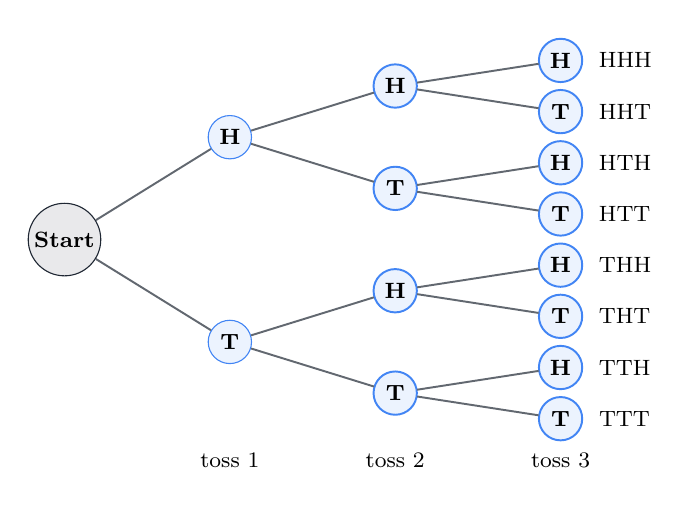
\begin{tikzpicture}[font=\sffamily\small,grow'=right,level distance=2.1cm,
  every node/.style={circle,draw=tmBlue,fill=tmBlue!10,inner sep=1.5pt,minimum size=0.55cm,font=\footnotesize\bfseries},
  level 1/.style={sibling distance=2.6cm},level 2/.style={sibling distance=1.3cm},level 3/.style={sibling distance=0.65cm},
  edge from parent/.style={draw=Ink!70,line width=0.7pt}]
\node[fill=Ink!10,draw=Ink] {Start}
  child {node {H}
    child {node {H} child {node {H}} child {node {T}}}
    child {node {T} child {node {H}} child {node {T}}}}
  child {node {T}
    child {node {H} child {node {H}} child {node {T}}}
    child {node {T} child {node {H}} child {node {T}}}};
\foreach \y/\t in {2.275/HHH,1.625/HHT,0.975/HTH,0.325/HTT,-0.325/THH,-0.975/THT,-1.625/TTH,-2.275/TTT}{
  \node[draw=none,fill=none,font=\footnotesize,anchor=west] at (6.7,\y) {\t};}
\node[draw=none,fill=none,font=\footnotesize] at (2.1,-2.8) {toss 1};
\node[draw=none,fill=none,font=\footnotesize] at (4.2,-2.8) {toss 2};
\node[draw=none,fill=none,font=\footnotesize] at (6.3,-2.8) {toss 3};
\end{tikzpicture}\end{center}
Example: the event ``exactly two heads'' consists of HHT, HTH, THH -- $3$ outcomes, so its probability is $\dfrac38$.

\begin{tipbox}
A problem like ``walk on a grid by tossing a coin'' (heads: move up, tails: move right) is really a problem about counting sequences of heads and tails: after $4$ tosses there are $2^4=16$ equally likely sequences, and the \emph{end point} depends only on the \emph{number of heads}, not on their order.
\end{tipbox}

% ----------------------------------------------------------------------
\shead{The multiplication rule and the addition rule}
\begin{knowbox}
\textbf{Multiplication rule.} If a task consists of two successive stages, stage 1 can be done in $m$ ways, and \emph{for each} way of doing stage 1, stage 2 can be done in $n$ ways, then the whole task can be done in $m\times n$ ways. (With three or four stages: keep multiplying.)

\medskip
\textbf{Addition rule (splitting into cases).} If the ways are split into cases that \emph{do not overlap}: case 1 has $a$ ways, case 2 has $b$ ways, \ldots, then the total number of ways is $a+b+\dots$

\medskip
\textbf{Common situations with digits.}
\begin{itemize}[leftmargin=1.2em,itemsep=1pt,topsep=2pt]
\item Three-digit numbers made from $3$ given non-zero digits, \emph{no repetition}: $3\times2\times1=6$ numbers.
\item Three-digit numbers made from $3$ given non-zero digits, \emph{repetition allowed}: $3\times3\times3=27$ numbers.
\item The first (leading) digit \textbf{cannot be $0$}: $9$ choices ($1$ to $9$); the other places have $10$ choices ($0$ to $9$).
\item A three-digit \textbf{palindrome} (reads the same forwards and backwards) has the form $\overline{aba}$: $9$ ways to choose $a$, $10$ ways to choose $b$, and the last digit is ``forced'' to equal $a$ (only $1$ way). There are $9\times10=90$ such numbers.
\end{itemize}
\end{knowbox}

\countboxes{hundreds/9/from 1 to 9/tmBlue,tens/10/from 0 to 9/tmOrange,ones/1/same as hundreds/tmGreen}{90}
\vspace{-6pt}
\begin{center}\footnotesize Number of three-digit palindromes: $9\times 10\times 1=90$.\end{center}

\begin{proofbox}
Why is the multiplication rule true? Draw a table with $m$ rows (the ways of doing stage 1) and $n$ columns (the ways of doing stage 2). Each cell of the table is \emph{exactly one} way of doing the whole task, and each way of doing the whole task is in \emph{exactly one} cell. The table has $m$ rows of $n$ cells, so $m\times n$ cells. A tree diagram gives the same result: $m$ big branches, each splitting into $n$ small branches.
\end{proofbox}

\begin{knowbox}
\textbf{Choosing two objects (order does not matter).} Choosing $2$ of $n$ students for classroom duty: if we care about order (first person, second person) there are $n\times(n-1)$ ways; but each pair is counted \emph{twice} (An--Bình and Bình--An), so the number of pairs is
\[
\frac{n\times(n-1)}{2}.
\]
Example: there are $\dfrac{10\times9}{2}=45$ pairs of different numbers taken from $10$ numbers.
\end{knowbox}

\begin{warnbox}
\textbf{Double counting.} When the question asks ``how many \emph{pairs}'', ``how many \emph{groups}'' (who comes first does not matter) and you use the multiplication rule with order, each group is counted several times -- you must divide. On the other hand, when the question is about \emph{numbers} (the order of the digits matters) or \emph{seating in a row}, order matters and you do \emph{not} divide.
\end{warnbox}

\begin{tipbox}
When splitting into cases, ask: ``Do the cases \emph{cover} every possibility? Do they \emph{overlap}?'' For example, for the sum $m+n$ to be even, $m$ and $n$ must be \emph{both odd} or \emph{both even} -- these two cases are separate and together they cover every possibility.
\end{tipbox}

% ----------------------------------------------------------------------
\shead{Reasoning by elimination: seating and colouring}
\begin{knowbox}
Some problems do not ask ``how many'' but ``\emph{who can}, \emph{who cannot}'', ``\emph{what is the least number needed}''. Then we use \textbf{reasoning}:
\begin{itemize}[leftmargin=1.2em,itemsep=1pt,topsep=2pt]
\item \textbf{Draw a diagram} of the positions (seats, cells, faces\ldots) and try filling it in.
\item Two people who \textbf{must sit together} can be treated as \textbf{one block} taking two neighbouring seats.
\item To show ``\emph{X can} sit in the middle seat'': just \textbf{give one arrangement} that satisfies all the conditions.
\item To show ``\emph{X cannot} sit in the middle seat'': \textbf{suppose} X sits in the middle seat and show that \emph{every} remaining arrangement breaks a condition (leading to a contradiction). This is called \textbf{proof by contradiction}.
\item A ``what is the \emph{least} number'' problem has \textbf{two parts}: (1) show a way that works with that number; (2) explain why fewer is impossible.
\end{itemize}
\end{knowbox}

\begin{figC}
\foreach \i in {1,...,5}{\draw[tmBlue,line width=1pt,fill=tmBlue!8,rounded corners=3pt] (\i*1.3-0.5,0) rectangle (\i*1.3+0.5,0.7);
  \node[font=\footnotesize] at (\i*1.3,-0.3){seat \i};}
\draw[tmOrange,line width=1.4pt,rounded corners=5pt] (3*1.3-0.62,-0.12) rectangle (3*1.3+0.62,0.82);
\node[font=\footnotesize\bfseries,text=tmOrange!80!black] at (3*1.3,1.1){middle seat};
\draw[decorate,decoration={brace,amplitude=5pt,mirror},Ink] (1*1.3-0.5,-0.55)--(2*1.3+0.5,-0.55) node[midway,below=5pt,font=\footnotesize]{two seats on the left};
\draw[decorate,decoration={brace,amplitude=5pt,mirror},Ink] (4*1.3-0.5,-0.55)--(5*1.3+0.5,-0.55) node[midway,below=5pt,font=\footnotesize]{two seats on the right};
\end{figC}
Key observation: once someone sits in the middle seat, the other four seats split into \emph{two pairs of neighbouring seats} (seats 1--2 and seats 4--5). The two seats on either side of the middle seat (seat 2 and seat 4) are \emph{not} next to each other.

\begin{knowbox}
\textbf{Colouring so that neighbouring parts have different colours.} Two faces of a cube are ``neighbours'' if they share an edge. Each face is a neighbour of $4$ faces and is \emph{not} a neighbour of exactly $1$ face -- the \textbf{opposite} face. A cube has $3$ pairs of opposite faces (top--bottom, front--back, left--right).
\begin{itemize}[leftmargin=1.2em,itemsep=1pt,topsep=2pt]
\item \emph{$3$ colours are enough:} paint each pair of opposite faces one colour; two faces of the same colour are opposite, so they are not neighbours.
\item \emph{Fewer than $3$ colours is impossible:} the three faces meeting at a corner are neighbours of each other in pairs, so they need three different colours.
\end{itemize}
\end{knowbox}

\begin{tipbox}
For a multiple-choice question ``Who \emph{cannot}\ldots?'', you can work backwards: for each option, try to find \emph{one} valid arrangement. Every option for which you find an arrangement is eliminated; the remaining option is the answer -- but remember to explain why it really cannot be arranged.
\end{tipbox}

% ----------------------------------------------------------------------
\shead{Counting shapes in a figure}
\begin{knowbox}
\textbf{Principle.} Counting shapes is a listing problem. To miss nothing and count nothing twice, \textbf{split into types} (by size, by position) and then \textbf{add up}.

\medskip
\textbf{The ``choose two lines'' trick.} A rectangle in a grid is completely determined by \emph{two horizontal lines} (top and bottom sides) and \emph{two vertical lines} (left and right sides). Therefore:
\begin{itemize}[leftmargin=1.2em,itemsep=1pt,topsep=2pt]
\item A strip of $1$ row and $n$ squares has $n+1$ vertical lines; the number of rectangles is the number of ways to choose $2$ vertical lines:
$\dfrac{(n+1)\times n}{2}$. Example: a strip of $4$ squares has $\dfrac{5\times4}{2}=10$ rectangles.
\item A grid with $a$ horizontal lines and $b$ vertical lines (all running the full length) has
$\dfrac{a(a-1)}{2}\times\dfrac{b(b-1)}{2}$ rectangles (multiplication rule!).
\item The same counting works for \emph{parallelograms} in a grid whose slanted lines are parallel to each other.
\end{itemize}
\end{knowbox}

\begin{figC}
\begin{scope}
\foreach \i in {0,...,4}{\draw[Ink,line width=1pt] (\i,0)--(\i,1); \node[font=\footnotesize,text=tmBlue] at (\i,-0.3){\pgfmathtruncatemacro\k{\i+1}\k};}
\draw[Ink,line width=1pt] (0,0)--(4,0) (0,1)--(4,1);
\fill[tmOrange,opacity=0.3] (1,0) rectangle (3,1);
\node[font=\footnotesize,align=center] at (2,-0.95){Choose vertical lines $2$ and $4$\\ $\Rightarrow$ the orange rectangle};
\end{scope}
\begin{scope}[xshift=6cm]
\foreach \x in {0,1,2,3}{\draw[Ink,line width=1pt] (\x,0)--(\x,2);}
\foreach \y in {0,1,2}{\draw[Ink,line width=1pt] (0,\y)--(3,\y);}
\fill[tmGreen,opacity=0.3] (1,0) rectangle (3,2);
\node[font=\footnotesize,align=center] at (1.5,-0.7){$3$ horizontal, $4$ vertical lines:\\ $3\times 6=18$ rectangles};
\end{scope}
\end{figC}

\begin{proofbox}
Why does a strip of $n$ squares have $\dfrac{(n+1)\times n}{2}$ rectangles? Choose the left side: $n+1$ ways; choose the right side (different from the left side): $n$ ways -- that gives $(n+1)\times n$ \emph{ordered} choices. But choosing ``line 2 then line 4'' or ``line 4 then line 2'' gives the same rectangle, so each rectangle is counted $2$ times; divide by $2$. Counting by size gives the same result: a strip of $4$ squares has $4$ rectangles of width $1$, $3$ of width $2$, $2$ of width $3$ and $1$ of width $4$, in total $4+3+2+1=10$.
\end{proofbox}

\begin{warnbox}
When the shapes \textbf{partly overlap} (not a grid with full-length lines), the ``choose two lines'' trick \emph{does not work}, because many segments do not run all the way across. Check each shape: \textbf{are all four sides really drawn?} Do not count ``imaginary rectangles'' that are missing a side.
\end{warnbox}

\begin{knowbox}
\textbf{Counting in a tiling.} A tiling made of regular octagons and small squares: if there are $m$ rows with $n$ octagons in each row, there are $m\times n$ octagons. Each small square sits where \emph{four octagons meet}; between $n$ columns there are $n-1$ gaps and between $m$ rows there are $m-1$ gaps, so there are $(m-1)\times(n-1)$ squares.
\end{knowbox}
\begin{figC}
\foreach \i in {0,1,2}{\foreach \j in {0,1}{\cpOct{\i}{\j}}}
\foreach \i in {0.5,1.5}{\cpDia{\i}{0.5}}
\node[font=\footnotesize,align=left,anchor=west] at (3,0.5){$2$ rows, $3$ columns: $2\times3=6$ octagons,\\ $(2-1)\times(3-1)=2$ squares.};
\end{figC}

% ----------------------------------------------------------------------
\shead{Counting with patterns: evenly spaced sequences, constant rates}
\begin{knowbox}
\textbf{Counting the whole numbers from $a$ to $b$} (including $a$ and $b$): there are $b-a+1$ numbers. For example from $1$ to $11$ there are $11$ numbers, of which $6$ are odd ($1,3,5,7,9,11$) and $5$ are even.

\medskip
\textbf{Evenly spaced sequence} (each number is a fixed amount $d$ more than the one before):
\[
\text{number of terms}=\frac{\text{last}-\text{first}}{d}+1,\qquad
\text{sum}=\frac{(\text{first}+\text{last})\times\text{number of terms}}{2}.
\]

\textbf{Quantities that change at a constant rate} (moving steadily, flowing steadily, counting steadily\ldots):
$\text{amount}=\text{rate}\times\text{time}$. For example, if $3$ sheep pass each minute, then in $14$ minutes $3\times14=42$ sheep pass.

\medskip
\textbf{Figures made of sticks.} Count the \emph{horizontal sticks} and the \emph{vertical sticks} separately and then add -- usually easier than counting square by square.

\medskip
\textbf{Events that repeat in cycles.} If one thing repeats every $a$ minutes and another every $b$ minutes, and they start together, they coincide again every $\text{LCM}(a,b)$ minutes.
\end{knowbox}

\begin{proofbox}
\textbf{Gauss's way of adding.} Compute $S=1+2+3+\dots+10$. Write the sum twice, once forwards and once backwards:
\[
\begin{array}{rcccccc}
S&=&1&+\;2&+\;3&+\dots+&10\\
S&=&10&+\;9&+\;8&+\dots+&1\\ \hline
2S&=&11&+\;11&+\;11&+\dots+&11
\end{array}
\]
There are $10$ columns, each with sum $11$, so $2S=10\times11=110$ and $S=55$. In general: sum $=\dfrac{(\text{first}+\text{last})\times\text{number of terms}}{2}$.
\end{proofbox}

\begin{warnbox}
\textbf{The ``off by one'' error.} From $3$ to $10$ there are $10-3+1=8$ numbers, \emph{not} $7$. A fence $10$ m long with a post every $1$ m (including both ends) needs $11$ posts, not $10$. Test a formula on a small example to check it.
\end{warnbox}

\begin{parentbox}
For ``toothpick'' problems, let your child actually build the small figures ($1$ square, $2$ squares, $3$ squares\ldots) with toothpicks, write the number of toothpicks in a table, and then ask: ``each time we add one square, how many toothpicks do we add?''. A child who finds the pattern alone remembers it much longer than a memorised formula.
\end{parentbox}

\begin{knowbox}
\textbf{Summary: read the clues, choose the tool.}\par\smallskip
\begin{tabularx}{\linewidth}{@{}>{\raggedright\arraybackslash}X>{\raggedright\arraybackslash}X@{}}
\textbf{Clue in the problem} & \textbf{Tool to use}\\ \hline
``choose one at random'', ``what is the probability'' & count all outcomes and favourable outcomes, then divide\\
probability given, quantity asked & favourable $=P\times$ total\\
something was taken out/eaten before the next draw & recount numerator and denominator\\
``at least one'', ``not'' & complement: $1-P$\\
two dice, two independent choices & two-way table\\
tossing a coin several times, several stages in a row & tree diagram\\
``how many numbers can be made'', ``how many ways'' & multiplication rule (choose restricted positions first)\\
``how many pairs'' (order does not matter) & multiplication rule, then divide by $2$\\
conditions of the form ``either\ldots or\ldots'' & split into cases, add\\
``who can / cannot'' & try one arrangement / proof by contradiction\\
``how many shapes\ldots'' & split by size, or choose two lines\\
rows of seats, toothpicks, constant rates & find the pattern, evenly spaced sequences\\
\end{tabularx}
\end{knowbox}

% ======================================================================
% EXAMPLES
% ======================================================================
\begin{exbox}{Example 1}
A box contains $3$ red marbles, $5$ blue marbles and $4$ yellow marbles, all of the same size. One marble is drawn at random.
\begin{enumerate}[label=\alph*),leftmargin=1.5em,itemsep=0pt,topsep=2pt]
\item Find the probability of drawing a blue marble.
\item Find the probability of drawing a marble that is \emph{not} red.
\item Find the probability of drawing a purple marble.
\end{enumerate}
\guide
\step{1}{Count all possible outcomes}
Each marble is one outcome, and since the marbles have the same size the outcomes are equally likely. Total number of marbles: $3+5+4=12$. So there are $12$ possible outcomes.
\step{2}{Part a}
There are $5$ blue marbles, i.e.\ $5$ favourable outcomes.
$P(\text{blue})=\dfrac{5}{12}$.
\step{3}{Part b -- use the complement}
$P(\text{red})=\dfrac{3}{12}=\dfrac14$, so $P(\text{not red})=1-\dfrac14=\dfrac34$.

\emph{Another way (direct counting):} the marbles that are not red are $5$ blue and $4$ yellow, i.e.\ $9$ marbles; $P=\dfrac{9}{12}=\dfrac34$. Both ways give the same result.
\step{4}{Part c}
There are no purple marbles in the box: $0$ favourable outcomes. $P(\text{purple})=\dfrac{0}{12}=0$ -- an impossible event.
\ans{a) $\frac{5}{12}$;\quad b) $\frac34$;\quad c) $0$.}
\end{exbox}

\begin{exbox}{Example 2}
A bag contains $30$ sweets, some strawberry and some orange. If one sweet is drawn at random, the probability that it is strawberry is $\dfrac25$.
\begin{enumerate}[label=\alph*),leftmargin=1.5em,itemsep=0pt,topsep=2pt]
\item How many strawberry sweets and how many orange sweets are in the bag?
\item An takes out $2$ strawberry sweets and eats them. Then Bình draws one sweet at random from the bag. Find the probability that Bình gets a strawberry sweet.
\end{enumerate}
\guide
\step{1}{Find the number of strawberry sweets}
\begin{recallbox}Number of favourable outcomes $=$ probability $\times$ number of all outcomes.\end{recallbox}
Strawberry sweets: $30\times\dfrac25=\dfrac{30\times 2}{5}=\dfrac{60}{5}=12$. Orange sweets: $30-12=18$.

\emph{Check:} $\dfrac{12}{30}=\dfrac{2}{5}$ \checkmark.
\step{2}{Recount after An eats $2$ sweets}
\begin{center}
\begin{tabular}{|l|c|c|c|}\hline
 & strawberry & orange & total \\ \hline
At the start & $12$ & $18$ & $30$\\ \hline
After An eats $2$ strawberry & $12-2=10$ & $18$ & $30-2=28$\\ \hline
\end{tabular}
\end{center}
\step{3}{Compute the probability for Bình}
$P(\text{strawberry})=\dfrac{10}{28}=\dfrac{5}{14}$.
\begin{warnbox}Do not answer $\dfrac{10}{30}$: An has eaten $2$ sweets, so the total number of sweets (the denominator) has gone down too.\end{warnbox}
\ans{a) $12$ strawberry, $18$ orange;\quad b) $\frac{5}{14}$.}
\end{exbox}

\begin{exbox}{Example 3}
A red die and a blue die (both fair) are rolled together. Find the probability of each event:
\begin{enumerate}[label=\alph*),leftmargin=1.5em,itemsep=0pt,topsep=2pt]
\item The sum of the two numbers is $8$.
\item Both dice show the same number.
\item The sum of the two numbers is greater than or equal to $10$.
\end{enumerate}
\guide
\step{1}{Make a table of all outcomes}
Rows are the numbers on the red die, columns the numbers on the blue die, and each cell shows the sum. The table has $6\times6=36$ cells, corresponding to $36$ equally likely outcomes.
\begin{figC}
\foreach \c in {1,...,6}{\node[draw=tmBlue,fill=tmBlue!15,minimum size=0.6cm,font=\bfseries] at (\c*0.6,0.4) {\c};}
\foreach \r in {1,...,6}{\node[draw=AnsRed,fill=AnsRed!12,minimum size=0.6cm,font=\bfseries] at (0,0.4-\r*0.6) {\r};
  \foreach \c in {1,...,6}{\pgfmathtruncatemacro\s{\r+\c}%
    \def\fc{white}%
    \ifnum\s=8 \def\fc{tmOrange!40}\fi
    \ifnum\s>9 \def\fc{tmGreen!30}\fi
    \node[draw=Line,fill=\fc,minimum size=0.6cm] at (\c*0.6,0.4-\r*0.6) {\s};
    \ifnum\r=\c \draw[tmPurple,line width=1pt] (\c*0.6,0.4-\r*0.6) circle (0.24);\fi}}
\node[font=\footnotesize,align=left,anchor=west] at (4.4,-1.7) {\colorbox{tmOrange!40}{\strut\ \ } sum equals $8$ ($5$ cells)\\[2pt]
  {\color{tmPurple}$\bigcirc$} both numbers equal ($6$ cells)\\[2pt] \colorbox{tmGreen!30}{\strut\ \ } sum $\ge 10$ ($6$ cells)};
\end{figC}
\step{2}{Part a}
The cells with sum $8$: $(2,6),(3,5),(4,4),(5,3),(6,2)$ -- $5$ outcomes (the first number is the red die). $P=\dfrac{5}{36}$.
\step{3}{Part b}
Equal numbers lie on the diagonal: $(1,1),(2,2),\dots,(6,6)$ -- $6$ outcomes. $P=\dfrac{6}{36}=\dfrac16$.
\step{4}{Part c}
Sum $10$: $(4,6),(5,5),(6,4)$; sum $11$: $(5,6),(6,5)$; sum $12$: $(6,6)$. Altogether $3+2+1=6$ outcomes. $P=\dfrac{6}{36}=\dfrac16$.
\begin{tipbox}The $6\times6$ table also shows \emph{symmetry}: the number of cells above the diagonal (red smaller than blue) equals the number of cells below the diagonal (red greater than blue).\end{tipbox}
\ans{a) $\frac{5}{36}$;\quad b) $\frac16$;\quad c) $\frac16$.}
\end{exbox}

\begin{exbox}{Example 4}
A fair coin is tossed three times in a row. Find the probability of getting:
a) exactly two heads;\quad b) at least one head.
\guide
\step{1}{Draw a tree diagram and list}
Each toss has $2$ outcomes (H or T). By the tree diagram in section 3, there are $2\times2\times2=8$ equally likely outcomes:
\[
\text{HHH},\ \text{HHT},\ \text{HTH},\ \text{HTT},\ \text{THH},\ \text{THT},\ \text{TTH},\ \text{TTT}.
\]
\step{2}{Part a}
The outcomes with exactly two H's: HHT, HTH, THH -- $3$ outcomes. $P=\dfrac38$.
\step{3}{Part b -- complement}
The complement of ``at least one head'' is ``no heads at all'', which is only TTT ($1$ outcome). So
$P(\text{at least one H})=1-\dfrac18=\dfrac78$.
\begin{tipbox}When you see the words ``\emph{at least one}'', think immediately of the complement ``\emph{none at all}'' -- it usually has very few outcomes and is easy to count.\end{tipbox}
\ans{a) $\frac38$;\quad b) $\frac78$.}
\end{exbox}

\begin{exbox}{Example 5}
Using the digits $1,2,3,4$, how many three-digit numbers can be made if:
a) digits may be repeated;\quad b) the digits must be different;\quad c) the digits are different and the number is even?\\
d) One of the numbers from part b) is chosen at random. Find the probability that it is even.
\guide
\step{1}{Part a -- repetition allowed}
Hundreds: $4$ ways; tens: still $4$ ways; ones: $4$ ways. By the multiplication rule: $4\times4\times4=64$ numbers.
\step{2}{Part b -- no repetition}
\countboxes{hundreds/4/any/tmBlue,tens/3/not the hundreds digit/tmOrange,ones/2/not the two above/tmGreen}{24}
Hundreds: $4$ ways. The tens digit must differ from the digit already used: $3$ ways. The ones digit must differ from both digits used: $2$ ways. There are $4\times3\times2=24$ numbers.
\step{3}{Part c -- even, no repetition: choose the ones digit FIRST}
An even number ends in $2$ or $4$: $2$ ways. Then the hundreds digit is one of the $3$ remaining digits: $3$ ways; the tens digit: $2$ ways. There are $2\times3\times2=12$ numbers.
\begin{tipbox}A position with a \emph{condition} (must be even, must not be $0$\ldots) should be \textbf{chosen first}. If you choose the hundreds digit first, the number of choices for the ones digit is sometimes $1$ and sometimes $2$ (depending on whether the hundreds digit used an even or an odd digit) -- very easy to get wrong.\end{tipbox}
\step{4}{Part d}
$P(\text{even})=\dfrac{12}{24}=\dfrac12$.
\verify{List the numbers starting with $1$: $123,124,132,134,142,143$ -- exactly $6=3\times2$ numbers, of which $124,132,134,142$ are even ($4$ numbers). The four possible first digits behave alike, so there are $4\times6=24$ numbers, \ldots\ matching part b.}
\ans{a) $64$;\quad b) $24$;\quad c) $12$;\quad d) $\frac12$.}
\end{exbox}

\begin{exbox}{Example 6}
Four friends An, Bình, Chi and Dũng sit on four chairs in a row, numbered $1,2,3,4$ from left to right. We know that: Dũng sits on chair $1$; Bình and Chi sit next to each other; An does not sit next to Bình; An does not sit on chair $4$. Who sits on chair $4$?
\guide
\step{1}{Place Dũng}
Dũng is on chair $1$, leaving chairs $2,3,4$ for An, Bình and Chi.
\step{2}{Consider An's position}
An does not sit on chair $4$, so An sits on chair $2$ or chair $3$.
\begin{itemize}[leftmargin=1.2em,itemsep=1pt,topsep=1pt]
\item \emph{If An sits on chair $3$:} Bình and Chi take chairs $2$ and $4$ -- these chairs are not next to each other, which breaks the condition ``Bình and Chi sit next to each other''. Rejected.
\item \emph{If An sits on chair $2$:} Bình and Chi take chairs $3$ and $4$ (next to each other, good). An must not be next to Bình, and chair $3$ is next to chair $2$, so Bình is not on chair $3$. So Bình is on chair $4$ and Chi on chair $3$.
\end{itemize}
\begin{figC}
\foreach \i/\n/\c in {1/Dũng/tmPurple,2/An/tmOrange,3/Chi/tmGreen,4/Bình/tmBlue}{
  \draw[\c,line width=1pt,fill=\c!12,rounded corners=3pt] (\i*1.6-0.65,0) rectangle (\i*1.6+0.65,0.7);
  \node[font=\bfseries] at (\i*1.6,0.35){\n};\node[font=\footnotesize] at (\i*1.6,-0.3){chair \i};}
\end{figC}
\verify{Dũng on chair $1$ \checkmark; Bình (chair $4$) next to Chi (chair $3$) \checkmark; An (chair $2$) is next to Dũng and Chi, not next to Bình \checkmark; An is not on chair $4$ \checkmark.}
\ans{Bình sits on chair $4$.}
\end{exbox}

\begin{exbox}{Example 7}
a) The figure on the left is a strip of $4$ squares. How many rectangles (including squares) are there altogether?\\
b) The figure on the right is a $2\times2$ grid of squares. How many rectangles are there? How many of them are squares?
\begin{figC}
\foreach \i in {0,...,4}{\draw[Ink,line width=1pt] (\i*0.8,0)--(\i*0.8,0.8);}
\draw[Ink,line width=1pt] (0,0)--(3.2,0) (0,0.8)--(3.2,0.8);
\begin{scope}[xshift=5.5cm]
\foreach \i in {0,1,2}{\draw[Ink,line width=1pt] (\i*0.8,0)--(\i*0.8,1.6) (0,\i*0.8)--(1.6,\i*0.8);}
\end{scope}
\end{figC}
\guide
\step{1}{Part a -- count by width}
Measure the width in squares:
\begin{center}
\begin{tabular}{|c|c|c|c|c|}\hline
Width & $1$ square & $2$ squares & $3$ squares & $4$ squares\\ \hline
Number of shapes & $4$ & $3$ & $2$ & $1$\\ \hline
\end{tabular}
\end{center}
Total: $4+3+2+1=10$ rectangles. \emph{Check with the ``choose two vertical lines'' trick:} there are $5$ vertical lines, and the number of ways to choose $2$ of them is $\dfrac{5\times4}{2}=10$ \checkmark.
\step{2}{Part b -- choose two horizontal and two vertical lines}
The grid has $3$ horizontal and $3$ vertical lines. Choose $2$ horizontal lines: $\dfrac{3\times2}{2}=3$ ways; choose $2$ vertical lines: $3$ ways. By the multiplication rule there are $3\times3=9$ rectangles.
\step{3}{Count the squares separately}
$1\times1$ squares: $4$; $2\times2$ squares: $1$ (the whole grid). There are $4+1=5$ squares.
\verify{Counting by size: $1\times1$: $4$; $1\times2$ (lying flat): $2$; $2\times1$ (standing): $2$; $2\times2$: $1$. Total $4+2+2+1=9$ \checkmark.}
\ans{a) $10$ rectangles;\quad b) $9$ rectangles, of which $5$ are squares.}
\end{exbox}

\begin{exbox}{Example 8}
Toothpicks are used to make a row of joined squares as shown below.
\begin{figC}
\foreach \n/\x in {1/0,2/2,3/5}{
  \foreach \i in {0,...,\n}{\draw[tmOrange!80!black,line width=1.6pt,line cap=round] (\x+\i*0.7,0.05)--(\x+\i*0.7,0.65);}
  \foreach \i in {1,...,\n}{\draw[tmOrange!80!black,line width=1.6pt,line cap=round] (\x+\i*0.7-0.65,0)--(\x+\i*0.7-0.05,0) (\x+\i*0.7-0.65,0.7)--(\x+\i*0.7-0.05,0.7);}
  \node[font=\footnotesize] at (\x+\n*0.35,-0.35){\n\ sq.};}
\end{figC}
a) How many toothpicks are needed for a row of $20$ squares?\\
b) Lan builds, one after another and separately, a row of $1$ square, a row of $2$ squares, \ldots, a row of $10$ squares. How many toothpicks does Lan use altogether?
\guide
\step{1}{Find the pattern}
\begin{center}
\begin{tabular}{|c|c|c|c|c|}\hline
Squares & $1$ & $2$ & $3$ & $n$\\ \hline
Toothpicks & $4$ & $7$ & $10$ & $3n+1$\\ \hline
\end{tabular}
\end{center}
Explanation: count each kind of toothpick separately. Horizontal toothpicks: each square has $1$ on top and $1$ at the bottom, that is $2n$ toothpicks. Vertical toothpicks: $n$ squares have $n+1$ vertical toothpicks (just as $n$ gaps need $n+1$ posts). Total $2n+(n+1)=3n+1$.
\step{2}{Part a}
$n=20$: $3\times20+1=61$ toothpicks.
\step{3}{Part b -- sum of an evenly spaced sequence}
The numbers of toothpicks are $4,7,10,\dots,31$ (a row of $10$ squares needs $3\times10+1=31$ toothpicks). This is an evenly spaced sequence with step $3$ and $10$ terms.
\begin{recallbox}Sum of an evenly spaced sequence $=\dfrac{(\text{first}+\text{last})\times\text{number of terms}}{2}$.\end{recallbox}
Sum: $\dfrac{(4+31)\times10}{2}=\dfrac{350}{2}=175$ toothpicks.
\verify{$4+7+10+13+16+19+22+25+28+31$: pair first with last, $4+31=7+28=10+25=13+22=16+19=35$, giving $5$ pairs, $5\times35=175$ \checkmark.}
\ans{a) $61$ toothpicks;\quad b) $175$ toothpicks.}
\end{exbox}

% ======================================================================
\clearpage
\dividerbar{Core practice}

% ---------------------------------------------------------------- Problem 1
\begin{probbox}{1}{\relax}
\begin{minipage}[t]{0.66\linewidth}\vspace{0pt}
The spinner shown is divided into $6$ sectors of equal size, each marked with a letter. The spinner is spun once. What is the probability that the arrow lands on a sector marked with the letter $P$?
\choices{$\dfrac{3}{6}$}{$\dfrac{4}{6}$}{$\dfrac{5}{6}$}{$\dfrac{2}{6}$}{$\dfrac{1}{6}$}
\end{minipage}\hfill
\begin{minipage}[t]{0.3\linewidth}\vspace{0pt}
\centering\begin{tikzpicture}[scale=0.95]\cpSpinSix{P}{R}{P}{Q}{R}{Q}\end{tikzpicture}
\end{minipage}
\end{probbox}
\probsol{
\textbf{Understanding the problem.} The spinner has $6$ \emph{equal} sectors, so when it is spun the arrow is equally likely to stop in each sector. We need the probability that the arrow points to a sector marked $P$.
\begin{recallbox}When the outcomes are equally likely: $P(\text{event})=\dfrac{\text{number of favourable outcomes}}{\text{number of all outcomes}}$.\end{recallbox}
\step{1}{Count all possible outcomes}
The arrow can stop in any one of the $6$ sectors, so there are $6$ possible outcomes.
\step{2}{Count the favourable outcomes}
Reading the letters clockwise, starting from the top-left sector: $P,\ R,\ P,\ Q,\ R,\ Q$. Exactly $2$ sectors are marked $P$ (the top-left one and the right one).
\step{3}{Compute the probability}
$P(\text{letter }P)=\dfrac{2}{6}$ $\left(=\dfrac13\right)$.
\begin{warnbox}There are $3$ different letters ($P$, $Q$, $R$), but the probability is \emph{not} computed as ``$1$ letter out of $3$ letters''. Here $\dfrac13=\dfrac26$ only by coincidence, because each letter appears exactly $2$ times; if the letters took up different numbers of sectors, that way of thinking would be wrong. Always count \emph{sectors}, not \emph{kinds of letters}.\end{warnbox}
\verify{Each of the letters $P$, $Q$, $R$ takes $2$ sectors: $\dfrac26+\dfrac26+\dfrac26=1$ -- the probabilities of all possibilities add up to $1$, as they should.}
The value $\dfrac26$ matches option \textbf{(D)}. (Option (A) $\dfrac36$ comes from miscounting $3$ sectors; (E) $\dfrac16$ is the probability of \emph{one} particular sector.)
\ans{(D) $\dfrac{2}{6}$}
}

% ---------------------------------------------------------------- Problem 2
\begin{probbox}{2}{\relax}
Using the three digits $4$, $7$ and $9$, each digit used \emph{at most once}, how many three-digit whole numbers with different digits can be made?
\choices{$6$}{$3$}{$5$}{$12$}{$9$}
\end{probbox}
\probsol{
\textbf{Understanding the problem.} A three-digit number using exactly the digits $4,7,9$, with no digit repeated. So each number is an \emph{arrangement} of these three digits in the three places: hundreds, tens, ones.
\step{1}{Method 1 -- systematic listing}
Order by the hundreds digit (from smallest to largest):
\begin{itemize}[leftmargin=1.2em,itemsep=0pt,topsep=1pt]
\item Hundreds digit $4$: the other two digits $7,9$ give $479$ and $497$.
\item Hundreds digit $7$: $749$ and $794$.
\item Hundreds digit $9$: $947$ and $974$.
\end{itemize}
There are $2+2+2=6$ numbers.
\step{2}{Method 2 -- multiplication rule}
\begin{recallbox}Multiplication rule: if a task has several successive stages, each with a number of ways (not depending on the choices made before), then the number of ways to do the whole task is the \emph{product} of those numbers.\end{recallbox}
\countboxes{hundreds/3/4 or 7 or 9/tmBlue,tens/2/2 digits left/tmOrange,ones/1/the last digit/tmGreen}{6}
Hundreds: $3$ choices. Tens: only $2$ unused digits remain, $2$ choices. Ones: exactly $1$ digit remains, $1$ choice. Number of numbers: $3\times2\times1=6$.
\begin{warnbox}If repeated digits were allowed there would be $3\times3\times3=27$ numbers (such as $444$, $477$\ldots). The problem forbids repetition, so after each stage the number of choices goes down by $1$.\end{warnbox}
\verify{The six numbers $479,497,749,794,947,974$ are all different and all use the three digits. Both methods give the same result.}
The answer $6$ is option \textbf{(A)}. (Option (B) $3$ is just the number of digits given.)
\ans{(A) $6$}
}

% ---------------------------------------------------------------- Problem 3
\begin{probbox}{3}{\relax}
An envelope contains $2$ sunflower seeds, $3$ mung bean seeds and $4$ pumpkin seeds. Chi takes one seed from the envelope at random. What is the probability that Chi takes a sunflower seed?
\choices{$\dfrac{2}{9}$}{$\dfrac{5}{9}$}{$\dfrac{9}{7}$}{$\dfrac{7}{9}$}{$\dfrac{1}{9}$}
\end{probbox}
\probsol{
\textbf{Understanding the problem.} The envelope has three kinds of seeds in different numbers. Chi takes \emph{one seed} at random: every seed has the same chance of being taken, so each \emph{seed} is one equally likely outcome.
\step{1}{Count all possible outcomes}
Total number of seeds: $2+3+4=9$, i.e.\ $9$ outcomes.
\step{2}{Count the favourable outcomes}
There are $2$ sunflower seeds, so $2$ favourable outcomes.
\step{3}{Compute the probability}
\begin{recallbox}$P=\dfrac{\text{number of favourable outcomes}}{\text{number of all outcomes}}$.\end{recallbox}
$P(\text{sunflower})=\dfrac{2}{9}$.
\begin{warnbox}There are $3$ \emph{kinds} of seeds but the answer is not $\dfrac13$, because the pumpkin seeds are more numerous and so more likely to be taken. Remember too that a probability is never greater than $1$, so option (C) $\dfrac97$ is certainly wrong.\end{warnbox}
\verify{$P(\text{sunflower})+P(\text{mung bean})+P(\text{pumpkin})=\dfrac29+\dfrac39+\dfrac49=\dfrac99=1$.}
The result $\dfrac29$ is option \textbf{(A)}. (Option (D) $\dfrac79$ is the probability of \emph{not} taking a sunflower seed.)
\ans{(A) $\dfrac{2}{9}$}
}

% ---------------------------------------------------------------- Problem 4
\begin{probbox}{4}{\relax}
A cinema has $11$ rows of seats, numbered from $1$ to $11$. Each odd-numbered row has $15$ seats and each even-numbered row has $16$ seats. How many seats are there in the cinema altogether?
\choices{$176$}{$186$}{$165$}{$170$}{$171$}
\end{probbox}
\probsol{
\textbf{Understanding the problem.} The number of seats in a row depends on whether the row number is odd or even. So we need to know how many of the numbers from $1$ to $11$ are odd and how many are even.
\step{1}{Count the odd rows and the even rows}
Odd rows: $1,3,5,7,9,11$ -- $6$ rows.\\
Even rows: $2,4,6,8,10$ -- $5$ rows.\\
Check: $6+5=11$ rows \checkmark.
\begin{figC}
\foreach \i in {1,...,11}{\pgfmathtruncatemacro\m{mod(\i,2)}%
  \ifnum\m=1 \def\cc{tmBlue}\else\def\cc{tmOrange}\fi
  \draw[\cc,line width=0.9pt,fill=\cc!15,rounded corners=2pt] (\i*0.75-0.33,0) rectangle (\i*0.75+0.33,0.55);
  \node[font=\footnotesize\bfseries] at (\i*0.75,0.275){\i};}
\node[font=\footnotesize,text=tmBlue!80!black,anchor=west] at (9,0.55){odd row: $15$ seats};
\node[font=\footnotesize,text=tmOrange!80!black,anchor=west] at (9,0.05){even row: $16$ seats};
\end{figC}
\begin{warnbox}Do not split the $11$ rows into ``$5.5$ odd rows and $5.5$ even rows''. The list starts \emph{and} ends with an odd number ($1$ and $11$), so there is exactly $1$ more odd number than even numbers.\end{warnbox}
\step{2}{Seats in the odd rows}
$6\times15=90$ seats.
\step{3}{Seats in the even rows}
$5\times16=80$ seats.
\step{4}{Add up}
Total number of seats: $90+80=170$.
\verify{\emph{Another way -- pairing:} pair row $1$ with row $2$, row $3$ with row $4$, \ldots, row $9$ with row $10$: that gives $5$ pairs, each with $15+16=31$ seats, i.e.\ $5\times31=155$ seats; row $11$ with $15$ seats is left over. Total $155+15=170$ \checkmark.}
The answer $170$ is option \textbf{(D)}. (Mixing up and taking $5$ odd rows and $6$ even rows gives $171$ -- option (E), a very common ``trap''.)
\ans{(D) $170$}
}

% ---------------------------------------------------------------- Problem 5
\begin{probbox}{5}{\relax}
At a class party, each student in turn draws a wrapped present at random from a bag. The presents are only books and calculators; there are $27$ presents in the bag altogether. Mai draws first. The probability that Mai draws a book is $\dfrac23$. How many books are in the bag?
\choices{$15$}{$9$}{$21$}{$7$}{$18$}
\end{probbox}
\probsol{
\textbf{Understanding the problem.} A ``backwards'' problem: we know the \emph{probability} and the \emph{total} number of presents, and need the \emph{number of favourable outcomes} (the number of books). Since Mai draws first, all $27$ presents are still in the bag.
\begin{recallbox}From $P=\dfrac{\text{number of favourable outcomes}}{\text{number of all outcomes}}$ we get: number of favourable outcomes $=P\times$ number of all outcomes.\end{recallbox}
\step{1}{Call the number of books an unknown}
Let the number of books be $s$. The probability of drawing a book is $\dfrac{s}{27}$. By the problem: $\dfrac{s}{27}=\dfrac23$.
\step{2}{Find $s$}
$s=27\times\dfrac23=\dfrac{27\times2}{3}=\dfrac{54}{3}=18$.

\emph{Thinking with a bar model:} $\dfrac23$ means splitting the $27$ presents into $3$ equal parts of $27\div3=9$ presents each; books take $2$ parts, i.e.\ $2\times 9=18$ books.
\begin{figC}
\blk{0}{3}{0}{0.6}{tmBlue}{9 books}\blk{3}{6}{0}{0.6}{tmBlue}{9 books}\blk{6}{9}{0}{0.6}{tmOrange}{9 calculators}
\brcup{0}{9}{0.5}{$27$ presents}
\brcdn{0}{6}{-0.5}{$\frac23$ are books: $18$ books}
\end{figC}
\verify{There are $18$ books and $27-18=9$ calculators. Probability of drawing a book: $\dfrac{18}{27}=\dfrac{18\div9}{27\div9}=\dfrac23$ \checkmark.}
\begin{warnbox}The $9$ in option (B) is the number of \emph{calculators}, not books -- read the question carefully before choosing.\end{warnbox}
The answer $18$ is option \textbf{(E)}.
\ans{(E) $18$}
}

% ---------------------------------------------------------------- Problem 6
\begin{probbox}{6}{\relax}
A crate of fruit contains $20$ apples, $10$ oranges and no other fruit. One fruit is taken from the crate at random. What is the probability that it is an orange?
\choices{$\dfrac{1}{10}$}{$\dfrac{1}{20}$}{$\dfrac{1}{30}$}{$\dfrac{1}{3}$}{$\dfrac{2}{3}$}
\end{probbox}
\probsol{
\textbf{Understanding the problem.} Every fruit in the crate has the same chance of being taken. A favourable outcome is taking one of the oranges.
\step{1}{Count all outcomes}
Total number of fruits: $20+10=30$.
\step{2}{Count the favourable outcomes}
There are $10$ oranges.
\step{3}{Compute and simplify}
\begin{recallbox}$P=\dfrac{\text{number of favourable outcomes}}{\text{number of all outcomes}}$; simplify a fraction by dividing the numerator and denominator by their GCD.\end{recallbox}
$P(\text{orange})=\dfrac{10}{30}=\dfrac{10\div10}{30\div10}=\dfrac13$.
\begin{warnbox}Two common mistakes: (1) using the number of apples ($20$) as the denominator instead of the \emph{total number of fruits} ($30$), giving $\dfrac{10}{20}$; (2) writing $\dfrac{1}{10}$ (option A) thinking ``there are $10$ oranges so each is $\dfrac1{10}$''. The denominator is always \emph{all} the outcomes.\end{warnbox}
\verify{$P(\text{apple})=\dfrac{20}{30}=\dfrac23$ and $\dfrac13+\dfrac23=1$ \checkmark. It also makes sense: there are twice as many apples as oranges, so an apple is twice as likely as an orange.}
The result $\dfrac13$ is option \textbf{(D)}. (Option (E) $\dfrac23$ is the probability of taking an apple.)
\ans{(D) $\dfrac13$}
}

% ---------------------------------------------------------------- Problem 7
\begin{probbox}{7}{\relax}
A bag contains $2$ red balls, $5$ yellow balls and $4$ blue balls, all the same size. Without looking, one ball is taken from the bag. The probability of taking a yellow ball is
\choices{$\dfrac{2}{11}$}{$\dfrac{5}{11}$}{$\dfrac{4}{11}$}{$\dfrac{6}{11}$}{$\dfrac{7}{11}$}
\end{probbox}
\probsol{
\textbf{Understanding the problem.} ``Without looking'' and ``the same size'' guarantee that every ball has the same chance of being taken.
\step{1}{Count all outcomes}
Total number of balls: $2+5+4=11$.
\step{2}{Count the favourable outcomes}
There are $5$ yellow balls.
\step{3}{Compute the probability}
\begin{recallbox}$P=\dfrac{\text{number of favourable outcomes}}{\text{number of all outcomes}}$.\end{recallbox}
$P(\text{yellow})=\dfrac{5}{11}$ (this fraction is already in lowest terms because $5$ and $11$ have no common factor other than $1$).
\begin{figC}
\foreach \i in {1,2}{\shade[ball color=AnsRed] (\i*0.6,0) circle (0.22);}
\foreach \i in {3,...,7}{\shade[ball color=tmOrange] (\i*0.6+0.3,0) circle (0.22);\draw[tmOrange!70!black,line width=0.8pt] (\i*0.6+0.3,0) circle (0.27);}
\foreach \i in {8,...,11}{\shade[ball color=tmBlue] (\i*0.6+0.6,0) circle (0.22);}
\node[font=\footnotesize] at (3.9,-0.55){$5$ of the $11$ balls are yellow};
\end{figC}
\verify{$\dfrac{2}{11}+\dfrac{5}{11}+\dfrac{4}{11}=\dfrac{11}{11}=1$ \checkmark.}
The distractors: (A) $\dfrac{2}{11}$ is the probability of red, (C) $\dfrac{4}{11}$ the probability of blue, (D) $\dfrac{6}{11}$ the probability of \emph{not} taking a yellow ball. The correct answer is \textbf{(B)}.
\ans{(B) $\dfrac{5}{11}$}
}

% ---------------------------------------------------------------- Problem 8
\begin{probbox}{8}{\relax}
You are doing a multiple-choice test. On one question you do not know the answer, so you choose an option at random. If the question has five options (A, B, C, D, E) and only one of them is correct, what is the probability that you guess correctly?
\choices{$\dfrac{1}{5}$}{$\dfrac{5}{5}$}{$\dfrac{4}{5}$}{$\dfrac{2}{5}$}{$\dfrac{3}{5}$}
\end{probbox}
\probsol{
\textbf{Understanding the problem.} ``Choose at random'' means the five options are equally likely to be chosen. The question has exactly \emph{one} correct option.
\step{1}{Count all outcomes}
There are $5$ options to choose from: A, B, C, D, E.
\step{2}{Count the favourable outcomes}
Only $1$ option is correct, so there is $1$ favourable outcome.
\step{3}{Compute the probability}
\begin{recallbox}$P=\dfrac{\text{number of favourable outcomes}}{\text{number of all outcomes}}$.\end{recallbox}
$P(\text{correct})=\dfrac15$.
\begin{tipbox}The probability of guessing \emph{wrong} is $1-\dfrac15=\dfrac45$ -- option (C). So when guessing you are $4$ times more likely to be wrong than right. And (B) $\dfrac55=1$ means ``certainly correct'' -- absurd for a guess.\end{tipbox}
\verify{If you did $100$ such questions and guessed every one, you would get about $100\times\dfrac15=20$ right on average -- matching the feeling ``$1$ right out of every $5$''.}
The answer is \textbf{(A)}.
\ans{(A) $\dfrac15$}
}

% ---------------------------------------------------------------- Problem 9
\begin{probbox}{9}{\relax}
A fair six-sided die has the numbers $1$ to $6$ on its faces. The die is rolled once. What is the probability that it shows a $5$?
\choices{$\dfrac{2}{6}$}{$\dfrac{1}{6}$}{$\dfrac{5}{6}$}{$\dfrac{3}{6}$}{$\dfrac{4}{6}$}
\end{probbox}
\probsol{
\textbf{Understanding the problem.} The die is \emph{fair}, so the six faces are equally likely. The event we care about: ``the face showing is $5$''.
\step{1}{List the possible outcomes}
$\{1,\,2,\,3,\,4,\,5,\,6\}$ -- $6$ equally likely outcomes.
\step{2}{Count the favourable outcomes}
Only one face shows $5$: $1$ favourable outcome.
\step{3}{Compute the probability}
\begin{recallbox}$P=\dfrac{\text{number of favourable outcomes}}{\text{number of all outcomes}}$.\end{recallbox}
$P(5)=\dfrac16$.
\begin{warnbox}Do not confuse ``the number $5$'' with ``the number of favourable outcomes''. Many students write $\dfrac56$ (option C) because they see a $5$ in the question. The $5$ is only the \emph{name} of the face; the number of faces with that name is only $1$. ($\dfrac56$ is the probability of rolling a number \emph{from $1$ to $5$}, i.e.\ anything but $6$.)\end{warnbox}
\verify{Each face has probability $\dfrac16$, and the six faces together give $\dfrac66=1$ \checkmark.}
The answer is \textbf{(B)}.
\ans{(B) $\dfrac16$}
}

% ---------------------------------------------------------------- Problem 10
\begin{probbox}{10}{\relax}
Five friends An, Hà, Chi, Minh and Tùng sit in a row of five seats. An does \emph{not} sit next to Hà, and Chi sits next to Minh. Who \emph{cannot} sit in the middle seat?
\choices{An}{Hà}{Chi}{Minh}{Tùng}
\end{probbox}
\probsol{
\textbf{Understanding the problem.} The five seats are in a row, numbered $1,2,3,4,5$ from left to right; the middle seat is seat $3$. Two conditions: (i) An and Hà do \emph{not} sit next to each other; (ii) Chi and Minh sit next to each other. We must find the friend who can \emph{never} sit in seat $3$.
\begin{recallbox}To show that a friend \emph{can} sit in the middle: just give \emph{one} arrangement satisfying every condition. To show that a friend \emph{cannot}: suppose they sit in the middle and show that every arrangement then breaks a condition (proof by contradiction).\end{recallbox}
\step{1}{An, Hà, Chi and Minh can each sit in the middle}
Here is one arrangement for each of them (seats $1\to5$):
\begin{center}
\begin{tabular}{|c|c|c|c|c|c|l|}\hline
In the middle & seat 1 & seat 2 & \textbf{seat 3} & seat 4 & seat 5 & check\\ \hline
An & Chi & Minh & \textbf{An} & Tùng & Hà & An (3), Hà (5) not neighbours\\ \hline
Hà & Chi & Minh & \textbf{Hà} & Tùng & An & Hà (3), An (5) not neighbours\\ \hline
Chi & An & Minh & \textbf{Chi} & Tùng & Hà & Chi (3) next to Minh (2)\\ \hline
Minh & An & Chi & \textbf{Minh} & Tùng & Hà & Minh (3) next to Chi (2)\\ \hline
\end{tabular}
\end{center}
In all four arrangements Chi and Minh are always neighbours, and An and Hà are always apart (An in seat $1$ or $3$, Hà in seat $5$, or the other way round). So options (A), (B), (C), (D) are eliminated.
\step{2}{Show that Tùng cannot sit in the middle}
Suppose Tùng sits in seat $3$. The other four seats split into two pairs of neighbouring seats: the left pair (seats $1$--$2$) and the right pair (seats $4$--$5$). Note that seats $2$ and $4$ are \emph{not} neighbours (Tùng is between them).
\begin{figC}
\foreach \i/\n/\c in {1/?/tmBlue,2/?/tmBlue,3/Tùng/tmOrange,4/?/tmGreen,5/?/tmGreen}{
  \draw[\c,line width=1pt,fill=\c!12,rounded corners=3pt] (\i*1.5-0.6,0) rectangle (\i*1.5+0.6,0.65);
  \node[font=\bfseries] at (\i*1.5,0.33){\n};\node[font=\footnotesize] at (\i*1.5,-0.28){seat \i};}
\draw[decorate,decoration={brace,amplitude=5pt,mirror},Ink] (0.9,-0.5)--(3.6,-0.5) node[midway,below=5pt,font=\footnotesize]{left pair};
\draw[decorate,decoration={brace,amplitude=5pt,mirror},Ink] (5.4,-0.5)--(8.1,-0.5) node[midway,below=5pt,font=\footnotesize]{right pair};
\end{figC}
\begin{itemize}[leftmargin=1.2em,itemsep=1pt,topsep=1pt]
\item Chi and Minh must be neighbours, and the only neighbouring seats (not counting Tùng's) are seats $1$--$2$ or seats $4$--$5$. So Chi and Minh take up one whole pair.
\item Then An and Hà are forced into the other pair -- that is, \emph{next to each other}. This contradicts the condition ``An does not sit next to Hà''.
\end{itemize}
So the assumption is false: Tùng cannot sit in the middle seat.
\begin{warnbox}Do not choose an answer just because ``I tried a few ways and none worked''. For a ``cannot'' question you must argue that \emph{every} way fails, as in Step 2.\end{warnbox}
\verify{You could check by listing all $5\times4\times3\times2\times1=120$ arrangements: no valid one puts Tùng in the middle, while each of the other friends has a valid one.}
The answer is \textbf{(E)}.
\ans{(E) Tùng}
}

% ---------------------------------------------------------------- Problem 11
\begin{probbox}{11}{\relax}
A box of jelly beans contains $15$ red, $20$ blue and $16$ green jelly beans. Khoa takes a green jelly bean and eats it. Then he takes a blue jelly bean and eats it too. If each jelly bean left in the box is equally likely to be chosen, what is the probability that the next jelly bean Khoa takes is red?
\choices{$\dfrac{15}{31}$}{$\dfrac{34}{49}$}{$\dfrac{15}{49}$}{$\dfrac{2}{7}$}{$\dfrac{1}{15}$}
\end{probbox}
\probsol{
\textbf{Understanding the problem.} The box has lost $2$ jelly beans before the draw we care about. So we must \emph{recount} the jelly beans in the box just before the third draw.
\begin{recallbox}When objects are taken out and not replaced, update both the \emph{number of favourable outcomes} (numerator) and the \emph{total number of outcomes} (denominator) before computing the probability of the next draw.\end{recallbox}
\step{1}{Jelly beans at the start}
$15+20+16=51$.
\step{2}{Jelly beans after Khoa eats $2$}
\begin{center}
\begin{tabular}{|l|c|c|c|c|}\hline
 & red & blue & green & total\\ \hline
At the start & $15$ & $20$ & $16$ & $51$\\ \hline
After eating $1$ green & $15$ & $20$ & $15$ & $50$\\ \hline
After eating $1$ blue & $15$ & $19$ & $15$ & $49$\\ \hline
\end{tabular}
\end{center}
The number of red jelly beans does not change ($15$) because Khoa has not eaten a red one; the total goes down to $49$.
\step{3}{Compute the probability}
$P(\text{red})=\dfrac{15}{49}$.
\begin{warnbox}Two common wrong ways: (1) forgetting to subtract the eaten jelly beans, giving $\dfrac{15}{51}$ (not among the options -- a signal to check your work!); (2) comparing the red ones only with the remaining green ones, giving $\dfrac{15}{31}$ (option A). The denominator must be \emph{all} the jelly beans left in the box.\end{warnbox}
\verify{$P(\text{red})+P(\text{not red})=\dfrac{15}{49}+\dfrac{19+15}{49}=\dfrac{15}{49}+\dfrac{34}{49}=1$ \checkmark. (By the way: $\dfrac{34}{49}$ in option (B) is the probability of \emph{not} getting a red one.)}
The answer is \textbf{(C)}.
\ans{(C) $\dfrac{15}{49}$}
}

% ---------------------------------------------------------------- Problem 12
\begin{probbox}{12}{\relax}
Nam is counting the sheep in a flock as they cross a road. The sheep start crossing at $2$:$00$ p.m., at a steady rate of $3$ sheep per minute. After counting $42$ sheep, Nam falls asleep. He sleeps for exactly an hour and a half and then wakes up, and at that moment the number of sheep that have crossed since $2$:$00$ p.m.\ is exactly half of the whole flock. How many sheep are in the whole flock?
\choices{$630$}{$621$}{$582$}{$624$}{$618$}
\end{probbox}
\probsol{
\textbf{Understanding the problem.} The sheep cross \emph{steadily}, $3$ per minute. The time from $2$:$00$ p.m.\ until Nam wakes up has two parts: the time Nam spends counting $42$ sheep, and the time Nam sleeps ($1$ hour $30$ minutes). The number of sheep that cross in this whole period equals \emph{half the flock}.
\begin{recallbox}Steady change: amount $=$ rate $\times$ time, so time $=$ amount $\div$ rate.\end{recallbox}
\step{1}{Time Nam spends counting $42$ sheep}
$42\div3=14$ minutes. So Nam falls asleep at $2$:$14$ p.m.
\step{2}{Time Nam sleeps}
An hour and a half $=60+30=90$ minutes. Nam wakes up at $2$:$14$ p.m.\ $+\ 90$ minutes $=3$:$44$ p.m.
\step{3}{Total time from $2$:$00$ p.m.\ to waking up}
$14+90=104$ minutes.
\begin{figC}
\draw[->,line width=1pt,Ink] (0,0)--(10.8,0);
\fill[tmBlue!25] (0,-0.15) rectangle (1.4,0.15);\fill[tmOrange!30] (1.4,-0.15) rectangle (10.4,0.15);
\foreach \x/\t in {0/2{:}00,1.4/2{:}14,10.4/3{:}44}{\draw[Ink,line width=1pt] (\x,0.2)--(\x,-0.2);\node[below=3pt,font=\footnotesize] at (\x,-0.2){$\t$ p.m.};}
\node[above,font=\footnotesize,text=tmBlue!80!black] at (0.7,0.2){counting: $14$ min};
\node[above,font=\footnotesize,text=tmOrange!80!black] at (5.9,0.2){asleep: $90$ min};
\end{figC}
\step{4}{Sheep that crossed in $104$ minutes}
$3\times104=312$ sheep. (Or: $42$ sheep while counting $+\ 3\times90=270$ sheep while asleep $=312$ sheep.)
\step{5}{Sheep in the whole flock}
$312$ sheep is half the flock, so the whole flock has $312\times2=624$ sheep.
\begin{warnbox}Do not forget the $42$ sheep that crossed \emph{before} Nam fell asleep. Counting only the $270$ sheep while asleep and doubling gives $540$ -- which does not fit the problem, because it is the number of sheep crossed ``since $2$:$00$ p.m.'' that is half the flock.\end{warnbox}
\verify{Half the flock $=624\div2=312$ sheep, which takes $312\div3=104$ minutes, i.e.\ from $2$:$00$ p.m.\ to $3$:$44$ p.m.; subtracting the $14$ minutes of counting leaves exactly $90$ minutes of sleep \checkmark.}
The answer is \textbf{(D)}.
\ans{(D) $624$}
}

% ---------------------------------------------------------------- Problem 13
\begin{probbox}{13}{\relax}
A positive whole number is called a \emph{palindrome} if its digits read the same from left to right as from right to left. For example, $474$ and $222$ are palindromes. How many palindromes are there between $100$ and $1000$?
\choices{$10$}{$90$}{$100$}{$900$}{$1000$}
\end{probbox}
\probsol{
\textbf{Understanding the problem.} The numbers between $100$ and $1000$ are the \emph{three-digit} numbers ($101$ to $999$; $100$ and $1000$ are not palindromes, so including them or not changes nothing). A three-digit number $\overline{abc}$ is a palindrome when reading it backwards, $\overline{cba}$, gives the same number, that is $c=a$. So a palindrome has the form $\overline{aba}$.
\step{1}{Choose the hundreds digit $a$}
$a$ is the first digit, so $a\neq0$: $a\in\{1,2,\dots,9\}$ -- $9$ ways.
\step{2}{Choose the tens digit $b$}
$b$ can be any digit from $0$ to $9$ -- $10$ ways.
\step{3}{The ones digit}
The ones digit must equal $a$ -- only $1$ way (it cannot be chosen freely).
\step{4}{Apply the multiplication rule}
\begin{recallbox}Multiplication rule: number of ways $=$ product of the numbers of choices at each stage.\end{recallbox}
\countboxes{hundreds a/9/from 1 to 9/tmBlue,tens b/10/from 0 to 9/tmOrange,ones/1/must equal a/tmGreen}{90}
There are $9\times10\times1=90$ palindromes.
\verify{List by $a$: for $a=1$ we have $101,111,121,\dots,191$ -- exactly $10$ numbers. Each value of $a$ from $1$ to $9$ gives $10$ such numbers, so the total is $9\times10=90$ \checkmark.}
\begin{warnbox}Option (D) $900$ is the number of \emph{all} three-digit numbers (from $100$ to $999$), not the palindromes. Option (C) $100$ comes from forgetting the condition $a\neq 0$ (counting ``$010$'', ``$020$''\ldots, which are not three-digit numbers).\end{warnbox}
The answer is \textbf{(B)}.
\ans{(B) $90$}
}

% ---------------------------------------------------------------- Problem 14
\begin{probbox}{14}{\relax}
\begin{minipage}[t]{0.5\linewidth}\vspace{0pt}
The figure shown is made only of octagons and small squares. The ratio of the number of octagons to the number of squares is
\choicesII{$1:1$}{$2:1$}{$25:12$}{$5:0$}{$5:3$}
\end{minipage}\hfill
\begin{minipage}[t]{0.46\linewidth}\vspace{0pt}
\centering\begin{tikzpicture}[scale=0.62]
\foreach \i in {0,...,4}{\foreach \j in {0,...,3}{\cpOct{\i}{\j}}}
\foreach \i in {0.5,1.5,2.5,3.5}{\foreach \j in {0.5,1.5,2.5}{\cpDia{\i}{\j}}}
\end{tikzpicture}
\end{minipage}
\end{probbox}
\probsol{
\textbf{Understanding the problem.} We count the octagons and the squares separately, then form the ratio (octagons : squares) and simplify.
\step{1}{Count the octagons}
The octagons are arranged in $4$ rows of $5$. Number of octagons: $4\times5=20$.
\step{2}{Count the squares}
Each small square sits where \emph{four} octagons meet (between two neighbouring rows and between two neighbouring columns).
\begin{itemize}[leftmargin=1.2em,itemsep=0pt,topsep=1pt]
\item Between $5$ columns of octagons there are $5-1=4$ vertical gaps.
\item Between $4$ rows of octagons there are $4-1=3$ horizontal gaps.
\end{itemize}
Number of squares: $3\times4=12$ (exactly what you see when counting directly in the figure: $3$ rows of $4$).
\begin{warnbox}There are \emph{no} squares on the outer edge of the figure (the notch between two octagons on the edge is not closed). Do not count extra ``half squares'' around the border.\end{warnbox}
\step{3}{Form and simplify the ratio}
\begin{recallbox}Simplify a ratio $a:b$ by dividing both numbers by their GCD.\end{recallbox}
Ratio: $20:12$. GCD$(20,12)=4$, so $20:12=(20\div4):(12\div4)=5:3$.
\verify{$5:3$ means $3$ squares for every $5$ octagons; $20=5\times4$ and $12=3\times4$ \checkmark.}
The distractors: (D) $5:0$ forgets to count the squares; (C) $25:12$ miscounts the octagons as $5\times5$. The answer is \textbf{(E)}.
\ans{(E) $5:3$}
}

% ---------------------------------------------------------------- Problem 15
\begin{probbox}{15}{\relax}
\begin{minipage}[t]{0.52\linewidth}\vspace{0pt}
The figure shown consists of three identical rectangles overlapping each other. How many rectangles of all sizes are there in the figure?
\choicesII{$11$}{$15$}{$7$}{$13$}{$9$}
\end{minipage}\hfill
\begin{minipage}[t]{0.44\linewidth}\vspace{0pt}
\centering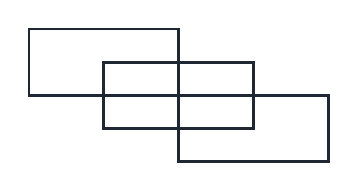
\begin{tikzpicture}[x=0.95cm,y=0.42cm]
\draw[Ink,line width=1pt] (0,2) rectangle (2,4);
\draw[Ink,line width=1pt] (1,1) rectangle (3,3);
\draw[Ink,line width=1pt] (2,0) rectangle (4,2);
\end{tikzpicture}
\end{minipage}
\end{probbox}
\probsol{
\textbf{Understanding the problem.} Call the three identical rectangles \textbf{I} (top left), \textbf{II} (middle) and \textbf{III} (bottom right). Where their sides cross, more small rectangles appear. We must count \emph{all} rectangles whose four sides are all drawn in the figure.
\step{1}{Look carefully at the figure}
Label the points as below. Notice: the bottom side of rectangle I and the top side of rectangle III lie on \emph{the same straight line} and join at the point $O$ -- the centre of rectangle II. Likewise the right side of I and the left side of III join at $O$. So inside rectangle II there is a ``plus sign'' that divides II into $4$ equal small cells.
\begin{center}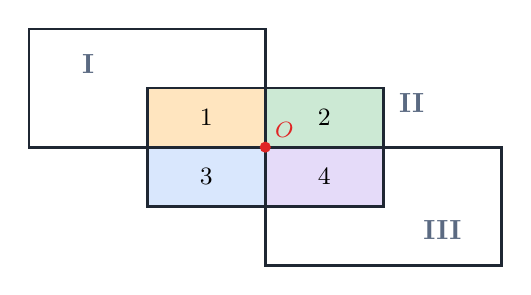
\begin{tikzpicture}[x=1.5cm,y=0.75cm,font=\sffamily\small]
\fill[tmOrange!25] (1,2) rectangle (2,3);\fill[tmGreen!25] (2,2) rectangle (3,3);
\fill[tmBlue!20] (1,1) rectangle (2,2);\fill[tmPurple!20] (2,1) rectangle (3,2);
\draw[Ink,line width=1pt] (0,2) rectangle (2,4);
\draw[Ink,line width=1pt] (1,1) rectangle (3,3);
\draw[Ink,line width=1pt] (2,0) rectangle (4,2);
\node at (1.5,2.5){$1$};\node at (2.5,2.5){$2$};\node at (1.5,1.5){$3$};\node at (2.5,1.5){$4$};
\fill[AnsRed] (2,2) circle (2pt);\node[above right,font=\footnotesize\bfseries,text=AnsRed] at (2,2){$O$};
\node[font=\bfseries,text=Slate] at (0.5,3.4){I};\node[font=\bfseries,text=Slate] at (3.5,0.6){III};
\node[font=\bfseries,text=Slate,anchor=west] at (3.05,2.75){II};
\end{tikzpicture}\end{center}
\step{2}{Count type by type}
\begin{itemize}[leftmargin=1.2em,itemsep=1pt,topsep=1pt]
\item \textbf{The three original large rectangles:} I, II, III -- $3$ rectangles.
\item \textbf{The four small cells} inside rectangle II (cells $1$, $2$, $3$, $4$) -- $4$ rectangles. Each cell has all four sides: for example cell $1$ has its top and left sides on rectangle II, and its bottom and right sides on rectangle I.
\item \textbf{Halves of rectangle II} (two neighbouring cells joined): cells $1+2$ (top half), $3+4$ (bottom half), $1+3$ (left half), $2+4$ (right half) -- $4$ rectangles.
\end{itemize}
\step{3}{Check that there are no others}
\begin{itemize}[leftmargin=1.2em,itemsep=1pt,topsep=1pt]
\item The part of rectangle I \emph{outside} rectangle II is L-shaped, and no segment passes through it. A rectangle containing part of this L-shaped region must use the left side and the top side of rectangle I as its sides; these two sides are exactly as long as the sides of rectangle I, so that rectangle is rectangle I itself. Likewise, a rectangle containing part of III outside II can only be rectangle III.
\item Every other rectangle must lie entirely inside rectangle II. Rectangle II with its inner ``plus sign'' is a $2\times2$ grid of cells, and in Step 2 we have listed them all: $4$ cells, $4$ halves and rectangle II itself.
\end{itemize}
\begin{warnbox}Do not count the large rectangle surrounding all three shapes (from the top-left corner of I to the bottom-right corner of III): \emph{none} of its sides is fully drawn. And do not miss the small cells created by the ``plus sign'' in the centre.\end{warnbox}
\step{4}{Add up}
$3+4+4=11$ rectangles.
\verify{Another count -- inside rectangle II alone (a complete $2\times2$ grid): by Example 7 there are $9$ rectangles ($4$ cells, $4$ halves and II itself). Adding rectangles I and III: $9+2=11$ \checkmark.}
The answer is \textbf{(A)}.
\ans{(A) $11$}
}

% ---------------- part b ----------------
% ================= Topic 3 (EN) -- part b: problems 16--30 =================
\providecommand{\cpTooth}[3]{% #1 rows, #2 columns, #3 unit (cm): grid of toothpicks
  \foreach \j in {0,...,#1}{\foreach \i in {1,...,#2}{
    \draw[tmOrange!85!black,line width=1.6pt,line cap=round]
      ({(\i-1)*#3+0.05},{\j*#3})--({\i*#3-0.05},{\j*#3});}}
  \foreach \j in {1,...,#1}{\foreach \i in {0,...,#2}{
    \draw[tmOrange!85!black,line width=1.6pt,line cap=round]
      ({\i*#3},{(\j-1)*#3+0.05})--({\i*#3},{\j*#3-0.05});}}}

\begin{probbox}{16}{\relax}
On the dot grid shown, Lan stands at dot $A$. She tosses a fair coin to decide how to move: if the coin shows
\emph{heads} she moves \emph{up} one dot; if it shows \emph{tails} she moves \emph{right} one dot. After exactly four
tosses, Lan will stop at one of the five dots $P$, $Q$, $R$, $S$, $T$. What is the probability that Lan stops at dot $R$?
\begin{figC}\begin{scope}[scale=0.8]
  \foreach \y in {0,...,4}{\pgfmathtruncatemacro\m{4-\y}
    \foreach \x in {0,...,\m}{\fill[Navy] (\x,\y) circle (2.6pt);}}
  \node[below left] at (0,0) {$A$};
  \node[above right] at (0,4) {$P$};\node[above right] at (1,3) {$Q$};
  \node[above right] at (2,2) {$R$};\node[above right] at (3,1) {$S$};
  \node[above right] at (4,0) {$T$};
  \fill[tmOrange] (0,0) circle (3.4pt);
\end{scope}\end{figC}
\choices{$\dfrac12$}{$\dfrac38$}{$\dfrac9{16}$}{$\dfrac7{16}$}{$\dfrac5{16}$}
\end{probbox}
\probsol{
\textbf{Understanding the problem.} At each toss Lan moves \emph{up} ($\uparrow$, for heads) or \emph{right}
($\rightarrow$, for tails). After $4$ tosses she has made exactly $4$ moves. We need the probability that after these
$4$ moves she is at $R$.

\step{1}{Count all possible outcomes}
Each toss has $2$ outcomes (heads or tails), so four tosses in a row give
$2\times2\times2\times2=16$ sequences, for example $\uparrow\rightarrow\rightarrow\uparrow$.
Since the coin is fair, these $16$ sequences are \emph{equally likely}.
\begin{recallbox}\emph{Multiplication principle:} if the first task can be done in $a$ ways, the second in $b$ ways, \dots{} then
doing them one after another can be done in $a\times b\times\cdots$ ways. The \emph{probability} of an event (when the outcomes
are equally likely) $=\dfrac{\text{number of favourable outcomes}}{\text{number of possible outcomes}}$.\end{recallbox}

\step{2}{The final dot depends only on the number of up-moves}
If $k$ of the $4$ moves are up, then $4-k$ moves are to the right. The order of the moves does not change the final dot.
Starting from $A$: $4$ ups $\to P$; $3$ ups $\to Q$; $2$ ups $\to R$; $1$ up $\to S$; $0$ ups $\to T$.
So Lan stops at $R$ exactly when she makes \textbf{exactly $2$ moves up and $2$ moves right}.

\step{3}{List the favourable sequences}
We choose which two of the four turns (turn 1, 2, 3, 4) are $\uparrow$:
\[\uparrow\uparrow\rightarrow\rightarrow,\quad \uparrow\rightarrow\uparrow\rightarrow,\quad
\uparrow\rightarrow\rightarrow\uparrow,\quad \rightarrow\uparrow\uparrow\rightarrow,\quad
\rightarrow\uparrow\rightarrow\uparrow,\quad \rightarrow\rightarrow\uparrow\uparrow.\]
There are $6$ sequences (choosing $2$ turns out of $4$: $\dfrac{4\times3}{2}=6$ ways).

\step{4}{Compute the probability}
\[P(\text{stop at } R)=\frac{6}{16}=\frac38.\]

\step{5}{A picture: write the number of paths at each dot}
At each dot write the number of move sequences leading from $A$ to that dot. A dot can only be reached from the dot just to its
left or the dot just below it, so the number at each dot $=$ the sum of the numbers to its left and below (just like Pascal's triangle):
\begin{figC}\begin{scope}[scale=0.75]
  \foreach \x/\y/\n in {0/0/1,1/0/1,2/0/1,3/0/1,4/0/1,0/1/1,1/1/2,2/1/3,3/1/4,0/2/1,1/2/3,2/2/6,
     0/3/1,1/3/4,0/4/1}{
    \fill[tmBlue!12] (\x,\y) circle (9pt);
    \node[font=\small\bfseries,text=Navy] at (\x,\y) {\n};}
  \draw[AnsRed,thick] (2,2) circle (10pt);
  \node[right=10pt,text=AnsRed,font=\small] at (2,2) {$R$};
  \node[right=10pt,font=\small] at (4,0) {$T$};\node[right=10pt,font=\small] at (3,1) {$S$};
  \node[right=10pt,font=\small] at (1,3) {$Q$};\node[right=10pt,font=\small] at (0,4) {$P$};
\end{scope}\end{figC}
Along the last diagonal: $1+4+6+4+1=16$ (exactly the total number of sequences), and the number at $R$ is $6$.
\begin{warnbox}The five dots $P,Q,R,S,T$ are \emph{not} equally likely! Do not answer ``one of $5$ dots, so the probability is
$\frac15$''. The middle dot ($R$) can be reached in the most ways; each of the two end dots ($P$ and $T$) can be reached in only one way.\end{warnbox}
\verify{The probabilities of stopping at $P,Q,R,S,T$ are $\frac1{16},\frac4{16},\frac6{16},\frac4{16},\frac1{16}$;
they add up to $\frac{16}{16}=1$, as they should.}
The value $\frac38=\frac6{16}$ is option \textbf{(B)}.
\ans{(B) $\dfrac38$}
}

\begin{probbox}{17}{\relax}
Identical toothpicks are used to build rectangular grids of squares, as shown below. For example, the $1\times10$ grid
($1$ row of $10$ squares) uses $31$ toothpicks in total. How many toothpicks are needed for a $43\times10$ grid
($43$ rows, each with $10$ squares)?
\begin{figC}
  \begin{scope}[shift={(0,2.4)}]\cpTooth{1}{10}{0.42}\node[right] at (4.4,0.21) {$1\times10$};\end{scope}
  \begin{scope}[shift={(0,1.05)}]\cpTooth{2}{10}{0.42}\node[right] at (4.4,0.42) {$2\times10$};\end{scope}
  \begin{scope}[shift={(0,-0.6)}]\cpTooth{3}{10}{0.42}\node[right] at (4.4,0.63) {$3\times10$};\end{scope}
\end{figC}
\choices{$913$}{$860$}{$871$}{$903$}{$946$}
\end{probbox}
\probsol{
\textbf{Understanding the problem.} The $43\times10$ grid has $43$ rows of squares, $10$ squares in each row. The toothpicks lie in
two directions: \emph{horizontal} and \emph{vertical}. We count each kind separately and add (addition principle).

\step{1}{Check the method on the $1\times10$ grid}
\emph{Horizontal toothpicks:} the grid has $2$ horizontal lines (top edge and bottom edge), each made of $10$ toothpicks:
$2\times10=20$ toothpicks.
\emph{Vertical toothpicks:} there are $11$ vertical lines ($10$ squares need $11$ walls), each made of $1$ toothpick:
$11\times1=11$ toothpicks. Total: $20+11=31$, exactly as stated.
\begin{recallbox}A row of $10$ squares needs $10+1=11$ vertical walls (like the fence-post problem: $10$ gaps need $11$ posts).
In the same way, $43$ rows of squares have $43+1=44$ horizontal lines.\end{recallbox}

\step{2}{Count the horizontal toothpicks of the $43\times10$ grid}
There are $43+1=44$ horizontal lines, each $10$ toothpicks long: $44\times10=440$ toothpicks.

\step{3}{Count the vertical toothpicks of the $43\times10$ grid}
There are $10+1=11$ vertical lines, each $43$ toothpicks long (one toothpick per row): $11\times43=473$ toothpicks.

\step{4}{Add}
$440+473=913$ toothpicks.

\step{5}{Second method: add one row at a time}
The $1\times10$ grid has $31$ toothpicks. Each time a new row is placed on top, we need $10$ more horizontal toothpicks
(the top edge of the new row) and $11$ vertical ones, that is $21$ toothpicks (the bottom edge is already there). Going from
$1$ row to $43$ rows means adding $42$ rows:
\[31+42\times21=31+882=913.\]
\begin{warnbox}Do not compute $43\times31=1333$: when rows are stacked, two neighbouring rows \emph{share} a line of $10$ horizontal
toothpicks, so multiplying like that counts those toothpicks twice.\end{warnbox}
\verify{By the formula $(\text{rows}+1)\times10+11\times\text{rows}$: the $2\times10$ grid needs
$3\times10+11\times2=52$ toothpicks and the $3\times10$ grid needs $4\times10+11\times3=73$; counting directly in the picture also gives
$52$ and $73$. Both methods give the same result, $913$.}
So the answer is \textbf{(A)}.
\ans{(A) $913$ toothpicks}
}

\begin{probbox}{18}{\relax}
In the cafeteria at Minh's school, the meats are beef and chicken, and the fruits are apple, pear and banana. Minh is given a
random lunch consisting of one meat and one fruit. The probability that Minh's lunch includes a banana is
\choices{$\dfrac13$}{$\dfrac23$}{$\dfrac12$}{$\dfrac15$}{$\dfrac35$}
\end{probbox}
\probsol{
\textbf{Understanding the problem.} A lunch $=$ (one meat, one fruit). The lunch is chosen at random, so all possible lunches are
equally likely. We need the probability that the lunch includes a banana.

\step{1}{List all possible lunches}
By the multiplication principle there are $2\times3=6$ lunches. We make a table (rows: meat, columns: fruit):
\begin{center}\begin{tabular}{|c|c|c|c|}\hline
 & Apple & Pear & \cellcolor{tmOrange!20}Banana\\\hline
Beef & Beef--Apple & Beef--Pear & \cellcolor{tmOrange!20}Beef--Banana\\\hline
Chicken & Chicken--Apple & Chicken--Pear & \cellcolor{tmOrange!20}Chicken--Banana\\\hline
\end{tabular}\end{center}

\step{2}{Count the lunches with a banana}
The ``Banana'' column has $2$ lunches: Beef--Banana and Chicken--Banana.

\step{3}{Compute the probability}
\[P(\text{banana})=\frac{2}{6}=\frac13.\]
\begin{recallbox}To simplify a fraction, divide the numerator and the denominator by their greatest common divisor:
$\dfrac26=\dfrac{2\div2}{6\div2}=\dfrac13$.\end{recallbox}
\begin{tipbox}The meat has no effect on the fruit. A quicker way to think: the fruit is one of $3$ equally likely kinds, and banana is
$1$ of the $3$ kinds, so the probability is $\frac13$.\end{tipbox}
\begin{warnbox}Do not add ``$2$ meats $+\,3$ fruits $=5$'' and answer $\frac15$: the number of lunches is $2\times3=6$, not $2+3=5$.\end{warnbox}
\verify{The probabilities of getting an apple, a pear and a banana are all $\frac13$; they add up to $\frac13+\frac13+\frac13=1$.}
So the answer is \textbf{(A)}.
\ans{(A) $\dfrac13$}
}

\begin{probbox}{19}{\relax}
A special six-sided die is made, with one number written on each face (numbers may repeat). When this die is rolled, the probability
of getting a multiple of $3$ is $\frac12$, and the probability of getting an even number is $\frac13$.
The six numbers on the faces could be
\choicesII{$1,2,3,5,5,6$}{$1,2,3,3,5,6$}{$1,2,3,4,6,6$}{$1,2,3,3,4,6$}{$2,3,3,3,5,6$}
\end{probbox}
\probsol{
\textbf{Understanding the problem.} The die has $6$ equally likely faces. From the two given probabilities we work out the
\emph{number of faces} showing a multiple of $3$ and the number of faces showing an even number, then check each option.

\step{1}{Turn probabilities into numbers of faces}
\begin{recallbox}With $6$ equally likely faces: $P=\dfrac{\text{number of favourable faces}}{6}$, so
the number of favourable faces $=P\times6$.\end{recallbox}
Faces with a multiple of $3$: $\frac12\times6=3$ faces.\quad Even faces: $\frac13\times6=2$ faces.

So we need: \textbf{exactly $3$ faces that are multiples of $3$} and \textbf{exactly $2$ even faces}.

\step{2}{Check each option}
Among the numbers $1$ to $6$: the multiples of $3$ are $3$ and $6$; the even numbers are $2$, $4$, $6$.
Note that $6$ is both even and a multiple of $3$, so it must be counted in \emph{both} columns.
\begin{center}\begin{tabular}{|c|c|c|c|c|}\hline
Option & Faces & Multiples of $3$ & Even faces & OK?\\\hline
(A) & $1,2,3,5,5,6$ & $3,6$ \;($2$ faces) & $2,6$ \;($2$ faces) & No\\\hline
\rowcolor{tmGreen!12}(B) & $1,2,3,3,5,6$ & $3,3,6$ \;($3$ faces) & $2,6$ \;($2$ faces) & Yes\\\hline
(C) & $1,2,3,4,6,6$ & $3,6,6$ \;($3$ faces) & $2,4,6,6$ \;($4$ faces) & No\\\hline
(D) & $1,2,3,3,4,6$ & $3,3,6$ \;($3$ faces) & $2,4,6$ \;($3$ faces) & No\\\hline
(E) & $2,3,3,3,5,6$ & $3,3,3,6$ \;($4$ faces) & $2,6$ \;($2$ faces) & No\\\hline
\end{tabular}\end{center}
\begin{warnbox}If you forget that $6$ is even, you will count only $2$ even faces for (D) and wrongly choose (D).
A number can belong to several groups at once!\end{warnbox}
\verify{For (B): $P(\text{multiple of }3)=\frac36=\frac12$ and $P(\text{even})=\frac26=\frac13$; both conditions hold.}
Only option \textbf{(B)} works.
\ans{(B) $1,2,3,3,5,6$}
}

\begin{probbox}{20}{\stars{1}}
Three bus routes run along the roads shown in the figure, all passing through stop $X$ (segments with the same number of small marks
are equal: $PX=XS$, $QX=XT$, $RX=XU$).
\begin{itemize}[leftmargin=1.2em,itemsep=1pt,topsep=2pt]
\item Bus $A$ runs the route $P\to X\to S\to X\to P$; each round trip takes $12$ minutes.
\item Bus $B$ runs the route $Q\to X\to T\to X\to Q$; each round trip takes $20$ minutes.
\item Bus $C$ runs the route $R\to X\to U\to X\to R$; each round trip takes $28$ minutes.
\end{itemize}
At 1:00 p.m., buses $A$, $B$, $C$ leave $P$, $Q$, $R$ respectively. Each bus travels at a constant speed, turns around instantly
at both ends of its route and runs without stopping until 11:00 p.m. Between 5:00 p.m. and 10:00 p.m., at how many moments are two
or more buses at stop $X$ at the same time?
\begin{figC}\begin{scope}[scale=0.9]
  \draw[Ink,thick] (0,1.6)--(0,-1.6);\draw[Ink,thick] (-1.9,0)--(1.9,0);\draw[Ink,thick] (-2,-1.35)--(2,1.35);
  \foreach \p in {(0,1.6),(0,-1.6),(-1.9,0),(1.9,0),(-2,-1.35),(2,1.35),(0,0)}{\fill[Navy] \p circle (2pt);}
  \node[above] at (0,1.6) {$P$};\node[below] at (0,-1.6) {$S$};\node[left] at (-1.9,0) {$Q$};
  \node[right] at (1.9,0) {$T$};\node[below left] at (-2,-1.35) {$R$};\node[above right] at (2,1.35) {$U$};
  \node[below right] at (0.05,-0.02) {$X$};
  \draw[tmBlue,thick] (-0.12,0.8)--(0.12,0.8);\draw[tmBlue,thick] (-0.12,-0.8)--(0.12,-0.8);
  \foreach \s in {-1,1}{\draw[tmOrange,thick] (\s*0.95-0.04,-0.12)--(\s*0.95-0.04,0.12);
                        \draw[tmOrange,thick] (\s*0.95+0.04,-0.12)--(\s*0.95+0.04,0.12);}
  \foreach \s in {-1,1}{\foreach \d in {-0.09,0,0.09}{
     \draw[tmGreen!80!black,thick] ($(\s*1,\s*0.675)+(\d*0.829,\d*0.559)+(0.067,-0.1)$)--++(-0.134,0.2);}}
\end{scope}\end{figC}
\choices{$18$}{$19$}{$20$}{$21$}{$22$}
\end{probbox}
\probsol{
\textbf{Understanding the problem.} We measure time as \emph{the number of minutes after 1:00 p.m.} and call this number $t$.
We need the values of $t$ at which at least two buses are at $X$, with $t$ between 5:00 p.m. and 10:00 p.m.

\step{1}{Convert the time window into minutes}
5:00 p.m. is $4$ hours after 1:00 p.m.: $t=4\times60=240$. \quad 10:00 p.m. is $9$ hours after 1:00 p.m.: $t=9\times60=540$.
So we look at $240\le t\le540$.

\step{2}{When is bus $A$ at $X$?}
One round trip of bus $A$ consists of $4$ equal legs: $P\to X$, $X\to S$, $S\to X$, $X\to P$ (because $PX=XS$).
The bus moves at constant speed, so each leg takes $12\div4=3$ minutes. Bus $A$ reaches $X$ at the end of the first leg and at the end
of the third leg of every round trip, that is at
\[t=3,\ 9,\ 15,\ 21,\ 27,\ \dots\]
These are exactly the \textbf{odd multiples of $3$} ($3\times1$, $3\times3$, $3\times5$, \dots). At the end of the second and fourth legs
the bus is at $S$ or $P$, not at $X$.

\step{3}{The same for buses $B$ and $C$}
Bus $B$: each leg takes $20\div4=5$ minutes, so it is at $X$ when $t=5,15,25,35,\dots$ -- the \textbf{odd multiples of $5$}.\\
Bus $C$: each leg takes $28\div4=7$ minutes, so it is at $X$ when $t=7,21,35,49,\dots$ -- the \textbf{odd multiples of $7$}.

\step{4}{When do two buses meet at $X$?}
\begin{recallbox}A number divisible by both $3$ and $5$ is divisible by $\text{lcm}(3,5)=15$. Similarly:
divisible by both $3$ and $7$ $\Leftrightarrow$ divisible by $21$; divisible by both $5$ and $7$ $\Leftrightarrow$
divisible by $35$.\end{recallbox}
Buses $A$ and $B$ are both at $X$ when $t$ is an odd multiple of $3$ and also an odd multiple of $5$, that is when $t$ is an
\textbf{odd number divisible by $15$} (an odd multiple of $15$). Similarly: $A$ and $C$ meet when $t$ is an odd multiple of $21$;
$B$ and $C$ meet when $t$ is an odd multiple of $35$.
\begin{proofbox}An odd multiple of $15$ is an odd number divisible by $15$, so it is an odd number divisible by $3$ (an odd multiple of $3$)
and an odd number divisible by $5$ (an odd multiple of $5$). Conversely, a number that is an odd multiple of $3$ and an odd multiple of $5$ is
odd and divisible by $15$.\end{proofbox}

\step{5}{List them for $240\le t\le540$}
\begin{center}\begin{tabular}{|l|l|c|}\hline
Two buses & Values of $t$ (odd multiples) & Count\\\hline
$A$ and $B$ ($15$) & $255, 285, 315, 345, 375, 405, 435, 465, 495, 525$ & $10$\\\hline
$A$ and $C$ ($21$) & $273, 315, 357, 399, 441, 483, 525$ & $7$\\\hline
$B$ and $C$ ($35$) & $245, 315, 385, 455, 525$ & $5$\\\hline
\end{tabular}\end{center}
(For example, in the first row: $15\times17=255$ is the first odd multiple greater than $240$; after that we keep adding $30$, because
two consecutive odd multiples of $15$ are $2\times15=30$ apart.)

\step{6}{Remove the moments counted more than once}
Adding the three rows gives $10+7+5=22$, but the moments $315$ and $525$ appear in \emph{all three rows}
(they are odd multiples of $3\times5\times7=105$: at those moments all three buses are at $X$). Each of these moments is counted $3$ times
but should be counted only once, so we subtract $2+2=4$:
\[22-4=18 \text{ moments.}\]
\begin{warnbox}The question asks for the number of \emph{moments}, not the number of ``pairs of buses meeting''. When all three buses are at
$X$ together, that is just \emph{one} moment. Adding $10+7+5=22$ and choosing (E) is wrong.\end{warnbox}
\verify{In clock times: 5:05, 5:15, 5:33, 5:45, 6:15, 6:45, 6:57, 7:15, 7:25, 7:39, 7:45, 8:15, 8:21, 8:35, 8:45, 9:03, 9:15, 9:45 p.m.
-- exactly $18$ moments, all between 5:00 p.m. and 10:00 p.m.}
So the answer is \textbf{(A)}.
\ans{(A) $18$}
}

\begin{probbox}{21}{\relax}
Each face of a cube is painted with exactly one colour. What is the smallest number of colours needed to paint the cube so that any
two faces sharing an edge have different colours?
\choices{$2$}{$3$}{$4$}{$5$}{$6$}
\end{probbox}
\probsol{
\textbf{Understanding the problem.} Two faces ``sharing an edge'' are adjacent faces. Two opposite faces (such as the top and the
bottom) have no common edge, so they may have the same colour. We must (1) show a colouring that uses few colours, and
(2) prove that fewer colours are impossible.

\step{1}{Two colours are not enough}
\begin{proofbox}Look at any corner of the cube, for example the top--front--right corner. Three faces meet there: the top, the front and the
right face. Any two of these three faces share an edge, so the three faces must have three different colours. Hence at least $3$ colours
are needed.\end{proofbox}

\step{2}{Three colours are enough}
Paint \emph{each pair of opposite faces the same colour}: top and bottom blue, front and back orange, left and right green.
Each face is adjacent to $4$ faces, which are exactly the four faces \emph{not} opposite to it, and these four faces carry the other two
colours. So no two adjacent faces have the same colour.
\begin{figC}
  \begin{scope}
   \fill[tmOrange!55,draw=Ink,thick] (0,0)--(1.6,0)--(1.6,1.6)--(0,1.6)--cycle;
   \fill[tmBlue!55,draw=Ink,thick] (0,1.6)--(1.6,1.6)--(2.4,2.3)--(0.8,2.3)--cycle;
   \fill[tmGreen!55,draw=Ink,thick] (1.6,0)--(2.4,0.7)--(2.4,2.3)--(1.6,1.6)--cycle;
   \node at (0.8,0.8) {front};\node at (1.2,1.95) {top};\node at (2,1.15) {right};
  \end{scope}
  \begin{scope}[shift={(4,0.1)},scale=0.5]
   \foreach \x/\y/\c in {1/2/tmBlue,0/1/tmGreen,1/1/tmOrange,2/1/tmGreen,3/1/tmOrange,1/0/tmBlue}{
     \fill[\c!55,draw=Ink,thick] (\x,\y) rectangle ++(1,1);}
   \node[font=\scriptsize] at (2,-0.45) {net of the cube};
  \end{scope}
\end{figC}

\step{3}{Conclusion}
At least $3$ colours are needed (step 1) and $3$ colours are enough (step 2), so the smallest number of colours is $3$.
\begin{warnbox}Finding one colouring with $3$ colours is \emph{not enough} to claim that $3$ is the smallest; you must explain why $2$ colours
fail (the three faces at a corner). On the other hand, thinking ``$6$ faces need $6$ colours'' forgets that opposite faces may share a
colour.\end{warnbox}
\verify{On the net, each square shares edges only with squares of other colours (when folded, two squares of the same colour become
opposite faces).}
So the answer is \textbf{(B)}.
\ans{(B) $3$ colours}
}

\begin{probbox}{22}{\relax}
How many different pairs $(m,n)$ can be formed from the integers $1,2,3,\dots,20$ such that $m<n$ and $m+n$ is even?
\choices{$55$}{$90$}{$140$}{$110$}{$50$}
\end{probbox}
\probsol{
\textbf{Understanding the problem.} We choose two different numbers out of $20$; because $m<n$, each pair of two numbers is counted
\emph{only once} (the smaller one is $m$, the larger one is $n$). Condition: the sum $m+n$ is even.

\step{1}{When is the sum of two numbers even?}
\begin{recallbox}even $+$ even $=$ even;\quad odd $+$ odd $=$ even;\quad even $+$ odd $=$ odd.\end{recallbox}
So $m+n$ is even exactly when $m$ and $n$ have \textbf{the same parity} (both even or both odd).

\step{2}{Split the $20$ numbers into two groups}
Even group: $2,4,6,\dots,20$ -- $10$ numbers.\quad Odd group: $1,3,5,\dots,19$ -- $10$ numbers.

\step{3}{Count the pairs in the even group}
The first number can be chosen in $10$ ways and the second (different from the first) in $9$ ways: $10\times9=90$ \emph{ordered} choices.
But each pair, for example $\{2,4\}$, is counted twice ($2$ then $4$, or $4$ then $2$), while the condition $m<n$ allows only the order
$(2,4)$. So the number of pairs is $\dfrac{10\times9}{2}=45$.
\begin{recallbox}The number of ways to choose $2$ objects (order does not matter) from $k$ objects is $\dfrac{k\times(k-1)}{2}$.\end{recallbox}

\step{4}{Count the pairs in the odd group and add}
In the same way the odd group gives $45$ pairs. A pair cannot be in both groups, so by the addition principle:
$45+45=90$ pairs.
\begin{warnbox}Forgetting to divide by $2$ gives $90+90=180$ (not an option); forgetting the odd group gives $45$. Always ask yourself:
``Did I count a pair twice? Did I miss a case?''\end{warnbox}
\verify{Count using the complement: the total number of pairs with $m<n$ is $\dfrac{20\times19}{2}=190$. The number of pairs with different
parity (one even, one odd) is $10\times10=100$. So the number of pairs with the same parity is $190-100=90$. It matches!}
So the answer is \textbf{(B)}.
\ans{(B) $90$ pairs}
}

\begin{probbox}{23}{\stars{1}}
Two different two-digit positive integers are called a \emph{reversal pair} if one is obtained from the other by swapping its two digits.
For example, $52$ and $25$ form a reversal pair. The number $2015$ has a special property: it is the product of three different prime
numbers, two of which form a reversal pair ($2015=5\times13\times31$). Including $2015$, how many positive integers less than $10\,000$
have this same property?
\choices{$18$}{$14$}{$20$}{$17$}{$19$}
\end{probbox}
\probsol{
\textbf{Understanding the problem.} We must count the numbers $N<10\,000$ of the form $N=p\times q\times r$, where $p,q,r$ are three
different primes and two of them (call them $p$ and $q$) form a two-digit reversal pair. Plan: find all reversal pairs made of two primes,
then for each pair find the suitable third primes.

\step{1}{Find the reversal pairs in which both numbers are prime}
\begin{recallbox}A prime number is a natural number greater than $1$ whose only divisors are $1$ and itself. The two-digit primes are:
$11, 13, 17, 19, 23, 29, 31, 37, 41, 43, 47, 53, 59, 61, 67, 71, 73, 79, 83, 89, 97$.\end{recallbox}
\begin{tipbox}The units digit of the reversal of $p$ is the tens digit of $p$. A two-digit prime must end in $1,3,7$ or $9$, so we only need
to look at primes starting with $1,3,7,9$: $11,13,17,19,31,37,71,73,79,97$.\end{tipbox}
Check the reversal of each one:
\begin{center}\begin{tabular}{|c|c|c|c|c|c|c|c|c|c|c|}\hline
$p$ & $11$ & $13$ & $17$ & $19$ & $31$ & $37$ & $71$ & $73$ & $79$ & $97$\\\hline
reversal & $11$ & $31$ & $71$ & $91$ & $13$ & $73$ & $17$ & $37$ & $97$ & $79$\\\hline
prime? & same & yes & yes & no & yes & yes & yes & yes & yes & yes\\\hline
\end{tabular}\end{center}
($91=7\times13$ is not prime; $11$ reversed is still $11$, so it does not give two \emph{different} numbers.)
So there are exactly $4$ pairs: $\{13,31\}$, $\{17,71\}$, $\{37,73\}$, $\{79,97\}$.

\step{2}{Compute the product of each pair}
$13\times31=403$;\quad $17\times71=1207$;\quad $37\times73=2701$;\quad $79\times97=7663$.

\step{3}{Find the third prime $r$ for each pair}
We need $r$ prime, different from the two numbers of the pair, and the product $<10\,000$.
\begin{itemize}[leftmargin=1.2em,itemsep=1pt,topsep=2pt]
\item Pair $\{13,31\}$: we need $403\times r<10\,000$. Since $403\times24=9672$ and $403\times25=10\,075$, we need $r\le23$.
The primes $\le23$ are $2,3,5,7,11,13,17,19,23$; remove $13$ (already in the pair): $8$ primes remain, giving
$806;\ 1209;\ 2015;\ 2821;\ 4433;\ 6851;\ 7657;\ 9269$.
\item Pair $\{17,71\}$: we need $1207\times r<10\,000$; since $1207\times8=9656$ and $1207\times9=10\,863$, $r\le8$:
$r\in\{2,3,5,7\}$, giving $2414;\ 3621;\ 6035;\ 8449$ ($4$ numbers).
\item Pair $\{37,73\}$: $2701\times3=8103<10\,000$ and $2701\times4>10\,000$, so $r\in\{2,3\}$: $5402;\ 8103$ ($2$ numbers).
\item Pair $\{79,97\}$: even $7663\times2=15\,326>10\,000$, so there are none.
\end{itemize}

\step{4}{Check that no number is counted twice, and add}
\begin{proofbox}Every number has only one prime factorisation. If a number appeared in two lists, then among its three prime factors there
would be two different reversal pairs; these two pairs would have to share a prime. But the table in step 1 shows that each prime belongs
to exactly one pair. So no number is counted twice.\end{proofbox}
In total: $8+4+2+0=14$ numbers.
\begin{warnbox}Two common mistakes: (1) forgetting that the third prime must be \emph{different} from the two primes of the pair, and so
also counting $403\times13=5239=13\times13\times31$ (wrong, since $13$ is repeated); (2) forgetting the prime $2$.\end{warnbox}
\verify{$2015=403\times5$ is in the list. Checking a few numbers: $9269=13\times31\times23$, $8449=17\times71\times7$,
$8103=37\times73\times3$; all are less than $10\,000$.}
So the answer is \textbf{(B)}.
\ans{(B) $14$}
}

\begin{probbox}{24}{\relax}
The figure is made of $8$ identical small parallelograms. Including these $8$ small parallelograms, how many parallelograms are there in
the figure altogether?
\begin{figC}
  \foreach \j in {0,1,2}{\draw[Ink,thick] (\j*0.55,\j*0.8)--(4.4+\j*0.55,\j*0.8);}
  \foreach \i in {0,...,4}{\draw[Ink,thick] (\i*1.1,0)--(\i*1.1+1.1,1.6);}
\end{figC}
\choices{$29$}{$30$}{$26$}{$27$}{$28$}
\end{probbox}
\probsol{
\textbf{Understanding the problem.} The figure has $2$ rows, each with $4$ small parallelograms. Every parallelogram in the figure is
formed from the segments already drawn: two of its sides lie on \emph{horizontal lines} and two lie on \emph{slanted lines}.

\step{1}{Count the lines in the figure}
There are $3$ horizontal lines (bottom, middle, top) and $5$ slanted lines (parallel to each other).
\begin{figC}
  \foreach \j/\l in {0/1,1/2,2/3}{\draw[tmBlue,thick] (\j*0.55,\j*0.8)--(4.4+\j*0.55,\j*0.8);
     \node[left,text=tmBlue,font=\scriptsize] at (\j*0.55,\j*0.8) {horiz.\ \l};}
  \foreach \i in {0,...,4}{\draw[tmOrange,thick] (\i*1.1,0)--(\i*1.1+1.1,1.6);
     \pgfmathtruncatemacro\k{\i+1}\node[below,text=tmOrange!80!black,font=\scriptsize] at (\i*1.1,0) {s\k};}
  \fill[tmGreen!30,opacity=0.7] (1.1,0)--(3.3,0)--(3.85,0.8)--(1.65,0.8)--cycle;
\end{figC}
For example, the green parallelogram is determined by horizontal lines $1$ and $2$ and slanted lines s$2$ and s$4$.

\step{2}{Each parallelogram corresponds to a choice of $2$ horizontal lines and $2$ slanted lines}
Choosing $2$ of the $3$ horizontal lines as bottom and top sides, and $2$ of the $5$ slanted lines as left and right sides, gives exactly
one parallelogram; conversely, every parallelogram in the figure comes from exactly one such choice.
\begin{recallbox}The number of ways to choose $2$ lines out of $k$ lines is $\dfrac{k\times(k-1)}{2}$.\end{recallbox}
Choosing $2$ horizontal lines: $\dfrac{3\times2}{2}=3$ ways. \quad Choosing $2$ slanted lines: $\dfrac{5\times4}{2}=10$ ways.

\step{3}{Apply the multiplication principle}
Number of parallelograms: $3\times10=30$.

\step{4}{Check by counting by size}
Call a parallelogram ``height $a$, width $b$'' if it is made of $a$ rows and $b$ columns of small ones:
\begin{center}\begin{tabular}{|c|c|c|c|c|c|}\hline
 & width $1$ & width $2$ & width $3$ & width $4$ & Total\\\hline
height $1$ ($2$ positions in rows) & $2\times4=8$ & $2\times3=6$ & $2\times2=4$ & $2\times1=2$ & $20$\\\hline
height $2$ ($1$ position in rows) & $4$ & $3$ & $2$ & $1$ & $10$\\\hline
\end{tabular}\end{center}
\begin{warnbox}Do not just count the $8$ small ones plus a few ``obvious'' big ones. Count systematically: by size (table above) or by
choosing lines.\end{warnbox}
\verify{The table gives $20+10=30$, the same as $3\times10$.}
So the answer is \textbf{(B)}.
\ans{(B) $30$ parallelograms}
}

\begin{probbox}{25}{\stars{1}}
A jar contains $2$ red marbles and $2$ blue marbles and no other marbles. Hoa randomly takes $2$ marbles out of the jar at the same time.
If the two marbles have the same colour, she throws one away and puts the other back into the jar. If they have different colours, she
throws away the red marble and puts the blue marble back into the jar. Hoa does this three times in total. The probability that the last
marble left in the jar is red is
\choices{$\dfrac12$}{$\dfrac14$}{$\dfrac23$}{$\dfrac13$}{$0$}
\end{probbox}
\probsol{
\textbf{Understanding the problem.} Each draw removes exactly $1$ marble from the jar. After $3$ draws, $1$ of the $4$ marbles is left.
We follow the \emph{state} of the jar, written (number of red, number of blue), starting from $(2\text{R},2\text{B})$.

\step{1}{First draw, from $(2\text{R},2\text{B})$}
Call the marbles R$_1$, R$_2$, B$_1$, B$_2$. There are $6$ equally likely ways to take $2$ marbles:
R$_1$R$_2$;\ B$_1$B$_2$;\ R$_1$B$_1$;\ R$_1$B$_2$;\ R$_2$B$_1$;\ R$_2$B$_2$.
\begin{itemize}[leftmargin=1.2em,itemsep=1pt,topsep=2pt]
\item Two reds ($1$ way): throw away $1$ red $\to(1\text{R},2\text{B})$.
\item Two blues ($1$ way): throw away $1$ blue $\to(2\text{R},1\text{B})$.
\item Different colours ($4$ ways): throw away the red $\to(1\text{R},2\text{B})$.
\end{itemize}
So after draw $1$: state $(1\text{R},2\text{B})$ with probability $\frac56$, state $(2\text{R},1\text{B})$ with probability $\frac16$.

\step{2}{Second draw}
From $(1\text{R},2\text{B})$: $3$ ways to draw; $2$ ways give different colours $\to(0\text{R},2\text{B})$; $1$ way gives two blues $\to(1\text{R},1\text{B})$.\\
From $(2\text{R},1\text{B})$: $3$ ways to draw; $1$ way gives two reds $\to(1\text{R},1\text{B})$; $2$ ways give different colours $\to(1\text{R},1\text{B})$.
So from $(2\text{R},1\text{B})$ we certainly go to $(1\text{R},1\text{B})$.

\step{3}{Third draw}
From $(0\text{R},2\text{B})$: two blues are drawn, one is thrown away $\to(0\text{R},1\text{B})$.\\
From $(1\text{R},1\text{B})$: different colours are drawn, the red is thrown away $\to(0\text{R},1\text{B})$.
\begin{figC}
  \tikzset{st/.style={draw=tmBlue,fill=tmBlue!8,rounded corners=3pt,inner sep=3pt,font=\footnotesize}}
  \node[st] (a) at (0,0) {$2$R, $2$B};
  \node[st] (b) at (2.8,0.9) {$1$R, $2$B};\node[st] (c) at (2.8,-0.9) {$2$R, $1$B};
  \node[st] (d) at (5.6,0.9) {$0$R, $2$B};\node[st] (e) at (5.6,-0.9) {$1$R, $1$B};
  \node[st,draw=AnsRed,fill=AnsRed!8] (f) at (8.2,0) {$0$R, $1$B};
  \draw[->,thick,Slate] (a)--node[above,font=\scriptsize]{$\frac56$}(b);
  \draw[->,thick,Slate] (a)--node[below,font=\scriptsize]{$\frac16$}(c);
  \draw[->,thick,Slate] (b)--node[above,font=\scriptsize]{$\frac23$}(d);
  \draw[->,thick,Slate] (b)--node[above right,font=\scriptsize,pos=0.3]{$\frac13$}(e);
  \draw[->,thick,Slate] (c)--node[below,font=\scriptsize]{$1$}(e);
  \draw[->,thick,Slate] (d)--node[above,font=\scriptsize]{$1$}(f);
  \draw[->,thick,Slate] (e)--node[below,font=\scriptsize]{$1$}(f);
  \node[font=\scriptsize,text=Slate] at (1.4,-1.7) {draw 1};\node[font=\scriptsize,text=Slate] at (4.2,-1.7) {draw 2};
  \node[font=\scriptsize,text=Slate] at (6.9,-1.7) {draw 3};
\end{figC}
Every branch ends at $(0\text{R},1\text{B})$: the last marble is \textbf{always} blue.

\step{4}{Why -- without drawing the tree}
\begin{proofbox}Look at the number of blue marbles. Whenever at least one of the two marbles drawn is blue, Hoa always puts a blue marble back
into the jar (two blues: she puts one back; different colours: she puts the blue back). The number of blue marbles decreases only when two
blues are drawn, and then the one that was put back is still there. So the jar \emph{always contains at least one blue marble}. When only one
marble is left, it must be blue.\end{proofbox}
Therefore the event ``the last marble is red'' is an \emph{impossible event}, with probability $0$.
\begin{recallbox}An impossible event (one that never happens) has probability $0$; a certain event has probability $1$.\end{recallbox}
\begin{warnbox}Seeing ``$2$ red, $2$ blue'' and immediately guessing $\frac12$ is a trap: the throwing-away rule is \emph{not symmetric}
in the two colours (with different colours, the red one is always thrown away).\end{warnbox}
\verify{Total probability of reaching the final state $(0\text{R},1\text{B})$: $\frac56\cdot\frac23+\frac56\cdot\frac13+\frac16\cdot1=\frac{10}{18}+\frac{5}{18}+\frac{3}{18}=1$.}
So the answer is \textbf{(E)}.
\ans{(E) $0$}
}

\begin{probbox}{26}{\stars{1}}
On the $10\times10$ grid of squares shown, triangle $FGH$ is drawn. Point $P$ can be any of the $41$ points where grid lines cross
that lie \emph{inside} (not on the sides of) triangle $FGH$. For each position of $P$, exactly three triangles are formed: $FPG$, $GPH$,
$HPF$. Among all $41\times3=123$ of these triangles, how many have an area equal to exactly half the area of triangle $FGH$?
\begin{figC}\begin{scope}[scale=0.3]
  \draw[Line,thin] (0,0) grid (10,10);
  \draw[Ink,line width=1.3pt] (0,0)--(10,0)--(5,10)--cycle;
  \node[above,font=\scriptsize] at (5,10) {$F$};\node[below left,font=\scriptsize] at (0,0) {$G$};
  \node[below right,font=\scriptsize] at (10,0) {$H$};
\end{scope}\end{figC}
\choices{$5$}{$7$}{$3$}{$11$}{$9$}
\end{probbox}
\probsol{
\textbf{Understanding the problem.} Take the side of one small square as the unit and put $G$ at the bottom-left corner. Then $G$ and $H$
are the two bottom corners ($GH=10$) and $F$ is the midpoint of the top side. Each grid point is named by two numbers (squares to the
right, squares up); for example $G=(0,0)$, $H=(10,0)$, $F=(5,10)$.

\step{1}{Area of triangle $FGH$ and half of it}
\begin{recallbox}Area of a triangle $=\dfrac12\times\text{base}\times\text{corresponding height}$.\end{recallbox}
$\text{Area}(FGH)=\frac12\times10\times10=50$. Half of it is $25$.

\step{2}{Triangle $GPH$: the easiest}
Triangle $GPH$ has base $GH=10$, and its height is the distance from $P$ down to $GH$, that is the ``height'' $h$ of $P$ (the number of
squares above the bottom). $\text{Area}(GPH)=\frac12\times10\times h=5h$. We need $5h=25$, so $h=5$: $P$ lies on the $5$th horizontal grid
line. At height $5$ (half the height) the triangle is half as wide as its base, from $2.5$ to $7.5$. The grid points strictly \emph{inside}
on that segment are $(3,5),(4,5),(5,5),(6,5),(7,5)$: $\mathbf{5}$ points.

\step{3}{Triangle $FPG$: using a parallel line}
\begin{recallbox}Triangles with a common base whose third vertices lie on a line parallel to the base have the same height, so they have the
same area.\end{recallbox}
Let $M=(5,0)$ be the midpoint of $GH$. Triangle $FMG$ has base $GM=5$ and height $10$, so $\text{Area}(FMG)=\frac12\times5\times10=25$.
So every point $P$ on the line through $M$ parallel to $FG$ gives $\text{Area}(FPG)=25$.
\begin{proofbox}If $P$ is farther from $FG$ than that line, the height of triangle $FPG$ (on base $FG$) is larger, so the area is more than
$25$; if $P$ is closer to $FG$, the area is less than $25$. So $\text{Area}(FPG)=25$ \emph{only when} $P$ lies on that line.\end{proofbox}
Side $FG$ goes from $(0,0)$ to $(5,10)$: for every $1$ square to the right it goes up $2$ squares. The parallel line through $M=(5,0)$ does the
same: it passes through $(5,0)$, $(6,2)$, $(7,4)$ and then meets side $FH$ at $(7.5,\,5)$ (the midpoint of $FH$). The grid points
\emph{inside} the triangle are $(6,2)$ and $(7,4)$: $\mathbf{2}$ points. ($M$ lies on side $GH$, so it is excluded.)

\step{4}{Triangle $HPF$: by symmetry}
The figure is symmetric about the vertical line through $F$, so similarly there are $\mathbf{2}$ points: $(4,2)$ and $(3,4)$.
\begin{figC}\begin{scope}[scale=0.42]
  \draw[Line,thin] (0,0) grid (10,10);
  \draw[Ink,line width=1.2pt] (0,0)--(10,0)--(5,10)--cycle;
  \draw[tmBlue,line width=1.2pt] (2.5,5)--(7.5,5);
  \draw[tmOrange,line width=1.2pt] (5,0)--(7.5,5);\draw[tmGreen!80!black,line width=1.2pt] (5,0)--(2.5,5);
  \foreach \p in {(3,5),(4,5),(5,5),(6,5),(7,5)}{\fill[tmBlue] \p circle (5pt);}
  \foreach \p in {(6,2),(7,4)}{\fill[tmOrange] \p circle (5pt);}
  \foreach \p in {(4,2),(3,4)}{\fill[tmGreen!80!black] \p circle (5pt);}
  \node[above,font=\scriptsize] at (5,10) {$F$};\node[below left,font=\scriptsize] at (0,0) {$G$};
  \node[below right,font=\scriptsize] at (10,0) {$H$};\node[below,font=\scriptsize] at (5,0) {$M$};
  \node[right,font=\scriptsize,text=tmBlue,align=left] at (10.4,6) {blue: area $GPH=25$};
  \node[right,font=\scriptsize,text=tmOrange!80!black] at (10.4,4.6) {orange: area $FPG=25$};
  \node[right,font=\scriptsize,text=tmGreen!70!black] at (10.4,3.2) {green: area $HPF=25$};
\end{scope}\end{figC}

\step{5}{Add}
Number of triangles with area $25$: $5+2+2=9$. (One point $P$ cannot give two triangles of area $25$, because then the third triangle would
have area $50-25-25=0$, while $P$ lies strictly inside. So no triangle is missed or counted twice.)
\verify{For $P=(6,2)$: triangle $FPG$ fits in the rectangle from $(0,0)$ to $(6,10)$, of area $60$. Cut off three right triangles:
$\frac12\times6\times2=6$, $\frac12\times1\times8=4$ and $\frac12\times5\times10=25$. What remains is $60-6-4-25=25$. Correct!}
So the answer is \textbf{(E)}.
\ans{(E) $9$ triangles}
}

\begin{probbox}{27}{\relax}
A $10\times10$ square grid is made of $100$ points, as shown. Point $P$ is marked. One of the other $99$ points is chosen at random to be
$Q$. The probability that segment $PQ$ is horizontal or vertical is
\begin{figC}\begin{scope}[scale=0.38]
  \foreach \x in {0,...,9}{\foreach \y in {0,...,9}{\fill[Navy] (\x,\y) circle (3.2pt);}}
  \fill[white] (6,3) circle (6pt);\draw[tmOrange,line width=1.2pt] (6,3) circle (6pt);
  \node[above right,font=\scriptsize,text=tmOrange!80!black] at (6,3) {$P$};
\end{scope}\end{figC}
\choices{$\dfrac2{11}$}{$\dfrac15$}{$\dfrac1{10}$}{$\dfrac4{25}$}{$\dfrac5{33}$}
\end{probbox}
\probsol{
\textbf{Understanding the problem.} $Q$ is chosen at random among $99$ points (not counting $P$), all equally likely.
Segment $PQ$ is horizontal when $Q$ is in the same row as $P$, and vertical when $Q$ is in the same column as $P$.

\step{1}{Number of possible outcomes}
There are $100-1=99$ ways to choose $Q$.

\step{2}{Number of favourable outcomes}
The row containing $P$ has $10$ points; without $P$ there are $9$. The column containing $P$ has $10$ points; without $P$ there are $9$.
A point other than $P$ cannot be in both the same row and the same column as $P$ (the only such point is $P$ itself), so no point is
counted twice: $9+9=18$ points in total.
\begin{figC}\begin{scope}[scale=0.3]
  \foreach \x in {0,...,9}{\foreach \y in {0,...,9}{\fill[Slate!50] (\x,\y) circle (3pt);}}
  \foreach \x in {0,...,9}{\fill[tmBlue] (\x,3) circle (5pt);}
  \foreach \y in {0,...,9}{\fill[tmGreen!80!black] (6,\y) circle (5pt);}
  \fill[white] (6,3) circle (6pt);\draw[tmOrange,line width=1.2pt] (6,3) circle (6pt);
  \node[right,font=\scriptsize,text=tmBlue] at (10,3) {$9$ points in the same row};
  \node[above,font=\scriptsize,text=tmGreen!70!black] at (6,9.3) {$9$ points in the same column};
\end{scope}\end{figC}

\step{3}{Compute the probability}
\[P=\frac{18}{99}=\frac{18\div9}{99\div9}=\frac{2}{11}.\]
\begin{warnbox}The denominator is $99$, not $100$, because $Q$ must be different from $P$. Using $100$ gives $\frac{18}{100}$, which is not
an option. Also do not count $10+10=20$ points (that counts $P$ twice).\end{warnbox}
\begin{tipbox}The position of $P$ in the grid does not matter: every point has exactly $9$ points in its row and $9$ points in its column.\end{tipbox}
\verify{$\frac2{11}\times99=18$, exactly the number of favourable points.}
So the answer is \textbf{(A)}.
\ans{(A) $\dfrac2{11}$}
}

\begin{probbox}{28}{\stars{1}}
The sum of all the digits of the integers from $98$ to $101$ is
\[9+8+9+9+1+0+0+1+0+1=38.\]
What is the sum of all the digits of the integers from $1$ to $2008$?
\choices{$30\,054$}{$27\,018$}{$28\,036$}{$30\,036$}{$28\,054$}
\end{probbox}
\probsol{
\textbf{Understanding the problem.} Writing out $2008$ numbers and adding is far too long. We split them into three blocks: $1$ to $999$;
$1000$ to $1999$; $2000$ to $2008$, and find the digit sum of each block by counting \emph{how many times each digit appears}.

\step{1}{Block $1$ to $999$: write leading zeros to get three digits}
Write the numbers from $0$ to $999$ with three digits: $000, 001, 002, \dots, 998, 999$. Adding leading zeros and the number $000$
\emph{does not change} the digit sum. There are $1000$ numbers, that is $3000$ digits.
\begin{proofbox}In the units place the digits repeat in the cycle $0,1,2,\dots,9$; $1000$ numbers contain $100$ cycles, so each digit
$0$--$9$ appears exactly $100$ times. In the tens place each digit appears $10$ times in a row ($00$--$09$ have tens digit $0$, \dots)
and this repeats $10$ times: again $100$ times. In the hundreds place: $000$--$099$ have hundreds digit $0$ ($100$ times), \dots,
$900$--$999$ have hundreds digit $9$ ($100$ times). So in each place, each digit appears $100$ times.\end{proofbox}
Hence each digit $0,1,\dots,9$ appears $3\times100=300$ times. The digit sum is
\[300\times(0+1+2+\dots+9)=300\times45=13\,500.\]
\begin{recallbox}$0+1+2+\dots+9=\dfrac{9\times10}{2}=45$ (pair them up: $0+9=1+8=\dots=4+5=9$, and there are $5$ pairs).\end{recallbox}

\step{2}{Block $1000$ to $1999$}
Each number has the form $1\,abc$ where $abc$ runs from $000$ to $999$. The last three digits give $13\,500$ (as in step 1). The thousands
digit is $1$, appearing $1000$ times, which adds $1000$. Total: $13\,500+1000=14\,500$.

\step{3}{Block $2000$ to $2008$}
There are $9$ numbers. The thousands digit $2$ contributes $9\times2=18$; the two middle digits are $0$; the units digits are
$0,1,\dots,8$, contributing $0+1+\dots+8=36$. Total: $18+36=54$.

\step{4}{Add the three blocks}
\[13\,500+14\,500+54=28\,054.\]
\begin{warnbox}Do not forget the last small block $2000$--$2008$ (forgetting it gives $28\,000$), and do not forget the thousands digit $1$
in the second block (forgetting it gives $27\,054$).\end{warnbox}
\verify{Test the method on a small case, $1$ to $99$: each digit appears $2\times10=20$ times, sum $20\times45=900$. Directly: the units
place contributes $10\times45=450$ and the tens place contributes $10\times(1+2+\dots+9)=450$, total $900$. It matches.}
So the answer is \textbf{(E)}.
\ans{(E) $28\,054$}
}

\begin{probbox}{29}{\relax}
Two fair dice are rolled, one red and one blue (each has six faces numbered $1$ to $6$). The probability that the number on the red die
is greater than the number on the blue die is
\choices{$\dfrac{18}{36}$}{$\dfrac{25}{36}$}{$\dfrac{15}{36}$}{$\dfrac{12}{36}$}{$\dfrac{17}{36}$}
\end{probbox}
\probsol{
\textbf{Understanding the problem.} An outcome is a pair (number on the red die, number on the blue die). The dice have different
colours, so $(5,2)$ and $(2,5)$ are different outcomes.

\step{1}{Number of possible outcomes}
By the multiplication principle: $6\times6=36$ equally likely outcomes.

\step{2}{Make a table and mark the cells ``red $>$ blue''}
\begin{figC}\begin{scope}[scale=0.5]
  \foreach \r in {1,...,6}{\foreach \b in {1,...,6}{
    \pgfmathsetmacro\yy{6-\r}
    \ifnum\r>\b \fill[AnsRed!25] (\b-1,\yy) rectangle ++(1,1);
    \else\ifnum\r=\b \fill[Slate!20] (\b-1,\yy) rectangle ++(1,1);\fi\fi}}
  \draw[Ink] (0,0) grid (6,6);
  \foreach \i in {1,...,6}{\node[font=\scriptsize,text=tmBlue] at (\i-0.5,6.4) {\i};
     \node[font=\scriptsize,text=AnsRed] at (-0.4,6.5-\i) {\i};}
  \node[font=\scriptsize,text=tmBlue] at (3,7.1) {blue die};
  \node[font=\scriptsize,text=AnsRed,rotate=90] at (-1.2,3) {red die};
\end{scope}\end{figC}
Red cells: the red number is greater than the blue number; grey cells: the two numbers are equal. Count row by row (red number):
red $=1$: $0$ cells; red $=2$: $1$ cell; red $=3$: $2$ cells; red $=4$: $3$ cells; red $=5$: $4$ cells; red $=6$: $5$ cells.
Total: $0+1+2+3+4+5=15$ favourable outcomes.

\step{3}{Compute the probability}
$P(\text{red}>\text{blue})=\dfrac{15}{36}$.

\step{4}{A quick way: use symmetry}
There are $6$ outcomes where the two numbers are equal (the diagonal). The other $36-6=30$ outcomes split equally between ``red is
greater'' and ``blue is greater'' (swap the roles of the dice), so each kind has $30\div2=15$ outcomes.
\begin{warnbox}The answer $\frac{18}{36}=\frac12$ is a trap: it forgets the cases where the two numbers are equal. ``Red is greater'' and
``blue is greater'' are not the only possibilities.\end{warnbox}
\verify{$P(\text{red}>\text{blue})+P(\text{equal})+P(\text{blue}>\text{red})=\frac{15}{36}+\frac6{36}+\frac{15}{36}=1$.}
So the answer is \textbf{(C)}.
\ans{(C) $\dfrac{15}{36}$}
}

\begin{probbox}{30}{\relax}
Two fair dice are rolled, one red and one blue. The probability that the \emph{product} of the two numbers shown is even is
\choices{$\dfrac12$}{$\dfrac34$}{$\dfrac14$}{$\dfrac23$}{$\dfrac{11}{36}$}
\end{probbox}
\probsol{
\textbf{Understanding the problem.} As in problem 29, there are $6\times6=36$ equally likely outcomes. Counting the even products directly
is rather long, so we count the \emph{complement}: the outcomes with an odd product.

\step{1}{When is the product of two numbers odd?}
\begin{recallbox}odd $\times$ odd $=$ odd;\quad even $\times$ (any number) $=$ even. So the product of two numbers is odd exactly when
\emph{both} numbers are odd.\end{recallbox}

\step{2}{Count the outcomes with an odd product}
Odd numbers on each die: $1,3,5$ ($3$ numbers). Both dice odd: $3\times3=9$ outcomes.

\step{3}{Count the outcomes with an even product using the complement}
\begin{recallbox}\emph{Complement}: number of favourable outcomes $=$ number of possible outcomes $-$ number of unfavourable outcomes.
Likewise, $P(\text{event})=1-P(\text{event does not happen})$.\end{recallbox}
Number of outcomes with an even product: $36-9=27$.

\step{4}{Compute the probability}
\[P(\text{even product})=\frac{27}{36}=\frac{27\div9}{36\div9}=\frac34.\]
\begin{warnbox}Many students think ``even and odd are half and half'' and choose $\frac12$. But just \emph{one} even number makes the product
even, so an even product happens much more often.\end{warnbox}
\verify{Direct count: red die even ($3$ ways) with any blue number ($6$ ways): $18$ outcomes; red die odd ($3$ ways) and blue die even
($3$ ways): $9$ outcomes. Total $18+9=27$. It matches.}
So the answer is \textbf{(B)}.
\ans{(B) $\dfrac34$}
}

% ---------------- part c ----------------
% ======================================================================
% Topic 3 -- Counting and Probability -- part c (problems 31--40)
% ======================================================================
\clearpage
\dividerbar{Extension and challenge}

% ---------------------------------------------------------------- Problem 31
\begin{probbox}{31}{\relax}
A pencil case holds $6$ red pens, $9$ blue pens and $5$ black pens, identical except for the colour of the ink. One pen is taken at random.
\begin{enumerate}[label=\alph*),leftmargin=1.5em,itemsep=0pt,topsep=2pt]
\item Find the probability of taking a blue pen.
\item Find the probability of taking a pen that is \emph{not} black.
\item How many more black pens must be put into the case so that the probability of taking a black pen is $\dfrac12$?
\end{enumerate}
\end{probbox}
\probsol{
\textbf{Understanding the problem.} Each pen is one equally likely outcome. Parts a and b are direct probability calculations; part c is a ``backwards'' problem: when black pens are added, \emph{both} the number of black pens \emph{and} the total number of pens increase.
\step{1}{Total number of pens}
$6+9+5=20$ pens.
\step{2}{Part a}
\begin{recallbox}$P=\dfrac{\text{number of favourable outcomes}}{\text{number of all outcomes}}$.\end{recallbox}
$P(\text{blue})=\dfrac{9}{20}$.
\step{3}{Part b -- complement}
\begin{recallbox}$P(\text{not }A)=1-P(A)$.\end{recallbox}
$P(\text{black})=\dfrac{5}{20}=\dfrac14$, so $P(\text{not black})=1-\dfrac14=\dfrac34$.

\emph{Check by counting directly:} the pens that are not black are $6+9=15$ pens, $\dfrac{15}{20}=\dfrac34$ \checkmark.
\step{4}{Part c -- reasoning}
A probability of $\dfrac12$ for black means that the black pens make up \emph{exactly half} of all the pens, that is, the number of black pens \emph{equals} the number of pens that are not black.

The number of non-black pens (red and blue) stays $15$, since we only add black pens. So after adding there must be $15$ black pens. There were $5$ black pens at the start, so we need to add $15-5=10$ pens.
\begin{figC}
\blk{0}{3}{0}{0.55}{AnsRed}{6 red}\blk{3}{7.5}{0}{0.55}{tmBlue}{9 blue}
\blk{0}{2.5}{-0.8}{0.55}{Ink}{5 black}\blk{2.5}{7.5}{-0.8}{0.55}{Slate}{add 10 black}
\brcup{0}{7.5}{0.45}{$15$ non-black pens}
\brcdn{0}{7.5}{-1.25}{$15$ black pens}
\end{figC}
\begin{warnbox}Many students think ``to go from $\dfrac14$ to $\dfrac12$, double the black pens, so add $5$''. But when $5$ black pens are added the total also rises to $25$, and the probability is $\dfrac{10}{25}=\dfrac25$, not yet $\dfrac12$.\end{warnbox}
\verify{Adding $10$ black pens: $15$ black pens out of $20+10=30$ pens; $P(\text{black})=\dfrac{15}{30}=\dfrac12$ \checkmark.}
\ans{a) $\dfrac{9}{20}$;\quad b) $\dfrac34$;\quad c) add $10$ black pens.}
}

% ---------------------------------------------------------------- Problem 32
\begin{probbox}{32}{\relax}
\begin{minipage}[t]{0.6\linewidth}\vspace{0pt}
A spinner is divided into four sectors with central angles $180^\circ$ (red), $90^\circ$ (blue), $60^\circ$ (yellow) and $30^\circ$ (purple), as shown. The spinner is spun once.
\begin{enumerate}[label=\alph*),leftmargin=1.5em,itemsep=0pt,topsep=2pt]
\item Find the probability that the arrow lands on blue.
\item Find the probability that the arrow lands on yellow or purple.
\item Hùng says: ``There are $4$ colours, so each colour has probability $\dfrac14$.'' Is Hùng right or wrong? Why?
\end{enumerate}
\end{minipage}\hfill
\begin{minipage}[t]{0.36\linewidth}\vspace{0pt}
\centering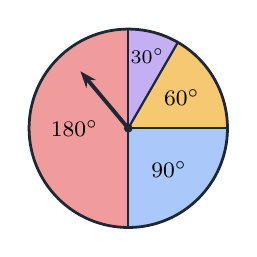
\begin{tikzpicture}[scale=1.05]
\fill[AnsRed!45] (0,0)--(90:1.2) arc (90:270:1.2)--cycle;
\fill[tmBlue!45] (0,0)--(270:1.2) arc (270:360:1.2)--cycle;
\fill[StarGold!70] (0,0)--(0:1.2) arc (0:60:1.2)--cycle;
\fill[tmPurple!45] (0,0)--(60:1.2) arc (60:90:1.2)--cycle;
\draw[Ink,line width=1pt] (0,0) circle (1.2);
\foreach \a in {90,270,0,60}{\draw[Ink,line width=0.8pt] (0,0)--(\a:1.2);}
\node[font=\footnotesize] at (180:0.65){$180^\circ$};
\node[font=\footnotesize] at (315:0.7){$90^\circ$};
\node[font=\footnotesize] at (30:0.75){$60^\circ$};
\node[font=\scriptsize] at (75:0.9){$30^\circ$};
\draw[-{Stealth[length=6pt]},line width=1.4pt,Ink] (0,0)--(130:0.9);\fill[Ink] (0,0) circle (1.5pt);
\end{tikzpicture}
\end{minipage}
\end{probbox}
\probsol{
\textbf{Understanding the problem.} The sectors have \emph{different} sizes, so the four sectors are \emph{not} equally likely. We cannot use ``$1$ sector out of $4$''. Instead, the chance of the arrow stopping in a sector is proportional to the size of the sector, that is, to its central angle.
\begin{recallbox}For a spinner with unequal sectors: $P(\text{sector})=\dfrac{\text{central angle of the sector}}{360^\circ}$. The whole circle has $360^\circ$.\end{recallbox}
\step{1}{Check the data}
$180^\circ+90^\circ+60^\circ+30^\circ=360^\circ$ -- exactly one full circle \checkmark.
\step{2}{Part a}
$P(\text{blue})=\dfrac{90}{360}=\dfrac14$.

\emph{Another way to think:} we can divide the spinner into $12$ equal small sectors of $30^\circ$ each. Then red takes $6$ small sectors, blue $3$, yellow $2$ and purple $1$; these $12$ small sectors are equally likely. $P(\text{blue})=\dfrac{3}{12}=\dfrac14$ \checkmark.
\step{3}{Part b}
The yellow and purple sectors do not overlap, so their total angle is $60^\circ+30^\circ=90^\circ$.
$P(\text{yellow or purple})=\dfrac{90}{360}=\dfrac14$ (or $\dfrac{2+1}{12}=\dfrac{3}{12}=\dfrac14$).
\step{4}{Part c}
Hùng is \textbf{wrong}. The formula ``favourable divided by all'' only works when the outcomes are \emph{equally likely}. Here the four colours are not equally likely: the red sector is half of the spinner, so $P(\text{red})=\dfrac{180}{360}=\dfrac12$, while $P(\text{purple})=\dfrac{30}{360}=\dfrac{1}{12}$ -- very different.
\verify{$P(\text{red})+P(\text{blue})+P(\text{yellow})+P(\text{purple})=\dfrac{6}{12}+\dfrac{3}{12}+\dfrac{2}{12}+\dfrac{1}{12}=1$ \checkmark.}
\begin{parentbox}Cut a paper plate into $12$ equal ``slices of cake'' and colour them as in the problem. Counting the slices of each colour, your child will see at once why a big sector has a big probability.\end{parentbox}
\ans{a) $\dfrac14$;\quad b) $\dfrac14$;\quad c) Wrong, because the sectors are not equal (e.g.\ $P(\text{red})=\dfrac12$, $P(\text{purple})=\dfrac1{12}$).}
}

% ---------------------------------------------------------------- Problem 33
\begin{probbox}{33}{\relax}
The school canteen has this lunch menu: one main dish out of $3$ (chicken rice, phở, bún chả); one drink out of $2$ (iced tea, orange juice); one dessert out of $2$ (chè, yoghurt). Each lunch consists of one main dish, one drink and one dessert.
\begin{enumerate}[label=\alph*),leftmargin=1.5em,itemsep=0pt,topsep=2pt]
\item How many different lunches are there?
\item Lan is given a lunch at random. Find the probability that it includes phở.
\item Find the probability that Lan's lunch includes both phở and orange juice.
\end{enumerate}
\end{probbox}
\probsol{
\textbf{Understanding the problem.} Each lunch is made by three successive choices: main dish, drink, dessert. ``Given at random'' means all the different lunches are equally likely.
\step{1}{Part a -- multiplication rule}
\begin{recallbox}Multiplication rule: if a task has stages with $m$, $n$ and $p$ ways, there are $m\times n\times p$ ways altogether.\end{recallbox}
Number of lunches: $3\times2\times2=12$.
\begin{center}\begin{tikzpicture}[grow'=right,level distance=2.6cm,font=\sffamily\footnotesize,
  every node/.style={draw=tmBlue,fill=tmBlue!8,rounded corners=2pt,inner sep=2pt},
  level 1/.style={sibling distance=2.4cm},level 2/.style={sibling distance=1.2cm},level 3/.style={sibling distance=0.6cm},
  edge from parent/.style={draw=Ink!60}]
\node[fill=Ink!10,draw=Ink]{Lunch}
  child{node{chicken rice} child{node{iced tea} child{node{chè}} child{node{yoghurt}}} child{node{orange juice} child{node{chè}} child{node{yoghurt}}}}
  child{node[fill=tmOrange!25,draw=tmOrange]{phở} child{node{iced tea} child{node{chè}} child{node{yoghurt}}} child{node[fill=tmOrange!25,draw=tmOrange]{orange juice} child{node[fill=tmOrange!25,draw=tmOrange]{chè}} child{node[fill=tmOrange!25,draw=tmOrange]{yoghurt}}}}
  child{node{bún chả} child{node{iced tea} child{node{chè}} child{node{yoghurt}}} child{node{orange juice} child{node{chè}} child{node{yoghurt}}}};
\end{tikzpicture}\end{center}
The tree has $3$ big branches, each splitting into $2$ branches, each of which splits into $2$ again: $12$ end points, exactly $12$ lunches.
\step{2}{Part b}
Lunches with phở: the main dish is fixed as phở, drink $2$ ways, dessert $2$ ways: $1\times2\times2=4$ lunches (the middle branch of the tree).
$P(\text{phở})=\dfrac{4}{12}=\dfrac13$.
\begin{tipbox}A quick way to think: the main dish is chosen at random from $3$ dishes, and each dish appears in the same number of lunches, so $P(\text{phở})=\dfrac13$. The drink and dessert do not matter.\end{tipbox}
\step{3}{Part c}
Main dish phở, drink orange juice, only the dessert is left to choose: $1\times1\times2=2$ lunches (orange in the tree).
$P(\text{phở and orange juice})=\dfrac{2}{12}=\dfrac16$.
\verify{List them: (phở, orange juice, chè) and (phở, orange juice, yoghurt) -- exactly $2$ lunches \checkmark.}
\ans{a) $12$ lunches;\quad b) $\dfrac13$;\quad c) $\dfrac16$.}
}

% ---------------------------------------------------------------- Problem 34
\begin{probbox}{34}{\relax}
A hall has $20$ rows of seats. The first row has $12$ seats, and each row behind has $2$ seats more than the row just in front of it.
\begin{enumerate}[label=\alph*),leftmargin=1.5em,itemsep=0pt,topsep=2pt]
\item How many seats are in row $20$?
\item Which row has exactly $30$ seats?
\item How many seats does the hall have altogether?
\end{enumerate}
\end{probbox}
\probsol{
\textbf{Understanding the problem.} The numbers of seats in the rows are $12,14,16,\dots$ -- an \emph{evenly spaced sequence} with step $d=2$. We need the $20$th term, the position of the term $30$, and the sum of $20$ terms.
\step{1}{Part a -- find the pattern}
\begin{center}
\begin{tabular}{|c|c|c|c|c|c|}\hline
Row & $1$ & $2$ & $3$ & $4$ & $k$\\ \hline
Seats & $12$ & $12+2$ & $12+2\times2$ & $12+3\times2$ & $12+(k-1)\times2$\\ \hline
\end{tabular}
\end{center}
From row $1$ to row $k$ there are $k-1$ ``jumps'', each adding $2$ seats. Row $20$: $12+19\times2=12+38=50$ seats.
\begin{warnbox}Not $12+20\times2=52$: from row $1$ to row $20$ there are only $19$ increases (the ``off by one'' error).\end{warnbox}
\step{2}{Part b}
We need $12+(k-1)\times2=30$, so $(k-1)\times2=18$, $k-1=9$, $k=10$. Row $10$ has $30$ seats.
\step{3}{Part c -- sum of an evenly spaced sequence}
\begin{recallbox}Sum of an evenly spaced sequence $=\dfrac{(\text{first}+\text{last})\times\text{number of terms}}{2}$ (Gauss's pairing method).\end{recallbox}
Total number of seats: $\dfrac{(12+50)\times20}{2}=\dfrac{62\times20}{2}=620$ seats.
\begin{proofbox}Pair row $1$ with row $20$: $12+50=62$; row $2$ with row $19$: $14+48=62$; \ldots; row $10$ with row $11$: $30+32=62$. There are $10$ pairs of $62$ seats each, so the total is $10\times62=620$.\end{proofbox}
\verify{Another way: if every row had $12$ seats there would be $20\times12=240$ seats; the ``extra'' is $0+2+4+\dots+38=2\times(0+1+\dots+19)=2\times190=380$; total $240+380=620$ \checkmark.}
\ans{a) $50$ seats;\quad b) row $10$;\quad c) $620$ seats.}
}

% ---------------------------------------------------------------- Problem 35
\begin{probbox}{35}{\stars{1}}
A box contains only red and blue marbles. If one marble is drawn at random, the probability that it is red is $\dfrac35$. If $5$ more blue marbles are put into the box, the probability of drawing a red marble drops to $\dfrac12$. How many red marbles and how many blue marbles were in the box at the start?
\end{probbox}
\probsol{
\textbf{Understanding the problem.} We do not know the total number of marbles, only \emph{proportions}. Adding blue marbles does not change the number of red marbles. Let us translate the two probabilities into the language of ``equal parts'' (a bar model).
\step{1}{Translate the first condition}
$P(\text{red})=\dfrac35$: if the marbles are split into $5$ equal parts, red takes $3$ parts and blue takes $5-3=2$ parts.
\step{2}{Translate the second condition}
After adding $5$ blue marbles, $P(\text{red})=\dfrac12$: red makes up exactly half, i.e.\ \emph{the number of red marbles equals the number of blue marbles}.
\step{3}{Draw the model and compare}
\begin{figC}
\rowlab{-0.15}{0}{Red}
\blk{0}{1.5}{0}{0.55}{AnsRed}{1 part}\blk{1.5}{3}{0}{0.55}{AnsRed}{1 part}\blk{3}{4.5}{0}{0.55}{AnsRed}{1 part}
\rowlab{-0.15}{-0.8}{Blue}
\blk{0}{1.5}{-0.8}{0.55}{tmBlue}{1 part}\blk{1.5}{3}{-0.8}{0.55}{tmBlue}{1 part}\blk{3}{4.5}{-0.8}{0.55}{tmTeal}{add 5}
\brcdn{3}{4.5}{-1.25}{$1$ part $=5$ marbles}
\end{figC}
Red: $3$ parts. Blue after adding: $2$ parts $+\ 5$ marbles. These are equal, so the $5$ marbles are exactly $3-2=1$ part.
\step{4}{Compute the numbers at the start}
$1$ part $=5$ marbles. Red: $3\times5=15$ marbles. Blue: $2\times5=10$ marbles.
\begin{tipbox}\emph{Algebra version (for those who like it):} let the number of red marbles be $3k$ and blue $2k$. After adding: $3k=2k+5$, so $k=5$.\end{tipbox}
\verify{At the start: $15$ red, $10$ blue, $P(\text{red})=\dfrac{15}{25}=\dfrac35$ \checkmark. Adding $5$ blue: $15$ red, $15$ blue, $P(\text{red})=\dfrac{15}{30}=\dfrac12$ \checkmark.}
\begin{warnbox}Do not try to ``subtract probabilities'': $\dfrac35-\dfrac12=\dfrac1{10}$ tells us nothing directly about the number of marbles. A probability is a \emph{ratio}; go back to actual quantities.\end{warnbox}
\ans{At the start there were $15$ red and $10$ blue marbles.}
}

% ---------------------------------------------------------------- Problem 36
\begin{probbox}{36}{\stars{1}}
Recall: a palindrome is a number that reads the same forwards and backwards (for example $3443$, $7007$).
\begin{enumerate}[label=\alph*),leftmargin=1.5em,itemsep=0pt,topsep=2pt]
\item How many four-digit palindromes are there?
\item How many of them are even?
\item A four-digit palindrome is chosen at random. Find the probability that it is even.
\item Show that every four-digit palindrome is divisible by $11$.
\end{enumerate}
\end{probbox}
\probsol{
\textbf{Understanding the problem.} A four-digit number $\overline{abcd}$ is a palindrome when reading it backwards, $\overline{dcba}$, gives the same number: $d=a$ and $c=b$. So a four-digit palindrome has the form $\overline{abba}$, and only \emph{two} digits are chosen freely: $a$ and $b$.
\step{1}{Part a}
\begin{recallbox}Multiplication rule; the first digit of a number cannot be $0$.\end{recallbox}
\countboxes{digit a/9/from 1 to 9/tmBlue,digit b/10/from 0 to 9/tmOrange,third/1/equals b/tmGreen,fourth/1/equals a/tmGreen}{90}
$a$: $9$ ways ($1$ to $9$); $b$: $10$ ways; the last two digits are forced to equal $b$ and $a$. There are $9\times10=90$ numbers.
\step{2}{Part b}
A number is even when its ones digit is even. The ones digit is $a$, so $a$ must be even \emph{and} non-zero: $a\in\{2,4,6,8\}$ -- $4$ ways. $b$ still has $10$ ways. There are $4\times10=40$ even palindromes.
\begin{warnbox}The digit $0$ is even, but $a=0$ is not allowed because $a$ is also the first digit. So there are $4$, not $5$, choices for $a$.\end{warnbox}
\step{3}{Part c}
$P(\text{even})=\dfrac{40}{90}=\dfrac49$.
\step{4}{Part d -- proof}
\begin{proofbox}Write $\overline{abba}$ using place values:
$\overline{abba}=1000a+100b+10b+a=1001a+110b$.
Since $1001=11\times91$ and $110=11\times10$,
$\overline{abba}=11\times91\times a+11\times10\times b=11\times(91a+10b)$,
which is divisible by $11$.\end{proofbox}
\verify{Examples: $3443=11\times313$; $7007=11\times637$; $1221=11\times111$ \checkmark. Counting check: the palindromes starting with $1$ are $1001,1111,\dots,1991$ -- exactly $10$ numbers; nine first digits give $90$ numbers \checkmark.}
\ans{a) $90$;\quad b) $40$;\quad c) $\dfrac49$;\quad d) $\overline{abba}=11\times(91a+10b)$.}
}

% ---------------------------------------------------------------- Problem 37
\begin{probbox}{37}{\stars{1}}
Using the four digits $0,1,2,3$, four-digit numbers with all digits different are made (each digit used exactly once).
\begin{enumerate}[label=\alph*),leftmargin=1.5em,itemsep=0pt,topsep=2pt]
\item How many such numbers can be made?
\item How many of them are even?
\item One of the numbers from part a) is chosen at random. Find the probability that it is even.
\end{enumerate}
\end{probbox}
\probsol{
\textbf{Understanding the problem.} Each number is an arrangement of the four digits $0,1,2,3$ in the four places (thousands, hundreds, tens, ones), with the condition that the thousands digit is not $0$.
\step{1}{Part a -- choose the restricted position first}
\begin{recallbox}Multiplication rule. A position with a condition is chosen first.\end{recallbox}
\countboxes{thousands/3/1 2 or 3/tmBlue,hundreds/3/0 allowed/tmOrange,tens/2/remaining/tmGreen,ones/1/remaining/tmPurple}{18}
Thousands: $3$ ways ($1$, $2$ or $3$). Hundreds: $3$ digits left (now $0$ may be used): $3$ ways. Tens: $2$ ways. Ones: $1$ way. There are $3\times3\times2\times1=18$ numbers.
\begin{warnbox}Forgetting the condition ``thousands digit not $0$'' gives $4\times3\times2\times1=24$ -- which includes $6$ ``numbers'' starting with $0$, such as $0123$, that are really three-digit numbers.\end{warnbox}
\step{2}{Part b -- split into cases by the ones digit}
An even number ends in $0$ or $2$. These two cases differ because the digit $0$ affects the thousands place.
\begin{itemize}[leftmargin=1.2em,itemsep=1pt,topsep=1pt]
\item \textbf{Case 1: ones digit $0$.} The three digits $1,2,3$ go freely into the other three places (no more worry about $0$ in front): $3\times2\times1=6$ numbers.
\item \textbf{Case 2: ones digit $2$.} $0,1,3$ remain. Thousands not $0$: $2$ ways ($1$ or $3$); hundreds: $2$ ways; tens: $1$ way. There are $2\times2\times1=4$ numbers.
\end{itemize}
\begin{recallbox}Addition rule: for separate cases, add the numbers of ways in each case.\end{recallbox}
Number of even numbers: $6+4=10$.
\step{3}{Part c}
$P(\text{even})=\dfrac{10}{18}=\dfrac59$.
\verify{List the even numbers. Case 1: $1230,1320,2130,2310,3120,3210$ ($6$ numbers). Case 2: $1032,1302,3012,3102$ ($4$ numbers). Total $10$ \checkmark. Odd numbers (ending in $1$ or $3$): each case is like Case 2, with $4$ numbers, total $8$; and $10+8=18$ \checkmark.}
\ans{a) $18$ numbers;\quad b) $10$ even numbers;\quad c) $\dfrac59$.}
}

% ---------------------------------------------------------------- Problem 38
\begin{probbox}{38}{\stars{1}}
\begin{minipage}[t]{0.62\linewidth}\vspace{0pt}
The figure shows a rectangular grid of $2$ rows and $3$ columns of squares.
\begin{enumerate}[label=\alph*),leftmargin=1.5em,itemsep=0pt,topsep=2pt]
\item How many rectangles (including squares) are there in the figure altogether?
\item How many squares are there?
\item One of these rectangles is chosen at random. Find the probability that it is a square.
\end{enumerate}
\end{minipage}\hfill
\begin{minipage}[t]{0.34\linewidth}\vspace{0pt}
\centering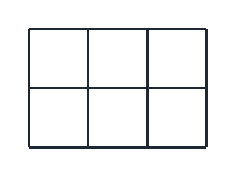
\begin{tikzpicture}[scale=0.75]
\foreach \x in {0,1,2,3}{\draw[Ink,line width=1pt] (\x,0)--(\x,2);}
\foreach \y in {0,1,2}{\draw[Ink,line width=1pt] (0,\y)--(3,\y);}
\end{tikzpicture}
\end{minipage}
\end{probbox}
\probsol{
\textbf{Understanding the problem.} This is a grid with full-length lines, so the ``choose two lines'' trick works. We will also count by size to check.
\step{1}{Part a -- choose two horizontal and two vertical lines}
\begin{recallbox}A rectangle in a grid is determined by $2$ horizontal and $2$ vertical lines. The number of ways to choose $2$ of $n$ lines is $\dfrac{n\times(n-1)}{2}$.\end{recallbox}
The grid has $3$ horizontal and $4$ vertical lines.
\begin{itemize}[leftmargin=1.2em,itemsep=0pt,topsep=1pt]
\item Choose $2$ horizontal lines: $\dfrac{3\times2}{2}=3$ ways.
\item Choose $2$ vertical lines: $\dfrac{4\times3}{2}=6$ ways.
\end{itemize}
By the multiplication rule: $3\times6=18$ rectangles.
\step{2}{Check with a table of sizes}
Write ``height $\times$ width'' (in squares). A shape $w$ squares wide has $4-w$ horizontal positions; $h$ squares high, $3-h$ vertical positions.
\begin{center}
\begin{tabular}{|c|c|c|c|c|c|c|c|}\hline
Size & $1\times1$ & $1\times2$ & $1\times3$ & $2\times1$ & $2\times2$ & $2\times3$ & Total\\ \hline
Number & $2\times3=6$ & $2\times2=4$ & $2\times1=2$ & $1\times3=3$ & $1\times2=2$ & $1\times1=1$ & $18$\\ \hline
\end{tabular}
\end{center}
Both methods give $18$ \checkmark.
\step{3}{Part b}
The squares are the $1\times1$ and $2\times2$ shapes: $6+2=8$ squares.
\begin{warnbox}There is no $3\times3$ square because the grid is only $2$ squares high. And do not forget the two $2\times2$ squares (left and right, overlapping in the middle column).\end{warnbox}
\step{4}{Part c}
$P(\text{square})=\dfrac{8}{18}=\dfrac49$.
\ans{a) $18$;\quad b) $8$;\quad c) $\dfrac49$.}
}

% ---------------------------------------------------------------- Problem 39
\begin{probbox}{39}{\stars{1}}
Four friends An, Bình, Chi and Dũng are seated at random on four chairs in a row.
\begin{enumerate}[label=\alph*),leftmargin=1.5em,itemsep=0pt,topsep=2pt]
\item How many seating arrangements are there?
\item Find the probability that An and Bình sit next to each other.
\item Find the probability that An and Bình sit at the two ends of the row.
\end{enumerate}
\end{probbox}
\probsol{
\textbf{Understanding the problem.} ``Seated at random'' means all arrangements are equally likely. We count all arrangements, then the favourable ones for each event. Number the chairs $1,2,3,4$ from left to right.
\step{1}{Part a}
\begin{recallbox}Seating $n$ people on $n$ chairs: $n\times(n-1)\times\dots\times2\times1$ ways (multiplication rule; each next chair has one person fewer to choose from).\end{recallbox}
Chair $1$: $4$ choices of person; chair $2$: $3$; chair $3$: $2$; chair $4$: $1$. There are $4\times3\times2\times1=24$ arrangements.
\step{2}{Part b -- treat An and Bình as one ``block''}
\begin{figC}
\draw[tmOrange,line width=1.2pt,rounded corners=4pt,fill=tmOrange!12] (0,0) rectangle (2.4,0.7);
\node[font=\bfseries] at (0.6,0.35){An};\node[font=\bfseries] at (1.8,0.35){Bình};
\draw[tmBlue,line width=1pt,rounded corners=3pt,fill=tmBlue!10] (2.7,0) rectangle (3.9,0.7);\node[font=\bfseries] at (3.3,0.35){Chi};
\draw[tmGreen,line width=1pt,rounded corners=3pt,fill=tmGreen!10] (4.2,0) rectangle (5.4,0.7);\node[font=\bfseries] at (4.8,0.35){Dũng};
\node[font=\footnotesize,text=tmOrange!80!black] at (1.2,-0.3){one block, taking $2$ neighbouring chairs};
\end{figC}
\begin{itemize}[leftmargin=1.2em,itemsep=1pt,topsep=1pt]
\item Position of the block (An, Bình): chairs $1$--$2$, $2$--$3$ or $3$--$4$: $3$ ways.
\item Inside the block, An on the left or Bình on the left: $2$ ways.
\item Chi and Dũng on the $2$ remaining chairs: $2\times1=2$ ways.
\end{itemize}
Favourable arrangements: $3\times2\times2=12$. So $P(\text{next to each other})=\dfrac{12}{24}=\dfrac12$.
\begin{warnbox}Do not forget to multiply by $2$ for swapping An and Bình inside the block: ``An--Bình'' and ``Bình--An'' are two different arrangements.\end{warnbox}
\step{3}{Part c}
An and Bình on chairs $1$ and $4$: An on chair $1$ and Bình on chair $4$, or the other way round -- $2$ ways. Chi and Dũng on chairs $2$, $3$: $2$ ways. Favourable arrangements: $2\times2=4$.
$P(\text{both ends})=\dfrac{4}{24}=\dfrac16$.
\verify{Part b, counted another way: if An sits at an end (chair $1$ or $4$, $2$ possibilities) there is only $1$ chair next to An; if An sits in the middle (chair $2$ or $3$) there are $2$ chairs next to An. Number of (An, Bình) neighbouring chair pairs: $2\times1+2\times2=6$; times $2$ ways to seat Chi and Dũng: $12$ \checkmark.}
\begin{parentbox}With $4$ people, let your child use $4$ name cards and actually lay out all $24$ arrangements in order (starting with An, then starting with Bình\ldots). Listing once helps the child trust the multiplication rule.\end{parentbox}
\ans{a) $24$ arrangements;\quad b) $\dfrac12$;\quad c) $\dfrac16$.}
}

% ---------------------------------------------------------------- Problem 40
\begin{probbox}{40}{\stars{2}}
A box contains $4$ red marbles and $6$ blue marbles of the same size. Hoa draws one marble at random, does \emph{not put it back}, and then draws a second marble at random.
\begin{enumerate}[label=\alph*),leftmargin=1.5em,itemsep=0pt,topsep=2pt]
\item Find the probability that both marbles are red.
\item Find the probability that the two marbles have the same colour.
\item Find the probability that the two marbles have different colours.
\end{enumerate}
\end{probbox}
\probsol{
\textbf{Understanding the problem.} Hoa draws two marbles \emph{one after the other} without replacement. Imagine the marbles numbered $1$ to $10$ (marbles $1$--$4$ red, marbles $5$--$10$ blue). Each \emph{ordered pair} (first marble, second marble) is one outcome, and these outcomes are equally likely.
\step{1}{Count all outcomes}
\begin{recallbox}Multiplication rule: the first draw has $10$ ways; for each of them, the second draw has $9$ marbles left, so $9$ ways.\end{recallbox}
Number of outcomes: $10\times9=90$ ordered pairs.
\step{2}{Part a -- both red}
First draw red: $4$ ways. Then $3$ red marbles are left, second draw red: $3$ ways. Favourable outcomes: $4\times3=12$.
$P(\text{red, red})=\dfrac{12}{90}=\dfrac{2}{15}$.
\step{3}{Tree diagram with the numbers of ways}
\begin{center}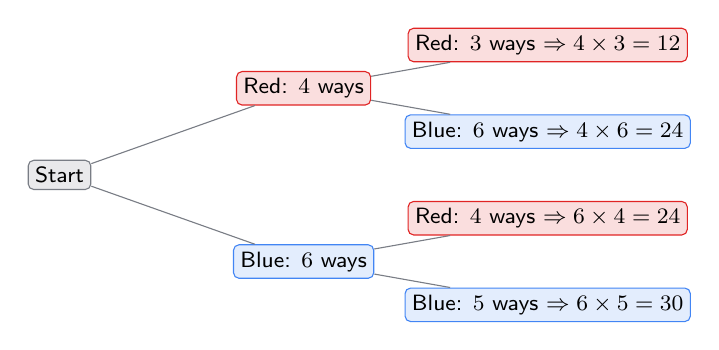
\begin{tikzpicture}[grow'=right,level distance=3.1cm,font=\sffamily\footnotesize,
  every node/.style={draw=Ink!60,rounded corners=2pt,inner sep=2.5pt,fill=white},
  level 1/.style={sibling distance=2.2cm},level 2/.style={sibling distance=1.1cm},
  edge from parent/.style={draw=Ink!60}]
\node[fill=Ink!10]{Start}
  child{node[fill=AnsRed!15,draw=AnsRed]{Red: $4$ ways}
     child{node[fill=AnsRed!15,draw=AnsRed]{Red: $3$ ways $\Rightarrow 4\times3=12$}}
     child{node[fill=tmBlue!15,draw=tmBlue]{Blue: $6$ ways $\Rightarrow 4\times6=24$}}}
  child{node[fill=tmBlue!15,draw=tmBlue]{Blue: $6$ ways}
     child{node[fill=AnsRed!15,draw=AnsRed]{Red: $4$ ways $\Rightarrow 6\times4=24$}}
     child{node[fill=tmBlue!15,draw=tmBlue]{Blue: $5$ ways $\Rightarrow 6\times5=30$}}};
\end{tikzpicture}\end{center}
Check: $12+24+24+30=90$ \checkmark{} -- the four branches cover every outcome.
\step{4}{Part b -- same colour}
Same colour has two separate cases: (red, red) with $12$ outcomes and (blue, blue) with $30$ outcomes.
\begin{recallbox}Addition rule for cases that do not overlap.\end{recallbox}
Favourable outcomes: $12+30=42$. $P(\text{same colour})=\dfrac{42}{90}=\dfrac{7}{15}$.
\step{5}{Part c -- complement}
``Different colours'' is the complement of ``same colour'': $P(\text{different colours})=1-\dfrac{7}{15}=\dfrac{8}{15}$.
\verify{Direct count: (red, blue) $24$ and (blue, red) $24$, total $48$; $\dfrac{48}{90}=\dfrac{8}{15}$ \checkmark.}
\begin{warnbox}The most common mistake: acting as if all $10$ marbles are still there for the second draw, computing $\dfrac{4}{10}\times\dfrac{4}{10}$ or counting $4\times4$ red pairs. Because the marble is \emph{not put back}, the second draw has only $9$ marbles and only $3$ red ones.\end{warnbox}
\begin{tipbox}You can also count without order: the number of ways to choose $2$ of $10$ marbles is $\dfrac{10\times9}{2}=45$, the number of ways to choose $2$ of the $4$ red marbles is $\dfrac{4\times3}{2}=6$, so $P(\text{red, red})=\dfrac{6}{45}=\dfrac{2}{15}$ -- the same result. What matters is that the numerator and denominator are counted \emph{the same way} (both ordered or both unordered).\end{tipbox}
\ans{a) $\dfrac{2}{15}$;\quad b) $\dfrac{7}{15}$;\quad c) $\dfrac{8}{15}$.}
}

% ---------------- part d ----------------
% ================= Topic 3 (EN) -- part d: problems 41--50 (challenge) =================
\begin{probbox}{41}{\stars{1}}
On a square dot grid, Lan stands at dot $A$. She tosses a fair coin $6$ times; each time it shows heads she moves \emph{up} one dot, and
each time it shows tails she moves \emph{right} one dot (as in problem 16). The dots $M$, $N$, $B$ are marked in the figure.
\begin{figC}\begin{scope}[scale=0.85]
  \foreach \x in {0,...,3}{\foreach \y in {0,...,3}{\fill[Navy] (\x,\y) circle (2.4pt);}}
  \fill[tmOrange] (0,0) circle (3.4pt);\node[below left] at (0,0) {$A$};
  \fill[tmGreen!80!black] (1,1) circle (3.4pt);\node[above left] at (1,1) {$M$};
  \fill[AnsRed] (2,1) circle (3.4pt);\node[below right] at (2,1) {$N$};
  \fill[tmPurple] (3,3) circle (3.4pt);\node[above right] at (3,3) {$B$};
\end{scope}\end{figC}
\begin{enumerate}[label=\alph*),leftmargin=1.6em,itemsep=1pt,topsep=2pt]
\item Find the probability that after $6$ tosses Lan stops at dot $B$.
\item Find the probability that Lan passes through dot $M$ \emph{and} stops at $B$.
\item Find the probability that Lan stops at $B$ \emph{without} passing through dot $N$.
\end{enumerate}
\end{probbox}
\probsol{
\textbf{Understanding the problem.} Each sequence of $6$ tosses is a sequence of $6$ symbols $\uparrow$ (up) or $\rightarrow$ (right).
There are $2^6=2\times2\times2\times2\times2\times2=64$ sequences, all equally likely. Each sequence is a \emph{path} on the grid.
We label positions by the pair (number of moves right, number of moves up): $A=(0,0)$, $M=(1,1)$, $N=(2,1)$, $B=(3,3)$.

\step{1}{Count the paths from $A$ to every dot (part a)}
\begin{recallbox}A dot can only be reached from the dot just to its left or the dot just below it. Therefore:
number of paths to a dot $=$ number of paths to the dot on its left $+$ number of paths to the dot below (addition principle).\end{recallbox}
Write the number of paths at each dot, starting from $A$ (write $1$); the bottom row and the left column are all $1$:
\begin{figC}\begin{scope}[scale=0.85]
  \foreach \x/\y/\n in {0/0/1,1/0/1,2/0/1,3/0/1,0/1/1,1/1/2,2/1/3,3/1/4,0/2/1,1/2/3,2/2/6,3/2/10,0/3/1,1/3/4,2/3/10,3/3/20}{
    \fill[tmBlue!12] (\x,\y) circle (9pt);\node[font=\small\bfseries,text=Navy] at (\x,\y) {\n};}
  \draw[tmPurple,thick] (3,3) circle (10pt);\node[right=9pt,text=tmPurple] at (3,3) {$B$};
\end{scope}\end{figC}
There are $20$ paths from $A$ to $B$. (Another way: reaching $B$ needs exactly $3$ up-moves among the $6$ moves; the number of ways to
choose $3$ turns out of $6$ is $\dfrac{6\times5\times4}{3\times2\times1}=20$.)
\[P(a)=\frac{20}{64}=\frac{5}{16}.\]

\step{2}{Part b: through $M$ and then to $B$ -- multiplication principle}
A path through $M$ has two stages: stage $A\to M$ ($1$ up, $1$ right) and stage $M\to B$ ($2$ up, $2$ right).
Stage $A\to M$ can be done in $2$ ways ($\uparrow\rightarrow$ or $\rightarrow\uparrow$); stage $M\to B$ in $6$ ways (as in problem 16:
choose $2$ up-turns out of $4$). Each way of doing the first stage combined with each way of doing the second gives a different path:
$2\times6=12$ paths.
\[P(b)=\frac{12}{64}=\frac{3}{16}.\]

\step{3}{Part c: avoiding $N$ -- use the complement}
Paths from $A$ through $N$ to $B$: stage $A\to N$ ($2$ right, $1$ up) has $3$ ways; stage $N\to B$ ($1$ right, $2$ up) has $3$ ways;
in total $3\times3=9$ paths. So the number of paths from $A$ to $B$ \emph{not} through $N$ is $20-9=11$.
\[P(c)=\frac{11}{64}.\]
\begin{proofbox}\emph{Check by ``blocking'' dot $N$.} Recompute the path numbers but put $0$ at $N$ (as if it cannot be used).
Row $1$: $1,\ 2,\ \mathbf{0},\ 0+1=1$. Row $2$: $1,\ 3,\ 3+0=3,\ 3+1=4$. Row $3$: $1,\ 4,\ 4+3=7,\ 7+4=11$.
At $B$ we get $11$, matching the complement.\end{proofbox}
\begin{warnbox}Parts b and c ask for probabilities among \emph{all} $64$ toss sequences, not among the $20$ paths to $B$. Dividing by $20$
answers a different question (a conditional probability, not yet studied).\end{warnbox}
\verify{In part a the possible final dots are $(6,0),(5,1),\dots,(0,6)$ with $1,6,15,20,15,6,1$ paths; the total is $64$. Dot $B=(3,3)$
corresponds to $20$.}
\ans{a) $\dfrac5{16}$;\quad b) $\dfrac3{16}$;\quad c) $\dfrac{11}{64}$}
}

\begin{probbox}{42}{\stars{2}}
We build grids of squares from toothpicks as in problem 17. An ``$m\times n$'' grid has $m$ rows, each with $n$ squares.
\begin{enumerate}[label=\alph*),leftmargin=1.6em,itemsep=1pt,topsep=2pt]
\item Find a formula for the number of toothpicks needed for an $m\times n$ grid.
\item A square $k\times k$ grid uses exactly $760$ toothpicks. Find $k$.
\item Nam has exactly $2026$ toothpicks and wants to build an $m\times n$ grid (with $1\le m\le n$) that uses \emph{all} of them.
Find all the grids Nam can build.
\end{enumerate}
\end{probbox}
\probsol{
\textbf{Understanding the problem.} As in problem 17, we count horizontal and vertical toothpicks separately. Part c leads to an equation in
two natural-number unknowns; the trick ``multiply by $2$ and add $1$'' turns it into a problem about divisors.

\step{1}{Part a: the formula}
An $m\times n$ grid has $m+1$ horizontal lines of $n$ toothpicks each: $(m+1)\times n$ horizontal toothpicks. It has $n+1$ vertical lines of
$m$ toothpicks each: $(n+1)\times m$ vertical toothpicks. Total:
\[T=(m+1)n+(n+1)m=mn+n+mn+m=2mn+m+n.\]
Check with the $1\times10$ grid: $2\times1\times10+1+10=31$, as in problem 17.

\step{2}{Part b: a square $k\times k$ grid}
Put $m=n=k$: $T=2k^2+2k=2k(k+1)$. We need $2k(k+1)=760$, that is $k(k+1)=380$.
$k(k+1)$ is the product of two consecutive natural numbers. Since $19\times20=380$, $k=19$. (As $k$ grows, $k(k+1)$ grows, so there is only
one value: $18\times19=342<380<420=20\times21$.)

\step{3}{Part c: set up the equation}
We need natural numbers $1\le m\le n$ with $2mn+m+n=2026$.
\begin{tipbox}Multiply both sides by $2$ and add $1$: $4mn+2m+2n+1=4053$. The left side factorises:
$(2m+1)(2n+1)=4mn+2m+2n+1$ (expand to check). So
\[(2m+1)(2n+1)=4053.\]\end{tipbox}

\step{4}{Prime factorisation of $4053$}
The digit sum of $4053$ is $4+0+5+3=12$, divisible by $3$: $4053=3\times1351$. Next, $1351=7\times193$.
The number $193$ is prime: it is not divisible by $2,3,5,7,11,13$, and $13\times13=169<193<196=14\times14$, so no more trials are needed.
\begin{recallbox}To check whether $N$ is prime, it is enough to try dividing by the primes $p$ with $p\times p\le N$.\end{recallbox}
So $4053=3\times7\times193$. The divisors of $4053$ are: $1,\ 3,\ 7,\ 21,\ 193,\ 579,\ 1351,\ 4053$.

\step{5}{Find the pairs $(m,n)$}
Since $m\ge1$, $2m+1\ge3$; since $m\le n$, $2m+1\le2n+1$. The ways of writing $4053$ as a product of two such divisors:
\begin{center}\begin{tabular}{|c|c|c|c|c|}\hline
$2m+1$ & $2n+1$ & $m$ & $n$ & Check $2mn+m+n$\\\hline
$3$ & $1351$ & $1$ & $675$ & $1350+1+675=2026$\\\hline
$7$ & $579$ & $3$ & $289$ & $1734+3+289=2026$\\\hline
$21$ & $193$ & $10$ & $96$ & $1920+10+96=2026$\\\hline
\end{tabular}\end{center}
(The pair $1\times4053$ is rejected because it gives $m=0$.)
\begin{warnbox}Trying $m=1,2,3,\dots$ one by one also works but is very long and it is easy to miss a solution. The ``multiply by $2$, add $1$''
trick turns the problem into ``find the divisors'' and guarantees that \emph{no} solution is missed.\end{warnbox}
\verify{For any other value of $m$, $2m+1$ is not a divisor of $4053$, so $n$ is not a natural number. For example $m=2$: $5(2n+1)=4053$ is
impossible because $4053$ is not divisible by $5$.}
\ans{a) $2mn+m+n$;\quad b) $k=19$;\quad c) three grids: $1\times675$, $3\times289$, $10\times96$}
}

\begin{probbox}{43}{\stars{1}}
Three fair dice coloured red, blue and yellow are rolled together (each is numbered $1$ to $6$). Find the probability of each event:
\begin{enumerate}[label=\alph*),leftmargin=1.6em,itemsep=1pt,topsep=2pt]
\item the three numbers are all different;
\item the number on the red die is less than the number on the blue die, and the number on the blue die is less than the number on the
yellow die;
\item at least one die shows a $6$;
\item the largest of the three numbers is exactly $4$.
\end{enumerate}
\end{probbox}
\probsol{
\textbf{Understanding the problem.} Each outcome is a triple (red, blue, yellow). By the multiplication principle there are
$6\times6\times6=216$ equally likely outcomes.

\step{1}{Part a: three different numbers}
Red die: $6$ ways; blue die different from red: $5$ ways; yellow die different from both: $4$ ways. That gives $6\times5\times4=120$ outcomes.
\[P(a)=\frac{120}{216}=\frac{5}{9}.\]

\step{2}{Part b: red $<$ blue $<$ yellow -- use symmetry}
Take a set of three different numbers, for example $\{2,3,5\}$. There are $3\times2\times1=6$ ways to assign these three numbers to the three
dice ($235$, $253$, $325$, $352$, $523$, $532$), and \emph{exactly one} of them is increasing ($2<3<5$).
So the $120$ outcomes of part a split into groups of $6$, each with $1$ favourable outcome: there are $120\div6=20$ favourable outcomes.
\[P(b)=\frac{20}{216}=\frac{5}{54}.\]
\begin{recallbox}The number of ways to arrange $3$ different objects in $3$ places is $3\times2\times1=6$.\end{recallbox}

\step{3}{Part c: at least one $6$ -- complement}
The opposite event is ``no die shows $6$'': each die has only $5$ outcomes ($1$ to $5$), in total $5\times5\times5=125$.
So the number of outcomes with at least one $6$ is $216-125=91$.
\[P(c)=\frac{91}{216}.\]
\begin{warnbox}Do not argue ``each die shows $6$ with probability $\frac16$, so for three dice it is $\frac36=\frac12$''. That addition counts
twice the outcomes with two or three sixes (for example $(6,6,1)$ is counted twice).\end{warnbox}

\step{4}{Part d: the largest number is exactly $4$}
``Largest number $\le4$'' means all three numbers are in $\{1,2,3,4\}$: $4\times4\times4=64$ outcomes.
``Largest number $\le3$'': $3\times3\times3=27$ outcomes. The largest number is exactly $4$ when it is $\le4$ but not $\le3$:
$64-27=37$ outcomes.
\[P(d)=\frac{37}{216}.\]
\begin{proofbox}Every outcome whose largest number is $\le3$ also belongs to the group whose largest number is $\le4$. Removing the smaller
group leaves exactly the outcomes whose largest number is at most $4$ but more than $3$, that is equal to $4$.\end{proofbox}
\verify{The idea of part d also gives part c: largest number equal to $6$ in $6^3-5^3=216-125=91$ outcomes, a match. The numbers of
outcomes by largest number $1,2,\dots,6$: $1+7+19+37+61+91=216$.}
\ans{a) $\dfrac59$;\quad b) $\dfrac5{54}$;\quad c) $\dfrac{91}{216}$;\quad d) $\dfrac{37}{216}$}
}

\begin{probbox}{44}{\stars{2}}
Special six-sided dice are made with one of the numbers $1,2,3,4,5,6$ written on each face (repeats allowed), so that, as in
problem 19, the probability of rolling a multiple of $3$ is $\frac12$ and the probability of rolling an even number is $\frac13$.
Two dice are considered the same if they carry the same six numbers (regardless of the order of the faces).
\begin{enumerate}[label=\alph*),leftmargin=1.6em,itemsep=1pt,topsep=2pt]
\item What is the largest possible sum of the six numbers on such a die? What is the smallest?
\item How many different such dice are there?
\end{enumerate}
\end{probbox}
\probsol{
\textbf{Understanding the problem.} As in problem 19, the conditions mean: \textbf{exactly $3$ faces are multiples of $3$} and
\textbf{exactly $2$ faces are even}. The key point is that $6$ belongs to both groups, so we sort the numbers $1$--$6$ into four types:
\begin{center}\begin{tabular}{|c|c|c|}\hline
Type & Numbers & Property\\\hline
I & $6$ & even and a multiple of $3$\\\hline
II & $3$ & odd, multiple of $3$\\\hline
III & $2,\ 4$ & even, not a multiple of $3$\\\hline
IV & $1,\ 5$ & odd, not a multiple of $3$\\\hline
\end{tabular}\end{center}

\step{1}{Express the number of faces of each type in terms of the number of $6$s}
Let $a$ be the number of faces showing $6$. Then:
\begin{itemize}[leftmargin=1.2em,itemsep=1pt,topsep=2pt]
\item the number of multiples of $3$ is (type I) $+$ (type II) $=3$, so type II has $3-a$ faces;
\item the number of even faces is (type I) $+$ (type III) $=2$, so type III has $2-a$ faces;
\item type IV has $6-a-(3-a)-(2-a)=1+a$ faces.
\end{itemize}
A number of faces cannot be negative, so $2-a\ge0$, that is $a\in\{0,1,2\}$.
\begin{center}\begin{tabular}{|c|c|c|c|c|}\hline
$a$ & type I (the $6$s) & type II (the $3$s) & type III ($2$ or $4$) & type IV ($1$ or $5$)\\\hline
$0$ & $0$ & $3$ & $2$ & $1$\\\hline
$1$ & $1$ & $2$ & $1$ & $2$\\\hline
$2$ & $2$ & $1$ & $0$ & $3$\\\hline
\end{tabular}\end{center}

\step{2}{Part a: largest and smallest sums}
For the largest sum, choose all $4$s in type III and all $5$s in type IV. The sum is
\[6a+3(3-a)+4(2-a)+5(1+a)=22+4a,\]
largest when $a=2$: sum $30$ (the die $3,5,5,5,6,6$).
For the smallest sum, choose all $2$s in type III and all $1$s in type IV. The sum is
\[6a+3(3-a)+2(2-a)+1\cdot(1+a)=14+2a,\]
smallest when $a=0$: sum $14$ (the die $1,2,2,3,3,3$).
\begin{recallbox}Collecting terms: $6a-3a-4a+5a=4a$ and $9+8+5=22$; similarly $6a-3a-2a+a=2a$ and $9+4+1=14$.\end{recallbox}

\step{3}{Part b: count the dice}
Once $a$ is known, we only have to decide how many of the type III faces are $4$ (the rest are $2$), and how many of the type IV faces are
$5$ (the rest are $1$).
\begin{itemize}[leftmargin=1.2em,itemsep=1pt,topsep=2pt]
\item $a=0$: type III has $2$ faces, the number of $4$s can be $0,1,2$: $3$ ways; type IV has $1$ face: $2$ ways. That gives $3\times2=6$ dice.
\item $a=1$: type III has $1$ face: $2$ ways; type IV has $2$ faces: $3$ ways. That gives $2\times3=6$ dice.
\item $a=2$: type III has $0$ faces: $1$ way; type IV has $3$ faces (the number of $5$s is $0,1,2,3$): $4$ ways. That gives $1\times4=4$ dice.
\end{itemize}
Total: $6+6+4=16$ dice.
\begin{warnbox}Since the order of the faces does not matter, two type III faces ``$2,4$'' or ``$4,2$'' are \emph{one} case. Counting the
\emph{number} of $4$s ($0$, $1$ or $2$) instead of arranging them avoids double counting.\end{warnbox}
\verify{Two dice from the list: with $a=1$, one $4$ and two $1$s: the die $1,1,3,3,4,6$ has $3$ multiples of $3$ ($3,3,6$) and $2$ even
faces ($4,6$). Correct. The die $1,2,2,3,3,3$ (sum $14$) also has $3$ multiples of $3$ and $2$ even faces.}
\ans{a) Largest $30$, smallest $14$;\quad b) $16$ dice}
}

\begin{probbox}{45}{\stars{1}}
Three lights flash: the first flashes every $4$ seconds, the second every $6$ seconds, the third every $10$ seconds. At the start
($0$ seconds) all three flash together. Consider the next $10$ minutes (from second $1$ to the end of second $600$).
\begin{enumerate}[label=\alph*),leftmargin=1.6em,itemsep=1pt,topsep=2pt]
\item How many times do all three lights flash together?
\item At how many moments do \emph{exactly two} lights flash together?
\item At how many moments does at least one light flash?
\end{enumerate}
\end{probbox}
\probsol{
\textbf{Understanding the problem.} The first light flashes at the seconds that are multiples of $4$; the second at multiples of $6$; the
third at multiples of $10$ (as in problem 20, but here every multiple counts, not only odd multiples). We count multiples from $1$ to $600$.

\step{1}{Count how many times each light flashes}
\begin{recallbox}The number of multiples of $d$ among $1$ to $N$ is the whole-number part of $N\div d$ (the quotient in division with
remainder).\end{recallbox}
Light 1: $600\div4=150$ times. Light 2: $600\div6=100$ times. Light 3: $600\div10=60$ times.

\step{2}{Two and three lights together -- use the LCM}
Two lights flash together when the number of seconds is a common multiple of the two periods, that is a multiple of their LCM.
\begin{itemize}[leftmargin=1.2em,itemsep=1pt,topsep=2pt]
\item $\text{lcm}(4,6)=12$: $600\div12=50$ times lights 1 and 2 flash together.
\item $\text{lcm}(4,10)=20$: $600\div20=30$ times.
\item $\text{lcm}(6,10)=30$: $600\div30=20$ times.
\item $\text{lcm}(4,6,10)=60$: $600\div60=10$ times all three flash together. This answers part a.
\end{itemize}
\begin{warnbox}$\text{lcm}(4,6)$ is $12$, not $4\times6=24$ (because $4$ and $6$ have the common divisor $2$). Similarly
$\text{lcm}(4,6,10)=60$, not $240$.\end{warnbox}

\step{3}{Part b: exactly two lights}
Of the $50$ times lights 1 and 2 flash together, light 3 also flashes $10$ times (all three), so only lights 1 and 2 flash $50-10=40$ times.
Similarly: only lights 1 and 3: $30-10=20$; only lights 2 and 3: $20-10=10$. Total number of moments with exactly two lights:
$40+20+10=70$.

\step{4}{Part c: draw a Venn diagram and fill it in from the inside out}
Only light 1: $150-40-20-10=80$; only light 2: $100-40-10-10=40$; only light 3: $60-20-10-10=20$.
\begin{figC}
  \fill[tmBlue,opacity=0.12] (0,0) circle (1.3);\fill[tmOrange,opacity=0.12] (1.6,0) circle (1.3);
  \fill[tmGreen,opacity=0.12] (0.8,-1.3) circle (1.3);
  \draw[tmBlue,thick] (0,0) circle (1.3);\draw[tmOrange,thick] (1.6,0) circle (1.3);\draw[tmGreen!80!black,thick] (0.8,-1.3) circle (1.3);
  \node[text=tmBlue] at (-0.9,1.25) {light 1};\node[text=tmOrange!80!black] at (2.6,1.25) {light 2};
  \node[text=tmGreen!70!black] at (0.8,-2.85) {light 3};
  \node at (-0.45,0.25) {$80$};\node at (2.05,0.25) {$40$};\node at (0.8,-1.95) {$20$};
  \node at (0.8,0.5) {$40$};\node at (0.05,-0.95) {$20$};\node at (1.55,-0.95) {$10$};
  \node[text=AnsRed,font=\bfseries\small] at (0.8,-0.45) {$10$};
\end{figC}
The number of moments when at least one light flashes is the sum of the seven numbers in the diagram:
\[80+40+20+40+20+10+10=220.\]
\begin{recallbox}\emph{Inclusion--exclusion} for three groups: number of elements in at least one group $=$ (sum of the sizes of the three groups)
$-$ (sum of the sizes of the overlaps of each pair of groups) $+$ (size of the overlap of all three groups). The overlap of all three is added
$3$ times and subtracted $3$ times, so it must be added back once.\end{recallbox}
\verify{By inclusion--exclusion: $150+100+60-50-30-20+10=220$. It matches the Venn diagram.}
\ans{a) $10$ times;\quad b) $70$ moments;\quad c) $220$ moments}
}

\begin{probbox}{46}{\stars{2}}
\begin{enumerate}[label=\alph*),leftmargin=1.6em,itemsep=2pt,topsep=2pt]
\item A square pyramid has $5$ faces: a square base and four triangular side faces. What is the smallest number of colours needed to paint
the $5$ faces (one colour per face) so that any two faces sharing an edge have different colours?
\item There are $6$ different colours. We paint the six faces of a cube, one colour per face, using all $6$ colours. Two cubes are considered
the same if one can be rotated to look exactly like the other. How many different cubes are there?
\end{enumerate}
\begin{figC}
  \begin{scope}
    \coordinate (A) at (0,0);\coordinate (B) at (2,0);\coordinate (C) at (2.7,0.6);\coordinate (D) at (0.7,0.6);\coordinate (S) at (1.35,2.1);
    \draw[Ink,thick,dashed] (A)--(D)--(C);\draw[Ink,thick,dashed] (D)--(S);
    \fill[tmBlue!30] (A)--(B)--(S)--cycle;\fill[tmOrange!35] (B)--(C)--(S)--cycle;
    \draw[Ink,thick] (A)--(B)--(C)--(S)--cycle;\draw[Ink,thick] (B)--(S);
    \node[font=\scriptsize] at (1.35,-0.3) {square pyramid};
  \end{scope}
  \begin{scope}[shift={(4.2,0)}]
    \fill[tmGreen!35,draw=Ink,thick] (0,0)--(1.4,0)--(1.4,1.4)--(0,1.4)--cycle;
    \fill[tmPurple!30,draw=Ink,thick] (0,1.4)--(1.4,1.4)--(2.0,1.95)--(0.6,1.95)--cycle;
    \fill[tmTeal!30,draw=Ink,thick] (1.4,0)--(2.0,0.55)--(2.0,1.95)--(1.4,1.4)--cycle;
    \node[font=\scriptsize] at (1,-0.3) {cube with $6$ colours};
  \end{scope}
\end{figC}
\end{probbox}
\probsol{
\textbf{Understanding the problem.} Part a is like problem 21: find a colouring and prove that fewer colours are impossible. Part b is a
counting problem ``up to rotation'': we must be careful because a cube can be placed in many positions.

\step{1}{Part a: at least $3$ colours are needed}
\begin{proofbox}The base shares an edge with all four side faces, so its colour differs from the colour of every side face. Two neighbouring
side faces also share an edge (a slanted edge going up to the apex), so they must differ too. Take the base and two neighbouring side faces:
any two of these three faces share an edge, so at least $3$ colours are needed.\end{proofbox}
\emph{Three colours are enough:} paint the base colour $1$; going around, paint the four side faces alternately colour $2$, colour $3$,
colour $2$, colour $3$. The fourth side face (colour $3$) is next to the first (colour $2$): different. So part a needs at least $3$ colours.
\begin{tipbox}If the base were a pentagon (a pyramid with $5$ side faces), the $5$ side faces would form an odd ring and could not alternate
between two colours, so $4$ colours would be needed. Whether the number of side faces is even or odd decides the answer!\end{tipbox}

\step{2}{Part b: put the cube in a ``standard position''}
Call the colours $1,2,3,4,5,6$. Rotate each cube in two steps:
\begin{itemize}[leftmargin=1.2em,itemsep=1pt,topsep=2pt]
\item rotate it so that the face of colour $1$ is \emph{at the bottom};
\item keeping the bottom fixed, turn it about the vertical axis so that, among the four side faces, the one with the \emph{smallest colour
number} is at the front.
\end{itemize}
Once placed like this, no rotation keeps both the bottom face and the front face in place. Therefore two cubes are the same exactly when,
in standard position, they have the same colour in every position.

\step{3}{Count the standard positions}
\begin{itemize}[leftmargin=1.2em,itemsep=1pt,topsep=2pt]
\item Top face (opposite colour $1$): one of the $5$ remaining colours: $5$ ways.
\item The four remaining colours go on the four side faces; the smallest of them is already placed at the front (no choice).
\item The other three colours go on the three faces left, back, right: $3\times2\times1=6$ ways.
\end{itemize}
By the multiplication principle: $5\times6=30$ different cubes.

\step{4}{Check with a second method}
If rotations were \emph{not} allowed (the six positions top, bottom, front, back, left, right fixed), the number of paintings would be
$6\times5\times4\times3\times2\times1=720$. Each cube can be placed in $6\times4=24$ positions ($6$ choices for the face at the bottom, then
$4$ turns about the vertical axis), and with $6$ different colours these $24$ positions give $24$ different fixed paintings.
So the number of different cubes is $720\div24=30$.
\begin{warnbox}Answering $720$ forgets that cubes which can be rotated into each other are the same. Answering $6\times5=30$ ``by luck''
without explanation is not enough either: you must argue why each cube is counted exactly once.\end{warnbox}
\verify{The two counts (standard position and dividing by $24$) give the same result, $30$.}
\ans{a) $3$ colours;\quad b) $30$ cubes}
}

\begin{probbox}{47}{\stars{2}}
Consider the integers $1,2,3,\dots,20$.
\begin{enumerate}[label=\alph*),leftmargin=1.6em,itemsep=1pt,topsep=2pt]
\item How many pairs $(m,n)$ with $m<n$ are there such that $m+n$ is divisible by $3$?
\item How many pairs $(m,n)$ with $m<n$ are there such that $m+n$ is divisible by $4$?
\item How many triples $(m,n,p)$ with $m<n<p$ are there such that $m+n+p$ is divisible by $3$?
\end{enumerate}
\end{probbox}
\probsol{
\textbf{Understanding the problem.} In problem 22 we sorted the numbers by parity (the remainder on division by $2$). Here we sort them by
\emph{the remainder on division by $3$} (or by $4$). Because $m<n$ (and $m<n<p$), each pair or triple is counted once, regardless of order.
\begin{recallbox}The remainder of a sum on division by $3$ equals the remainder of the sum of the remainders. For example $7+11=18$: $7$ leaves
remainder $1$, $11$ leaves remainder $2$, $1+2=3$ is divisible by $3$, so $18$ is divisible by $3$.\end{recallbox}

\step{1}{Sort the $20$ numbers by remainder on division by $3$}
\begin{center}\begin{tabular}{|c|l|c|}\hline
Remainder & Numbers & How many\\\hline
$0$ & $3,6,9,12,15,18$ & $6$\\\hline
$1$ & $1,4,7,10,13,16,19$ & $7$\\\hline
$2$ & $2,5,8,11,14,17,20$ & $7$\\\hline
\end{tabular}\end{center}

\step{2}{Part a}
The sum of two remainders is divisible by $3$ in only two cases: $0+0$ or $1+2$.
\begin{itemize}[leftmargin=1.2em,itemsep=1pt,topsep=2pt]
\item Both numbers with remainder $0$: choose $2$ of the $6$ numbers: $\dfrac{6\times5}{2}=15$ pairs.
\item One with remainder $1$, one with remainder $2$: $7\times7=49$ pairs (the numbers are in different groups, so automatically different;
the smaller one is $m$).
\end{itemize}
(Two numbers with remainder $1$ give a sum with remainder $2$; two numbers with remainder $2$ give $4$, remainder $1$: not allowed.)
Total: $15+49=64$ pairs.

\step{3}{Part b: sort by remainder on division by $4$}
Each remainder $0,1,2,3$ has exactly $5$ numbers (because $20=4\times5$). The sum of two remainders is divisible by $4$ for: $0+0$, $2+2$
or $1+3$.
\[\frac{5\times4}{2}+\frac{5\times4}{2}+5\times5=10+10+25=45 \text{ pairs.}\]

\step{4}{Part c: the remainder patterns of a triple}
List every pattern of remainders (order not important) of three numbers and its sum:
\begin{center}\begin{tabular}{|c|c|c|c|c|c|c|c|c|c|c|}\hline
Pattern & $000$ & $111$ & $222$ & $012$ & $001$ & $002$ & $011$ & $022$ & $112$ & $122$\\\hline
Sum & $0$ & $3$ & $6$ & $3$ & $1$ & $2$ & $2$ & $4$ & $4$ & $5$\\\hline
Divisible by $3$? & yes & yes & yes & yes & no & no & no & no & no & no\\\hline
\end{tabular}\end{center}
Count the four good patterns:
\begin{itemize}[leftmargin=1.2em,itemsep=1pt,topsep=2pt]
\item Pattern $000$: choose $3$ of $6$ numbers: $\dfrac{6\times5\times4}{3\times2\times1}=20$.
\item Pattern $111$: choose $3$ of $7$ numbers: $\dfrac{7\times6\times5}{3\times2\times1}=35$. Pattern $222$: also $35$.
\item Pattern $012$: one number from each group: $6\times7\times7=294$.
\end{itemize}
Total: $20+35+35+294=384$ triples.
\begin{recallbox}The number of ways to choose $3$ objects (order not important) from $k$ objects is $\dfrac{k\times(k-1)\times(k-2)}{6}$:
there are $k(k-1)(k-2)$ ordered choices, and each triple is counted $3\times2\times1=6$ times.\end{recallbox}
\begin{warnbox}For pattern $012$ we do \emph{not} divide by $6$: the three numbers come from three different groups, so each choice (one number
with remainder $0$, one with remainder $1$, one with remainder $2$) gives exactly one triple, which we then write in increasing order.\end{warnbox}
\verify{The total number of triples is $\dfrac{20\times19\times18}{6}=1140$. There are $384$ triples with sum divisible by $3$, close to
$\dfrac13$ of $1140$ ($380$), which is reasonable since the sums are spread ``fairly evenly'' among the three remainders.}
\ans{a) $64$ pairs;\quad b) $45$ pairs;\quad c) $384$ triples}
}

\begin{probbox}{48}{\stars{1}}
For a two-digit number $n=\nd{ab}$, call $\nd{ba}$ the \emph{reversal} of $n$ (as in problem 23).
\begin{enumerate}[label=\alph*),leftmargin=1.6em,itemsep=1pt,topsep=2pt]
\item Find all two-digit numbers $n$ such that $n$ plus its reversal is a perfect square.
\item Find all two-digit numbers with both digits non-zero such that $n$ minus its reversal is a positive perfect square.
\item Prove that every four-digit number of the form $\nd{abba}$ (a palindrome) is divisible by $11$.
\end{enumerate}
\end{probbox}
\probsol{
\textbf{Understanding the problem.} Write the numbers in terms of their digits: $\nd{ab}=10a+b$ and $\nd{ba}=10b+a$, where $a$ is the tens digit
($1\le a\le9$) and $b$ is the units digit. A perfect square is the square of a natural number: $1,4,9,16,25,\dots$

\step{1}{Part a: compute the sum}
$\nd{ab}+\nd{ba}=(10a+b)+(10b+a)=11a+11b=11(a+b)$.
\begin{proofbox}If $11(a+b)=s\times s$, then $s\times s$ is divisible by the prime $11$, so $s$ is divisible by $11$ (if a product of two numbers
is divisible by a prime $p$, one of the two numbers is divisible by $p$). Then $s\times s$ is divisible by $121$, so $11(a+b)$ is divisible by
$121$, and $a+b$ is divisible by $11$.\end{proofbox}
For a two-digit number (the reversal may start with $0$, e.g.\ $\nd{ba}=b$ when $b=0$) we have $1\le a+b\le18$, so $a+b=11$, and then the
sum is $11\times11=121=11^2$, which is indeed a perfect square. The numbers are those with $a+b=11$, $a$ from $2$ to $9$:
\[29,\ 38,\ 47,\ 56,\ 65,\ 74,\ 83,\ 92 \quad(8 \text{ numbers}).\]

\step{2}{Part b: compute the difference}
$\nd{ab}-\nd{ba}=(10a+b)-(10b+a)=9a-9b=9(a-b)$. The difference is positive, so $a>b\ge1$.
Since $9=3\times3$ is a perfect square, $9(a-b)$ is a perfect square exactly when $a-b$ is a perfect square.
\begin{proofbox}If $a-b=t\times t$, then $9(a-b)=(3t)\times(3t)$. Conversely, if $9(a-b)=s\times s$, then $s\times s$ is divisible by $3$, so
$s$ is divisible by $3$; writing $s=3t$ gives $9(a-b)=9t\times t$, that is $a-b=t\times t$.\end{proofbox}
Since $1\le b<a\le9$, we have $1\le a-b\le8$; the perfect squares in this range are $1$ and $4$.
\begin{itemize}[leftmargin=1.2em,itemsep=1pt,topsep=2pt]
\item $a-b=1$: $21, 32, 43, 54, 65, 76, 87, 98$ ($8$ numbers).
\item $a-b=4$: $51, 62, 73, 84, 95$ ($5$ numbers).
\end{itemize}
There are $13$ numbers in all.

\step{3}{Part c: split by place value}
\[\nd{abba}=1000a+100b+10b+a=1001a+110b=11\times91\times a+11\times10\times b=11\times(91a+10b).\]
So $\nd{abba}$ is always divisible by $11$.
\begin{warnbox}$\nd{ab}$ denotes the number with digits $a$ and $b$, \emph{not} the product $a\times b$. Always rewrite $\nd{ab}$ as $10a+b$
before calculating.\end{warnbox}
\verify{a) $47+74=121=11^2$. b) $73-37=36=6^2$, $98-89=9=3^2$. c) $2332=11\times212$, $7007=11\times637$.}
\ans{a) $29$, $38$, $47$, $56$, $65$, $74$, $83$, $92$;\quad b) $13$ numbers (listed in step 2);\quad c) see the proof.}
}

\begin{probbox}{49}{\stars{2}}
A grid of $3$ rows and $5$ columns of squares ($15$ small squares) is shown; the square in the very centre is shaded.
\begin{figC}\begin{scope}[scale=0.6]
  \fill[tmOrange!45] (2,1) rectangle (3,2);
  \draw[Ink,thick] (0,0) grid (5,3);
\end{scope}\end{figC}
\begin{enumerate}[label=\alph*),leftmargin=1.6em,itemsep=1pt,topsep=2pt]
\item How many rectangles (including squares) with sides on the grid lines are there in the figure?
\item How many of them are squares?
\item One of the rectangles in part a is chosen at random. Find the probability that it contains the shaded square.
\end{enumerate}
\end{probbox}
\probsol{
\textbf{Understanding the problem.} As in problem 24, each rectangle is determined by two horizontal grid lines (top and bottom sides) and
two vertical grid lines (left and right sides). A grid with $3$ rows has $4$ horizontal lines, numbered $0,1,2,3$ from top to bottom; a grid
with $5$ columns has $6$ vertical lines, numbered $0,1,\dots,5$ from left to right.

\step{1}{Part a: count the rectangles}
Choose $2$ of the $4$ horizontal lines: $\dfrac{4\times3}{2}=6$ ways. Choose $2$ of the $6$ vertical lines: $\dfrac{6\times5}{2}=15$ ways.
By the multiplication principle: $6\times15=90$ rectangles.

\step{2}{Part b: count the squares by size}
\begin{recallbox}In a $3\times5$ grid, a square of side $k$ has $(3-k+1)$ positions vertically and $(5-k+1)$ positions horizontally.\end{recallbox}
\begin{itemize}[leftmargin=1.2em,itemsep=1pt,topsep=2pt]
\item side $1$: $3\times5=15$ squares;
\item side $2$: $2\times4=8$ squares;
\item side $3$: $1\times3=3$ squares;
\item side $4$ or more: none (the grid is only $3$ high).
\end{itemize}
Total: $15+8+3=26$ squares.
\begin{warnbox}Do not use ``choose $2$ horizontal and $2$ vertical lines'' to count squares: most of those choices give rectangles that are not
squares. Squares must be counted by side length.\end{warnbox}

\step{3}{Part c: rectangles containing the centre square}
The centre square lies between horizontal lines $1$ and $2$, and between vertical lines $2$ and $3$. A rectangle contains it exactly when:
\begin{itemize}[leftmargin=1.2em,itemsep=1pt,topsep=2pt]
\item its top side is horizontal line $0$ or $1$ (above the square): $2$ ways; its bottom side is horizontal line $2$ or $3$: $2$ ways;
\item its left side is vertical line $0$, $1$ or $2$: $3$ ways; its right side is vertical line $3$, $4$ or $5$: $3$ ways.
\end{itemize}
\begin{figC}\begin{scope}[scale=0.6]
  \fill[tmGreen!25] (1,0) rectangle (4,2);
  \fill[tmOrange!55] (2,1) rectangle (3,2);
  \draw[Ink,thick] (0,0) grid (5,3);
  \draw[tmGreen!70!black,line width=2pt] (1,0) rectangle (4,2);
  \foreach \i in {0,...,5}{\node[font=\scriptsize,text=Slate] at (\i,3.35) {\i};}
  \foreach \j/\l in {3/0,2/1,1/2,0/3}{\node[font=\scriptsize,text=Slate] at (-0.35,\j) {\l};}
\end{scope}\end{figC}
(For example, the green rectangle: top side horizontal line $1$, bottom side horizontal line $3$, left side vertical line $1$, right side
vertical line $4$.)
Number of rectangles containing the centre square: $2\times2\times3\times3=36$.
\[P=\frac{36}{90}=\frac{2}{5}.\]
\begin{proofbox}Why is this condition right? A rectangle contains the centre square exactly when it ``covers'' that square in both directions:
its top side must be above (or on) the top side of the square, its bottom side below (or on) the bottom side of the square; similarly for the
left and right sides. These four choices are independent, so we multiply.\end{proofbox}
\verify{Split by direction: of the $15$ choices of two vertical lines, $3\times3=9$ ``cover'' the middle column; of the $6$ choices of two
horizontal lines, $2\times2=4$ cover the middle row. Probability $=\dfrac{9}{15}\times\dfrac{4}{6}=\dfrac35\times\dfrac23=\dfrac25$. It matches.}
\ans{a) $90$;\quad b) $26$;\quad c) $\dfrac25$}
}

\begin{probbox}{50}{\stars{2}}
A box contains $2026$ red marbles and $2027$ blue marbles. Outside the box there is a very large pile of blue marbles. Phong repeats the
following step: take $2$ marbles from the box at random.
\begin{itemize}[leftmargin=1.2em,itemsep=1pt,topsep=2pt]
\item If the two marbles have the \emph{same colour} (both red or both blue): throw both away, then take $1$ blue marble from the pile
outside and put it into the box.
\item If the two marbles have \emph{different colours}: throw away the blue one and put the red one back into the box.
\end{itemize}
Phong stops when only $1$ marble is left in the box.
\begin{enumerate}[label=\alph*),leftmargin=1.6em,itemsep=1pt,topsep=2pt]
\item How many steps did Phong carry out?
\item Find the probability that the last marble is red.
\item If the box had started with $2025$ red marbles and $2027$ blue marbles, what would the probability in part b be?
\end{enumerate}
\end{probbox}
\probsol{
\textbf{Understanding the problem.} There are thousands of marbles, so we cannot draw a probability tree as in problem 25. Instead we look for
a quantity that \emph{does not change} in any step (called an \emph{invariant}). In problem 25 the invariant was ``there is always a blue
marble''; here we look at \emph{the parity of the number of red marbles}.

\step{1}{Part a: each step reduces the number of marbles by exactly $1$}
\begin{itemize}[leftmargin=1.2em,itemsep=1pt,topsep=2pt]
\item Same colour: $2$ taken out, $1$ put in $\Rightarrow$ the number of marbles in the box decreases by $1$.
\item Different colours: $2$ taken out, $1$ put back $\Rightarrow$ the number decreases by $1$.
\end{itemize}
At the start there are $2026+2027=4053$ marbles, and at the end $1$ marble is left. The number of steps is $4053-1=4052$.

\step{2}{Follow the number of red marbles in each case}
\begin{center}\begin{tabular}{|c|c|c|}\hline
Drawn & Change in red marbles & Change in blue marbles\\\hline
red, red & decreases by $2$ & increases by $1$\\\hline
blue, blue & no change & down $2$, up $1$: decreases by $1$\\\hline
red, blue & no change (the red is put back) & decreases by $1$\\\hline
\end{tabular}\end{center}
\begin{proofbox}The number of red marbles either stays the same or decreases by exactly $2$. Subtracting $2$ does not change parity (an even
number minus $2$ is still even, an odd number minus $2$ is still odd). So \textbf{the parity of the number of red marbles never changes}, no
matter which marbles Phong draws.\end{proofbox}

\step{3}{Part b: $2026$ red marbles at the start (an even number)}
The number of red marbles is always even. When only $1$ marble is left: if it were red, the number of red marbles would be $1$ (odd) --
impossible. So the last marble is certainly blue. The event ``the last marble is red'' is an impossible event:
\[P(\text{last marble red})=0.\]

\step{4}{Part c: $2025$ red marbles at the start (an odd number)}
The number of red marbles is always odd, so it is never $0$. When $1$ marble is left, the number of red marbles is an odd number not exceeding
$1$, that is $1$: the last marble is certainly red. This is a certain event:
\[P(\text{last marble red})=1.\]
\begin{tipbox}The initial number of blue marbles has no effect on the result! Only the parity of the number of red marbles decides the colour
of the last marble.\end{tipbox}
\begin{parentbox}Play with your child using a few marbles (for example $2$ red and $3$ blue, or $3$ red and $2$ blue), or with coins of two
colours. Seeing the same result every time makes children curious about ``why''; then give a hint: ``Try counting the red marbles after each
turn: is the number even or odd?''\end{parentbox}
\begin{warnbox}Seeing the word ``random'' and thinking the answer must be a ``nice'' fraction such as $\frac12$ is a mistake. Some random
processes have a final result that is completely determined.\end{warnbox}
\verify{Try $2$ red, $1$ blue: drawing red--red $\to(0\text{ red},2\text{ blue})\to(0,1)$: blue; drawing red--blue $\to(2,0)\to$ draw
red--red $\to(0,1)$: blue. Every way ends with a blue marble, consistent with an even initial number of red marbles.}
\ans{a) $4052$ steps;\quad b) $0$;\quad c) $1$}
}

% ================= CHAPTER 4: Number Sense =================
\clearpage
\renewcommand{\arraystretch}{1.35}
\chapterhead{4}{Number Sense}

% ---------------- part a ----------------
% =====================================================================
% Topic 4 — Number Sense — part a: theory, worked examples, problems 1–15
% =====================================================================
\begin{knowbox}
\textbf{Big idea.} ``Number sense'' is the ability to \emph{understand} numbers, not just to \emph{compute} with them:
knowing which number is larger, whether a result is reasonable, how to round for a quick estimate, and seeing the
hidden structure inside a number (its digits, its divisors, its multiples). In this topic you will review and connect:
\begin{itemize}[leftmargin=1.4em,itemsep=1pt,topsep=2pt]
  \item \textbf{decimals and negative numbers}: comparing and ordering them on the number line;
  \item the \textbf{order of operations} and \textbf{estimating} results;
  \item \textbf{fractions, ratios, percentages}: ``a fraction of a number'', equivalent fractions, discounts;
  \item \textbf{speed} -- distance -- time and unit conversion (km/h, m/s);
  \item \textbf{divisibility, common divisors, last digits, place value} (solving digit puzzles);
  \item the \textbf{mean, the median} and \textbf{number patterns} (Fibonacci, arithmetic sequences).
\end{itemize}
The general secret: \emph{estimate before you calculate; check after you calculate}. A student with good number
sense can often eliminate several unreasonable options in a multiple-choice question without any exact calculation.
\end{knowbox}
\vspace{0.3cm}

% ---------------------------------------------------------------------
\shead{Decimals: reading, comparing, ordering, adding and subtracting}
\begin{knowbox}
\textbf{1. Place value.} In a decimal, each digit sits in a \emph{place}. After the decimal point come the tenths,
the hundredths, the thousandths, \ldots
\begin{center}
\renewcommand{\arraystretch}{1.25}
\begin{tabular}{|c|c|c|c|c|c|}
\hline
\rowcolor{tmBlue!10} Tens & Ones & . & Tenths & Hundredths & Thousandths\\ \hline
 & $2$ & . & $2$ & $3$ & \\ \hline
 & $2$ & . & $3$ & $0$ & \\ \hline
\end{tabular}
\end{center}
Example: $2.23 = 2 + \dfrac{2}{10} + \dfrac{3}{100}$, while $2.3 = 2 + \dfrac{3}{10} = 2.30$.

\textbf{2. Adding or removing zeros at the end of the decimal part does not change the value:}
$2.3 = 2.30 = 2.300$. Reason: $\dfrac{3}{10} = \dfrac{30}{100} = \dfrac{300}{1000}$ (multiply numerator and denominator by $10$).

\textbf{3. Rule for comparing two positive decimals.}
\begin{itemize}[leftmargin=1.4em,itemsep=1pt,topsep=2pt]
  \item Compare the \emph{whole-number parts} first: the one with the larger whole part is larger.
  \item If the whole parts are equal, \emph{add zeros} so that both decimal parts have the same number of digits,
  then compare place by place from left to right: tenths, then hundredths, \ldots
\end{itemize}
Example: compare $0.304$ and $0.34$. Write $0.34 = 0.340$. Tenths: $3 = 3$; hundredths: $0 < 4$.
So $0.304 < 0.340 = 0.34$.

\textbf{4. Adding and subtracting decimals:} write the numbers in a column \emph{with the decimal points lined up}
(places lined up), then add/subtract as with whole numbers.

\textbf{5. Rounding decimals.} To round to the nearest hundredth (two digits after the point), look at the digit just
to the right of that place (the thousandths digit): if it is less than $5$, keep the hundredths digit; if it is $5$ or more,
add $1$ to the hundredths digit; then drop all digits after it. Example: $4.6875 \approx 4.69$ (the thousandths digit is
$7 \ge 5$), while $3.1416 \approx 3.14$ (because $1 < 5$). The sign ``$\approx$'' reads ``is approximately''.
\end{knowbox}
\begin{proofbox}
Why can't we compare ``by length'' (the number with more digits is larger)? Write both in thousandths:
$0.304 = \dfrac{304}{1000}$ and $0.34 = \dfrac{340}{1000}$. The fractions have the same denominator and $304 < 340$, so
$0.304 < 0.34$, even though $0.304$ ``looks longer''. Adding zeros is exactly bringing both to the same denominator.
\end{proofbox}
\begin{warnbox}
Many students think $2.23 > 2.3$ because ``$23 > 3$''. Wrong! Compare place by place: $2.23$ has $2$ tenths,
while $2.3$ has $3$ tenths, so $2.23 < 2.3$.
\end{warnbox}
\begin{tipbox}
To find the smallest (largest) number in a set of decimals, write all of them in \emph{one column} with the decimal
points lined up, adding zeros to make them equally long. Then you just compare them like whole numbers.
\end{tipbox}

% ---------------------------------------------------------------------
\shead{Negative numbers and the number line}
\begin{knowbox}
\textbf{1. The number line.} The integers are placed on a straight line: $0$ in the middle, positive numbers to the
right, negative numbers to the left.
\numlinex{8}{0/$-4$,1/$-3$,2/$-2$,3/$-1$,4/$0$,5/$1$,6/$2$,7/$3$,8/$4$}{}{4}
\textbf{2. Comparison rule.} On a (horizontal) number line, \emph{a number to the left is smaller than a number to the
right}. Therefore:
\begin{itemize}[leftmargin=1.4em,itemsep=1pt,topsep=2pt]
  \item every negative number is less than $0$, and $0$ is less than every positive number;
  \item every negative number is less than every positive number;
  \item of two negative numbers, the one \emph{farther from $0$} is \emph{smaller}: $-8 < -2$ because $8 > 2$.
\end{itemize}
\textbf{3. Everyday pictures.} A temperature of $-8^\circ$C is colder than $-2^\circ$C; owing $8$ thousand dong
leaves you ``poorer'' than owing $2$ thousand dong.

\textbf{4. The coordinate plane.} A point is given by a pair of numbers $(x;y)$: $x$ is the horizontal coordinate
(moving right/left), $y$ is the vertical coordinate (moving up/down). A horizontal move changes only $x$; a vertical
move changes only $y$.
\end{knowbox}
\begin{proofbox}
Why is $-8 < -2$? We have $-2 = -8 + 6$: to go from $-8$ to $-2$ on the number line we must move $6$ units \emph{to the
right}. Moving right means increasing, so $-2$ is larger than $-8$.
\end{proofbox}
\begin{warnbox}
Do not compare negative numbers ``by the feel of positive numbers''. $-8$ is \emph{less} than $-2$, even though $8$ is
greater than $2$. When in doubt, sketch a quick number line.
\end{warnbox}
\begin{tipbox}
\textbf{Parity (even -- odd)} is a powerful ``number sense'' tool: even $+$ even $=$ even, odd $+$ odd $=$ even,
even $+$ odd $=$ odd; a product of odd numbers is always odd. For instance, the sum of $5$ odd numbers is odd, and the sum
of $4$ odd numbers is even. When a point moves on a coordinate grid, looking at the parity of its coordinates often tells
you at once whether a position can be reached.
\end{tipbox}

% ---------------------------------------------------------------------
\shead{Order of operations and estimation}
\begin{knowbox}
\textbf{1. Order of operations.}
\begin{enumerate}[leftmargin=1.6em,itemsep=1pt,topsep=2pt]
  \item \emph{Brackets} first: $(\;)$, then $[\;]$, then $\{\;\}$.
  \item Next, \emph{powers}.
  \item Then \emph{multiplication and division}, from left to right.
  \item Finally \emph{addition and subtraction}, from left to right.
\end{enumerate}
Example: $6\times 2 - 3 = 12 - 3 = 9$ (multiply first, then subtract), whereas $6\times(2-3) = 6\times(-1) = -6$.

\textbf{2. Rounding to estimate.} To know quickly ``roughly how much'' a result is, round the factors to the nearest
ten or hundred and compute mentally. Example: $99 \times 9 \approx 100 \times 9 = 900$.

\textbf{3. A quick-calculation trick:} $99 \times 9 = (100-1)\times 9 = 900 - 9 = 891$ (multiplication distributes
over subtraction).
\end{knowbox}
\begin{proofbox}
Why is $(100-1)\times 9 = 100\times 9 - 1\times 9$? Imagine $9$ rows of $100$ sweets each, but $1$ sweet is taken from
every row. The sweets left are $9$ rows $\times$ $99$ sweets, which also equals ($9\times 100$ sweets) minus (the $9$
sweets taken). This is the \emph{distributive property}: $a\times(b-c) = a\times b - a\times c$.
\end{proofbox}
\begin{warnbox}
Working ``from left to right regardless of the operation'' is wrong: $2 + 3\times 4 \ne 5\times 4$. The correct
value is $2 + 3\times 4 = 2 + 12 = 14$.
\end{warnbox}
\begin{tipbox}
In a multiple-choice question asking ``which number is closest to\ldots'', the options often differ by factors of $10$
($10$; $100$; $1000$; \ldots). Then a rough estimate is enough to choose correctly.
\end{tipbox}

% ---------------------------------------------------------------------
\shead{Fractions: a fraction of a number, equivalent fractions}
\begin{knowbox}
\textbf{1. A fraction is a part of a whole.} $\dfrac{a}{b}$ means: split the whole into $b$ equal parts and take $a$ of them.

\textbf{2. Finding a fraction of a number:} to find $\dfrac{m}{n}$ of $a$, compute $a \times \dfrac{m}{n}$
(split $a$ into $n$ parts and take $m$ of them). Example: $\dfrac{1}{3}$ of $396$ is $396 \div 3 = 132$.

\textbf{3. The part that is left.} If $\dfrac{m}{n}$ of a job is done, the part left is $1 - \dfrac{m}{n} = \dfrac{n-m}{n}$.

\textbf{4. Equivalent fractions (the basic property).} Multiplying (or dividing) the numerator and the denominator by the
same non-zero number gives an equal fraction:
\[ \frac{3}{7} = \frac{3\times 9}{7\times 9} = \frac{27}{63}, \qquad \frac{12}{36} = \frac{12\div 12}{36\div 12} = \frac{1}{3}. \]
\textbf{5. Simplifying a fraction:} divide the numerator and the denominator by their greatest common divisor to get a
fraction in lowest terms.

\textbf{6. ``Sum and ratio'' problems.} If two numbers are in the ratio $\dfrac{5}{8}$, we can think of the first number as
$5$ equal parts and the second as $8$ such parts. Knowing the sum (or the difference) gives the value of one part.

\textbf{7. A fraction of a fraction.} ``Half of a quarter'' is $\dfrac12\times\dfrac14 = \dfrac18$: multiply numerator by
numerator, denominator by denominator. This happens often when a shape is halved several times in a row: each halving
multiplies the area fraction by $\dfrac12$ again.

\textbf{8. Comparing fractions.} Bring them to a common denominator and compare numerators, or convert them to
decimals. Examples: $\dfrac23 = \dfrac{8}{12} > \dfrac{7}{12}$; \ $\dfrac35 = 0.6 < \dfrac34 = 0.75$.
\end{knowbox}
\begin{barfigC}
  \rowlab{-0.2}{0}{First number}
  \foreach \i in {0,...,4}{\blk{\i*0.9}{\i*0.9+0.9}{0}{0.55}{tmBlue}{}}
  \rowlab{-0.2}{-0.8}{Second number}
  \foreach \i in {0,...,7}{\blk{\i*0.9}{\i*0.9+0.9}{-0.8}{0.55}{tmOrange}{}}
  \vbrace{7.35}{0.3}{-1.1}{sum $= 13$ parts}
\end{barfigC}
\begin{proofbox}
Why does multiplying the numerator and denominator by the same number leave the fraction unchanged? $\dfrac{3}{7}$ is
``cut the cake into $7$ parts, take $3$''. If we cut \emph{each} part into $9$ smaller pieces, the cake has
$7\times 9 = 63$ pieces and our share has $3\times 9 = 27$ pieces. The amount of cake has not changed, so
$\dfrac{3}{7} = \dfrac{27}{63}$.
\end{proofbox}
\begin{warnbox}
Read the question carefully: does it ask for the part \emph{done} or the part \emph{left}? Many students correctly find
$\dfrac13$ of $396$ to be $132$ and circle it straight away, while the question asks for the pages \emph{left},
$396 - 132 = 264$.
\end{warnbox}
\begin{parentbox}
With fractions, a picture beats any explanation. Draw a strip (a chocolate bar) split into equal parts and shade the
part used; your child will see the part left by themselves. This is the familiar ``bar model'' from primary school.
\end{parentbox}

% ---------------------------------------------------------------------
\shead{Percentages, unit price and discounts}
\begin{knowbox}
\textbf{1. Percent means ``out of one hundred''.} $80\% = \dfrac{80}{100} = 0.8$.

\textbf{2. Finding $p\%$ of a number $a$:} compute $a \times \dfrac{p}{100}$. Example: $80\%$ of $50$ is
$50 \times \dfrac{80}{100} = 40$.

\textbf{3. Expressing $a$ as a percentage of $b$:} compute $\dfrac{a}{b}\times 100\%$. Example: $32$ correct answers out of
$40$ questions is $\dfrac{32}{40}\times 100\% = 80\%$.

\textbf{4. Unit price.} The unit price is the price of \emph{one} unit (one kilogram, one book, \ldots):
\[ \text{Total cost} = \text{unit price} \times \text{quantity}, \qquad \text{unit price} = \text{total cost} \div \text{quantity}. \]
\textbf{5. A discount of $p\%$.} New price $=$ old price $\times \left(1 - \dfrac{p}{100}\right)$. A $10\%$ discount
leaves $90\%$: multiply by $0.9$.

\textbf{6. Successive discounts.} Each time the price is reduced by $10\%$ \emph{of the current price}, we multiply by
$0.9$ once more. Example: a price of $100$ thousand dong after two reductions: $100 \to 90 \to 81$ (thousand dong),
\emph{not} $80$.
\end{knowbox}
\begin{proofbox}
Why are two $10\%$ reductions not the same as one $20\%$ reduction? The second reduction is $10\%$ of $90$ (that is $9$),
not $10\%$ of $100$ (that is $10$). Since the price has already dropped, the next reduction is smaller too: in total the
price drops by only $10 + 9 = 19$ thousand dong, i.e.\ $19\%$.
\end{proofbox}
\begin{tipbox}
Finding $10\%$ very fast: just divide by $10$ (move the decimal point one place to the left). From $10\%$ you get
$5\%$ (halve it), $20\%$ (double it), $80\% = 100\% - 20\%$, \ldots
\end{tipbox}

% ---------------------------------------------------------------------
\shead{Speed, distance, time and unit conversion}
\begin{knowbox}
\textbf{1. Three linked formulas.} For motion at a constant speed:
\[ s = v \times t, \qquad v = s \div t, \qquad t = s \div v, \]
where $s$ is the distance, $v$ the speed and $t$ the time.

\textbf{2. Who is faster?} The faster person covers a \emph{longer} distance in the \emph{same amount of time}. The
safest way: compute each person's speed in the same unit (for example m/s) and compare.

\textbf{3. Running laps.} Running $n$ laps of a track $L$ metres long means a distance of $n \times L$ metres.

\textbf{4. Converting km/h to m/s.} $1$ km $= 1000$ m and $1$ hour $= 3600$ seconds, so
\[ 1 \text{ km/h} = \frac{1000 \text{ m}}{3600 \text{ s}} = \frac{5}{18} \text{ m/s}, \qquad
   18 \text{ km/h} = 18\times\frac{5}{18} = 5 \text{ m/s}, \qquad 1 \text{ m/s} = 3.6 \text{ km/h}. \]
\end{knowbox}
\begin{figC}
  \draw[tmBlue,line width=1.2pt,rounded corners=8pt] (0,0) rectangle (3.6,1.6);
  \node[draw=tmOrange,fill=tmOrange!15,rounded corners=3pt,minimum width=1.6cm] at (1.8,0.8) {$s = v\times t$};
  \node[text=Ink,align=left,anchor=west] at (4.2,0.8) {Cover the quantity you want:\\ $v = s \div t$ \quad and \quad $t = s \div v$};
\end{figC}
\begin{warnbox}
The quantities must use \emph{matching units}: if the distance is in metres and the time in seconds, the speed comes
out in m/s; do not divide metres by hours. Before comparing two speeds, convert them to the same unit.
\end{warnbox}

% ---------------------------------------------------------------------
\shead{Divisibility, common divisors, last digits and place value}
\begin{knowbox}
\textbf{1. Multiples and divisors.} $a$ is a \emph{multiple} of $b$ (or $b$ is a \emph{divisor} of $a$) if
$a = b\times k$ for some whole number $k$. Example: $45 = 9\times 5$, so $45$ is a multiple of $9$.

\textbf{2. Divisibility rules.}
\begin{itemize}[leftmargin=1.4em,itemsep=1pt,topsep=2pt]
  \item by $2$: the last digit is $0, 2, 4, 6, 8$; \quad by $5$: the last digit is $0$ or $5$; \quad by $10$: the last digit is $0$;
  \item by $3$: the digit sum is divisible by $3$; \quad by $9$: \emph{the digit sum is divisible by $9$}.
\end{itemize}
\textbf{3. Common divisors.} A number that divides both $a$ and $b$ is a common divisor of $a$ and $b$. Every common divisor
is a divisor of the \emph{greatest common divisor} $\gcd(a,b)$. Example: $\gcd(40,72)=8$, so the common divisors of $40$
and $72$ are $1, 2, 4, 8$.

\textbf{4. The last digit of a product} depends only on the last digits of the factors:
$\ldots 3 \times \ldots 7$ ends in the same digit as $3\times 7 = 21$, namely $1$.

\textbf{5. Place value.} A number written with digits can be expanded by place:
\[ \nd{abc} = 100a + 10b + c, \qquad \nd{PQQ} = 100P + 10Q + Q = 100P + 11Q. \]
(The bar on top shows that this is the number with digits $a, b, c$, not the product $a\times b\times c$.)
\end{knowbox}
\begin{proofbox}
Why does the divisibility rule for $9$ work? Take the number $\nd{abc} = 100a + 10b + c$ and split it:
\[ 100a + 10b + c = (99a + 9b) + (a + b + c) = 9\times(11a + b) + (a+b+c). \]
The part $9\times(11a+b)$ is always divisible by $9$. So $\nd{abc}$ is divisible by $9$ exactly when the remaining part
$a+b+c$ (the digit sum) is divisible by $9$. For numbers with more digits the argument is the same, because
$10 = 9+1$, $100 = 99+1$, $1000 = 999+1$, \ldots
\end{proofbox}
\begin{tipbox}
For a ``digit puzzle'' (each letter stands for a digit) such as $\nd{PQQ}+\nd{PPQ}+\nd{QQQ}=876$, work \emph{from the ones
column to the left}, watching out for carries. The ones column usually has the fewest possibilities, so the first digit
is found very quickly. You can also use place value to turn the puzzle into one equation. When you have to count or find
all possibilities (sets of digits, outcomes of tossing coins, \ldots), \emph{list them systematically} (in increasing order,
or with a table/tree diagram) so that nothing is missed or repeated.
\end{tipbox}
\begin{knowbox}
\textbf{Systematic listing and chance.}
\begin{itemize}[leftmargin=1.4em,itemsep=1pt,topsep=2pt]
  \item To count the three-digit numbers whose digits have a given \emph{product}, find the sets of three digits (written in
  increasing order so as not to repeat), then count the arrangements of each set: three different digits can be arranged in
  $3\times 2\times 1 = 6$ ways; two equal digits and one other in $3$ ways. Example: product $12$ with the set $\{1;3;4\}$
  gives $6$ numbers $134, 143, 314, 341, 413, 431$; the set $\{2;2;3\}$ gives $3$ numbers $223, 232, 322$.
  \item When all outcomes are \emph{equally likely}, the probability of an event is
  \[ \frac{\text{number of favourable outcomes}}{\text{total number of possible outcomes}}. \]
  Example: tossing $2$ coins has $4$ equally likely outcomes: HH, HT, TH, TT (H: heads, T: tails). The probability that both
  coins show the same face is $\dfrac{2}{4} = \dfrac12$. Use a tree diagram to list them:
\end{itemize}
\begin{figC}
  \node[draw=Navy,circle,inner sep=1.5pt] (r) at (0,0) {\scriptsize start};
  \node[draw=tmBlue,fill=tmBlue!10,circle,inner sep=2pt] (a) at (2,0.8) {H};
  \node[draw=tmOrange,fill=tmOrange!10,circle,inner sep=2pt] (b) at (2,-0.8) {T};
  \foreach \n/\y/\l/\c in {aa/1.2/H/tmBlue,ab/0.4/T/tmOrange}{\node[draw=\c,fill=\c!10,circle,inner sep=2pt] (\n) at (4,\y) {\l};}
  \foreach \n/\y/\l/\c in {ba/-0.4/H/tmBlue,bb/-1.2/T/tmOrange}{\node[draw=\c,fill=\c!10,circle,inner sep=2pt] (\n) at (4,\y) {\l};}
  \draw[Slate] (r)--(a) (r)--(b) (a)--(aa) (a)--(ab) (b)--(ba) (b)--(bb);
  \node[right,font=\scriptsize] at (4.3,1.2) {HH \ (same face)};
  \node[right,font=\scriptsize] at (4.3,0.4) {HT};
  \node[right,font=\scriptsize] at (4.3,-0.4) {TH};
  \node[right,font=\scriptsize] at (4.3,-1.2) {TT \ (same face)};
\end{figC}
\end{knowbox}
\begin{warnbox}
``The digit sum is divisible by $9$'' is the rule for $9$; it does \emph{not} work for $4$, $6$ or $8$. And a number
divisible by $3$ is not necessarily divisible by $9$: $12$ is divisible by $3$ but not by $9$.
\end{warnbox}

% ---------------------------------------------------------------------
\shead{Number patterns, the mean and the median}
\begin{knowbox}
\textbf{1. The Fibonacci sequence.} $1, 1, 2, 3, 5, 8, 13, 21, 34, 55, \ldots$ Each number (from the third on) is
\emph{the sum of the two numbers just before it}: $2 = 1+1$, $3 = 1+2$, $5 = 2+3$, \ldots

\textbf{2. Arithmetic sequences (equally spaced).} Each number (from the second on) equals the previous number plus a fixed
number $d$ (the common difference). Example: $1, 4, 7, 10$ (with $d = 3$). The $n$-th number is $a_1 + (n-1)\times d$.

\textbf{3. The mean (average).} The mean of $n$ numbers $=$ (their sum) $\div n$. Hence
\[ \text{Sum} = \text{mean} \times \text{how many numbers}. \]
\textbf{4. The ``deviation'' method.} The deviations from the mean always add up to $0$: the ``excess'' of the numbers
above the mean exactly equals the ``shortfall'' of the numbers below the mean.

\textbf{5. The median.} Arrange the numbers in increasing order; the number in the middle is the median (when there is
an odd number of numbers). Example: the median of $42, 43, 46, 49, 50$ is $46$. With an even number of numbers, the median
is the mean of the two middle numbers: the median of $6, 7, 9, 10$ is $(7+9)\div 2 = 8$. Note: when a number is added or
changed, the ``middle'' position can move, so re-order the list.

\textbf{6. Consecutive integers.} For an odd number of consecutive integers, the mean is the middle number:
the mean of $19, 20, 21, 22, 23$ is $21$.
\end{knowbox}
\begin{proofbox}
Why do the deviations add up to $0$? Suppose $4$ numbers have mean $80$, so their sum is $4\times 80 = 320$. Write
each number as $80 + $ (its deviation). Adding up: $320 + $ (sum of deviations) $= 320$, so the sum of the deviations
must be $0$.
\end{proofbox}
\begin{figC}
  \draw[Slate!60] (-0.3,0)--(5.3,0);
  \node[left,font=\scriptsize,text=Slate] at (-0.3,0) {mean $=40$};
  \foreach \x/\v/\c in {0/38/tmOrange,1.5/43/tmGreen,3/41/tmGreen,4.5/38/tmOrange}{
    \pgfmathsetmacro\h{(\v-40)*0.3}
    \fill[\c!70] (\x,0) rectangle (\x+0.7,\h);
    \node[font=\scriptsize] at (\x+0.35,{\h+0.25*sign(\h+0.001)}) {$\v$};}
\end{figC}
\begin{center}\small The four numbers $38, 43, 41, 38$ have mean $40$. Deviations from $40$: $-2,\ +3,\ +1,\ -2$; sum $= 0$.\end{center}
\begin{parentbox}
You can illustrate the mean with stacks of coins: ``level out'' the tall stacks into the short ones until all stacks are
the same height. That common height is the mean. The coins moved out of the tall stacks exactly equal the coins added to
the short ones -- this is the idea ``the deviations add up to $0$''.
\end{parentbox}

% =====================================================================
% WORKED EXAMPLES
% =====================================================================
\par\vspace{0.7em}\noindent{\large\bfseries\color{tmOrange!90!black}\faPencil*\ \ Worked examples}\par\vspace{0.3em}

\begin{exbox}{Example 1}
Consider the set $\{0.5;\ 0.45;\ 0.405;\ 0.054;\ 0.54\}$.
\begin{enumerate}[label=\alph*),leftmargin=1.6em,itemsep=0pt,topsep=2pt]
  \item Arrange the numbers in increasing order.
  \item Find the sum of the largest and the smallest number.
\end{enumerate}
\guide
\step{1}{Write the numbers in a column, adding zeros to get three digits after the point}
Adding zeros at the end of the decimal part does not change the value, so:
\[ 0.5 = 0.500;\quad 0.45 = 0.450;\quad 0.405;\quad 0.054;\quad 0.54 = 0.540. \]
\step{2}{Compare them like whole numbers}
Dropping ``$0.$'', we compare $500;\ 450;\ 405;\ 54;\ 540$:
\[ 54 < 405 < 450 < 500 < 540. \]
So the increasing order is: $0.054 < 0.405 < 0.45 < 0.5 < 0.54$.
\step{3}{Add the largest and the smallest (decimal points lined up)}
\[ \begin{array}{r} 0.540\\ +\ 0.054\\ \hline 0.594 \end{array} \]
\verify{$0.594 - 0.54 = 0.054$. Correct.}
\ans{a) $0.054 < 0.405 < 0.45 < 0.5 < 0.54$;\quad b) $0.594$}
\end{exbox}

\begin{exbox}{Example 2}
Hoa cycles along a $45$ km route. In the morning she covers $\dfrac{2}{5}$ of the route. How many kilometres does she
still have to ride in the afternoon, and what fraction of the whole route is that?
\guide
\step{1}{Draw a bar model}
Split the route into $5$ equal parts; the morning covers $2$ parts, the afternoon $3$ parts.
\begin{barfigC}
  \foreach \i in {0,1}{\blk{\i*1.6}{\i*1.6+1.6}{0}{0.6}{tmBlue}{$9$ km}}
  \foreach \i in {2,3,4}{\blk{\i*1.6}{\i*1.6+1.6}{0}{0.6}{tmOrange}{$9$ km}}
  \brcup{0}{3.2}{0.5}{morning}
  \brcup{3.2}{8}{0.5}{afternoon}
  \brcdn{0}{8}{-0.5}{$45$ km}
\end{barfigC}
\step{2}{Find the value of one part}
One part is $45 \div 5 = 9$ (km).
\step{3}{Morning and afternoon distances}
Morning: $2\times 9 = 18$ (km). Afternoon: $45 - 18 = 27$ (km), which is also $3\times 9 = 27$ (km).
\step{4}{The fraction left}
$1 - \dfrac{2}{5} = \dfrac{5}{5} - \dfrac{2}{5} = \dfrac{3}{5}$. Check: $\dfrac{27}{45} = \dfrac{27\div 9}{45\div 9} = \dfrac{3}{5}$.
\ans{$27$ km, which is $\dfrac{3}{5}$ of the route}
\end{exbox}

\begin{exbox}{Example 3}
a) Evaluate $20 - 4\times 3 + 8 \div 2$ \quad and \quad $(20-4)\times(3+8) \div 2$.\\
b) Without calculating exactly, decide which number $101 \times 49$ is closest to: $50$; $500$; $5000$; $50\,000$? Then
compute it exactly with a quick method.
\guide
\step{1}{No brackets: multiply and divide first; add and subtract after}
\[ 20 - \underbrace{4\times 3}_{12} + \underbrace{8 \div 2}_{4} = 20 - 12 + 4 = 8 + 4 = 12. \]
(Subtraction and addition are done from left to right: $20 - 12 = 8$, then $8 + 4 = 12$.)
\step{2}{With brackets: brackets first}
\[ (20 - 4)\times(3+8) \div 2 = 16 \times 11 \div 2 = 176 \div 2 = 88. \]
\step{3}{Estimate}
$101 \approx 100$ and $49 \approx 50$, so $101 \times 49 \approx 100\times 50 = 5000$. Choose $5000$.
\step{4}{Exact value using the distributive property}
$101 \times 49 = (100 + 1)\times 49 = 4900 + 49 = 4949$, indeed very close to $5000$.
\ans{a) $12$ and $88$;\quad b) closest to $5000$; $101\times 49 = 4949$}
\end{exbox}

\begin{exbox}{Example 4}
a) Rice costs $18$ thousand dong per kilogram. Mum buys $15$ kg and gets a $10\%$ discount on the whole bill. How much does she pay?\\
b) A shirt costs $400$ thousand dong. After every week the shop reduces the \emph{current price} by $10\%$. After at least how
many weeks is the price of the shirt below $300$ thousand dong?
\guide
\step{1}{Total before the discount}
Total cost $=$ unit price $\times$ quantity $= 18 \times 15 = 270$ (thousand dong).
\step{2}{Subtract $10\%$}
$10\%$ of $270$ is $270 \div 10 = 27$ (thousand dong). Mum pays $270 - 27 = 243$ (thousand dong) $= 243\,000$ dong.
(Or: $90\%$ remains, i.e.\ $270 \times 0.9 = 243$.)
\step{3}{Successive discounts: multiply by $0.9$ every week}
\begin{center}
\begin{tabular}{|c|c|c|c|c|}
\hline
\rowcolor{tmBlue!10} Time & Start & After 1 week & After 2 weeks & After 3 weeks\\ \hline
Price (thousand dong) & $400$ & $360$ & $324$ & $291.6$\\ \hline
Reduction & -- & $40$ & $36$ & $32.4$\\ \hline
\end{tabular}
\end{center}
After $2$ weeks the price is $324 > 300$; after $3$ weeks it is $291.6 < 300$.
\begin{warnbox}
Do not think ``the price drops by $40$ thousand every week'' (because $10\%$ of $400$ is $40$). Each week the reduction is
$10\%$ of \emph{the price at that time}, so the reductions get smaller and smaller: $40$, then $36$, then $32.4$, \ldots
\end{warnbox}
\ans{a) $243\,000$ dong;\quad b) $3$ weeks}
\end{exbox}

\begin{exbox}{Example 5}
a) Bình cycles $3$ laps around a stadium with a perimeter of $400$ m in $4$ minutes. An cycles at $15$ km/h. Who is faster?\\
b) A car travels at $72$ km/h. How many metres does it travel in $3$ seconds?
\guide
\step{1}{Bình's speed (m/s)}
Distance: $3 \times 400 = 1200$ (m). Time: $4$ minutes $= 4\times 60 = 240$ (seconds).
\[ v_{\text{Bình}} = 1200 \div 240 = 5 \text{ (m/s)}. \]
\step{2}{Convert An's speed to m/s}
\begin{recallbox}$1$ km/h $= \dfrac{1000 \text{ m}}{3600 \text{ s}} = \dfrac{5}{18}$ m/s.\end{recallbox}
$v_{\text{An}} = 15 \times \dfrac{5}{18} = \dfrac{75}{18} \approx 4.17$ (m/s). Since $5 > 4.17$, \textbf{Bình is faster}.
(Another way: $5$ m/s $= 5\times 3.6 = 18$ km/h $> 15$ km/h.)
\step{3}{The car}
$72$ km/h $= 72 \times \dfrac{5}{18} = 20$ m/s. In $3$ seconds it travels $20 \times 3 = 60$ (m).
\ans{a) Bình is faster ($5$ m/s against about $4.17$ m/s);\quad b) $60$ m}
\end{exbox}

\begin{exbox}{Example 6}
a) Which of the numbers $72;\ 84;\ 117;\ 135$ are divisible by $9$?\\
b) Find the digit $x$ such that the number $\nd{3x5}$ is divisible by $9$.\\
c) How many whole numbers are divisors of both $24$ and $36$?
\guide
\step{1}{Use the rule for $9$: compute the digit sum}
$72$: $7+2 = 9$ (divisible by $9$). \quad $84$: $8 + 4 = 12$ (not divisible by $9$).\\
$117$: $1+1+7 = 9$ (divisible). \quad $135$: $1+3+5 = 9$ (divisible).\\
So $72$, $117$, $135$ are divisible by $9$; $84$ is not ($84 = 9\times 9 + 3$).
\step{2}{Find the digit $x$}
The digit sum of $\nd{3x5}$ is $3 + x + 5 = 8 + x$. Since $x$ is a digit, $8 \le 8 + x \le 17$. In this range only $9$ is
divisible by $9$, so $8 + x = 9$, i.e.\ $x = 1$. The number is $315 = 9 \times 35$.
\step{3}{Common divisors of $24$ and $36$}
Divisors of $24$: $1, 2, 3, 4, 6, 8, 12, 24$. Divisors of $36$: $1, 2, 3, 4, 6, 9, 12, 18, 36$.\\
The numbers in both lists: $1, 2, 3, 4, 6, 12$ -- these are exactly the divisors of $\gcd(24,36) = 12$.
\ans{a) $72;\ 117;\ 135$;\quad b) $x = 1$;\quad c) $6$ numbers}
\end{exbox}

\begin{exbox}{Example 7}
In the calculation $\nd{AB} + \nd{AB} + \nd{AB} = \nd{1AB}$, each letter stands for a digit. Find $A$ and $B$.
\guide
\textbf{Method 1 -- Place value.} We have $\nd{1AB} = 100 + \nd{AB}$. So
\[ 3\times\nd{AB} = 100 + \nd{AB} \;\Rightarrow\; 2\times\nd{AB} = 100 \;\Rightarrow\; \nd{AB} = 50. \]
So $A = 5$, $B = 0$.

\textbf{Method 2 -- Column by column.} Ones column: $B + B + B = 3B$ ends in the digit $B$, so $3B - B = 2B$ ends in $0$,
hence $B = 0$ or $B = 5$.
\begin{itemize}[leftmargin=1.4em,itemsep=1pt,topsep=1pt]
  \item If $B = 5$: $3\times 5 = 15$, write $5$ carry $1$. Tens column: $3A + 1 = \nd{1A} = 10 + A$, so $2A = 9$ -- no digit
  works. Rejected.
  \item If $B = 0$: no carry. Tens column: $3A = 10 + A$, so $2A = 10$, $A = 5$.
\end{itemize}
\verify{$50 + 50 + 50 = 150 = \nd{1AB}$ with $A = 5$, $B = 0$. Correct.}
\ans{$A = 5$, $B = 0$}
\end{exbox}

\begin{exbox}{Example 8}
a) Nam's four test scores are $6$; $9$; $10$ and $x$. The mean of the four scores is $8$. Find $x$.\\
b) The mean of five consecutive whole numbers is $30$. Find the smallest of them.
\guide
\step{1}{Using the sum}
\begin{recallbox}Sum $=$ mean $\times$ how many numbers.\end{recallbox}
The four scores add up to $8 \times 4 = 32$. So $x = 32 - 6 - 9 - 10 = 7$.
\step{2}{Using deviations (faster)}
Compared with $8$: the $6$ is $2$ short, the $9$ is $1$ over, the $10$ is $2$ over. Sum of deviations: $-2 + 1 + 2 = +1$.
For all deviations to add up to $0$, the fourth score must be $1$ short: $x = 8 - 1 = 7$.
\step{3}{Five consecutive numbers}
For five consecutive numbers, the mean is the middle number. The middle number is $30$, so the five numbers are
$28, 29, 30, 31, 32$. The smallest is $28$.
\verify{$28 + 29 + 30 + 31 + 32 = 150 = 5\times 30$. Correct.}
\ans{a) $x = 7$;\quad b) $28$}
\end{exbox}

% =====================================================================
\clearpage
\dividerbar{Core practice}

% ---------------------------------------------------------------- Problem 1
\begin{probbox}{1}{\relax}
The smallest number in the set $\{3.2;\ 2.3;\ 3;\ 2.23;\ 3.22\}$ is
\choices{$3.2$}{$2.3$}{$3$}{$2.23$}{$3.22$}
\end{probbox}
\probsol{
\textbf{Understanding the problem.} There are $5$ decimals. We need the \emph{smallest} one.
\begin{recallbox}Comparing decimals: compare the whole parts first; if they are equal, compare the tenths, then the
hundredths, \ldots\ You may add zeros at the end of the decimal part without changing the value.\end{recallbox}
\step{1}{Compare the whole parts}
Whole parts: $3.2 \to 3$; \ $2.3 \to 2$; \ $3 \to 3$; \ $2.23 \to 2$; \ $3.22 \to 3$.\\
The smallest number must have the smallest whole part, namely $2$. Only two candidates remain: $2.3$ and $2.23$.
\step{2}{Use the same number of decimal places and compare}
$2.3 = 2.30$ \ and \ $2.23$. Tenths: $3$ against $2$; since $2 < 3$, we get $2.23 < 2.30$.
\step{3}{Conclusion}
Ordering everything to be sure: $2.23 < 2.3 < 3 < 3.2 < 3.22$. The smallest number is $2.23$.
\begin{warnbox}Do not choose $2.3$ just because ``$3$ is less than $23$''. The digit $3$ in $2.3$ means $3$ tenths, while
$2.23$ has only $2$ tenths.\end{warnbox}
\verify{$2.23 = \dfrac{223}{100}$ and $2.3 = \dfrac{230}{100}$; $223 < 230$.}
The number $2.23$ is option \textbf{(D)}.
\ans{(D) $2.23$}
}

% ---------------------------------------------------------------- Problem 2
\begin{probbox}{2}{\relax}
Minh goes on a $36$ km kayak trip. Before lunch he paddles the first $12$ km. After lunch, what fraction of the whole
trip does Minh still have to paddle?
\choices{$\dfrac{1}{2}$}{$\dfrac{5}{6}$}{$\dfrac{3}{4}$}{$\dfrac{2}{3}$}{$\dfrac{3}{5}$}
\end{probbox}
\probsol{
\textbf{Understanding the problem.} The whole trip is $36$ km and $12$ km are done. We are asked for the part \emph{left}
(not yet paddled), as a fraction.
\step{1}{Distance left}
$36 - 12 = 24$ (km).
\step{2}{Form the fraction ``part left over the whole''}
\begin{recallbox}The fraction ``what part of the whole'' $=\dfrac{\text{the part}}{\text{the whole}}$. Simplify by dividing
numerator and denominator by their greatest common divisor.\end{recallbox}
\[ \frac{24}{36} = \frac{24 \div 12}{36 \div 12} = \frac{2}{3}. \]
\step{3}{Picture it}
Split the $36$ km into $3$ sections of $12$ km: Minh has done $1$ section, $2$ sections are left.
\begin{barfigC}
  \blk{0}{2.4}{0}{0.6}{tmBlue}{$12$ km}
  \blk{2.4}{4.8}{0}{0.6}{tmOrange}{$12$ km}
  \blk{4.8}{7.2}{0}{0.6}{tmOrange}{$12$ km}
  \brcup{0}{2.4}{0.5}{before lunch}
  \brcup{2.4}{7.2}{0.5}{after lunch: $\frac{2}{3}$}
\end{barfigC}
\begin{warnbox}The fraction $\dfrac{12}{36} = \dfrac{1}{3}$ is the part \emph{done}. The question asks for the part
\emph{left}, so the answer is $1 - \dfrac13 = \dfrac23$.\end{warnbox}
\verify{$\dfrac{2}{3}\times 36 = 24$ km; $24 + 12 = 36$ km. Correct.}
\begin{parentbox}Ask your child two questions: ``What part is done?'' and ``What part is left?''. Getting into the habit of
answering both helps avoid the trap of choosing $\dfrac13$.\end{parentbox}
The fraction $\dfrac{2}{3}$ is option \textbf{(D)}.
\ans{(D) $\dfrac{2}{3}$}
}

% ---------------------------------------------------------------- Problem 3
\begin{probbox}{3}{\relax}
Which of the following statements is \textbf{true}?
\choicesII{$0$ is less than $-5$}{$7$ is less than $-1$}{$10$ is less than $\dfrac{1}{4}$}{$-1$ is less than $-3$}{$-8$ is less than $-2$}
\end{probbox}
\probsol{
\textbf{Understanding the problem.} Each option is a comparison. We check them one by one to find the true one.
\begin{recallbox}On a horizontal number line, a number to the left is smaller than a number to the right. Every negative
number is less than $0$ and less than every positive number. Of two negative numbers, the one farther from $0$ is smaller.\end{recallbox}
\step{1}{Place the numbers on a number line}
\begin{figC}
  \draw[->,thick,Navy] (-9.4*0.6,0)--(10.6*0.6,0);
  \foreach \x in {-9,...,10}{\draw[Navy] (\x*0.6,0.08)--(\x*0.6,-0.08);}
  \foreach \x in {-8,-5,-3,-2,-1,0,7,10}{\node[below,font=\scriptsize] at (\x*0.6,-0.1) {$\x$};}
  \foreach \x in {-8,-2}{\fill[tmOrange] (\x*0.6,0) circle (3pt);}
  \draw[->,tmGreen!70!black,thick] (-8*0.6,0.35) to[bend left=30] node[above,font=\scriptsize]{$6$ units to the right} (-2*0.6,0.35);
\end{figC}
\step{2}{Check each option}
(A) $0$ is less than $-5$? False: $-5$ is to the left of $0$, so $-5 < 0$.\\
(B) $7$ is less than $-1$? False: a positive number is always greater than a negative number.\\
(C) $10$ is less than $\dfrac14$? False: $\dfrac14 = 0.25 < 10$.\\
(D) $-1$ is less than $-3$? False: $-3$ is farther from $0$, so $-3 < -1$.\\
(E) $-8$ is less than $-2$? \textbf{True}: $-8$ is to the left of $-2$ (farther from $0$).
\begin{warnbox}Many students choose (D), thinking ``$1 < 3$ so $-1 < -3$''. For negative numbers it is the other way round:
$-1 > -3$ (a temperature of $-1^\circ$C is warmer than $-3^\circ$C).\end{warnbox}
\verify{$-2 - (-8) = 6 > 0$, which means $-2$ is greater than $-8$.}
The only true statement is \textbf{(E)}.
\ans{(E) $-8$ is less than $-2$}
}

% ---------------------------------------------------------------- Problem 4
\begin{probbox}{4}{\relax}
The value of $6 \times 2 - 3$ is
\choices{$9$}{$-6$}{$12$}{$15$}{$10$}
\end{probbox}
\probsol{
\textbf{Understanding the problem.} The expression has two operations, multiplication and subtraction, and no brackets.
\begin{recallbox}In an expression without brackets: multiply and divide first; add and subtract after.\end{recallbox}
\step{1}{Do the multiplication first}
$6\times 2 = 12$.
\step{2}{Then the subtraction}
$12 - 3 = 9$.
\begin{warnbox}Subtracting first would give $6\times(2-3) = 6\times(-1) = -6$ -- option (B), a ``trap'' for anyone who
forgets the order of operations. The expression has \emph{no brackets}, so we must multiply first.\end{warnbox}
\verify{Read the expression as a story: ``$6$ boxes with $2$ cakes each, $3$ cakes eaten'' leaves $12 - 3 = 9$ cakes.}
The value $9$ is option \textbf{(A)}.
\ans{(A) $9$}
}

% ---------------------------------------------------------------- Problem 5
\begin{probbox}{5}{\relax}
A test is marked out of $50$. Mai scores $80\%$. How many marks does Mai get?
\choices{$40$}{$62.5$}{$10$}{$45$}{$35$}
\end{probbox}
\probsol{
\textbf{Understanding the problem.} The maximum is $50$ marks; Mai gets $80\%$ of $50$. We need Mai's marks.
\begin{recallbox}To find $p\%$ of a number $a$, compute $a \times \dfrac{p}{100}$.\end{recallbox}
\step{1}{Write the calculation}
$80\%$ of $50$ is $50 \times \dfrac{80}{100}$.
\step{2}{Calculate}
$50 \times \dfrac{80}{100} = \dfrac{50\times 80}{100} = \dfrac{4000}{100} = 40$.
\step{3}{A quick mental method}
$10\%$ of $50$ is $5$; so $80\% = 8\times 10\%$ is $8\times 5 = 40$.
\begin{warnbox}Option (B) $62.5$ comes from dividing $50 \div 0.8$ -- wrong, since $62.5$ is even more than the maximum $50$!
Option (C) $10$ is the number of marks Mai \emph{lost} ($20\%$ of $50$).\end{warnbox}
\verify{$\dfrac{40}{50} = \dfrac{80}{100} = 80\%$. Correct.}
The value $40$ is option \textbf{(A)}.
\ans{(A) $40$}
}

% ---------------------------------------------------------------- Problem 6
\begin{probbox}{6}{\relax}
Minced beef sells for $120\,000$ dong per kilogram. How much do $12$ kg of minced beef cost?
\choicesII{$120\,000$ dong}{$12\,000$ dong}{$1\,440\,000$ dong}{$132\,000$ dong}{$10\,000$ dong}
\end{probbox}
\probsol{
\textbf{Understanding the problem.} The unit price (price of $1$ kg) is $120\,000$ dong; the quantity is $12$ kg. We need the total cost.
\begin{recallbox}Total cost $=$ unit price $\times$ quantity.\end{recallbox}
\step{1}{Write the calculation}
Total cost $= 120\,000 \times 12$ (dong).
\step{2}{Calculate (split $12 = 10 + 2$)}
$120\,000\times 10 = 1\,200\,000$; \quad $120\,000 \times 2 = 240\,000$.\\
$120\,000 \times 12 = 1\,200\,000 + 240\,000 = 1\,440\,000$ (dong).
\step{3}{Estimate to check}
$12$ kg at more than $100$ thousand dong per kg must cost more than $1\,200\,000$ dong. Only option (C) fits.
\begin{warnbox}The wrong options come from using the wrong operation: (A) is the price of $1$ kg; (D) is $120\,000 + 12\,000$
(adding instead of multiplying); (E) is $120\,000 \div 12$ (dividing instead of multiplying).\end{warnbox}
\verify{$1\,440\,000 \div 12 = 120\,000$ dong per kg. Correct.}
The amount $1\,440\,000$ dong is option \textbf{(C)}.
\ans{(C) $1\,440\,000$ dong}
}

% ---------------------------------------------------------------- Problem 7
\begin{probbox}{7}{\relax}
The value of $(8 \times 4) + 3$ is
\choices{$96$}{$15$}{$56$}{$35$}{$28$}
\end{probbox}
\probsol{
\textbf{Understanding the problem.} The brackets contain a multiplication; then $3$ is added.
\begin{recallbox}Expressions with brackets: work out the brackets first.\end{recallbox}
\step{1}{Work out the brackets}
$8\times 4 = 32$.
\step{2}{Add $3$}
$32 + 3 = 35$.
\begin{warnbox}Misreading it as $8 \times (4 + 3) = 8\times 7 = 56$ leads to option (C). The brackets surround $8\times 4$,
not $4 + 3$. Option (A) $96 = 8\times 4\times 3$ comes from mistaking the plus sign for a times sign.\end{warnbox}
\verify{Without brackets the result is still $8\times 4 + 3 = 35$, because multiplication always comes before addition; here the
brackets only add emphasis.}
The value $35$ is option \textbf{(D)}.
\ans{(D) $35$}
}

% ---------------------------------------------------------------- Problem 8
\begin{probbox}{8}{\relax}
Which of the following integers is closest to $99 \times 9$?
\choices{$10\,000$}{$100$}{$100\,000$}{$1000$}{$10$}
\end{probbox}
\probsol{
\textbf{Understanding the problem.} The options are $10$; $100$; $1000$; $10\,000$; $100\,000$ -- each $10$ times the
previous. An estimate of $99\times 9$ is enough, but we also compute it exactly to be sure.
\step{1}{Estimate}
$99 \approx 100$, so $99 \times 9 \approx 100\times 9 = 900$.
\step{2}{Exact value using the distributive property}
\begin{recallbox}Distributive property: $(a - b)\times c = a\times c - b\times c$.\end{recallbox}
$99\times 9 = (100 - 1)\times 9 = 900 - 9 = 891$.
\step{3}{Compare the distances to the nearest options}
The distance from $891$ to $1000$ is $1000 - 891 = 109$.\\
The distance from $891$ to $100$ is $891 - 100 = 791$.\\
The other options ($10$; $10\,000$; $100\,000$) are much farther away. So $1000$ is the closest.
\begin{figC}
  \draw[->,thick,Navy] (-0.3,0)--(10.6,0);
  \foreach \x/\l in {0/0,1/100,10/1000}{\draw[Navy] (\x,0.1)--(\x,-0.1); \node[below,font=\scriptsize] at (\x,-0.1) {$\l$};}
  \fill[tmOrange] (8.91,0) circle (3pt); \node[above,font=\scriptsize] at (8.91,0.1) {$891$};
  \draw[<->,tmGreen!70!black] (8.91,-0.55)--(10,-0.55) node[midway,below,font=\scriptsize]{$109$};
  \draw[<->,AnsRed!70] (1,-0.55)--(8.91,-0.55) node[midway,below,font=\scriptsize]{$791$};
\end{figC}
\verify{$891 \div 9 = 99$. Correct.}
The number $1000$ is option \textbf{(D)}.
\ans{(D) $1000$}
}

% ---------------------------------------------------------------- Problem 9
\begin{probbox}{9}{\relax}
Huy is reading a $396$-page book. He has read only the first $\dfrac{1}{3}$ of the book. How many pages does he still
have to read to finish the book?
\choices{$264$}{$124$}{$250$}{$199$}{$244$}
\end{probbox}
\probsol{
\textbf{Understanding the problem.} The whole book: $396$ pages. Read so far: $\dfrac13$ of the book. Asked: the number of
pages \emph{left}.
\begin{recallbox}To find $\dfrac{m}{n}$ of a number, divide it by $n$ and multiply by $m$.\end{recallbox}
\step{1}{Pages read}
$\dfrac13$ of $396$ is $396 \div 3 = 132$ (pages).
\step{2}{Pages left}
$396 - 132 = 264$ (pages).
\step{3}{Another way: compute the part left directly}
The part left is $1 - \dfrac13 = \dfrac23$ of the book, i.e.\ $396 \div 3 \times 2 = 132\times 2 = 264$ (pages).
\begin{barfigC}
  \blk{0}{2.6}{0}{0.6}{tmBlue}{$132$ pages}
  \blk{2.6}{5.2}{0}{0.6}{tmOrange}{$132$ pages}
  \blk{5.2}{7.8}{0}{0.6}{tmOrange}{$132$ pages}
  \brcup{0}{2.6}{0.5}{read}
  \brcup{2.6}{7.8}{0.5}{still to read}
  \brcdn{0}{7.8}{-0.5}{$396$ pages}
\end{barfigC}
\begin{warnbox}Stopping at $132$ answers the wrong question (that is the number of pages \emph{read}; and $132$ is not even
among the options). Always re-read the question before choosing an answer.\end{warnbox}
\verify{$264 + 132 = 396$, and $132\times 3 = 396$. Correct.}
The number $264$ is option \textbf{(A)}.
\ans{(A) $264$}
}

% ---------------------------------------------------------------- Problem 10
\begin{probbox}{10}{\relax}
Which of the following numbers is a multiple of $9$?
\choices{$50$}{$40$}{$35$}{$45$}{$55$}
\end{probbox}
\probsol{
\textbf{Understanding the problem.} We need the number divisible by $9$ (a multiple of $9$) among the five given numbers.
\begin{recallbox}A number is divisible by $9$ exactly when its digit sum is divisible by $9$.\end{recallbox}
\step{1}{Digit sum of each number}
\begin{center}
\begin{tabular}{|c|c|c|c|c|c|}
\hline
\rowcolor{tmBlue!10} Number & $50$ & $40$ & $35$ & $45$ & $55$\\ \hline
Digit sum & $5$ & $4$ & $8$ & $9$ & $10$\\ \hline
Divisible by $9$? & no & no & no & \textbf{yes} & no\\ \hline
\end{tabular}
\end{center}
\step{2}{Check with the $9$ times table}
Multiples of $9$ nearby: $36,\ 45,\ 54$. Only $45 = 9\times 5$ appears among the options.
\begin{proofbox}Why does the rule work for a two-digit number $\nd{ab}$? We have $\nd{ab} = 10a + b = 9a + (a + b)$. The part $9a$
is divisible by $9$, so $\nd{ab}$ is divisible by $9$ exactly when $a + b$ is. For $45$: $45 = 9\times 4 + 9$.\end{proofbox}
\verify{$45 \div 9 = 5$, remainder $0$.}
The number $45$ is option \textbf{(D)}.
\ans{(D) $45$}
}

% ---------------------------------------------------------------- Problem 11
\begin{probbox}{11}{\relax}
Consider the set $\{0.34;\ 0.304;\ 0.034;\ 0.43\}$. The sum of the smallest and the largest numbers in the set is
\choices{$0.77$}{$0.734$}{$0.077$}{$0.464$}{$0.338$}
\end{probbox}
\probsol{
\textbf{Understanding the problem.} Part 1: find the smallest and the largest number. Part 2: add them.
\begin{recallbox}To compare decimals, add zeros so the decimal parts have equal length, then compare place by place from
left to right.\end{recallbox}
\step{1}{Write the numbers with three decimal places}
\begin{center}
\begin{tabular}{|c|c|c|c|}
\hline
\rowcolor{tmBlue!10} Original & Rewritten & Tenths & Hundredths \\ \hline
$0.34$ & $0.340$ & $3$ & $4$ \\ \hline
$0.304$ & $0.304$ & $3$ & $0$ \\ \hline
$0.034$ & $0.034$ & $0$ & $3$ \\ \hline
$0.43$ & $0.430$ & $4$ & $3$ \\ \hline
\end{tabular}
\end{center}
\step{2}{Find the smallest and the largest}
Comparing like whole numbers: $34 < 304 < 340 < 430$, so $0.034 < 0.304 < 0.34 < 0.43$.\\
Smallest: $0.034$ (its tenths digit is $0$). Largest: $0.43$ (its tenths digit is $4$).
\step{3}{Add, with the decimal points lined up}
\[ \begin{array}{r} 0.430\\ +\ 0.034\\ \hline 0.464 \end{array} \]
\begin{warnbox}Misaligning the columns (adding $43$ and $34$ ``by the last digits'') gives $0.77$ or $0.077$ -- options (A)
and (C). Keep the decimal points in line: $4$ tenths plus $0$ tenths, $3$ hundredths plus $3$ hundredths, \ldots\end{warnbox}
\verify{$0.464 - 0.43 = 0.034$. Correct.}
The sum $0.464$ is option \textbf{(D)}.
\ans{(D) $0.464$}
}

% ---------------------------------------------------------------- Problem 12
\begin{probbox}{12}{\relax}
Lan and Hà run on a circular track $150$ m long. Lan runs $3$ laps in $120$ seconds, and Hà runs $5$ laps in $160$
seconds. Who is the faster runner, and approximately what is her speed?
\choicesII{Lan, $3.75$ m/s}{Lan, $2.4$ m/s}{Hà, $3.3$ m/s}{Hà, $4.69$ m/s}{Hà, $3.75$ m/s}
\end{probbox}
\probsol{
\textbf{Understanding the problem.} One lap is $150$ m. Lan: $3$ laps in $120$ s. Hà: $5$ laps in $160$ s. We compute
each girl's speed (m/s), compare, and choose the option.
\begin{recallbox}Speed $=$ distance $\div$ time. The distance of $n$ laps $= n\times$ the length of one lap.\end{recallbox}
\step{1}{Distance run by each girl}
Lan: $3\times 150 = 450$ (m). \quad Hà: $5\times 150 = 750$ (m).
\step{2}{Lan's speed}
$v_{\text{Lan}} = 450 \div 120 = 3.75$ (m/s).
\step{3}{Hà's speed}
$v_{\text{Hà}} = 750 \div 160 = 4.6875 \approx 4.69$ (m/s).
\step{4}{Compare}
$4.69 > 3.75$, so \textbf{Hà is faster}, running at about $4.69$ m/s.
\begin{center}
\begin{tabular}{|c|c|c|c|}
\hline
\rowcolor{tmBlue!10} & Distance & Time & Speed\\ \hline
Lan & $450$ m & $120$ s & $3.75$ m/s\\ \hline
Hà & $750$ m & $160$ s & $\approx 4.69$ m/s\\ \hline
\end{tabular}
\end{center}
\begin{warnbox}Option (E) ``Hà, $3.75$ m/s'' pairs the right name with the slower girl's speed. Option (B) $2.4$ m/s comes from
the reversed calculation $120 \div 50$ (time divided by distance). Always write the units: m $\div$ s $=$ m/s.\end{warnbox}
\verify{$4.6875 \times 160 = 750$ m $= 5$ laps; $3.75\times 120 = 450$ m $= 3$ laps. Correct.}
The conclusion ``Hà, $4.69$ m/s'' is option \textbf{(D)}.
\ans{(D) Hà, $4.69$ m/s}
}

% ---------------------------------------------------------------- Problem 13
\begin{probbox}{13}{\relax}
In the addition shown, $P$ and $Q$ each represent a digit. The value of $P + Q$ is
\[ \begin{array}{r@{\;}c@{\;}c@{\;}c} & P & Q & Q\\ & P & P & Q\\ + & Q & Q & Q\\ \hline & 8 & 7 & 6 \end{array} \]
\choices{$3$}{$5$}{$7$}{$6$}{$4$}
\end{probbox}
\probsol{
\textbf{Understanding the problem.} The three numbers $\nd{PQQ}$, $\nd{PPQ}$, $\nd{QQQ}$ add up to $876$. We need the digits $P$, $Q$,
then $P + Q$. We go column by column, starting with the ones.
\step{1}{Ones column: $Q + Q + Q = 3Q$ ends in $6$}
Since $Q$ is a digit, $3Q$ is one of $0, 3, 6, \ldots, 27$. Of these, only $6$ ends in $6$ ($16$ and $26$ are not multiples
of $3$). So $3Q = 6$, $Q = 2$, and there is \emph{no carry} into the tens.
\step{2}{Tens column: $Q + P + Q = P + 4$ ends in $7$}
$P + 4$ lies between $4$ and $13$; ending in $7$ means $P + 4 = 7$, so $P = 3$. No carry into the hundreds.
\step{3}{Hundreds column: check $P + P + Q = 8$}
$3 + 3 + 2 = 8$. This matches the hundreds digit of $876$.
\begin{recallbox}Place value: $\nd{PQQ} = 100P + 11Q$, \ $\nd{PPQ} = 110P + Q$, \ $\nd{QQQ} = 111Q$.\end{recallbox}
\step{4}{Another way using place value}
Adding: $(100P + 11Q) + (110P + Q) + 111Q = 210P + 123Q = 876$. Try $Q = 2$: $210P = 876 - 246 = 630$, so $P = 3$.
(Other values of $Q$ do not give a digit for $P$.)
\verify{$322 + 332 + 222 = 876$. Correct.}
\begin{parentbox}A digit puzzle is like a detective game: each column is a ``clue''. Let your child write each column as a
sentence (``three times $Q$ ends in $6$'') and try the digits $0$ to $9$. Do not forget to check the carries.\end{parentbox}
So $P + Q = 3 + 2 = 5$, which is option \textbf{(B)}.
\ans{(B) $5$}
}

% ---------------------------------------------------------------- Problem 14
\begin{probbox}{14}{\relax}
The mean (average) of the four integers $78$; $83$; $82$ and $x$ is $80$. Which of the following statements is true?
\choicesL{$x$ is $2$ greater than the mean}{$x$ is $1$ less than the mean}{$x$ is $2$ less than the mean}{$x$ is $3$ less than the mean}{$x$ is equal to the mean}
\end{probbox}
\probsol{
\textbf{Understanding the problem.} We know the mean of four numbers is $80$ and we know three of them. Find $x$ and compare it with $80$.
\begin{recallbox}Sum of the numbers $=$ mean $\times$ how many numbers.\end{recallbox}
\step{1}{Sum of the four numbers}
$80\times 4 = 320$.
\step{2}{Find $x$}
$78 + 83 + 82 = 243$, so $x = 320 - 243 = 77$.
\step{3}{Compare with the mean}
$80 - 77 = 3$: $x$ is $3$ less than the mean.
\step{4}{A faster way -- the deviation method}
Compared with $80$: $78$ is $2$ short; $83$ is $3$ over; $82$ is $2$ over. Sum of these three deviations: $-2 + 3 + 2 = +3$.
Since all the deviations must add up to $0$, $x$ must be $3$ ``short'': $x = 80 - 3 = 77$.
\begin{proofbox}Each number can be written as $80 + $(its deviation). The sum of the four numbers is $4\times 80 + $(sum of deviations).
But the sum of the four numbers is exactly $4\times 80$, so the sum of the deviations is $0$.\end{proofbox}
\verify{$(78 + 83 + 82 + 77) \div 4 = 320 \div 4 = 80$. Correct.}
\begin{parentbox}The ``deviation'' method is great for working out average marks mentally in everyday life. You can ask your
child: ``Three tests scored $7$, $9$, $8$; to average $8$, what does the fourth test need?'' (Answer: $8$, because
$-1 + 1 + 0 = 0$.)\end{parentbox}
The statement ``$x$ is $3$ less than the mean'' is option \textbf{(D)}.
\ans{(D)}
}

% ---------------------------------------------------------------- Problem 15
\begin{probbox}{15}{\relax}
In the Fibonacci sequence $1, 1, 2, 3, 5, \ldots$, each number from the $2$ onwards is the sum of the two numbers just
before it. For example, the next number in the sequence is $3 + 5 = 8$. Which of the following numbers is in the sequence?
\choices{$20$}{$21$}{$22$}{$23$}{$24$}
\end{probbox}
\probsol{
\textbf{Understanding the problem.} Rule: next number $=$ sum of the two before it. We continue the sequence until it
passes $24$ (the largest option), then see which option appears.
\step{1}{Continue the sequence}
\begin{center}
\begin{tabular}{|c|c|c|c|c|c|c|c|c|c|}
\hline
\rowcolor{tmBlue!10} Position & 1 & 2 & 3 & 4 & 5 & 6 & 7 & 8 & 9\\ \hline
Number & $1$ & $1$ & $2$ & $3$ & $5$ & $8$ & $13$ & $\mathbf{21}$ & $34$\\ \hline
\end{tabular}
\end{center}
In detail: $5 + 8 = 13$; \ $8 + 13 = 21$; \ $13 + 21 = 34$.
\step{2}{Compare with the options}
$34$ is already greater than $24$, so all later numbers are greater than $24$. Between $13$ and $34$ there is exactly one
number of the sequence, $21$. So $20$, $22$, $23$, $24$ are not in the sequence; only $21$ is.
\begin{tipbox}The Fibonacci sequence keeps increasing (from the second number on) because we keep adding positive numbers.
So once the sequence has passed a number, that number can never appear later.\end{tipbox}
\verify{$8 + 13 = 21$. Correct.}
The number $21$ is option \textbf{(B)}.
\ans{(B) $21$}
}

% ---------------- part b ----------------
% ============================================================
% Topic 4 -- Number Sense -- part b: problems 16--30 (EN)
% ============================================================

\begin{probbox}{16}{\relax}
The mean (average) of five consecutive integers is $21$. The smallest of the five integers is
\choices{$17$}{$21$}{$1$}{$18$}{$19$}
\end{probbox}
\probsol{
\textbf{Understanding the problem.} We have \emph{five consecutive integers} (each one is exactly $1$ more than the one before). Their mean is $21$. We must find the \emph{smallest} one.

\begin{recallbox}Mean of a group of numbers $=$ (sum of the numbers) $\div$ (how many numbers there are). So: sum $=$ mean $\times$ how many numbers.\end{recallbox}

\step{1}{Find the sum of the five numbers}
The sum of the five numbers is $21\times 5=105$.

\step{2}{Name the five numbers using the middle one}
Call the middle (third) number $n$. Then the five consecutive numbers are
\[n-2,\quad n-1,\quad n,\quad n+1,\quad n+2.\]
Adding: $(n-2)+(n-1)+n+(n+1)+(n+2)=5n$ (the $-2$ and $+2$, and the $-1$ and $+1$, cancel each other).

\step{3}{Find the middle number, then the smallest}
We have $5n=105$, so $n=105\div 5=21$. The five numbers are $19,\ 20,\ 21,\ 22,\ 23$. The smallest is $n-2=19$.

\begin{figC}
\draw[->,thick,Navy] (-0.5,0)--(6.6,0);
\foreach \x/\lab in {0/18,1/19,2/20,3/21,4/22,5/23,6/24}{\draw[Navy,line width=0.8pt] (\x,0.08)--(\x,-0.08); \node[below,text=Ink] at (\x,-0.1) {$\lab$};}
\foreach \x in {1,2,3,4,5}{\fill[KidOrange] (\x,0) circle (2.7pt);}
\draw[<->,tmBlue] (1,0.45)--(3,0.45) node[midway,above,font=\footnotesize]{back $2$};
\draw[<->,tmBlue] (3,0.45)--(5,0.45) node[midway,above,font=\footnotesize]{forward $2$};
\node[tmGreen!70!black,font=\footnotesize\bfseries] at (3,1.1) {middle number $=$ mean};
\end{figC}

\begin{proofbox}With an \emph{odd} number of consecutive integers, the numbers placed symmetrically around the middle one ``balance out'' (one is $1$ less, one is $1$ more; one is $2$ less, one is $2$ more\dots). So the sum equals (middle number) $\times$ (how many numbers), which means the mean is exactly the middle number.\end{proofbox}

\begin{warnbox}Do not choose $21$ straight away: that is the \emph{middle} number, not the smallest. And do not take $21-4=17$ either: from the middle number to the smallest is only $2$ steps back, not $4$.\end{warnbox}

\verify{$19+20+21+22+23=105$ and $105\div 5=21$. Correct.}
The smallest number is $19$, which is option \textbf{(E)}.
\ans{(E) $19$}
}

\begin{probbox}{17}{\relax}
How many positive whole numbers, including $1$, divide exactly into both $40$ and $72$?
\choices{$9$}{$12$}{$4$}{$2$}{$5$}
\end{probbox}
\probsol{
\textbf{Understanding the problem.} A number ``divides exactly into both $40$ and $72$'' when $40$ is divisible by it \emph{and} $72$ is divisible by it. These are the \emph{common divisors} (common factors) of $40$ and $72$. We must count them.

\begin{recallbox}$d$ is a divisor of $a$ if $a$ is divisible by $d$. A common divisor of two numbers is a divisor of both. The greatest common divisor (GCD) is the largest of the common divisors.\end{recallbox}

\step{1}{List the divisors of $40$}
Find them in pairs whose product is $40$: $1\times 40$, $2\times 20$, $4\times 10$, $5\times 8$. So the divisors of $40$ are
\[\{1,\ 2,\ 4,\ 5,\ 8,\ 10,\ 20,\ 40\}.\]

\step{2}{List the divisors of $72$}
Pairs with product $72$: $1\times 72$, $2\times 36$, $3\times 24$, $4\times 18$, $6\times 12$, $8\times 9$. So the divisors of $72$ are
\[\{1,\ 2,\ 3,\ 4,\ 6,\ 8,\ 9,\ 12,\ 18,\ 24,\ 36,\ 72\}.\]

\step{3}{Pick the numbers that appear in both lists}
Comparing the lists, the common numbers are $1,\ 2,\ 4,\ 8$. So there are $4$ common divisors.

\begin{tipbox}A faster way: the common divisors of two numbers are exactly the divisors of their GCD. We have $40=2^3\cdot 5$ and $72=2^3\cdot 3^2$, so $\text{GCD}(40,72)=2^3=8$. The divisors of $8$ are $1,2,4,8$: exactly $4$ numbers.\end{tipbox}

\begin{proofbox}If $d$ divides both $40$ and $72$, then $d$ also divides the difference $72-40=32$, and then $40-32=8$. Conversely, every divisor of $8$ divides $40=8\cdot 5$ and $72=8\cdot 9$. So ``common divisors of $40$ and $72$'' and ``divisors of $8$'' are the same set.\end{proofbox}

\begin{warnbox}Option $12$ is the number of divisors of $72$ alone; options $9$ or $5$ usually come from missing or miscounting some. The question asks for \emph{common} divisors.\end{warnbox}

\verify{$40\div1,\ 40\div2=20,\ 40\div4=10,\ 40\div8=5$; $72\div1,\ 72\div2=36,\ 72\div4=18,\ 72\div8=9$ -- all exact. But $3,6,9$ do not divide $40$, and $5,10$ do not divide $72$.}
There are $4$ such numbers, which is option \textbf{(C)}.
\ans{(C) $4$}
}

\begin{probbox}{18}{\relax}
The number that goes into the box to make $\dfrac{3}{7}=\dfrac{\square}{63}$ true is
\choices{$27$}{$9$}{$59$}{$63$}{$3$}
\end{probbox}
\probsol{
\textbf{Understanding the problem.} The two fractions are equal; the denominator has changed from $7$ to $63$. We need the new numerator.

\begin{recallbox}\textbf{Basic property of fractions:} multiplying both the numerator and the denominator by the same non-zero number gives an equal fraction: $\dfrac{a}{b}=\dfrac{a\cdot m}{b\cdot m}\ (m\neq 0)$.\end{recallbox}

\step{1}{What was the denominator multiplied by?}
$63\div 7=9$, so the denominator $7$ was multiplied by $9$ to become $63$.

\step{2}{Multiply the numerator by the same number}
To keep the fraction the same, the numerator must also be multiplied by $9$: $3\times 9=27$. So
\[\frac{3}{7}=\frac{3\cdot 9}{7\cdot 9}=\frac{27}{63}.\]

\begin{warnbox}Option $9$ is the \emph{multiplier}, not the new numerator. Option $59$ comes from the ``adding'' mistake: $63-7=56$ and then $3+56=59$ -- adding the same number to the numerator and denominator does \emph{not} keep the fraction the same.\end{warnbox}

\verify{Cross-multiply: $3\times 63=189$ and $7\times 27=189$. The products are equal, so the fractions are equal.}
The missing number is $27$, which is option \textbf{(A)}.
\ans{(A) $27$}
}

\begin{probbox}{19}{\relax}
A fraction is equal to $\dfrac{5}{8}$. Its numerator and denominator add up to $91$. What is the difference between the denominator and the numerator of this fraction?
\choices{$21$}{$3$}{$33$}{$13$}{$19$}
\end{probbox}
\probsol{
\textbf{Understanding the problem.} The fraction equals $\dfrac58$, so its numerator and denominator ``share'' in the ratio $5:8$. We know numerator $+$ denominator $=91$. We want denominator $-$ numerator.

\begin{recallbox}Every fraction equal to $\dfrac{5}{8}$ has the form $\dfrac{5k}{8k}$ for some positive integer $k$ (multiply the numerator and denominator by $k$).\end{recallbox}

\step{1}{Draw a bar model}
Think of the numerator as $5$ equal parts and the denominator as $8$ such parts.
\begin{barfig}
\rowlab{-0.15}{0.5}{Numerator}
\foreach \i in {0,...,4}{\blk{\i*0.8}{\i*0.8+0.8}{0.5}{0.5}{tmBlue}{}}
\rowlab{-0.15}{-0.3}{Denominator}
\foreach \i in {0,...,7}{\blk{\i*0.8}{\i*0.8+0.8}{-0.3}{0.5}{tmOrange}{}}
\brcup{0}{4}{0.9}{$5$ parts}
\brcdn{0}{6.4}{-0.7}{$8$ parts}
\vbrace{6.6}{0.75}{-0.55}{sum $=91$}
\end{barfig}

\step{2}{Find the value of one part}
There are $5+8=13$ parts in total, worth $91$. One part is $91\div 13=7$.

\step{3}{Find the numerator, the denominator and the difference}
Numerator $=5\times 7=35$; denominator $=8\times 7=56$. The fraction is $\dfrac{35}{56}$.\\
Denominator $-$ numerator $=56-35=21$ (which is also $3$ parts: $3\times 7=21$).

\begin{warnbox}Option $3$ is the difference $8-5$ of the original fraction $\dfrac58$, not yet multiplied by the value of one part. Option $13$ is the number of parts, not the difference.\end{warnbox}

\verify{$35+56=91$; simplifying, $\dfrac{35}{56}=\dfrac{35\div7}{56\div7}=\dfrac58$. Correct.}
The difference is $21$, which is option \textbf{(A)}.
\ans{(A) $21$}
}

\begin{probbox}{20}{\relax}
Lan is driving at $80$ km/h along a road with equally spaced power poles. Her car passes a pole every $4$ seconds. Which of the following is closest to the distance between two neighbouring poles?
\choices{$50$ m}{$60$ m}{$70$ m}{$80$ m}{$90$ m}
\end{probbox}
\probsol{
\textbf{Understanding the problem.} In $4$ seconds the car travels exactly the distance between two neighbouring poles. So we need the distance travelled in $4$ seconds at $80$ km/h. Careful: the speed is in \emph{km and hours}, the time is in \emph{seconds}, and the answers are in \emph{metres} -- we must convert units.

\begin{recallbox}Distance $=$ speed $\times$ time. $1$ km $=1000$ m; $1$ hour $=60$ minutes $=3600$ seconds.\end{recallbox}

\step{1}{Convert the speed to metres per second}
$80$ km/h means $80\,000$ m in $3600$ seconds. In $1$ second the car travels
\[80\,000\div 3600=\frac{80\,000}{3600}=\frac{200}{9}\approx 22.2\ \text{m}.\]

\step{2}{Distance travelled in $4$ seconds}
\[\frac{200}{9}\times 4=\frac{800}{9}\approx 88.9\ \text{m}.\]

\step{3}{Compare with the options}
$88.9$ m is about $1.1$ m from $90$ m and about $8.9$ m from $80$ m. So the closest is $90$ m.

\begin{tipbox}Another way to think: in $1$ hour $=3600$ seconds the car passes $3600\div 4=900$ gaps between poles. These $900$ gaps make up $80\,000$ m altogether, so each gap is $80\,000\div 900\approx 88.9$ m.\end{tipbox}

\begin{warnbox}If you forget to convert and compute $80\times 4=320$, no option matches. Converting $1$ hour as $60$ seconds (wrong -- it is $3600$ seconds) also gives an absurd result.\end{warnbox}

\verify{$90$ m every $4$ seconds is $22.5$ m/s, i.e.\ $22.5\times 3600=81\,000$ m per hour $=81$ km/h, very close to $80$ km/h. Reasonable.}
Choose option \textbf{(E)}.
\ans{(E) $90$ m}
}

\begin{probbox}{21}{\relax}
Each of the integers $334$ and $419$ has digits whose product is $36$ (since $3\cdot 3\cdot 4=36$ and $4\cdot 1\cdot 9=36$). How many $3$-digit positive integers have digits whose product is $36$?
\choices{$21$}{$15$}{$18$}{$24$}{$12$}
\end{probbox}
\probsol{
\textbf{Understanding the problem.} A $3$-digit number $\nd{abc}$ has digit product $a\cdot b\cdot c=36$. No digit can be $0$ (a $0$ would make the product $0$). A tidy method: \emph{first} find the sets of three digits (ignoring order) with product $36$, \emph{then} count how many numbers each set can make.

\step{1}{Find every set of three digits (from $1$ to $9$) with product $36$}
List each set in order $a\le b\le c$ and look at the smallest digit $a$.
\begin{itemize}[leftmargin=1.4em,itemsep=1pt]
\item $a=1$: we need $b\cdot c=36$ with $1\le b\le c\le 9$: $36=4\cdot 9=6\cdot 6$ (while $1\cdot 36$, $2\cdot 18$, $3\cdot 12$ use a number bigger than $9$). We get $\{1,4,9\}$ and $\{1,6,6\}$.
\item $a=2$: we need $b\cdot c=18$ with $2\le b\le c\le 9$: $18=2\cdot 9=3\cdot 6$. We get $\{2,2,9\}$ and $\{2,3,6\}$.
\item $a=3$: we need $b\cdot c=12$ with $3\le b\le c$: $12=3\cdot 4$. We get $\{3,3,4\}$.
\item $a\ge 4$: then $a\cdot b\cdot c\ge 4\cdot 4\cdot 4=64>36$, no sets.
\end{itemize}
So there are exactly $5$ sets: $\{1,4,9\},\ \{1,6,6\},\ \{2,2,9\},\ \{2,3,6\},\ \{3,3,4\}$.

\begin{recallbox}\textbf{Counting arrangements:} three \emph{different} digits can be arranged into $3\cdot 2\cdot 1=6$ numbers (hundreds digit: $3$ choices, tens: $2$ choices, units: $1$ choice). Three digits with \emph{two equal} can be arranged into only $3$ numbers (we just choose the position of the odd one out).\end{recallbox}

\step{2}{Count the numbers made from each set}
\begin{center}
\begin{tabular}{|c|c|l|c|}
\hline
\rowcolor{Tint}\textbf{Digit set} & \textbf{Type} & \textbf{Numbers formed} & \textbf{Count}\\
\hline
$\{1,4,9\}$ & all different & $149,194,419,491,914,941$ & $6$\\
$\{2,3,6\}$ & all different & $236,263,326,362,623,632$ & $6$\\
$\{1,6,6\}$ & two equal & $166,616,661$ & $3$\\
$\{2,2,9\}$ & two equal & $229,292,922$ & $3$\\
$\{3,3,4\}$ & two equal & $334,343,433$ & $3$\\
\hline
\multicolumn{3}{|r|}{\textbf{Total}} & $\mathbf{21}$\\
\hline
\end{tabular}
\end{center}

\step{3}{Add up}
$6+6+3+3+3=21$ numbers.

\begin{warnbox}Two common mistakes: (1) forgetting the sets containing the digit $1$ (like $\{1,4,9\}$, $\{1,6,6\}$) because you only think of splitting $36$ into three numbers ``bigger than $1$''; (2) assuming a set with two equal digits also gives $6$ numbers -- this double counts (for example, $334$ would be counted twice).\end{warnbox}

\verify{The table lists all $21$ numbers, including $334$ and $419$ from the question. A computer check (going through every number from $100$ to $999$) also gives exactly $21$.}
Choose option \textbf{(A)}.
\ans{(A) $21$}
}

\begin{probbox}{22}{\relax}
An \emph{arithmetic sequence} is a sequence in which each term after the first is obtained by adding a constant to the previous term. For example, $2,4,6,8$ and $1,4,7,10$ are arithmetic sequences.

In the grid shown, the numbers in each row (read from left to right) must form an arithmetic sequence, and the numbers in each column (read from top to bottom) must form an arithmetic sequence. The value of $x$ is
\begin{figC}
\foreach \rr in {0,1,2,3}{\foreach \cc in {0,1,2,3}{\draw[Navy,line width=0.9pt,fill=white] (\cc*1.1,-\rr*0.8) rectangle (\cc*1.1+1.1,-\rr*0.8-0.8);}}
\node at (0.55,-0.4) {$1$};
\node at (0.55,-1.2) {$4$}; \node at (3.85,-1.2) {$25$};
\node at (0.55,-2.0) {$7$}; \node at (3.85,-2.0) {$x$};
\node at (0.55,-2.8) {$10$}; \node at (2.75,-2.8) {$36$};
\end{figC}
\choices{$37$}{$28$}{$36$}{$43.75$}{$46$}
\end{probbox}
\probsol{
\textbf{Understanding the problem.} The grid has $4$ rows and $4$ columns. Every row and every column is an arithmetic sequence. We need $x$ in row $3$, column $4$. Idea: use the rows that already have two known numbers to find more numbers, then use column $4$ to find $x$.

\begin{recallbox}An arithmetic sequence with $4$ terms can be written $a,\ a+d,\ a+2d,\ a+3d$ ($d$ is the constant difference). From the first to the last term there are $3$ steps, so $d=(\text{last}-\text{first})\div 3$. If we know the first and the third terms, then $d=(\text{third}-\text{first})\div 2$.\end{recallbox}

\step{1}{Row $2$: $4,\ \_,\ \_,\ 25$}
From $4$ to $25$ there are $3$ steps: $d=(25-4)\div 3=21\div 3=7$. Row $2$ is $4,\ 11,\ 18,\ 25$.

\step{2}{Row $4$: $10,\ \_,\ 36,\ \_$}
From the first term $10$ to the third term $36$ there are $2$ steps: $d=(36-10)\div 2=26\div 2=13$. Row $4$ is $10,\ 23,\ 36,\ 49$. So the last cell of row $4$ is $49$.

\step{3}{Column $4$: $\_,\ 25,\ x,\ 49$}
In column $4$, $x$ lies between $25$ and $49$, the same distance from each. So $x$ is their mean:
\[x=\frac{25+49}{2}=\frac{74}{2}=37.\]
(The difference in column $4$ is $37-25=12$, so the top of the column is $25-12=13$.)

\step{4}{Fill in the whole grid to check}
\begin{figC}
\foreach \rr in {0,1,2,3}{\foreach \cc in {0,1,2,3}{\draw[Navy,line width=0.9pt,fill=white] (\cc*1.1,-\rr*0.8) rectangle (\cc*1.1+1.1,-\rr*0.8-0.8);}}
\foreach \cc/\val in {0/1,1/5,2/9,3/13}{\node at (\cc*1.1+0.55,-0.4) {$\val$};}
\foreach \cc/\val in {0/4,1/11,2/18,3/25}{\node at (\cc*1.1+0.55,-1.2) {$\val$};}
\foreach \cc/\val in {0/7,1/17,2/27}{\node at (\cc*1.1+0.55,-2.0) {$\val$};}
\node[text=AnsRed,font=\bfseries] at (3.85,-2.0) {$37$};
\foreach \cc/\val in {0/10,1/23,2/36,3/49}{\node at (\cc*1.1+0.55,-2.8) {$\val$};}
\node[anchor=west,font=\footnotesize,text=Slate] at (4.6,-0.4) {$+4$};
\node[anchor=west,font=\footnotesize,text=Slate] at (4.6,-1.2) {$+7$};
\node[anchor=west,font=\footnotesize,text=Slate] at (4.6,-2.0) {$+10$};
\node[anchor=west,font=\footnotesize,text=Slate] at (4.6,-2.8) {$+13$};
\end{figC}
Column $1$: $1,4,7,10$ (step $3$); column $2$: $5,11,17,23$ (step $6$); column $3$: $9,18,27,36$ (step $9$); column $4$: $13,25,37,49$ (step $12$). Every row and every column is arithmetic.

\begin{warnbox}You cannot find $x$ by looking at row $3$ first: row $3$ has only one known number ($7$), not enough to find its difference. You must go ``around'' through row $2$ and row $4$ to reach column $4$.\end{warnbox}

\verify{Row $3$: $7,17,27,37$ has constant difference $10$; column $4$: $25,37,49$ has constant difference $12$. Correct.}
$x=37$, which is option \textbf{(A)}.
\ans{(A) $37$}
}

\begin{probbox}{23}{\relax}
In the six-digit number $\nd{1ABCDE}$, each letter represents a digit. Given that $\nd{1ABCDE}\times 3=\nd{ABCDE1}$, the value of $A+B+C+D+E$ is
\choices{$29$}{$26$}{$22$}{$30$}{$28$}
\end{probbox}
\probsol{
\textbf{Understanding the problem.} When $\nd{1ABCDE}$ is multiplied by $3$, the leading digit $1$ ``moves'' to the end, and the block $ABCDE$ shifts one place to the left. We must find the digits $A,B,C,D,E$ and add them. There are two methods; both are well worth learning.

\begin{recallbox}\textbf{Place value:} writing a digit $c$ to the right of a number $N$ gives $10\cdot N+c$; writing the digit $1$ to the left of a five-digit number $N$ gives $100\,000+N$.\end{recallbox}

\textbf{Method 1: One unknown for the whole block.}
\step{1}{Let $N=\nd{ABCDE}$ (a five-digit number)}
Then $\nd{1ABCDE}=100\,000+N$ and $\nd{ABCDE1}=10N+1$.
\step{2}{Write the equation and find $N$}
\[3\cdot(100\,000+N)=10N+1\ \Longrightarrow\ 300\,000+3N=10N+1.\]
Subtract $3N$ and $1$ from both sides: $299\,999=7N$, so $N=299\,999\div 7=42\,857$.
\step{3}{Read off the digits}
$A=4,\ B=2,\ C=8,\ D=5,\ E=7$. Sum: $4+2+8+5+7=26$.

\textbf{Method 2: Multiply column by column, from right to left.}
\[\begin{array}{r@{\;}c@{\;}c@{\;}c@{\;}c@{\;}c@{\;}c}
 & 1 & A & B & C & D & E\\
\times & & & & & & 3\\ \hline
 & A & B & C & D & E & 1
\end{array}\]
\begin{itemize}[leftmargin=1.4em,itemsep=1pt]
\item Units: $3\cdot E$ ends in $1$ $\Rightarrow$ $E=7$ ($3\cdot 7=21$, write $1$ carry $2$).
\item Tens: $3\cdot D+2$ ends in $E=7$ $\Rightarrow$ $3D$ ends in $5$ $\Rightarrow$ $D=5$ ($15+2=17$, write $7$ carry $1$).
\item Hundreds: $3\cdot C+1$ ends in $D=5$ $\Rightarrow$ $3C$ ends in $4$ $\Rightarrow$ $C=8$ ($24+1=25$, write $5$ carry $2$).
\item Thousands: $3\cdot B+2$ ends in $C=8$ $\Rightarrow$ $3B$ ends in $6$ $\Rightarrow$ $B=2$ ($6+2=8$, carry $0$).
\item Ten thousands: $3\cdot A+0$ ends in $B=2$ $\Rightarrow$ $A=4$ ($12$, write $2$ carry $1$).
\item Hundred thousands: $3\cdot 1+1=4$, exactly $A=4$. The multiplication matches completely.
\end{itemize}
(At each step only one digit works, because $3\cdot 0, 3\cdot 1,\dots,3\cdot 9$ all have different last digits.)

\begin{tipbox}$142\,857$ is a famous number: $142\,857\times 2=285\,714$, $\times 3=428\,571$, $\times 4=571\,428$, $\times 5=714\,285$, $\times 6=857\,142$ -- always the digits $1,4,2,8,5,7$ ``rotated''. It is linked to $\dfrac17=0.\overline{142857}$.\end{tipbox}

\verify{$142\,857\times 3=428\,571$. This is indeed $\nd{ABCDE1}$ with $ABCDE=42857$.}
$A+B+C+D+E=26$, which is option \textbf{(B)}.
\ans{(B) $26$}
}

\begin{probbox}{24}{\relax}
On a coordinate grid, a dot starts at the point $(20,19)$. On its first move it goes $1$ unit horizontally or vertically, that is, to one of the points $(21,19)$, $(19,19)$, $(20,20)$ or $(20,18)$. On its second move it goes $2$ units in a direction perpendicular to the first move (either way). Each move after that is $1$ unit longer than the previous one ($3$ units, $4$ units, $5$ units,\dots) and must be perpendicular to the direction of the move just before it. The dot stops after $10$ moves. Which of the following final positions is \textbf{not} possible?
\choices{$(27,33)$}{$(30,40)$}{$(21,21)$}{$(42,44)$}{$(37,37)$}
\end{probbox}
\probsol{
\textbf{Understanding the problem.} ``Perpendicular to the previous move'' means the moves \emph{alternate}: horizontal, vertical, horizontal, vertical,\dots\ (or vertical, horizontal, vertical,\dots). The move lengths are $1,2,3,\dots,10$. We track separately the change in the $x$-coordinate (from horizontal moves) and in the $y$-coordinate (from vertical moves).

\begin{recallbox}For the point $(x,y)$: $x$ is the horizontal coordinate (moving right increases $x$, moving left decreases it), $y$ is the vertical coordinate (moving up increases $y$, moving down decreases it). A sum of an odd number of odd numbers is odd; a sum (or difference) of even numbers is always even.\end{recallbox}

\step{1}{Split the moves into two groups}
Moves $1,3,5,7,9$ are all in one direction (horizontal or vertical), with lengths $1,3,5,7,9$ (all odd). Moves $2,4,6,8,10$ are in the other direction, with lengths $2,4,6,8,10$ (all even).
\begin{itemize}[leftmargin=1.4em,itemsep=1pt]
\item If the first move is \emph{horizontal}: $x$ changes by $\pm1\pm3\pm5\pm7\pm9$ and $y$ changes by $\pm2\pm4\pm6\pm8\pm10$.
\item If the first move is \emph{vertical}: the other way round, $x$ changes by $\pm2\pm4\pm6\pm8\pm10$ and $y$ by $\pm1\pm3\pm5\pm7\pm9$.
\end{itemize}
(The sign $+$ or $-$ depends on which way the dot goes.)

\step{2}{Odd and even}
$\pm1\pm3\pm5\pm7\pm9$ combines $5$ odd numbers, so it is always \emph{odd}, and at most $25$. And $\pm2\pm4\pm6\pm8\pm10$ is always \emph{even}, at most $30$. So of the two changes (in $x$ and in $y$), exactly one is odd (from the odd group) and the other is even (from the even group).

\begin{proofbox}Start with the ``all plus'' total $1+3+5+7+9=25$. Switching the sign of a number $k$ from $+$ to $-$ lowers the total by $2k$. So every possible value is $25-2s$, where $s$ is the sum of the numbers whose sign was switched. Likewise, the even group gives the values $30-2s$.\end{proofbox}

\step{3}{Compute the changes for each option}
Subtract $(20,19)$ from the final point:
\begin{center}
\small\begin{tabularx}{\linewidth}{|c|c|c|X|}
\hline
\rowcolor{Tint}\textbf{Option} & \textbf{Change in $x$} & \textbf{Change in $y$} & \textbf{Can it be made?}\\
\hline
(A) $(27,33)$ & $7$ & $14$ & $1+3+5+7-9=7$; $2+4+6-8+10=14$ \\
(B) $(30,40)$ & $10$ & $21$ & we would need $\pm1\pm3\pm5\pm7\pm9=21$ \dots\\
(C) $(21,21)$ & $1$ & $2$ & $1-3+5+7-9=1$; $2-4+6+8-10=2$\\
(D) $(42,44)$ & $22$ & $25$ & $2-4+6+8+10=22$; $1+3+5+7+9=25$\\
(E) $(37,37)$ & $17$ & $18$ & $-1-3+5+7+9=17$; $2+4-6+8+10=18$\\
\hline
\end{tabularx}
\end{center}

\step{4}{Why (B) is impossible}
In (B) the odd change is $21$, so we would need $\pm1\pm3\pm5\pm7\pm9=21$, i.e.\ $25-2s=21$, so $s=2$: we would have to switch the signs of some odd numbers adding up to $2$. But a single odd number is never $2$ (it can only be $1,3,5,\dots$), and two different odd numbers of the group add up to at least $1+3=4$. There is no way! So the dot cannot stop at $(30,40)$.

\step{5}{An example path (option D)}
First move up: up $1$, right $2$, up $3$, left $4$, up $5$, right $6$, up $7$, right $8$, up $9$, right $10$. The dot goes from $(20,19)$ to $(42,44)$.
\begin{figC}\begin{scope}[scale=0.17]
\draw[Line,line width=0.3pt] (-3,-1) grid (23,26);
\draw[tmBlue,line width=1.4pt,->] (0,0)--(0,1)--(2,1)--(2,4)--(-2,4)--(-2,9)--(4,9)--(4,16)--(12,16)--(12,25)--(22,25);
\fill[tmGreen] (0,0) circle (10pt); \fill[AnsRed] (22,25) circle (10pt);
\node[below right,font=\scriptsize,text=tmGreen!70!black] at (0,0) {$(20,19)$};
\node[below,font=\scriptsize,text=AnsRed] at (22,24.6) {$(42,44)$};
\end{scope}\end{figC}

\begin{warnbox}Checking only ``is the point too far away?'' is not enough: $(30,40)$ is no farther than $(42,44)$. What decides it is odd/even and which totals can actually be made.\end{warnbox}

\verify{Every equation in the table can be recomputed, e.g.\ $-1-3+5+7+9=17$. A computer search over all $2\cdot 2^{10}=2048$ ways of moving also confirms that only $(30,40)$ cannot be reached.}
Choose option \textbf{(B)}.
\ans{(B) $(30,40)$}
}

\begin{probbox}{25}{\relax}
In the ``Coin Game'', you toss three coins at the same time. You win only if the $3$ coins all show heads or all show tails. If you play the game once only, what is the probability of winning?
\choices{$\dfrac16$}{$\dfrac14$}{$\dfrac{2}{27}$}{$\dfrac23$}{$\dfrac13$}
\end{probbox}
\probsol{
\textbf{Understanding the problem.} Each coin has $2$ faces: heads (H) or tails (T), equally likely. You win with HHH or TTT. We list all possible outcomes and count.

\begin{recallbox}When all outcomes are equally likely: the \emph{probability} of an event $=$ (number of favourable outcomes) $\div$ (total number of possible outcomes).\end{recallbox}

\step{1}{List all outcomes with a tree diagram}
\begin{figC}\begin{scope}[level distance=1.9cm,grow'=right,
  level 1/.style={sibling distance=2.4cm},level 2/.style={sibling distance=1.2cm},level 3/.style={sibling distance=0.6cm},
  every node/.style={font=\footnotesize\bfseries}, edge from parent/.style={draw=tmBlue!70,thick}]
\node[text=Ink] {Toss}
  child {node[text=tmOrange] {H}
    child {node[text=tmOrange] {H} child {node[text=AnsRed] {H \ $\to$ HHH (win)}} child {node[text=Slate] {T \ $\to$ HHT}}}
    child {node[text=tmOrange] {T} child {node[text=Slate] {H \ $\to$ HTH}} child {node[text=Slate] {T \ $\to$ HTT}}}}
  child {node[text=tmPurple] {T}
    child {node[text=tmPurple] {H} child {node[text=Slate] {H \ $\to$ THH}} child {node[text=Slate] {T \ $\to$ THT}}}
    child {node[text=tmPurple] {T} child {node[text=Slate] {H \ $\to$ TTH}} child {node[text=AnsRed] {T \ $\to$ TTT (win)}}}};
\node[font=\scriptsize,text=Slate] at (1.9,2.55) {coin $1$};
\node[font=\scriptsize,text=Slate] at (3.8,2.55) {coin $2$};
\node[font=\scriptsize,text=Slate] at (5.7,2.55) {coin $3$};
\end{scope}\end{figC}
The first coin has $2$ possibilities, for each of them the second coin has $2$, and then the third coin has $2$: altogether $2\cdot2\cdot2=8$ equally likely outcomes.

\step{2}{Count the favourable outcomes}
Only $2$ outcomes win: HHH and TTT.

\step{3}{Compute the probability}
\[P(\text{win})=\frac{2}{8}=\frac14.\]

\begin{warnbox}A common \emph{wrong} argument: ``The number of heads can be $0,1,2,3$ -- four cases, and we win in $2$ of them ($0$ and $3$), so the probability is $\dfrac24$.'' This is wrong because these four cases are \emph{not} equally likely: ``$1$ head'' happens in $3$ ways (HTT, THT, TTH), while ``$3$ heads'' happens in only $1$ way.\end{warnbox}

\begin{tipbox}A quick way: the first coin can show anything. To win, the second coin must match the first (probability $\dfrac12$) and the third must match too (probability $\dfrac12$): $\dfrac12\cdot\dfrac12=\dfrac14$.\end{tipbox}

\verify{The $8$ outcomes in the tree are all different and cover everything; exactly $2$ of them win. $\dfrac28=\dfrac14$.}
Choose option \textbf{(B)}.
\ans{(B) $\dfrac14$}
}

\begin{probbox}{26}{\relax}
In the right-angled triangle $PQR$, the right angle is at $Q$ and $PQ=QR$. The segments $QS$, $TU$ and $VW$ are perpendicular to $PR$, and the segments $ST$ and $UV$ are perpendicular to $QR$, as shown. What fraction of the area of triangle $PQR$ is shaded?
\begin{figC}\begin{scope}[scale=0.42]
\coordinate (Q) at (0,0); \coordinate (R) at (8,0); \coordinate (P) at (0,8);
\coordinate (S) at (4,4); \coordinate (T) at (4,0); \coordinate (U) at (6,2); \coordinate (V) at (6,0); \coordinate (W) at (7,1);
\fill[tmBlue!35] (S)--(T)--(U)--cycle; \fill[tmBlue!35] (U)--(V)--(W)--cycle;
\draw[Navy,line width=1pt] (P)--(Q)--(R)--cycle;
\draw[Navy,line width=0.8pt] (Q)--(S)--(T)--(U)--(V)--(W);
\draw[Navy,line width=0.5pt] (0,0.5)--(0.5,0.5)--(0.5,0);
\node[above] at (P) {$P$}; \node[below left] at (Q) {$Q$}; \node[below right] at (R) {$R$};
\node[above right] at (S) {$S$}; \node[below] at (T) {$T$}; \node[above right] at (U) {$U$}; \node[below] at (V) {$V$}; \node[above right] at (W) {$W$};
\end{scope}\end{figC}
\choices{$\dfrac{3}{16}$}{$\dfrac38$}{$\dfrac{5}{16}$}{$\dfrac{5}{32}$}{$\dfrac{7}{32}$}
\end{probbox}
\probsol{
\textbf{Understanding the problem.} Triangle $PQR$ is a \emph{right isosceles} triangle with the right angle at $Q$. The picture is built by repeatedly ``dropping a perpendicular''. The shaded part consists of two triangles: $STU$ and $UVW$. Key idea: \emph{dropping a perpendicular from the right-angle vertex of a right isosceles triangle cuts it into two equal halves, and each half is again a right isosceles triangle.}

\begin{recallbox}In an isosceles triangle, the altitude from the apex (to the base) is also the median, and it divides the triangle into two congruent triangles. A right isosceles triangle has two acute angles of $45^\circ$.\end{recallbox}

\begin{proofbox}Take triangle $XYZ$, right isosceles at $X$ ($XY=XZ$), and draw $XH\perp YZ$. The right triangles $XHY$ and $XHZ$ have equal hypotenuses $XY=XZ$ and the common leg $XH$, so they are congruent (hypotenuse--leg). So each has half the area of $XYZ$. Moreover $\widehat{Y}=45^\circ$ and $\widehat{XHY}=90^\circ$, so $\widehat{HXY}=45^\circ$: triangle $XHY$ is right isosceles at $H$. The same holds for $XHZ$.\end{proofbox}

\step{1}{Keep halving}
Let the area of triangle $PQR$ be $1$ (the whole triangle).
\begin{itemize}[leftmargin=1.4em,itemsep=1pt]
\item $QS\perp PR$ cuts $PQR$ into two halves: triangle $QSR$ has area $\dfrac12$ and is right isosceles at $S$.
\item $ST\perp QR$ cuts $QSR$ into two halves: triangle $STR$ has area $\dfrac14$ and is right isosceles at $T$.
\item $TU\perp SR$ cuts $STR$ into two halves: triangle $STU$ \textbf{(shaded)} has area $\dfrac18$; triangle $TUR$ has area $\dfrac18$ and is right isosceles at $U$.
\item $UV\perp TR$ cuts $TUR$ into two halves: triangle $UVR$ has area $\dfrac1{16}$ and is right isosceles at $V$.
\item $VW\perp UR$ cuts $UVR$ into two halves: triangle $UVW$ \textbf{(shaded)} has area $\dfrac1{32}$.
\end{itemize}

\step{2}{Add the shaded areas}
\[\frac18+\frac1{32}=\frac{4}{32}+\frac{1}{32}=\frac{5}{32}.\]

\step{3}{Check with a square grid}
Put $Q$ at the origin with legs of $8$ units: $Q(0,0)$, $R(8,0)$, $P(0,8)$. Then $S(4,4)$, $T(4,0)$, $U(6,2)$, $V(6,0)$, $W(7,1)$ (as in the figure). Triangle $PQR$ has area $\dfrac{8\cdot 8}{2}=32$ squares. Triangle $STU$ has side $ST=4$ (vertical) and $U$ is $2$ units away from $ST$, so its area is $\dfrac{4\cdot 2}{2}=4$ squares. Triangle $UVW$ has $UV=2$ and $W$ is $1$ unit from $UV$, area $\dfrac{2\cdot1}{2}=1$ square. Shaded: $4+1=5$ squares out of $32$, i.e.\ $\dfrac5{32}$.

\begin{recallbox}Area of a triangle $=\dfrac{\text{base}\times\text{height}}{2}$.\end{recallbox}

\begin{warnbox}Many students pick $\dfrac{3}{16}$ or $\dfrac38$ by ``estimating from the picture''. Always compute with the chain of halvings: each smaller triangle is half of the triangle containing it.\end{warnbox}

\verify{Both methods (halving and counting squares) give $\dfrac{5}{32}$.}
Choose option \textbf{(D)}.
\ans{(D) $\dfrac{5}{32}$}
}

\begin{probbox}{27}{\relax}
Mai went to a second-hand market where, every $15$ minutes, the price of every item was reduced by $10\%$ of its \emph{current} price. At $9$:$00$ a.m., the price of a rug was $100\,000$ dong. At $9$:$15$ a.m., the price was reduced to $90\,000$ dong. As soon as the price of the rug fell \emph{below} $80\,000$ dong, Mai bought it. At what time did Mai buy the rug?
\choicesII{$9$:$45$ a.m.}{$9$:$15$ a.m.}{$9$:$30$ a.m.}{$10$:$15$ a.m.}{$10$:$00$ a.m.}
\end{probbox}
\probsol{
\textbf{Understanding the problem.} Each reduction is $10\%$ of the \emph{current price} (not of the original $100\,000$ dong). We compute the price after each $15$-minute mark until it is less than $80\,000$ dong.

\begin{recallbox}Reducing a number by $10\%$ means taking away $\dfrac{10}{100}=\dfrac1{10}$ of it; what remains is $90\%$ of it. So: new price $=$ old price $\times 0.9$ (or old price $-$ old price $\div 10$).\end{recallbox}

\step{1}{Make a table of prices over time}
\begin{center}
\begin{tabular}{|c|c|c|c|}
\hline
\rowcolor{Tint}\textbf{Time} & \textbf{Price before} & \textbf{Reduction ($10\%$)} & \textbf{New price}\\
\hline
$9$:$00$ a.m. & -- & -- & $100\,000$\\
$9$:$15$ a.m. & $100\,000$ & $10\,000$ & $90\,000$\\
$9$:$30$ a.m. & $90\,000$ & $9\,000$ & $81\,000$\\
$9$:$45$ a.m. & $81\,000$ & $8\,100$ & $\mathbf{72\,900}$\\
\hline
\end{tabular}
\end{center}

\step{2}{Find the first time the price is below $80\,000$ dong}
At $9$:$30$ a.m. the price is $81\,000$ dong -- still \emph{more} than $80\,000$ dong, so Mai does not buy yet. At $9$:$45$ a.m. the price is $72\,900$ dong $<80\,000$ dong: this is the first time it falls below $80\,000$ dong. Mai buys it at $9$:$45$ a.m.

\begin{warnbox}(1) The reduction is $10\%$ \emph{of the current price}, so the amount taken off gets smaller each time ($10\,000$, then $9\,000$, then $8\,100$\dots); it is not $10\,000$ dong every time. (2) At $9$:$30$ a.m. the price $81\,000$ dong is ``very close'' to $80\,000$ but not yet \emph{below} $80\,000$, so it is not the moment to buy.\end{warnbox}

\verify{$100\,000\times 0.9\times 0.9\times 0.9=72\,900$ (after $3$ reductions, i.e.\ $3\times 15=45$ minutes after $9$:$00$); after $2$ reductions: $100\,000\times0.81=81\,000>80\,000$.}
Choose option \textbf{(A)}.
\ans{(A) $9$:$45$ a.m.}
}

\begin{probbox}{28}{\relax}
The number $2018$ is used to create six-digit positive integers: each of them must contain the digits $2,0,1,8$ \emph{together and in this order}. For example, $720\,186$ is allowed, but $209\,318$ and $210\,893$ are not. How many of these six-digit integers are divisible by $9$?
\choices{$28$}{$27$}{$31$}{$34$}{$22$}
\end{probbox}
\probsol{
\textbf{Understanding the problem.} The six-digit number contains the block ``$2018$'' plus two more digits (call them $a$ and $b$). We must count those divisible by $9$.

\begin{recallbox}\textbf{Divisibility by $9$:} a number is divisible by $9$ exactly when the sum of its digits is divisible by $9$. The first digit of a six-digit number cannot be $0$.\end{recallbox}

\step{1}{Condition on the digit sum}
The digits of the block add up to $2+0+1+8=11$. The whole number has digit sum $11+a+b$. Since $a,b$ are digits, $0\le a+b\le 18$, so $11\le 11+a+b\le 29$. The multiples of $9$ in this range are $18$ and $27$. Therefore
\[a+b=7\qquad\text{or}\qquad a+b=16.\]
The only pairs with sum $16$ are $(7,9),\ (8,8),\ (9,7)$.

\step{2}{Three possible positions of the block $2018$}
\begin{center}
\begin{tabular}{|c|c|c|c|c|}
\hline
\rowcolor{Tint}\textbf{Form} & \textbf{Extra condition} & \textbf{$a+b=7$} & \textbf{$a+b=16$} & \textbf{Total}\\
\hline
$\nd{2018ab}$ & none ($a$ may be $0$) & $8$ pairs: $a=0,1,\dots,7$ & $3$ & $11$\\
$\nd{a2018b}$ & $a\neq 0$ & $7$ pairs: $a=1,\dots,7$ & $3$ & $10$\\
$\nd{ab2018}$ & $a\neq 0$ & $7$ pairs: $a=1,\dots,7$ & $3$ & $10$\\
\hline
\multicolumn{4}{|r|}{\textbf{Total}} & $\mathbf{31}$\\
\hline
\end{tabular}
\end{center}
About the column ``$a+b=7$'': the pairs are $(0,7),(1,6),(2,5),(3,4),(4,3),(5,2),(6,1),(7,0)$ -- that is $8$ pairs. When $a$ is the first digit of the number, we drop $(0,7)$, leaving $7$ pairs. The pairs with sum $16$ all have $a\ge 7$, so none is dropped.

\step{3}{Is any number counted twice?}
A number would be counted twice only if the block $2018$ appeared in two different places in the same six-digit number. Two $4$-digit blocks inside $6$ digits must overlap, and the block $2018$ cannot overlap itself (for example, shifting it by $1$ place would force the digit $0$ to coincide with the digit $2$\dots). So no number is counted twice.

\begin{warnbox}It is easy to forget one of the two cases: many students only consider $a+b=7$ (getting $8+7+7=22$, which is exactly the distractor (E)) and forget $a+b=16$. It is also easy to forget that the first digit cannot be $0$ (that would give $34$).\end{warnbox}

\verify{A few examples: $201\,870$ has digit sum $18$; $720\,186$ has digit sum $24$ -- not divisible by $9$ (correct, since $7+6=13$ is neither $7$ nor $16$); $920\,187$ has digit sum $27$, divisible by $9$. A computer search of all numbers from $100\,000$ to $999\,999$ also gives exactly $31$.}
Choose option \textbf{(C)}.
\ans{(C) $31$}
}

\begin{probbox}{29}{\relax}
The number $N$ is the product of all positive odd integers from $1$ to $99$ that do \emph{not} end in the digit $5$. That is,
\[N=1\times 3\times 7\times 9\times 11\times 13\times 17\times 19\times\cdots\times 91\times 93\times 97\times 99.\]
The units digit of $N$ is
\choices{$1$}{$3$}{$5$}{$7$}{$9$}
\end{probbox}
\probsol{
\textbf{Understanding the problem.} $N$ is a gigantic number that we cannot compute directly. But we only need its \emph{last digit}, and the last digit of a product depends only on the last digits of the factors.

\begin{recallbox}The units digit of a product equals the units digit of the product of the units digits of the factors. Example: $13\times 17=221$ ends in $1$, just like $3\times 7=21$.\end{recallbox}

\step{1}{Which units digits do the factors have?}
Odd numbers that do not end in $5$ can only end in $1,3,7,9$. Split the factors into $10$ groups, one for each ten:
\[(1\cdot3\cdot7\cdot9),\ (11\cdot13\cdot17\cdot19),\ (21\cdot23\cdot27\cdot29),\ \dots,\ (91\cdot93\cdot97\cdot99).\]
Each group has $4$ factors ending in $1,3,7,9$; there are $10$ groups (the tens $0$ to $9$), $40$ factors in all.

\step{2}{Units digit of each group}
$1\cdot3\cdot7\cdot9=189$, which ends in $9$. So the product of each group ends in $9$.

\step{3}{Multiply the $10$ groups}
The units digit of $N$ equals the units digit of $\underbrace{9\cdot 9\cdots 9}_{10\text{ factors}}=9^{10}$. Now $9\cdot 9=81$ ends in $1$. Pair up the $10$ nines into $5$ pairs, each ending in $1$, so $9^{10}$ ends in $1\cdot1\cdot1\cdot1\cdot1=1$.

\begin{tipbox}Powers of $9$ have alternating last digits: $9^1\to 9$, $9^2\to 1$, $9^3\to 9$, $9^4\to 1$,\dots: odd exponents end in $9$, even exponents end in $1$.\end{tipbox}

\begin{warnbox}Do not think ``a product of odd numbers ends in $9$'', and do not choose $5$ by reflex: the numbers ending in $5$ have been left out. Also count the groups correctly: from $1$ to $99$ there are $10$ groups (the first one is $1,3,7,9$).\end{warnbox}

\verify{Step by step: after group $1$ the last digit is $9$, after group $2$ it is $9\cdot9\to1$, after group $3$ it is $9$,\dots, after group $10$ (an even number) it is $1$. A computer computing $N$ exactly also gives last digit $1$.}
Choose option \textbf{(A)}.
\ans{(A) $1$}
}

\begin{probbox}{30}{\relax}
Five students wrote a quiz with a maximum score of $50$. The scores of four of the students were $42$, $43$, $46$ and $49$. The score of the fifth student was $N$. The mean of the five students' scores was the same as the median of the five students' scores. The number of possible values of $N$ is
\choices{$3$}{$4$}{$1$}{$0$}{$2$}
\end{probbox}
\probsol{
\textbf{Understanding the problem.} $N$ is a score from $0$ to $50$. The mean depends on $N$; the median also depends on where $N$ falls when the five scores are put in order. We consider each case for the position of $N$.

\begin{recallbox}The \textbf{median} of five numbers is the \emph{middle} one (the third) when they are arranged from smallest to largest. The \textbf{mean} $=$ sum $\div$ how many numbers.\end{recallbox}

\step{1}{Write the mean in terms of $N$}
The four known scores add to $42+43+46+49=180$. The mean of the five scores is $\dfrac{180+N}{5}$.

\step{2}{What is the median? -- Three cases}
Arrange $42,43,46,49$ together with $N$ in increasing order:
\begin{itemize}[leftmargin=1.4em,itemsep=1pt]
\item If $N\le 43$: the order is $\dots,43,46,49$ with $N$ in one of the first two places; the third number is $43$. Median $=43$.
\item If $43\le N\le 46$: the order is $42,43,N,46,49$. Median $=N$.
\item If $N\ge 46$: the order is $42,43,46,\dots$ with $N$ in one of the last two places. Median $=46$.
\end{itemize}
\begin{figC}
\draw[->,thick,Navy] (0,0)--(10.6,0);
\foreach \x/\lab in {0/0,6/42,6.6/43,8.4/46,10.2/50}{\draw[Navy] (\x,0.1)--(\x,-0.1); \node[below,font=\footnotesize] at (\x,-0.1) {$\lab$};}
\draw[tmBlue,line width=3pt,opacity=0.5] (0,0.35)--(6.6,0.35); \node[above,font=\scriptsize,text=tmBlue] at (3.3,0.4) {median $=43$};
\draw[tmOrange,line width=3pt,opacity=0.6] (6.6,0.35)--(8.4,0.35); \node[above,font=\scriptsize,text=tmOrange!80!black] at (7.5,0.4) {median $=N$};
\draw[tmGreen,line width=3pt,opacity=0.5] (8.4,0.35)--(10.2,0.35); \node[above,font=\scriptsize,text=tmGreen!70!black] at (9.4,0.85) {median $=46$};
\end{figC}

\step{3}{Solve each case}
\begin{itemize}[leftmargin=1.4em,itemsep=1pt]
\item \textbf{Case 1} (median $43$): $\dfrac{180+N}{5}=43\Rightarrow 180+N=215\Rightarrow N=35$. Check: $35\le 43$ -- it is in the case being considered. \textbf{Accept.}
\item \textbf{Case 2} (median $N$): $\dfrac{180+N}{5}=N\Rightarrow 180+N=5N\Rightarrow 4N=180\Rightarrow N=45$. Check: $43\le 45\le 46$. \textbf{Accept.}
\item \textbf{Case 3} (median $46$): $\dfrac{180+N}{5}=46\Rightarrow 180+N=230\Rightarrow N=50$. Check: $50\ge 46$, and $50$ does not exceed the maximum score. \textbf{Accept.}
\end{itemize}

\begin{warnbox}After solving for $N$ in each case, you \emph{must check} that $N$ really belongs to that case (and lies between $0$ and $50$). In this problem all three values are valid, but in many other problems some values get rejected. Do not stop after finding one value!\end{warnbox}

\verify{
$N=35$: scores $35,42,43,46,49$, sum $215$, mean $43$, median $43$.
$N=45$: scores $42,43,45,46,49$, sum $225$, mean $45$, median $45$.
$N=50$: scores $42,43,46,49,50$, sum $230$, mean $46$, median $46$.}
There are $3$ values of $N$, which is option \textbf{(A)}.
\ans{(A) $3$}
}

% ---------------- part c ----------------
% =====================================================================
% Topic 4 — Number Sense — part c: problems 31–40 (extending problems 1–15)
% =====================================================================
\clearpage
\dividerbar{Extension and challenge}

% ---------------------------------------------------------------- Problem 31
\begin{probbox}{31}{\relax}
Consider the numbers: $-1.5;\quad 0.25;\quad -0.75;\quad 1.2;\quad -2$.
\begin{enumerate}[label=\alph*),leftmargin=1.6em,itemsep=0pt,topsep=2pt]
  \item Arrange the numbers in increasing order.
  \item Which numbers lie between $-1$ and $1$ on the number line?
  \item Find the sum of the largest and the smallest number.
\end{enumerate}
\end{probbox}
\probsol{
\textbf{Understanding the problem.} This problem combines two skills from Problems 1 and 3: comparing decimals and comparing
negative numbers.
\begin{recallbox}Negative numbers are always less than positive numbers. Of two negative numbers, the one farther from $0$ is
smaller. For two positive numbers, compare the whole parts, then the decimal places one by one.\end{recallbox}
\step{1}{Split into two groups: negative and positive}
Negative: $-1.5;\ -0.75;\ -2$. \quad Positive: $0.25;\ 1.2$.
\step{2}{Order the negative numbers}
Distance from $0$: $-2$ is $2$ away; \ $-1.5$ is $1.5$ away; \ $-0.75$ is $0.75$ away. The one farthest from $0$ is the smallest:
\[ -2 < -1.5 < -0.75. \]
\step{3}{Order the positive numbers, then put everything together}
$0.25 < 1.2$ (whole parts $0 < 1$). Negative numbers first, positive numbers after:
\[ -2 < -1.5 < -0.75 < 0.25 < 1.2. \]
\begin{figC}\begin{scope}[x=1.6cm]
  \draw[->,thick,Navy] (-2.5,0)--(1.7,0);
  \foreach \x in {-2,-1,0,1}{\draw[Navy] (\x,0.08)--(\x,-0.08); \node[below,font=\scriptsize] at (\x,-0.1) {$\x$};}
  \foreach \x/\l in {-2/{-2},-1.5/{-1.5},-0.75/{-0.75},0.25/{0.25},1.2/{1.2}}{\fill[tmOrange] (\x,0) circle (2.6pt); \node[above,font=\scriptsize] at (\x,0.1) {$\l$};}
  \draw[tmGreen!70!black,line width=2pt,opacity=0.35] (-1,0)--(1,0);
\end{scope}\end{figC}
\step{4}{The numbers between $-1$ and $1$}
On the number line, the green segment from $-1$ to $1$ contains $-0.75$ and $0.25$. ($-1.5$ is to the left of $-1$; $1.2$ is
to the right of $1$.)
\step{5}{Sum of the largest and the smallest}
The largest is $1.2$, the smallest is $-2$:
\[ 1.2 + (-2) = -(2 - 1.2) = -0.8. \]
\begin{recallbox}Adding two numbers with opposite signs: subtract the smaller size from the larger (ignoring signs), then use
the sign of the number farther from $0$.\end{recallbox}
\begin{warnbox}Many students put $-0.75$ before $-1.5$ because ``$0.75 < 1.5$''. For negative numbers it is reversed: $-1.5 < -0.75$.\end{warnbox}
\verify{$-0.8 - 1.2 = -2$. Correct.}
\ans{a) $-2 < -1.5 < -0.75 < 0.25 < 1.2$;\quad b) $-0.75$ and $0.25$;\quad c) $-0.8$}
}

% ---------------------------------------------------------------- Problem 32
\begin{probbox}{32}{\relax}
Consider the expression $2 + 3 \times 4 - 1$.
\begin{enumerate}[label=\alph*),leftmargin=1.6em,itemsep=0pt,topsep=2pt]
  \item Evaluate the expression.
  \item Insert \emph{one} pair of brackets $(\ )$ into the expression (without changing the order of the numbers or the signs)
  to get the largest possible value. What is that largest value?
  \item Same question as b), but for the smallest value.
\end{enumerate}
\end{probbox}
\probsol{
\textbf{Understanding the problem.} This extends Problems 4 and 7: the position of the brackets changes the order of the
operations, and so changes the result.
\begin{recallbox}Brackets first; then multiplication and division; finally addition and subtraction (from left to right).\end{recallbox}
\step{1}{Value without brackets}
$2 + 3\times 4 - 1 = 2 + 12 - 1 = 13$.
\step{2}{List systematically every way to place one pair of brackets}
A pair of brackets must enclose at least two neighbouring numbers. Call the four numbers, in order, number $1, 2, 3, 4$
($2;\ 3;\ 4;\ 1$). The brackets can start at number $i$ and end at number $j$ with $i < j$: $6$ ways.
\begin{center}
\begin{tabular}{|c|l|c|}
\hline
\rowcolor{tmBlue!10} Brackets around & Expression & Value\\ \hline
numbers 1 -- 2 & $(2+3)\times 4 - 1 = 5\times 4 - 1$ & $\mathbf{19}$\\ \hline
numbers 1 -- 3 & $(2+3\times 4) - 1 = 14 - 1$ & $13$\\ \hline
numbers 1 -- 4 & $(2+3\times 4-1)$ & $13$\\ \hline
numbers 2 -- 3 & $2 + (3\times 4) - 1$ & $13$\\ \hline
numbers 2 -- 4 & $2 + (3\times 4 - 1) = 2 + 11$ & $13$\\ \hline
numbers 3 -- 4 & $2 + 3\times(4 - 1) = 2 + 9$ & $\mathbf{11}$\\ \hline
\end{tabular}
\end{center}
\step{3}{Read off the results}
The largest is $19$, with $(2+3)\times 4 - 1$: the sum $2 + 3$ is ``blown up'' $4$ times.\\
The smallest is $11$, with $2 + 3\times(4-1)$: $3$ is multiplied by a smaller number ($3$ instead of $4$).
\begin{tipbox}For a large result, let the multiplication act on a large sum; for a small result, let it act on a difference.
But to be sure, the best way is still to list every case, as in the table.\end{tipbox}
\verify{$(2+3)\times 4 - 1 = 20 - 1 = 19$ and $2 + 3\times 3 = 11$.}
\ans{a) $13$;\quad b) $(2+3)\times 4 - 1 = 19$;\quad c) $2 + 3\times(4-1) = 11$}
}

% ---------------------------------------------------------------- Problem 33
\begin{probbox}{33}{\relax}
An's storybook has $360$ pages. On the first day An reads $\dfrac{1}{4}$ of the book. On the second day An reads
$\dfrac{1}{3}$ \emph{of the remaining pages}. After two days, how many pages has An not read yet, and what fraction of the
book is that?
\end{probbox}
\probsol{
\textbf{Understanding the problem.} Careful: the fraction $\dfrac13$ on the second day is taken of the \emph{remaining
pages}, not of the whole book. This is a ``two-step'' version of Problem 9.
\begin{recallbox}$\dfrac{m}{n}$ of $a$ equals $a \div n \times m$.\end{recallbox}
\step{1}{First day}
An reads $360 \div 4 = 90$ (pages). Remaining: $360 - 90 = 270$ (pages).
\step{2}{Second day (taken of $270$ pages)}
An reads $270 \div 3 = 90$ (pages). Remaining: $270 - 90 = 180$ (pages).
\step{3}{Fraction of the book left}
$\dfrac{180}{360} = \dfrac12$.
\begin{barfigC}
  \blk{0}{2}{0}{0.6}{tmBlue}{$90$}
  \blk{2}{4}{0}{0.6}{tmGreen}{$90$}
  \blk{4}{6}{0}{0.6}{tmOrange}{$90$}
  \blk{6}{8}{0}{0.6}{tmOrange}{$90$}
  \brcup{0}{2}{0.5}{day 1}
  \brcup{2}{4}{0.5}{day 2}
  \brcup{4}{8}{0.5}{not read}
  \brcdn{2}{8}{-0.5}{left after day 1: $270$ pages, split into $3$ parts}
\end{barfigC}
\begin{warnbox}A common mistake: adding $\dfrac14 + \dfrac13 = \dfrac{7}{12}$ and saying $\dfrac{5}{12}$ of the book
($150$ pages) is left. Wrong, because $\dfrac13$ is of the \emph{remaining part} ($270$ pages), not of the whole book ($360$ pages).\end{warnbox}
\step{4}{Another way: multiply the ``remaining'' fractions}
After day 1, $\dfrac34$ of the book remains; after day 2, $\dfrac23$ of that remains, i.e.\ $\dfrac23\times\dfrac34 = \dfrac{6}{12} = \dfrac12$
of the book, which is $360 \div 2 = 180$ pages.
\verify{$90 + 90 + 180 = 360$. Correct.}
\ans{$180$ pages, which is $\dfrac12$ of the book}
}

% ---------------------------------------------------------------- Problem 34
\begin{probbox}{34}{\relax}
The first test has $40$ questions, and Bình answers $32$ of them correctly.
\begin{enumerate}[label=\alph*),leftmargin=1.6em,itemsep=0pt,topsep=2pt]
  \item What percentage of the questions in the first test did Bình answer correctly?
  \item The second test has $60$ questions. At least how many questions must Bình answer correctly in the second test so
  that, over both tests together, his correct answers make up at least $85\%$ of all the questions?
\end{enumerate}
\end{probbox}
\probsol{
\textbf{Understanding the problem.} Part a) asks for a percentage (the reverse of Problem 5). Part b) asks for a percentage of a total.
\begin{recallbox}$a$ as a percentage of $b$ is $\dfrac{a}{b}\times 100\%$. \ $p\%$ of $a$ is $a\times\dfrac{p}{100}$.\end{recallbox}
\step{1}{Percentage in the first test}
$\dfrac{32}{40}\times 100\% = 0.8\times 100\% = 80\%$.
\step{2}{Total number of questions in both tests}
$40 + 60 = 100$ (questions).
\step{3}{Correct answers needed overall}
$85\%$ of $100$ questions is $100\times\dfrac{85}{100} = 85$ (questions).
\step{4}{Correct answers needed in the second test}
Bình already has $32$ correct answers, so he needs at least $85 - 32 = 53$ (questions) in the second test.
\begin{warnbox}Do not take ``the average of the two percentages'': solving $(80\% + x) \div 2 = 85\%$ gives $x = 90\%$ of $60$
questions, i.e.\ $54$ questions -- wrong! The tests have different numbers of questions, so we must work with the
\emph{total number of questions}.\end{warnbox}
\verify{With $53$ correct: $(32 + 53) \div 100 = 85\%$ (just enough). With $52$: $84 \div 100 = 84\% < 85\%$ (not enough).}
\ans{a) $80\%$;\quad b) at least $53$ questions}
}

% ---------------------------------------------------------------- Problem 35
\begin{probbox}{35}{\relax}
A shop sells cashew nuts in packs: a $3$ kg pack costs $255$ thousand dong, a $5$ kg pack costs $410$ thousand dong (no loose sales).
\begin{enumerate}[label=\alph*),leftmargin=1.6em,itemsep=0pt,topsep=2pt]
  \item Which pack is cheaper per kilogram?
  \item Ms Hằng needs to buy \emph{exactly} $15$ kg. How should she buy them to spend as little as possible? How much does it cost?
  \item How much does it cost to buy \emph{exactly} $13$ kg?
\end{enumerate}
\end{probbox}
\probsol{
\textbf{Understanding the problem.} This extends Problem 6: compare unit prices, then find how to combine packs to get the exact mass.
\begin{recallbox}Unit price $=$ total cost $\div$ quantity.\end{recallbox}
\step{1}{Unit price of each pack}
$3$ kg pack: $255 \div 3 = 85$ (thousand dong/kg). \quad $5$ kg pack: $410 \div 5 = 82$ (thousand dong/kg).\\
So the $5$ kg pack is cheaper ($82 < 85$).
\step{2}{Ways to make exactly $15$ kg}
Let $a$ be the number of $3$ kg packs and $b$ the number of $5$ kg packs: $3a + 5b = 15$. Try $b = 0, 1, 2, 3$:
\begin{center}
\begin{tabular}{|c|c|c|c|}
\hline
\rowcolor{tmBlue!10} $b$ & $15 - 5b$ & $a$ & Cost (thousand dong)\\ \hline
$0$ & $15$ & $5$ & $5\times 255 = 1275$\\ \hline
$1$ & $10$ & not divisible by $3$ & --\\ \hline
$2$ & $5$ & not divisible by $3$ & --\\ \hline
$3$ & $0$ & $0$ & $3\times 410 = \mathbf{1230}$\\ \hline
\end{tabular}
\end{center}
Buying $3$ packs of $5$ kg is cheapest: $1\,230$ thousand dong $= 1\,230\,000$ dong.
\step{3}{Exactly $13$ kg}
$3a + 5b = 13$: \ $b = 0 \Rightarrow 13$ (not divisible by $3$); \ $b = 1 \Rightarrow 8$ (not divisible by $3$);
\ $b = 2 \Rightarrow 3$, $a = 1$. There is only one way: $1$ pack of $3$ kg and $2$ packs of $5$ kg.\\
Cost: $255 + 2\times 410 = 255 + 820 = 1075$ (thousand dong) $= 1\,075\,000$ dong.
\begin{warnbox}Part c) cannot be answered by computing $13\times 82$, because the shop does not sell loose nuts: the packs
must add up to exactly $13$ kg.\end{warnbox}
\verify{$3 + 5 + 5 = 13$ kg; $5 + 5 + 5 = 15$ kg.}
\ans{a) the $5$ kg pack ($82$ thousand dong/kg);\quad b) $3$ packs of $5$ kg, $1\,230\,000$ dong;\quad c) $1\,075\,000$ dong}
}

% ---------------------------------------------------------------- Problem 36
\begin{probbox}{36}{\relax}
The five members of a group weigh (in kg) $38;\ 41;\ 40;\ 37$ and $x$. Their mean weight is $40$ kg.
\begin{enumerate}[label=\alph*),leftmargin=1.6em,itemsep=0pt,topsep=2pt]
  \item Find $x$. Is the fifth member heavier or lighter than the mean, and by how many kilograms?
  \item Find the median weight of the group.
  \item A sixth member joins the group, and the mean weight of all six becomes $41$ kg. How much does the sixth member weigh?
\end{enumerate}
\end{probbox}
\probsol{
\textbf{Understanding the problem.} This extends Problem 14: use the sum and the deviations to find the missing number; add
the median and an ``extra member'' question.
\begin{recallbox}Sum $=$ mean $\times$ how many numbers. The deviations from the mean add up to $0$.\end{recallbox}
\step{1}{Find $x$ using deviations}
Compared with $40$: $38 \to -2$; \ $41 \to +1$; \ $40 \to 0$; \ $37 \to -3$. Sum: $-2 + 1 + 0 - 3 = -4$.\\
For the deviations to add up to $0$, the fifth member must be $+4$: $x = 40 + 4 = 44$ (kg), $4$ kg heavier than the mean.\\
Check with the sum: $5\times 40 = 200$; \ $200 - (38 + 41 + 40 + 37) = 200 - 156 = 44$.
\step{2}{Median}
In increasing order: $37;\ 38;\ \mathbf{40};\ 41;\ 44$. The middle (third) number is $40$. The median is $40$ kg.
\step{3}{The sixth member}
Total weight of six members: $6\times 41 = 246$ (kg). The first five weigh $200$ kg in total. The sixth weighs $246 - 200 = 46$ (kg).
\begin{tipbox}Think in deviations: the mean rises by $1$ kg for all $6$ people, so $6$ kg extra above the level of $40$ are needed;
the new member must weigh $40 + 6 = 46$ kg.\end{tipbox}
\begin{warnbox}It is not ``the sixth member weighs $41$ kg'' -- then the mean would rise only a little: $241 \div 6 \approx 40.17$ kg.\end{warnbox}
\verify{$(37 + 38 + 40 + 41 + 44 + 46) \div 6 = 246 \div 6 = 41$. Correct.}
\ans{a) $x = 44$ kg, $4$ kg heavier than the mean;\quad b) $40$ kg;\quad c) $46$ kg}
}

% ---------------------------------------------------------------- Problem 37
\begin{probbox}{37}{\stars{1}}
A running track around the schoolyard is $200$ m long. Mai runs $6$ laps in $4$ minutes. Tú runs at a constant $18$ km/h.
\begin{enumerate}[label=\alph*),leftmargin=1.6em,itemsep=0pt,topsep=2pt]
  \item Who is faster?
  \item Keeping the same speeds, how many minutes does each of them need to run $3$ km?
  \item They start at the same time from the same point of the track, but run in \emph{opposite directions}. After how many
  seconds do they meet for the first time?
  \item One day Tú increases his speed to $21.6$ km/h while Mai runs as before. They start at the same time from the same
  point, running in the \emph{same direction}. How long is it until Tú is exactly one lap ahead of Mai?
\end{enumerate}
\end{probbox}
\probsol{
\textbf{Understanding the problem.} This extends Problem 12: find a speed from laps run, convert km/h to m/s, then study two
runners on the same circular track.
\begin{recallbox}$v = s \div t$, \ $t = s \div v$. \ $1$ km/h $= \dfrac{5}{18}$ m/s, so to convert km/h to m/s multiply by $5$ and divide by $18$.\end{recallbox}
\step{1}{Mai's speed}
Distance: $6\times 200 = 1200$ (m). Time: $4$ minutes $= 240$ seconds. \ $v_{\text{Mai}} = 1200 \div 240 = 5$ (m/s).
\step{2}{Tú's speed (in m/s)}
$v_{\text{Tú}} = 18\times\dfrac{5}{18} = 5$ (m/s). They run \textbf{equally fast}!
\begin{warnbox}Comparing ``$5$'' with ``$18$'' directly is meaningless, because the units differ (m/s and km/h). Convert to the
same unit first.\end{warnbox}
\step{3}{Time to run $3$ km}
$3$ km $= 3000$ m. \ $t = 3000 \div 5 = 600$ (seconds) $= 600 \div 60 = 10$ (minutes). Both need $10$ minutes.
\step{4}{Opposite directions}
Every second Mai runs $5$ m and Tú runs $5$ m the other way, so the ``combined'' distance they cover grows by
$5 + 5 = 10$ m per second. They first meet when the \emph{total} of their distances is exactly one lap, $200$ m:
\[ t = 200 \div 10 = 20 \text{ (seconds)}. \]
\begin{figC}
  \draw[Slate!60,line width=4pt] (0,0) circle (1.1);
  \fill[Navy] (0,1.1) circle (2.5pt); \node[above=4pt,font=\scriptsize] at (0,1.35) {start};
  \draw[->,tmBlue,thick] (95:1.4) arc (95:265:1.4);
  \draw[->,tmOrange,thick] (85:1.4) arc (85:-85:1.4);
  \node[left,font=\scriptsize,text=tmBlue!80!black] at (-1.5,0) {Mai: $100$ m};
  \node[right,font=\scriptsize,text=tmOrange!80!black] at (1.5,0) {Tú: $100$ m};
  \fill[AnsRed] (0,-1.1) circle (2.5pt); \node[below,font=\scriptsize,text=AnsRed] at (0,-1.5) {they meet after $20$ s};
\end{figC}
After $20$ seconds each has run $5\times 20 = 100$ m, exactly half a lap: they meet at the point opposite the start.
\step{5}{Same direction, Tú faster}
$v_{\text{Tú}} = 21.6\times\dfrac{5}{18} = \dfrac{108}{18} = 6$ (m/s). Every second Tú runs $6 - 5 = 1$ m more than Mai. Tú is
exactly one lap ahead when he has run $200$ m more than Mai:
\[ t = 200 \div 1 = 200 \text{ (seconds)} = 3 \text{ minutes } 20 \text{ seconds}. \]
\verify{After $200$ seconds: Tú has run $6\times 200 = 1200$ m ($6$ laps), Mai $5\times 200 = 1000$ m ($5$ laps). Tú is exactly $1$ lap ahead.}
\begin{parentbox}You can act out parts c) and d) with two coins on a round plate: in opposite directions the ``gap to close''
shrinks by the \emph{sum} of the speeds; in the same direction it shrinks by the \emph{difference} of the speeds.\end{parentbox}
\ans{a) equally fast ($5$ m/s);\quad b) $10$ minutes;\quad c) $20$ seconds;\quad d) $200$ seconds ($3$ minutes $20$ seconds)}
}

% ---------------------------------------------------------------- Problem 38
\begin{probbox}{38}{\stars{1}}
\begin{enumerate}[label=\alph*),leftmargin=1.6em,itemsep=0pt,topsep=0pt]
  \item Find the digits $a$, $b$ such that the number $\nd{4a7b}$ is divisible by $2$, $5$ and $9$.
  \item How many four-digit numbers of the form $\nd{5a3b}$ are divisible by $9$? List them.
\end{enumerate}
\end{probbox}
\probsol{
\textbf{Understanding the problem.} This extends Problem 10: use several divisibility rules at once and count systematically.
\begin{recallbox}Divisible by $2$ and $5$ $\iff$ the last digit is $0$. \ Divisible by $9$ $\iff$ the digit sum is divisible by $9$.\end{recallbox}
\begin{proofbox}Why is ``divisible by both $2$ and $5$'' the same as ``ends in $0$''? Divisibility by $2$ needs an even last digit;
divisibility by $5$ needs a last digit of $0$ or $5$. The only digit that is even and in $\{0;5\}$ is $0$.\end{proofbox}
\step{1}{Part a) -- find $b$}
$\nd{4a7b}$ is divisible by $2$ and $5$, so $b = 0$.
\step{2}{Part a) -- find $a$}
Digit sum: $4 + a + 7 + 0 = 11 + a$. Since $0 \le a \le 9$, we have $11 \le 11 + a \le 20$. The only multiple of $9$ in this
range is $18$. So $11 + a = 18$, $a = 7$. The number is $4770$.
\verify{$4770 = 9\times 530$, and it ends in $0$, so it is divisible by $2$ and $5$.}
\step{3}{Part b) -- the condition}
The digit sum of $\nd{5a3b}$ is $5 + a + 3 + b = 8 + a + b$. Since $0 \le a + b \le 18$, we have $8 \le 8 + a + b \le 26$. The
multiples of $9$ in this range are $9$ and $18$. Hence $a + b = 1$ or $a + b = 10$.
\step{4}{Part b) -- count systematically}
$a + b = 1$: $(a;b) = (0;1)$ or $(1;0)$ \ -- \ $2$ numbers.\\
$a + b = 10$: $a$ runs from $1$ to $9$, $b = 10 - a$ (from $9$ down to $1$) \ -- \ $9$ numbers. ($a = 0$ would give $b = 10$, not a digit.)\\
In total: $2 + 9 = 11$ numbers:
\[ 5031,\ 5130,\ 5139,\ 5238,\ 5337,\ 5436,\ 5535,\ 5634,\ 5733,\ 5832,\ 5931. \]
\begin{warnbox}Do not forget that $a$ may be $0$ (the first digit is $5$), and do not miss the case where the digit sum is $9$
(that is, $a + b = 1$).\end{warnbox}
\verify{Each number above has digit sum $9$ or $18$, e.g.\ $5\,436$: $5+4+3+6 = 18$.}
\ans{a) $a = 7$, $b = 0$ (the number $4770$);\quad b) $11$ numbers}
}

% ---------------------------------------------------------------- Problem 39
\begin{probbox}{39}{\stars{1}}
In the addition below, $M$ and $N$ are two different non-zero digits. Find all pairs $(M;N)$ that work.
\[ \begin{array}{r@{\;}c@{\;}c} & M & N\\ & N & M\\ + & N & N\\ \hline 1 & 8 & 7 \end{array} \]
\end{probbox}
\probsol{
\textbf{Understanding the problem.} This extends Problem 13. This time, instead of trying column by column, we use place value
to get one simple equation, and then find \emph{all} solutions.
\begin{recallbox}$\nd{MN} = 10M + N$, \ $\nd{NM} = 10N + M$, \ $\nd{NN} = 10N + N = 11N$.\end{recallbox}
\step{1}{Write the sum using place value}
\[ \nd{MN} + \nd{NM} + \nd{NN} = (10M + N) + (10N + M) + 11N = 11M + 22N = 11\times(M + 2N). \]
\step{2}{Set up the equation}
$11\times(M + 2N) = 187$, so $M + 2N = 187 \div 11 = 17$.
\step{3}{Find every pair of digits}
$M = 17 - 2N$ must be a digit from $1$ to $9$, so $17 - 2N \le 9$, i.e.\ $N \ge 4$; and $17 - 2N \ge 1$, i.e.\ $N \le 8$.
\begin{center}
\begin{tabular}{|c|c|c|c|c|c|}
\hline
\rowcolor{tmBlue!10} $N$ & $4$ & $5$ & $6$ & $7$ & $8$\\ \hline
$M = 17 - 2N$ & $9$ & $7$ & $5$ & $3$ & $1$\\ \hline
Addition & $94+49+44$ & $75+57+55$ & $56+65+66$ & $37+73+77$ & $18+81+88$\\ \hline
\end{tabular}
\end{center}
All five pairs have $M \ne N$, and every sum equals $187$.
\begin{tipbox}When letters appear ``symmetrically'', as in $\nd{MN}$ and $\nd{NM}$, try place value: there is often a common
factor ($11$ here) that makes the problem much simpler.\end{tipbox}
\begin{warnbox}The problem asks for \emph{all} pairs. Finding one pair (say $M = 9$, $N = 4$) and stopping is not enough.\end{warnbox}
\verify{$94 + 49 + 44 = 187$; \ $75 + 57 + 55 = 187$; \ $56 + 65 + 66 = 187$; \ $37 + 73 + 77 = 187$; \ $18 + 81 + 88 = 187$.}
\ans{$(M;N) \in \{(9;4),\ (7;5),\ (5;6),\ (3;7),\ (1;8)\}$}
}

% ---------------------------------------------------------------- Problem 40
\begin{probbox}{40}{\stars{2}}
A sequence is built by the Fibonacci rule: from the third number on, each number is the sum of the two numbers just before it.
\begin{enumerate}[label=\alph*),leftmargin=1.6em,itemsep=0pt,topsep=2pt]
  \item The first number is $2$ and the fifth number is $19$. Find the second and the eighth numbers of the sequence.
  \item Find the mean of the first five numbers of the sequence in part a).
  \item In the familiar Fibonacci sequence $1, 1, 2, 3, 5, 8, \ldots$, is the $2026$th number even or odd? Explain.
\end{enumerate}
\end{probbox}
\probsol{
\textbf{Understanding the problem.} This extends Problem 15. In part a) the second number is unknown, so we call it $b$ and
express the following numbers in terms of $b$. In part c) we cannot write out $2026$ numbers; we need a pattern of even and odd.
\step{1}{Express the numbers in terms of $b$}
\begin{center}
\begin{tabular}{|c|c|c|c|c|c|}
\hline
\rowcolor{tmBlue!10} Position & 1 & 2 & 3 & 4 & 5\\ \hline
Number & $2$ & $b$ & $2 + b$ & $b + (2 + b) = 2 + 2b$ & $(2 + b) + (2 + 2b) = 4 + 3b$\\ \hline
\end{tabular}
\end{center}
\step{2}{Find $b$}
$4 + 3b = 19 \Rightarrow 3b = 15 \Rightarrow b = 5$. The second number is $5$.
\step{3}{Continue up to the eighth number}
$2,\ 5,\ 7,\ 12,\ 19,\ 31,\ 50,\ 81$ \quad ($12 + 19 = 31$; \ $19 + 31 = 50$; \ $31 + 50 = 81$). The eighth number is $81$.
\step{4}{Mean of the first five numbers}
$(2 + 5 + 7 + 12 + 19) \div 5 = 45 \div 5 = 9$.
\step{5}{The even--odd pattern of the Fibonacci sequence}
\begin{recallbox}odd $+$ odd $=$ even; \ odd $+$ even $=$ odd; \ even $+$ odd $=$ odd.\end{recallbox}
Write O (odd) and E (even) for the numbers $1, 1, 2, 3, 5, 8, 13, 21, 34, \ldots$:
\begin{center}
\begin{tabular}{|c|c|c|c|c|c|c|c|c|c|}
\hline
\rowcolor{tmBlue!10} Position & 1 & 2 & 3 & 4 & 5 & 6 & 7 & 8 & 9\\ \hline
Number & 1 & 1 & 2 & 3 & 5 & 8 & 13 & 21 & 34\\ \hline
Even/odd & O & O & \textbf{E} & O & O & \textbf{E} & O & O & \textbf{E}\\ \hline
\end{tabular}
\end{center}
The pattern ``O, O, E'' repeats forever.
\begin{proofbox}Suppose at some point we have two consecutive numbers O, O. Then the next number is O $+$ O $=$ E; the one after is
O $+$ E $=$ O; the one after that is E $+$ O $=$ O. We again have two consecutive numbers O, O, so the cycle ``O, O, E'' starts
again. The sequence begins with $1, 1$ (O, O), so this pattern repeats all the way: the numbers in positions divisible by $3$
are even, all the others are odd.\end{proofbox}
\step{6}{Look at position $2026$}
$2026 = 3\times 675 + 1$, i.e.\ $2026$ leaves remainder $1$ when divided by $3$. This position corresponds to the first ``O'' in
a cycle. So the $2026$th number is \textbf{odd}.
\begin{warnbox}You cannot conclude ``$2026$ is even, so the $2026$th number is even too''. The parity of the \emph{position} is
different from the parity of the \emph{number} in that position; for example, the $2$nd number is $1$ (odd).\end{warnbox}
\verify{Part a): $2 + 5 = 7$, $5 + 7 = 12$, $7 + 12 = 19$ -- indeed the fifth number is $19$. Part c): test the pattern on small
positions: position $4 = 3\times 1 + 1$ holds $3$ (odd); position $7 = 3\times 2 + 1$ holds $13$ (odd).}
\ans{a) the second number is $5$, the eighth is $81$;\quad b) $9$;\quad c) odd}
}

% ---------------- part d ----------------
% ============================================================
% Topic 4 -- Number Sense -- part d: problems 41--50 (EN)
% Advanced extensions of problems 16--30
% ============================================================

\begin{probbox}{41}{\stars{1}}
\textbf{Sums of consecutive numbers} (extends Problem 16).
\begin{enumerate}[label=\alph*),leftmargin=1.6em,itemsep=1pt]
\item Find \emph{all} the ways of writing $100$ as a sum of at least two consecutive positive integers.
\item Prove that $64$ cannot be written as a sum of at least two consecutive positive integers.
\end{enumerate}
\end{probbox}
\probsol{
\textbf{Understanding the problem.} A sum of consecutive positive integers is determined by two pieces of information: \emph{how many numbers} (call it $k$, with $k\ge 2$) and \emph{the first number} (call it $a$, with $a\ge 1$). We need a quick formula for such a sum, and then we use it to ``narrow down'' the possibilities.

\begin{recallbox}\textbf{Sum of an arithmetic sequence} (Gauss's method): sum $=\dfrac{(\text{first}+\text{last})\times\text{number of terms}}{2}$.\end{recallbox}

\begin{proofbox}Write the sum twice, once forwards and once backwards, and add column by column: for example $S=9+10+\dots+16$ and $S=16+15+\dots+9$. Each column adds up to $9+16=25$ and there are $8$ columns, so $2S=25\cdot 8$, $S=100$. The same argument works for any arithmetic sequence.\end{proofbox}

\step{1}{Set up the key equation}
With $k$ consecutive numbers starting at $a$, the last number is $a+k-1$. Let $m=(\text{first}+\text{last})=2a+k-1$. By Gauss's formula: sum $=\dfrac{m\cdot k}{2}$. If the sum is $100$, then
\[k\cdot m=200.\]

\step{2}{Two important observations about $k$ and $m$}
\begin{itemize}[leftmargin=1.4em,itemsep=1pt]
\item $m-k=2a-1$ is odd, so \textbf{$k$ and $m$ have opposite parity} (one is even, the other odd).
\item $m-k=2a-1\ge 1$, so \textbf{$m>k$}.
\end{itemize}

\step{3}{List the factorisations $200=k\cdot m$ with $2\le k<m$}
Since $k<m$ and $k\cdot m=200$, we get $k\cdot k<200$, so $k\le 14$. The divisors of $200$ from $2$ to $14$ are $2,4,5,8,10$.
\begin{center}
\begin{tabular}{|c|c|c|c|}
\hline
\rowcolor{Tint}$k$ & $m=200\div k$ & Opposite parity? & Result\\
\hline
$2$ & $100$ & no (both even) & rejected\\
$4$ & $50$ & no & rejected\\
$5$ & $40$ & yes & $2a+4=40\Rightarrow a=18$\\
$8$ & $25$ & yes & $2a+7=25\Rightarrow a=9$\\
$10$ & $20$ & no & rejected\\
\hline
\end{tabular}
\end{center}

\step{4}{Write out the sums}
\[100=18+19+20+21+22\qquad\text{and}\qquad 100=9+10+11+12+13+14+15+16.\]
There are exactly \textbf{two} ways.

\begin{tipbox}Remember Problem 16: with $5$ consecutive numbers (an odd number of terms), the middle number equals the mean $=100\div 5=20$, so the five numbers are $18,19,20,21,22$. The ``middle number'' idea gives a very quick check.\end{tipbox}

\step{5}{Part b): why $64$ is impossible}
Suppose $64$ is a sum of $k\ge 2$ consecutive positive integers. Arguing as above: $k\cdot m=2\cdot 64=128$ with $m>k\ge 2$ and $k$, $m$ of opposite parity. So one of $k$, $m$ is odd and divides $128$. But $128=2^7$ has only \emph{one} odd divisor, namely $1$, while both $k$ and $m$ are $\ge 2$. Contradiction! So $64$ cannot be written in this way.

\begin{proofbox}The same argument shows that \emph{every power of $2$} ($2,4,8,16,32,64,\dots$) cannot be written as a sum of at least two consecutive positive integers. Conversely, every number with an odd divisor greater than $1$ can be.\end{proofbox}

\begin{warnbox}Do not forget the word ``positive'': if $0$ and negative numbers were allowed there would be extra ``fake'' ways, e.g.\ $(-17)+(-16)+\dots+21+22=100$ (the numbers from $-17$ to $17$ cancel, leaving $18+19+20+21+22$). Here every number must be $\ge 1$, so $a\ge 1$, which gives $m>k$.\end{warnbox}

\verify{$18+19+20+21+22=100$; $9+10+\dots+16=\dfrac{(9+16)\cdot 8}{2}=100$. Trying $64$ by hand: $2$ consecutive numbers have an odd sum; $3$ consecutive numbers have a sum divisible by $3$; \dots\ no way gives $64$.}
\ans{a) Two ways: $18+19+20+21+22$ and $9+10+\dots+16$. \ b) See the proof.}
}

\begin{probbox}{42}{\stars{1}}
\textbf{Common divisors and counting divisors} (extends Problem 17).
\begin{enumerate}[label=\alph*),leftmargin=1.6em,itemsep=1pt]
\item How many positive integers divide both $720$ and $1080$?
\item Find the smallest positive integer with exactly $12$ divisors.
\end{enumerate}
\end{probbox}
\probsol{
\textbf{Understanding the problem.} Listing the divisors of $720$ and $1080$ would be very long (each has dozens of divisors). We use two powerful tools: (1) the common divisors of two numbers are the divisors of their GCD; (2) the formula counting divisors from the prime factorisation.

\begin{recallbox}\textbf{Counting divisors.} If $n=p^{x}\cdot q^{y}\cdot r^{z}$ ($p,q,r$ different primes), then $n$ has $(x+1)(y+1)(z+1)$ divisors.\end{recallbox}

\begin{proofbox}Each divisor of $n$ has the form $p^{i}\cdot q^{j}\cdot r^{l}$ with $0\le i\le x$, $0\le j\le y$, $0\le l\le z$. The exponent $i$ has $x+1$ choices ($0,1,\dots,x$), $j$ has $y+1$ choices, $l$ has $z+1$ choices. By the multiplication rule there are $(x+1)(y+1)(z+1)$ divisors, and different choices give different divisors (because prime factorisation is unique).\end{proofbox}

\par\smallskip\textbf{Part a).}
\step{1}{Prime factorisation}
$720=2^4\cdot 3^2\cdot 5$ (since $720=16\cdot 45=16\cdot 9\cdot 5$); \quad $1080=2^3\cdot 3^3\cdot 5$ (since $1080=8\cdot 135=8\cdot 27\cdot 5$).

\step{2}{Find the GCD}
Take each common prime with the \emph{smaller} exponent: $\text{GCD}(720,1080)=2^3\cdot 3^2\cdot 5=8\cdot 9\cdot 5=360$.
(Another check: $1080-720=360$ and $720=2\cdot 360$, so the GCD is $360$.)

\step{3}{Count the divisors of $360$}
$360=2^3\cdot 3^2\cdot 5^1$ has $(3+1)(2+1)(1+1)=4\cdot 3\cdot 2=24$ divisors. So $24$ numbers divide both $720$ and $1080$.

\par\smallskip\textbf{Part b).}
\step{4}{The ``shapes'' of a number with exactly $12$ divisors}
The number of divisors is a product of factors (exponent $+1$). We write $12$ as a product of numbers $\ge 2$:
\[12=12,\qquad 12=6\cdot 2,\qquad 12=4\cdot 3,\qquad 12=3\cdot 2\cdot 2.\]
These correspond to four shapes: $p^{11}$, \ $p^{5}q$, \ $p^{3}q^{2}$, \ $p^{2}qr$.

\step{5}{The smallest number of each shape}
To make the number small, use the smallest primes $2,3,5$, and give the \emph{larger} exponent to the \emph{smaller} prime:
\begin{center}
\begin{tabular}{|c|c|c|}
\hline
\rowcolor{Tint}Shape & Smallest number & Value\\
\hline
$p^{11}$ & $2^{11}$ & $2048$\\
$p^{5}q$ & $2^5\cdot 3$ & $96$\\
$p^{3}q^{2}$ & $2^3\cdot 3^2$ & $72$\\
$p^{2}qr$ & $2^2\cdot 3\cdot 5$ & $\mathbf{60}$\\
\hline
\end{tabular}
\end{center}
The smallest is $60$.

\begin{warnbox}Do not give the large exponent to the large prime: for example $2\cdot 3^5=486$ is much bigger than $2^5\cdot 3=96$. And do not forget the shape with \emph{three} primes ($p^2qr$) -- it is the one that gives the answer.\end{warnbox}

\verify{The divisors of $60$: $1,2,3,4,5,6,10,12,15,20,30,60$ -- exactly $12$. A computer check of the numbers from $1$ to $59$: none has $12$ divisors.}
\ans{a) $24$ numbers. \ b) $60$.}
}

\begin{probbox}{43}{\stars{1}}
\textbf{How does a fraction change?} (extends Problems 18 and 19).
\begin{enumerate}[label=\alph*),leftmargin=1.6em,itemsep=1pt]
\item When the same whole number $n$ is added to both the numerator and the denominator of $\dfrac58$, the result is a fraction equal to $\dfrac45$. Find $n$.
\item Let $\dfrac ab$ be a fraction with $0<a<b$. Prove that for every positive integer $n$, $\dfrac{a+n}{b+n}>\dfrac ab$.
\item How many fractions equal to $\dfrac37$ have a two-digit denominator?
\end{enumerate}
\end{probbox}
\probsol{
\textbf{Understanding the problem.} Parts a) and b) are both about ``adding the same number to the numerator and the denominator''. What does \emph{not} change when we do that is the \emph{difference} between the denominator and the numerator -- this is the key.

\par\smallskip\textbf{Part a).}
\step{1}{Find the quantity that stays the same}
For $\dfrac58$, denominator $-$ numerator is $8-5=3$. After adding $n$ to both: $(8+n)-(5+n)=3$, still $3$.

\step{2}{Use a ``parts'' model as in Problem 19}
The new fraction equals $\dfrac45$, so the new numerator is $4$ parts and the new denominator is $5$ parts; the difference is $1$ part. Since the difference is $3$, $1$ part $=3$. New numerator $=4\cdot 3=12$, new denominator $=5\cdot 3=15$.

\step{3}{Find $n$}
$n=12-5=7$ (and also $15-8=7$).

\verify{$\dfrac{5+7}{8+7}=\dfrac{12}{15}=\dfrac{12\div3}{15\div3}=\dfrac45$. Correct.}

\par\smallskip\textbf{Part b).}
\step{4}{Compare ``what is missing to reach $1$''}
Since $a<b$, both fractions are less than $1$. What is missing to make $1$ is
\[1-\frac ab=\frac{b-a}{b},\qquad 1-\frac{a+n}{b+n}=\frac{(b+n)-(a+n)}{b+n}=\frac{b-a}{b+n}.\]
The fractions $\dfrac{b-a}{b}$ and $\dfrac{b-a}{b+n}$ have \emph{the same positive numerator}, and the denominator $b+n>b$. The fraction with the larger denominator is smaller, so $\dfrac{b-a}{b+n}<\dfrac{b-a}{b}$.

\step{5}{Conclusion}
The fraction $\dfrac{a+n}{b+n}$ is ``missing less'' to reach $1$, so it is larger: $\dfrac{a+n}{b+n}>\dfrac ab$.

\begin{recallbox}Two positive fractions with the same numerator: the one with the larger denominator is smaller (the same cake shared among more people gives smaller pieces).\end{recallbox}

\begin{proofbox}Another way (cross-multiplying): with positive denominators, $\dfrac{a+n}{b+n}>\dfrac ab$ exactly when $(a+n)\cdot b>a\cdot(b+n)$, i.e.\ $ab+nb>ab+na$, i.e.\ $nb>na$. This is true because $n>0$ and $b>a$.\end{proofbox}

\begin{warnbox}This is exactly why in Problem 18 we may \emph{not} ``add'' to the numerator and denominator: adding changes the fraction (a fraction less than $1$ gets bigger). Only \emph{multiplying} (or dividing) both by the same non-zero number keeps the fraction the same.\end{warnbox}

\par\smallskip\textbf{Part c).}
\step{6}{General form and condition}
Fractions equal to $\dfrac37$ have the form $\dfrac{3k}{7k}$ ($k$ a positive integer). The denominator $7k$ has two digits: $10\le 7k\le 99$. We have $7\cdot 1=7<10$, $7\cdot 2=14\ge 10$; $7\cdot 14=98\le 99$, $7\cdot 15=105>99$. So $k=2,3,\dots,14$: that is $14-2+1=13$ values.
The fractions are $\dfrac{6}{14},\dfrac{9}{21},\dots,\dfrac{42}{98}$.

\ans{a) $n=7$. \ b) See the proof. \ c) $13$ fractions.}
}

\begin{probbox}{44}{\stars{1}}
\textbf{Poles, a bicycle and a train} (extends Problem 20).
\begin{enumerate}[label=\alph*),leftmargin=1.6em,itemsep=1pt]
\item An cycles steadily at $18$ km/h along a road whose power poles are equally spaced $50$ m apart. How many minutes pass from the moment An passes the first pole to the moment he passes the $25$th pole?
\item A train travelling at constant speed takes $9$ seconds to pass a power pole and $30$ seconds to cross a bridge $350$ m long (from the moment the front of the train reaches the bridge until the end of the train has just left it). Find the length of the train and its speed in km/h.
\end{enumerate}
\end{probbox}
\probsol{
\textbf{Understanding the problem.} Part a) hides the ``fence-post trap'': $25$ poles make how many gaps? Part b) requires understanding how far a train (an object with length) must travel to ``pass'' something.

\begin{recallbox}Distance $=$ speed $\times$ time. Converting $1$ km/h: $1000$ m in $3600$ seconds, so $1$ km/h $=\dfrac{1000}{3600}=\dfrac{5}{18}$ m/s; conversely $1$ m/s $=3.6$ km/h.\end{recallbox}

\par\smallskip\textbf{Part a).}
\step{1}{Count the gaps between poles}
\begin{figC}
\foreach \x in {0,1,2,3}{\draw[Navy,line width=1.5pt] (\x*1.2,0)--(\x*1.2,0.8); \node[below,font=\scriptsize] at (\x*1.2,0) {pole \pgfmathparse{int(\x+1)}\pgfmathresult};}
\foreach \x in {0,1,2}{\draw[<->,tmOrange] (\x*1.2+0.05,0.4)--(\x*1.2+1.15,0.4); \node[above,font=\scriptsize,text=tmOrange!80!black] at (\x*1.2+0.6,0.4) {$50$ m};}
\node at (4.35,0.4) {$\cdots$};
\node[anchor=west,font=\footnotesize,text=Ink] at (5,0.4) {$4$ poles $\to$ $3$ gaps};
\end{figC}
Between the first and the $25$th pole there are $25-1=24$ gaps, with total length $24\cdot 50=1200$ m.

\step{2}{Convert the speed and find the time}
$18$ km/h $=18\cdot\dfrac{5}{18}=5$ m/s. Time: $1200\div 5=240$ seconds $=240\div 60=4$ minutes.

\begin{warnbox}Counting $25$ gaps ($25\cdot 50=1250$ m) gives $250$ seconds -- wrong. The number of gaps is always one less than the number of poles (counting from the first pole to the last).\end{warnbox}

\par\smallskip\textbf{Part b).}
\step{3}{What ``passing a pole'' and ``crossing a bridge'' mean}
\begin{itemize}[leftmargin=1.4em,itemsep=1pt]
\item Passing a pole: from when the front of the train is level with the pole until the end of the train is level with it, the train travels exactly \emph{one train length} $L$.
\item Crossing the bridge: from when the front is at the start of the bridge until the end leaves the far side, the train travels \emph{the bridge length plus the train length}: $350+L$.
\end{itemize}
\begin{figC}
\fill[Slate!25] (2,-0.15) rectangle (7,0); \node[below,font=\scriptsize] at (4.5,-0.15) {bridge $350$ m};
\draw[tmBlue,fill=tmBlue!20,rounded corners=2pt] (0,0.05) rectangle (2,0.45); \node[font=\scriptsize] at (1,0.25) {train (start)};
\draw[tmOrange,fill=tmOrange!20,rounded corners=2pt] (7,0.05) rectangle (9,0.45); \node[font=\scriptsize] at (8,0.25) {train (end)};
\draw[<->,Navy] (2,0.8)--(9,0.8) node[midway,above,font=\scriptsize] {the front travels $350+L$};
\draw[dashed,Slate] (2,0.05)--(2,0.8); \draw[dashed,Slate] (9,0.05)--(9,0.8);
\end{figC}

\step{4}{Compare the two situations}
Crossing the bridge takes $30$ seconds, passing the pole takes $9$ seconds. The difference $30-9=21$ seconds is exactly the time to travel the extra $350$ m (the bridge length). The speed of the train is
\[v=350\div 21=\frac{350}{21}=\frac{50}{3}\ \text{m/s}.\]

\step{5}{Find the train length and convert the speed}
Train length $L=v\cdot 9=\dfrac{50}{3}\cdot 9=150$ m. Speed: $\dfrac{50}{3}\cdot 3.6=\dfrac{50\cdot 3.6}{3}=60$ km/h.

\begin{warnbox}A common mistake: thinking the train travels only $350$ m to cross the bridge (forgetting to add the train length); then the speed would be $350\div 30\approx 11.7$ m/s, which is wrong. Follow \emph{one fixed point} on the train (e.g.\ its front) to know how far the train has travelled.\end{warnbox}

\verify{With $v=\dfrac{50}{3}$ m/s and $L=150$ m: passing the pole takes $150\div\dfrac{50}{3}=9$ seconds; crossing the bridge takes $(350+150)\div\dfrac{50}{3}=500\cdot\dfrac{3}{50}=30$ seconds. Both facts check out.}
\ans{a) $4$ minutes. \ b) The train is $150$ m long; its speed is $60$ km/h.}
}

\begin{probbox}{45}{\stars{2}}
\textbf{Products of digits} (extends Problem 21).
\begin{enumerate}[label=\alph*),leftmargin=1.6em,itemsep=1pt]
\item How many four-digit numbers have digits whose product is $36$?
\item Find the smallest positive integer whose digits have product $360$.
\item Find the largest positive integer with \emph{all different} digits whose product is $360$.
\end{enumerate}
\end{probbox}
\probsol{
\textbf{Understanding the problem.} All three parts start by \emph{factorising into primes}, then ``sharing'' the prime factors among the digits (each digit from $1$ to $9$). Note: no digit can be $0$ (otherwise the product is $0$).

\begin{recallbox}$36=2^2\cdot 3^2$; \ $360=2^3\cdot 3^2\cdot 5$. The digits and their factorisations: $1$; $2$; $3$; $4=2^2$; $5$; $6=2\cdot 3$; $7$; $8=2^3$; $9=3^2$.\end{recallbox}

\par\smallskip\textbf{Part a).}
\step{1}{Find the sets of four digits (ignoring order) with product $36$}
As in Problem 21, list $a\le b\le c\le d$:
\begin{itemize}[leftmargin=1.4em,itemsep=1pt]
\item Two digits equal to $1$: the other two digits have product $36$: $\{1,1,4,9\}$, $\{1,1,6,6\}$.
\item Exactly one digit $1$: the other three digits ($\ge 2$) have product $36$: $\{1,2,2,9\}$, $\{1,2,3,6\}$, $\{1,3,3,4\}$.
\item No digit $1$: four digits $\ge 2$ with product $36$: only $\{2,2,3,3\}$ (since $36=2\cdot2\cdot3\cdot3$ cannot be split further).
\item Three digits equal to $1$: the remaining digit would be $36$ -- impossible.
\end{itemize}

\begin{recallbox}\textbf{Arranging $4$ digits:} all four different: $4\cdot 3\cdot 2\cdot 1=24$ ways. Exactly two equal (the other two different from each other and from them): choose $2$ of the $4$ positions for the equal pair ($6$ ways), then place the other two digits in the $2$ remaining spots ($2$ ways): $12$ ways. Two equal pairs (like $1,1,6,6$): just choose $2$ positions for one pair: $6$ ways.\end{recallbox}

\step{2}{Count}
\begin{center}
\begin{tabular}{|c|c|c|}
\hline
\rowcolor{Tint}Digit set & Type & Arrangements\\
\hline
$\{1,1,4,9\}$ & one equal pair & $12$\\
$\{1,1,6,6\}$ & two equal pairs & $6$\\
$\{1,2,2,9\}$ & one equal pair & $12$\\
$\{1,2,3,6\}$ & all different & $24$\\
$\{1,3,3,4\}$ & one equal pair & $12$\\
$\{2,2,3,3\}$ & two equal pairs & $6$\\
\hline
\multicolumn{2}{|r|}{\textbf{Total}} & $\mathbf{72}$\\
\hline
\end{tabular}
\end{center}

\par\smallskip\textbf{Part b).}
\step{3}{Use as few digits as possible}
A number with fewer digits is smaller. One or two digits give a product of at most $9\cdot 9=81<360$, so we need at least $3$ digits.

\step{4}{Find three digits with product $360$}
$360$ has the prime factor $5$, and the only digit containing the factor $5$ is $5$ itself. So one digit is $5$, and the other two have product $360\div 5=72=8\cdot 9$ (the only way with digits $\le 9$). Digit set: $\{5,8,9\}$.

\step{5}{Arrange to get the smallest number}
Arrange the digits from smallest to largest: $589$.

\par\smallskip\textbf{Part c).}
\step{6}{For the largest number: as many digits as possible}
The digits are different, non-zero, and one of them must be $5$. Six different digits have product at least $1\cdot2\cdot3\cdot4\cdot5\cdot6=720>360$, so there are at most $5$ digits.

\step{7}{Find the sets of $5$ different digits with product $360$}
One digit is $5$; the other four are different, not $5$, with product $72=2^3\cdot 3^2$. Four different digits with a product as small as $72$ must include $1$ (since $2\cdot3\cdot4\cdot6=144>72$); the remaining three different digits have product $72$: $72=2\cdot4\cdot9=3\cdot4\cdot6$ (while $2\cdot 6\cdot 6$ and $3\cdot 3\cdot 8$ repeat a digit, and $1\cdot 8\cdot 9$ repeats the digit $1$). Two sets: $\{1,2,4,5,9\}$ and $\{1,3,4,5,6\}$.

\step{8}{Arrange to get the largest number}
Arrange from largest to smallest: $95421$ and $65431$. The larger is $95421$.

\begin{warnbox}In part c), do not jump to a number with a big first digit such as $985$ (product $360$): a $5$-digit number is always larger than a $3$-digit number. Maximise the \emph{number of digits} first, and only then the leading digit.\end{warnbox}

\verify{$5\cdot 8\cdot 9=360$; $9\cdot5\cdot4\cdot2\cdot1=360$. A computer search over all numbers with up to $6$ digits confirms: there are $72$ four-digit numbers with digit product $36$; the smallest number with digit product $360$ is $589$; the largest with all different digits and digit product $360$ is $95\,421$.}
\ans{a) $72$ numbers. \ b) $589$. \ c) $95\,421$.}
}

\begin{probbox}{46}{\stars{1}}
\textbf{Arithmetic grids} (extends Problem 22). In a square grid, the numbers in every row and in every column form arithmetic sequences.
\begin{enumerate}[label=\alph*),leftmargin=1.6em,itemsep=1pt]
\item A $4\times 4$ grid has these four corner numbers: top left $1$, top right $10$, bottom left $19$, bottom right $37$. Fill in the whole grid.
\item Find the sum of all $16$ numbers in the grid of part a). Compare it with the sum of the four corners: what do you notice? Explain.
\item Prove that in a $3\times 3$ grid of this kind, the number in the centre always equals the mean of the four corner numbers.
\end{enumerate}
\begin{figC}
\foreach \rr in {0,1,2,3}{\foreach \cc in {0,1,2,3}{\draw[Navy,line width=0.9pt,fill=white] (\cc*1.1,-\rr*0.8) rectangle (\cc*1.1+1.1,-\rr*0.8-0.8);}}
\node at (0.55,-0.4) {$1$}; \node at (3.85,-0.4) {$10$};
\node at (0.55,-2.8) {$19$}; \node at (3.85,-2.8) {$37$};
\end{figC}
\end{probbox}
\probsol{
\textbf{Understanding the problem.} Only the four corners are given. The first and last columns (and the first and last rows) each have a known first and last term, so they can be found immediately. Then we use the middle rows or columns.

\begin{recallbox}Arithmetic sequence with $4$ terms: difference $d=(\text{last}-\text{first})\div 3$. Sum of the $4$ terms $=2\times(\text{first}+\text{last})$ (pair term $1$ with term $4$, term $2$ with term $3$: both pairs have the same sum). With $3$ terms: middle term $=$ mean of the two outer terms.\end{recallbox}

\par\smallskip\textbf{Part a).}
\step{1}{First and last rows}
Row $1$: from $1$ to $10$, $d=(10-1)\div 3=3$: \ $1,4,7,10$.\\
Row $4$: from $19$ to $37$, $d=(37-19)\div 3=6$: \ $19,25,31,37$.

\step{2}{The four columns (first and last terms of each are known)}
Column $1$: $1\to 19$, $d=6$: $1,7,13,19$. \quad Column $2$: $4\to 25$, $d=7$: $4,11,18,25$.\\
Column $3$: $7\to 31$, $d=8$: $7,15,23,31$. \quad Column $4$: $10\to 37$, $d=9$: $10,19,28,37$.

\step{3}{Check the middle rows}
Row $2$: $7,11,15,19$ (difference $4$); row $3$: $13,18,23,28$ (difference $5$). The grid satisfies every condition:
\begin{figC}
\foreach \rr in {0,1,2,3}{\foreach \cc in {0,1,2,3}{\draw[Navy,line width=0.9pt,fill=white] (\cc*1.1,-\rr*0.8) rectangle (\cc*1.1+1.1,-\rr*0.8-0.8);}}
\foreach \cc/\val in {0/1,1/4,2/7,3/10}{\node at (\cc*1.1+0.55,-0.4) {$\val$};}
\foreach \cc/\val in {0/7,1/11,2/15,3/19}{\node at (\cc*1.1+0.55,-1.2) {$\val$};}
\foreach \cc/\val in {0/13,1/18,2/23,3/28}{\node at (\cc*1.1+0.55,-2.0) {$\val$};}
\foreach \cc/\val in {0/19,1/25,2/31,3/37}{\node at (\cc*1.1+0.55,-2.8) {$\val$};}
\foreach \rr/\val in {0/22,1/52,2/82,3/112}{\node[anchor=west,font=\footnotesize,text=Slate] at (4.55,-\rr*0.8-0.4) {row sum: $\val$};}
\end{figC}

\par\smallskip\textbf{Part b).}
\step{4}{Compute the sum}
Sum of the rows: $22+52+82+112=268$. Sum of the corners: $1+10+19+37=67$. We see that $268=4\cdot 67$: \textbf{the sum of the whole grid is $4$ times the sum of the corners.}

\step{5}{Explanation (true for every such $4\times4$ grid)}
Each row is an arithmetic sequence of $4$ terms, so each row sum $=2\times$(first term $+$ last term of the row). Adding the $4$ rows:
\[\text{Grid sum}=2\times(\text{sum of column }1+\text{sum of column }4).\]
Columns $1$ and $4$ are also arithmetic sequences of $4$ terms: sum of column $1=2\times(1+19)$, sum of column $4=2\times(10+37)$. So
\[\text{Grid sum}=2\times\big(2\cdot(1+19)+2\cdot(10+37)\big)=4\times(1+10+19+37)=4\times 67=268.\]

\par\smallskip\textbf{Part c).}
\step{6}{Name the cells of the $3\times 3$ grid}
\begin{figC}
\foreach \rr in {0,1,2}{\foreach \cc in {0,1,2}{\draw[Navy,line width=0.9pt,fill=white] (\cc*1.1,-\rr*0.8) rectangle (\cc*1.1+1.1,-\rr*0.8-0.8);}}
\node at (0.55,-0.4) {$a$}; \node at (1.65,-0.4) {$\cdot$}; \node at (2.75,-0.4) {$b$};
\node at (0.55,-1.2) {$u$}; \node[text=AnsRed] at (1.65,-1.2) {$x$}; \node at (2.75,-1.2) {$v$};
\node at (0.55,-2.0) {$c$}; \node at (1.65,-2.0) {$\cdot$}; \node at (2.75,-2.0) {$d$};
\end{figC}
The corners are $a,b,c,d$; the centre is $x$; $u$ and $v$ are the middle cells of the left and right columns.

\step{7}{Use ``middle term $=$ mean of the outer terms''}
The left column $a,u,c$ is arithmetic, so $u=\dfrac{a+c}{2}$. Right column: $v=\dfrac{b+d}{2}$. The middle row $u,x,v$ is arithmetic, so
\[x=\frac{u+v}{2}=\frac{\frac{a+c}{2}+\frac{b+d}{2}}{2}=\frac{a+b+c+d}{4}.\]
This is exactly the mean of the four corner numbers.

\begin{proofbox}Why does an arithmetic sequence $p,q,r$ satisfy $q=\dfrac{p+r}{2}$? Because $q-p=r-q$ (both equal the difference $d$), so $2q=p+r$.\end{proofbox}

\verify{Apply part c) to the top-left $3\times 3$ block of the grid in part a): corners $1,7,13,23$, mean $\dfrac{1+7+13+23}{4}=11$, exactly the centre $11$.}
\ans{a) See the grid. \ b) Sum $268=4\times 67$ ($4$ times the sum of the corners). \ c) See the proof.}
}

\begin{probbox}{47}{\stars{2}}
\textbf{``Rotating'' numbers} (extends Problem 23). In each part, every letter represents a digit, and $A\neq 0$.
\begin{enumerate}[label=\alph*),leftmargin=1.6em,itemsep=1pt]
\item Find the six-digit number $\nd{2ABCDE}$ such that $\nd{2ABCDE}\times 3=\nd{ABCDE2}$.
\item Find all digits $d$ (from $1$ to $9$) for which there is a six-digit number $\nd{dABCDE}$ with $\nd{dABCDE}\times 3=\nd{ABCDEd}$.
\item Prove that there is no six-digit number $\nd{1ABCDE}$ with $\nd{1ABCDE}\times 2=\nd{ABCDE1}$.
\end{enumerate}
\end{probbox}
\probsol{
\textbf{Understanding the problem.} All three parts are about ``moving the first digit to the end''. We reuse Method 1 of Problem 23: treat the block $\nd{ABCDE}$ as one number $N$ and set up an equation. This time we do it once for every leading digit $d$.

\begin{recallbox}With $N=\nd{ABCDE}$: \ $\nd{dABCDE}=d\cdot 100\,000+N$ \ and \ $\nd{ABCDEd}=10\cdot N+d$. Since $A\neq 0$, $N$ has exactly five digits: $10\,000\le N\le 99\,999$.\end{recallbox}

\step{1}{The general equation for parts a) and b)}
\[3\cdot(d\cdot 100\,000+N)=10N+d\ \Longrightarrow\ 300\,000\,d+3N=10N+d\ \Longrightarrow\ 299\,999\,d=7N.\]
Since $299\,999=7\cdot 42\,857$, dividing both sides by $7$ gives
\[N=42\,857\cdot d.\]

\step{2}{Part a): $d=2$}
$N=42\,857\cdot 2=85\,714$. The number is $285\,714$.

\step{3}{Part b): when does $N$ have five digits?}
$N=42\,857\,d\le 99\,999$. For $d=1$: $N=42\,857$ (five digits, fine). For $d=2$: $N=85\,714$ (fine). For $d=3$: $N=128\,571$ has six digits -- too big to be the block $\nd{ABCDE}$. For $d\ge 3$, $N$ is even bigger. So only $d=1$ and $d=2$ work, giving the two numbers $142\,857$ and $285\,714$.

\begin{tipbox}These two numbers use the same digits $1,4,2,8,5,7$ arranged in a circle. That is no accident: $\dfrac17=0.\overline{142857}$ and $\dfrac27=0.\overline{285714}$. Multiplying by $3$ corresponds to ``rotating'' the circle of digits.\end{tipbox}

\step{4}{Part c): set up the equation}
With $N=\nd{ABCDE}$:
\[2\cdot(100\,000+N)=10N+1\ \Longrightarrow\ 200\,000+2N=10N+1\ \Longrightarrow\ 199\,999=8N.\]

\step{5}{Part c): an odd/even contradiction}
The right-hand side $8N$ is even (since $8$ is even). The left-hand side $199\,999$ is odd. An odd number cannot equal an even number. So no such number exists.

\begin{proofbox}You can see it immediately without an equation: $\nd{1ABCDE}\times 2$ is even, so its last digit must be even; but $\nd{ABCDE1}$ ends in $1$ (odd). Contradiction.\end{proofbox}

\begin{warnbox}In part b), many students stop after finding $d=1$ (the answer of Problem 23) and forget $d=2$; or they accept $d=3,4,\dots$ without checking whether $N$ has more than five digits. Always check the condition ``$N$ has exactly five digits''.\end{warnbox}

\verify{$142\,857\times 3=428\,571$; \ $285\,714\times 3=857\,142$. In both cases the first digit has indeed moved to the end.}
\ans{a) $285\,714$. \ b) $d=1$ or $d=2$ (the numbers $142\,857$ and $285\,714$). \ c) See the proof.}
}

\begin{probbox}{48}{\stars{2}}
\textbf{A frog on the number line} (extends Problem 24). A frog sits at the point $0$ on the number line. On its $k$-th jump ($k=1,2,3,\dots$), the frog jumps exactly $k$ units, to the left or to the right as it likes.
\begin{enumerate}[label=\alph*),leftmargin=1.6em,itemsep=1pt]
\item After exactly $10$ jumps, can the frog be back at $0$? Why?
\item After exactly $10$ jumps, which points can the frog be at? How many such points are there?
\item What is the smallest number of jumps the frog needs to reach the point $20$?
\end{enumerate}
\end{probbox}
\probsol{
\textbf{Understanding the problem.} The frog's position after $n$ jumps is $\pm1\pm2\pm3\cdots\pm n$ (a $+$ sign for a jump to the right, a $-$ sign for a jump to the left). The idea is the same as in Problem 24: start from ``all plus'' and see how switching signs changes the result.

\begin{recallbox}$1+2+\dots+n=\dfrac{n(n+1)}{2}$ (Gauss's formula). For example $1+2+\dots+10=\dfrac{10\cdot 11}{2}=55$.\end{recallbox}

\step{1}{The ``switching'' rule}
If the frog always jumps right, after $10$ jumps it is at $55$. Switching one jump $k$ from right to left lowers the position by $2k$ (it loses $k$ and goes back another $k$). So if the jumps to the left add up to $s$, the final position is
\[55-2s.\]

\par\smallskip\textbf{Part a).}
\step{2}{Odd or even}
$55-2s$ is always \emph{odd} (odd minus even). The point $0$ is even, so the frog \textbf{cannot} be back at $0$ after $10$ jumps.

\par\smallskip\textbf{Part b).}
\step{3}{Which values can $s$ take?}
$s$ is the sum of a group (possibly empty) of different numbers from $\{1,2,\dots,10\}$, so $0\le s\le 55$. We show that \emph{every} integer $s$ from $0$ to $55$ can be made.

\begin{proofbox}Take the largest numbers one by one: $10, 9, 8, \dots$ The totals $0$, $10$, $10+9=19$, $19+8=27$, $27+7=34$, $34+6=40$, $40+5=45$, $45+4=49$, $49+3=52$, $52+2=54$, $54+1=55$ cut the interval $[0,55]$ into pieces. A number $s$ between two consecutive marks, e.g.\ $27<s\le 34$, is written as $s=10+9+8+(s-27)$ with $s-27$ from $1$ to $7$ -- a number not yet used. The same works for every other piece (for $0<s\le 10$ just take the number $s$). So every $s$ from $0$ to $55$ can be made.\end{proofbox}

\step{4}{The final positions}
For $s=0,1,2,\dots,55$, the position $55-2s$ takes the values $55,53,51,\dots,-53,-55$: that is, \textbf{every odd number from $-55$ to $55$}. Counting: from $-55$ to $55$ there are $28$ positive odd numbers ($1,3,\dots,55$) and $28$ negative ones, $56$ points altogether (the same as the number of values of $s$: $56$).

\begin{figC}
\draw[->,thick,Navy] (-5.9,0)--(5.9,0);
\foreach \x in {-5.5,-4.5,-3.5,-2.5,-1.5,-0.5,0.5,1.5,2.5,3.5,4.5,5.5}{\fill[KidOrange] (\x,0) circle (2.3pt);}
\draw[Navy] (0,0.1)--(0,-0.1); \node[below,font=\scriptsize] at (0,-0.1) {$0$};
\node[below,font=\scriptsize] at (-5.5,-0.1) {$-55$}; \node[below,font=\scriptsize] at (5.5,-0.1) {$55$};
\node[below,font=\scriptsize] at (0.5,-0.1) {$1$}; \node[below,font=\scriptsize] at (-0.5,-0.1) {$-1$};
\node[above,font=\scriptsize,text=Slate] at (0,0.15) {odd numbers only (sketch, not to scale)};
\end{figC}

\par\smallskip\textbf{Part c).}
\step{5}{Two necessary conditions}
After $n$ jumps, let $T=1+2+\dots+n$. The position is $T-2s$, so: (1) $T\ge 20$ (the frog cannot get farther than $T$); (2) $T-20$ must be even, i.e.\ $T$ must be even like $20$.

\step{6}{Try $n$ one at a time}
\begin{center}
\begin{tabular}{|c|c|c|c|c|c|c|c|}
\hline
\rowcolor{Tint}$n$ & $1$ & $2$ & $3$ & $4$ & $5$ & $6$ & $7$\\
\hline
$T$ & $1$ & $3$ & $6$ & $10$ & $15$ & $21$ & $28$\\
\hline
Reach $20$? & \multicolumn{5}{c|}{no ($T<20$)} & no ($T$ odd) & \textbf{possible}\\
\hline
\end{tabular}
\end{center}

\step{7}{Show a way with $n=7$}
We need $28-2s=20$, i.e.\ $s=4$: just jump left on the $4$th jump:
\[1+2+3-4+5+6+7=20.\]
So the smallest number of jumps is $7$.

\begin{warnbox}Checking only ``$T\ge 20$'' is not enough: for $n=6$, $T=21\ge 20$, but the position is always odd and can never be $20$. This is exactly the odd/even idea of Problem 24.\end{warnbox}

\verify{$1+2+3-4+5+6+7=20$. For $n=6$ the position is always $21-2s$, an odd number, never $20$. A computer search of all jump patterns also confirms: after $10$ jumps there are exactly $56$ positions, not including $0$; the smallest number of jumps to reach $20$ is $7$.}
\ans{a) No (the position is always odd). \ b) Every odd number from $-55$ to $55$: $56$ points. \ c) $7$ jumps.}
}

\begin{probbox}{49}{\stars{1}}
\textbf{Numbers containing the block $2025$} (extends Problem 28). Consider the six-digit numbers that contain the four digits $2,0,2,5$ \emph{together and in this order} (for example: $720\,251$, $202\,513$, $132\,025$). How many of these numbers are divisible by $45$?
\end{probbox}
\probsol{
\textbf{Understanding the problem.} The number consists of the block $2025$ plus two more digits $a,b$ in different positions. ``Divisible by $45$'' should be split into two conditions that are easier to check.

\begin{recallbox}$45=5\cdot 9$, and $5$ and $9$ have no common divisor other than $1$. So a number is divisible by $45$ exactly when it is divisible by both $5$ and $9$.
\textbf{Divisible by $5$:} the last digit is $0$ or $5$.
\textbf{Divisible by $9$:} the digit sum is divisible by $9$.\end{recallbox}

\step{1}{The condition for divisibility by $9$}
The digits of the block add up to $2+0+2+5=9$. The whole number has digit sum $9+a+b$, which is divisible by $9$ when $a+b$ is divisible by $9$, i.e.\ $a+b\in\{0,\ 9,\ 18\}$.

\step{2}{The three positions of the block, case by case}
\begin{itemize}[leftmargin=1.4em,itemsep=2pt]
\item \textbf{Form $\nd{2025ab}$} (the last digit is $b$, so $b\in\{0,5\}$; $a$ is any digit):
  $b=0$: $a\in\{0,9\}$ $\to$ $202\,500$, $202\,590$. \ $b=5$: $a+5\in\{9,18\}$ $\to$ $a=4$ $\to$ $202\,545$. \ \textbf{$3$ numbers.}
\item \textbf{Form $\nd{a2025b}$} ($a\neq 0$, $b\in\{0,5\}$):
  $b=0$: $a=9$ $\to$ $920\,250$. \ $b=5$: $a=4$ $\to$ $420\,255$. \ \textbf{$2$ numbers.}
\item \textbf{Form $\nd{ab2025}$} (ends in $5$ -- always divisible by $5$; $a\neq 0$):
  $a+b=9$: $a=1,2,\dots,9$ (with $b=9-a$) $\to$ $9$ numbers: $182\,025$, $272\,025$, \dots, $902\,025$. \ $a+b=18$: $a=b=9$ $\to$ $992\,025$. \ ($a+b=0$ is impossible because $a\neq0$.) \ \textbf{$10$ numbers.}
\end{itemize}

\step{3}{Check for double counting}
A number would be counted twice if the block $2025$ appeared twice among its six digits, i.e.\ two overlapping blocks. Shifting the block by $1$ place: ``$025$'' would have to match ``$202$'' -- false; shifting by $2$ places: ``$25$'' would have to match ``$20$'' -- false. So no number is counted twice.

\step{4}{Add up}
$3+2+10=15$ numbers.

\begin{warnbox}(1) Do not forget the case $a+b=0$ in the form $\nd{2025ab}$ (the number $202\,500$). (2) In the forms $\nd{a2025b}$ and $\nd{ab2025}$, the first digit $a$ cannot be $0$. (3) Check \emph{both} conditions, divisibility by $5$ and by $9$, not just one.\end{warnbox}

\verify{Example $992\,025$: it ends in $5$, and its digit sum $9+9+2+0+2+5=27$ is divisible by $9$, so it is divisible by $45$ ($992\,025=45\cdot 22\,045$). A computer search over all six-digit numbers also gives exactly $15$.}
\ans{$15$ numbers.}
}

\begin{probbox}{50}{\stars{2}}
\textbf{Mean and median} (extends Problem 30). A list of five positive integers (repeats allowed) has mean $12$ and median $10$.
\begin{enumerate}[label=\alph*),leftmargin=1.6em,itemsep=1pt]
\item What is the largest possible value of the largest number in the list?
\item What is the smallest possible value of the largest number in the list?
\item Answer both questions again if the five numbers must all be different.
\end{enumerate}
\end{probbox}
\probsol{
\textbf{Understanding the problem.} Arrange the five numbers in increasing order: $a\le b\le c\le d\le e$. The median is the middle number, so $c=10$. The mean is $12$, so the sum is $5\cdot 12=60$. We want to make $e$ as large or as small as possible. This is an ``optimisation'' problem: we must both \emph{prove} that a limit cannot be passed and \emph{give an example} that reaches exactly that limit.

\begin{recallbox}Mean $=$ sum $\div$ how many numbers, so sum $=12\cdot 5=60$. The median of five numbers (in increasing order) is the third one.\end{recallbox}

\step{1}{The key equation}
\[a+b+10+d+e=60\quad\Longrightarrow\quad a+b+d+e=50,\qquad a\le b\le 10\le d\le e.\]
\begin{barfig}
\foreach \x/\lab/\col in {0/a/tmBlue,1.3/b/tmBlue,2.6/10/tmGreen,3.9/d/tmOrange,5.2/e/tmOrange}{\blk{\x}{\x+1.2}{0}{0.6}{\col}{$\lab$}}
\node[anchor=west,font=\footnotesize] at (6.6,0) {sum $=60$, \ median $=10$};
\end{barfig}

\par\smallskip\textbf{Part a): make $e$ as large as possible.}
\step{2}{Upper limit}
For $e$ to be large, the other numbers must be as small as possible: $a\ge 1$, $b\ge 1$, $d\ge 10$. Hence $e=50-a-b-d\le 50-1-1-10=38$.
\step{3}{An example that reaches it}
The list $1,1,10,10,38$: sum $60$, median $10$. So the largest possible $e$ is $38$.

\par\smallskip\textbf{Part b): make $e$ as small as possible.}
\step{4}{Lower limit}
For $e$ to be small, $a$ and $b$ must be as large as possible, but $a\le b\le 10$, so $a+b\le 20$. Hence $d+e=50-(a+b)\ge 30$. Since $d\le e$, $2e\ge d+e\ge 30$, so $e\ge 15$.
\step{5}{An example that reaches it}
The list $10,10,10,15,15$: sum $60$, median $10$. So the smallest possible $e$ is $15$.

\par\smallskip\textbf{Part c): five different numbers} ($a<b<10<d<e$).
\step{6}{Largest $e$}
As small as possible: $a\ge 1$, $b\ge 2$, $d\ge 11$. So $e\le 50-1-2-11=36$. Example: $1,2,10,11,36$ (sum $60$). So the largest $e$ is $36$.
\step{7}{Smallest $e$}
As large as possible: $b\le 9$, $a\le 8$, so $a+b\le 17$ and $d+e\ge 50-17=33$. Since $d<e$, $d\le e-1$, so $2e-1\ge d+e\ge 33$, i.e.\ $e\ge 17$. Example: $8,9,10,16,17$ (sum $60$). So the smallest $e$ is $17$.

\begin{warnbox}A ``largest/smallest'' problem needs \emph{two} parts: (1) a proof that the limit cannot be passed, and (2) a concrete example reaching exactly that limit. An example alone may not be the best; a limit alone may not be reachable.\end{warnbox}

\begin{parentbox}Let your child share $60$ sweets among $5$ ``boxes'' kept in order, with the middle box always holding $10$. Ask: to make the last box as full as possible, should the other boxes hold few or many? And to make the last box as small as possible? This game helps children ``feel'' optimisation reasoning.\end{parentbox}

\verify{$1+1+10+10+38=60$; $10+10+10+15+15=60$; $1+2+10+11+36=60$; $8+9+10+16+17=60$; all have median $10$. A computer search over all lists also confirms the values $38$, $15$, $36$, $17$.}
\ans{a) $38$. \ b) $15$. \ c) Largest $36$, smallest $17$.}
}

% ================= CHAPTER 5: Logic and Puzzles =================
\clearpage
\renewcommand{\arraystretch}{1.35}
\chapterhead{5}{Logic and Puzzles}

% ---------------- part a ----------------
% =====================================================================
% Chapter 5 — Logic and Puzzles — part a: theory, examples, problems 1–13
% =====================================================================
% helper macros (prefix \lga..., guarded by \providecommand)
% \lgaScale{left}{right}: a balanced two-pan scale
\providecommand{\lgaScale}[2]{\begin{tikzpicture}[baseline=-0.3cm,font=\small]
  \draw[Ink,line width=1.1pt] (-2.25,0)--(-0.45,0) (0.45,0)--(2.25,0);
  \draw[Ink,line width=1pt] (-1.35,0)--(-1.35,-0.5)--(1.35,-0.5)--(1.35,0);
  \draw[Ink,line width=1pt] (-0.17,-0.78)--(0,-0.5)--(0.17,-0.78);
  \node[above=0.5pt,inner sep=1pt] at (-1.35,0){#1};\node[above=0.5pt,inner sep=1pt] at (1.35,0){#2};\end{tikzpicture}}
% shapes used on the scales
\providecommand{\lgaSq}{\tikz[baseline=0pt]\draw[fill=tmBlue!65,draw=tmBlue!55!black,line width=0.6pt] (0,0) rectangle (0.3,0.3);}
\providecommand{\lgaTri}{\tikz[baseline=0pt]\draw[fill=tmOrange!85,draw=tmOrange!55!black,line width=0.6pt] (0,0)--(0.34,0)--(0.17,0.31)--cycle;}
\providecommand{\lgaCir}{\tikz[baseline=0pt]\draw[fill=tmGreen!65,draw=tmGreen!45!black,line width=0.6pt] (0.15,0.15) circle (0.15);}
% fruit: apple (red, with stalk), orange (orange), mango (green, oval)
\providecommand{\lgaApple}{\tikz[baseline=0pt]{\draw[fill=AnsRed!80,draw=AnsRed!55!black,line width=0.5pt] (0.15,0.15) circle (0.15);
  \draw[tmGreen!50!black,line width=0.8pt] (0.15,0.29)--(0.2,0.39);}}
\providecommand{\lgaOrg}{\tikz[baseline=0pt]{\draw[fill=tmOrange,draw=tmOrange!60!black,line width=0.5pt] (0.17,0.17) circle (0.17);
  \fill[tmOrange!45!black] (0.17,0.3) circle (0.025);}}
\providecommand{\lgaMango}{\tikz[baseline=0pt]{\draw[fill=tmGreen!70,draw=tmGreen!45!black,line width=0.5pt] (0.27,0.15) ellipse (0.27 and 0.15);}}
% coloured boxes (Problem 23)
\providecommand{\lgaBox}[1]{\tikz[baseline=0pt]\draw[fill=#1!70,draw=#1!55!black,line width=0.6pt,rounded corners=1pt] (0,0) rectangle (0.34,0.3);}
% \lgaMagic{a}{b}{c}{d}{e}{f}{g}{h}{i}: 3x3 grid (row by row)
\providecommand{\lgaMagic}[9]{\begin{tikzpicture}[baseline=(current bounding box.center),font=\normalsize]
  \fill[tmBlue!5] (0,0) rectangle (2.7,2.7);
  \draw[Navy,line width=0.9pt] (0,0) grid[step=0.9] (2.7,2.7);
  \node at (0.45,2.25){#1};\node at (1.35,2.25){#2};\node at (2.25,2.25){#3};
  \node at (0.45,1.35){#4};\node at (1.35,1.35){#5};\node at (2.25,1.35){#6};
  \node at (0.45,0.45){#7};\node at (1.35,0.45){#8};\node at (2.25,0.45){#9};\end{tikzpicture}}
% \lgaFour{c/r/value,...}: 4x4 grid split into four 2x2 boxes (c = column 1..4 from the left, r = row 1..4 from the top)
\providecommand{\lgaFour}[1]{\begin{tikzpicture}[baseline=(current bounding box.center),font=\normalsize]
  \fill[tmBlue!4] (0,0) rectangle (2.8,2.8);
  \draw[Navy!60,line width=0.5pt] (0,0) grid[step=0.7] (2.8,2.8);
  \draw[Navy,line width=1.6pt] (0,0) rectangle (2.8,2.8) (1.4,0)--(1.4,2.8) (0,1.4)--(2.8,1.4);
  \foreach \c/\r/\v in {#1}{\node at ({0.7*\c-0.35},{2.8-0.7*\r+0.35}){\v};}\end{tikzpicture}}
% \lgaPips{n}: the pips of a die face in the unit square
\providecommand{\lgaPips}[1]{\ifcase#1\or
  \fill (0.5,0.5) circle (0.085);\or
  \fill (0.27,0.73) circle (0.085) (0.73,0.27) circle (0.085);\or
  \fill (0.25,0.75) circle (0.085) (0.5,0.5) circle (0.085) (0.75,0.25) circle (0.085);\or
  \fill (0.27,0.27) circle (0.085) (0.73,0.73) circle (0.085) (0.27,0.73) circle (0.085) (0.73,0.27) circle (0.085);\or
  \fill (0.25,0.25) circle (0.085) (0.75,0.75) circle (0.085) (0.25,0.75) circle (0.085) (0.75,0.25) circle (0.085) (0.5,0.5) circle (0.085);\or
  \fill (0.27,0.22) circle (0.08) (0.73,0.22) circle (0.08) (0.27,0.5) circle (0.08) (0.73,0.5) circle (0.08) (0.27,0.78) circle (0.08) (0.73,0.78) circle (0.08);\fi}
% \lgaCube{top}{front}{right}: a die seen at an angle (3 faces visible)
\providecommand{\lgaCube}[3]{\begin{tikzpicture}[baseline=0.4cm,scale=0.85,line join=round]
  \draw[Ink,line width=0.9pt,fill=white] (0,0) rectangle (1,1);
  \draw[Ink,line width=0.9pt,fill=white] (0,1)--(1,1)--(1.45,1.45)--(0.45,1.45)--cycle;
  \draw[Ink,line width=0.9pt,fill=white] (1,0)--(1.45,0.45)--(1.45,1.45)--(1,1)--cycle;
  \begin{scope}[Ink]\lgaPips{#2}\end{scope}
  \begin{scope}[Ink,cm={1,0,0.45,0.45,(0,1)}]\lgaPips{#1}\end{scope}
  \begin{scope}[Ink,cm={0.45,0.45,0,1,(1,0)}]\lgaPips{#3}\end{scope}\end{tikzpicture}}
% \lgaTriEight{apex}{l1}{l2}{bottom left}{r1}{r2}{bottom right}{bottom middle}: triangle with 8 circles
\providecommand{\lgaTriEight}[8]{\begin{tikzpicture}[baseline=(current bounding box.center),font=\small]
  \draw[Navy,line width=0.9pt] (0,2.7)--(-1.5,0)--(1.5,0)--cycle;
  \foreach \x/\y in {0/2.7,-0.5/1.8,-1/0.9,-1.5/0,0.5/1.8,1/0.9,1.5/0,0/0}{\draw[Navy,fill=white,line width=0.9pt] (\x,\y) circle (0.27);}
  \node at (0,2.7){#1};\node at (-0.5,1.8){#2};\node at (-1,0.9){#3};\node at (-1.5,0){#4};
  \node at (0.5,1.8){#5};\node at (1,0.9){#6};\node at (1.5,0){#7};\node at (0,0){#8};\end{tikzpicture}}
% \lgaTriSix{apex}{bottom left}{bottom right}{middle of left side}{middle of base}{middle of right side}: triangle with 6 circles
\providecommand{\lgaTriSix}[6]{\begin{tikzpicture}[baseline=(current bounding box.center),font=\small]
  \draw[Navy,line width=0.9pt] (0,2.2)--(-1.27,0)--(1.27,0)--cycle;
  \foreach \x/\y in {0/2.2,-1.27/0,1.27/0,-0.635/1.1,0/0,0.635/1.1}{\draw[Navy,fill=white,line width=0.9pt] (\x,\y) circle (0.27);}
  \node at (0,2.2){#1};\node at (-1.27,0){#2};\node at (1.27,0){#3};
  \node at (-0.635,1.1){#4};\node at (0,0){#5};\node at (0.635,1.1){#6};\end{tikzpicture}}
% \lgaSqEight{TL}{top}{TR}{right}{BR}{bottom}{BL}{left}: square with 8 circles (clockwise)
\providecommand{\lgaSqEight}[8]{\begin{tikzpicture}[baseline=(current bounding box.center),font=\small]
  \draw[Navy,line width=0.9pt] (0,0) rectangle (2.4,2.4);
  \foreach \x/\y in {0/2.4,1.2/2.4,2.4/2.4,2.4/1.2,2.4/0,1.2/0,0/0,0/1.2}{\draw[Navy,fill=white,line width=0.9pt] (\x,\y) circle (0.27);}
  \node at (0,2.4){#1};\node at (1.2,2.4){#2};\node at (2.4,2.4){#3};\node at (2.4,1.2){#4};
  \node at (2.4,0){#5};\node at (1.2,0){#6};\node at (0,0){#7};\node at (0,1.2){#8};\end{tikzpicture}}
% \lgaCross{top}{left}{centre}{right}{bottom}: plus-shaped figure of 5 cells
\providecommand{\lgaCross}[5]{\begin{tikzpicture}[baseline=(current bounding box.center),font=\normalsize]
  \foreach \x/\y in {1/2,0/1,1/1,2/1,1/0}{\draw[Navy,fill=tmBlue!5,line width=0.9pt] (\x*0.8,\y*0.8) rectangle ++(0.8,0.8);}
  \node at (1.2,2.0){#1};\node at (0.4,1.2){#2};\node at (1.2,1.2){#3};\node at (2.0,1.2){#4};\node at (1.2,0.4){#5};\end{tikzpicture}}
% \lgaWheel{k}: the 26 letters clockwise around a circle, arrow showing a shift of k from A
\providecommand{\lgaWheel}[1]{\begin{tikzpicture}[baseline=(current bounding box.center),font=\scriptsize\sffamily]
  \draw[Navy!50,line width=0.8pt] (0,0) circle (1.95);
  \foreach \l [count=\i from 0] in {A,B,C,D,E,F,G,H,I,J,K,L,M,N,O,P,Q,R,S,T,U,V,W,X,Y,Z}{
    \node[circle,fill=white,draw=Navy!60,inner sep=0.6pt,minimum size=0.36cm] at ({90-\i*360/26}:1.95){\l};}
  \draw[->,tmOrange,line width=1pt] ({90-3}:1.4) arc ({90-3}:{90-#1*360/26+3}:1.4);
  \node[font=\footnotesize\bfseries,text=tmOrange!80!black] at (0,0){$+#1$};\end{tikzpicture}}


\begin{knowbox}
\textbf{Big idea.} Logical thinking is \emph{the art of drawing certain conclusions from what we already know}. A logic puzzle
usually needs no hard calculation: the difficulty lies in \emph{reading carefully}, \emph{recording information systematically} and
\emph{not missing any case}. In this chapter you will get to know the following ``tools'':
\begin{itemize}[leftmargin=1.4em,itemsep=1pt,topsep=2pt]
  \item \textbf{truth-tellers and liars}, ``half-true'' statements, and how to negate a statement;
  \item \textbf{case analysis} and \textbf{proof by contradiction} (assume, then look for a contradiction);
  \item \textbf{ordering} with arrow diagrams and number lines; telling ``\emph{must be true}'' apart from ``\emph{could be true}'';
  \item \textbf{shift ciphers} (the Caesar cipher) and \textbf{remainders} on division by $26$ (or by $7$ for the days of the week);
  \item \textbf{magic squares}, \textbf{balance scales} (which are really equations), \textbf{sums on figures} and \textbf{dice};
  \item \textbf{Latin squares} and $4\times 4$ \textbf{sudoku}.
\end{itemize}
Four golden habits: \emph{(1) write it down -- use symbols; (2) draw it -- diagrams, tables; (3) consider every case; (4) check the
answer against \textbf{all} the conditions of the problem.}
\end{knowbox}
\vspace{0.3cm}

% ---------------------------------------------------------------------
\needspace{9\baselineskip}\shead{True and false statements: truth-tellers and liars}
\begin{knowbox}
\textbf{1. Statements.} A sentence that is either \emph{true} or \emph{false} (it cannot be both) is called a statement.
Examples: ``$7$ is odd'' (true), ``Hanoi is south of Ho Chi Minh City'' (false).

\textbf{2. Truth-tellers and liars.} In puzzles, everything a \emph{truth-teller} says is true, and everything a \emph{liar} says is
false. Therefore:
\begin{itemize}[leftmargin=1.4em,itemsep=1pt,topsep=2pt]
  \item if we know who the speaker is, we know whether the statement is true or false;
  \item conversely, if we know whether the statement is true or false, we know who the speaker is.
\end{itemize}

\textbf{3. Negating a statement (saying ``the opposite'').}
\begin{center}
\renewcommand{\arraystretch}{1.25}
\begin{tabular}{|l|l|}
\hline
\rowcolor{tmBlue!10} Statement & Negation (true exactly when the statement is false) \\ \hline
An \emph{and} Bình are both liars & \emph{At least one} of the two tells the truth \\ \hline
\emph{Every} apple is red & \emph{There is at least one} apple that is not red \\ \hline
The flower is a red rose & The flower is not red, \emph{or} it is not a rose (or both) \\ \hline
\end{tabular}
\end{center}

\textbf{4. ``Half-true'' statements.} If a statement has two parts and we know that \emph{exactly one} part is true, then:
first part true $\Rightarrow$ second part false; \ first part false $\Rightarrow$ second part true. Decide true/false for \emph{one}
part, and all the other parts follow like a row of dominoes.

\textbf{5. Lying on certain days.} Someone who ``lies on Tuesdays'' says only false things on Tuesday. To find on which days they
\emph{could} make a given statement, make a table: for each day, decide whether the statement is true or false, and compare with
whether the person tells the truth or lies on that day.
\end{knowbox}
\begin{proofbox}
Why can nobody say ``I am a liar''? If the speaker were a truth-teller, the statement would be true, so they would be a liar --
impossible. If the speaker were a liar, the statement would be false, so they would \emph{not} be a liar -- impossible too. Both
cases lead to a contradiction, so the sentence can never be spoken (on an ``island'' with only truth-tellers and liars).
\end{proofbox}
\begin{warnbox}
The negation of ``An and Bình are both liars'' is \emph{not} ``An and Bình both tell the truth''. As soon as \emph{one} of them tells
the truth, the original statement is already false.
\end{warnbox}
\begin{tipbox}
For a truth-and-lies puzzle, draw a small table: each row is one possibility (who tells the truth, who lies), each column is one
statement. Fill each cell with T/F; the row with no contradiction is the answer.
\end{tipbox}

% ---------------------------------------------------------------------
\needspace{9\baselineskip}\shead{Case analysis and proof by contradiction}
\begin{knowbox}
\textbf{1. Case analysis.} When something is unknown, we split into \emph{all} the possibilities (missing none) and examine them
one by one. A possibility that leads to something impossible (a contradiction with the problem) is ruled out. The possibility that
remains is the answer.

\textbf{2. Proof by contradiction.} To show that a statement $P$ is true, we \emph{assume} that $P$ is false and keep reasoning.
If we arrive at something impossible, the assumption was wrong, so $P$ is true.

\textbf{3. Two contradictory statements.} If two statements cannot both be true and cannot both be false (for example Long says
``Hà is lying'' about Hà's statement), then \emph{exactly one} of them is true. This is the ``key'' to very many puzzles: we
immediately know that one statement of the pair is true and the other false.

\textbf{4. Seating around a round table.} Rotating the whole table does not change who sits next to whom. So we may \emph{fix} the
seat of one person and only consider the seats of the others. Around a round table with $5$ seats, each person has exactly $2$
neighbours, and exactly $2$ people who are \emph{not} next to them.
\end{knowbox}
\begin{figC}
  \foreach \i in {0,...,4}{\coordinate (P\i) at ({90-\i*72}:1.35);}
  \draw[Navy!40,line width=5pt] (0,0) circle (0.75);
  \foreach \i/\n in {0/1,1/2,2/3,3/4,4/5}{\node[circle,draw=Navy,fill=tmBlue!8,line width=0.8pt,minimum size=0.55cm] at (P\i){\n};}
  \draw[tmGreen!70!black,line width=1pt] (P0) to[bend left=25] (P1);
  \draw[tmGreen!70!black,line width=1pt] (P0) to[bend right=25] (P4);
  \draw[AnsRed!70,dashed,line width=1pt] (P0)--(P2) (P0)--(P3);
  \node[align=left,font=\footnotesize,text=Slate,anchor=west] at (1.6,0.3){\textcolor{tmGreen!60!black}{solid}: seat $1$ is next to seats $2$ and $5$};
  \node[align=left,font=\footnotesize,text=Slate,anchor=west] at (1.6,-0.3){\textcolor{AnsRed!80}{dashed}: seat $1$ is not next to seats $3$, $4$};
\end{figC}
\begin{proofbox}
Why is proof by contradiction valid reasoning? A statement can only be true or false. If ``$P$ is false'' leads to something
impossible, then the possibility ``$P$ is false'' cannot happen. Only the possibility ``$P$ is true'' remains. This is just case
analysis with two cases: $P$ true or $P$ false.
\end{proofbox}
\begin{tipbox}
Start with the ``tightest'' piece of information -- the one that allows the fewest possibilities. For instance, ``Giang and Khoa do
\emph{not} sit next to each other'' at a $5$-seat table means there is \emph{exactly one} person between them on one side. Fewer
possibilities means fewer cases to check!
\end{tipbox}

% ---------------------------------------------------------------------
\needspace{9\baselineskip}\shead{Ordering; ``must be true'' and ``could be true''}
\begin{knowbox}
\textbf{1. Use symbols.} Translate each sentence into an inequality: ``Minh runs faster than Hùng'' becomes $M > H$;
``Kiều ate less than Long'' becomes $K < L$ (or $L > K$).

\textbf{2. Transitivity.} If $A > B$ and $B > C$, then $A > C$. This lets us chain inequalities together.

\textbf{3. Diagrams.} Draw each person as a point on a \emph{vertical axis}: whoever is ``more'' goes higher; or draw an arrow from
the ``lesser'' person to the ``greater'' one. Two people who are not joined by a chain of arrows in the same direction
\emph{cannot be compared} yet.

\textbf{4. Position in a line.} If someone is $k$-th from the front and $m$-th from the back of a line, the line has $k + m - 1$ people.

\textbf{5. ``Must be true'' and ``could be true''.}
\begin{itemize}[leftmargin=1.4em,itemsep=1pt,topsep=2pt]
  \item A statement that \textbf{must be true} (is always true): true in \emph{every} situation that satisfies the problem.
  \item A statement that \textbf{could be true}: true in \emph{at least one} situation that satisfies the problem.
  \item To refute a ``must be true'' claim, \emph{one counterexample} is enough: a situation that satisfies the problem but in which
  the claim is false.
\end{itemize}

\textbf{6. ``Every A is a B''.} From this we may conclude: ``whoever is \emph{not} a B is \emph{not} an A''. But we may \emph{not}
conclude ``whoever is a B is an A''.
\end{knowbox}
\begin{figC}
  \begin{scope}
  \foreach \y/\n in {2.4/Quân,1.8/Tâm,1.2/Minh,0.6/Phúc,0/Hùng}{\fill[tmBlue] (0,\y) circle (2.2pt); \node[right,font=\small] at (0.12,\y){\n};}
  \draw[->,Navy,line width=0.8pt] (-0.35,-0.15)--(-0.35,2.6) node[above,font=\scriptsize,text=Slate]{faster};
  \end{scope}
  \begin{scope}[xshift=5.2cm]
  \draw[tmBlue,line width=1pt,fill=tmBlue!8] (0.9,1.1) ellipse (1.7 and 1.15);
  \draw[tmOrange,line width=1pt,fill=tmOrange!15] (0.55,1.0) ellipse (0.75 and 0.6);
  \node[font=\scriptsize,text=tmOrange!70!black] at (0.55,1.0){chess club};
  \node[font=\scriptsize,text=tmBlue!80!black] at (1.75,1.85){can swim};
  \fill[AnsRed] (3.2,1.1) circle (2pt) node[right,font=\scriptsize]{cannot swim};
  \end{scope}
\end{figC}
\begin{proofbox}
Why does being $k$-th from the front and $m$-th from the back give $k+m-1$ people? Counting from the front up to that person gives
$k$ people, counting from that person to the back gives $m$ people. Adding gives $k+m$, but that person has been counted \emph{twice},
so we subtract $1$.

Why does ``every A is a B'' give ``not a B means not an A''? Look at the right-hand picture: the ``chess club'' oval lies
\emph{entirely} inside the ``can swim'' oval. A point outside the big oval is certainly outside the small one. A point inside the big
oval, however, may be inside or outside the small one.
\end{proofbox}
\begin{warnbox}
When you see ``$A > B$'' and ``$A > C$'', do not jump to conclusions about $B$ and $C$: they \emph{cannot be compared} yet. A claim
like ``$B > C$'' then only \emph{could} be true; it is not \emph{certainly} true.
\end{warnbox}

% ---------------------------------------------------------------------
\needspace{9\baselineskip}\shead{Shift ciphers and remainders}
\begin{knowbox}
\textbf{1. The Caesar cipher.} Arrange the $26$ letters A, B, C, \ldots, Z of the English alphabet in a circle (after Z comes A
again). To encrypt with \emph{shift} $k$: replace each letter by the letter $k$ places after it, clockwise. To decrypt: shift
\emph{back} $k$ places.

\textbf{2. Numbering the letters.} Number them A $=0$, B $=1$, \ldots, Z $=25$. To encrypt letter number $x$ with shift $k$:
compute $x + k$; if the result is $\ge 26$, subtract $26$ (that is, take the \emph{remainder} of $x+k$ on division by $26$).
\begin{center}
\renewcommand{\arraystretch}{1.1}\setlength{\tabcolsep}{2.6pt}\small
\begin{tabular}{|*{13}{c|}}
\hline
\rowcolor{tmBlue!10}A&B&C&D&E&F&G&H&I&J&K&L&M\\ \hline
0&1&2&3&4&5&6&7&8&9&10&11&12\\ \hline
\rowcolor{tmBlue!10}N&O&P&Q&R&S&T&U&V&W&X&Y&Z\\ \hline
13&14&15&16&17&18&19&20&21&22&23&24&25\\ \hline
\end{tabular}
\end{center}
For example, with shift $4$: Y $= 24$, $24 + 4 = 28 \ge 26$, $28 - 26 = 2 =$ C. So Y $\to$ C.

\textbf{3. Shifting several times.} Shifting by $a$ and then by $b$ is the same as shifting once by $a + b$. Shifting by $26$ brings
every letter back to itself, so only the \emph{remainder} of the number of steps on division by $26$ matters.

\textbf{4. Days of the week ``go round'' too.} After Sunday comes Monday again: the days repeat in a cycle of $7$. Which day it will
be ``in $n$ days'' depends only on the remainder of $n$ on division by $7$.
\end{knowbox}
\begin{figC}
  \node at (0,0){\lgaWheel{4}};
  \node[align=left,font=\small,anchor=west] at (2.5,0){Shift $4$:\\ A $\to$ E, \ B $\to$ F, \ldots\\ W $\to$ A, \ X $\to$ B,\\ Y $\to$ C, \ Z $\to$ D.};
\end{figC}
\begin{proofbox}
Why does a shift of $26$ bring us back to the start? The circle has exactly $26$ letters, so $26$ steps is one full turn. Likewise,
a shift of $30 = 26 + 4$ is one full turn followed by $4$ more steps: exactly the same as a shift of $4$. And $4$ is precisely the
remainder when $30$ is divided by $26$.
\end{proofbox}
\begin{warnbox}
The most common mistake is forgetting to ``wrap around'' at the end of the alphabet: W shifted by $4$ does \emph{not} give some
strange symbol after Z, but A (W $\to$ X $\to$ Y $\to$ Z $\to$ A). The second mistake: decrypting by shifting \emph{forwards}
instead of \emph{backwards}.
\end{warnbox}

% ---------------------------------------------------------------------
\needspace{9\baselineskip}\shead{Magic squares}
\begin{knowbox}
\textbf{1. Definition.} A $3\times 3$ magic square is a grid of $9$ cells filled with $9$ different numbers so that the sums of the
numbers in every row, every column and both diagonals are equal. This common sum is called the \textbf{magic sum}, written $S$.

\textbf{2. The magic sum.} The three rows cover the whole grid, each cell exactly once, so
\[ 3S = \text{sum of all } 9 \text{ numbers}, \qquad S = \frac{\text{sum of all } 9 \text{ numbers}}{3}. \]
Example: for the numbers $1, 2, \ldots, 9$ the total is $45$, so $S = 15$.

\textbf{3. The centre number.} In a $3\times 3$ magic square: \ \textbf{centre number $= S \div 3$} (the average of the $9$ numbers).
For the numbers $1, \ldots, 9$ the centre is $5$.

\textbf{4. Quick filling trick.} Once you know $S$ and a row (column, diagonal) already has two numbers, the missing number is
$S -$ (sum of the two known numbers).
\end{knowbox}
\begin{figC}
  \node at (0,0){\lgaMagic{$2$}{$7$}{$6$}{$9$}{$5$}{$1$}{$4$}{$3$}{$8$}};
  \begin{scope}[xshift=4.2cm]
  \fill[tmOrange!25] (-1.35,-0.45) rectangle (1.35,0.45);
  \fill[tmOrange!25] (-0.45,-1.35) rectangle (0.45,1.35);
  \draw[tmPurple,line width=1.4pt,opacity=0.7] (-1.25,1.25)--(1.25,-1.25) (-1.25,-1.25)--(1.25,1.25);
  \draw[Navy,line width=0.9pt] (-1.35,-1.35) grid[step=0.9] (1.35,1.35);
  \node[font=\bfseries] at (0,0){$c$};
  \node[font=\footnotesize,text=Slate,align=center] at (0,-1.75){$4$ lines through the centre};
  \end{scope}
\end{figC}
\begin{proofbox}
Why is the centre number equal to $S \div 3$? Exactly $4$ lines pass through the centre: the middle row, the middle column and the
two diagonals (right-hand picture). Adding the sums of these $4$ lines gives $4S$. In that sum the centre $c$ is counted $4$ times,
while every other cell is counted exactly once (check on the picture: each outer cell lies on exactly one of the four lines). Hence
\[ 4S = (\text{sum of the } 9 \text{ numbers}) + 3c = 3S + 3c. \]
Subtract $3S$ from both sides: $S = 3c$, that is, $c = S \div 3$.
\end{proofbox}
\begin{tipbox}
Magic squares may use negative numbers too. With the numbers $-6, -5, \ldots, 2$: the total is $-18$, so $S = -6$ and the centre is
$-2$. The formula works just the same!
\end{tipbox}

% ---------------------------------------------------------------------
\needspace{9\baselineskip}\shead{A balance scale is an equation}
\begin{knowbox}
\textbf{1. Balanced scale $=$ equality.} If a scale balances, the total masses on the two pans are equal. Giving each kind of object
a letter for its mass, we can write an equality (an equation).

\textbf{2. Removing identical objects.} Removing identical objects from \emph{both} pans keeps the scale balanced (subtract the same
number from both sides).

\textbf{3. Substitution.} If a group of objects $A$ balances a group $B$, then on any other scale we may replace $A$ by $B$ and the
scale stays balanced.

\textbf{4. Convert to ``small units''.} If $4$ apples weigh the same as $3$ oranges, think of each apple as weighing $3$ units and each
orange $4$ units (since $4\times 3 = 3\times 4 = 12$ units). Once every object is converted into units, comparing two groups of
objects is just comparing two numbers.
\end{knowbox}
\begin{figC}
  \node at (0,0){\lgaScale{\lgaApple\,\lgaApple\,\lgaApple\,\lgaApple}{\lgaOrg\,\lgaOrg\,\lgaOrg}};
  \node[font=\small,anchor=west,align=left] at (2.7,0){$4\cdot T = 3\cdot C$\\ $\Rightarrow$ apple $= 3$ units, orange $= 4$ units};
\end{figC}
\begin{proofbox}
Why is ``converting to units'' correct? If an apple weighs $3$ units and an orange $4$ units, then $4$ apples weigh $12$ units and
$3$ oranges also weigh $12$ units: the scale balances. Moreover, $4T = 3C$ gives $T = \dfrac{3}{4}C$, so the mass ratio
apple : orange is \emph{always} $3 : 4$ -- however many grams a real orange weighs. Since only the ratio matters, we are free to choose
``$1$ unit'' as our measuring unit.
\end{proofbox}
\begin{warnbox}
Never remove an object from \emph{one} pan without removing an identical object from the other. And only remove objects that are
\emph{identical} (have the same mass).
\end{warnbox}

% ---------------------------------------------------------------------
\needspace{9\baselineskip}\shead{Clever counting: sums on figures, dice, fair games}
\begin{knowbox}
\textbf{1. How many times is each number counted?} When numbers are written in circles along the sides of a figure and every side
has the same sum $S$, add up the sums of \emph{all the sides}. A number at a \emph{corner} belongs to two sides, so it is counted
twice; a number in the \emph{middle of a side} is counted once. For a triangle:
\[ 3S = (\text{sum of all the numbers}) + (\text{sum of the three corner numbers}). \]

\textbf{2. Lower and upper bounds.} The sum of the three corners cannot be smaller than the sum of the three smallest numbers, nor
larger than the sum of the three largest. This pins down $S$; then check each possible value.

\textbf{3. Dice.} On a standard die, \emph{opposite faces add up to $7$}: $1$ -- $6$, $2$ -- $5$, $3$ -- $4$. The six faces add up to
$1+2+3+4+5+6 = 21$. Therefore: sum of the \emph{hidden} faces $= 21 -$ sum of the visible faces.

\textbf{4. Fair games.} Rolling a die has $6$ equally likely outcomes. A game ``you win if \ldots'' is \emph{fair} when the chance of
winning equals the chance of losing, that is, there are exactly $3$ winning and $3$ losing outcomes.
\end{knowbox}
\begin{figC}
  \node at (0,0){\lgaTriSix{$a$}{$b$}{$c$}{$x$}{$y$}{$z$}};
  \node[font=\small,anchor=west,align=left] at (1.8,0.1){left side: $a + x + b$\\ base: \hspace{6.4mm}$b + y + c$\\ right side: $c + z + a$\\[2pt] \textcolor{tmBlue!80!black}{$a, b, c$ appear twice.}};
  \node at (7.4,0){\lgaCube{3}{6}{2}};
  \node[font=\footnotesize,text=Slate,align=center] at (7.6,-1.0){visible $3 + 6 + 2 = 11$\\ hidden $21 - 11 = 10$};
\end{figC}
\begin{proofbox}
Why is $3S = (\text{sum of all the numbers}) + (a + b + c)$? Add the three sides:
$(a + x + b) + (b + y + c) + (c + z + a) = (a + b + c + x + y + z) + (a + b + c)$.
Each middle number $x, y, z$ appears once; each corner number $a, b, c$ appears twice, so $a + b + c$ must be added once more.
\end{proofbox}
\begin{warnbox}
For a die standing on a table, the \emph{bottom} face is hidden as well. Do not forget it! The safest method is to use ``sum of the
$6$ faces $= 21$'' and subtract the visible faces.
\end{warnbox}

% ---------------------------------------------------------------------
\needspace{9\baselineskip}\shead{Latin squares and sudoku}
\begin{knowbox}
\textbf{1. $4\times 4$ Latin square.} Write the digits $1, 2, 3, 4$ in a $4\times 4$ grid so that every row and every column contains
all four digits (no repeats). A \textbf{$4\times 4$ sudoku} adds one more condition: each $2\times 2$ box (thick border) also contains
all four digits.

\textbf{2. Three ``regions''.} Each cell belongs to exactly three regions: one row, one column, one $2\times 2$ box. The digit in the
cell must be \emph{different} from every digit already present in all three regions.

\textbf{3. Two ways of reasoning.}
\begin{itemize}[leftmargin=1.4em,itemsep=1pt,topsep=2pt]
  \item \emph{Elimination in one cell:} cross out every digit already in the cell's row, column and box; if exactly one digit is left,
  write it in.
  \item \emph{Finding a place for a digit:} if, in some region, digit $d$ can go in only one cell, then $d$ must go there.
\end{itemize}

\textbf{4. Write ``candidates''.} If a cell still has two possibilities, write both in small (e.g.\ $\{1, 4\}$) and move on;
information elsewhere will settle it.
\end{knowbox}
\begin{figC}
  \node at (0,0){\lgaFour{1/1/$1$,3/1/$3$,2/2/$2$,4/4/$4$}};
  \node[font=\small,anchor=west,align=left] at (1.8,0){Cell in row $1$, column $2$: row $1$ already has $1, 3$;\\ the $2\times 2$ box already has $1, 2$.\\ The only digit left is $4$.};
\end{figC}
\begin{warnbox}
Do not ``guess'' and write the digit straight in. Every digit you write must have a reason (all other possibilities are ruled out).
If you really must try something, write ``suppose'' clearly and be ready to go back when you meet a contradiction.
\end{warnbox}
\begin{parentbox}
Logic puzzles are great to do together with your child: read the problem aloud, let your child retell it in their own words, then
draw a diagram or a table together. When your child gives an answer, do not say at once whether it is right or wrong, but ask:
``Have you checked it against \emph{each} condition of the problem?''. The habit of checking is worth more than any trick.
\end{parentbox}

% =====================================================================
% WORKED EXAMPLES
% =====================================================================
\begin{exbox}{Example 1 \ (Truth-tellers and liars)}
On an island, every person either always tells the truth or always lies. You meet two people, Phong and Quyên.
Phong says: ``Quyên is a liar.'' Quyên says: ``Phong and I are the same type of person.''
Who tells the truth and who lies?
\guide
\step{1}{Case: Phong tells the truth}
Then Phong's statement is true: Quyên is a liar. So Quyên's statement must be false. Quyên says ``we are the same type''; in fact
Phong is truthful and Quyên lies -- \emph{different} types, so Quyên's statement is indeed false. \textbf{No contradiction.}
\step{2}{Case: Phong lies}
Then Phong's statement is false: Quyên is \emph{not} a liar, so Quyên tells the truth. Then Quyên's statement must be true: ``Phong and
Quyên are the same type''. But Phong lies and Quyên tells the truth -- different types. So Quyên's statement is false after all.
\textbf{Contradiction!} This case is ruled out.
\step{3}{Summary in a table}
\begin{center}
\begin{tabular}{|c|c|c|c|c|}
\hline
\rowcolor{tmBlue!10} Phong & Quyên & Phong's statement & Quyên's statement & Conclusion \\ \hline
truthful & liar & true (fine) & false (fine) & \textcolor{tmGreen!70!black}{\textbf{OK}} \\ \hline
liar & truthful & false (fine) & false (impossible!) & \textcolor{AnsRed}{ruled out} \\ \hline
\end{tabular}
\end{center}
(The cases ``both truthful'' and ``both liars'' are ruled out straight away by Phong's statement: if Phong is truthful then Quyên lies;
if Phong lies then Quyên is truthful.)
\ans{Phong tells the truth, Quyên lies.}
\end{exbox}

\begin{exbox}{Example 2 \ (Each person is half right)}
Three teams, Red, Blue and Yellow, play a tug-of-war; no two teams share a place. Before the match, three fans predict:
\begin{itemize}[leftmargin=1.4em,itemsep=0pt,topsep=2pt]
\item Hằng: ``Red first, Blue second.'' \quad Khôi: ``Blue first, Yellow second.'' \quad Lâm: ``Blue third, Yellow first.''
\end{itemize}
In the end, each person got exactly one part right. Find the places of the three teams.
\guide
\step{1}{Pick one part to split into cases}
Each prediction has exactly one true part. Look at Hằng's: either ``Red first'' is true or ``Blue second'' is true.
\step{2}{Case 1: ``Blue second'' is true (and ``Red first'' is false)}
If Blue is second, Blue is not first, so Khôi's part ``Blue first'' is false; hence his other part ``Yellow second'' must be true. But
Blue is already second, so Yellow cannot be second as well. \textbf{Contradiction}, ruled out.
\step{3}{Case 2: ``Red first'' is true (and ``Blue second'' is false)}
Blue is not first (Red is) and not second, so \textbf{Blue is third}. That leaves Yellow second.
\step{4}{Check all three people}
\begin{center}
\begin{tabular}{|l|c|c|}
\hline
\rowcolor{tmBlue!10} Person & First part & Second part \\ \hline
Hằng & Red first: \textcolor{tmGreen!70!black}{true} & Blue second: \textcolor{AnsRed}{false} \\ \hline
Khôi & Blue first: \textcolor{AnsRed}{false} & Yellow second: \textcolor{tmGreen!70!black}{true} \\ \hline
Lâm & Blue third: \textcolor{tmGreen!70!black}{true} & Yellow first: \textcolor{AnsRed}{false} \\ \hline
\end{tabular}
\end{center}
Each person has exactly one part right.
\ans{Red first, Yellow second, Blue third.}
\end{exbox}

\begin{exbox}{Example 3 \ (Ordering -- must or could?)}
There are four coloured pencils, red, blue, yellow and purple, all of different lengths. We know: the red pencil is longer than the blue
one; the yellow pencil is shorter than the blue one; the purple pencil is longer than the yellow one but shorter than the red one.\\
a) Which pencil is certainly the longest? Which is certainly the shortest?\\
b) Is the statement ``The purple pencil is the second longest'' certainly true, possibly true, or certainly false?
\guide
\step{1}{Use symbols}
Call the lengths $R, B, Y, P$. We are told: $R > B$; \ $B > Y$; \ $P > Y$; \ $R > P$.
\step{2}{Draw an arrow diagram (arrows point from the shorter pencil to the longer one)}
\begin{figC}
  \node[draw=tmOrange,rounded corners=3pt,line width=0.8pt] (V) at (0,0){Yellow};
  \node[draw=tmOrange,rounded corners=3pt,line width=0.8pt] (X) at (2.2,0.7){Blue};
  \node[draw=tmOrange,rounded corners=3pt,line width=0.8pt] (T) at (2.2,-0.7){Purple};
  \node[draw=tmOrange,rounded corners=3pt,line width=0.8pt] (D) at (4.4,0){Red};
  \draw[->,Navy,line width=0.9pt] (V)--(X); \draw[->,Navy,line width=0.9pt] (V)--(T);
  \draw[->,Navy,line width=0.9pt] (X)--(D); \draw[->,Navy,line width=0.9pt] (T)--(D);
  \draw[<->,dashed,AnsRed!70] (X)--(T) node[midway,right,font=\scriptsize]{?};
\end{figC}
\step{3}{Answer part a}
From $R > B > Y$ and $R > P > Y$: the red pencil is longer than all three others and the yellow pencil is shorter than all three others.
So \textbf{red is certainly the longest} and \textbf{yellow is certainly the shortest}.
\step{4}{Answer part b: find two situations}
No condition compares Blue with Purple. Try two sets of lengths (cm), both satisfying every condition:
\begin{itemize}[leftmargin=1.4em,itemsep=0pt,topsep=1pt]
\item Red $15$, Purple $13$, Blue $12$, Yellow $8$: purple is second longest -- the statement is \emph{true};
\item Red $15$, Blue $12$, Purple $10$, Yellow $8$: purple is third longest -- the statement is \emph{false}.
\end{itemize}
So ``The purple pencil is the second longest'' is only \textbf{possibly true}, not certainly true.
\ans{a) Red is the longest, yellow the shortest (certainly). \ b) Possibly true (not certain).}
\end{exbox}

\begin{exbox}{Example 4 \ (Shift cipher -- finding the shift)}
Tùng encrypts a word with a Caesar cipher and gets \textbf{JOHV}. He tells us that with this encryption the letter A becomes H.\\
a) Find the original word. \ b) After this shift, what is the smallest number of further steps (in the same direction) that brings every
letter back to its original letter?
\guide
\step{1}{Find the shift}
A $= 0$, H $= 7$. A becomes H, so the shift is $k = 7$.
\step{2}{Decrypt: shift back $7$ (subtract $7$; if the result is negative, add $26$)}
\begin{center}
\begin{tabular}{|c|c|c|c|c|}
\hline
\rowcolor{tmBlue!10} Cipher letter & J & O & H & V \\ \hline
Number & $9$ & $14$ & $7$ & $21$ \\ \hline
Subtract $7$ & $2$ & $7$ & $0$ & $14$ \\ \hline
Original letter & \textbf{C} & \textbf{H} & \textbf{A} & \textbf{O} \\ \hline
\end{tabular}
\end{center}
The original word is \textbf{CHAO} (Vietnamese for ``hello'').
\step{3}{Part b}
A total shift of $26$ steps goes once round the circle. We have shifted $7$ steps, so we need $26 - 7 = 19$ more steps.
\verify{Encrypt CHAO again with shift $7$: C$(2)\to 9 =$ J, H$(7)\to 14 =$ O, A$(0)\to 7 =$ H, O$(14)\to 21 =$ V. We get JOHV.}
\ans{a) CHAO. \ b) $19$ steps.}
\end{exbox}

\begin{exbox}{Example 5 \ (Completing a magic square)}
Place the even numbers $2, 4, 6, \ldots, 18$ (each once) in the grid so that every row, column and diagonal has the same sum.
\begin{center}\lgaMagic{$4$}{}{$12$}{}{}{}{}{$6$}{}\end{center}
\guide
\step{1}{Find the magic sum $S$}
Sum of the nine numbers: $2 + 4 + \cdots + 18 = 2\times(1 + 2 + \cdots + 9) = 2\times 45 = 90$. So $S = 90 \div 3 = 30$.
\step{2}{The centre number}
\begin{recallbox}In a $3\times 3$ magic square the centre number equals $S \div 3$.\end{recallbox}
Centre $= 30 \div 3 = 10$.
\step{3}{Fill in the lines that already have two numbers}
\begin{itemize}[leftmargin=1.4em,itemsep=0pt,topsep=1pt]
\item Top row: middle cell $= 30 - 4 - 12 = 14$.
\item Diagonal $4$ -- $10$ -- ?: bottom-right corner $= 30 - 4 - 10 = 16$.
\item Diagonal $12$ -- $10$ -- ?: bottom-left corner $= 30 - 12 - 10 = 8$.
\item Left column: $30 - 4 - 8 = 18$; \ right column: $30 - 12 - 16 = 2$.
\end{itemize}
\begin{center}\lgaMagic{$4$}{\textcolor{tmGreen!60!black}{$14$}}{$12$}{\textcolor{tmGreen!60!black}{$18$}}{\textcolor{AnsRed}{$10$}}{\textcolor{tmGreen!60!black}{$2$}}{\textcolor{tmGreen!60!black}{$8$}}{$6$}{\textcolor{tmGreen!60!black}{$16$}}\end{center}
\verify{Bottom row: $8 + 6 + 16 = 30$; middle row: $18 + 10 + 2 = 30$; middle column: $14 + 10 + 6 = 30$. Every even number from $2$ to $18$ is used exactly once.}
\ans{Top row $4, 14, 12$; middle row $18, 10, 2$; bottom row $8, 6, 16$.}
\end{exbox}

\begin{exbox}{Example 6 \ (A balance-scale problem)}
Both scales below are balanced; identical shapes have equal masses. How many circles does one square weigh?
\begin{center}
\lgaScale{\lgaSq\,\lgaSq}{\lgaTri\,\lgaTri\,\lgaTri}\hspace{1cm}\lgaScale{\lgaTri}{\lgaCir\,\lgaCir}
\end{center}
\guide
\step{1}{Write equalities}
Let the masses of a square, a triangle and a circle be $V, T, O$. Scale 1: $2V = 3T$. \ Scale 2: $T = 2O$.
\step{2}{Substitute}
On scale 1, replace each triangle by two circles: $2V = 3\times 2O = 6O$.
\step{3}{Halve both pans}
$2V = 6O$, so $V = 3O$.
\verify{Take $O = 1$, $T = 2$, $V = 3$: scale 1: $2\times 3 = 6 = 3\times 2$; scale 2: $2 = 2\times 1$. Correct.}
\ans{One square weighs as much as $3$ circles.}
\end{exbox}

\begin{exbox}{Example 7 \ (Sums along the sides of a triangle)}
Place the numbers $1, 2, 3, 4, 5, 6$ in the six circles (three at the corners, three in the middles of the sides) so that the three
numbers on each side add up to the same number $S$. Find all possible values of $S$.
\guide
\step{1}{Count how many times each number is counted}
\begin{recallbox}When adding the three side sums, corner numbers are counted twice and middle numbers once.\end{recallbox}
$3S = (1 + 2 + \cdots + 6) + (\text{sum of the three corners}) = 21 + (\text{sum of the three corners})$.
\step{2}{Pin it down}
The smallest possible corner sum is $1 + 2 + 3 = 6$, the largest is $4 + 5 + 6 = 15$. So $27 \le 3S \le 36$, that is, $9 \le S \le 12$.
\step{3}{Check each value with an actual arrangement}
\begin{figC}
  \node at (0,0){\lgaTriSix{$1$}{$2$}{$3$}{$6$}{$4$}{$5$}}; \node[font=\small] at (0,-1.6){$S = 9$};
  \node at (3.3,0){\lgaTriSix{$1$}{$3$}{$5$}{$6$}{$2$}{$4$}}; \node[font=\small] at (3.3,-1.6){$S = 10$};
  \node at (6.6,0){\lgaTriSix{$2$}{$4$}{$6$}{$5$}{$1$}{$3$}}; \node[font=\small] at (6.6,-1.6){$S = 11$};
  \node at (9.9,0){\lgaTriSix{$4$}{$5$}{$6$}{$3$}{$1$}{$2$}}; \node[font=\small] at (9.9,-1.6){$S = 12$};
\end{figC}
For instance, with $S = 10$: $1 + 6 + 3 = 10$, \ $3 + 2 + 5 = 10$, \ $5 + 4 + 1 = 10$.
\ans{$S$ can be $9$, $10$, $11$ or $12$.}
\end{exbox}

\begin{exbox}{Example 8 \ ($4\times 4$ sudoku)}
Complete the sudoku: every row, every column and every thick-bordered $2\times 2$ box must contain the digits $1, 2, 3, 4$.
\begin{center}\lgaFour{1/1/$2$,2/1/$1$,3/2/$1$,2/3/$4$,4/4/$3$}\end{center}
\guide
\step{1}{Top-left box}
It already has $2, 1$ in row $1$, so row $2$, columns $1$ and $2$, are $\{3, 4\}$. Column $2$ already has a $4$ (in row $3$), so
row $2$ column $2$ is $3$ and row $2$ column $1$ is $4$.
\step{2}{Row $2$ and the top-right box}
Row $2$: $4, 3, 1, \_$ $\Rightarrow$ the last cell is $2$. Row $1$, columns $3$ and $4$, are $\{3, 4\}$; column $4$ already has a $3$
(row $4$), so row $1$ column $4$ is $4$ and row $1$ column $3$ is $3$.
\step{3}{Column $2$ and the bottom-left box}
Column $2$: $1, 3, 4, \_$ $\Rightarrow$ row $4$ column $2$ is $2$. Column $1$ is still missing $\{1, 3\}$; row $4$ already has a $3$, so
row $4$ column $1$ is $1$ and row $3$ column $1$ is $3$.
\step{4}{The last two rows}
Row $3$: $3, 4, \_, \_$ needs $\{1, 2\}$; column $3$ already has a $1$ (row $2$), so row $3$ column $3$ is $2$ and column $4$ is $1$. Row $4$: $1, 2, \_, 3$ $\Rightarrow$ the empty cell is $4$.
\begin{center}\lgaFour{1/1/$2$,2/1/$1$,3/1/\textcolor{tmGreen!60!black}{$3$},4/1/\textcolor{tmGreen!60!black}{$4$},1/2/\textcolor{tmGreen!60!black}{$4$},2/2/\textcolor{tmGreen!60!black}{$3$},3/2/$1$,4/2/\textcolor{tmGreen!60!black}{$2$},1/3/\textcolor{tmGreen!60!black}{$3$},2/3/$4$,3/3/\textcolor{tmGreen!60!black}{$2$},4/3/\textcolor{tmGreen!60!black}{$1$},1/4/\textcolor{tmGreen!60!black}{$1$},2/4/\textcolor{tmGreen!60!black}{$2$},3/4/\textcolor{tmGreen!60!black}{$4$},4/4/$3$}\end{center}
\verify{Every row, column and $2\times 2$ box contains all of $1, 2, 3, 4$.}
\ans{Row $1$: $2\,1\,3\,4$; row $2$: $4\,3\,1\,2$; row $3$: $3\,4\,2\,1$; row $4$: $1\,2\,4\,3$.}
\end{exbox}

\clearpage
\dividerbar{Core practice}

% ---------------------------------------------------------------- Problem 1
\begin{probbox}{1}{\relax}
Mum has just bought a new pot of flowers. Three children guess what flower it is. An guesses: ``a red rose''. Bình guesses: ``a purple
daisy''. Chi guesses: ``a red dahlia''. Mum says that each child got \emph{exactly one} of the two things right -- either the colour
or the kind of flower. The flower Mum bought is a
\choicesII{purple dahlia}{purple rose}{red dahlia}{yellow rose}{red daisy}
\end{probbox}
\probsol{
\textbf{Analysing the problem.} Each guess has two parts: a \emph{colour} and a \emph{kind of flower}. Each child has exactly one part
right: if one part is right, the other is wrong. We must find the real colour and kind.
\begin{recallbox}``Half-true'' statement: if we know one part is true, the other part is false, and vice versa.\end{recallbox}
\step{1}{The colour: is the flower red?}
\emph{Suppose the flower is not red.} Then An's part ``red'' is wrong, so his other part ``rose'' must be right. Likewise Chi's part
``red'' is wrong, so ``dahlia'' must be right. The flower would be both a rose and a dahlia -- \textbf{impossible}. So
\textbf{the flower is red}.
\step{2}{Deduce the kind of flower}
The flower is red, so An has the colour right $\Rightarrow$ An's ``rose'' is wrong: it is not a rose.\\
Chi also has the colour right $\Rightarrow$ Chi's ``dahlia'' is wrong: it is not a dahlia.\\
Bình's ``purple'' is wrong (the flower is red), so Bình's ``daisy'' must be right: \textbf{a daisy}.
\step{3}{Check with a table}
\begin{center}
\begin{tabular}{|l|c|c|c|}
\hline
\rowcolor{tmBlue!10} Child & Colour guessed & Kind guessed & Parts right (real flower: red daisy) \\ \hline
An & red \textcolor{tmGreen!70!black}{(right)} & rose \textcolor{AnsRed}{(wrong)} & $1$ \\ \hline
Bình & purple \textcolor{AnsRed}{(wrong)} & daisy \textcolor{tmGreen!70!black}{(right)} & $1$ \\ \hline
Chi & red \textcolor{tmGreen!70!black}{(right)} & dahlia \textcolor{AnsRed}{(wrong)} & $1$ \\ \hline
\end{tabular}
\end{center}
\begin{warnbox}Try option (B) ``purple rose'': An has the kind right (rose), Bình has the colour right (purple), but Chi has
\emph{nothing} right -- against the conditions. You must check \emph{all three} children, not just one or two.\end{warnbox}
\verify{With ``red daisy'' each child has exactly one part right. Every other option gives some child $0$ or $2$ right parts: (A) purple dahlia -- An has $0$; (C) red dahlia -- Chi has $2$; (D) yellow rose -- Bình has $0$.}
So the answer is \textbf{(E)}.
\ans{(E) red daisy}
}

% ---------------------------------------------------------------- Problem 2
\begin{probbox}{2}{\relax}
The $26$ letters of the English alphabet are written in order A, B, C, \ldots, Z clockwise around a circle. To \emph{encrypt} a message,
each letter is replaced by the letter $4$ places after it, clockwise (this is called a \emph{Caesar cipher}). For example, the word BOX
is encrypted as FSB. The word YEU is encrypted as
\choices{CIZ}{BHX}{CIY}{UAQ}{DJZ}
\end{probbox}
\probsol{
\textbf{Analysing the problem.} The shift is $4$, forwards (clockwise). We must encrypt the letters Y, E, U one by one.
\begin{recallbox}Number A $= 0$, \ldots, Z $= 25$. Encrypt: add $4$; if the result is $\ge 26$, subtract $26$ (going past Z brings you back to A).\end{recallbox}
\step{1}{Check our understanding with BOX $\to$ FSB}
B$(1) + 4 = 5 =$ F; \ O$(14) + 4 = 18 =$ S; \ X$(23) + 4 = 27$, $27 - 26 = 1 =$ B. That is indeed FSB, and we see X ``wrap around'' to B.
\step{2}{Encrypt each letter of YEU}
\begin{center}
\begin{tabular}{|c|c|c|c|}
\hline
\rowcolor{tmBlue!10} Original letter & Y & E & U \\ \hline
Number & $24$ & $4$ & $20$ \\ \hline
Add $4$ & $28 \to 28 - 26 = 2$ & $8$ & $24$ \\ \hline
Cipher letter & \textbf{C} & \textbf{I} & \textbf{Y} \\ \hline
\end{tabular}
\end{center}
\begin{figC}
  \node at (0,0){\lgaWheel{4}};
  \node[align=left,font=\small,anchor=west] at (2.5,0){Y $\to$ Z $\to$ A $\to$ B $\to$ \textbf{C}\\ E $\to$ F $\to$ G $\to$ H $\to$ \textbf{I}\\ U $\to$ V $\to$ W $\to$ X $\to$ \textbf{Y}};
\end{figC}
\begin{warnbox}(B) BHX is a shift of $3$ (one step short); (D) UAQ is a shift \emph{backwards} by $4$ (decrypting instead of
encrypting); (E) DJZ is a shift of $5$. Count carefully: ``$4$ places after'' means taking $4$ steps, not counting the starting letter.\end{warnbox}
\verify{Decrypt CIY by going back $4$ steps: C $\to$ B $\to$ A $\to$ Z $\to$ Y; \ I $\to$ E; \ Y $\to$ U. We get YEU back.}
So the answer is \textbf{(C)}.
\ans{(C) CIY}
}

% ---------------------------------------------------------------- Problem 3
\begin{probbox}{3}{\relax}
Five friends, Minh, Hùng, Phúc, Tâm and Quân, run a race; no two finish at the same time. Minh runs faster than Hùng and Phúc. Hùng runs
slower than Phúc. Tâm runs faster than Minh but slower than Quân. Who finishes fourth?
\choices{Phúc}{Hùng}{Quân}{Minh}{Tâm}
\end{probbox}
\probsol{
\textbf{Analysing the problem.} Five runners and several speed comparisons. We must find the finishing order and the fourth runner.
Faster runners finish earlier.
\step{1}{Use symbols ($>$ means ``faster than'')}
\begin{itemize}[leftmargin=1.4em,itemsep=0pt,topsep=1pt]
\item ``Minh is faster than Hùng and Phúc'': \ $M > H$ \ and \ $M > P$.
\item ``Hùng is slower than Phúc'': \ $P > H$.
\item ``Tâm is faster than Minh but slower than Quân'': \ $Q > T > M$.
\end{itemize}
\step{2}{Chain them together (transitivity)}
From $Q > T > M$, \ $M > P$ and $P > H$ we get: \quad $Q > T > M > P > H$.
\begin{figC}
  \foreach \x/\n/\k/\o in {0/Quân/1/1st,2/Tâm/2/2nd,4/Minh/3/3rd,6/Phúc/4/4th,8/Hùng/5/5th}{
    \node[draw=tmBlue,fill=tmBlue!8,rounded corners=3pt,minimum width=1.3cm,line width=0.8pt] (n\k) at (\x,0){\n};
    \node[font=\scriptsize,text=Slate] at (\x,-0.5){\o};}
  \foreach \a/\b in {1/2,2/3,3/4,4/5}{\draw[->,Navy,line width=0.8pt] (n\a)--(n\b);}
  \node[font=\scriptsize,text=Slate] at (4,0.55){(arrow: ``faster than'')};
  \draw[AnsRed,line width=1.2pt,rounded corners=4pt] (5.25,-0.8) rectangle (6.75,0.35);
\end{figC}
\step{3}{Read off the result}
Finishing order: Quân (1st), Tâm (2nd), Minh (3rd), \textbf{Phúc (4th)}, Hùng (5th).
\begin{warnbox}``Minh is faster than Hùng and Phúc'' does not tell us which of Hùng and Phúc is faster -- we need ``Hùng is slower than
Phúc''. Do not skip any sentence!\end{warnbox}
\verify{Minh (3rd) is faster than Hùng (5th) and Phúc (4th) \checkmark; Hùng is slower than Phúc \checkmark; Tâm (2nd) is faster than Minh and slower than Quân \checkmark.}
So the answer is \textbf{(A)}.
\ans{(A) Phúc}
}

% ---------------------------------------------------------------- Problem 4
\begin{probbox}{4}{\relax}
\begin{minipage}[t]{0.62\linewidth}
In a magic square, the numbers in every row, every column and both diagonals have the same sum. The magic square shown uses each of the
integers from $-6$ to $2$ exactly once. The value of $Y$ is
\choicesII{$-1$}{$0$}{$-6$}{$2$}{$-2$}
\end{minipage}\hfill
\begin{minipage}[t]{0.33\linewidth}\vspace{-2pt}\centering
\lgaMagic{$1$}{}{$Y$}{$-4$}{}{}{$-3$}{}{$-5$}
\end{minipage}
\end{probbox}
\probsol{
\textbf{Analysing the problem.} The nine numbers are $-6, -5, -4, -3, -2, -1, 0, 1, 2$. Four cells are known; we need the cell $Y$ in the
top-right corner.
\step{1}{Find the magic sum $S$}
Sum of the nine numbers: $(-6) + (-5) + (-4) + (-3) + (-2) + (-1) + 0 + 1 + 2$. Pair $(-2) + 2 = 0$, $(-1) + 1 = 0$; what is left is
$(-6) + (-5) + (-4) + (-3) = -18$. So the total is $-18$, and
\[ S = (-18) \div 3 = -6. \]
\verify{The left column is already complete: $1 + (-4) + (-3) = -6$. This agrees with $S = -6$.}
\step{2}{Find the centre number}
\begin{recallbox}In a $3\times 3$ magic square the centre number equals $S \div 3$.\end{recallbox}
Centre $= (-6) \div 3 = -2$. (Another way: the main diagonal gives $1 + c + (-5) = -6$, so $c = -6 - 1 + 5 = -2$.)
\step{3}{Find $Y$ using the other diagonal}
The diagonal through $Y$, the centre and the cell $-3$: \ $Y + (-2) + (-3) = -6$, so $Y = -6 + 2 + 3 = -1$.
\step{4}{Complete the grid to check}
Top row: middle cell $= -6 - 1 - (-1) = -6$. Middle row: right cell $= -6 - (-4) - (-2) = 0$. Bottom row: middle cell $= -6 - (-3) - (-5) = 2$.
\begin{center}\lgaMagic{$1$}{\textcolor{tmGreen!60!black}{$-6$}}{\textcolor{AnsRed}{$-1$}}{$-4$}{\textcolor{tmGreen!60!black}{$-2$}}{\textcolor{tmGreen!60!black}{$0$}}{$-3$}{\textcolor{tmGreen!60!black}{$2$}}{$-5$}\end{center}
\verify{Middle column: $-6 - 2 + 2 = -6$; right column: $-1 + 0 - 5 = -6$; middle row: $-4 - 2 + 0 = -6$. Each number from $-6$ to $2$ is used exactly once.}
\begin{warnbox}Be careful with minus signs: $-6 - (-4) = -6 + 4 = -2$. Subtracting a negative number means adding its opposite.\end{warnbox}
So the answer is \textbf{(A)}.
\ans{(A) $-1$}
}

% ---------------------------------------------------------------- Problem 5
\begin{probbox}{5}{\relax}
A game is called \emph{fair} if your chance of winning equals your chance of losing. You roll a fair six-sided die. How many of the
following four games are fair?
\begin{itemize}[leftmargin=1.6em,itemsep=0pt,topsep=2pt]
\item You win if you roll a $2$.
\item You win if you roll an even number.
\item You win if you roll a number less than $4$.
\item You win if you roll a number divisible by $3$.
\end{itemize}
\choices{$0$}{$1$}{$2$}{$3$}{$4$}
\end{probbox}
\probsol{
\textbf{Analysing the problem.} There are $6$ equally likely outcomes: $1, 2, 3, 4, 5, 6$. A game is fair when the number of winning
outcomes equals the number of losing outcomes, i.e.\ $3$ winning and $3$ losing outcomes.
\begin{recallbox}With a fair die all six faces are equally likely. Chance of winning $=$ (number of winning outcomes) $\div$ $6$.\end{recallbox}
\step{1}{List the winning outcomes of each game}
\begin{center}
\begin{tabular}{|l|c|c|c|c|}
\hline
\rowcolor{tmBlue!10} Game & Winning outcomes & Wins & Losses & Fair? \\ \hline
Roll a $2$ & $2$ & $1$ & $5$ & no \\ \hline
Even number & $2, 4, 6$ & $3$ & $3$ & \textbf{yes} \\ \hline
Less than $4$ & $1, 2, 3$ & $3$ & $3$ & \textbf{yes} \\ \hline
Divisible by $3$ & $3, 6$ & $2$ & $4$ & no \\ \hline
\end{tabular}
\end{center}
\step{2}{Count}
There are $2$ fair games: ``even number'' and ``less than $4$''.
\begin{warnbox}``Less than $4$'' does \emph{not} include $4$: only $1, 2, 3$. Counting $4$ by mistake gives $4$ winning outcomes -- not fair.
And ``divisible by $3$'' includes both $3$ and $6$ (do not forget $6$).\end{warnbox}
\verify{Game ``even number'': chance of winning $\dfrac{3}{6} = \dfrac12$, chance of losing also $\dfrac12$. The same holds for ``less than $4$''.}
So the answer is \textbf{(C)}.
\ans{(C) $2$}
}

% ---------------------------------------------------------------- Problem 6
\begin{probbox}{6}{\relax}
Five friends, Giang, Khoa, Lan, Mai and Nam, sit on the $5$ chairs around a round table. Lan and Mai sit next to each other. Giang and Khoa
do \emph{not} sit next to each other. The two people sitting on either side of Nam are
\choicesII{Giang and Lan}{Giang and Khoa}{Khoa and Mai}{Lan and Mai}{Mai and Giang}
\end{probbox}
\probsol{
\textbf{Analysing the problem.} Five people around a round table with $5$ chairs. Two conditions: Lan -- Mai are neighbours; Giang -- Khoa
are not. We must find Nam's two neighbours.
\begin{recallbox}Around a round table we may fix one person's seat (rotating the table does not change who sits next to whom). With $5$
chairs, each person is not next to exactly $2$ people -- the two who are ``one seat away''.\end{recallbox}
\step{1}{Start with the tightest condition: Giang and Khoa are not neighbours}
Number the chairs $1$ to $5$ around the table. Put Giang on chair $1$. The chairs next to chair $1$ are chairs $2$ and $5$, so Khoa sits on
chair $3$ or chair $4$. These two cases are mirror images of each other, so we consider Khoa on chair $3$.
\step{2}{Seat Lan and Mai}
Chairs $2$, $4$, $5$ are free. Lan and Mai need two chairs \emph{next to each other}. Of these three chairs, only chairs $4$ and $5$ are
neighbours (chair $2$ is next to chairs $1$ and $3$, both taken). So Lan and Mai sit on chairs $4$ and $5$.
\step{3}{Nam takes the remaining chair}
Nam sits on chair $2$, between chair $1$ (Giang) and chair $3$ (Khoa).
\begin{figC}
  \foreach \i in {1,...,5}{\coordinate (S\i) at ({90-(\i-1)*72}:1.35);}
  \draw[Navy!40,line width=5pt] (0,0) circle (0.75);
  \foreach \i/\n/\c in {1/Giang/tmBlue,2/Nam/AnsRed,3/Khoa/tmBlue,4/Lan/tmGreen,5/Mai/tmGreen}{
    \node[circle,draw=\c,fill=\c!10,line width=0.9pt,minimum size=0.95cm,font=\scriptsize] at (S\i){\n};
    \node[font=\scriptsize,text=Slate] at ({90-(\i-1)*72}:2.4){chair \i};}
\end{figC}
(If Khoa is on chair $4$, it is similar: Lan and Mai are on chairs $2$, $3$ and Nam is on chair $5$ -- still between Giang and Khoa.)
\begin{proofbox}Why is there no other arrangement? Giang and Khoa are not neighbours, so between them there is exactly one chair on one
side and two chairs on the other side. Lan -- Mai need two adjacent chairs, so they must take the side with two chairs. The single chair
between Giang and Khoa belongs to Nam.\end{proofbox}
\verify{Lan -- Mai are neighbours \checkmark; Giang (chair $1$) and Khoa (chair $3$) are one chair apart \checkmark.}
So the answer is \textbf{(B)}.
\ans{(B) Giang and Khoa}
}

% ---------------------------------------------------------------- Problem 7
\begin{probbox}{7}{\relax}
\begin{minipage}[t]{0.62\linewidth}
On each die, the numbers of pips on opposite faces always add up to $7$. Two dice stand on a table as shown. The total number of pips on
all the faces of the two dice that \emph{cannot be seen} is
\choicesII{$14$}{$20$}{$21$}{$24$}{$30$}
\end{minipage}\hfill
\begin{minipage}[t]{0.34\linewidth}\vspace{2pt}\centering
\lgaCube{3}{6}{2}\hspace{0.3cm}\lgaCube{1}{5}{4}
\end{minipage}
\end{probbox}
\probsol{
\textbf{Analysing the problem.} Each die has $6$ faces; we see $3$ of them (top, front, right) and $3$ are hidden (bottom, back, left).
We need the total number of pips on the $6$ hidden faces of the two dice.
\begin{recallbox}The six faces of a die carry $1 + 2 + 3 + 4 + 5 + 6 = 21$ pips in total.\end{recallbox}
\step{1}{Read the visible faces}
First die: top $3$, front $6$, right $2$ $\Rightarrow$ total $3 + 6 + 2 = 11$.\\
Second die: top $1$, front $5$, right $4$ $\Rightarrow$ total $1 + 5 + 4 = 10$.
\step{2}{Compute the hidden faces}
First die: $21 - 11 = 10$. \quad Second die: $21 - 10 = 11$. \quad Total: $10 + 11 = 21$.
\step{3}{Second method: use opposite faces}
Each hidden face is opposite a visible face, so it has $7 - (\text{visible face})$ pips.
First die: $(7 - 3) + (7 - 6) + (7 - 2) = 4 + 1 + 5 = 10$. Second die: $(7 - 1) + (7 - 5) + (7 - 4) = 6 + 2 + 3 = 11$.
\begin{proofbox}Why is each hidden face opposite exactly one visible face? The three visible faces (top, front, right) are pairwise
adjacent, so no two of them are opposite. The three faces opposite them (bottom, back, left) are exactly the three hidden faces.\end{proofbox}
\begin{warnbox}Some students count only the two hidden faces ``at the back'' and forget the bottom face resting on the table. The bottom
face cannot be seen either!\end{warnbox}
\verify{All faces of both dice total $21 + 21 = 42$; visible faces $11 + 10 = 21$; hidden faces $42 - 21 = 21$.}
So the answer is \textbf{(C)}.
\ans{(C) $21$}
}

% ---------------------------------------------------------------- Problem 8
\begin{probbox}{8}{\relax}
Cường lies on Fridays, Saturdays and Sundays and tells the truth on the other days. Mạnh lies on Tuesdays, Wednesdays and Thursdays and
tells the truth on the other days. On which day of the week could both of them say: ``Tomorrow I will lie''?
\choices{Monday}{Thursday}{Friday}{Sunday}{Tuesday}
\end{probbox}
\probsol{
\textbf{Analysing the problem.} A person can say ``Tomorrow I will lie'' in only two situations:
\begin{itemize}[leftmargin=1.4em,itemsep=0pt,topsep=1pt]
\item they tell the \emph{truth} today and the statement is \emph{true}: truthful today, lying tomorrow;
\item they \emph{lie} today and the statement is \emph{false}: lying today, truthful tomorrow.
\end{itemize}
In short: the person can say it when \textbf{today and tomorrow are of different types} (one truthful day, one lying day).
\begin{recallbox}A truth-teller only says true things; a liar only says false things. After Sunday comes Monday (the week goes round).\end{recallbox}
\step{1}{Table for Cường (L $=$ lies, T $=$ truthful)}
\begin{center}
\setlength{\tabcolsep}{4pt}
\begin{tabular}{|l|c|c|c|c|c|c|c|}
\hline
\rowcolor{tmBlue!10} Day & Mon & Tue & Wed & Thu & Fri & Sat & Sun \\ \hline
Cường today & T & T & T & T & L & L & L \\ \hline
Cường tomorrow & T & T & T & L & L & L & T \\ \hline
Can say it? & -- & -- & -- & \textbf{yes} & -- & -- & \textbf{yes} \\ \hline
\end{tabular}
\end{center}
Cường can say it on \textbf{Thursday} and \textbf{Sunday} (the two ``switching'' days).
\step{2}{Table for Mạnh}
\begin{center}
\setlength{\tabcolsep}{4pt}
\begin{tabular}{|l|c|c|c|c|c|c|c|}
\hline
\rowcolor{tmBlue!10} Day & Mon & Tue & Wed & Thu & Fri & Sat & Sun \\ \hline
Mạnh today & T & L & L & L & T & T & T \\ \hline
Mạnh tomorrow & L & L & L & T & T & T & T \\ \hline
Can say it? & \textbf{yes} & -- & -- & \textbf{yes} & -- & -- & -- \\ \hline
\end{tabular}
\end{center}
Mạnh can say it on \textbf{Monday} and \textbf{Thursday}.
\step{3}{Find the common day}
The day in both lists: \textbf{Thursday}.
\begin{warnbox}Many students choose Friday, thinking ``Cường lies on Friday''. But on Friday Cường lies and tomorrow (Saturday) he lies too,
so ``Tomorrow I will lie'' is a \emph{true} statement -- and a person who is lying cannot say something true.\end{warnbox}
\verify{Thursday: Cường tells the truth, and tomorrow (Friday) he lies -- the statement is true, so he can say it. Mạnh lies, and tomorrow
(Friday) he tells the truth -- the statement is false, which fits Mạnh lying today.}
So the answer is \textbf{(B)}.
\ans{(B) Thursday}
}

% ---------------------------------------------------------------- Problem 9
\begin{probbox}{9}{\relax}
Both scales below are balanced. Fruits of the same kind have equal masses (\lgaApple\ apple, \lgaOrg\ orange, \lgaMango\ mango).
\begin{center}
\lgaScale{\lgaApple\,\lgaApple\,\lgaApple\,\lgaApple}{\lgaOrg\,\lgaOrg\,\lgaOrg}\hspace{1cm}\lgaScale{\lgaMango\,\lgaApple\,\lgaOrg}{\lgaMango\,\lgaMango}
\end{center}
Which group of fruit has the same mass as $5$ apples and $1$ orange (\lgaApple\,\lgaApple\,\lgaApple\,\lgaApple\,\lgaApple\,\lgaOrg)?
\choicesII{$3$ mangoes}{$6$ oranges}{$2$ mangoes and $1$ apple}{$1$ mango and $3$ oranges}{$2$ mangoes and $2$ apples}
\end{probbox}
\probsol{
\textbf{Analysing the problem.} Let the masses of one apple, orange and mango be $T$, $C$, $X$. The two scales give two equalities. We
must find the group of fruit whose mass equals $5T + C$.
\begin{recallbox}A balanced scale means the two pans have equal mass. Removing identical fruit from \emph{both} pans keeps it balanced.\end{recallbox}
\step{1}{Second scale: remove one mango from each pan}
$X + T + C = X + X$. Remove one mango from each side: $T + C = X$. \emph{One mango weighs the same as one apple plus one orange.}
\step{2}{First scale: convert to ``units''}
$4T = 3C$. Let each apple weigh $3$ units; then $4$ apples weigh $12$ units; $3$ oranges also weigh $12$ units, so each orange weighs
$4$ units. A mango then weighs $T + C = 3 + 4 = 7$ units.
\begin{center}
\begin{tabular}{|c|c|c|}
\hline
\rowcolor{tmBlue!10} Apple \lgaApple & Orange \lgaOrg & Mango \lgaMango \\ \hline
$3$ units & $4$ units & $7$ units \\ \hline
\end{tabular}
\end{center}
\step{3}{The group in the question}
$5T + C = 5\times 3 + 4 = 19$ units.
\step{4}{Compute each option}
\begin{itemize}[leftmargin=1.4em,itemsep=0pt,topsep=1pt]
\item (A) $3$ mangoes: $3\times 7 = 21$ units.
\item (B) $6$ oranges: $6\times 4 = 24$ units.
\item (C) $2$ mangoes and $1$ apple: $14 + 3 = 17$ units.
\item (D) $1$ mango and $3$ oranges: $7 + 12 = \mathbf{19}$ units. \ \checkmark
\item (E) $2$ mangoes and $2$ apples: $14 + 6 = 20$ units.
\end{itemize}
\step{5}{Reasoning by substitution (without units)}
$5T + C = T + 4T + C = T + 3C + C = (T + C) + 3C = X + 3C$ \ (using $4T = 3C$ and then $T + C = X$).
\begin{warnbox}Never ``remove'' fruit from one side without removing the same from the other. And note: scale $1$ says $4$ apples $=$ $3$
oranges, so an apple is \emph{lighter} than an orange (not heavier) -- you need more apples to balance.\end{warnbox}
\verify{Take an apple $300$ g, an orange $400$ g, a mango $700$ g: scale 1: $1200 = 1200$; scale 2: $700 + 300 + 400 = 1400 = 700 + 700$.
Then $5$ apples $+ 1$ orange $= 1900$ g, and $1$ mango $+ 3$ oranges $= 700 + 1200 = 1900$ g.}
So the answer is \textbf{(D)}.
\ans{(D) $1$ mango and $3$ oranges}
}

% ---------------------------------------------------------------- Problem 10
\begin{probbox}{10}{\relax}
Five friends, Hải, Long, Bảo, Kiều and Thảo, go strawberry picking; no two of them pick the same number of strawberries. Hải picks more than
Long. Bảo picks fewer than Kiều. Kiều picks fewer than Long but more than Thảo. Who picks the second most?
\choices{Bảo}{Hải}{Kiều}{Long}{Thảo}
\end{probbox}
\probsol{
\textbf{Analysing the problem.} Five friends, four comparisons of numbers of strawberries. We must find the person in second place (behind
only one other person).
\step{1}{Use symbols (``$>$'' means ``picked more than'')}
$H > L$; \quad $K > B$; \quad $L > K$; \quad $K > Th$.
\step{2}{Chain the inequalities}
$H > L > K$, and $K$ is more than both $B$ and $Th$.
\begin{figC}
  \node[draw=tmBlue,fill=tmBlue!8,rounded corners=3pt,line width=0.8pt] (H) at (0,0){Hải};
  \node[draw=AnsRed,fill=AnsRed!8,rounded corners=3pt,line width=1.1pt] (L) at (2,0){Long};
  \node[draw=tmBlue,fill=tmBlue!8,rounded corners=3pt,line width=0.8pt] (K) at (4,0){Kiều};
  \node[draw=tmBlue,fill=tmBlue!8,rounded corners=3pt,line width=0.8pt] (B) at (6,0.5){Bảo};
  \node[draw=tmBlue,fill=tmBlue!8,rounded corners=3pt,line width=0.8pt] (T) at (6,-0.5){Thảo};
  \draw[->,Navy,line width=0.8pt] (H)--(L); \draw[->,Navy,line width=0.8pt] (L)--(K);
  \draw[->,Navy,line width=0.8pt] (K)--(B); \draw[->,Navy,line width=0.8pt] (K)--(T);
  \node[font=\scriptsize,text=Slate] at (3,0.75){arrow: ``more than''};
  \draw[<->,dashed,AnsRed!60] (B)--(T) node[midway,right,font=\scriptsize]{?};
\end{figC}
\step{3}{Read off the result}
Hải picks the most (more than Long, who picks more than everyone else). Long is beaten only by Hải and beats Kiều, Bảo, Thảo. So
\textbf{Long picks the second most}. We do not know whether Bảo or Thảo picked more, but that does not affect the question.
\begin{warnbox}The sentence ``Kiều picks fewer than Long but more than Thảo'' contains \emph{two} pieces of information: $L > K$ and $K > Th$.
Reading too fast, it is easy to miss one.\end{warnbox}
\verify{For example Hải $30$, Long $25$, Kiều $20$, Bảo $12$, Thảo $10$ strawberries satisfies every condition; Long is second.}
So the answer is \textbf{(D)}.
\ans{(D) Long}
}

% ---------------------------------------------------------------- Problem 11
\begin{probbox}{11}{\relax}
Three friends, An, Hà and Tú, count the comics and the science books they read over the summer (no two of them read the same number of
comics, and no two read the same number of science books). An read more comics than Hà but fewer science books than Hà. Tú read more
comics than Hà but fewer science books than An. Which of the following statements \textbf{must} be true?
\choicesL{Tú read the most comics.}{An read the most comics.}{Hà read the fewest comics.}{An read the fewest science books.}{Tú read the most science books.}
\end{probbox}
\probsol{
\textbf{Analysing the problem.} There are two completely separate comparisons: \emph{comics} and \emph{science books}. We split the
information into two groups, order each group, then examine each statement.
\begin{recallbox}``Must be true'' $=$ true in \emph{every} situation satisfying the problem. A \emph{single} situation that satisfies the
problem but makes a statement false is enough to rule that statement out.\end{recallbox}
\step{1}{Comics}
``An read more comics than Hà'': $A > H$. \quad ``Tú read more comics than Hà'': $T > H$.\\
So Hà read the fewest comics. As for An and Tú: \emph{no sentence compares them}.
\step{2}{Science books}
``An read fewer science books than Hà'': $H > A$. \quad ``Tú read fewer science books than An'': $A > T$.\\
Chained: $H > A > T$. Hà read the most science books, Tú the fewest.
\begin{figC}
  \node[font=\small\bfseries,text=tmOrange!80!black] at (-1,0.6){Comics};
  \node[draw=tmOrange,rounded corners=3pt,line width=0.8pt] (h) at (0.6,0.6){Hà};
  \node[draw=tmOrange,rounded corners=3pt,line width=0.8pt] (a) at (2.4,1.1){An};
  \node[draw=tmOrange,rounded corners=3pt,line width=0.8pt] (t) at (2.4,0.1){Tú};
  \draw[->,tmOrange,line width=0.9pt] (h)--(a); \draw[->,tmOrange,line width=0.9pt] (h)--(t);
  \node[font=\scriptsize,text=Slate] at (4.1,0.6){(cannot compare)};
  \node[font=\small\bfseries,text=tmBlue] at (-1,-0.9){Science};
  \node[draw=tmBlue,rounded corners=3pt,line width=0.8pt] (t2) at (0.6,-0.9){Tú};
  \node[draw=tmBlue,rounded corners=3pt,line width=0.8pt] (a2) at (2.4,-0.9){An};
  \node[draw=tmBlue,rounded corners=3pt,line width=0.8pt] (h2) at (4.2,-0.9){Hà};
  \draw[->,tmBlue,line width=0.9pt] (t2)--(a2); \draw[->,tmBlue,line width=0.9pt] (a2)--(h2);
  \node[font=\scriptsize,text=Slate] at (6.4,0){arrows point towards ``more''};
\end{figC}
\step{3}{Examine each statement}
\begin{itemize}[leftmargin=1.4em,itemsep=1pt,topsep=1pt]
\item (A) ``Tú read the most comics'': not certain. For example An $5$, Tú $3$, Hà $1$ comics satisfies the problem, but An read the most.
\item (B) ``An read the most comics'': not certain. For example An $3$, Tú $5$, Hà $1$ comics satisfies the problem, but Tú read the most.
\item (C) ``Hà read the fewest comics'': \textbf{must be true} (Step 1: Hà read fewer than both An and Tú).
\item (D) ``An read the fewest science books'': \textbf{false}, since Tú read fewer than An.
\item (E) ``Tú read the most science books'': \textbf{false}, Tú read the fewest.
\end{itemize}
\begin{warnbox}Do not mix the two kinds of books into one chain! ``An read more comics than Hà'' says nothing about science books. Draw
\emph{two separate diagrams}.\end{warnbox}
So the answer is \textbf{(C)}.
\ans{(C) Hà read the fewest comics}
}

% ---------------------------------------------------------------- Problem 12
\begin{probbox}{12}{\relax}
\begin{minipage}[t]{0.63\linewidth}
Each of the numbers $1, 2, 3, 4, 5, 6, 7, 8$ is placed in a different circle of the triangle shown, so that the sums of the numbers on the
three sides of the triangle (the two slanted sides have $4$ circles each, the base has $3$ circles) are all equal to the same number $S$.
The sum of all the different possible values of $S$ is
\choicesII{$85$}{$99$}{$66$}{$81$}{$67$}
\end{minipage}\hfill
\begin{minipage}[t]{0.33\linewidth}\vspace{0pt}\centering
\lgaTriEight{}{}{}{}{}{}{}{}
\end{minipage}
\end{probbox}
\probsol{
\textbf{Analysing the problem.} Call the number at the top corner $a$, the bottom-left corner $b$, the bottom-right corner $c$; the two
middle numbers of the left side $x_1, x_2$; the two middle numbers of the right side $y_1, y_2$; the middle number of the base $z$. The
three sums:
\[ \text{left: } a + x_1 + x_2 + b = S,\qquad \text{right: } a + y_1 + y_2 + c = S,\qquad \text{base: } b + z + c = S. \]
We must find \emph{every} possible value of $S$ and add them up.
\step{1}{Add the three sides -- how many times is each number counted?}
\begin{recallbox}A corner number belongs to two sides, so it is counted twice; a middle number is counted once.\end{recallbox}
$3S = (1 + 2 + \cdots + 8) + (a + b + c) = 36 + (a + b + c)$, so \ $a + b + c = 3S - 36$.
\step{2}{Pin down $S$}
The corner sum is at least $1 + 2 + 3 = 6$ and at most $6 + 7 + 8 = 21$. Hence $6 \le 3S - 36 \le 21$, i.e.\ $42 \le 3S \le 57$, or
$14 \le S \le 19$. Candidates: $S = 14, 15, 16, 17, 18, 19$.
\step{3}{Use the base to rule some out}
The base has only $3$ numbers: $z = S - (b + c)$. And $b + c = (a + b + c) - a = 3S - 36 - a$, so
\[ z = S - (3S - 36 - a) = 36 - 2S + a. \]
\begin{itemize}[leftmargin=1.4em,itemsep=1pt,topsep=1pt]
\item $S = 14$: $z = 8 + a \ge 9$ -- impossible (the largest number is $8$). \textbf{Ruled out.}
\item $S = 18$: $z = 36 - 36 + a = a$ -- two circles with the same number, not allowed. \textbf{Ruled out.}
\item $S = 15, 16, 17, 19$: not ruled out; we look for actual arrangements.
\end{itemize}
\step{4}{Show arrangements for $S = 15, 16, 17, 19$}
\begin{figC}
  \node at (0,0){\lgaTriEight{$1$}{$4$}{$8$}{$2$}{$3$}{$5$}{$6$}{$7$}}; \node[font=\small] at (0,-1.75){$S = 15$};
  \node at (3.85,0){\lgaTriEight{$1$}{$3$}{$8$}{$4$}{$2$}{$6$}{$7$}{$5$}}; \node[font=\small] at (3.85,-1.75){$S = 16$};
  \node at (7.7,0){\lgaTriEight{$2$}{$3$}{$7$}{$5$}{$1$}{$6$}{$8$}{$4$}}; \node[font=\small] at (7.7,-1.75){$S = 17$};
  \node at (11.55,0){\lgaTriEight{$6$}{$1$}{$5$}{$7$}{$2$}{$3$}{$8$}{$4$}}; \node[font=\small] at (11.55,-1.75){$S = 19$};
\end{figC}
Check, e.g.\ $S = 15$: left $1 + 4 + 8 + 2 = 15$; right $1 + 3 + 5 + 6 = 15$; base $2 + 7 + 6 = 15$. \
$S = 19$: left $6 + 1 + 5 + 7 = 19$; right $6 + 2 + 3 + 8 = 19$; base $7 + 4 + 8 = 19$.
\step{5}{Add the possible values}
$15 + 16 + 17 + 19 = 67$.
\begin{warnbox}If you only pin down $14 \le S \le 19$ and add all six values, you get $99$ -- option (B), a ``trap''. Pinning down only gives
\emph{candidates}; each candidate must be checked: either show an arrangement or prove that none exists.\end{warnbox}
\begin{parentbox}Let your child cut out $8$ slips of paper numbered $1$ to $8$ and try placing them on the figure. After a few attempts, ask:
``Why can we never manage $S = 18$?'' -- that is when your child sees the value of the argument in Step 3.\end{parentbox}
So the answer is \textbf{(E)}.
\ans{(E) $67$}
}

% ---------------------------------------------------------------- Problem 13
\begin{probbox}{13}{\relax}
\begin{minipage}[t]{0.62\linewidth}
The $4\times 4$ grid shown is to be filled so that each row and each column contains the digits $1, 2, 3, 4$. The grid is divided into four
$2\times 2$ squares (thick borders), and each of these squares must also contain the digits $1, 2, 3, 4$. Which digit goes in cell $P$?
\choicesL{$1$}{$2$}{$3$}{$4$}{The digit cannot be determined}
\end{minipage}\hfill
\begin{minipage}[t]{0.33\linewidth}\vspace{4pt}\centering
\lgaFour{1/1/$1$,3/1/$3$,2/2/$2$,2/3/$P$,4/4/$4$}
\end{minipage}
\end{probbox}
\probsol{
\textbf{Analysing the problem.} This is a $4\times 4$ sudoku. Cell $P$ is in row $3$, column $2$. We reason step by step; every digit we
write must have a reason.
\begin{recallbox}Each cell belongs to one row, one column and one $2\times 2$ box; its digit must differ from every digit already in those three regions.\end{recallbox}
\step{1}{Top-left box}
This box already has $1$ (row $1$, column $1$) and $2$ (row $2$, column $2$); it still needs $3$ and $4$ in two cells: row $1$ column $2$
and row $2$ column $1$. Row $1$ already has a $3$, so row $1$ column $2$ is \textbf{$4$}, and row $2$ column $1$ is \textbf{$3$}.
\step{2}{Column $2$ leaves only two possibilities for $P$}
Column $2$ already has $4$ and $2$, so $P \in \{1, 3\}$.
\step{3}{Rows $1$ and $2$ on the right}
Row $1$: $1, 4, 3, \_$ $\Rightarrow$ row $1$ column $4$ is $2$. \
Row $2$: $3, 2, \_, \_$ still needs $\{1, 4\}$. Column $4$ already has a $4$ (in row $4$), so row $2$ column $4$ is $1$ and row $2$ column $3$ is $4$.
\step{4}{Column $4$ and row $3$}
Column $4$: $2, 1, \_, 4$ $\Rightarrow$ row $3$ column $4$ is \textbf{$3$}. So row $3$ already contains a $3$, hence $P \ne 3$. With Step 2:
$\mathbf{P = 1}$.
\begin{figC}
  \node at (0,0){\lgaFour{1/1/$1$,2/1/\textcolor{tmGreen!60!black}{$4$},3/1/$3$,4/1/\textcolor{tmGreen!60!black}{$2$},1/2/\textcolor{tmGreen!60!black}{$3$},2/2/$2$,3/2/\textcolor{tmGreen!60!black}{$4$},4/2/\textcolor{tmGreen!60!black}{$1$},2/3/\textcolor{AnsRed}{$\mathbf{1}$},4/3/\textcolor{tmGreen!60!black}{$3$},4/4/$4$}};
  \node at (4.2,0){\lgaFour{1/1/$1$,2/1/$4$,3/1/$3$,4/1/$2$,1/2/$3$,2/2/$2$,3/2/$4$,4/2/$1$,1/3/$4$,2/3/\textcolor{AnsRed}{$\mathbf{1}$},3/3/$2$,4/3/$3$,1/4/$2$,2/4/$3$,3/4/$1$,4/4/$4$}};
  \node[font=\scriptsize,text=Slate] at (0,-1.75){cells just deduced};
  \node[font=\scriptsize,text=Slate] at (4.2,-1.75){completed grid};
\end{figC}
\step{5}{Complete the grid to be sure there is no contradiction}
Column $1$ still needs $\{2, 4\}$; row $4$ has a $4$, so row $4$ column $1$ is $2$ and row $3$ column $1$ is $4$. Row $3$: $4, 1, \_, 3$ $\Rightarrow$ $2$.
Row $4$: $2, \_, \_, 4$ needs $\{1, 3\}$; column $2$ still needs a $3$, so row $4$ column $2$ is $3$ and column $3$ is $1$.
\verify{Every row, column and $2\times 2$ box of the completed grid contains all of $1, 2, 3, 4$. The grid can be filled in only one way, so $P$ is determined.}
\begin{warnbox}Option (E) is a trap for those who look only at column $2$ (seeing two possibilities, $1$ and $3$) and stop there. Keep going in other regions!\end{warnbox}
So the answer is \textbf{(A)}.
\ans{(A) $1$}
}

% ---------------- part b ----------------
% =====================================================================
% Chapter 5 — Logic and Puzzles — part b: problems 14–30 (new problems, core level)
% =====================================================================
% pomelo (Problem 22) and a weight labelled with its mass
\providecommand{\lgaPomelo}{\tikz[baseline=0pt]{\draw[fill=StarGold!70!tmGreen,draw=tmGreen!45!black,line width=0.5pt] (0.26,0.26) circle (0.26);
  \draw[tmGreen!50!black,line width=0.8pt] (0.26,0.5)--(0.3,0.6);}}
\providecommand{\lgaWeight}[1]{\tikz[baseline=(lgaw.south)]{\node[trapezium,trapezium angle=72,draw=Slate,fill=Slate!25,line width=0.6pt,
  rounded corners=1.5pt,inner xsep=1pt,inner ysep=2.5pt,font=\scriptsize\bfseries] (lgaw) {#1};}}

% ---------------------------------------------------------------- Problem 14
\begin{probbox}{14}{\relax}
On an island, every person either always tells the truth or always lies. You meet two people, Ánh and Bảo. Ánh says:
``We are both liars.'' Which of the following is correct?
\choicesL{Both tell the truth.}{Both are liars.}{Ánh tells the truth, Bảo lies.}{Ánh lies, Bảo tells the truth.}{It cannot be determined.}
\end{probbox}
\probsol{
\textbf{Analysing the problem.} There is only one statement, Ánh's. We consider two cases, Ánh truthful or Ánh lying, and see which case
gives no contradiction.
\begin{recallbox}A truth-teller only says true things; a liar only says false things. The negation of ``both are liars'' is
``at least one of them tells the truth''.\end{recallbox}
\step{1}{Case: Ánh tells the truth}
Then Ánh's statement is true: both are liars -- so Ánh is a liar too. But we assumed Ánh tells the truth. \textbf{Contradiction}, ruled out.
\step{2}{Case: Ánh lies}
Then Ánh's statement is false: it is \emph{not} the case that both are liars, so at least one of them tells the truth. Ánh lies, so the
truth-teller must be \textbf{Bảo}. No contradiction.
\step{3}{Conclusion}
Ánh lies, Bảo tells the truth.
\begin{proofbox}This is a version of ``I am a liar'': a truth-teller never calls himself a liar. So as soon as we hear Ánh say ``we are both
liars'' (which includes Ánh), we know Ánh must be a liar.\end{proofbox}
\begin{warnbox}Many students choose (B), thinking ``Ánh lies, so the opposite is true: both tell the truth''. Wrong! The opposite of ``both
are liars'' is only ``at least one tells the truth''.\end{warnbox}
\verify{Ánh lies, Bảo is truthful: the statement ``we are both liars'' is false (because Bảo tells the truth) -- indeed a lie, which fits Ánh.}
So the answer is \textbf{(D)}.
\ans{(D) Ánh lies, Bảo tells the truth}
}

% ---------------------------------------------------------------- Problem 15
\begin{probbox}{15}{\relax}
A vase has been broken. Exactly one of the four friends Dũng, Hà, Long and Mai broke it. When asked, they answer:
\begin{itemize}[leftmargin=1.6em,itemsep=0pt,topsep=2pt]
\item Dũng: ``Hà broke it.'' \qquad Hà: ``Long broke it.''
\item Long: ``Hà is lying.'' \qquad Mai: ``I did not break it.''
\end{itemize}
We know that \textbf{exactly one} of them is telling the truth. Who broke the vase?
\choices{Dũng}{Hà}{Long}{Mai}{Cannot tell}
\end{probbox}
\probsol{
\textbf{Analysing the problem.} Four statements, exactly one true, three false. We must find who broke the vase.
\begin{recallbox}For two contradictory statements (they cannot both be true and cannot both be false), exactly one of them is true.\end{recallbox}
\step{1}{Find a contradictory pair}
Long says ``Hà is lying''. If Hà's statement is true, Long's is false; if Hà's statement is false, Long's is true. So among the statements of
Hà and Long, \textbf{exactly one} is true.
\step{2}{So Dũng and Mai are both lying}
The whole group has only one true statement, and it lies in the pair Hà -- Long. Therefore the statements of Dũng and Mai are both \textbf{false}.
\step{3}{Use Mai's false statement}
Mai's ``I did not break it'' is false, so \textbf{Mai broke the vase}.
\step{4}{Check everything}
\begin{center}
\begin{tabular}{|l|l|c|}
\hline
\rowcolor{tmBlue!10} Friend & Statement & True / false (if Mai broke it) \\ \hline
Dũng & ``Hà broke it'' & false \\ \hline
Hà & ``Long broke it'' & false \\ \hline
Long & ``Hà is lying'' & \textbf{true} (Hà indeed said something false) \\ \hline
Mai & ``I did not'' & false \\ \hline
\end{tabular}
\end{center}
Exactly one true statement (Long's). This matches the problem.
\begin{warnbox}Do not test people at random and stop as soon as something ``looks fine''. The sure way is to test all $4$ possibilities: if Dũng
broke it, Long's and Mai's statements are both true ($2$ true statements); if Hà broke it, Dũng's and Mai's are true; if Long broke it, Hà's
and Mai's are true. Only ``Mai broke it'' gives exactly one true statement.\end{warnbox}
So the answer is \textbf{(D)}.
\ans{(D) Mai}
}

% ---------------------------------------------------------------- Problem 16
\begin{probbox}{16}{\relax}
Khánh encrypts a greeting with a Caesar cipher with shift $5$ (each letter is replaced by the letter $5$ places after it on the circle of
letters A--Z, where A follows Z). He gets: \textbf{CNS HMFT}. The original greeting is
\choicesII{XIN CHAO}{HSX MRKY}{YJO DIBP}{XIN CHAP}{WHM BGZN}
\end{probbox}
\probsol{
\textbf{Analysing the problem.} We have the ciphertext and know the shift is $5$. To find the original we must \emph{decrypt}: shift
\emph{back} $5$ places.
\begin{recallbox}Decrypt: take the letter's number (A $= 0$, \ldots, Z $= 25$) and subtract $5$; if the result is negative, add $26$.\end{recallbox}
\step{1}{Decrypt each letter}
\begin{center}
\setlength{\tabcolsep}{4pt}
\begin{tabular}{|c|c|c|c|c|c|c|c|}
\hline
\rowcolor{tmBlue!10} Cipher letter & C & N & S & H & M & F & T \\ \hline
Number & $2$ & $13$ & $18$ & $7$ & $12$ & $5$ & $19$ \\ \hline
Subtract $5$ & $-3 \to 23$ & $8$ & $13$ & $2$ & $7$ & $0$ & $14$ \\ \hline
Original & \textbf{X} & \textbf{I} & \textbf{N} & \textbf{C} & \textbf{H} & \textbf{A} & \textbf{O} \\ \hline
\end{tabular}
\end{center}
The letter C has to ``wrap around'': C $\to$ B $\to$ A $\to$ Z $\to$ Y $\to$ X (going back $5$ steps), which is exactly $-3 + 26 = 23 =$ X.
\step{2}{Read the result}
The greeting is XIN CHAO (Vietnamese for ``hello'').
\begin{warnbox}(B) HSX MRKY is what you get by shifting \emph{forwards} another $5$ -- encrypting once more instead of decrypting. (C) and (E)
are shifts back by $4$ and by $6$ (miscounting). (D) is wrong in the last letter: T shifted back $5$ is O, not P.\end{warnbox}
\verify{Encrypt XIN CHAO with shift $5$: X$(23) + 5 = 28 - 26 = 2 =$ C, I $\to$ N, N $\to$ S, C $\to$ H, H $\to$ M, A $\to$ F, O $\to$ T.
We get CNS HMFT.}
So the answer is \textbf{(A)}.
\ans{(A) XIN CHAO}
}

% ---------------------------------------------------------------- Problem 17
\begin{probbox}{17}{\relax}
Ngân encrypts the letter M with a Caesar cipher three times in a row: first with shift $9$, then with shift $11$ (applied to the result of
the first step), and finally with shift $9$ again. After the three steps, which letter has M become?
\choices{V}{G}{J}{P}{O}
\end{probbox}
\probsol{
\textbf{Analysing the problem.} Three shifts in the same direction. We can do them one at a time, or combine them into a single shift.
\begin{recallbox}Shifting by $a$ and then by $b$ is the same as shifting by $a + b$. A shift of $26$ returns to the start, so only the
remainder of the number of steps on division by $26$ matters.\end{recallbox}
\step{1}{Combine the three shifts}
Total steps: $9 + 11 + 9 = 29$. Since $29 = 26 + 3$, a shift of $29$ is exactly the same as a shift of $3$.
\step{2}{Shift M by $3$}
M $= 12$; $12 + 3 = 15 =$ P. (M $\to$ N $\to$ O $\to$ P.)
\step{3}{Check by doing one shift at a time}
\begin{center}
\begin{tabular}{|c|c|c|c|}
\hline
\rowcolor{tmBlue!10} Start & After step 1 ($+9$) & After step 2 ($+11$) & After step 3 ($+9$) \\ \hline
M $(12)$ & $21 =$ V & $32 - 26 = 6 =$ G & $15 =$ P \\ \hline
\end{tabular}
\end{center}
\begin{warnbox}Options (A) V and (B) G are \emph{intermediate} results (after steps $1$ and $2$). Read carefully: the question asks for the result
after \emph{all three} steps. (C) J is a shift \emph{backwards} by $3$.\end{warnbox}
\verify{Going back $29$ steps from P, i.e.\ back $3$ steps (since going back $26$ returns to the same letter): P $\to$ O $\to$ N $\to$ M. Correct.}
So the answer is \textbf{(D)}.
\ans{(D) P}
}

% ---------------------------------------------------------------- Problem 18
\begin{probbox}{18}{\relax}
Five friends, Nga, Oanh, Phương, Quỳnh and Sơn, all have different heights. Nga is taller than Oanh. Phương is shorter than Quỳnh but
taller than Nga. Sơn is shorter than Oanh. When the five friends line up by height, who stands \emph{exactly in the middle}?
\choices{Nga}{Oanh}{Phương}{Quỳnh}{Sơn}
\end{probbox}
\probsol{
\textbf{Analysing the problem.} There are five friends; ``in the middle'' is the third tallest (two taller and two shorter).
\step{1}{Use symbols (``$>$'' means ``taller than'')}
$N > O$; \quad $Q > P > N$; \quad $O > S$.
\step{2}{Chain them}
$Q > P > N$ and $N > O > S$ give: \quad $Q > P > N > O > S$.
\begin{figC}
  \foreach \i/\n/\h in {0/Quỳnh/2.2,1/Phương/1.9,2/Nga/1.6,3/Oanh/1.3,4/Sơn/1.0}{
    \fill[tmBlue!25,draw=tmBlue,line width=0.7pt,rounded corners=2pt] (\i*1.3,0) rectangle (\i*1.3+0.8,\h);
    \node[font=\scriptsize] at (\i*1.3+0.4,-0.25){\n};}
  \draw[AnsRed,line width=1.2pt,rounded corners=3pt] (2*1.3-0.12,-0.5) rectangle (2*1.3+0.92,1.75);
  \draw[Navy,line width=0.8pt] (-0.2,0)--(6.2,0);
\end{figC}
\step{3}{Read off the result}
From tallest to shortest: Quỳnh, Phương, \textbf{Nga}, Oanh, Sơn. The person in the middle is Nga.
\begin{warnbox}``Phương is shorter than Quỳnh but taller than Nga'' contains \emph{two} facts. Many students write only $Q > P$ and forget
$P > N$; then the chain cannot be completed.\end{warnbox}
\verify{Nga (3rd) is taller than Oanh (4th) \checkmark; Phương (2nd) is shorter than Quỳnh and taller than Nga \checkmark; Sơn (5th) is shorter than Oanh \checkmark.}
So the answer is \textbf{(A)}.
\ans{(A) Nga}
}

% ---------------------------------------------------------------- Problem 19
\begin{probbox}{19}{\relax}
In a queue for tickets, Huy is $7$th from the front and $12$th from the back. How many people are in the queue?
\choices{$17$}{$18$}{$19$}{$20$}{$5$}
\end{probbox}
\probsol{
\textbf{Analysing the problem.} We know Huy's position counted from both ends. We must find the total number of people in the queue.
\step{1}{Draw a diagram}
\begin{figC}
  \foreach \i in {1,...,18}{\fill[tmBlue!60] (\i*0.5,0) circle (0.15);}
  \fill[AnsRed] (3.5,0) circle (0.17);
  \node[font=\scriptsize,text=AnsRed] at (3.5,0.4){Huy};
  \draw[decorate,decoration={brace,amplitude=4pt,mirror},tmGreen!60!black,line width=0.8pt] (0.35,-0.3)--(3.65,-0.3) node[midway,below=4pt,font=\scriptsize]{$7$ people (including Huy)};
  \draw[decorate,decoration={brace,amplitude=4pt},tmOrange!80!black,line width=0.8pt] (3.35,0.75)--(9.15,0.75) node[midway,above=4pt,font=\scriptsize]{$12$ people (including Huy)};
  \node[font=\scriptsize,text=Slate] at (0.5,0.4){front}; \node[font=\scriptsize,text=Slate] at (9,0.4){back};
\end{figC}
\step{2}{Count}
Counting from the front to Huy: $7$ people. Counting from Huy to the back: $12$ people. Adding gives $7 + 12 = 19$, but Huy has been counted
\textbf{twice}. So the queue has $19 - 1 = 18$ people.
\begin{recallbox}Being $k$-th from the front and $m$-th from the back means the line has $k + m - 1$ people.\end{recallbox}
\step{3}{Another way}
In front of Huy there are $7 - 1 = 6$ people, behind him $12 - 1 = 11$ people. The whole queue: $6 + 1 + 11 = 18$ people.
\begin{warnbox}Option (C) $19 = 7 + 12$ counts Huy twice; option (E) $5 = 12 - 7$ takes the difference -- which means nothing here.\end{warnbox}
\verify{In a queue of $18$ people, if Huy is $7$th from the front, then from the back he is $18 - 7 + 1 = 12$th. Correct.}
So the answer is \textbf{(B)}.
\ans{(B) $18$}
}

% ---------------------------------------------------------------- Problem 20
\begin{probbox}{20}{\relax}
\begin{minipage}[t]{0.63\linewidth}
Place the numbers $1, 2, 3, \ldots, 9$ (each once) in the grid shown to make a magic square (the numbers in every row, every column and both
diagonals have the same sum). Three numbers are already filled in. Complete the grid. What is the number in the bottom-left corner?
\end{minipage}\hfill
\begin{minipage}[t]{0.33\linewidth}\vspace{-4pt}\centering
\lgaMagic{$2$}{$7$}{}{}{}{$1$}{}{}{}
\end{minipage}
\end{probbox}
\probsol{
\textbf{Analysing the problem.} A $3\times 3$ magic square with the numbers $1$ to $9$; we know the top-left cell ($2$), the middle of the
top row ($7$) and the right cell of the middle row ($1$). We must fill the $6$ remaining cells.
\step{1}{Magic sum and centre}
\begin{recallbox}$S = (\text{sum of the } 9 \text{ numbers}) \div 3$; centre $= S \div 3$.\end{recallbox}
$1 + 2 + \cdots + 9 = 45$, so $S = 45 \div 3 = 15$; centre $= 15 \div 3 = 5$.
\step{2}{Fill in the lines that already have two numbers}
\begin{itemize}[leftmargin=1.4em,itemsep=1pt,topsep=1pt]
\item Top row: $2 + 7 + \square = 15$ $\Rightarrow$ top-right corner $= 6$.
\item Middle row: $\square + 5 + 1 = 15$ $\Rightarrow$ left cell of the middle row $= 9$.
\item Diagonal $2$ -- $5$ -- ?: bottom-right corner $= 15 - 2 - 5 = 8$.
\item Diagonal $6$ -- $5$ -- ?: bottom-left corner $= 15 - 6 - 5 = \mathbf{4}$.
\item Middle column: $7 + 5 + \square = 15$ $\Rightarrow$ middle of the bottom row $= 3$.
\end{itemize}
\begin{center}\lgaMagic{$2$}{$7$}{\textcolor{tmGreen!60!black}{$6$}}{\textcolor{tmGreen!60!black}{$9$}}{\textcolor{tmGreen!60!black}{$5$}}{$1$}{\textcolor{AnsRed}{$\mathbf{4}$}}{\textcolor{tmGreen!60!black}{$3$}}{\textcolor{tmGreen!60!black}{$8$}}\end{center}
\verify{Rows: $2 + 7 + 6 = 15$, $9 + 5 + 1 = 15$, $4 + 3 + 8 = 15$. Columns: $2 + 9 + 4 = 15$, $7 + 5 + 3 = 15$, $6 + 1 + 8 = 15$.
Diagonals: $2 + 5 + 8 = 15$, $6 + 5 + 4 = 15$. The numbers $1$ to $9$ are each used exactly once.}
\begin{warnbox}You must check \emph{all} eight lines (three rows, three columns, two diagonals) and make sure no number is repeated. A grid
that works for rows and columns but not for a diagonal is not a magic square.\end{warnbox}
\ans{Grid: $2, 7, 6$ / $9, 5, 1$ / $4, 3, 8$. The bottom-left number is $4$.}
}

% ---------------------------------------------------------------- Problem 21
\begin{probbox}{21}{\relax}
\begin{minipage}[t]{0.63\linewidth}
The numbers $3, 4, 5, \ldots, 11$ (nine consecutive whole numbers) are placed in the grid shown, each once, to make a magic square.
The number $x$ in the bottom-right corner is
\choicesII{$6$}{$8$}{$10$}{$3$}{$5$}
\end{minipage}\hfill
\begin{minipage}[t]{0.33\linewidth}\vspace{-4pt}\centering
\lgaMagic{$4$}{$9$}{}{$11$}{}{}{}{}{$x$}
\end{minipage}
\end{probbox}
\probsol{
\textbf{Analysing the problem.} Nine numbers from $3$ to $11$. Three cells are known; the cell $x$ lies on the main diagonal together with
the cell $4$ and the centre.
\step{1}{Find the magic sum}
Sum of the nine numbers: $3 + 4 + \cdots + 11$. Pair first with last: $(3 + 11) + (4 + 10) + (5 + 9) + (6 + 8) + 7 = 4\times 14 + 7 = 63$.
So $S = 63 \div 3 = 21$.
\step{2}{The centre}
\begin{recallbox}In a $3\times 3$ magic square, centre $= S \div 3$.\end{recallbox}
Centre $= 21 \div 3 = 7$ (which is also the middle number of the list $3, 4, \ldots, 11$).
\step{3}{Find $x$ on the main diagonal}
$4 + 7 + x = 21$ $\Rightarrow$ $x = 21 - 11 = 10$.
\step{4}{Complete the grid to check}
Top row: $21 - 4 - 9 = 8$. Middle row: $21 - 11 - 7 = 3$. Left column: $21 - 4 - 11 = 6$. Bottom row: $21 - 6 - 10 = 5$.
\begin{center}\lgaMagic{$4$}{$9$}{\textcolor{tmGreen!60!black}{$8$}}{$11$}{\textcolor{tmGreen!60!black}{$7$}}{\textcolor{tmGreen!60!black}{$3$}}{\textcolor{tmGreen!60!black}{$6$}}{\textcolor{tmGreen!60!black}{$5$}}{\textcolor{AnsRed}{$\mathbf{10}$}}\end{center}
\verify{Middle column $9 + 7 + 5 = 21$; right column $8 + 3 + 10 = 21$; other diagonal $8 + 7 + 6 = 21$. All nine numbers $3$ to $11$ are used, no repeats.}
\begin{warnbox}If you mistakenly take the magic sum to be $15$ (as for the numbers $1$ to $9$), you get $x = 4$ -- a number that is already
used! The magic sum depends on which numbers are used.\end{warnbox}
So the answer is \textbf{(C)}.
\ans{(C) $10$}
}

% ---------------------------------------------------------------- Problem 22
\begin{probbox}{22}{\relax}
Both scales below are balanced. The apples all have the same mass.
\begin{center}
\lgaScale{\lgaApple\,\lgaApple\,\lgaApple}{\lgaPomelo}\hspace{1cm}\lgaScale{\lgaPomelo\,\lgaApple}{\lgaWeight{800 g}}
\end{center}
How many grams does the pomelo \lgaPomelo\ weigh?
\end{probbox}
\probsol{
\textbf{Analysing the problem.} Let the mass of one apple be $T$ (grams) and of the pomelo $B$ (grams). Scale 1: $3T = B$. Scale 2: $B + T = 800$.
\begin{recallbox}If a group of objects $A$ balances a group $B$, then on another scale we may replace $A$ by $B$.\end{recallbox}
\step{1}{Replace the pomelo on scale 2 by $3$ apples}
Scale 1 tells us the pomelo weighs as much as $3$ apples. On scale 2, replace the pomelo by $3$ apples: \ $3T + T = 800$, i.e.\ $4T = 800$.
\begin{figC}
  \node at (0,0){\lgaScale{\lgaApple\,\lgaApple\,\lgaApple\,\lgaApple}{\lgaWeight{800 g}}};
\end{figC}
\step{2}{Mass of one apple}
$T = 800 \div 4 = 200$ (g).
\step{3}{Mass of the pomelo}
$B = 3T = 3\times 200 = 600$ (g).
\begin{warnbox}The question asks for the mass of the \emph{pomelo}, not the apple. Stopping at $200$ g answers the wrong question.\end{warnbox}
\verify{Scale 1: $3\times 200 = 600$ g $=$ the pomelo \checkmark. Scale 2: $600 + 200 = 800$ g \checkmark.}
\ans{The pomelo weighs $600$ g.}
}

% ---------------------------------------------------------------- Problem 23
\begin{probbox}{23}{\relax}
There are four kinds of boxes: red \lgaBox{AnsRed}, yellow \lgaBox{StarGold}, blue \lgaBox{tmBlue}, purple \lgaBox{tmPurple}; boxes of the same
colour have equal masses. The following three scales are all balanced:
\begin{center}
\lgaScale{\lgaBox{AnsRed}\,\lgaBox{StarGold}}{\lgaBox{tmBlue}}\hspace{0.4cm}\lgaScale{\lgaBox{tmBlue}\,\lgaBox{StarGold}}{\lgaBox{tmPurple}}\hspace{0.4cm}\lgaScale{\lgaBox{AnsRed}\,\lgaBox{AnsRed}}{\lgaBox{tmBlue}}
\end{center}
How many yellow boxes does one purple box weigh?
\choices{$2$}{$3$}{$4$}{$5$}{$6$}
\end{probbox}
\probsol{
\textbf{Analysing the problem.} Let the masses of the red, yellow, blue and purple boxes be $R, Y, B, P$. The three scales give three equalities:
\[ R + Y = B, \qquad B + Y = P, \qquad R + R = B. \]
We must express $P$ in terms of $Y$.
\step{1}{Compare scales 1 and 3}
Both have a single blue box on the right pan, so their left pans weigh the same: $R + Y = R + R$.
Remove one red box from each side: $Y = R$. \emph{A red box weighs the same as a yellow box.}
\step{2}{The blue box}
$B = R + Y = Y + Y = 2Y$: a blue box weighs as much as $2$ yellow boxes.
\step{3}{The purple box}
$P = B + Y = 2Y + Y = 3Y$: a purple box weighs as much as $3$ yellow boxes.
\begin{figC}
  \node at (0,0){\lgaScale{\lgaBox{tmPurple}}{\lgaBox{StarGold}\,\lgaBox{StarGold}\,\lgaBox{StarGold}}};
\end{figC}
\begin{warnbox}Do not assume a red box is heavier than a yellow one just because ``red'' appears more often. Use the scales to \emph{prove}
the relationships.\end{warnbox}
\verify{Take $Y = R = 1$ kg, $B = 2$ kg, $P = 3$ kg: scale 1: $1 + 1 = 2$; scale 2: $2 + 1 = 3$; scale 3: $1 + 1 = 2$. All three balance.}
So the answer is \textbf{(B)}.
\ans{(B) $3$}
}

% ---------------------------------------------------------------- Problem 24
\begin{probbox}{24}{\relax}
\begin{minipage}[t]{0.63\linewidth}
The numbers $1, 2, 3, 4, 5, 6, 7, 8$ are placed in the eight circles of the square shown (four at the corners, four in the middles of the
sides), each once, so that the three numbers on each side add up to $13$. The sum of the four corner numbers is
\choices{$12$}{$13$}{$16$}{$20$}{$36$}
\end{minipage}\hfill
\begin{minipage}[t]{0.33\linewidth}\vspace{0pt}\centering
\lgaSqEight{}{}{}{}{}{}{}{}
\end{minipage}
\end{probbox}
\probsol{
\textbf{Analysing the problem.} The square has $4$ sides, each made of two corners and one middle number. We must find the sum of the four corners.
\begin{recallbox}When we add the sums of all the sides, a corner number is counted twice (it belongs to two sides) and a middle number once.\end{recallbox}
\step{1}{Add the sums of the four sides}
Each side sums to $13$, so the four sides together give $4\times 13 = 52$.
\step{2}{Count how many times each number is counted}
In those $52$, each number from $1$ to $8$ is counted at least once, and the four corner numbers are counted once more:
\[ 52 = (1 + 2 + \cdots + 8) + (\text{sum of the four corners}) = 36 + (\text{sum of the four corners}). \]
\step{3}{Compute}
Sum of the four corners $= 52 - 36 = 16$.
\step{4}{An actual arrangement (to be sure the puzzle has a solution)}
\begin{figC}
  \node at (0,0){\lgaSqEight{$1$}{$8$}{$4$}{$3$}{$6$}{$2$}{$5$}{$7$}};
  \node[font=\small,anchor=west,align=left] at (2.0,0){top: $1 + 8 + 4 = 13$\\ right: $4 + 3 + 6 = 13$\\ bottom: $6 + 2 + 5 = 13$\\ left: $5 + 7 + 1 = 13$\\[2pt] corners: $1 + 4 + 6 + 5 = 16$};
\end{figC}
\begin{warnbox}Option (E) $36$ is the sum of \emph{all} eight numbers; option (B) $13$ is the sum of one side. The question asks for the sum of the
\emph{corner} numbers.\end{warnbox}
So the answer is \textbf{(C)}.
\ans{(C) $16$}
}

% ---------------------------------------------------------------- Problem 25
\begin{probbox}{25}{\relax}
\begin{minipage}[t]{0.63\linewidth}
Place the numbers $1, 2, 3, 4, 5$ in the five cells of the plus-shaped figure shown, each once, so that the sum of the three numbers in the
horizontal row equals the sum of the three numbers in the vertical column. How many different values can the centre cell take?
\choices{$1$}{$2$}{$3$}{$4$}{$5$}
\end{minipage}\hfill
\begin{minipage}[t]{0.33\linewidth}\vspace{-6pt}\centering
\lgaCross{}{}{$?$}{}{}
\end{minipage}
\end{probbox}
\probsol{
\textbf{Analysing the problem.} The centre cell (call it $c$) belongs to both the row and the column. The other four cells form two pairs: the
left -- right pair (row) and the top -- bottom pair (column).
\step{1}{The condition for equal sums}
Row: $(\text{left} + \text{right}) + c$; column: $(\text{top} + \text{bottom}) + c$. The two sums are equal exactly when
\[ \text{left} + \text{right} = \text{top} + \text{bottom}. \]
\step{2}{The sum of the other four numbers must be even}
The four non-centre numbers add up to $15 - c$ (since $1 + 2 + 3 + 4 + 5 = 15$). The two pairs have equal sums, so $15 - c$ must split into two
equal halves, i.e.\ $15 - c$ is even. Since $15$ is odd, $c$ must be \textbf{odd}: $c \in \{1, 3, 5\}$.
\step{3}{Check each odd value}
\begin{itemize}[leftmargin=1.4em,itemsep=1pt,topsep=1pt]
\item $c = 1$: $2, 3, 4, 5$ remain, each pair must sum to $14 \div 2 = 7$: \ $2 + 5 = 3 + 4 = 7$. \checkmark
\item $c = 3$: $1, 2, 4, 5$ remain, each pair must sum to $12 \div 2 = 6$: \ $1 + 5 = 2 + 4 = 6$. \checkmark
\item $c = 5$: $1, 2, 3, 4$ remain, each pair must sum to $10 \div 2 = 5$: \ $1 + 4 = 2 + 3 = 5$. \checkmark
\end{itemize}
\begin{figC}
  \node at (0,0){\lgaCross{$3$}{$2$}{$1$}{$5$}{$4$}}; \node[font=\small] at (0,-1.5){$c = 1$};
  \node at (3.2,0){\lgaCross{$2$}{$1$}{$3$}{$5$}{$4$}}; \node[font=\small] at (3.2,-1.5){$c = 3$};
  \node at (6.4,0){\lgaCross{$2$}{$1$}{$5$}{$4$}{$3$}}; \node[font=\small] at (6.4,-1.5){$c = 5$};
\end{figC}
\step{4}{Why does an even $c$ not work?}
If $c = 2$: the remaining numbers $1, 3, 4, 5$ add up to $13$ -- odd, so they cannot form two pairs with equal sums. If $c = 4$: $1, 2, 3, 5$
remain, with sum $11$ -- odd, also impossible.
\begin{warnbox}Do not think ``the centre must be the middle number ($3$)''. Here there are three possibilities!\end{warnbox}
So the centre can be $1$, $3$ or $5$: $3$ values. The answer is \textbf{(C)}.
\ans{(C) $3$}
}

% ---------------------------------------------------------------- Problem 26
\begin{probbox}{26}{\relax}
\begin{minipage}[t]{0.66\linewidth}
Three standard dice (opposite faces add up to $7$) are stacked on a table as shown. The top face shows $2$ pips. The total number of pips on
the five hidden \emph{horizontal} faces (the faces pressed together between two dice and the bottom face resting on the table) is
\choices{$14$}{$17$}{$19$}{$21$}{$23$}
\end{minipage}\hfill
\begin{minipage}[t]{0.3\linewidth}\vspace{-4pt}\centering
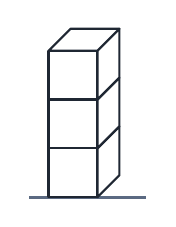
\begin{tikzpicture}[scale=0.62,line join=round]
  \draw[Slate,line width=1pt] (-0.4,0)--(2.0,0);
  \foreach \k/\f/\r in {0/4/1,1/5/3,2/3/1}{
    \begin{scope}[yshift=\k cm]
    \draw[Ink,line width=0.8pt,fill=white] (0,0) rectangle (1,1);
    \draw[Ink,line width=0.8pt,fill=white] (1,0)--(1.45,0.45)--(1.45,1.45)--(1,1)--cycle;
    \begin{scope}[Ink]\lgaPips{\f}\end{scope}
    \begin{scope}[Ink,cm={0.45,0.45,0,1,(1,0)}]\lgaPips{\r}\end{scope}
    \end{scope}}
  \draw[Ink,line width=0.8pt,fill=white] (0,3)--(1,3)--(1.45,3.45)--(0.45,3.45)--cycle;
  \begin{scope}[Ink,cm={1,0,0.45,0.45,(0,3)}]\lgaPips{2}\end{scope}
\end{tikzpicture}
\end{minipage}
\end{probbox}
\probsol{
\textbf{Analysing the problem.} The five hidden horizontal faces are: the bottom face of the top die; the top and bottom faces of the middle
die; the top and bottom faces of the bottom die. We do not need to know each face separately -- we only use ``opposite faces add up to $7$''.
\begin{recallbox}On a standard die the top and bottom faces are opposite, so together they carry $7$ pips.\end{recallbox}
\step{1}{Bottom die and middle die}
For each of them the top and bottom faces are both hidden, and each pair totals $7$. Two dice: $7 + 7 = 14$.
\step{2}{Top die}
The visible top face has $2$ pips, so the (opposite) bottom face has $7 - 2 = 5$ pips, and it is hidden.
\step{3}{Add up}
$14 + 5 = 19$.
\begin{warnbox}(D) $21 = 3\times 7$ forgets that the very top face ($2$ pips) \emph{can be seen}; it is not hidden. (A) $14$ forgets the bottom
face of the top die (also hidden, with $5$ pips).\end{warnbox}
\verify{The six horizontal faces of the three dice total $3\times 7 = 21$; of these only the very top face ($2$ pips) is visible, so the five hidden ones total $21 - 2 = 19$.}
So the answer is \textbf{(C)}.
\ans{(C) $19$}
}

% ---------------------------------------------------------------- Problem 27
\begin{probbox}{27}{\relax}
\begin{minipage}[t]{0.63\linewidth}
The $4\times 4$ grid shown is to be filled so that every row, every column and every thick-bordered $2\times 2$ box contains the digits
$1, 2, 3, 4$. The digit in cell $Q$ is
\choicesL{$1$}{$2$}{$3$}{$4$}{It cannot be determined}
\end{minipage}\hfill
\begin{minipage}[t]{0.33\linewidth}\vspace{4pt}\centering
\lgaFour{2/1/$3$,4/1/$2$,4/2/$1$,1/3/$4$,3/4/$2$,4/4/$Q$}
\end{minipage}
\end{probbox}
\probsol{
\textbf{Analysing the problem.} Cell $Q$ is in row $4$, column $4$ (bottom-right corner), in the bottom-right $2\times 2$ box.
\begin{recallbox}The digit in a cell must differ from every digit already in its row, its column and its $2\times 2$ box.\end{recallbox}
\step{1}{Column $4$}
Column $4$ already has $2$ (row $1$) and $1$ (row $2$). The two remaining cells -- row $3$ column $4$ and cell $Q$ -- must be $3$ and $4$ in
some order.
\step{2}{Row $3$ decides}
Row $3$ already has a $4$ (in column $1$), so row $3$ column $4$ \emph{cannot} be $4$. Hence row $3$ column $4$ is $3$, and $Q = 4$.
\step{3}{Check with the bottom-right box and row $4$}
The bottom-right box contains $3$ (row $3$ column $4$), $2$ (row $4$ column $3$), $Q = 4$, and the remaining cell (row $3$ column $3$) is
$1$ -- all of $1, 2, 3, 4$. Row $4$ has $2$ and $4$, no repeat.
\step{4}{Complete the grid (to be sure there is no contradiction)}
\begin{figC}
  \node at (0,0){\lgaFour{1/1/$1$,2/1/$3$,3/1/$4$,4/1/$2$,1/2/$2$,2/2/$4$,3/2/$3$,4/2/$1$,1/3/$4$,2/3/$2$,3/3/$1$,4/3/$3$,1/4/$3$,2/4/$1$,3/4/$2$,4/4/\textcolor{AnsRed}{$\mathbf{4}$}}};
  \node[font=\small,anchor=west,align=left] at (1.8,0){Row $1$: $1\,3\,4\,2$\\ Row $2$: $2\,4\,3\,1$\\ Row $3$: $4\,2\,1\,3$\\ Row $4$: $3\,1\,2\,4$};
\end{figC}
\verify{Every row, column and $2\times 2$ box contains all of $1, 2, 3, 4$; a computer check confirms this is the only way to fill the grid.}
\begin{warnbox}Looking only at column $4$, $Q$ could be $3$ or $4$, and it is tempting to choose (E). Also look at row $3$ -- a different
region containing a ``neighbour'' of $Q$.\end{warnbox}
So the answer is \textbf{(D)}.
\ans{(D) $4$}
}

% ---------------------------------------------------------------- Problem 28
\begin{probbox}{28}{\relax}
In class 7A, \emph{all} members of the chess club can swim. Lâm cannot swim. Na can swim. Which of the following statements \textbf{must} be true?
\choicesL{Lâm is in the chess club.}{Lâm is not in the chess club.}{Na is in the chess club.}{Na is not in the chess club.}{Everyone in the class who can swim is in the chess club.}
\end{probbox}
\probsol{
\textbf{Analysing the problem.} ``All members of the chess club can swim'' has the form ``every A is a B'' (A: in the chess club, B: can swim).
\begin{recallbox}From ``every A is a B'' we may conclude ``not a B means not an A''; but we may \emph{not} conclude ``a B means an A''.\end{recallbox}
\step{1}{Draw a diagram}
\begin{figC}
  \draw[tmBlue,line width=1pt,fill=tmBlue!8] (0.9,1.1) ellipse (1.9 and 1.2);
  \draw[tmOrange,line width=1pt,fill=tmOrange!15] (0.45,1.0) ellipse (0.85 and 0.62);
  \node[font=\scriptsize,text=tmOrange!70!black] at (0.45,1.05){chess club};
  \node[font=\scriptsize,text=tmBlue!80!black] at (2.0,1.95){can swim};
  \fill[tmGreen!60!black] (2.0,0.75) circle (2.2pt) node[below,font=\scriptsize]{Na?};
  \fill[tmGreen!60!black] (0.5,0.7) circle (2.2pt) node[below,font=\scriptsize]{Na?};
  \fill[AnsRed] (3.6,1.1) circle (2.2pt) node[right,font=\scriptsize]{Lâm};
\end{figC}
The ``chess club'' oval lies entirely inside the ``can swim'' oval.
\step{2}{Lâm}
Lâm cannot swim, so Lâm is \emph{outside} the big oval, and therefore certainly outside the small one: \textbf{Lâm is not in the chess club}.
If Lâm were in the club, Lâm would have to be able to swim -- contradicting the problem (proof by contradiction).
\step{3}{Na}
Na can swim: Na is inside the big oval, but may be inside or outside the small one. So (C) and (D) are each only \emph{possibly} true, not certain.
\step{4}{Statement (E)}
(E) reverses the given statement. The problem says nothing about pupils who can swim but do not play chess, so (E) is not certainly true.
\begin{warnbox}A very common mistake: from ``chess players can all swim'' concluding ``swimmers all play chess''. Think of an example: ``every cat
has four legs'' does not mean ``every four-legged animal is a cat''!\end{warnbox}
So the answer is \textbf{(B)}.
\ans{(B) Lâm is not in the chess club}
}

% ---------------------------------------------------------------- Problem 29
\begin{probbox}{29}{\relax}
Mr Fox lies on Mondays, Tuesdays and Wednesdays and tells the truth on the other days of the week. One day, Fox says: ``Yesterday I lied.''
Which day could it be?
\choicesL{Only Monday.}{Only Thursday.}{Monday or Thursday.}{Wednesday or Thursday.}{Sunday or Monday.}
\end{probbox}
\probsol{
\textbf{Analysing the problem.} Fox can say ``Yesterday I lied'' when:
\begin{itemize}[leftmargin=1.4em,itemsep=0pt,topsep=1pt]
\item he tells the truth today and the statement is true: truthful today, lied yesterday; or
\item he lies today and the statement is false: lying today, truthful yesterday.
\end{itemize}
That is: \textbf{yesterday and today are of different types}.
\begin{recallbox}The day before Monday is Sunday (the week goes round).\end{recallbox}
\step{1}{Make a table}
\begin{center}
\setlength{\tabcolsep}{4pt}
\begin{tabular}{|l|c|c|c|c|c|c|c|}
\hline
\rowcolor{tmBlue!10} Today & Mon & Tue & Wed & Thu & Fri & Sat & Sun \\ \hline
Fox today & L & L & L & T & T & T & T \\ \hline
Fox yesterday & T (Sun) & L & L & L & T & T & T \\ \hline
Different? & \textbf{yes} & -- & -- & \textbf{yes} & -- & -- & -- \\ \hline
\end{tabular}
\end{center}
\step{2}{Check the two days found}
\emph{Monday:} Fox lies; yesterday (Sunday) he told the truth, so ``yesterday I lied'' is false -- indeed a lie. \checkmark\\
\emph{Thursday:} Fox tells the truth; yesterday (Wednesday) he lied, so the statement is true -- indeed the truth. \checkmark
\begin{warnbox}Wednesday: Fox lies, and yesterday (Tuesday) he lied too, so ``yesterday I lied'' is a \emph{true} statement. Someone who is lying
does not say true things, so Wednesday is ruled out -- this is the trap in option (D).\end{warnbox}
So the answer is \textbf{(C)}.
\ans{(C) Monday or Thursday}
}

% ---------------------------------------------------------------- Problem 30
\begin{probbox}{30}{\relax}
Four friends, An, Bách, Cúc and Dung, run a race; no two finish at the same time. Three spectators make predictions:
\begin{itemize}[leftmargin=1.6em,itemsep=0pt,topsep=2pt]
\item Hiếu: ``An comes first, Bách comes second.''
\item Khoa: ``Cúc comes first, Dung comes fourth.''
\item Lan: ``Bách comes third, Dung comes second.''
\end{itemize}
In the end, each spectator got \emph{exactly one} part right. Find the finishing order of the four friends.
\end{probbox}
\probsol{
\textbf{Analysing the problem.} Each prediction has two parts, exactly one of them right. We split into cases using Hiếu's prediction.
\begin{recallbox}``Half-true'' statement: if one part is true the other is false, and if one part is false the other is true.\end{recallbox}
\step{1}{Case 1: ``Bách second'' is true (and ``An first'' is false)}
Look at Lan's prediction. Bách is second, so ``Bách third'' is false; hence the other part ``Dung second'' must be true. But Bách is already
second, so Dung cannot be second too. \textbf{Contradiction} -- this case is ruled out.
\step{2}{Case 2: ``An first'' is true (and ``Bách second'' is false)}
\begin{itemize}[leftmargin=1.4em,itemsep=1pt,topsep=1pt]
\item Khoa: An is first, so ``Cúc first'' is false $\Rightarrow$ ``Dung fourth'' is true.
\item Lan: Dung is fourth, so ``Dung second'' is false $\Rightarrow$ ``Bách third'' is true.
\item Second place is left for Cúc.
\end{itemize}
Order: An (1st), Cúc (2nd), Bách (3rd), Dung (4th).
\step{3}{Check}
\begin{center}
\begin{tabular}{|l|c|c|}
\hline
\rowcolor{tmBlue!10} Spectator & First part & Second part \\ \hline
Hiếu & An first: \textcolor{tmGreen!70!black}{true} & Bách second: \textcolor{AnsRed}{false} \\ \hline
Khoa & Cúc first: \textcolor{AnsRed}{false} & Dung fourth: \textcolor{tmGreen!70!black}{true} \\ \hline
Lan & Bách third: \textcolor{tmGreen!70!black}{true} & Dung second: \textcolor{AnsRed}{false} \\ \hline
\end{tabular}
\end{center}
\begin{tipbox}Choose the prediction to split on so that each case ``triggers'' as many other parts as possible. Here ``Bách second'' clashes
immediately with Lan's ``Dung second'', so case 1 is ruled out very quickly.\end{tipbox}
\begin{parentbox}You can use four slips of paper with the names, line them up as ``1st -- 2nd -- 3rd -- 4th'' and swap them around to test.
Then ask your child: ``Have we tried every case? How can we be sure there is no other answer?'' -- the answer is Step 1.\end{parentbox}
\ans{An 1st, Cúc 2nd, Bách 3rd, Dung 4th.}
}

% ---------------- part c ----------------
% =====================================================================
% Topic 5 — Logic and Puzzles — part c: problems 31–40 (extension)
% =====================================================================
% ---- helper macros for parts c/d of topic 5 (prefix \lgxcd, guarded) ----
% shape codes: 1 = circle, 2 = square, 3 = triangle, 4 = star
\providecommand{\lgxcdShape}[3]{\ifcase#1\or
  \draw[Ink,fill=Slate!35,line width=0.6pt] (#2,#3) circle (0.19);\or
  \draw[Ink,fill=tmBlue!35,line width=0.6pt] ($(#2,#3)+(-0.18,-0.18)$) rectangle ($(#2,#3)+(0.18,0.18)$);\or
  \draw[Ink,fill=tmOrange!45,line width=0.6pt] ($(#2,#3)+(-0.2,0.17)$)--($(#2,#3)+(0.2,0.17)$)--($(#2,#3)+(0,-0.19)$)--cycle;\or
  \draw[Ink,fill=tmGreen!45,line width=0.6pt,shift={(#2,#3)}] (90:0.24) \foreach \lgxcdk in {1,...,9}{ -- ({90+36*\lgxcdk}:{ifthenelse(mod(\lgxcdk,2)==1,0.1,0.24)})} -- cycle;\fi}
% inline shape in text
\providecommand{\lgxcdI}[1]{\tikz[baseline=-0.7ex]{\lgxcdShape{#1}{0}{0}}}
% a row of n shapes centred at the origin: \lgxcdRow{n}{codes}
\providecommand{\lgxcdRow}[2]{\foreach \lgxcdt [count=\lgxcdi] in {#2}{%
  \pgfmathsetmacro\lgxcdxx{(\lgxcdi-(#1+1)/2)*0.48}\lgxcdShape{\lgxcdt}{\lgxcdxx}{0.21}}}
% equal-arm balance at height #1: \lgxcdBal{y}{n left}{codes left}{n right}{codes right}
\providecommand{\lgxcdBal}[5]{\begin{scope}[yshift=#1cm]
  \draw[Ink,line width=1pt] (-2.7,0)--(-0.3,0) (0.3,0)--(2.7,0);
  \draw[Ink,line width=0.9pt] (-1.5,0)--(-1.5,-0.55)--(1.5,-0.55)--(1.5,0);
  \draw[Ink,line width=0.9pt] (-0.18,-0.85)--(0,-0.58)--(0.18,-0.85);
  \begin{scope}[xshift=-1.5cm]\lgxcdRow{#2}{#3}\end{scope}
  \begin{scope}[xshift=1.5cm]\lgxcdRow{#4}{#5}\end{scope}\end{scope}}
% square grid n x n with box lines every #2 rows / #3 columns; #4 = given r/c/v, #5 = filled r/c/v (rows from top)
\providecommand{\lgxcdSud}[5]{\begin{scope}[x=0.62cm,y=0.62cm]
  \foreach \lgxcdi in {0,...,#1}{\draw[Slate!60,line width=0.5pt] (0,\lgxcdi)--(#1,\lgxcdi) (\lgxcdi,0)--(\lgxcdi,#1);}
  \foreach \lgxcdi in {0,#2,...,#1}{\draw[Ink,line width=1.4pt] (0,\lgxcdi)--(#1,\lgxcdi);}
  \foreach \lgxcdi in {0,#3,...,#1}{\draw[Ink,line width=1.4pt] (\lgxcdi,0)--(\lgxcdi,#1);}
  \foreach \lgxcdr/\lgxcdc/\lgxcdv in {#4}{\node[font=\sffamily\bfseries,text=Ink] at (\lgxcdc+0.5,#1-\lgxcdr-0.5){\lgxcdv};}
  \foreach \lgxcdr/\lgxcdc/\lgxcdv in {#5}{\node[font=\sffamily,text=tmBlue] at (\lgxcdc+0.5,#1-\lgxcdr-0.5){\lgxcdv};}
  \end{scope}}

\clearpage
\dividerbar{Extension and challenge}

% ---------------------------------------------------------------- Problem 31
\begin{probbox}{31}{\relax}
On an island, every inhabitant is either a \emph{truth-teller} (always tells the truth) or a \emph{liar} (always lies).
\begin{enumerate}[label=\alph*),leftmargin=1.6em,itemsep=1pt,topsep=2pt]
  \item You meet two inhabitants, Khánh and Lâm. Khánh says: ``Both of us are liars.'' What type is each of them?
  \item You meet three inhabitants, An, Bình and Chi.\\
  An says: ``Bình is a liar.''\\
  Bình says: ``Chi is a liar.''\\
  Chi says: ``An and Bình are both liars.''\\
  What type is each of them?
\end{enumerate}
\end{probbox}
\probsol{
\textbf{Understanding the problem.} Each person has only two possibilities. The safest method is to \emph{assume} one possibility and
check whether the statements fit that assumption. If we reach a contradiction, we rule that possibility out.
\begin{recallbox}Whatever a truth-teller says is \textbf{true}. Whatever a liar says is \textbf{false}. So each statement gives us an
``equation'': \emph{the statement is true} $\Longleftrightarrow$ \emph{the speaker is a truth-teller}.\end{recallbox}
\par\smallskip\textbf{Part a).}
\step{1}{Suppose Khánh is a truth-teller}
Then his statement is true, so Khánh is a liar -- contradicting the assumption. So Khánh \textbf{cannot} be a truth-teller.
\step{2}{Khánh is a liar}
The statement ``Both of us are liars'' is false. It is false when \emph{at least one} of them is not a liar. Khánh is a liar, so the
other one -- Lâm -- must be a truth-teller.
\begin{warnbox}The opposite of ``both are liars'' is \textbf{not} ``both tell the truth'', but ``at least one of them tells the
truth''.\end{warnbox}
\par\smallskip\textbf{Part b).}
\step{3}{Suppose An is a truth-teller}
An's statement is true $\Rightarrow$ Bình is a liar $\Rightarrow$ Bình's statement is false $\Rightarrow$ Chi is a truth-teller
$\Rightarrow$ Chi's statement is true $\Rightarrow$ An is a liar. This contradicts the assumption! Ruled out.
\step{4}{So An is a liar}
An's statement is false $\Rightarrow$ Bình is \emph{not} a liar, i.e.\ Bình is a truth-teller $\Rightarrow$ Bình's statement is true
$\Rightarrow$ Chi is a liar.
\step{5}{Check Chi's statement}
Chi is a liar, so the statement ``An and Bình are both liars'' must be false. Indeed it is false, because Bình is a truth-teller.
There is no contradiction.
\begin{center}
\begin{tabular}{|c|c|l|c|}
\hline
\rowcolor{tmBlue!10} Person & Type & Statement & True/false\\ \hline
An & liar & Bình is a liar & false \\ \hline
Bình & truth-teller & Chi is a liar & true\\ \hline
Chi & liar & An and Bình are both liars & false\\ \hline
\end{tabular}
\end{center}
\verify{In the table, every truth-teller makes a true statement and every liar a false one. We have also seen that ``An is a
truth-teller'' is impossible, so this is the only solution.}
\ans{a) Khánh is a liar, Lâm a truth-teller;\quad b) An and Chi are liars, Bình is a truth-teller}
}

% ---------------------------------------------------------------- Problem 32
\begin{probbox}{32}{\relax}
Mai lies on Mondays, Tuesdays and Wednesdays and tells the truth on the other days of the week. Hùng lies on Thursdays, Fridays and
Saturdays and tells the truth on the other days. One day, both of them say: ``Yesterday was a day on which I lie.'' Which day of the
week is it?
\end{probbox}
\probsol{
\textbf{Understanding the problem.} The statement ``Yesterday was a day on which I lie'' may be true or false depending on the day.
For each person we find the days on which they \emph{could} say it, then take the day common to both.
\begin{recallbox}On a truth day the statement must be true; on a lying day the statement must be false.\end{recallbox}
\step{1}{Table for Mai (lies Mon, Tue, Wed)}
\begin{center}\small
\begin{tabular}{|l|c|c|c|c|c|c|c|}
\hline
\rowcolor{tmBlue!10} Today & Mon & Tue & Wed & Thu & Fri & Sat & Sun\\ \hline
Mai today & lies & lies & lies & truth & truth & truth & truth\\ \hline
Mai yesterday & truth (Sun) & lies & lies & lies & truth & truth & truth\\ \hline
Statement true? & no & yes & yes & yes & no & no & no\\ \hline
Can Mai say it? & \textbf{yes} & no & no & \textbf{yes} & no & no & no\\ \hline
\end{tabular}
\end{center}
Mai can say it when she lies today and the statement is false (Monday), or when she tells the truth today and the statement is true
(Thursday).
\step{2}{Table for Hùng (lies Thu, Fri, Sat)}
\begin{center}\small
\begin{tabular}{|l|c|c|c|c|c|c|c|}
\hline
\rowcolor{tmBlue!10} Today & Mon & Tue & Wed & Thu & Fri & Sat & Sun\\ \hline
Hùng today & truth & truth & truth & lies & lies & lies & truth\\ \hline
Hùng yesterday & truth & truth & truth & truth & lies & lies & lies\\ \hline
Statement true? & no & no & no & no & yes & yes & yes\\ \hline
Can Hùng say it? & no & no & no & \textbf{yes} & no & no & \textbf{yes}\\ \hline
\end{tabular}
\end{center}
Hùng can say it on Thursday or Sunday.
\step{3}{The common day}
Mai: $\{$Monday, Thursday$\}$; Hùng: $\{$Thursday, Sunday$\}$. The only common day is \textbf{Thursday}.
\begin{tipbox}Quick rule: a person can say ``Yesterday I lied'' only on a \emph{switch day} (yesterday and today are of different
types): the first lying day, or the first day back to telling the truth.\end{tipbox}
\verify{Thursday: Mai tells the truth, and yesterday (Wednesday) she lied -- the statement is true, consistent. Hùng lies, and
yesterday (Wednesday) he told the truth -- the statement is false, consistent with Hùng lying today.}
\ans{Thursday}
}

% ---------------------------------------------------------------- Problem 33
\begin{probbox}{33}{\relax}
Six friends Lan, Minh, Nam, Oanh, Phúc and Quân run a race. No two of them finish at the same time. We know that:
\begin{itemize}[leftmargin=1.4em,itemsep=0pt,topsep=2pt]
  \item Minh finishes after Lan but before Nam;
  \item Oanh finishes after Nam;
  \item Phúc finishes \emph{immediately after} Lan;
  \item Quân is neither first nor last, and Quân finishes before Minh.
\end{itemize}
Find the finishing order of the six friends. Who finishes third?
\end{probbox}
\probsol{
\textbf{Understanding the problem.} We have ``before -- after'' conditions. A good method is to join them into a \emph{chain} and then
insert the remaining friends one by one. Write $X \to Y$ for ``$X$ finishes before $Y$''.
\step{1}{Join conditions 1 and 2}
Lan $\to$ Minh $\to$ Nam and Nam $\to$ Oanh, so: \ Lan $\to$ Minh $\to$ Nam $\to$ Oanh.
\step{2}{Insert Phúc}
Phúc finishes \emph{immediately after} Lan, i.e.\ nobody comes between Lan and Phúc: \ Lan, Phúc $\to$ Minh $\to$ Nam $\to$ Oanh.
\step{3}{Insert Quân}
Quân finishes before Minh, so Quân is in one of these places: before Lan, or between Phúc and Minh (he may not come between Lan and
Phúc). But Quân is not first, so he is not before Lan. Hence:
\[ \text{Lan} \to \text{Phúc} \to \text{Quân} \to \text{Minh} \to \text{Nam} \to \text{Oanh}. \]
\begin{figC}
\foreach \n/\x in {Lan/0,Phúc/1,Quân/2,Minh/3,Nam/4,Oanh/5}{
  \node[draw=tmBlue,fill=tmBlue!8,rounded corners=3pt,minimum width=1.5cm,minimum height=0.7cm] at (\x*1.9,0){\n};}
\foreach \x [count=\k] in {0,...,5}{\node[font=\scriptsize,text=Slate] at (\x*1.9,-0.6){place \k};}
\foreach \x in {0,...,4}{\draw[->,tmBlue,thick] (\x*1.9+0.78,0)--(\x*1.9+1.12,0);}
\end{figC}
\step{4}{Check every condition again}
Minh (4th) is after Lan (1st) and before Nam (5th): true. Oanh (6th) is after Nam: true. Phúc (2nd) is immediately after Lan: true.
Quân is 3rd -- not first, not last, before Minh: true.
\begin{warnbox}If you forget the word ``immediately'', Quân could come between Lan and Phúc and the problem would have two answers. Read
every word of each condition carefully!\end{warnbox}
\verify{We tried every possible position for Quân; only one order satisfies all four conditions.}
\ans{Lan, Phúc, Quân, Minh, Nam, Oanh; Quân finishes third}
}

% ---------------------------------------------------------------- Problem 34
\begin{probbox}{34}{\relax}
Five friends Hà, Khoa, Linh, My and Tùng sit in a row of $5$ chairs numbered $1, 2, 3, 4, 5$ from left to right. We know that:
Hà and Khoa sit next to each other; Linh and My do \emph{not} sit next to each other; Tùng sits at one end of the row (chair $1$ or
chair $5$).
\begin{enumerate}[label=\alph*),leftmargin=1.6em,itemsep=1pt,topsep=2pt]
  \item How many seating arrangements satisfy these conditions?
  \item Which of the following statements is \emph{certainly true}?\\
  (1) Linh sits at one end of the row. \quad (2) Hà does not sit at an end of the row. \quad (3) Khoa sits in chair $3$.
  \item If we also know that Linh sits in chair $1$ and Hà sits to the left of Khoa, find each friend's seat.
\end{enumerate}
\end{probbox}
\probsol{
\textbf{Understanding the problem.} Start with the ``tightest'' condition (Tùng has only $2$ places), then look at the $4$ remaining
chairs.
\step{1}{Case: Tùng sits in chair 5}
The other four sit in chairs $1, 2, 3, 4$. The pair Hà -- Khoa takes two adjacent chairs: $(1,2)$, $(2,3)$ or $(3,4)$.
\begin{itemize}[leftmargin=1.4em,itemsep=0pt,topsep=1pt]
  \item Hà -- Khoa in chairs $(1,2)$: Linh and My must sit in chairs $3, 4$ -- next to each other, \textbf{impossible}.
  \item Hà -- Khoa in chairs $(3,4)$: Linh and My sit in chairs $1, 2$ -- next to each other, \textbf{impossible}.
  \item Hà -- Khoa in chairs $(2,3)$: Linh and My sit in chairs $1$ and $4$ -- not next to each other, \textbf{possible}.
\end{itemize}
In the possible case, Hà and Khoa can swap ($2$ ways) and Linh and My can swap ($2$ ways): $2\times 2 = 4$ ways.
\step{2}{Case: Tùng sits in chair 1}
Exactly the same (turn the row around): Hà -- Khoa in chairs $(3,4)$, Linh and My in chairs $2$ and $5$: also $4$ ways.
\step{3}{Total number of ways}
$4 + 4 = 8$ ways.
\begin{recallbox}\textbf{Multiplication rule:} if a task consists of consecutive steps, step 1 in $m$ ways and step 2 in $n$ ways, then
the task can be done in $m\times n$ ways. \textbf{Addition rule:} separate cases are added.\end{recallbox}
\step{4}{Part b): check each statement}
\begin{center}\small
\begin{tabular}{|c|c|c|c|c|}
\hline
\rowcolor{tmBlue!10} Chair 1 & Chair 2 & Chair 3 & Chair 4 & Chair 5\\ \hline
Linh/My & Hà/Khoa & Hà/Khoa & My/Linh & Tùng\\ \hline
Tùng & Linh/My & Hà/Khoa & Hà/Khoa & My/Linh\\ \hline
\end{tabular}
\end{center}
(1) False: when Tùng is in chair 1, Linh may sit in chair 2. \ (2) \textbf{True}: in both rows, Hà and Khoa are always in middle chairs
($2, 3$ or $3, 4$). \ (3) False: Khoa may sit in chair $2$ or chair $4$.
\step{5}{Part c)}
Linh is in chair $1$, so Tùng is not in chair $1$; Tùng is in chair $5$ (first row of the table). Then My is in chair $4$ and Hà --
Khoa in chairs $2, 3$; Hà is to the left of Khoa, so Hà is in chair $2$ and Khoa in chair $3$.
\verify{Linh(1), Hà(2), Khoa(3), My(4), Tùng(5): Hà and Khoa are adjacent; Linh in chair 1 and My in chair 4 are not adjacent; Tùng
is at an end. Correct.}
\ans{a) $8$ ways;\quad b) statement (2);\quad c) Linh -- Hà -- Khoa -- My -- Tùng (chairs 1 to 5)}
}

% ---------------------------------------------------------------- Problem 35
\begin{probbox}{35}{\relax}
Number the letters $A, B, C, \dots, Z$ (the $26$-letter English alphabet) as $0, 1, 2, \dots, 25$. The \emph{Caesar cipher with key
$k$} replaces each letter with number $x$ by the letter whose number is the \emph{remainder} of $x + k$ when divided by $26$
(spaces are kept).
\begin{figC}
\foreach \L [count=\i from 0] in {A,B,C,D,E,F,G,H,I,J,K,L,M,N,O,P,Q,R,S,T,U,V,W,X,Y,Z}{
  \node[font=\sffamily\small\bfseries,text=Ink] at ({90-\i*360/26}:2.15){\L};
  \node[font=\sffamily\tiny,text=tmBlue] at ({90-\i*360/26}:1.65){\i};}
\draw[Line,line width=0.8pt] (0,0) circle (1.9);
\draw[->,tmOrange,line width=1pt] (110:1.2) arc (110:30:1.2);
\node[font=\scriptsize,text=tmOrange!80!black,align=center] at (0,0){move\\clockwise};
\end{figC}
\begin{enumerate}[label=\alph*),leftmargin=1.6em,itemsep=1pt,topsep=2pt]
  \item Encrypt the text \textsf{TOAN HOC} with key $k = 5$.
  \item Decrypt the text \textsf{OVJ CBP}, knowing that the key is $k = 7$.
  \item In a message, the word \textsf{BAN} was encrypted as \textsf{QPC}. Find the key $k$ (with $0 \le k \le 25$), then decrypt the
  word \textsf{HPJ} from the same message.
  \item A message is encrypted with key $10$, and the result is encrypted once more with key $20$. These two encryptions together
  are the same as \emph{one} encryption with which key?
  \item Tú encrypts a word with key $4$, then encrypts the result with key $4$ again, and so on. After how many encryptions, at least,
  does Tú get back exactly the original word?
\end{enumerate}
\end{probbox}
\probsol{
\textbf{Understanding the problem.} When adding the key takes us past $25$, we ``wrap around'' to the start of the alphabet -- that is
exactly taking the \emph{remainder on division by $26$}. Decrypting is the reverse: \emph{subtract} the key (if the result is
negative, add $26$).
\begin{recallbox}The remainder of $a$ on division by $26$ is the number $r$ with $0 \le r \le 25$ such that $a - r$ is divisible by
$26$. Examples: $30$ leaves remainder $4$; \ $-6$ ``leaves remainder'' $20$, because $-6 + 26 = 20$.\end{recallbox}
\step{1}{Part a): encrypt \textsf{TOAN HOC} with $k = 5$}
\begin{center}\small
\begin{tabular}{|c|c|c|c|c|c|c|c|}
\hline
\rowcolor{tmBlue!10} Plain letter & T & O & A & N & H & O & C\\ \hline
Number $x$ & $19$ & $14$ & $0$ & $13$ & $7$ & $14$ & $2$\\ \hline
$x + 5$ & $24$ & $19$ & $5$ & $18$ & $12$ & $19$ & $7$\\ \hline
Cipher letter & Y & T & F & S & M & T & H\\ \hline
\end{tabular}
\end{center}
Result: \textsf{YTFS MTH}. (No number exceeds $25$ here, so no wrapping is needed yet.)
\step{2}{Part b): decrypt \textsf{OVJ CBP} with $k = 7$ (subtract $7$)}
\begin{center}\small
\begin{tabular}{|c|c|c|c|c|c|c|}
\hline
\rowcolor{tmBlue!10} Cipher letter & O & V & J & C & B & P\\ \hline
Number & $14$ & $21$ & $9$ & $2$ & $1$ & $15$\\ \hline
Number $- 7$ & $7$ & $14$ & $2$ & $-5 \to 21$ & $-6 \to 20$ & $8$\\ \hline
Plain letter & H & O & C & V & U & I\\ \hline
\end{tabular}
\end{center}
Original text: \textsf{HOC VUI} (Vietnamese for ``fun learning''). Note: $2 - 7 = -5$, adding $26$ gives $21$ (the letter V).
\step{3}{Part c): find the key from the pair \textsf{BAN} $\to$ \textsf{QPC}}
B ($1$) becomes Q ($16$), so $k = 16 - 1 = 15$. Check: A ($0$) $\to 0 + 15 = 15$ (P), correct; N ($13$) $\to 13 + 15 = 28$, remainder
$2$ on division by $26$ (C), correct. So $k = 15$.\\
Decrypt \textsf{HPJ} (subtract $15$): H $= 7$, $7 - 15 = -8 \to 18$ (S); \ P $= 15 \to 0$ (A); \ J $= 9$, $9 - 15 = -6 \to 20$ (U).
The original word is \textsf{SAU}.
\step{4}{Part d): two encryptions in a row}
Each letter gets $10$ added and then $20$ added, i.e.\ $30$ added. Since $30$ leaves remainder $4$ on division by $26$, ``add $30$ and
take the remainder'' is exactly the same as ``add $4$ and take the remainder''. The two encryptions equal \textbf{one encryption with
key $4$}.
\step{5}{Part e): repeated encryption with key $4$}
After $n$ encryptions, every letter has moved $4n$ places. To get back to the original letter we must go round a whole number of
times, i.e.\ $4n$ must be divisible by $26$. Try $n = 1, 2, 3, \dots$: \ $4n = 4, 8, 12, \dots$ The smallest (non-zero) $4n$
divisible by $26$ is $\text{LCM}(4, 26) = 52$, which gives $n = 52 \div 4 = 13$.
\begin{recallbox}$4n$ is divisible by $26 = 2\times 13$ $\Leftrightarrow$ $2n$ is divisible by $13$ $\Leftrightarrow$ $n$ is divisible
by $13$ (because $13$ is a prime that does not divide $2$).\end{recallbox}
\begin{tipbox}With key $13$ you only need $2$ encryptions to get back ($2\times 13 = 26$). Encrypting twice with key $13$ is the same as
decrypting!\end{tipbox}
\verify{Part a): decrypting \textsf{YTFS MTH} by subtracting $5$ gives back \textsf{TOAN HOC}. Part c): \textsf{SAU} encrypted with key
$15$: S $18 + 15 = 33 \to 7$ (H), A $\to 15$ (P), U $20 + 15 = 35 \to 9$ (J). Indeed \textsf{HPJ}.}
\ans{a) \textsf{YTFS MTH};\ b) \textsf{HOC VUI};\ c) $k = 15$, \textsf{SAU};\ d) key $4$;\ e) $13$ times}
}

% ---------------------------------------------------------------- Problem 36
\begin{probbox}{36}{\stars{1}}
Again number $A = 0, B = 1, \dots, Z = 25$. A \emph{multiplicative cipher} replaces the letter with number $x$ by the letter whose number
is the remainder of $3x + 2$ on division by $26$.
\begin{enumerate}[label=\alph*),leftmargin=1.6em,itemsep=1pt,topsep=2pt]
  \item Encrypt the word \textsf{MEO}.
  \item Decrypt the word \textsf{ECS}.
  \item Nhật suggests using $2x + 2$ instead of $3x + 2$. Find two different letters with the same cipher letter. Why does that make
  decryption impossible?
  \item Explain why, with $3x + 2$, two different letters always get two different cipher letters.
\end{enumerate}
\end{probbox}
\probsol{
\textbf{Understanding the problem.} This cipher does not just ``shift'': it also multiplies and then takes the remainder. Encrypting is
easy (compute directly); to decrypt we need $x$ when we know the remainder of $3x + 2$ -- we use the trick ``add $26$ until the number
is divisible by $3$''.
\step{1}{Part a): encrypt \textsf{MEO}}
M $= 12$: $3\cdot 12 + 2 = 38$, remainder $12$ on division by $26$ $\to$ M.\\
E $= 4$: $3\cdot 4 + 2 = 14$ $\to$ O.\\
O $= 14$: $3\cdot 14 + 2 = 44$, remainder $18$ $\to$ S.\\
Result: \textsf{MOS}. (Fun fact: M is encrypted as itself.)
\step{2}{Part b): decrypt \textsf{ECS}}
For a cipher letter with number $y$ we need $x$ ($0 \le x \le 25$) such that $3x + 2$ leaves remainder $y$, i.e.\ $3x = y - 2$, or
$y - 2 + 26$, or $y - 2 + 52$ (try them in turn and take the one divisible by $3$).
\begin{center}\small
\begin{tabular}{|c|c|c|c|c|}
\hline
\rowcolor{tmBlue!10} Cipher letter & $y$ & Try $y - 2,\ y + 24,\ y + 50$ & $3x$ & Plain letter\\ \hline
E & $4$ & $2$ (no), $28$ (no), $54$ (divisible) & $54 \Rightarrow x = 18$ & S\\ \hline
C & $2$ & $0$ (divisible) & $0 \Rightarrow x = 0$ & A\\ \hline
S & $18$ & $16$ (no), $42$ (divisible) & $42 \Rightarrow x = 14$ & O\\ \hline
\end{tabular}
\end{center}
The original word is \textsf{SAO}.
\step{3}{Part c): why $2x + 2$ does not work}
A $= 0$: $2\cdot 0 + 2 = 2$ $\to$ C. \quad N $= 13$: $2\cdot 13 + 2 = 28$, remainder $2$ $\to$ C.\\
Both A and N become C. When the receiver sees a C, they cannot tell whether the original letter was A or N, so decryption is not
certain. (In fact every number $2x + 2$ is even, so there are only $13$ cipher letters for $26$ plain letters -- some pairs must
coincide.)
\step{4}{Part d): why $3x + 2$ never collides}
\begin{proofbox}Suppose two letters $x$ and $z$ (with $0 \le z < x \le 25$) have the same cipher letter. Then $3x + 2$ and $3z + 2$ leave
the same remainder on division by $26$, so their difference $3(x - z)$ is divisible by $26$. But $3$ and $26$ have no common divisor
greater than $1$, so $x - z$ must be divisible by $26$. However $0 < x - z \le 25$ -- not divisible by $26$. Contradiction. So
different letters always get different cipher letters.\end{proofbox}
\begin{warnbox}With $2x + 2$, the argument breaks down here: $2(x - z)$ is divisible by $26$ as soon as $x - z$ is divisible by $13$,
for example $x - z = 13$ (A and N).\end{warnbox}
\verify{Encrypt \textsf{SAO} again: S $3\cdot 18 + 2 = 56 \to 56 - 52 = 4$ (E); A $\to 2$ (C); O $\to 44 - 26 = 18$ (S). We get
\textsf{ECS}, correct.}
\ans{a) \textsf{MOS};\ b) \textsf{SAO};\ c) A and N both become C;\ d) see the proof}
}

% ---------------------------------------------------------------- Problem 37
\begin{probbox}{37}{\relax}
In a $3\times 3$ \emph{magic square}, the numbers in every row, every column and both diagonals have the same sum (called the
\emph{magic sum} $M$).
\begin{enumerate}[label=\alph*),leftmargin=1.6em,itemsep=1pt,topsep=2pt]
  \item Let $c$ be the number in the centre cell. Prove that $M = 3c$.
  \item Fill in the empty cells of the magic square below.
\end{enumerate}
\begin{figC}
\lgxcdSud{3}{3}{3}{0/0/9,0/1/19,2/2/13}{}
\end{figC}
\end{probbox}
\probsol{
\textbf{Understanding the problem.} In part b) only three numbers are known; we know neither the centre nor $M$. Part a) is the ``key'':
it links the centre number to $M$.
\step{1}{Part a): add the four lines through the centre}
Name the cells:
\begin{figC}
\lgxcdSud{3}{3}{3}{0/0/$a$,0/1/$b$,0/2/$d$,1/0/$e$,1/1/$c$,1/2/$f$,2/0/$g$,2/1/$h$,2/2/$i$}{}
\end{figC}
Four lines pass through the centre: the middle row $e + c + f$, the middle column $b + c + h$, and the two diagonals $a + c + i$ and
$d + c + g$. Adding these four sums:
\[ (e + c + f) + (b + c + h) + (a + c + i) + (d + c + g) = 4M. \]
On the left, each outer cell appears exactly \emph{once}, while the centre $c$ appears \emph{four} times. So the left side equals
(sum of all $9$ cells) $+\, 3c$.
\begin{proofbox}The sum of all $9$ cells is the sum of the three rows, i.e.\ $3M$. Therefore $3M + 3c = 4M$, which gives $3c = M$.\end{proofbox}
\step{2}{Part b): find the centre}
The main diagonal passes through $9$, the centre $c$ and $13$: \ $9 + c + 13 = M = 3c$. So $22 = 2c$, $c = 11$ and $M = 33$.
\step{3}{Fill the cells one by one (each time choose a line with only one cell missing)}
\begin{itemize}[leftmargin=1.4em,itemsep=0pt,topsep=1pt]
  \item Top row: $33 - 9 - 19 = 5$ (top right corner).
  \item Other diagonal: $33 - 5 - 11 = 17$ (bottom left corner).
  \item Left column: $33 - 9 - 17 = 7$; \quad middle row: $33 - 7 - 11 = 15$.
  \item Bottom row: $33 - 17 - 13 = 3$.
\end{itemize}
\begin{figC}
\lgxcdSud{3}{3}{3}{0/0/9,0/1/19,2/2/13}{0/2/5,1/0/7,1/1/11,1/2/15,2/0/17,2/1/3}
\end{figC}
\verify{Middle column $19 + 11 + 3 = 33$; right column $5 + 15 + 13 = 33$; middle row $7 + 11 + 15 = 33$; the diagonals $9 + 11 + 13$ and
$5 + 11 + 17$ both equal $33$.}
\begin{tipbox}The result $M = 3c$ holds for \emph{every} $3\times 3$ magic square, even with negative numbers or fractions.\end{tipbox}
\ans{a) see the proof;\quad b) top row $9, 19, 5$; middle row $7, 11, 15$; bottom row $17, 3, 13$}
}

% ---------------------------------------------------------------- Problem 38
\begin{probbox}{38}{\relax}
The three equal-arm balances below are all balanced. Objects of the same shape have the same mass.
\begin{figC}
\lgxcdBal{0}{2}{2,3}{5}{1,1,1,1,1}
\lgxcdBal{-1.5}{2}{3,3}{4}{1,1,1,1}
\lgxcdBal{-3}{2}{4,1}{2}{2,2}
\node[font=\small\bfseries,text=Slate] at (-3.3,0){(1)};
\node[font=\small\bfseries,text=Slate] at (-3.3,-1.5){(2)};
\node[font=\small\bfseries,text=Slate] at (-3.3,-3){(3)};
\end{figC}
\begin{enumerate}[label=\alph*),leftmargin=1.6em,itemsep=1pt,topsep=2pt]
  \item How many \lgxcdI{1} does each of \lgxcdI{3}, \lgxcdI{2}, \lgxcdI{4} weigh?
  \item How many \lgxcdI{3} are needed to balance \lgxcdI{4}\,\lgxcdI{4}\,\lgxcdI{2}\,\lgxcdI{2}?
  \item Each \lgxcdI{1} weighs $12$ g. How many grams do the three objects \lgxcdI{4}\,\lgxcdI{3}\,\lgxcdI{2} weigh altogether?
\end{enumerate}
\end{probbox}
\probsol{
\textbf{Understanding the problem.} Choose \lgxcdI{1} as the ``unit of measure''. Look for a balance with only \emph{one kind} of unknown
object, solve it first, and substitute into the other balances.
\begin{recallbox}A balanced scale is like an equation. We may remove (or add) identical objects on both pans, or split both pans into
equal parts, and the scale stays balanced.\end{recallbox}
\step{1}{Balance (2): find \lgxcdI{3}}
Two \lgxcdI{3} balance four \lgxcdI{1}. Halve each pan: one \lgxcdI{3} balances two \lgxcdI{1}. \quad \lgxcdI{3} $= 2$ \lgxcdI{1}.
\step{2}{Balance (1): find \lgxcdI{2}}
\lgxcdI{2}\,\lgxcdI{3} balance five \lgxcdI{1}. Replace \lgxcdI{3} by two \lgxcdI{1}: \lgxcdI{2} together with two \lgxcdI{1} balance
five \lgxcdI{1}. Remove two \lgxcdI{1} from each pan: \lgxcdI{2} $= 3$ \lgxcdI{1}.
\step{3}{Balance (3): find \lgxcdI{4}}
\lgxcdI{4}\,\lgxcdI{1} balance two \lgxcdI{2}, i.e.\ $2\times 3 = 6$ \lgxcdI{1}. Remove one \lgxcdI{1} from each pan:
\lgxcdI{4} $= 5$ \lgxcdI{1}.
\step{4}{Part b)}
\lgxcdI{4}\,\lgxcdI{4}\,\lgxcdI{2}\,\lgxcdI{2} weigh as much as $5 + 5 + 3 + 3 = 16$ \lgxcdI{1}. Each \lgxcdI{3} equals $2$
\lgxcdI{1}, so we need $16 \div 2 = 8$ objects \lgxcdI{3}.
\step{5}{Part c)}
\lgxcdI{4}\,\lgxcdI{3}\,\lgxcdI{2} weigh as much as $5 + 2 + 3 = 10$ \lgxcdI{1}, i.e.\ $10\times 12 = 120$ g.
\begin{tipbox}If we call the masses $t$ (triangle), $q$ (square), $s$ (star), $o$ (circle), the three balances are three equations:
$q + t = 5o$; \ $2t = 4o$; \ $s + o = 2q$. Solving in turn gives $t = 2o$, $q = 3o$, $s = 5o$.\end{tipbox}
\verify{Balance (1): $3 + 2 = 5$. Balance (2): $2 + 2 = 4$. Balance (3): $5 + 1 = 6 = 3 + 3$. All three balances are balanced.}
\ans{a) \lgxcdI{3} $= 2$, \lgxcdI{2} $= 3$, \lgxcdI{4} $= 5$ objects \lgxcdI{1};\quad b) $8$ objects \lgxcdI{3};\quad c) $120$ g}
}

% ---------------------------------------------------------------- Problem 39
\begin{probbox}{39}{\relax}
The ``wheel'' below has $7$ circles: one at the hub and $6$ on the rim, forming $3$ straight ``spokes'' of $3$ circles each (two opposite
circles on the rim and the hub). Place the numbers $1, 2, 3, 4, 5, 6, 7$, one in each circle, so that the three numbers on each spoke
have the same sum $S$.
\begin{figC}
\foreach \a in {90,150,210}{\draw[Ink,line width=0.9pt] (\a:1.5)--(\a+180:1.5);}
\draw[Line,line width=0.8pt] (0,0) circle (1.5);
\foreach \a in {30,90,...,330}{\draw[Ink,fill=white,line width=0.9pt] (\a:1.5) circle (0.3);}
\draw[Ink,fill=tmBlue!12,line width=0.9pt] (0,0) circle (0.3);
\end{figC}
\begin{enumerate}[label=\alph*),leftmargin=1.6em,itemsep=1pt,topsep=2pt]
  \item Let $c$ be the number at the hub. Prove that $3S = 28 + 2c$.
  \item Deduce that the hub can only be $1$, $4$ or $7$. In each case find $S$ and give one arrangement.
\end{enumerate}
\end{probbox}
\probsol{
\textbf{Understanding the problem.} This is the ``count twice'' technique: add all the spokes and see how many times each circle is
counted.
\step{1}{Part a): add the three spokes}
The three spokes total $S + S + S = 3S$. In this sum every rim circle is counted \emph{once} (each rim circle lies on only one spoke),
while the hub is counted \emph{three} times. So
\[ 3S = (1 + 2 + \dots + 7) + 2c = 28 + 2c. \]
\begin{recallbox}$1 + 2 + 3 + 4 + 5 + 6 + 7 = 28$. The hub already appears once in the total $28$, so we only add $2c$ (the other two
times).\end{recallbox}
\step{2}{Part b): which values can $c$ take?}
$3S$ is divisible by $3$, so $28 + 2c$ must be divisible by $3$. Try $c = 1, 2, \dots, 7$:
\begin{center}\small
\begin{tabular}{|c|c|c|c|c|c|c|c|}
\hline
\rowcolor{tmBlue!10} $c$ & $1$ & $2$ & $3$ & $4$ & $5$ & $6$ & $7$\\ \hline
$28 + 2c$ & $\mathbf{30}$ & $32$ & $34$ & $\mathbf{36}$ & $38$ & $40$ & $\mathbf{42}$\\ \hline
Divisible by $3$? & yes & no & no & yes & no & no & yes\\ \hline
\end{tabular}
\end{center}
So $c \in \{1; 4; 7\}$, giving $S = 10$; $12$; $14$ respectively.
\step{3}{Concrete arrangements}
On each spoke the two opposite circles must add up to $S - c$, so we split the remaining $6$ numbers into $3$ pairs with equal sums.
\begin{itemize}[leftmargin=1.4em,itemsep=0pt,topsep=1pt]
  \item $c = 1$, $S = 10$: pairs with sum $9$: $(2, 7), (3, 6), (4, 5)$.
  \item $c = 4$, $S = 12$: pairs with sum $8$: $(1, 7), (2, 6), (3, 5)$.
  \item $c = 7$, $S = 14$: pairs with sum $7$: $(1, 6), (2, 5), (3, 4)$.
\end{itemize}
\begin{figC}
\foreach \cx/\cc/\p in {0/1/{2,3,4,7,6,5},4/4/{1,2,3,7,6,5},8/7/{1,2,3,6,5,4}}{
 \begin{scope}[xshift=\cx cm,scale=0.7]
  \foreach \a in {90,150,210}{\draw[Ink,line width=0.8pt] (\a:1.5)--(\a+180:1.5);}
  \foreach \v [count=\k from 0] in \p{\draw[Ink,fill=white,line width=0.8pt] (90+\k*60:1.5) circle (0.33);
     \node[font=\sffamily\small\bfseries,text=tmBlue] at (90+\k*60:1.5){\v};}
  \draw[Ink,fill=tmBlue!12,line width=0.8pt] (0,0) circle (0.33); \node[font=\sffamily\small\bfseries] at (0,0){\cc};
 \end{scope}}
\node[font=\small] at (0,-1.55){$S = 10$}; \node[font=\small] at (4,-1.55){$S = 12$}; \node[font=\small] at (8,-1.55){$S = 14$};
\end{figC}
\begin{warnbox}Do not assume ``the hub must be the middle number of the list ($4$)''. Both $1$ and $7$ can also go at the hub!\end{warnbox}
\verify{$S = 10$: $1 + 2 + 7 = 1 + 3 + 6 = 1 + 4 + 5 = 10$. \ $S = 12$: $4 + 1 + 7 = 4 + 2 + 6 = 4 + 3 + 5 = 12$. \
$S = 14$: $7 + 1 + 6 = 7 + 2 + 5 = 7 + 3 + 4 = 14$.}
\ans{a) see the proof;\quad b) $c = 1, S = 10$;\ \ $c = 4, S = 12$;\ \ $c = 7, S = 14$ (arrangements as in the figure)}
}

% ---------------------------------------------------------------- Problem 40
\begin{probbox}{40}{\stars{1}}
Place the numbers $1, 2, 3, 4, 5, 6$, one in each circle on the sides of the triangle (three circles at the vertices, three at the
midpoints of the sides), so that the three numbers on each side have the same sum $S$.
\begin{figC}
\draw[Ink,line width=0.9pt] (0,2.2)--(-2.2,-1.3)--(2.2,-1.3)--cycle;
\foreach \p in {(0,2.2),(-2.2,-1.3),(2.2,-1.3),(-1.1,0.45),(1.1,0.45),(0,-1.3)}{\draw[Ink,fill=white,line width=0.9pt] \p circle (0.3);}
\end{figC}
\begin{enumerate}[label=\alph*),leftmargin=1.6em,itemsep=1pt,topsep=2pt]
  \item Let $V$ be the sum of the three numbers at the vertices. Prove that $3S = 21 + V$. Hence find all possible values of $S$.
  \item For each value of $S$, give one arrangement.
  \item When $S = 10$, which three numbers are at the vertices? Explain why there is no other possibility.
\end{enumerate}
\end{probbox}
\probsol{
\textbf{Understanding the problem.} As in Problem 39, we ``count twice'': each vertex circle lies on \emph{two} sides, each midpoint
circle on \emph{one} side.
\step{1}{Part a): add the three sides}
The three sides total $3S$. In this sum each midpoint number is counted once and each vertex number twice. So
\[ 3S = (1 + 2 + 3 + 4 + 5 + 6) + V = 21 + V. \]
\step{2}{Bounds on $V$}
$V$ is the sum of three different numbers from $1, \dots, 6$: at least $1 + 2 + 3 = 6$, at most $4 + 5 + 6 = 15$. Also $21 + V$ is
divisible by $3$, and $21$ is divisible by $3$, so $V$ is divisible by $3$:
\[ V \in \{6;\ 9;\ 12;\ 15\} \quad\Rightarrow\quad S = \frac{21 + V}{3} \in \{9;\ 10;\ 11;\ 12\}. \]
\begin{recallbox}If $a$ is divisible by $3$ and $a + b$ is divisible by $3$, then $b$ is also divisible by $3$.\end{recallbox}
\step{3}{Part b): one arrangement for each $S$}
Choose three vertex numbers with sum $V$; then subtract the sum of the two end numbers of each side from $S$ to get the number at the
middle of that side.
\begin{figC}
\foreach \cx/\S/\t/\l/\r/\ml/\mr/\mb in {0/9/1/2/3/6/5/4, 3.6/10/1/3/5/6/4/2, 7.2/11/2/4/6/5/3/1, 10.8/12/4/5/6/3/2/1}{
 \begin{scope}[xshift=\cx cm,scale=0.62]
  \draw[Ink,line width=0.8pt] (0,2.2)--(-2.2,-1.3)--(2.2,-1.3)--cycle;
  \foreach \p/\v/\col in {(0,2.2)/\t/Ink,(-2.2,-1.3)/\l/Ink,(2.2,-1.3)/\r/Ink,(-1.1,0.45)/\ml/tmBlue,(1.1,0.45)/\mr/tmBlue,(0,-1.3)/\mb/tmBlue}{
    \draw[Ink,fill=white,line width=0.8pt] \p circle (0.36); \node[font=\sffamily\small\bfseries,text=\col] at \p {\v};}
  \node[font=\small] at (0,-2.2){$S = \S$};
 \end{scope}}
\end{figC}
Example for $S = 9$: vertices $1, 2, 3$; side $1$--$2$ needs $9 - 3 = 6$; side $1$--$3$ needs $9 - 4 = 5$; side $2$--$3$ needs
$9 - 5 = 4$.
\step{4}{Part c): $S = 10$ gives $V = 3\cdot 10 - 21 = 9$}
The triples of different numbers with sum $9$ are $\{1, 2, 6\}$, $\{1, 3, 5\}$, $\{2, 3, 4\}$. Try each one:
\begin{itemize}[leftmargin=1.4em,itemsep=0pt,topsep=1pt]
  \item Vertices $\{1, 2, 6\}$: the side joining $1$ and $2$ needs a middle number $10 - 3 = 7$ -- there is no $7$. \textbf{Ruled out.}
  \item Vertices $\{2, 3, 4\}$: the side joining $3$ and $4$ needs $10 - 7 = 3$ -- but $3$ is already at a vertex. \textbf{Ruled out.}
  \item Vertices $\{1, 3, 5\}$: the middle numbers are $10 - 4 = 6$, $10 - 6 = 4$, $10 - 8 = 2$ -- exactly the remaining numbers
  $2, 4, 6$. \textbf{Works.}
\end{itemize}
So when $S = 10$, the vertices must be $1, 3, 5$.
\begin{warnbox}The condition ``$V$ is divisible by $3$'' is only a \emph{necessary} condition: it tells us what $S$ \emph{could} be, but
we still have to show an actual arrangement (part b) and check each triple (part c).\end{warnbox}
\begin{parentbox}Let your child cut out $6$ slips of paper numbered $1$ to $6$ and try placing them on the drawing. After a few tries,
ask: ``How many times is a vertex number added?'' -- that is the main idea of the solution.\end{parentbox}
\verify{$S = 10$: $1 + 6 + 3 = 3 + 4 + 5 = 5 + 2 + 1 = 10$. $S = 12$: $4 + 3 + 5 = 5 + 1 + 6 = 6 + 2 + 4 = 12$.}
\ans{a) $S \in \{9; 10; 11; 12\}$;\quad b) as in the figure;\quad c) the vertices are $1, 3, 5$}
}

% ---------------- part d ----------------
% =====================================================================
% Topic 5 — Logic and Puzzles — part d: problems 41–50 (advanced)
% =====================================================================
% ---- helper macros for parts c/d of topic 5 (prefix \lgxcd, guarded) ----
% shape codes: 1 = circle, 2 = square, 3 = triangle, 4 = star
\providecommand{\lgxcdShape}[3]{\ifcase#1\or
  \draw[Ink,fill=Slate!35,line width=0.6pt] (#2,#3) circle (0.19);\or
  \draw[Ink,fill=tmBlue!35,line width=0.6pt] ($(#2,#3)+(-0.18,-0.18)$) rectangle ($(#2,#3)+(0.18,0.18)$);\or
  \draw[Ink,fill=tmOrange!45,line width=0.6pt] ($(#2,#3)+(-0.2,0.17)$)--($(#2,#3)+(0.2,0.17)$)--($(#2,#3)+(0,-0.19)$)--cycle;\or
  \draw[Ink,fill=tmGreen!45,line width=0.6pt,shift={(#2,#3)}] (90:0.24) \foreach \lgxcdk in {1,...,9}{ -- ({90+36*\lgxcdk}:{ifthenelse(mod(\lgxcdk,2)==1,0.1,0.24)})} -- cycle;\fi}
% inline shape in text
\providecommand{\lgxcdI}[1]{\tikz[baseline=-0.7ex]{\lgxcdShape{#1}{0}{0}}}
% a row of n shapes centred at the origin: \lgxcdRow{n}{codes}
\providecommand{\lgxcdRow}[2]{\foreach \lgxcdt [count=\lgxcdi] in {#2}{%
  \pgfmathsetmacro\lgxcdxx{(\lgxcdi-(#1+1)/2)*0.48}\lgxcdShape{\lgxcdt}{\lgxcdxx}{0.21}}}
% equal-arm balance at height #1: \lgxcdBal{y}{n left}{codes left}{n right}{codes right}
\providecommand{\lgxcdBal}[5]{\begin{scope}[yshift=#1cm]
  \draw[Ink,line width=1pt] (-2.7,0)--(-0.3,0) (0.3,0)--(2.7,0);
  \draw[Ink,line width=0.9pt] (-1.5,0)--(-1.5,-0.55)--(1.5,-0.55)--(1.5,0);
  \draw[Ink,line width=0.9pt] (-0.18,-0.85)--(0,-0.58)--(0.18,-0.85);
  \begin{scope}[xshift=-1.5cm]\lgxcdRow{#2}{#3}\end{scope}
  \begin{scope}[xshift=1.5cm]\lgxcdRow{#4}{#5}\end{scope}\end{scope}}
% square grid n x n with box lines every #2 rows / #3 columns; #4 = given r/c/v, #5 = filled r/c/v (rows from top)
\providecommand{\lgxcdSud}[5]{\begin{scope}[x=0.62cm,y=0.62cm]
  \foreach \lgxcdi in {0,...,#1}{\draw[Slate!60,line width=0.5pt] (0,\lgxcdi)--(#1,\lgxcdi) (\lgxcdi,0)--(\lgxcdi,#1);}
  \foreach \lgxcdi in {0,#2,...,#1}{\draw[Ink,line width=1.4pt] (0,\lgxcdi)--(#1,\lgxcdi);}
  \foreach \lgxcdi in {0,#3,...,#1}{\draw[Ink,line width=1.4pt] (\lgxcdi,0)--(\lgxcdi,#1);}
  \foreach \lgxcdr/\lgxcdc/\lgxcdv in {#4}{\node[font=\sffamily\bfseries,text=Ink] at (\lgxcdc+0.5,#1-\lgxcdr-0.5){\lgxcdv};}
  \foreach \lgxcdr/\lgxcdc/\lgxcdv in {#5}{\node[font=\sffamily,text=tmBlue] at (\lgxcdc+0.5,#1-\lgxcdr-0.5){\lgxcdv};}
  \end{scope}}

% ---------------------------------------------------------------- Problem 41
\begin{probbox}{41}{\stars{2}}
\textbf{Magic squares with the numbers $1$ to $9$.} Place the numbers $1, 2, \dots, 9$ (each exactly once) in a $3\times 3$ grid so that
the three numbers in every row, every column and both diagonals have the same sum.
\begin{enumerate}[label=\alph*),leftmargin=1.6em,itemsep=1pt,topsep=2pt]
  \item Find the magic sum $M$ and prove that the centre cell must contain $5$.
  \item Prove that the number $9$ cannot be in a corner of the grid.
  \item How many such magic squares are there altogether? Explain.
\end{enumerate}
\end{probbox}
\probsol{
\textbf{Understanding the problem.} We do not try all $9! = 362\,880$ arrangements; instead we use reasoning to ``force'' the cells one
after another: first the centre, then the position of $9$, finally the remaining cells.
\step{1}{Part a): the magic sum}
The three rows contain each number from $1$ to $9$ exactly once, so $3M = 1 + 2 + \dots + 9 = 45$, hence $M = 15$.
\step{2}{Part a): the centre}
\begin{recallbox}Problem 37: in every $3\times 3$ magic square the centre number equals $M \div 3$ (add the four lines through the
centre: $4M = 3M + 3c$).\end{recallbox}
So the centre is $c = 15 \div 3 = 5$.
\step{3}{Part b): $9$ is not in a corner}
\begin{proofbox}Suppose $9$ is in a corner, say the top left. Three lines pass through this corner: the top row, the left column and a
diagonal.
\begin{itemize}[leftmargin=1.4em,itemsep=0pt,topsep=1pt]
  \item Diagonal: $9 + 5 + x = 15$, so the opposite corner is $x = 1$.
  \item Top row: the other two numbers add up to $15 - 9 = 6$. Left column: the other two numbers also add up to $6$.
\end{itemize}
The numbers still available are $2, 3, 4, 6, 7, 8$ (since $1, 5, 9$ are placed). Among them there is only \emph{one} pair with sum $6$,
namely $2 + 4$ ($1 + 5$ cannot be used, and $3 + 3$ would use a number twice). But the top row and the left column need \emph{two}
different pairs with sum $6$. Contradiction! So $9$ is not in a corner.\end{proofbox}
Therefore $9$ is in the middle of a side (one of the $4$ cells above, below, left or right of the $5$).
\step{4}{Part c): completing the square when $9$ is in the middle of the top side}
\begin{itemize}[leftmargin=1.4em,itemsep=0pt,topsep=1pt]
  \item Middle column: $9 + 5 + y = 15$, so the middle of the bottom side is $y = 1$.
  \item Top row: the two top corners add up to $15 - 9 = 6$, chosen from $2, 3, 4, 6, 7, 8$: they must be $2$ and $4$. There are $2$
  ways to place them ($2$ on the left or $4$ on the left).
  \item With top left $2$ and top right $4$: one diagonal gives bottom right $15 - 2 - 5 = 8$; the other diagonal gives bottom left
  $15 - 4 - 5 = 6$; middle row: left $15 - 2 - 6 = 7$, right $15 - 4 - 8 = 3$.
\end{itemize}
\begin{figC}
\lgxcdSud{3}{3}{3}{0/1/9,1/1/5}{0/0/2,0/2/4,1/0/7,1/2/3,2/0/6,2/1/1,2/2/8}
\begin{scope}[xshift=3.2cm]\lgxcdSud{3}{3}{3}{0/1/9,1/1/5}{0/0/4,0/2/2,1/0/3,1/2/7,2/0/8,2/1/1,2/2/6}\end{scope}
\end{figC}
Check: bottom row $6 + 1 + 8 = 15$, columns $2 + 7 + 6 = 15$, $4 + 3 + 8 = 15$ -- correct. So when $9$ is in the middle of the top side,
there are exactly $2$ magic squares (the two above, mirror images in the middle column).
\step{5}{Part c): counting all of them}
The number $9$ has $4$ possible positions (the middles of the four sides); for each position there are exactly $2$ ways (the same
argument, just with the grid rotated). In total $4\times 2 = 8$ magic squares. All of them are obtained from one square by rotations
and reflections.
\begin{tipbox}Look at the picture: the even numbers $2, 4, 6, 8$ are in the corners, the odd numbers $1, 3, 7, 9$ in the middles of the
sides, and two numbers symmetric about the centre always add up to $10$. This is the famous Lo Shu square of ancient China.\end{tipbox}
\begin{warnbox}You may not conclude ``there are $8$'' just by ``seeing $8$ rotations/reflections''. Two things must be proved: every
magic square has the form above (part b and step 4), and each case really gives a correct magic square (the check).\end{warnbox}
\verify{A computer search through all $362\,880$ arrangements also finds exactly $8$ magic squares, and all $8$ have $5$ in the centre.}
\ans{a) $M = 15$, the centre is $5$;\quad b) see the proof;\quad c) $8$ magic squares}
}

% ---------------------------------------------------------------- Problem 42
\begin{probbox}{42}{\stars{1}}
\textbf{$4\times 4$ Sudoku.} Each row, each column and each $2\times 2$ square (thick border) must contain all the digits $1, 2, 3, 4$.
\begin{enumerate}[label=\alph*),leftmargin=1.6em,itemsep=1pt,topsep=2pt]
  \item Complete grid (I) below (only $4$ given digits!). Explain each step.
  \item Grid (II) has first row $1, 2, 3, 4$ and first column $1, 3, 2, 4$. In how many ways can grid (II) be completed?
\end{enumerate}
\begin{figC}
\lgxcdSud{4}{2}{2}{0/1/2,1/2/1,2/3/3,3/0/4}{}
\node[font=\small\bfseries] at (1.24,-0.4){(I)};
\begin{scope}[xshift=4.2cm]\lgxcdSud{4}{2}{2}{0/0/1,0/1/2,0/2/3,0/3/4,1/0/3,2/0/2,3/0/4}{}\end{scope}
\node[font=\small\bfseries] at (5.44,-0.4){(II)};
\end{figC}
\end{probbox}
\probsol{
\textbf{Understanding the problem.} Call the cell in row $i$, column $j$ cell $(i, j)$ (rows counted from the top, columns from the
left). Each cell ``sees'' its row, its column and its $2\times 2$ block. If these already contain three different digits, the cell has
only \emph{one} possibility left.
\begin{recallbox}\textbf{Single candidate:} an empty cell can only take a digit that does not yet appear in its row, column and block.
If only one such digit is left, write it in straight away.\end{recallbox}
\par\smallskip\textbf{Part a).}
\step{1}{Row 1}
Cell $(1,4)$: row 1 has $2$; column 4 has $3$; the top right block has $1$. What is left: $\mathbf{4}$.\\
Cell $(1,3)$: row 1 has $2, 4$; column 3 has $1$. What is left: $\mathbf{3}$. \ Cell $(1,1)$: row 1 is missing only $\mathbf{1}$.
\step{2}{Row 2}
Cell $(2,1)$: column 1 has $1, 4$; row 2 has $1$; the top left block has $1, 2$. Digits seen: $1, 2, 4$. What is left: $\mathbf{3}$.\\
Cell $(2,2)$: the top left block already has $1, 2, 3$ $\Rightarrow$ $\mathbf{4}$. \ Cell $(2,4)$: row 2 already has $3, 4, 1$
$\Rightarrow$ $\mathbf{2}$.
\step{3}{Row 3}
Cell $(3,1)$: column 1 already has $1, 3, 4$ $\Rightarrow$ $\mathbf{2}$. \ Cell $(3,2)$: row 3 has $2, 3$; column 2 has $2, 4$
$\Rightarrow$ $\mathbf{1}$. \ Cell $(3,3)$: row 3 is missing only $\mathbf{4}$.
\step{4}{Row 4}
Cell $(4,2)$: column 2 already has $2, 4, 1$ $\Rightarrow$ $\mathbf{3}$. \ Cell $(4,3)$: column 3 already has $3, 1, 4$
$\Rightarrow$ $\mathbf{2}$. \ Cell $(4,4)$: $\mathbf{1}$.
\begin{figC}
\lgxcdSud{4}{2}{2}{0/1/2,1/2/1,2/3/3,3/0/4}{0/0/1,0/2/3,0/3/4,1/0/3,1/1/4,1/3/2,2/0/2,2/1/1,2/2/4,3/1/3,3/2/2,3/3/1}
\end{figC}
\par\smallskip\textbf{Part b).}
\step{5}{The top left and bottom left blocks}
Cell $(2,1) = 3$, so cell $(2,2)$ must be $4$ (the top left block needs all of $1, 2, 3, 4$). Cells $(2,3), (2,4)$ are $1, 2$ in some
order: $2$ possibilities.\\
Column 2 already has $2, 4$, so cells $(3,2), (4,2)$ are $1, 3$ in some order: $2$ possibilities.
\step{6}{Look at the $2\times 2 = 4$ cases; the bottom right block is then determined}
\begin{center}\small
\begin{tabular}{|c|c|l|c|}
\hline
\rowcolor{tmBlue!10} Row 2 & Column 2 (bottom) & Each row/column still needs (bottom right block) & Ways\\ \hline
$3, 4, 1, 2$ & $1, 3$ & R3: $\{3,4\}$, R4: $\{1,2\}$, C3: $\{2,4\}$, C4: $\{1,3\}$ & $1$\\ \hline
$3, 4, 1, 2$ & $3, 1$ & R3: $\{1,4\}$, R4: $\{2,3\}$, C3: $\{2,4\}$, C4: $\{1,3\}$ & $1$\\ \hline
$3, 4, 2, 1$ & $1, 3$ & R3: $\{3,4\}$, R4: $\{1,2\}$, C3: $\{1,4\}$, C4: $\{2,3\}$ & $1$\\ \hline
$3, 4, 2, 1$ & $3, 1$ & R3: $\{1,4\}$, R4: $\{2,3\}$, C3: $\{1,4\}$, C4: $\{2,3\}$ & $0$\\ \hline
\end{tabular}
\end{center}
(R3 means row 3, C3 means column 3.) Example, last line: cell $(4,3)$ must be in $\{2,3\}$ (because of row 4) and in $\{1,4\}$ (because
of column 3) -- no digit works. In the first three lines, each cell of the bottom right block has exactly one digit that suits both its
row and its column; e.g.\ first line: $(3,3) = 4$, $(3,4) = 3$, $(4,3) = 2$, $(4,4) = 1$.
\step{7}{Conclusion}
There are $1 + 1 + 1 + 0 = 3$ ways to complete grid (II).
\begin{figC}
\begin{scope}[xshift=0cm]\lgxcdSud{4}{2}{2}{0/0/1,0/1/2,0/2/3,0/3/4,1/0/3,2/0/2,3/0/4}{1/1/4,1/2/1,1/3/2,2/1/1,2/2/4,2/3/3,3/1/3,3/2/2,3/3/1}\end{scope}
\begin{scope}[xshift=4.1cm]\lgxcdSud{4}{2}{2}{0/0/1,0/1/2,0/2/3,0/3/4,1/0/3,2/0/2,3/0/4}{1/1/4,1/2/1,1/3/2,2/1/3,2/2/4,2/3/1,3/1/1,3/2/2,3/3/3}\end{scope}
\begin{scope}[xshift=8.2cm]\lgxcdSud{4}{2}{2}{0/0/1,0/1/2,0/2/3,0/3/4,1/0/3,2/0/2,3/0/4}{1/1/4,1/2/2,1/3/1,2/1/1,2/2/4,2/3/3,3/1/3,3/2/1,3/3/2}\end{scope}
\end{figC}
\begin{warnbox}Do not rush to multiply $2\times 2 = 4$! A choice made in an earlier step can lead to a dead end later. Always check each
case to the end.\end{warnbox}
\verify{A computer lists all $288$ $4\times 4$ Sudoku grids; exactly $3$ of them have first row $1, 2, 3, 4$ and first column
$1, 3, 2, 4$, and exactly $1$ contains the $4$ given digits of grid (I).}
\ans{a) Row 1: $1\,2\,3\,4$; row 2: $3\,4\,1\,2$; row 3: $2\,1\,4\,3$; row 4: $4\,3\,2\,1$;\quad b) $3$ ways}
}

% ---------------------------------------------------------------- Problem 43
\begin{probbox}{43}{\stars{1}}
\textbf{$6\times 6$ Sudoku.} Fill in the digits $1$ to $6$ so that every row, every column and every $2\times 3$ block (thick border)
contains all six digits $1, 2, 3, 4, 5, 6$. The grid has only $9$ given digits.
\begin{enumerate}[label=\alph*),leftmargin=1.6em,itemsep=1pt,topsep=2pt]
  \item Fill in the first row and explain why each cell can be filled in only one way.
  \item Complete the whole grid.
\end{enumerate}
\begin{figC}
\lgxcdSud{6}{2}{3}{0/0/3,0/4/2,0/5/6,2/4/6,3/2/4,3/3/1,4/2/1,5/0/6,5/4/3}{}
\end{figC}
\end{probbox}
\probsol{
\textbf{Understanding the problem.} We reuse the ``single candidate'' method of Problem 42, but now each cell must rule out $5$ digits.
We always look for the cell that ``sees'' the most digits and fill it first. Cell $(i, j)$ is the cell in row $i$, column $j$.
\begin{recallbox}An empty cell can only take a digit that is not yet in its row, column and block. If five digits are ruled out, the
remaining digit is the answer for that cell.\end{recallbox}
\step{1}{Part a): cell $(1,3)$}
Row 1 has $3, 2, 6$; column 3 has $4, 1$. Ruled out: $1, 2, 3, 4, 6$ $\Rightarrow$ cell $(1,3) = 5$.
\step{2}{Cell $(1,4)$}
Row 1 now has $3, 5, 2, 6$; column 4 has $1$. Ruled out: $1, 2, 3, 5, 6$ $\Rightarrow$ cell $(1,4) = 4$.
\step{3}{Cell $(1,2)$}
Row 1 already has $3, 5, 4, 2, 6$; only $1$ is missing $\Rightarrow$ cell $(1,2) = 1$. Row 1 is: $3, 1, 5, 4, 2, 6$.
\begin{tipbox}At first, cell $(1,2)$ ``saw'' only $3$ digits. But after its two neighbours were filled, it became a single candidate.
In Sudoku, every cell you fill opens up new cells -- like a chain of dominoes.\end{tipbox}
\step{4}{Part b): carry on in the same way}
The table records the filling order. The columns ``row/column/block'' list the digits already in the row, column and block of the cell
\emph{at the moment it is filled}; the single missing digit is the answer.
\begin{center}\scriptsize
\setlength{\tabcolsep}{3pt}\renewcommand{\arraystretch}{1.12}
\begin{tabular}{|c|c|c|c|c|c||c|c|c|c|c|c|}
\hline
\rowcolor{tmBlue!10} Move & Cell & Row has & Col.\ has & Block has & Fill & Move & Cell & Row has & Col.\ has & Block has & Fill\\ \hline
4 & (4,5) & 1,4 & 2,3,6 & 1,6 & \textbf{5} & 16 & (4,6) & 1,2,4,5,6 & 4,6 & 1,2,4,5,6 & \textbf{3}\\ \hline
5 & (2,5) & -- & 2,3,5,6 & 2,4,6 & \textbf{1} & 17 & (2,6) & 1,2,4,6 & 3,4,6 & 1,2,4,6 & \textbf{5}\\ \hline
6 & (4,1) & 1,4,5 & 3,6 & 4 & \textbf{2} & 18 & (2,4) & 1,2,4,5,6 & 1,2,4 & 1,2,4,5,6 & \textbf{3}\\ \hline
7 & (2,1) & 1 & 2,3,6 & 1,3,5 & \textbf{4} & 19 & (5,1) & 1 & 1,2,3,4,6 & 1,6 & \textbf{5}\\ \hline
8 & (3,3) & 6 & 1,4,5 & 2,4 & \textbf{3} & 20 & (5,4) & 1,5 & 1,2,3,4 & 3 & \textbf{6}\\ \hline
9 & (3,2) & 3,6 & 1 & 2,3,4 & \textbf{5} & 21 & (5,5) & 1,5,6 & 1,2,3,5,6 & 3,6 & \textbf{4}\\ \hline
10 & (3,1) & 3,5,6 & 2,3,4,6 & 2,3,4,5 & \textbf{1} & 22 & (5,2) & 1,4,5,6 & 1,2,5,6 & 1,5,6 & \textbf{3}\\ \hline
11 & (3,4) & 1,3,5,6 & 1,4 & 1,5,6 & \textbf{2} & 23 & (5,6) & 1,3,4,5,6 & 3,4,5,6 & 3,4,6 & \textbf{2}\\ \hline
12 & (3,6) & 1,2,3,5,6 & 6 & 1,2,5,6 & \textbf{4} & 24 & (6,2) & 3,6 & 1,2,3,5,6 & 1,3,5,6 & \textbf{4}\\ \hline
13 & (4,2) & 1,2,4,5 & 1,5 & 1,2,3,4,5 & \textbf{6} & 25 & (6,3) & 3,4,6 & 1,3,4,5,6 & 1,3,4,5,6 & \textbf{2}\\ \hline
14 & (2,2) & 1,4 & 1,5,6 & 1,3,4,5 & \textbf{2} & 26 & (6,4) & 2,3,4,6 & 1,2,3,4,6 & 2,3,4,6 & \textbf{5}\\ \hline
15 & (2,3) & 1,2,4 & 1,3,4,5 & 1,2,3,4,5 & \textbf{6} & 27 & (6,6) & 2,3,4,5,6 & 2,3,4,5,6 & 2,3,4,5,6 & \textbf{1}\\ \hline
\end{tabular}
\end{center}
Example, move 4, cell $(4,5)$: row 4 has $1, 4$; column 5 has $2, 3, 6$; the middle right block has $1, 6$. Together $1, 2, 3, 4, 6$ are
present, so this cell is $5$. Example, move 5, cell $(2,5)$: row 2 is still empty, but column 5 has $2, 3, 5, 6$ and the top right
block has $2, 4, 6$; together only $1$ is missing.
\begin{figC}
\lgxcdSud{6}{2}{3}{0/0/3,0/4/2,0/5/6,2/4/6,3/2/4,3/3/1,4/2/1,5/0/6,5/4/3}{0/1/1,0/2/5,0/3/4,1/0/4,1/1/2,1/2/6,1/3/3,1/4/1,1/5/5,2/0/1,2/1/5,2/2/3,2/3/2,2/5/4,3/0/2,3/1/6,3/4/5,3/5/3,4/0/5,4/1/3,4/3/6,4/4/4,4/5/2,5/1/4,5/2/2,5/3/5,5/5/1}
\end{figC}
\begin{warnbox}When a cell has two possibilities, do not guess and carry on. Look for another cell that is certain; in this puzzle there is
always at least one cell with only one possibility.\end{warnbox}
\verify{Every row of the final grid (e.g.\ row 4: $2, 6, 4, 1, 5, 3$), every column (e.g.\ column 1: $3, 4, 1, 2, 5, 6$) and every
$2\times 3$ block contains $1$ to $6$; the $9$ given digits are still in place. A computer also confirms that the puzzle has a
\emph{unique} solution.}
\ans{Row 1: $3\,1\,5\,4\,2\,6$; row 2: $4\,2\,6\,3\,1\,5$; row 3: $1\,5\,3\,2\,6\,4$; row 4: $2\,6\,4\,1\,5\,3$;
row 5: $5\,3\,1\,6\,4\,2$; row 6: $6\,4\,2\,5\,3\,1$}
}

% ---------------------------------------------------------------- Problem 44
\begin{probbox}{44}{\stars{1}}
\textbf{Finding the fake (lighter) coin.} There are $9$ identical-looking coins; exactly one of them is fake and \emph{lighter} than the
others (the genuine coins all have the same mass). We only have an equal-arm balance (no weights); each weighing only tells us which
side is heavier or that both sides are equal.
\begin{enumerate}[label=\alph*),leftmargin=1.6em,itemsep=1pt,topsep=2pt]
  \item Show how to find the fake coin with only $2$ weighings.
  \item Explain why $1$ weighing is not enough.
  \item With $3$ weighings, among at most how many coins can we find the (lighter) fake coin? Describe the weighings.
\end{enumerate}
\end{probbox}
\probsol{
\textbf{Understanding the problem.} Each weighing has \textbf{three} outcomes: left heavier, right heavier, balanced. The secret is to
split the coins into \emph{three} equal groups, not two.
\step{1}{Part a): the first weighing}
Number the coins $1$ to $9$. Put group $\{1, 2, 3\}$ on the left pan, group $\{4, 5, 6\}$ on the right pan, and keep $\{7, 8, 9\}$
aside.
\begin{itemize}[leftmargin=1.4em,itemsep=0pt,topsep=1pt]
  \item Left pan lighter: the fake coin is in $\{1, 2, 3\}$.
  \item Right pan lighter: the fake coin is in $\{4, 5, 6\}$.
  \item Balanced: all $6$ coins on the scale are genuine; the fake coin is in $\{7, 8, 9\}$.
\end{itemize}
Whatever happens, only $3$ ``suspect'' coins remain.
\step{2}{Part a): the second weighing}
Call the three suspects $x, y, z$. Put $x$ on the left pan and $y$ on the right pan. The lighter side holds the fake coin; if they
balance, the fake coin is $z$.
\begin{figC}
\node[draw=tmBlue,fill=tmBlue!8,rounded corners=3pt,align=center,font=\scriptsize] (A) at (0,0){Weighing 1\\$\{1,2,3\}$ -- $\{4,5,6\}$};
\foreach \x/\lab/\g in {-4/{left light}/{1 -- 2}, 0/{balanced}/{7 -- 8}, 4/{right light}/{4 -- 5}}{
  \node[draw=tmGreen,fill=tmGreen!8,rounded corners=3pt,align=center,font=\scriptsize] (B\x) at (\x,-1.6){Weighing 2\\ \g};
  \draw[->,Ink] (A)--(B\x) node[midway,fill=white,font=\tiny,inner sep=1pt]{\lab};}
\foreach \x/\a/\b/\c in {-4/1/2/3, 0/7/8/9, 4/4/5/6}{
  \node[font=\scriptsize,text=AnsRed] at (\x-1,-2.8){\a}; \node[font=\scriptsize,text=AnsRed] at (\x,-2.8){\c};
  \node[font=\scriptsize,text=AnsRed] at (\x+1,-2.8){\b};
  \draw[->,Slate] (B\x)--(\x-1,-2.6); \draw[->,Slate] (B\x)--(\x,-2.6); \draw[->,Slate] (B\x)--(\x+1,-2.6);}
\end{figC}
(In the diagram, at weighing 2: left arrow -- left pan lighter; middle -- balanced; right -- right pan lighter.)
\step{3}{Part b): why $1$ weighing is not enough}
\begin{proofbox}There are $9$ possibilities (the fake is coin $1$, coin $2$, \dots, coin $9$). One weighing gives only $3$ different
outcomes. By the pigeonhole principle, at least one outcome corresponds to $\ge 3$ possibilities (because $9 > 3$), and when that outcome
occurs we cannot tell which coin is fake. So $1$ weighing cannot always find the fake coin.\end{proofbox}
\step{4}{Part c): $3$ weighings}
Arguing as in part b: $3$ weighings give at most $3\times 3\times 3 = 27$ different sequences of outcomes, so we cannot distinguish more
than $27$ possibilities. Conversely, $27$ coins can be handled: split them into $3$ groups of $9$, weigh the first group against the
second; this tells us which group of $9$ contains the fake; then use the $2$ weighings of part a) on that group.
\begin{tipbox}Rule: with $n$ weighings we can find a lighter coin among at most $3^n$ coins: $1$ weighing -- $3$ coins, $2$ weighings --
$9$ coins, $3$ weighings -- $27$ coins.\end{tipbox}
\begin{warnbox}The ``halving'' method ($9 \to 4 + 4$, then $2 + 2$, then $1 + 1$) needs $3$ weighings, because it wastes the
``balanced'' outcome.\end{warnbox}
\verify{Try all $9$ cases in turn (the fake is $1, 2, \dots, 9$): the method of part a) always finds the right coin after $2$ weighings.}
\ans{a) Weigh $3$ against $3$ to find the group with the fake, then $1$ against $1$ inside that group;\quad b) $9$ possibilities $> 3$
outcomes;\quad c) $27$ coins}
}

% ---------------------------------------------------------------- Problem 45
\begin{probbox}{45}{\stars{2}}
\textbf{The famous $12$-coin problem.} There are $12$ identical-looking coins, exactly one of which is fake. The fake coin has a different
mass from the genuine ones, but we do \emph{not} know whether it is heavier or lighter. We may only use an equal-arm balance (no weights).
\begin{enumerate}[label=\alph*),leftmargin=1.6em,itemsep=1pt,topsep=2pt]
  \item How many ``possibilities'' must be distinguished? Why are $2$ weighings certainly not enough?
  \item Show how to use exactly $3$ weighings to find the fake coin \emph{and} tell whether it is heavier or lighter.
\end{enumerate}
\end{probbox}
\probsol{
\textbf{Understanding the problem.} Unlike Problem 44, we do not know whether the fake is heavy or light, so every unbalanced result has
\emph{two} explanations (the heavy side contains a heavy coin, \emph{or} the light side contains a light coin). We must keep careful
notes of which ``suspects'' could be heavy and which could be light.
\step{1}{Part a): counting possibilities}
The fake can be any of the $12$ coins, and for each coin there are $2$ cases (heavier / lighter): $12\times 2 = 24$ possibilities in
total. Two weighings give at most $3\times 3 = 9$ sequences of outcomes. Since $24 > 9$, different possibilities would share the same
sequence of outcomes, so $2$ weighings are not enough. With $3$ weighings there are $27 \ge 24$ sequences -- it \emph{might} be enough,
if we weigh cleverly.
\begin{recallbox}Notation: $\uparrow k$ means ``coin $k$ might be the fake and heavier'', $\downarrow k$ means ``coin $k$ might be the
fake and lighter''. A coin known to be genuine can be used as a ``reference coin''.\end{recallbox}
\step{2}{Weighing 1: $\{1, 2, 3, 4\}$ against $\{5, 6, 7, 8\}$}
\textbf{Case A -- balanced.} Coins $1$--$8$ are all genuine. The fake is among $9, 10, 11, 12$.\\
\textbf{Case B -- left pan heavier.} Suspects: $\uparrow 1, \uparrow 2, \uparrow 3, \uparrow 4, \downarrow 5, \downarrow 6,
\downarrow 7, \downarrow 8$ ($8$ possibilities); coins $9$--$12$ are genuine.\\
\textbf{Case C -- right pan heavier.} Like B with the roles of the two groups swapped.
\step{3}{Case A (fake among $9$--$12$)}
Weighing 2: $\{9, 10, 11\}$ against $\{1, 2, 3\}$ (three genuine reference coins).
\begin{itemize}[leftmargin=1.4em,itemsep=0pt,topsep=1pt]
  \item Balanced: the fake is $12$. Weighing 3: $12$ against coin $1$; if $12$ is heavier the fake is heavy, if lighter the fake is
  light (it cannot balance).
  \item Left pan heavier: the fake is one of $9, 10, 11$ and \emph{heavier}. Weighing 3: $9$ against $10$; the heavier side is the
  fake; if balanced it is $11$.
  \item Left pan lighter: similarly the fake is among $9, 10, 11$ and \emph{lighter}; weigh $9$ against $10$, the lighter side is the
  fake, and if balanced it is $11$.
\end{itemize}
\step{4}{Case B (suspects $\uparrow 1, \uparrow 2, \uparrow 3, \uparrow 4, \downarrow 5, \downarrow 6, \downarrow 7, \downarrow 8$)}
The key trick: weighing 2 \emph{swaps} some coins, \emph{removes} some coins, and adds the reference coin $9$:
\[ \text{Weighing 2:}\quad \{1, 2, 5\} \ \text{against}\ \{3, 6, 9\}. \]
\begin{center}\footnotesize
\begin{tabular}{|c|p{3.6cm}|p{6.4cm}|}
\hline
\rowcolor{tmBlue!10} Result of weighing 2 & Remaining suspects & Weighing 3 and how to read it\\ \hline
Balanced & $\uparrow 4,\ \downarrow 7,\ \downarrow 8$ (the coins taken off) & $7$ against $8$: the lighter side is the fake (light);
balanced $\Rightarrow$ $4$ heavy\\ \hline
Left heavier & $\uparrow 1,\ \uparrow 2,\ \downarrow 6$ & $1$ against $2$: the heavier side is the fake (heavy); balanced
$\Rightarrow$ $6$ light\\ \hline
Right heavier & $\uparrow 3,\ \downarrow 5$ & $3$ against $9$: if $3$ is heavier $\Rightarrow$ $3$ heavy; balanced
$\Rightarrow$ $5$ light\\ \hline
\end{tabular}
\end{center}
\begin{proofbox}Why does the line ``Left heavier'' leave only $\uparrow 1, \uparrow 2, \downarrow 6$? The left pan $\{1, 2, 5\}$ being
heavier means: either there is a heavy coin on the left -- it can only be $1$ or $2$ (coin $5$ can only be \emph{light}); or there is a
light coin on the right -- it can only be $6$ (coin $3$ can only be \emph{heavy}, coin $9$ is genuine). The other lines are argued the
same way.\end{proofbox}
\step{5}{Case C}
Exactly like case B with the roles swapped: the suspects are $\uparrow 5, \uparrow 6, \uparrow 7, \uparrow 8, \downarrow 1,
\downarrow 2, \downarrow 3, \downarrow 4$; weighing 2 is $\{5, 6, 1\}$ against $\{7, 2, 9\}$, and the result is read from the table above
(replace $1, 2, 3, 4$ by $5, 6, 7, 8$ and vice versa).
\begin{tipbox}After each weighing the number of possibilities drops at best to one third: $24 \to 8 \to 3 \to 1$ (or fewer). A ``good''
weighing is one whose three outcomes split the possibilities into three nearly equal parts. In weighing 2 of case B, the $8$
possibilities are split as $3 + 3 + 2$.\end{tipbox}
\begin{warnbox}A common mistake in weighing 2: weighing $\{1, 2\}$ against $\{3, 4\}$. If it balances, $4$ possibilities
$\downarrow 5, \downarrow 6, \downarrow 7, \downarrow 8$ remain, with only one weighing ($3$ outcomes) left -- not enough!\end{warnbox}
\verify{All $24$ possibilities (each coin $1$ to $12$, heavy or light) were run through the scheme above by computer: every time the
fake coin and ``heavy/light'' were identified correctly after $3$ weighings.}
\ans{a) $24$ possibilities $> 9$ sequences of outcomes;\quad b) weigh $\{1,2,3,4\}$ -- $\{5,6,7,8\}$, then follow the scheme in steps 3--5}
}

% ---------------------------------------------------------------- Problem 46
\begin{probbox}{46}{\stars{1}}
\textbf{A mini football tournament.} Four teams A, B, C, D play a single round robin (each team plays every other team exactly once).
A win gives $3$ points, a draw $1$ point, a loss $0$ points. At the end, team A has $7$ points, B has $5$, C has $3$ and D has $1$.
\begin{enumerate}[label=\alph*),leftmargin=1.6em,itemsep=1pt,topsep=2pt]
  \item How many matches were drawn?
  \item Determine the result (win/draw/loss) of every match.
\end{enumerate}
\end{probbox}
\probsol{
\textbf{Understanding the problem.} We do not know any scores, only the point totals. We will (1) count the points of the whole
tournament to find the number of draws; (2) analyse each team's points; (3) ``pair up'' the draws.
\step{1}{Number of matches}
Each pair of teams plays once: AB, AC, AD, BC, BD, CD -- $6$ matches in total. Each team plays $3$ matches.
\step{2}{Part a): total points and number of draws}
A match with a winner gives out $3 + 0 = 3$ points; a draw gives out $1 + 1 = 2$ points. Total points: $7 + 5 + 3 + 1 = 16$.\\
If all $6$ matches had a winner, the total would be $6\times 3 = 18$. Each draw lowers the total by $1$. Since $18 - 16 = 2$, there were
\textbf{$2$ draws} (and $4$ matches with a winner).
\begin{recallbox}This is the familiar ``suppose all'' argument (as in the chickens-and-dogs problem): suppose every match had a winner,
then see how many points are missing.\end{recallbox}
\step{3}{Analyse each team's points ($3$ matches, each worth $3$, $1$ or $0$ points)}
\begin{center}\small
\begin{tabular}{|c|c|l|}
\hline
\rowcolor{tmBlue!10} Team & Points & Possible ways\\ \hline
A & $7$ & $3 + 3 + 1$: $2$ wins, $1$ draw\\ \hline
B & $5$ & $3 + 1 + 1$: $1$ win, $2$ draws\\ \hline
C & $3$ & $3 + 0 + 0$ ($1$ win, $2$ losses) \ or \ $1 + 1 + 1$ ($3$ draws)\\ \hline
D & $1$ & $1 + 0 + 0$: $1$ draw, $2$ losses\\ \hline
\end{tabular}
\end{center}
(For example, with $7$ points: $3 + 3 + 3 = 9$ is too many, $3 + 3 + 0 = 6$ too few, $3 + 1 + 1 = 5$ too few; only $3 + 3 + 1 = 7$.)
\step{4}{Count the ``draw entries''}
Each draw counts for \emph{two} teams, so the four teams have $2\times 2 = 4$ draw entries in total. A has $1$, B has $2$, D has $1$:
that already makes $4$. So C has \emph{no draws}, hence C has $1$ win and $2$ losses.
\step{5}{Which matches were drawn?}
The two draws involve only teams A, B, D. B drew $2$ matches against two different opponents, while A and D each drew exactly $1$. So
the two draws are \textbf{A -- B} and \textbf{B -- D} (if A had drawn with D, then A or D would have $2$ draws once B's draws are added).
\step{6}{The remaining matches}
A wins its other $2$ matches: A beats C, A beats D. \ B wins its other match: B beats C. \ D loses its other $2$ matches: to A and to C,
so C beats D.
\begin{center}\small
\begin{tabular}{|c|c|c|c|c|c|}
\hline
\rowcolor{tmBlue!10} & A & B & C & D & Points\\ \hline
A & \cellcolor{Tint} & draw & win & win & $1 + 3 + 3 = 7$\\ \hline
B & draw & \cellcolor{Tint} & win & draw & $1 + 3 + 1 = 5$\\ \hline
C & loss & loss & \cellcolor{Tint} & win & $0 + 0 + 3 = 3$\\ \hline
D & loss & draw & loss & \cellcolor{Tint} & $0 + 1 + 0 = 1$\\ \hline
\end{tabular}
\end{center}
\begin{warnbox}C has $3$ points, so many students hastily think ``C drew all $3$ matches''. We need the extra information ``there are only
$2$ draws'' to rule this out.\end{warnbox}
\verify{There are exactly $2$ draws (A--B, B--D). Points: A $1 + 3 + 3 = 7$, B $1 + 3 + 1 = 5$, C $0 + 0 + 3 = 3$, D $0 + 1 + 0 = 1$. A
computer check of all $3^6 = 729$ possible sets of results also finds exactly one giving the table $7, 5, 3, 1$.}
\ans{a) $2$ draws;\quad b) A drew with B, B drew with D; A beat C, A beat D, B beat C, C beat D}
}

% ---------------------------------------------------------------- Problem 47
\begin{probbox}{47}{\stars{1}}
\textbf{Invariants.}
\begin{enumerate}[label=\alph*),leftmargin=1.6em,itemsep=1pt,topsep=2pt]
  \item The numbers $1, 2, 3, \dots, 10$ are written on the board. In each turn, Quang erases any two numbers $a$ and $b$ and writes the
  number $|a - b|$ (the larger minus the smaller). After $9$ turns, only one number is left on the board. Can it be $0$? Can it be $1$?
  \item Two opposite corner squares are cut off an $8\times 8$ chessboard (see the figure). Can the remaining $62$ squares be covered
  exactly by $31$ dominoes, each covering two adjacent squares?
\end{enumerate}
\begin{figC}
\begin{scope}[scale=0.32]
\foreach \i in {0,...,7}{\foreach \j in {0,...,7}{
  \pgfmathtruncatemacro\lgxcdpar{mod(\i+\j,2)}
  \ifnum\lgxcdpar=0 \fill[Navy!55] (\i,\j) rectangle ++(1,1);\else \fill[white] (\i,\j) rectangle ++(1,1);\fi}}
\fill[white] (0,0) rectangle (1,1); \fill[white] (7,7) rectangle (8,8);
\draw[AnsRed,line width=0.8pt] (0,0)--(1,1) (0,1)--(1,0) (7,7)--(8,8) (7,8)--(8,7);
\draw[Ink,line width=0.9pt] (0,0) rectangle (8,8);
\end{scope}
\begin{scope}[xshift=4.2cm,yshift=1.1cm,scale=0.45]
\fill[Navy!55] (0,0) rectangle (1,1); \draw[Ink,line width=1pt,rounded corners=1pt] (0,0) rectangle (2,1); \draw[Ink] (1,0)--(1,1);
\node[right,font=\scriptsize] at (2.2,0.5){one domino};
\end{scope}
\end{figC}
\end{probbox}
\probsol{
\textbf{Understanding the problem.} Both parts ask ``can it be done?''. For ``it cannot be done'', trying again and again proves nothing --
we need an \emph{invariant}: a property that does not change, whatever we do.
\begin{recallbox}An \textbf{invariant} is a quantity (or property) that stays the same after every step. If the starting position and
the target position have different invariants, we cannot get from one to the other.\end{recallbox}
\par\smallskip\textbf{Part a).}
\step{1}{Look at the parity of the sum}
When $a, b$ are replaced by $|a - b|$, the sum of the numbers on the board decreases by $a + b - |a - b|$. If $a \ge b$, that is
$a + b - (a - b) = 2b$ -- an even number. So the sum changes by an even number, and \textbf{the parity of the sum never changes}.
\step{2}{Conclusion about $0$}
The initial sum $1 + 2 + \dots + 10 = 55$ is odd. So the sum is always odd, and the last number (which is the sum at that moment) is
odd. $0$ is even, so the last number \textbf{cannot} be $0$.
\step{3}{$1$ is possible: show a way}
Erase $(10, 9)$, $(8, 7)$, $(6, 5)$, $(4, 3)$, $(2, 1)$: this gives five $1$s. Erase two $1$s to get $0$; erase two other $1$s to get
$0$. The board now shows $0, 0, 1$. Erase $(0, 0)$ to get $0$; finally erase $(0, 1)$ to get $1$. Count: $5 + 2 + 1 + 1 = 9$ turns.
\begin{warnbox}An invariant only tells us what is \emph{impossible}. To claim ``it is possible'' we must show a concrete way, as in step 3.
\end{warnbox}
\par\smallskip\textbf{Part b).}
\step{4}{Colour and count}
A chessboard has $32$ dark and $32$ white squares. Two opposite corner squares always have the \emph{same colour} (dark in the figure).
After cutting, $30$ dark and $32$ white squares remain.
\step{5}{Each domino covers one dark and one white square}
Two adjacent squares on a chessboard always have different colours. So $31$ dominoes (however they are placed) cover exactly $31$ dark
and $31$ white squares. But the board has only $30$ dark squares left. Contradiction! So it is \textbf{impossible}.
\begin{proofbox}The invariant here is: ``number of dark squares covered $=$ number of white squares covered''. It holds after each domino
is placed, but the part of the board to be covered has $30 \ne 32$.\end{proofbox}
\begin{parentbox}Try a small $4\times 4$ board with two opposite corners removed ($14$ squares, $7$ dominoes needed): let your child try
it to feel that ``it just never works'', and only then explain the reason using the colours.\end{parentbox}
\verify{Part a): every final result is odd (because $55$ is odd), and the method of step 3 gives $1$. Part b): $30 + 32 = 62$ squares;
$31$ dominoes need $31$ squares of each colour.}
\ans{a) It cannot be $0$; it can be $1$;\quad b) Impossible}
}

% ---------------------------------------------------------------- Problem 48
\begin{probbox}{48}{\stars{1}}
\textbf{An Einstein-style puzzle.} Four houses are numbered $1, 2, 3, 4$ from left to right. Each house is painted a different colour
(red, yellow, green, white), has one inhabitant (An, Bình, Cúc, Dũng), and each inhabitant keeps a different animal (dog, cat, fish,
rabbit). We know that:
\begin{enumerate}[label=(\arabic*),leftmargin=2em,itemsep=0pt,topsep=2pt]
  \item An lives in the red house.
  \item The green house is \emph{immediately to the right} of the white house.
  \item Bình keeps the dog.
  \item The fish owner lives in house $1$.
  \item Dũng lives right next to the cat owner.
  \item House $2$ is white.
  \item An keeps the rabbit.
\end{enumerate}
Who keeps the cat? Whose house is yellow?
\end{probbox}
\probsol{
\textbf{Understanding the problem.} There are three kinds of information (colour, person, animal) for four houses. We draw a $3\times 4$
table and fill it in step by step, starting with the ``definite'' clues (those giving a specific position), then the ``pairing'' clues
and the ``next to'' clues.
\step{1}{House colours: clues (6) and (2)}
House $2$ is white (6), so the green house immediately to its right is house $3$ (2). The colours red and yellow go to houses $1$ and
$4$.
\step{2}{An: clues (1), (7), (4)}
An lives in the red house (1) and keeps the rabbit (7). The red house is house $1$ or house $4$. But house $1$ has the fish (4), while An
has the rabbit, so An is not in house $1$. So An lives in house $4$, which is red and has the rabbit; house $1$ is yellow and has the
fish.
\step{3}{Dog and cat}
The remaining animals, dog and cat, are in houses $2$ and $3$. Bình keeps the dog (3), so Bình lives in house $2$ or house $3$.
\step{4}{Where is Dũng? Clue (5)}
Dũng lives in one of houses $1, 2, 3$. Check each possibility:
\begin{itemize}[leftmargin=1.4em,itemsep=0pt,topsep=1pt]
  \item Dũng in house $2$: Dũng does not keep the dog (that is Bình's), so Dũng keeps the cat. Dũng's neighbours are house $1$ (fish)
  and house $3$ (dog) -- nobody keeps a cat, contradicting (5). \textbf{Ruled out.}
  \item Dũng in house $3$: similarly Dũng keeps the cat; the neighbours are house $2$ (dog) and house $4$ (rabbit) -- contradicting (5).
  \textbf{Ruled out.}
  \item Dũng in house $1$ (fish): his only neighbour is house $2$, so house $2$ has the cat and house $3$ the dog. \textbf{Works.}
\end{itemize}
\step{5}{Complete the table}
House $3$ has the dog, so Bình lives in house $3$; the remaining person, Cúc, lives in house $2$.
\begin{center}\small
\begin{tabular}{|l|c|c|c|c|}
\hline
\rowcolor{tmBlue!10} & House 1 & House 2 & House 3 & House 4\\ \hline
Colour & yellow & white & green & red\\ \hline
Person & Dũng & Cúc & Bình & An\\ \hline
Animal & fish & cat & dog & rabbit\\ \hline
\end{tabular}
\end{center}
\begin{tipbox}Whenever a clue says ``right next to'', try each position in turn and eliminate -- usually only one possibility survives.
\end{tipbox}
\verify{Check each clue: (1) An -- red house \checkmark; (2) green (house 3) immediately right of white (house 2) \checkmark; (3) Bình --
dog \checkmark; (4) house 1 -- fish \checkmark; (5) Dũng (house 1) next to house 2 with the cat \checkmark; (6) house 2 white
\checkmark; (7) An -- rabbit \checkmark. A computer check of all $24^3 = 13\,824$ arrangements also finds only this solution.}
\ans{Cúc keeps the cat; the yellow house is Dũng's}
}

% ---------------------------------------------------------------- Problem 49
\begin{probbox}{49}{\stars{1}}
\textbf{Clocks and calendars.}
\begin{enumerate}[label=\alph*),leftmargin=1.6em,itemsep=1pt,topsep=2pt]
  \item 1 January 2026 is a Thursday. On which day of the week is Vietnam's National Day, 2 September 2026? On which day is
  1 January 2027?
  \item At 3:40, what angle do the hour hand and the minute hand make (the angle not exceeding $180^\circ$)?
  \item After exactly 3 o'clock, how many minutes later does the minute hand first catch up with the hour hand?
  \item \stars{1} Prove that every year has at least one Friday the 13th.
\end{enumerate}
\end{probbox}
\probsol{
\textbf{Understanding the problem.} The days of the week repeat every $7$ days, so we only need the \emph{remainder on division by $7$}
of the number of days that pass. For the clock, we convert the position of each hand into ``degrees measured from the 12''.
\begin{recallbox}A common year has $365$ days, a leap year $366$ days (February has $29$ days). The year $2026$ is not a leap year.
Month lengths divided by $7$: a $31$-day month leaves remainder $3$, a $30$-day month $2$, a $28$-day month $0$, a $29$-day month
$1$.\end{recallbox}
\step{1}{Part a): 2 September 2026}
Days from 1 January to 2 September: January to August have $31 + 28 + 31 + 30 + 31 + 30 + 31 + 31 = 243$ days, plus $1$ more day (from
1 September to 2 September): $244$ days in total. Now $244 = 7\times 34 + 6$. Moving $6$ days on from Thursday: Friday, Saturday,
Sunday, Monday, Tuesday, \textbf{Wednesday}. 2 September 2026 is a \textbf{Wednesday}.
\step{2}{Part a): 1 January 2027}
The year $2026$ has $365 = 7\times 52 + 1$ days, so the weekday of 1 January 2027 is one day later than that of 1 January 2026:
\textbf{Friday}.
\begin{warnbox}Do not count $243$ instead of $244$: from 1 January to 2 September is $243$ days (up to 1 September) plus $1$ more day.
Check with a small example: from 1 January to 2 January is $1$ day, not $2$.\end{warnbox}
\step{3}{Part b): the angle at 3:40}
The minute hand turns $360^\circ$ in $60$ minutes, i.e.\ $6^\circ$ per minute: at $40$ minutes it is at $40\times 6 = 240^\circ$.\\
The hour hand turns $30^\circ$ per hour, i.e.\ $0.5^\circ$ per minute: at 3:40 it is at $3\times 30 + 40\times 0.5 = 90 + 20 =
110^\circ$.\\
The angle between the hands: $240 - 110 = 130^\circ$.
\begin{figC}
\draw[Ink,line width=1pt] (0,0) circle (1.3);
\foreach \h in {1,...,12}{\draw[Ink] ({90-30*\h}:1.15)--({90-30*\h}:1.3); \node[font=\tiny] at ({90-30*\h}:0.95){\h};}
\draw[tmBlue,line width=1.6pt,->] (0,0)--({90-110}:0.6);
\draw[tmOrange,line width=1.2pt,->] (0,0)--({90-240}:1.05);
\draw[AnsRed,line width=0.7pt] ({90-110}:0.35) arc ({90-110}:{90-240}:0.35);
\node[font=\scriptsize,text=AnsRed] at ({90-175}:0.55){$130^\circ$};
\end{figC}
\step{4}{Part c): the minute hand catches up with the hour hand}
At 3 o'clock the hour hand is $90^\circ$ ahead of the minute hand. Every minute the minute hand gains $6 - 0.5 = 5.5^\circ$ on the hour
hand. Time to catch up: $90 \div 5.5 = \dfrac{180}{11} = 16\dfrac{4}{11}$ minutes (about $16$ minutes $22$ seconds).
\begin{recallbox}``Catch-up'' motion problems: catch-up time $=$ initial gap $\div$ difference of speeds.\end{recallbox}
\step{5}{Part d): the 13th of each month}
Call the weekday of 13 January ``offset $0$''. The 13th of the next month is shifted by exactly the number of days of the previous month
(remainder on division by $7$). Adding up (and taking remainders on division by $7$):
\begin{center}\scriptsize
\setlength{\tabcolsep}{3.2pt}
\begin{tabular}{|l|c|c|c|c|c|c|c|c|c|c|c|c|}
\hline
\rowcolor{tmBlue!10} Month & 1 & 2 & 3 & 4 & 5 & 6 & 7 & 8 & 9 & 10 & 11 & 12\\ \hline
Common year & $0$ & $3$ & $3$ & $6$ & $1$ & $4$ & $6$ & $2$ & $5$ & $0$ & $3$ & $5$\\ \hline
Leap year & $0$ & $3$ & $4$ & $0$ & $2$ & $5$ & $0$ & $3$ & $6$ & $1$ & $4$ & $6$\\ \hline
\end{tabular}
\end{center}
Example for a common year: January has $31$ days (remainder $3$), so 13 February is offset $3$; February has $28$ days (remainder $0$),
so 13 March is still offset $3$; March has $31$ days, so 13 April is offset $3 + 3 = 6$; April has $30$ days, so 13 May is offset
$6 + 2 = 8$, remainder $1$; \dots
\begin{proofbox}In both rows the offsets take all seven values $0, 1, 2, 3, 4, 5, 6$. That means the 13ths of the year fall on all seven
days of the week. In particular, at least one 13th always falls on a Friday.\end{proofbox}
\verify{By the calendar: 2 September 2026 is a Wednesday, 1 January 2027 a Friday. In $2026$, Friday the 13th occurs in February, March
and November.}
\ans{a) Wednesday; Friday;\quad b) $130^\circ$;\quad c) $16\frac{4}{11}$ minutes;\quad d) see the proof}
}

% ---------------------------------------------------------------- Problem 50
\begin{probbox}{50}{\stars{2}}
\textbf{The pigeonhole principle.}
\begin{enumerate}[label=\alph*),leftmargin=1.6em,itemsep=1pt,topsep=2pt]
  \item Class 7A has $40$ students. Prove that at least $4$ of them were born in the same month.
  \item Prove that among any $5$ integers there are always two whose difference is divisible by $4$.
  \item Choose any $6$ different numbers from $1, 2, \dots, 10$. Prove that two of the chosen numbers always add up to $11$. If only $5$
  numbers are chosen, is this still certain?
  \item At a meeting there are $10$ friends; some pairs of friends shake hands (each pair at most once). Prove that two friends have
  shaken the same number of hands.
\end{enumerate}
\end{probbox}
\probsol{
\textbf{Understanding the problem.} All four parts say ``prove that there are always\dots'' -- we do not need to find out who exactly,
only to prove that it \emph{must exist}. The tool is the pigeonhole principle.
\begin{recallbox}\textbf{The pigeonhole principle.} If $n + 1$ pigeons are put into $n$ holes, some hole contains $2$ or more pigeons. In
general: if more than $k\times n$ pigeons are put into $n$ holes, some hole contains at least $k + 1$ pigeons.\end{recallbox}
\begin{proofbox}If every hole contained at most $k$ pigeons, there would be at most $k\times n$ pigeons altogether -- contradicting the
assumption that there are more than $k\times n$.\end{proofbox}
\step{1}{Part a)}
The ``holes'' are the $12$ months, the ``pigeons'' are the $40$ students. If each month had at most $3$ students, the class would have at
most $12\times 3 = 36 < 40$ students -- impossible. So some month has at least $4$ birthdays.
\step{2}{Part b)}
On division by $4$, every integer leaves one of $4$ remainders: $0, 1, 2, 3$ (``$4$ holes''). There are $5$ numbers (``$5$ pigeons''),
so two of them leave the same remainder, say $a = 4p + r$ and $b = 4q + r$. Then $a - b = 4(p - q)$ is divisible by $4$.
\step{3}{Part c)}
Split the $10$ numbers into $5$ ``holes'', each hole a pair with sum $11$:
\[ \{1, 10\},\quad \{2, 9\},\quad \{3, 8\},\quad \{4, 7\},\quad \{5, 6\}. \]
We choose $6$ numbers but there are only $5$ pairs, so two chosen numbers fall into the same pair -- their sum is $11$.\\
With $5$ numbers it is \textbf{not certain}: choose $1, 2, 3, 4, 5$; the two largest add up to only $4 + 5 = 9 < 11$.
\begin{tipbox}The hardest part of the pigeonhole principle is \emph{choosing the holes}. Look at what you need to prove (``sum equal to
$11$'') and build holes such that two pigeons in the same hole immediately have that property.\end{tipbox}
\step{4}{Part d): the ``holes'' are the numbers of handshakes}
Each friend shakes hands with at most $9$ others, so each friend's number of handshakes is one of the $10$ values $0, 1, 2, \dots, 9$.
$10$ friends and $10$ values -- not enough for the pigeonhole principle yet! We need one more observation.
\begin{proofbox}The values $0$ and $9$ cannot both occur. Indeed, if someone shook hands $9$ times, they shook hands with
\emph{everybody}, so nobody has $0$ handshakes. So in fact the $10$ friends take at most $9$ different values (either $0, 1, \dots, 8$ or
$1, 2, \dots, 9$). $10$ pigeons, $9$ holes: two friends have the same number of handshakes.\end{proofbox}
\begin{warnbox}In part d), if you stop at ``$10$ friends, $10$ values'', you cannot conclude anything. The observation ``$0$ and $9$ cannot
both occur'' is the key.\end{warnbox}
\begin{parentbox}You can illustrate with $5$ cups and $6$ marbles: however the marbles are dropped in, some cup holds $2$. Then ask your
child: ``In this problem, what are the cups and what are the marbles?''\end{parentbox}
\verify{Part a): $12\times 3 = 36 < 40 \le 12\times 4$. Part c): a computer checks all $210$ ways of choosing $6$ numbers from $1$ to $10$
-- every one contains two numbers with sum $11$.}
\ans{a), b), c), d): see the proofs; in part c) with $5$ numbers it is not certain (e.g.\ $1, 2, 3, 4, 5$)}
}

\end{document}
